% Options for packages loaded elsewhere
\PassOptionsToPackage{unicode}{hyperref}
\PassOptionsToPackage{hyphens}{url}
%
\documentclass[
]{book}
\usepackage{lmodern}
\usepackage{amssymb,amsmath}
\usepackage{ifxetex,ifluatex}
\ifnum 0\ifxetex 1\fi\ifluatex 1\fi=0 % if pdftex
  \usepackage[T1]{fontenc}
  \usepackage[utf8]{inputenc}
  \usepackage{textcomp} % provide euro and other symbols
\else % if luatex or xetex
  \usepackage{unicode-math}
  \defaultfontfeatures{Scale=MatchLowercase}
  \defaultfontfeatures[\rmfamily]{Ligatures=TeX,Scale=1}
\fi
% Use upquote if available, for straight quotes in verbatim environments
\IfFileExists{upquote.sty}{\usepackage{upquote}}{}
\IfFileExists{microtype.sty}{% use microtype if available
  \usepackage[]{microtype}
  \UseMicrotypeSet[protrusion]{basicmath} % disable protrusion for tt fonts
}{}
\makeatletter
\@ifundefined{KOMAClassName}{% if non-KOMA class
  \IfFileExists{parskip.sty}{%
    \usepackage{parskip}
  }{% else
    \setlength{\parindent}{0pt}
    \setlength{\parskip}{6pt plus 2pt minus 1pt}}
}{% if KOMA class
  \KOMAoptions{parskip=half}}
\makeatother
\usepackage{xcolor}
\IfFileExists{xurl.sty}{\usepackage{xurl}}{} % add URL line breaks if available
\IfFileExists{bookmark.sty}{\usepackage{bookmark}}{\usepackage{hyperref}}
\hypersetup{
  pdftitle={Conceitos e análises estatísticas com R e JASP},
  pdfauthor={Luis Anunciação (PUC-Rio), PhD},
  hidelinks,
  pdfcreator={LaTeX via pandoc}}
\urlstyle{same} % disable monospaced font for URLs
\usepackage{color}
\usepackage{fancyvrb}
\newcommand{\VerbBar}{|}
\newcommand{\VERB}{\Verb[commandchars=\\\{\}]}
\DefineVerbatimEnvironment{Highlighting}{Verbatim}{commandchars=\\\{\}}
% Add ',fontsize=\small' for more characters per line
\usepackage{framed}
\definecolor{shadecolor}{RGB}{248,248,248}
\newenvironment{Shaded}{\begin{snugshade}}{\end{snugshade}}
\newcommand{\AlertTok}[1]{\textcolor[rgb]{0.94,0.16,0.16}{#1}}
\newcommand{\AnnotationTok}[1]{\textcolor[rgb]{0.56,0.35,0.01}{\textbf{\textit{#1}}}}
\newcommand{\AttributeTok}[1]{\textcolor[rgb]{0.77,0.63,0.00}{#1}}
\newcommand{\BaseNTok}[1]{\textcolor[rgb]{0.00,0.00,0.81}{#1}}
\newcommand{\BuiltInTok}[1]{#1}
\newcommand{\CharTok}[1]{\textcolor[rgb]{0.31,0.60,0.02}{#1}}
\newcommand{\CommentTok}[1]{\textcolor[rgb]{0.56,0.35,0.01}{\textit{#1}}}
\newcommand{\CommentVarTok}[1]{\textcolor[rgb]{0.56,0.35,0.01}{\textbf{\textit{#1}}}}
\newcommand{\ConstantTok}[1]{\textcolor[rgb]{0.00,0.00,0.00}{#1}}
\newcommand{\ControlFlowTok}[1]{\textcolor[rgb]{0.13,0.29,0.53}{\textbf{#1}}}
\newcommand{\DataTypeTok}[1]{\textcolor[rgb]{0.13,0.29,0.53}{#1}}
\newcommand{\DecValTok}[1]{\textcolor[rgb]{0.00,0.00,0.81}{#1}}
\newcommand{\DocumentationTok}[1]{\textcolor[rgb]{0.56,0.35,0.01}{\textbf{\textit{#1}}}}
\newcommand{\ErrorTok}[1]{\textcolor[rgb]{0.64,0.00,0.00}{\textbf{#1}}}
\newcommand{\ExtensionTok}[1]{#1}
\newcommand{\FloatTok}[1]{\textcolor[rgb]{0.00,0.00,0.81}{#1}}
\newcommand{\FunctionTok}[1]{\textcolor[rgb]{0.00,0.00,0.00}{#1}}
\newcommand{\ImportTok}[1]{#1}
\newcommand{\InformationTok}[1]{\textcolor[rgb]{0.56,0.35,0.01}{\textbf{\textit{#1}}}}
\newcommand{\KeywordTok}[1]{\textcolor[rgb]{0.13,0.29,0.53}{\textbf{#1}}}
\newcommand{\NormalTok}[1]{#1}
\newcommand{\OperatorTok}[1]{\textcolor[rgb]{0.81,0.36,0.00}{\textbf{#1}}}
\newcommand{\OtherTok}[1]{\textcolor[rgb]{0.56,0.35,0.01}{#1}}
\newcommand{\PreprocessorTok}[1]{\textcolor[rgb]{0.56,0.35,0.01}{\textit{#1}}}
\newcommand{\RegionMarkerTok}[1]{#1}
\newcommand{\SpecialCharTok}[1]{\textcolor[rgb]{0.00,0.00,0.00}{#1}}
\newcommand{\SpecialStringTok}[1]{\textcolor[rgb]{0.31,0.60,0.02}{#1}}
\newcommand{\StringTok}[1]{\textcolor[rgb]{0.31,0.60,0.02}{#1}}
\newcommand{\VariableTok}[1]{\textcolor[rgb]{0.00,0.00,0.00}{#1}}
\newcommand{\VerbatimStringTok}[1]{\textcolor[rgb]{0.31,0.60,0.02}{#1}}
\newcommand{\WarningTok}[1]{\textcolor[rgb]{0.56,0.35,0.01}{\textbf{\textit{#1}}}}
\usepackage{longtable,booktabs}
% Correct order of tables after \paragraph or \subparagraph
\usepackage{etoolbox}
\makeatletter
\patchcmd\longtable{\par}{\if@noskipsec\mbox{}\fi\par}{}{}
\makeatother
% Allow footnotes in longtable head/foot
\IfFileExists{footnotehyper.sty}{\usepackage{footnotehyper}}{\usepackage{footnote}}
\makesavenoteenv{longtable}
\usepackage{graphicx,grffile}
\makeatletter
\def\maxwidth{\ifdim\Gin@nat@width>\linewidth\linewidth\else\Gin@nat@width\fi}
\def\maxheight{\ifdim\Gin@nat@height>\textheight\textheight\else\Gin@nat@height\fi}
\makeatother
% Scale images if necessary, so that they will not overflow the page
% margins by default, and it is still possible to overwrite the defaults
% using explicit options in \includegraphics[width, height, ...]{}
\setkeys{Gin}{width=\maxwidth,height=\maxheight,keepaspectratio}
% Set default figure placement to htbp
\makeatletter
\def\fps@figure{htbp}
\makeatother
\setlength{\emergencystretch}{3em} % prevent overfull lines
\providecommand{\tightlist}{%
  \setlength{\itemsep}{0pt}\setlength{\parskip}{0pt}}
\setcounter{secnumdepth}{5}
\usepackage{booktabs}
\usepackage{amsthm}
\usepackage{bookmark}
\makeatletter
\def\thm@space@setup{%
  \thm@preskip=8pt plus 2pt minus 4pt
  \thm@postskip=\thm@preskip
}
\DeclareUnicodeCharacter{03B7}{\textsuperscript{3}}
\DeclareUnicodeCharacter{0394}{\textsuperscript{3}}
\usepackage{booktabs}
\usepackage{longtable}
\usepackage{array}
\usepackage{multirow}
\usepackage{wrapfig}
\usepackage{float}
\usepackage{colortbl}
\usepackage{pdflscape}
\usepackage{tabu}
\usepackage{threeparttable}
\usepackage{threeparttablex}
\usepackage[normalem]{ulem}
\usepackage{makecell}
\usepackage{xcolor}
\usepackage[]{natbib}
\bibliographystyle{apalike}

\title{Conceitos e análises estatísticas com R e JASP}
\author{\href{mailto:\%20luisfca@puc-rio.br}{Luis Anunciação (PUC-Rio), PhD}}
\date{}

\begin{document}
\maketitle

{
\setcounter{tocdepth}{2}
\tableofcontents
}
\hypertarget{prefuxe1cio}{%
\chapter{Prefácio}\label{prefuxe1cio}}

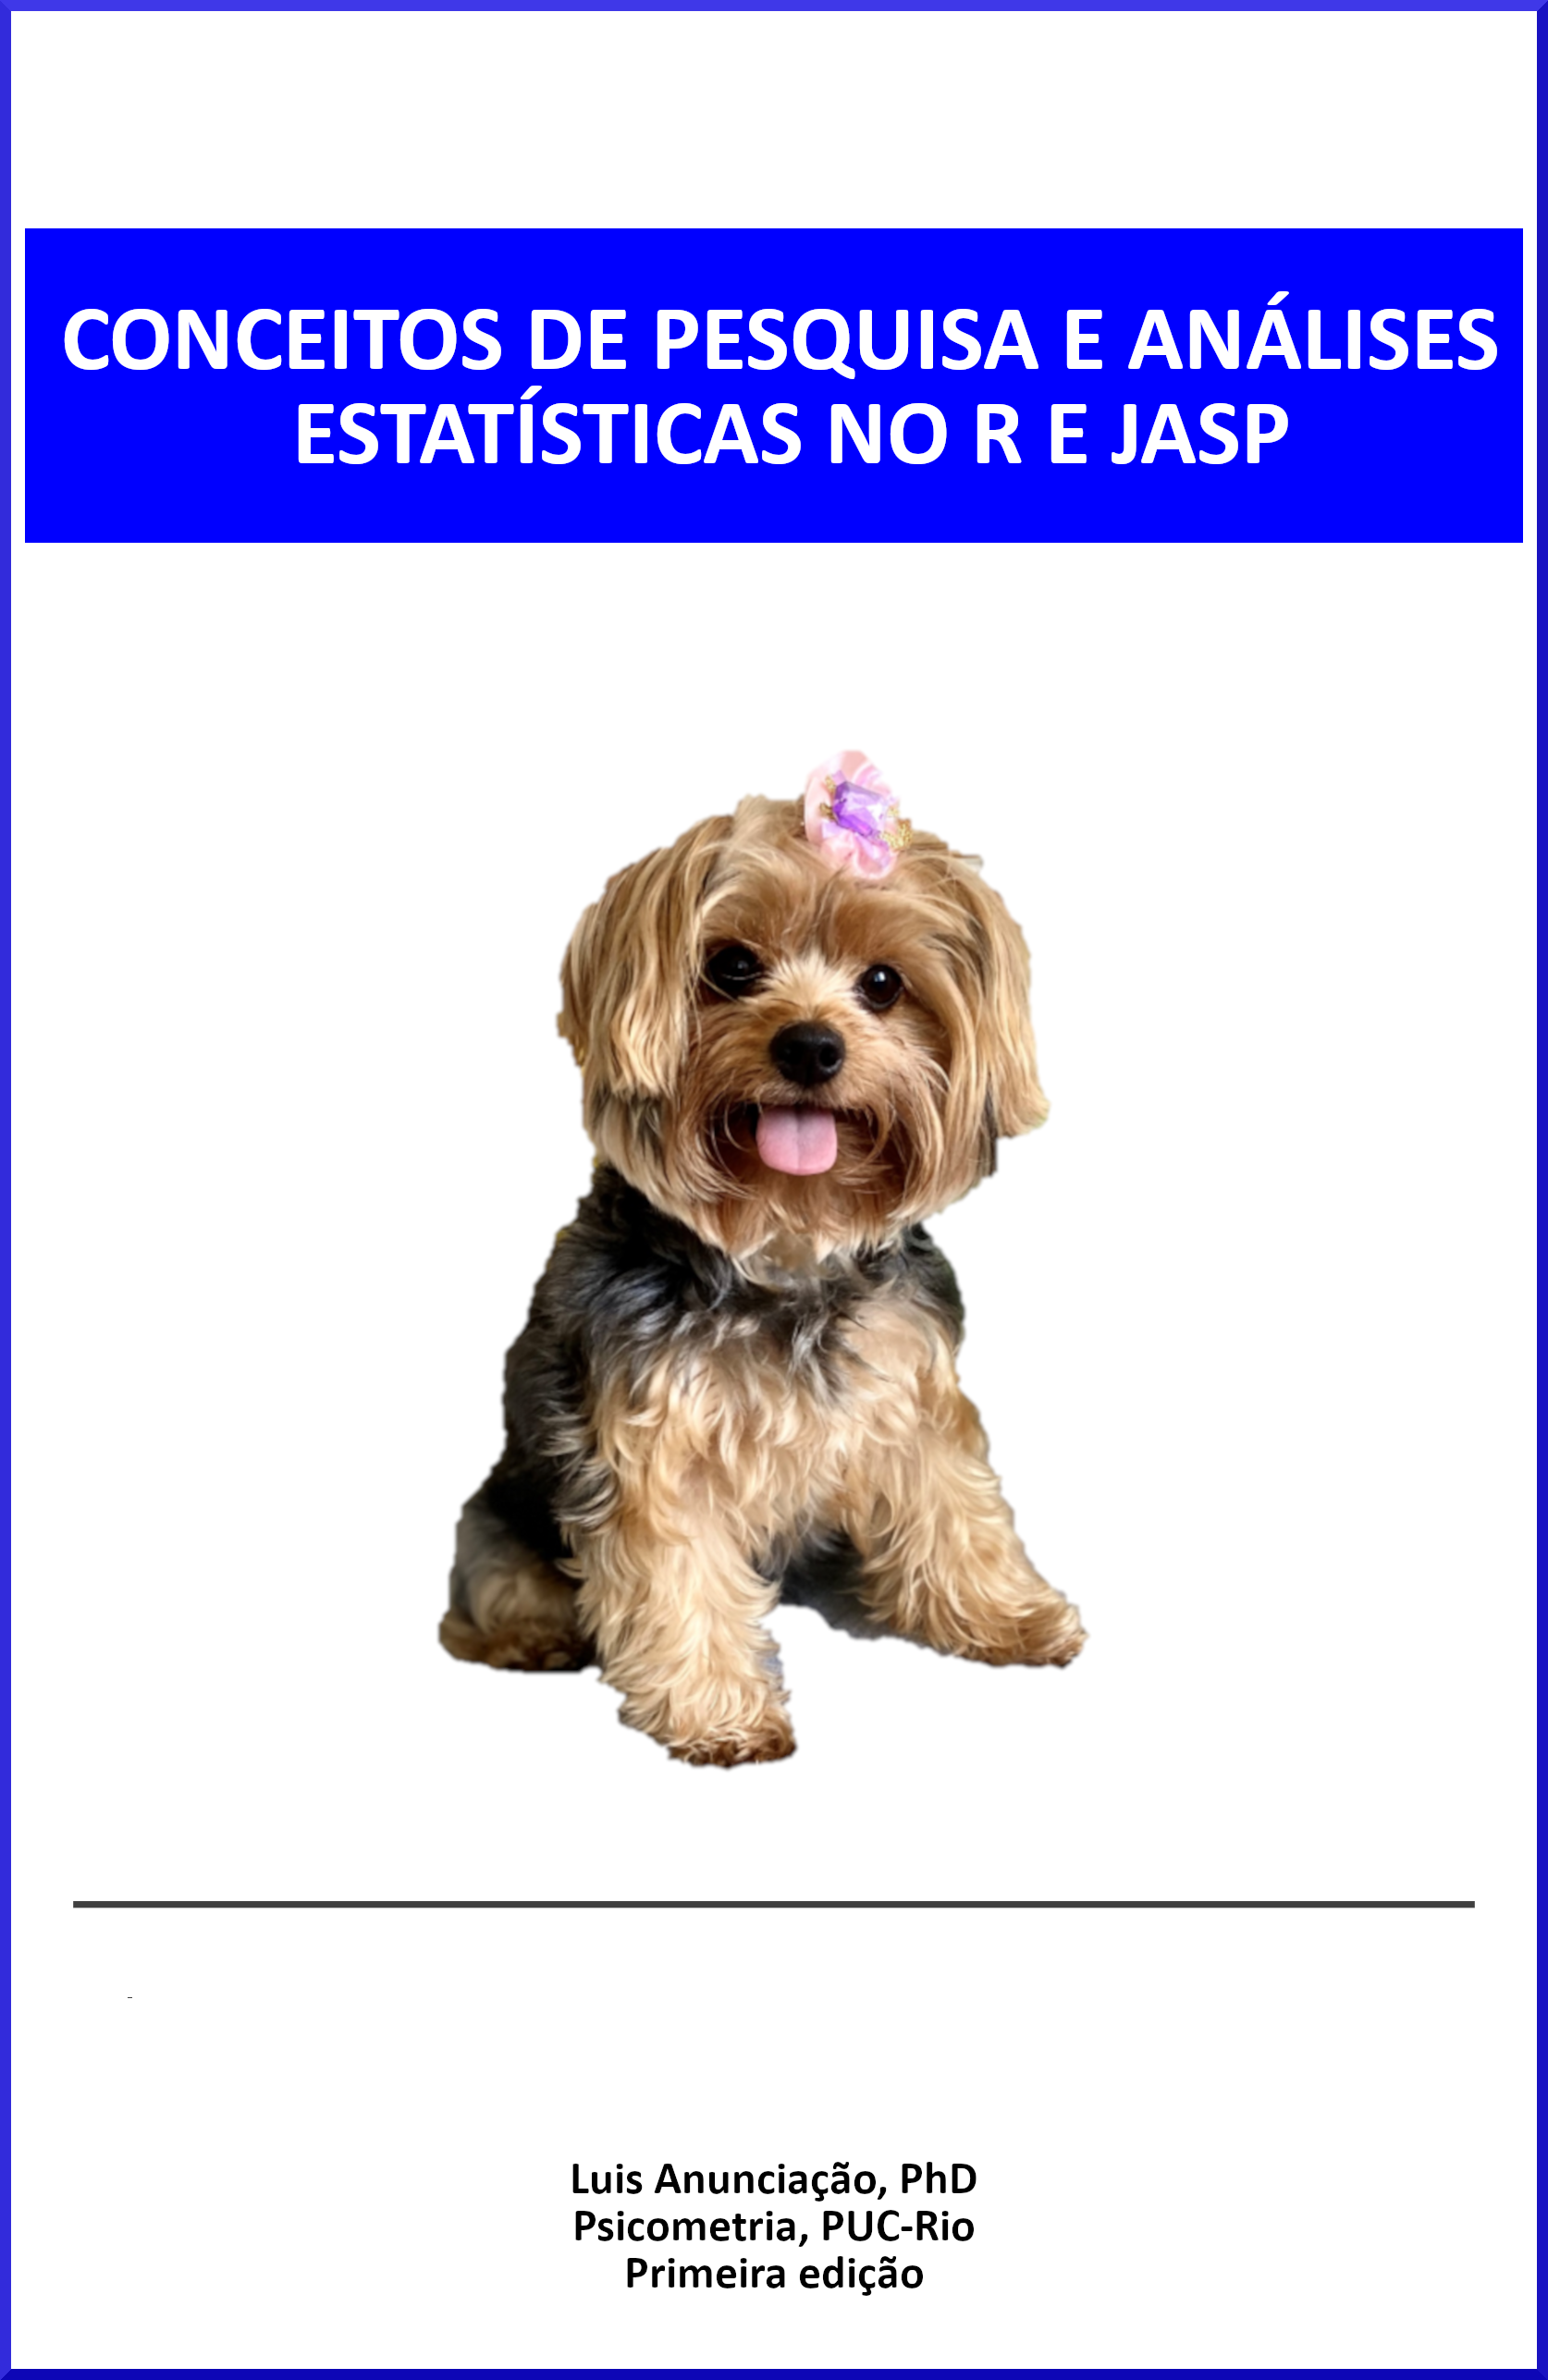
\includegraphics{./img/capa_jolie.png}

\hypertarget{atenuxe7uxe3o}{%
\section{Atenção}\label{atenuxe7uxe3o}}

Atenção: Leia com cuidado. Este livro ainda está em sua fase de revisão.\\
Última modificação: 05 March, 2021 às 19:35

\hypertarget{a-proposta}{%
\section{A proposta}\label{a-proposta}}

Este livro nasceu como um dos principais e mais frutíferos resultados das aulas de graduação e pós-graduação ministradas por mim em alguns locais, mas com maior intensidade na PUC-Rio, UFRJ e IBNeuro. Por bastante tempo, nas aulas de estatística aplicada à Psicologia e Bioestatística, eu recorri a diferentes livros que, cada qual a sua maneira, apresentavam conceitos de pesquisa, técnicas estatísticas e análise de dados.

No entanto, acabei percebendo (ou tendo a impressão) de que eles apresentam a estatística por diferentes atalhos pedagógicos, (1) sugerindo que pesquisa e estatística eram áreas distantes, (2) que toda estatística podia ser resumida por testes de hipóteses independentes entre si e que (3) situações envolvendo dados reais não tinham tanto interesse. No geral, parece-me que para eles apresentarem a estatística na ciência, era necessário se distorcer pesadamente a ciência da estatística.

Em função disso, nos últimos anos, eu fui sentindo necessidade de apresentar os conceitos de pesquisa e técnicas estatísticas de forma integrada, contanto com dados reais e seguindo por uma metodologia de aula que pudesse ser pragmática, mas sem reforçar vícios inadequados sobre conceitos de estatística.

Conciliar essas condições em um único livro de maneira adequada é bastante improvável. Dessa forma, esse livro opta por uma abordagem majoritariamente pragmática, mas que evita se distanciar de conceitos teóricos. O pragmatismo é fundamental para que o estudante consiga, rapidamente, entender os procedimentos relacionados à análise de dados e implementar técnicas estatísticas para tomar decisões. Quão antes o estudante entender a utilidade da estatística para resolver problemas, maior é a probabilidade dele vir a gostar da área. Por sua vez, os aspectos teóricos são os alicerces para que o estudante possa perceber também que a utilidade que a estatística tem na ciência só é possível por ela ser uma disciplina sólida e robusta e que veio se aprimorando nas últimas décadas.

Isso posto, este livro é fruto de um grande esforço que tem a proposta de ser um manual técnico, em que são apresentados conceitos de pesquisa e análises estatísticas realizadas no R e no JASP e com especial aplicação em Psicologia e Bioestatística. Em cada capítulo, o estudante terá a oportunidade de acessar:

\begin{enumerate}
\def\labelenumi{\arabic{enumi}.}
\tightlist
\item
  Uma pesquisa científica, explicitando o problema e as hipóteses que a guiaram\\
\item
  O artigo publicado com os resultados\\
\item
  A base de dados em formato R ou CSV para reprodução das análises\\
\item
  O conjunto de procedimentos estatísticos utilizados\\
\item
  Recursos extras para aprofundamento em tópicos específicos\\
\item
  Exercícios que auxiliem no entendimento do conteúdo, quase sempre retirados de provas externas
\end{enumerate}

Com isso, o livro oferece ao estudante um ambiente em que ele possa resolver um problema real, utilizando as técnicas e métodos estatísticos como ferramentas para tomada de decisão. Apesar do foco ser mais no problema de pesquisa do que nas ferramentas analíticas, em todos os capítulos, a aplicação da estatística na ciência será reforçada pela apresentação de alguns conceitos da ciência da estatística.

Espero que este livro possa ser útil a estudantes de graduação e pós-graduação, agradável a leitores de estatística como de Psicologia e um recurso importante para outros docentes que, eventualmente, precisem de um material de apoio.

\hypertarget{objetivo}{%
\section{Objetivo}\label{objetivo}}

O livro tem como objetivos (1) apresentar, (2) discutir e (3) operacionalizar conceitos de pesquisa e análises estatística de dados a partir de pesquisas publicadas e dados reais. Espera-se que qualquer o estudante consiga realizar todas as ações descritas no decorrer dos capítulos de maneira guiada e intuitiva. As sintaxes utilizadas no ambiente R e as telas de execução do JASP são integralmente disponíveis.

\hypertarget{puxfablico-alvo}{%
\section{Público-alvo}\label{puxfablico-alvo}}

Este livro foi desenvolvido de maneira mais focada a estudantes de Psicologia e Bioestatística. As pesquisas e exemplos utilizados são mais aderentes a essas duas áreas. No entanto, como parte dos conceitos e análises implementadas no livro são interdisciplinares, espera-se que estudantes de áreas como educação, administração e economia também possam também ter proveito do livro.

\hypertarget{formato-do-livro}{%
\section{Formato do livro}\label{formato-do-livro}}

O livro foi pensado para ter uma estrutura (1) organizada, (2) linear e (3) formada por capítulos autossuficientes escritos para responder questões específicas. Acredito que, assim, ele possa atender tanto estudantes interessados em ler a obra inteira, como aqueles que buscam informações mais específicas sobre um tópico particular.

Esse formato adotado tende a gerar uma percepção diferente entre aqueles que consultarem apenas um capítulo ou outro e aqueles que lerem o conteúdo por completo. Há uma maior chance disso ocorrer em capítulos sobre testes estatísticos. Uma vez que diversos testes estatísticos são casos particulares de outros, alguns assuntos que parecem destoantes em uma leitura inicial, tornam-se articulados em outros capítulos.

Muitos capítulos recebem o nome de testes de hipóteses (ex: Teste T ou Regressão). Isso foi intencional e visa auxiliar estudantes que precisem apenas de informações pontuais, bem como tende a enfraquecer a ideia de uma relação ponto a ponto tipicamente feita entre testes estatísticos e delineamentos específicos.

\hypertarget{como-usar-este-livro}{%
\section{Como usar este livro}\label{como-usar-este-livro}}

O livro é formado por dois componentes: capítulos teóricos e capítulos voltados à análise de dados. Os capítulos teóricos reúnem alguns conceitos fundamentais de pesquisa e estatística, tais como tipos de variáveis, delineamento de pesquisa e técnicas de amostragem. Estes capítulos foram escritos pensando em alunos de graduação do curso de Psicologia. Tenho a impressão que esses capítulos serão pouco acessados, apesar de importantes.

Os capítulos analíticos são focados em testes de hipóteses e contam com uma metodologia direta ao ponto, em que atividades similares às realizadas nos artigos são demonstradas. Estes capítulos foram desenvolvidos para estudantes de pós-graduação. Acredito que esses capítulos serão bastante acessados.

A figura abaixo diagrama os dois componentes de forma aproximada.

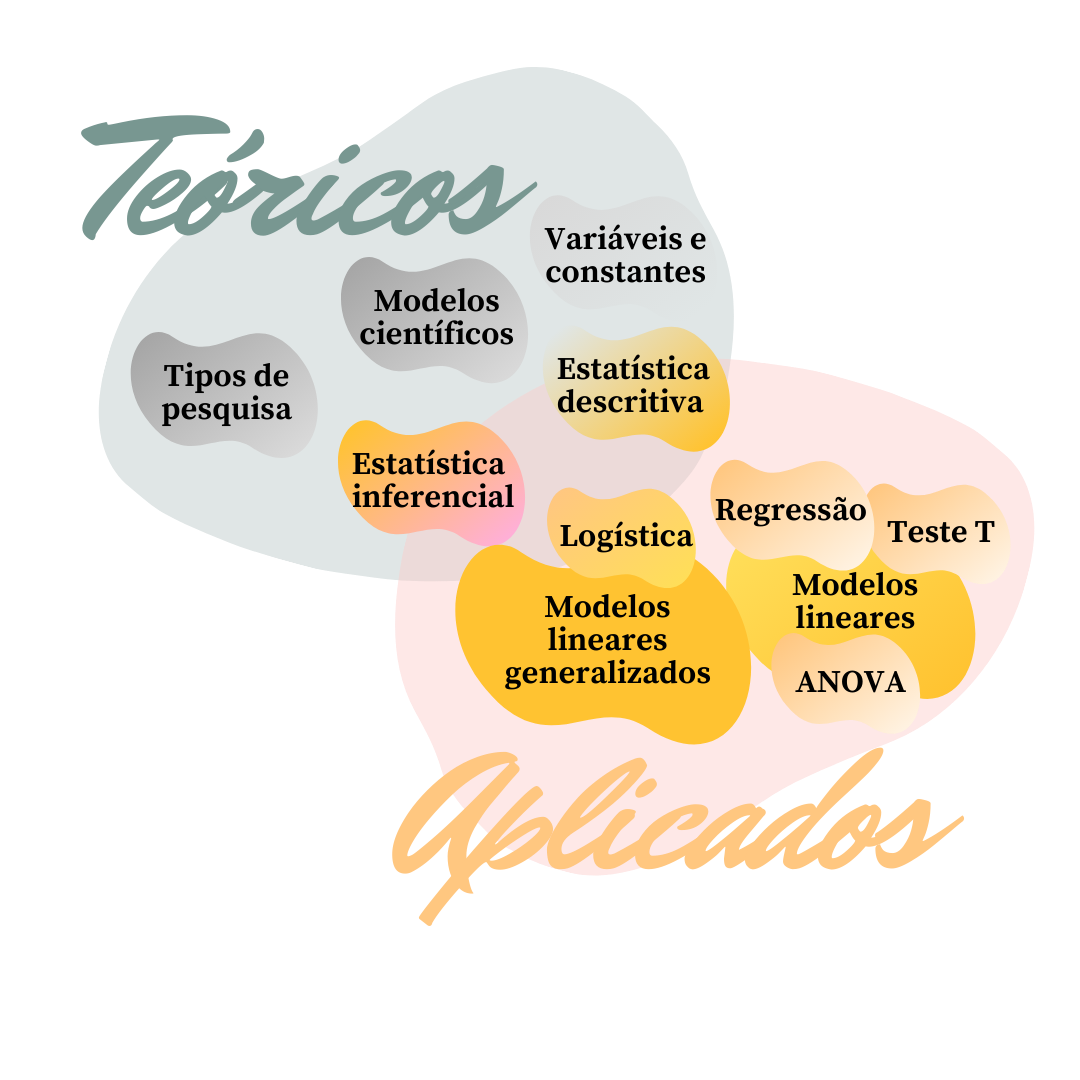
\includegraphics{./img/proposta.png}

\hypertarget{pesquisas-e-dados}{%
\section{Pesquisas e dados}\label{pesquisas-e-dados}}

Neste livro, as seguintes pesquisas e seus materiais são utilizados:

\begin{itemize}
\item
  \href{https://doi.org/10.1590/0102.3772e36412}{``Depression and Anxiety Symptoms in a Representative Sample of Undergraduate Students in Spain, Portugal, and Brazil''}
\item
  \href{https://onlinelibrary.wiley.com/doi/abs/10.1111/cch.12649}{``Confirmatory analysis and normative tables for the Brazilian Ages and Stages Questionnaires: Social--Emotional''}
\item
  \href{https://www.neuropsicolatina.org/index.php/Neuropsicologia_Latinoamericana/article/view/545}{Psychometric properties of a short-term visual memory test (MEMORE)"}
\item
  \href{https://www.metodista.br/revistas/revistas-metodista/index.php/REGS/article/view/6453}{``A relação entre o nível de Empreendedorismo (TEG) e os aspectos sociodemográficos dos Taxistas cooperados da cidade de Santo André/São Paulo, Brasil''}
\item
  \href{https://www.scielo.br/scielo.php?script=sci_arttext\&pid=S0102-09352019000100109}{``Avaliação psicométrica em português do indicador de dor crônica de Helsinki em cães com sinais crônicos de osteoartrite''}
\item
  \href{https://www.researchgate.net/publication/323729370_Aspects_Related_to_Body_Image_and_Eating_Behaviors_in_Healthy_Brazilian_Undergraduate_Students}{``Aspects Related to Body Image and Eating Behaviors in Healthy Brazilian Undergraduate Students''}
\item
  ``Parent-reported diagnosis of Attention Deficit Hyperactivity Disorder and psychostimulant use among children and adolescents: a population-based nationwide study''
\item
  ``Resilience and vulnerability in adolescents with primary headaches: a cross-sectional population-based study''
\end{itemize}

As bases são \emph{Open Science}. Isso significa que elas são gratuitas e universalmente acessíveis para finalidades acadêmicas. Em cada capítulo, as bases irão aparecer na seção ``Pesquisa'', da seguinte maneira:

A base desta pesquisa está disponível em formato \textbf{R (Rdata)} e em \textbf{CSV}, que é lido pelo JASP. Clique na opção desejada.

Base R: \href{}{Base R}\\
Base JASP: \href{}{Base CSV}

As bases em R tem formato .RData e as bases para o JASP tem formato .CSV.

\hypertarget{o-r-e-os-pacotes}{%
\section{O R e os pacotes}\label{o-r-e-os-pacotes}}

O livro é integralmente desenvolvido pelo recurso de ``programação letrada'' no R Markdown, ou seja, ele entrelaça aspectos textuais e linhas de código. Em todos os capítulos, as funções nativas do R e do Tidyverse serão utilizadas. Caso alguém queira reproduzir as análises, será necessário apenas executar as linhas de código disponíveis no decorrer do livro.

O \texttt{tidyverse} costuma ter atualizações frequentes. Caso um alerta de \texttt{deprecated} seja apresentado, isso significa que a função utilizada foi parcialmente desativada, o que não costuma impactar nas análises.

\hypertarget{jasp}{%
\section{JASP}\label{jasp}}

O JASP é um programa gratuito que tem sido cada vez mais utilizado em Psicologia. Ele é feito integralmente por código aberto e sua interface é bastante amigável e intuitiva. Ao instalar o JASP, o R também será instalado em seu computador e ficará no pano de fundo. Dessa maneira, todas as ações feitas por \emph{Point and Click} no JASP, serão convertidas em linhas de código no R e apresentadas de maneira dinâmica no JASP.

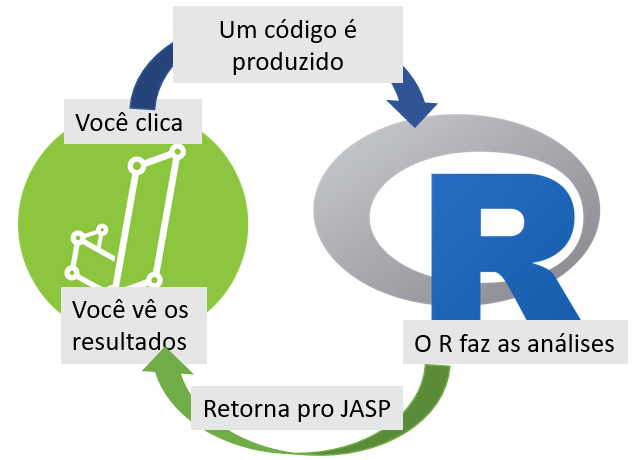
\includegraphics{./img/capa_r_jasp.png}

Em todos os capítulos, telas do JASP serão apresentadas para que seja possível a reprodução integral de algumas análises. Da mesma forma que qualquer pacote estatístico, o JASP é atualizado frequentemente. Esse livro contou com a versão 0.14.1 e espero que futuras atualizações não comprometam a proposta do livro.

\hypertarget{outros-recursos}{%
\section{Outros recursos}\label{outros-recursos}}

Em cada um dos capítulos, aplicações da estatística e referências bibliográficas serão apresentadas. Tenha em mente que há um debate intenso em diferentes conceitos de estatística, da mesma forma que muitas condições computacionais podem aparecer durante a execução das análises propostas. Eu recomendo fortemente a comunidade \href{https://stackoverflow.com/}{stackoverflow} como um recurso pedagógico para auxiliar em ambos os cenários.

Questões relacionadas aos capítulos são listadas de forma a conectar o conteúdo do livro com exigências balizadas por critérios externos, tal como o ENADE e bancas de concurso.

\hypertarget{capa}{%
\section{Capa}\label{capa}}

Por tradição, livros de Ciência de Dados e Estatística utilizam a imagem de algum animal na capa. Há livros com cachorros, papagaios, peixes, carangueijos, lagartos, etc. Esse livro não foge dessa regra e tem como capa a Jolie, a minha cachorrinha com a Anna. Ela foi indispensável para o atraso ao término deste livro.

\hypertarget{versuxe3o-do-livro}{%
\section{Versão do livro}\label{versuxe3o-do-livro}}

Como todos os livros, este também tem uma história de desenvolvimento. A tabela abaixo apresenta a versão, a data de lançamento e algumas características importantes.

\begin{longtable}[]{@{}lll@{}}
\toprule
\begin{minipage}[b]{0.24\columnwidth}\raggedright
Versão\strut
\end{minipage} & \begin{minipage}[b]{0.34\columnwidth}\raggedright
Data\strut
\end{minipage} & \begin{minipage}[b]{0.34\columnwidth}\raggedright
Características\strut
\end{minipage}\tabularnewline
\midrule
\endhead
\begin{minipage}[t]{0.24\columnwidth}\raggedright
Beta 1\strut
\end{minipage} & \begin{minipage}[t]{0.34\columnwidth}\raggedright
Fevereiro, 2020\strut
\end{minipage} & \begin{minipage}[t]{0.34\columnwidth}\raggedright
Primeira versão. Baixa revisão textual e dos conceitos estatísticos. Erros são esperados. A utilização deve ser feita apenas de maneira incipiente\strut
\end{minipage}\tabularnewline
\bottomrule
\end{longtable}

\hypertarget{autor}{%
\section{Autor}\label{autor}}

\href{http://lattes.cnpq.br/3982200733248687}{Luis Anunciação} é doutor em Psicometria pela Pontifícia Universidade Católica do Rio de Janeiro (PUC-Rio), com intercâmbio na University of Oregon, mestre em saúde pública pela Universidade do Estado do Rio de Janeiro e especialista em Neuropsicologia (IBNeuro) e Bioestatística (Johns Hopkins University). Atualmente, é professor do Departamento de Psicologia da PUC-Rio, coordenador da ANOVA e psicometrista da Nila Press, uma editora especialzada no desenvolvimento de instrumentos psicológicos.

\hypertarget{revisuxe3o-tuxe9cnica}{%
\section{Revisão técnica}\label{revisuxe3o-tuxe9cnica}}

Este livro contou com a revisão técnica do Dr.~J. Landeira-Fernandez (Doutor em Neurociências pela University of California - UCLA, Pesquisador 1A do CNPq) e Ms.~Regina Albanense (Graduada em Matemática e Estatística e Mestre em Ciências). Dr.~Landeira foi fundamental em tópicos envolvendo aspectos de pesquisa e análises estatísticas e Ms.~Regina foi fundamental para revisão da modelagem matemática e revisão conceitual.

\hypertarget{agradecimentos}{%
\section{Agradecimentos}\label{agradecimentos}}

Nenhum homem é uma ilha. Este livro só foi possível graças a um conjunto de pessoas que auxiliaram e fizeram uma profunda revisão do texto. Meus sinceros agradecimentos a (ao):

J. Landeira-Fernandez, PUC-Rio\\
Regina Albanense, CONRE\\
Cristiano Fernandes, PUC-Rio\\
Danilo Assis Pereira, IBNeuro\\
Anna Carolina de Almeida Portugal, UFRJ\\
Emanuel Cordeiro, UFPE\\
Alunos da PUC-Rio, UFRJ, IBNeuro e ANOVA

\hypertarget{programas-estatuxedsticos}{%
\chapter{Programas estatísticos}\label{programas-estatuxedsticos}}

\textbf{Objetivos do capítulo}\\
1. Apresentar os programas estatísticos utilizados durante o livro\\
2. Discutir características do R, tidyverse e seus pacotes\\
3. Discutir características do JASP

Programas estatísticos são ferramentas indispensáveis tanto na gestão, como na análise dos dados resultantes de uma pesquisa. Eles servem para otimizar o tempo gasto nas etapas analíticas de uma pesquisa, apesar de, em menor escala, permitirem a execução de análises inadequadas. No dia a dia de um pesquisador, apenas muito raramente as análises são feitas manualmente. Dessa maneira, o conhecimento de programas de análise de dados faz parte das competências esperadas para quem deseja ou precisa trabalhar com estatística.

Atualmente, há muitos programas e pacotes estatísticos disponíveis para uso. Acredito que a maioria deles tenha mais similaridades do que diferenças e produzam resultados confiáveis. Neste livro, o R e o JASP serão utilizados e algumas de suas características serão descritas neste capítulo.

\hypertarget{o-r}{%
\section{O R}\label{o-r}}

O R é uma linguagem de programação focada em análises estatísticas, que vem ganhando popularidade entre pesquisadores e cientistas. Este livro foi integralmente feito e baseado no ambiente R que, apesar de ainda não ser o programa mais frequente em Psicologia, apresenta diversas vantagens em comparação aos programas mais usuais.

\begin{itemize}
\item
  o R e todos os seus pacotes e otimizações são gratuitos.
\item
  o R é uma linguagem de programação desenvolvida especificamente para Estatística.

  \begin{itemize}
  \tightlist
  \item
    Diferente de uma linguagem mais geral (por exemplo, Python) ou de um programa \emph{point and click}, o R é uma linguagem focada em análise estatística. Ao se programar utilizando o R, o usuário tem controle total das ações realizadas e dos resultados obtidos. Assim, raramente o R apresentará resultados excessivos e distantes das análises solicitadas. Apesar disso poder assustar no início, acredito que essa característica seja essencial e, inclusive, serve como um excelente auxílio pedagógico para que o estudante planeje adequadamente as análises de interesse, em vez de apenas selecionar parte de um \emph{output} padronizado, como ocorre com o SPSS.
  \end{itemize}
\item
  O R é um programa de nicho em Estatística. Essa característica faz com que ele seja absolutamente adaptado para o dia a dia em estatística, incluindo não apenas análises descritivas e inferenciais, mas também análises para simulação e controle de resultados.
\item
  O R permite o desenvolvimento de interfaces web e aplicativos.
\item
  O R tem diversos pacotes.

  \begin{itemize}
  \tightlist
  \item
    Pacotes são complementos que permitem otimizar as análises que o R faz. A comunidade R tem um exército de pacotes, que além de gratuitos, foram verificados publicamente. O ambiente CRAN (\emph{The Comprehensive R Archive Network}) é o local em que estes pacotes estão alocados. Neste livro, todos os capítulos contam com pacotes específicos, que permitiram que análises complexas fossem realizadas com poucos comandos.
  \end{itemize}
\item
  O R possui uma enorme comunidade de apoio.

  \begin{itemize}
  \tightlist
  \item
    Os usuários do R formam uma rede muito dinâmica e que oferece grande apoio em caso das mais diversas dúvidas. A comunidade \href{https://stackoverflow.com/}{stackoverflow} talvez seja a mais voluma e reúne pessoas de todas as nacionalidades.
  \end{itemize}
\end{itemize}

Para baixar o R, é necessário ir no site \url{https://cran.r-project.org/}. Em seguida, para baixar o R Studio, é necessário acessar \url{https://rstudio.com/}.

\hypertarget{tidyverse}{%
\section{Tidyverse}\label{tidyverse}}

O Tidyverse é um ambiente de pacotes. Eles funcionam de maneira totalmente integrada e permitem que a estrutura da programação seja mais intuitiva e próxima à forma pela qual pensamos. No Tidyverse, os códigos seguem a lógica de sujeito + verbo e permitem uma programação encadeada, ao se utilizar a ligação \emph{pipe} (\texttt{\%\textgreater{}\%}). Ao instalar o tidyverse \texttt{install.package("tidyvese")}, os pacotes abaixo ficam disponíveis no R.

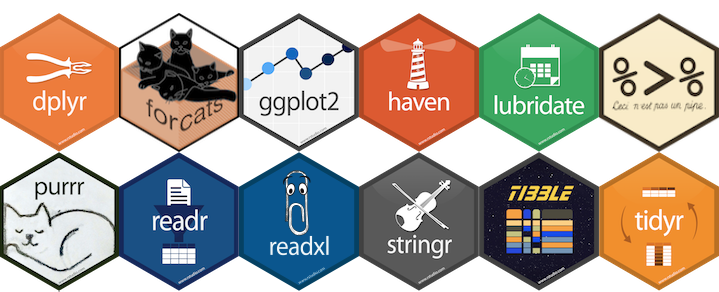
\includegraphics{./img/tidyverse_website.PNG}

\hypertarget{dificuldades-esperadas}{%
\section{Dificuldades esperadas}\label{dificuldades-esperadas}}

Algumas dificuldades são esperadas quando se trabalha programação no geral e com o R especificamente. Apesar do R e seus pacotes oferecem excelentes ferramentas para análise de dados, algumas condições descritivas são demasiadamente custosas. Por exemplo, enquanto realizar algumas tabelas e gráficos no Excel é tremendamente fácil, com alguma frequência o R exige diversas linhas de código para isso.

Nesse sentido, na relação entre dificuldade e complexidade, o R sai na frente em tarefas complexas (como exemplo, estimar os coeficientes de um modelo não-linear), mas talvez perca em tarefas fáceis (por exemplo, gerar uma tabela de contingência). A Figura a seguir apresenta esta relação comparando as análises feitas no R e no Excel.

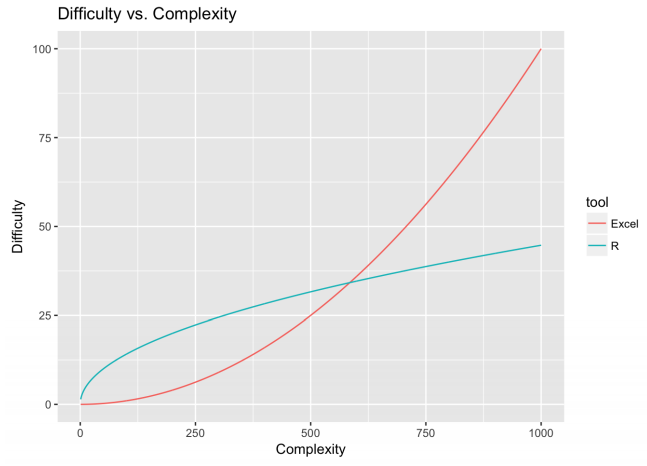
\includegraphics{./img/excel_r.PNG}

Além disso, o R traz uma outra barreira importante em aspectos que envolvam o ensino de estatística, especialmente na graduação. Como o R é uma linguagem de programação, o estudante teria de aprender a programar antes de conseguir entender conceitos de pesquisa e a utilidade da estatística. Isso poderia impactar negativamente na motivação do estudante, principalmente àqueles com uma aversão \emph{a priori} da matéria,

Em situações como esta, talvez o ideal seja começar motivando o estudante a entender como a estatística é uma ferramenta importante para tomar decisões para, só depois e lentamente, apresentar aspectos matemáticos e computacionais.

\hypertarget{verbos-do-dplyr}{%
\section{Verbos do dplyr}\label{verbos-do-dplyr}}

Entre os pacotes do ambiente tidyverse, o dplyr é o que será mais utilizado. Este pacote funciona de maneira muito intuitiva, em que as funções dependem de uma estrutura \texttt{sujeito\ \%\textgreater{}\%\ verbo(complemento)}. Essa é uma diferença importante em relação ao R Base. Por exemplo, no R Base é necessário executar \texttt{names(dataset)} para verificar as variáveis de um conjunto de dados. Pelo dplyr deve-se utilizar \texttt{dataset\ \%\textgreater{}\%\ names}.

O dplyr funciona a partir de verbos declarativos e os principais estão listados na tabela a seguir. As sintaxes deixadas no decorrer do livro também permitem uma melhor apreensão das funcionalidades.

\begin{longtable}[]{@{}ll@{}}
\toprule
Verbo & Ação\tabularnewline
\midrule
\endhead
glimpse & Inspeciona os dados\tabularnewline
count & Conta os níveis de uma variável\tabularnewline
select & seleciona uma variável específica\tabularnewline
filter & Filtra os resultados por um nível específico de uma variável\tabularnewline
group\_by & Agrupa os resultados por níveis de uma variávei específica\tabularnewline
summarise & Apresenta sumários (com medidas estatísticas)\tabularnewline
mutate & Cria novas variáveis ou altera as existentes\tabularnewline
arrange & Organiza a apresentação dos resultados\tabularnewline
left\_join & Junta bases ou colunas\tabularnewline
pivot\_longer & Transforma uma base larga em longa\tabularnewline
pivot\_wider & Transforma uma base longa em larga\tabularnewline
\bottomrule
\end{longtable}

\emph{Nota: Em alguns momentos, em função da praticidade computacional, algumas sintaxes vão contar com o formato base do R.}

É importante ficar atento às atualizações do dplyr e do sistema tidyverse como um todo. Eventualmente, mudanças podem ocorrer e impossibilitar (ou dificultar) a reprodução de rotinas antigas.

\hypertarget{o-jasp}{%
\section{O JASP}\label{o-jasp}}

O JASP é um programa gratuito, com uma interface amigável, \emph{point and click} e altamente versátil para a maioria das análises realizadas. A versão utilizada neste livro é a 0.14.1. O JASP foi desenvolvido por um time de psicólogos e estatísticos liderados pelo Prof.~Eric-Jan Wagenmakers, da Universidade de Amsterdam. Isso talvez explique o motivo pelo qual o JASP vem sendo cada vez mais utilizado em análises de dados psicológicos e na docência de matérias relacionadas a métodos estatísticos.

Para baixar o JASP, é necessário acessar \url{https://jasp-stats.org/download/}.

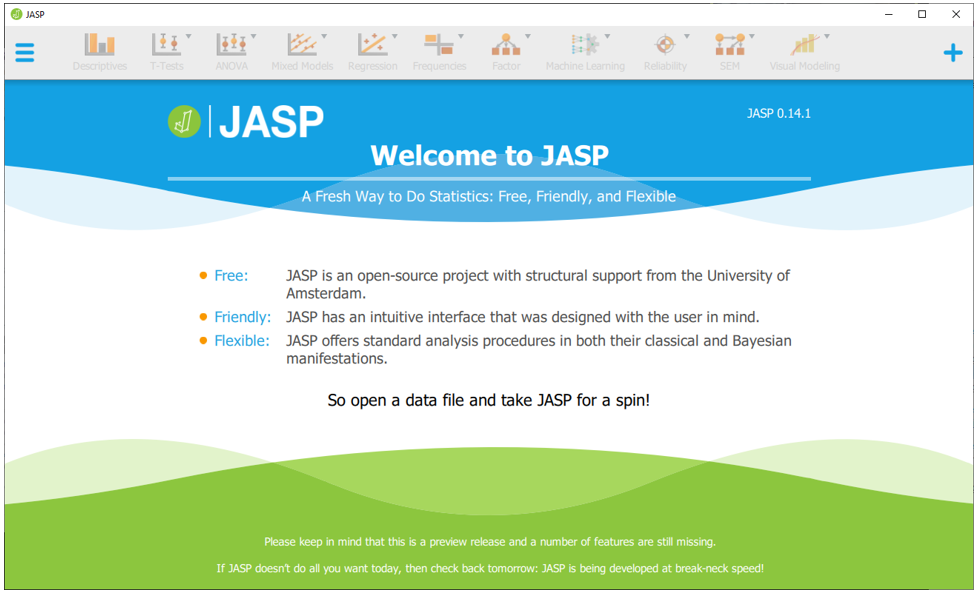
\includegraphics{./img/cap_jasp_interface.png}

Quando se instala o JASP no computador, se instala também o R. Todas as ações feitas no JASP se transformam em linhas de código que são enviadas ao R e, em seguida, retornam pro JASP e são apresentadas na tela. Isso ocorre de maneira instantânea e não há nenhum incômodo para o usuário. Na maioria das vezes, computadores pessoais conseguem rodar o JASP sem grandes problemas.

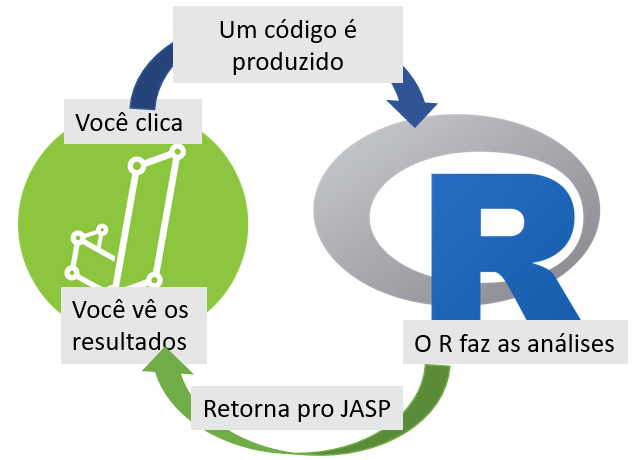
\includegraphics{./img/capa_r_jasp.png}

O idioma oficial do JASP é o inglês e, nesta versão, não pode ser alterado. Para fazer qualquer análise, é necessário carregar um arquivo de dados. Isso pode ser feito no símbolo das três linhas, localizado na parte superior à esquerda.

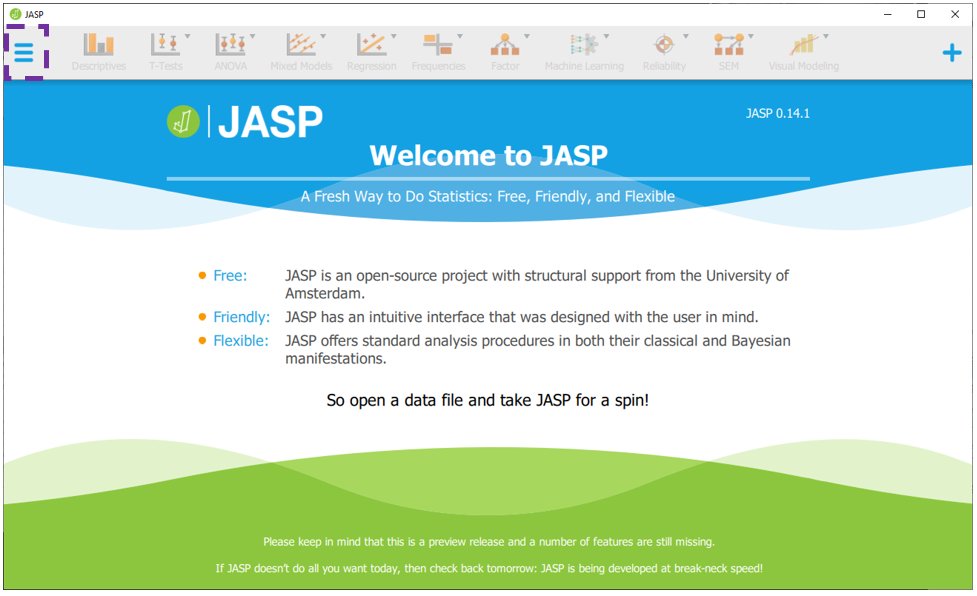
\includegraphics{./img/cap_jasp_abrir.png}

A opção \texttt{open} permite que se acesse algum diretório local específico ou se baixe os dados diretos da plataforma \emph{Open Science Framework (OSF)}. Esta versão do JASP aceita, majoritariamente, arquivos em CSV, que indica que os dados são separados por vírgulas.

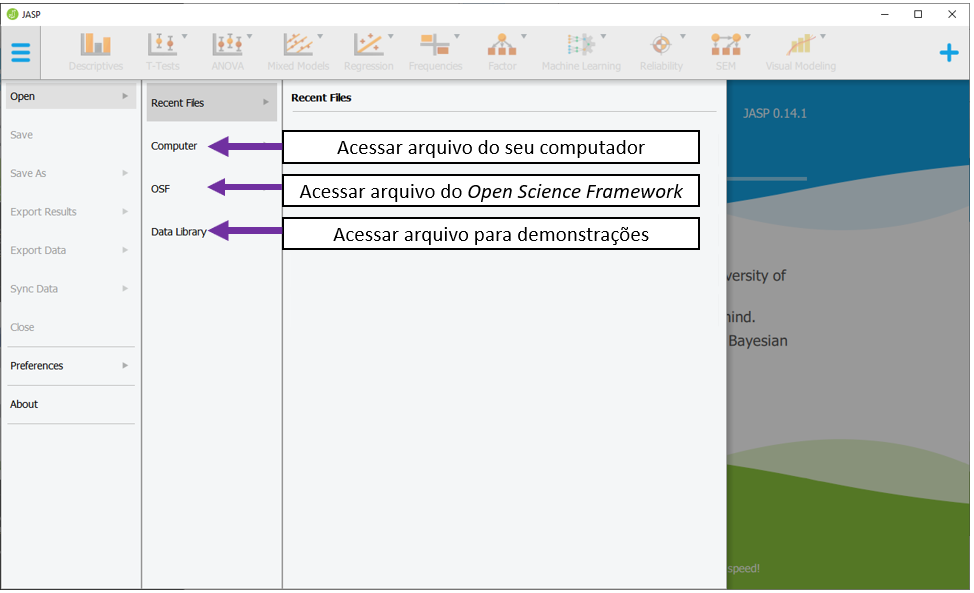
\includegraphics{./img/cap_jasp_abrir2.png}

Ao abrir algum arquivo de dados, o JASP irá apresentar os dados no centro do programa e as opções de análise na parte superior. Tenha atenção que essas telas podem variar de versão para versão.

Em relação aos dados, quase sempre o formato utilizado é o largo. Neste formato, cada coluna representa uma variável, cada linha representa um caso e cada célula (ou vetor) apresenta um valor específico.

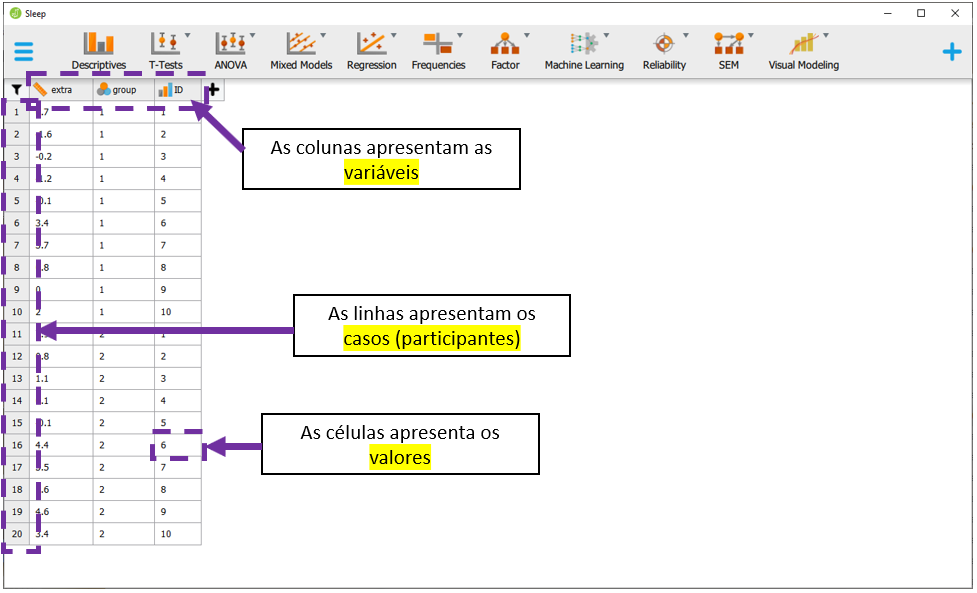
\includegraphics{./img/cap_jasp_dados.png}
O JASP adota uma simbologia específica para definir a escala (ou nível) de medida das variáveis. Isso pode ser visto no símbolo ao lado dos nomes das variáveis. Para alterar o nível, basta clicar sobre o símbolo.

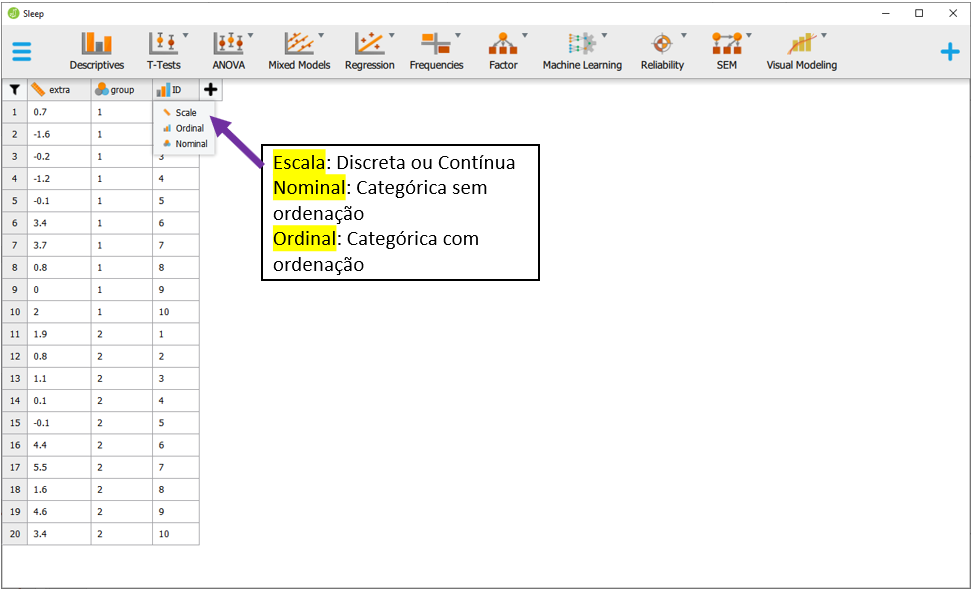
\includegraphics{./img/cap_jasp_tipo_de_dados.png}

É possível também alterar valores e rótulos das variáveis. Para isso, basta clicar no centro da variável. Uma seção na parte de cima do programa será exibida. Para fechar, é necessário clicar no X ao lado direito.

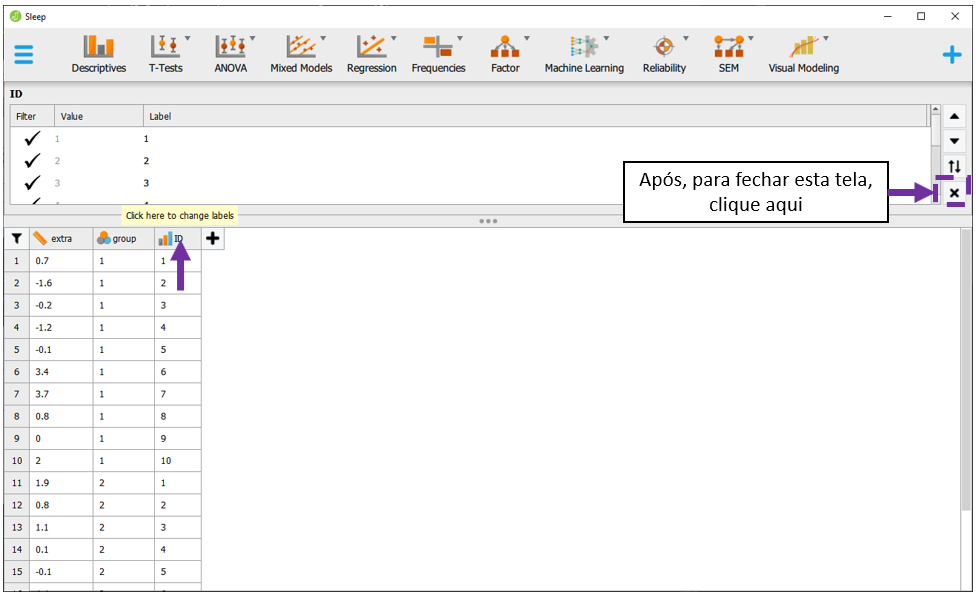
\includegraphics{./img/cap_jasp_alterar_valores.png}

Na parte superior, o JASP oferece as análises possíveis. As opções podem variar de versão para versão, mas as principais tendem a ser as seguintes.

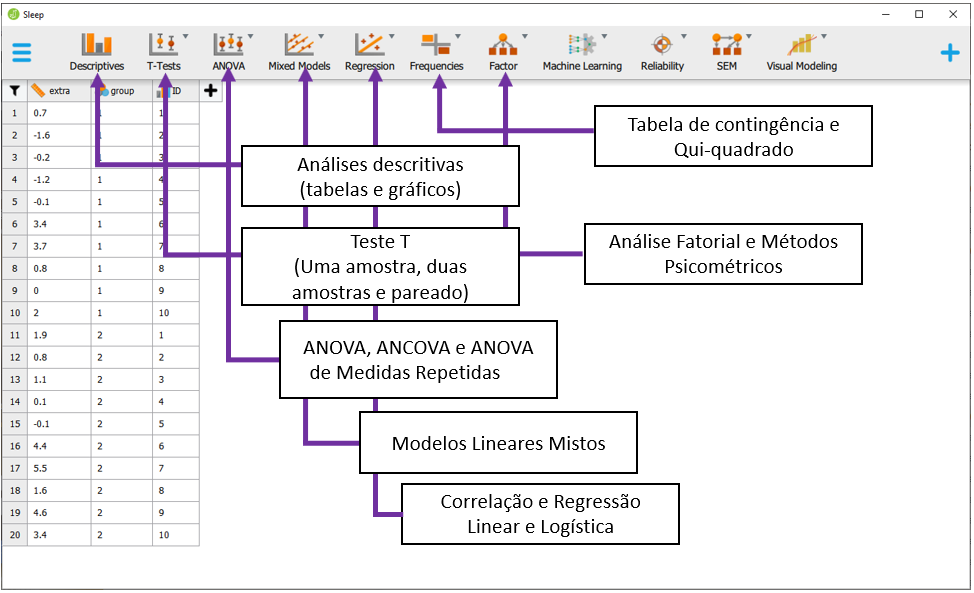
\includegraphics{./img/cap_jasp_features.png}

É possível adicionar módulos e complementos no JASP. Essas adições funcionam de maneira análoga aos pacotes do R. Para fazer isso, basta clicar na cruz azul ao lado direito.

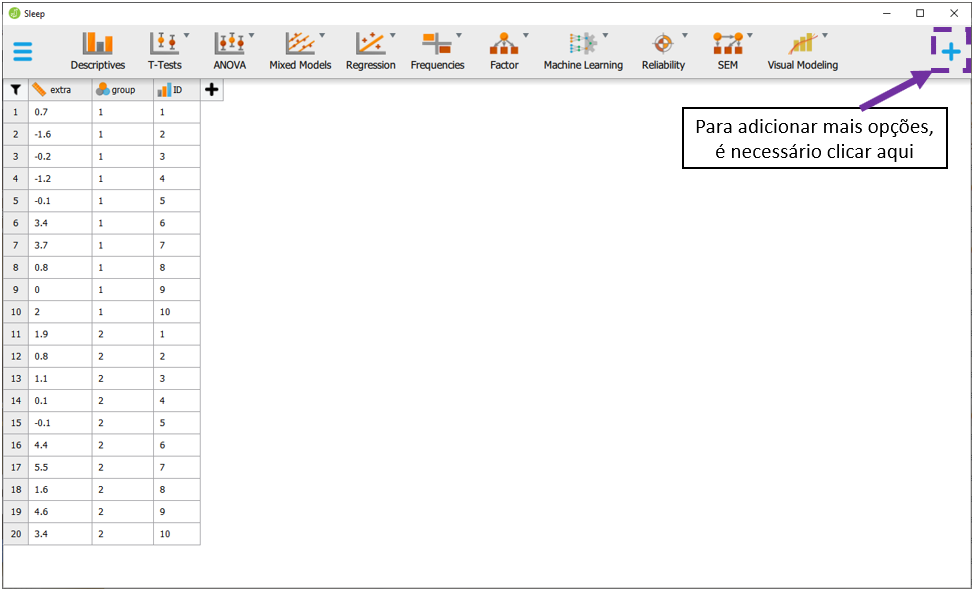
\includegraphics{./img/cap_jasp_adicionar_modulos.png}

Uma barra ao lado direito irá ser exibida. Qualquer opção pode ser selecionada e, ao fazer isso, novos botões irão aparecer na parte superior do programa.

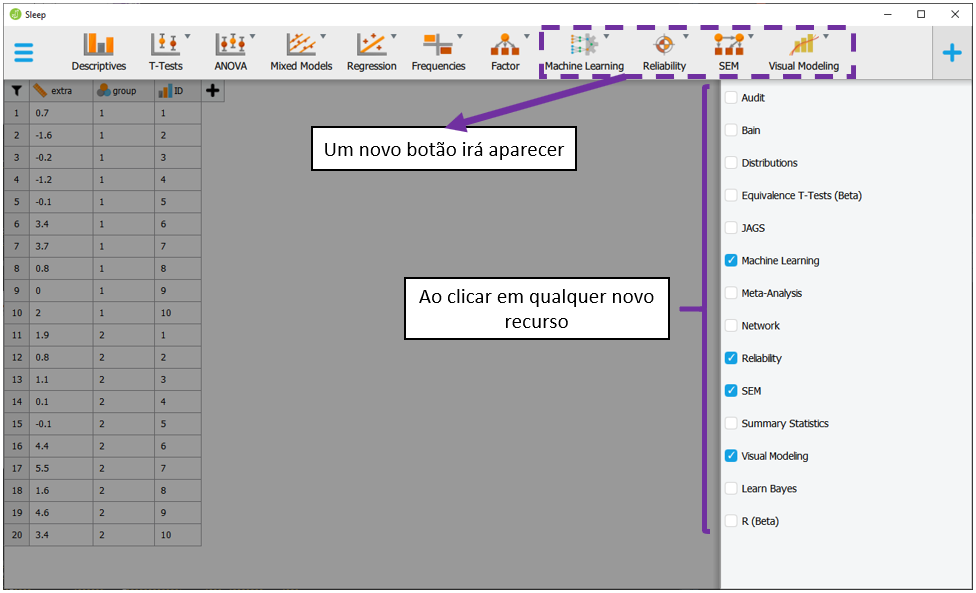
\includegraphics{./img/cap_jasp_adicionar_modulos2.png}

Finalmente, para salvar o trabalho realizado em uma sessão, deve-se clicar na símbolo de três linhas azuis e, em seguida, clicar em \texttt{Save\ as} e selecionar a pasta.. Por padrão, o formato do arquivo sera *.jasp.

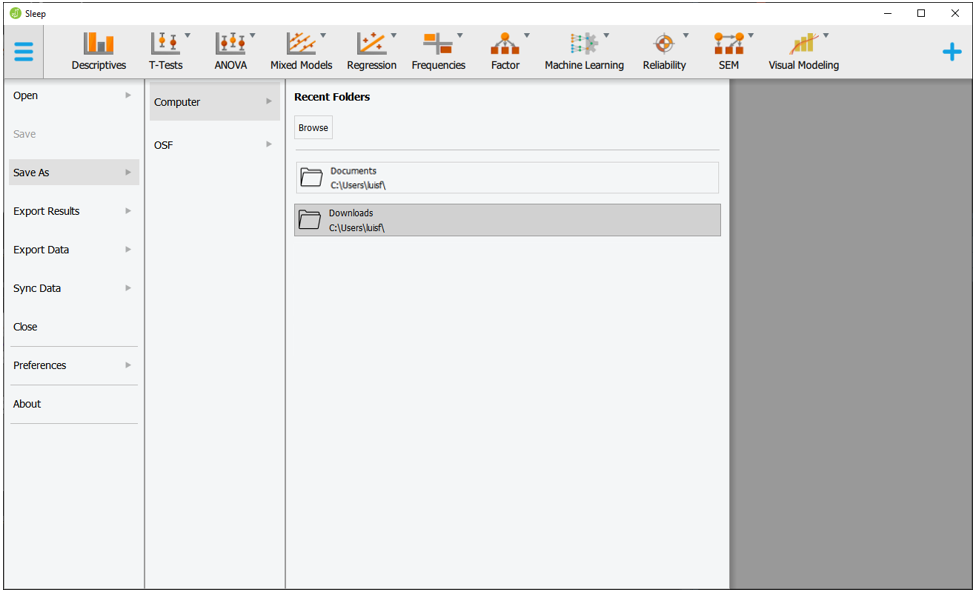
\includegraphics{./img/cap_jasp_salvar.png}

\hypertarget{resumo}{%
\section{Resumo}\label{resumo}}

\begin{enumerate}
\def\labelenumi{\arabic{enumi}.}
\tightlist
\item
  Há muitos programas e pacotes de estatística. Neste livro, o R e o JASP serão utilizados.\\
\item
  O R é gratuito e pode ser complementado por pacotes adicinais.\\
\item
  O tidyverse servirá como principal ecossistema de programação.\\
\item
  O JASP tem recebido grande atenção especialmente em Psicologia e as análises também serão feitas nele.\\
\end{enumerate}

\hypertarget{aspectos-gerais}{%
\chapter{Aspectos gerais}\label{aspectos-gerais}}

\textbf{Objetivos do capítulo}\\
1. Apresentar conceitos transversais encontrados em pesquisa e estatística\\
2. Descrever as variáveis em função de seu relacionamento, escala de medida e capacidade numérica\\
3. Introduzir o debate sobre a escala de medida em Psicologia\\
4. Apresentar as duas principais áreas da estatística

\textbf{GLOSSÁRIO}\\
\textbf{Pesquisa}: Procedimento racional e sistemático de investigação que visa proporcionar respostas específicas a um conjunto de problemas propostos.\\
\textbf{Modelo teórico}: Representação visual, matemática, computacional ou experimental de um sistema de ideias, eventos ou fenômenos.\\
\textbf{Instrumentos científicos}: Ferramentas que permitem amplificar o fenômeno de interesse, além de acessar aspectos da realidade que não podem ser percebidos diretamente.\\
\textbf{Variável aleatória}: É uma variável que está associada a uma distribuição de probabilidade.\\
\textbf{Variável}: Termo genérico usado para se referir às características que estão sendo investigadas ou para se referir às variáveis aleatórias.\\
\textbf{Variável Independente (VI)}: Característica que está sendo manipulada. Entende-se que ela influencia, afeta ou determina outras variáveis.\\
\textbf{Variável dependente (VD)}: Variável que sofre efeito da VI. Seus valores dependem dos níveis da VI.\\
\textbf{Delineamento de pesquisa} Forma de esquematizar o planejamento da pesquisa, especialmente considerando o acesso e controle das variáveis, bem como a coleta e análise de dados.

Quando as pessoas começam seus estudos em estatística, parece haver uma falsa crença de que a estatística é uma área exclusivamente desenvolvida para analisar dados obtidos em uma pesquisa. Este pensamento acaba por produzir uma dicotomia entre pesquisa e estatística, fazendo com que algumas pessoas pensem que as atividades feitas em estatística somente começam após o termino de uma pesquisa. No entanto, isso não é verdade. Apesar da análise de dados ser uma tarefa intensamente feita em estatística, a atuação desta ciência é muito mais ampla do que apenas isso e ocorre em todas as etapas de uma pesquisa.

Em linhas gerais, a estatística é a ciência que fornece os princípios e a metodologia para coleta, organização, apresentação, resumo, tratamento, análise e interpretação de dados. O mnemônico CORRETA quase sempre ajuda a fixar esta definição, já que C se refere à coleta, O se refere à organização, R se refere à resumo, T se refere à tratamento e A se refere à análise, incluindo aspectos descritivos, inferenciais e suas respectivas interpretações, que serão discutidas posteriormente. Assim, aprender estatística da forma ``correta'' é muito importante no meio acadêmico e científico.

\textbf{Atenção}: A estatística atua em todas as etapas da pesquisa, incluindo o planejamento, execução e análises. O mnemônico CORRETA auxilia a lembrar as principais atividades desempenhadas pela estatística.

Uma vez que o conjunto de atividades possíveis em estatística é bastante longo, é possível distinguir acadêmicos cujos interesses são mais relacionados à estatística como ciência daqueles cujos interessem recaem mais na utilização da estatística na ciência. Com frequência, estudantes do bacharelado de estatística ou matemática tendem a fazer parte do primeiro grupo, enquanto estudantes de áreas mais aplicadas, incluindo aqui Psicologia, tendem a fazer parte do segundo grupo. Apesar dos conceitos principais da estatística serem os mesmos, essa distinção serve como uma bússola metodológica para orientar a forma pela qual esses conceitos serão introduzidos e discutidos.

Isso posto, os subtópicos a seguir introduzem conceitos gerais e importantes que costumam ser apresentados antes mesmo de aspectos mais voltados à análise de dados. Uma vez que esses conceitos são transversais, é possível também encontrar essa discussão em livros de métodos de pesquisa e história da ciência.

A apresentação e descrição desses temas será feita de maneira sucinta. As referências bibliográficas dispostas ao fim do capítulo servem para o aprofundamento teórico entre aqueles interessados.

\hypertarget{os-objetivos-de-uma-pesquisa}{%
\section{Os objetivos de uma pesquisa}\label{os-objetivos-de-uma-pesquisa}}

Uma pesquisa é um procedimento racional e sistemático de investigação que visa proporcionar respostas específicas a um conjunto de problemas propostos \citep{gil2002}. Toda pesquisa depende da eleição de problemas, bem como da coleta e análise de dados.

Uma das principais condições a se definir antes de se iniciar uma pesquisa é o seu objetivo geral ou nível. Neste sentido, é possível listar 3 grandes grupos de pesquisas, que são as (1) pesquisas exploratórias, (2) pesquisas descritivas e (3) pesquisas explicativas. É importante ter atenção que o termo ``objetivo da pesquisa'' utilizado nesta seção se refere à forma de organização das pesquisas. Ele não é totalmente conectado com os objetivos de um pesquisador, que se volta mais às perguntas científicas que motivaram a execução da pesquisa.

A tabela a seguir sintetiza as principais características de cada um desses tipos.

\begin{longtable}[]{@{}lll@{}}
\toprule
\begin{minipage}[b]{0.30\columnwidth}\raggedright
Tipo de Pesquisa\strut
\end{minipage} & \begin{minipage}[b]{0.30\columnwidth}\raggedright
Quando é feita\strut
\end{minipage} & \begin{minipage}[b]{0.30\columnwidth}\raggedright
Características principais\strut
\end{minipage}\tabularnewline
\midrule
\endhead
\begin{minipage}[t]{0.30\columnwidth}\raggedright
Exploratória\strut
\end{minipage} & \begin{minipage}[t]{0.30\columnwidth}\raggedright
Há pouco ou nenhum conhecimento sobre o tema de interesse.\strut
\end{minipage} & \begin{minipage}[t]{0.30\columnwidth}\raggedright
Não há hipóteses definidas previamente. Os resultados proporcionam maior familiaridade com o problema, apesar de frágeis e pouco generalizáveis.\strut
\end{minipage}\tabularnewline
\begin{minipage}[t]{0.30\columnwidth}\raggedright
Descritiva\strut
\end{minipage} & \begin{minipage}[t]{0.30\columnwidth}\raggedright
Os fenômenos e objetos já são mais conhecidos. Hipóteses sobre suas características e eventuais relacionamentos podem ser feitas.\strut
\end{minipage} & \begin{minipage}[t]{0.30\columnwidth}\raggedright
Técnicas de coleta de dados mais padronizadas tendem a ser empregadas. Testes de hipóteses são feitos, bem como técnicas estatísticas descritivas e que visem comparar características entre grupos e pessoas diferentes.\strut
\end{minipage}\tabularnewline
\begin{minipage}[t]{0.30\columnwidth}\raggedright
Explicativa\strut
\end{minipage} & \begin{minipage}[t]{0.30\columnwidth}\raggedright
Há maior conhecimento sobre o tema de interesse e a finalidade é indicar possíveis relações de causa e efeito\strut
\end{minipage} & \begin{minipage}[t]{0.30\columnwidth}\raggedright
O delineamento experimental tende a ser implementado, o que será explicado posteriormente\strut
\end{minipage}\tabularnewline
\bottomrule
\end{longtable}

É possível notar que o objetivo da pesquisa indica um pouco a maturidade da área cientifica em questão e a recenticidade que o fenômeno a ser estudado representa. Apesar de não ser uma regra geral, pesquisas exploratórias tendem a ser feitas por ciências mais novas e/ou para estudar fenômenos e objetos em que há pouco conhecimento científico sobre. Tenha atenção que a baixa quantidade de conhecimento se refere a aspectos acadêmicos e científicos, e não a quantidade de conhecimento que os autores da pesquisa apresentam sobre seu objeto de investigação.

Muitas pesquisas em Psicologia são exploratórias. Explorar quantas e quais funções executivas estão presentes em crianças com autismo \citep{Skogli2020} ou quais são as atitudes de professores em relação ao ensino de ciência \citep{Jones1994} retratam bem pesquisas exploratórias. No entanto, mesmo áreas com maior maturidade científica podem realizar pesquisas exploratórias quando o fenômeno a ser estudado é recente. Por exemplo, a eventual relação entre o Zica Vírus e o desenvolvimento de microcefalia nos anos 2015 proporcionou a realização de muitas pesquisas exploratórias em biologia e medicina.

Pesquisas com objetivos descritivos indicam que o fenômeno ou objeto investigado já é mais conhecido pela comunidade científica. Elas são úteis para apresentar o perfil de determinado fenômeno ou objeto, bem como verificar a relação entre variáveis. As pesquisas de intenção de votos, survey sobre opiniões e atitudes sociais e indicadores de prevalência de condições de saúde retratam bem este tipo de pesquisa.

Pesquisas explicativas visam identificar os fatores que determinam ou que contribuem para a ocorrência dos fenômenos \citep{gil2002}. Esse é o tipo de pesquisa que mais aprofunda o conhecimento da realidade e, consequentemente, é a mais complexa de ser realizada. Estudar fenômenos termodinâmicos, tal como a transformação de um tipo de energia em outra, ou como o processo de detecção de um estímulo se dá {[}Madsen1988{]} ou qual é o efeito de programas de televisão na agressividade de crianças \earpar{Bandura1961} retratam pesquisas explicativas.

\hypertarget{a-dimensuxe3o-temporal-de-uma-pesquisa}{%
\section{A dimensão temporal de uma pesquisa}\label{a-dimensuxe3o-temporal-de-uma-pesquisa}}

A unidade de tempo de uma pesquisa é um fator importante a ser definido antes de sua execução e a pesquisa pode ser transversal ou longitudinal. Estudos transversais são também chamados de \emph{Cross-sectional} e descrevem uma situação ou fenômeno em um momento específico do tempo. Estudos longitudinais são também chamados de \emph{follow-up} e contam com uma sequência temporal previamente definida. A imagem a seguir apresenta este conceito.

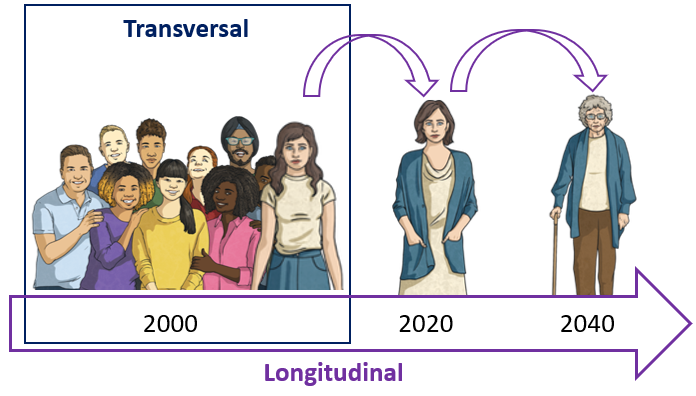
\includegraphics{./img/cap_transversal_longitudinal.png}

A realização de cada tipo de estudo é atrelada à pergunta a qual ele visa responder. A tabela abaixo apresenta algumas características.

\begin{longtable}[]{@{}lll@{}}
\toprule
\begin{minipage}[b]{0.31\columnwidth}\raggedright
Característica\strut
\end{minipage} & \begin{minipage}[b]{0.29\columnwidth}\raggedright
Transversal\strut
\end{minipage} & \begin{minipage}[b]{0.31\columnwidth}\raggedright
Longitudinal\strut
\end{minipage}\tabularnewline
\midrule
\endhead
\begin{minipage}[t]{0.31\columnwidth}\raggedright
Duração\strut
\end{minipage} & \begin{minipage}[t]{0.29\columnwidth}\raggedright
Um único momento.\strut
\end{minipage} & \begin{minipage}[t]{0.31\columnwidth}\raggedright
Múltiplos momentos.\strut
\end{minipage}\tabularnewline
\begin{minipage}[t]{0.31\columnwidth}\raggedright
Amostra\strut
\end{minipage} & \begin{minipage}[t]{0.29\columnwidth}\raggedright
Varia em cada estudo.\strut
\end{minipage} & \begin{minipage}[t]{0.31\columnwidth}\raggedright
Mesmos participantes.\strut
\end{minipage}\tabularnewline
\begin{minipage}[t]{0.31\columnwidth}\raggedright
Resultados\strut
\end{minipage} & \begin{minipage}[t]{0.29\columnwidth}\raggedright
Mostram uma fotografia momentãnea\strut
\end{minipage} & \begin{minipage}[t]{0.31\columnwidth}\raggedright
Indicam detalhes da mudança das variáveis.\strut
\end{minipage}\tabularnewline
\begin{minipage}[t]{0.31\columnwidth}\raggedright
Vantagens\strut
\end{minipage} & \begin{minipage}[t]{0.29\columnwidth}\raggedright
- Tende a ser mais barata.-Rápida.-Participantes são mais fáceis de serem amostrados.- Menos condições burocráticas (Comissão ética, etc).\strut
\end{minipage} & \begin{minipage}[t]{0.31\columnwidth}\raggedright
-Mudanças podem ser descritas.-Maior detalhamento dos resultados.-Pode indicar causalidade\strut
\end{minipage}\tabularnewline
\begin{minipage}[t]{0.31\columnwidth}\raggedright
Desvantagens\strut
\end{minipage} & \begin{minipage}[t]{0.29\columnwidth}\raggedright
-Pouco nível de detalhamento.-Impossibilidade de analisar mudanças.-Dificuldade de verificar aspectos de causalidade.\strut
\end{minipage} & \begin{minipage}[t]{0.31\columnwidth}\raggedright
-Consome tempo e dinheiro para execução.-Perda amostral tende a ocorrer com frequência.-Maior burocracia (Comissão ética, etc).-Definição de intervalo de tempo difícil.\strut
\end{minipage}\tabularnewline
\bottomrule
\end{longtable}

Com regularidade, pesquisas longitudinais se aproximam mais de objetivos (ou nível) explicativos, enquanto pesquisas transversais são mais próximas a objetivos exploratórios e descritivos.

\hypertarget{conceitos-fundamentais}{%
\section{conceitos fundamentais}\label{conceitos-fundamentais}}

\begin{itemize}
\tightlist
\item
  \emph{L. Anunciação \& J. Landeira-Fernandez}
\end{itemize}

Existem alguns conceitos muito utilizados em pesquisa e estatística que servem como fundações da maior parte dos métodos e técnicas implementados quando se deseja investigar um determinado fenômeno ou objeto através do método científico. Apesar de manuais técnicos divergirem em quantos e quais conceitos podem ser entendidos como fundamentais em pesquisa e estatística, existe grande concordância em relação à (1) realidade e modelo e (2) constante e variáveis. Ambos serão introduzidos a seguir.

\hypertarget{modelos-cientuxedficos}{%
\subsection{Modelos científicos}\label{modelos-cientuxedficos}}

Quando uma pesquisa é feita, ela visa responder uma pergunta específica sobre um fenômeno ou objeto, tal como apresentado anteriormente. Muitas perguntas são possíveis a depender da área de interesse do investigador, bem como de sua época. Físicos e astrônomos do século XVI queriam investigar a organização do sistema solar, economistas do século XVIII tinham interesse em investigar a relação entre recursos e rendimentos financeiros e, mais recentemente, psicólogos do século XX se debruçaram a estudar o efeito da escolaridade no desenvolvimento de habilidades cognitivas. Esses três exemplos remontam à teoria heliocêntrica, a lei dos retornos marginais decrescentes e a teoria da reserva cognitiva.

Apesar da diferença entre os interesses, uma característica compartilhada nestas pesquisas é a impossibilidade ou improbabilidade de se investigar diretamente a realidade. No exemplo da astronomia isso parece ser bastante claro, já que mesmo que pesquisas em física tenham características mais mecanicistas, só atualmente que o acesso mais preciso da realidade foi possível e permitiu responder melhor essa questão. Além disso, na grande maioria das pesquisas, os fenômenos e objetos de interesse não são sistemas fechados. Isso significa que não é possível ou viável controlar todos os fatores relacionados ao que se tem interesse de estudar. Por exemplo, quando se investiga como a escolaridade impacta nas habilidades cognitivas, os resultados podem (ou não) responder apenas inicialmente sobre um dos fatores relacionado às habilidades cognitivas, mas não todos.

Entre as maneiras desenvolvidas por cientistas para lidar com esta situação estão a construção de modelos teóricos e instrumentos de medida. Modelos teóricos científicos são representações da realidade e podem ser criados sob perspectiva visual, matemática, computacional ou experimental \citep{Weisberg2013}. Eles tendem a ser sistemas fechados e visam reproduzir, precisamente, o fenômeno ou objeto de interesse. A qualidade desses modelos pode variar e entre as principais características positivas de um modelo com alta aderência à realidade estão a possibilidade de se realizar simulações e também fazer predições com ele \citep{Heidemann2016}.

A figura a seguir apresenta algumas características dos modelos científicos.

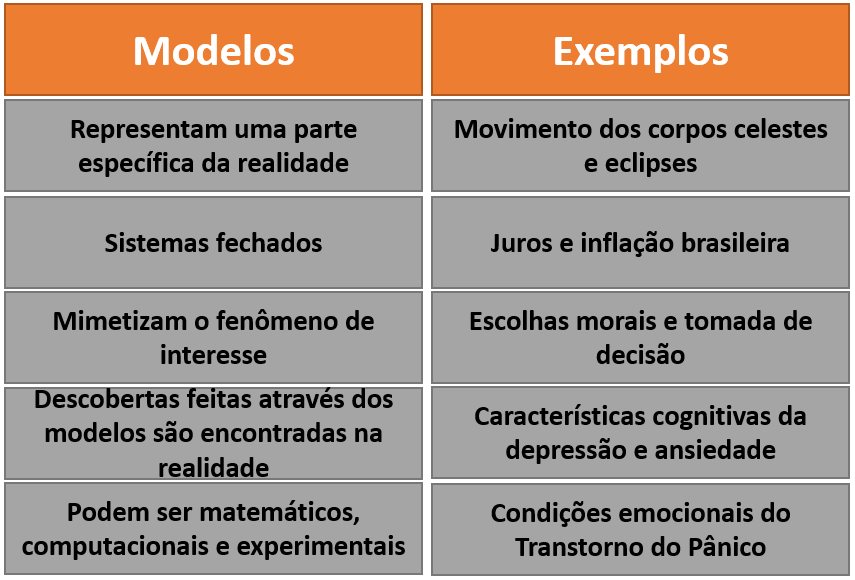
\includegraphics{./img/cap_modelos_cientificos.png}

Em um modelo ideal, aquilo que fosse descoberto a partir dele, ocorreria identicamente na realidade. Evidentemente, modelos ideais não existem na grande maioria das áreas científicas, o que leva à conclusão de que os modelos são absolutamente essenciais à pesquisa, apesar de possuírem limitações \citep{Putnam1980, Feigelson1992, Firgg2020}. Por exemplo, engenheiros utilizam modelos computacionais com muita frequência para verificar itens de segurança de um carro; economistas utilizam modelos matemáticos (e também jogos!) para investigar características da tomada de decisão e psicólogos utilizam modelos experimentais e matemáticos para investigar transtornos mentais e desenvolvimento de funções emocionais e cognitivas.

Ainda neste sentido, mapas cartográficos ilustram bem a importância dos modelos. Apesar de todos os mapas disponíveis distorcerem um pouco a área e localização dos continentes, a utilização deles é fundamental tanto na ciência como no dia-a-dia das pessoas. Na figura a seguir, o mapa à esquerda apresenta a projeção de Marcator, que é a mais utilizada nos livros. À direta, a projeção de Peters, que apesar de não ser tão utilizada, é a que melhor organiza o tamanho e o local dos continentes.

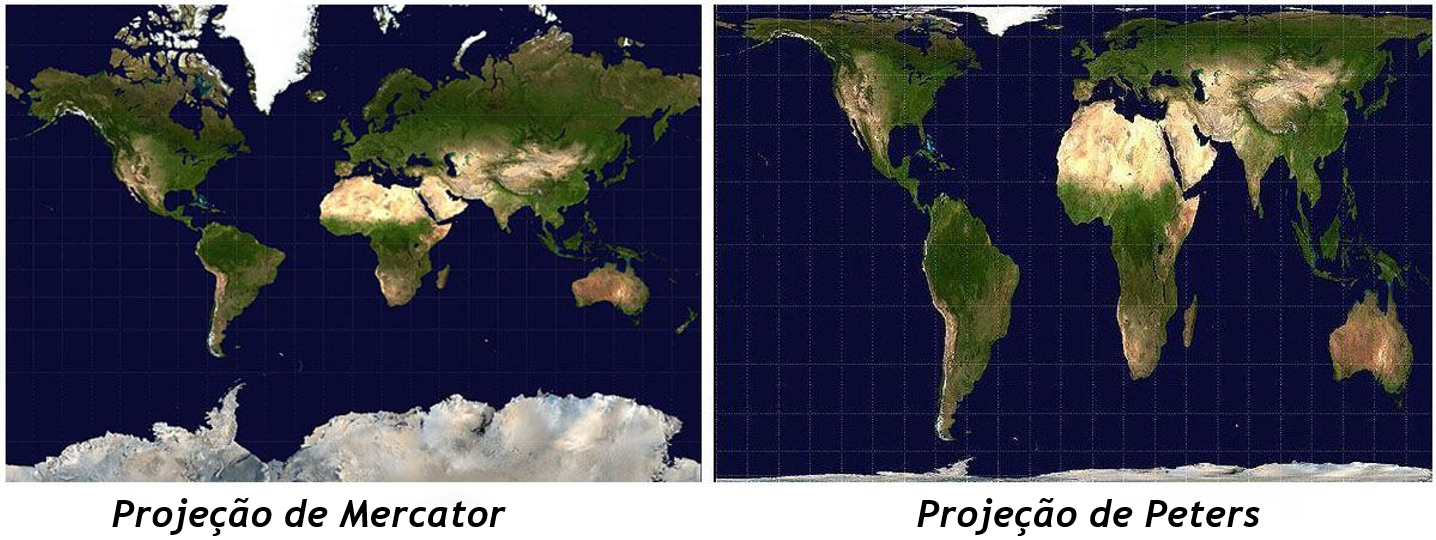
\includegraphics{./img/cap_mapas.png}

Além disso, quase sempre, o registro que temos da realidade é baseado em nossos órgãos sensoriais que, por sua vez, são influenciados pela cultura em que estamos inseridos e pela aprendizagem prévia pela qual passamos. Com isso é fácil notar que existe um grande hiato entre a realidade e nossa percepção da realidade. Os instrumentos de medida, por sua vez, são recursos tecnológicos que permitem uma avaliação mais detalhada do fenômeno ou do objeto de investigação, além de gerarem dados que podem ser analisados, comparados e compartilhados. Todas as áreas científicas criam e refinam instrumentos de medida e há autores que sugerem que a existência e a qualidade de tais recursos indicam o quão madura e desenvolvida uma área se encontra, uma vez que os instrumentos são condições centrais no processo científico \citep{Bergenholtz2018}. Apesar de grande variabilidade em relação à acurácia e precisão dos instrumentos, relógios, bússolas, réguas e testes psicológicos permitem um acesso mais detalhado de um fenômeno ou objeto de interesse.

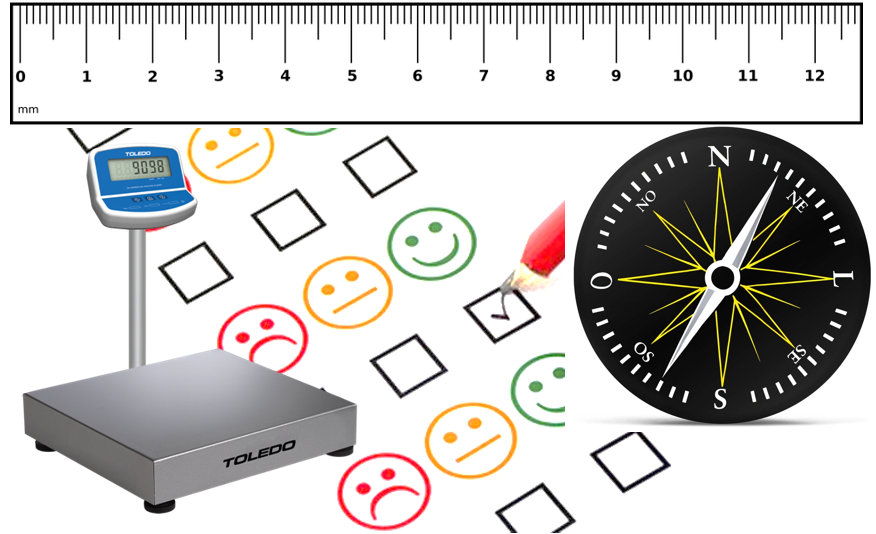
\includegraphics{./img/cap_instrumentos.png}

Dessa maneira, a principal proposta dos instrumentos de medida é a captura da realidade sem interferência ou ruídos e, em seguida, a produção de dados confiáveis sobre o fenômeno ou objeto estudado. Existe uma grande translação entre modelos teóricos e instrumentos de medida. Apesar de não ser uma regra geral, muitas áreas científicas primeiro constroem modelos teóricos e o processo de medida ocorre nestes modelos. Por exemplo, há um conjunto de modelos psicológicos visando entender como ocorre o esquecimento que, por sua vez, permitiram desenvolver testes e escalas específicas para isso.

Um dos exemplos mais interessantes sobre a limitação que nossos sentidos possuem ao capturar a realidade e a importância do desenvolvimento de instrumentos de medida é percepção que temos do sol. A maioria das representações feitas do sol o apresentam como amarelo, quando na verdade ele é branco. Isso ocorre em função da atmosfera do planeta Terra e de diferentes gases presentes no céu.

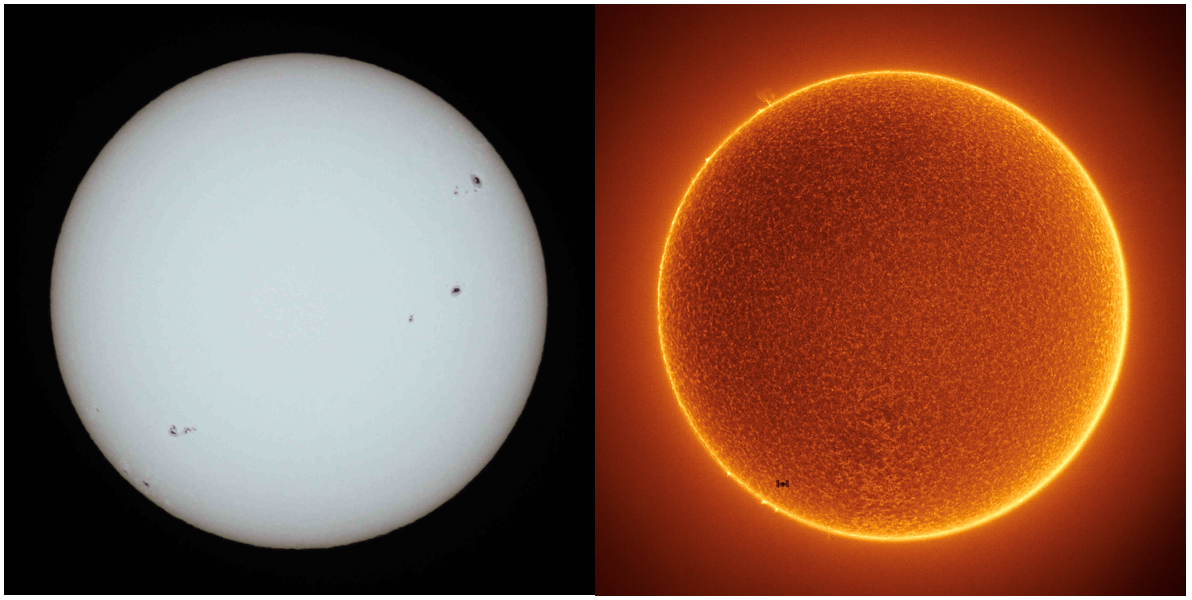
\includegraphics{./img/cap_sol.png}

Isso posto, o desenvolvimento de modelos teóricos e de instrumentos de medida são atividades essenciais de pesquisadores e cientistas para lidar com a impossibilidade ou improbabilidade de acessar a realidade de forma direta, bem como pela limitação perceptual que temos. Como Popper comenta no livro ``Os dois problemas fundamentais da teoria do conhecimento'', essas características fazem com que cientistas quase nunca digam que estão em busca da verdade, mas sim que estão em busca de evidências sobre um determinado fenômeno ou objeto.

\hypertarget{variuxe1veis}{%
\subsection{Variáveis}\label{variuxe1veis}}

O segundo conceito fundamental pode ser entendido pela dicotomia entre variáveis e constantes. De maneira geral, um fenômeno constante não apresenta dispersão em seus valores. Basta uma única medição para que o comportamento de um fenômeno constante possa ser capturado. Em oposição, fenômenos variáveis podem assumir quaisquer valores em suas características. Enquanto a velocidade da luz e do som é, respectivamente, 324 m/s e 299.792 m/s; a renda, altura ou inteligência das pessoas pode variar bastante. Essa dicotomia poderia também ser vista pelo conceito de modelos determinísticos e probabilísticos ou, superficialmente, em diferenças entre ciências naturais e ciências humanas. Modelos determinísticos são aqueles que as condições iniciais determinam os resultados, enquanto modelos probabilísticos são os que associam probabilidades aos resultados. Em ciências naturais recorre-se menos à noção de probabilidade, enquanto em ciências humanas este é um conceito central.

Em estatística e pesquisa, o termo variável pode ser entendido tanto de uma maneira bastante informal, como de uma forma mais rigorosa. Informalmente, uma variável é um símbolo que representa uma característica de um determinado objeto, tal como peso, altura, inteligência ou renda. Como essa característica pode apresentar quaisquer, dá-se o nome de variável. No entanto, formalmente em estatística, quando o termo variável é utilizado, o que está em jogo é o conceito de variável aleatória. Por sua vez, este conceito se refere à uma classe de variáveis em que o conjunto possível de suas realizações (ou seja, seus valores ou desfechos) ocorrem de acordo com uma distribuição de probabilidade \citep{everitt2002cambridge}. Em estatística, uma variável aleatória é uma função que associa elementos do espaço amostral ao conjunto de números reais.

\textbf{Atenção}: Uma variável é um símbolo que representa uma característica. Uma variável aleatória é uma variável que possui uma distribuição de probabilidade.

Dessa maneira, o estudo das variáveis (aleatórias) é central em estatística, seja tanto para análises descritiva, como inferenciais.

As variáveis podem ser organizadas por seu relacionamento em uma pesquisa, seu nível ou escala de medida e sua capacidade informacional.

No que se refere ao relacionamento entre as variáveis, inicialmente, é possível classificá-las em independentes e dependentes. Variáveis independentes são abreviadas pela sigla VI e também são chamadas de antecedentes, preditores, fatores ou variáveis manipuladas ou de entrada. Variáveis dependentes são abreviadas por VD e também são chamadas de consequentes, previstas, desfechos ou variáveis medidas ou de saída.

Os termos VI e VD explicitam que ambas as variáveis são conectadas e que a VI gera ou causa a VD. É justamente por isso que representações matemáticas apresentam a VI por X e a VD por Y, tal como no estudo de funções.

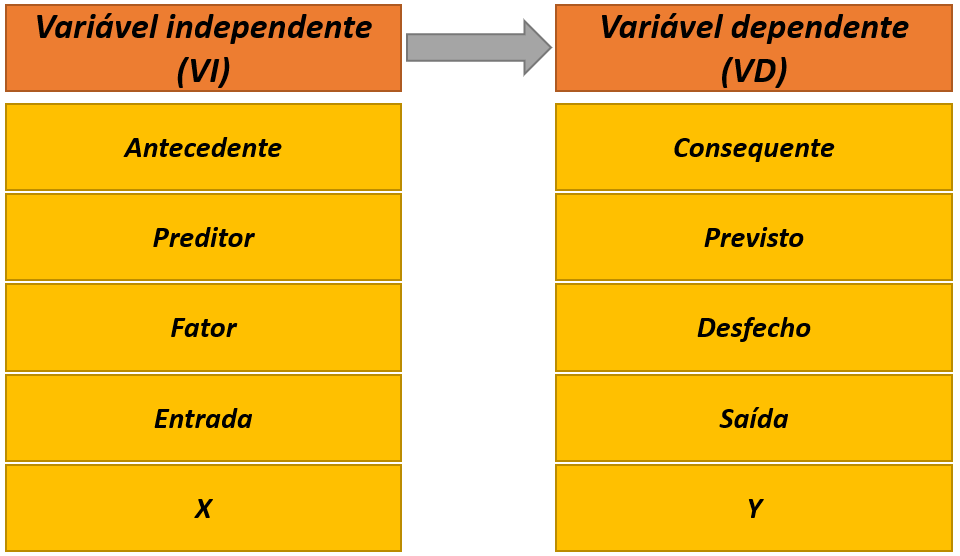
\includegraphics{./img/cap_vi_vd1.png}

Em alguns fenômenos naturais, é relativamente fácil identificar a VI e a VD. Por exemplo, quanto mais profundo uma pessoa mergulha no mar, mais gelada a água fica. Neste caso, a profundidade seria a VI, enquanto a temperatura da água seria a VD. Da mesma forma, quanto mais alto um avião viaja, menor é a pressão atmosférica. Nesse outro exemplo, a altitude é a VI e a pressão atmosférica é a VD.

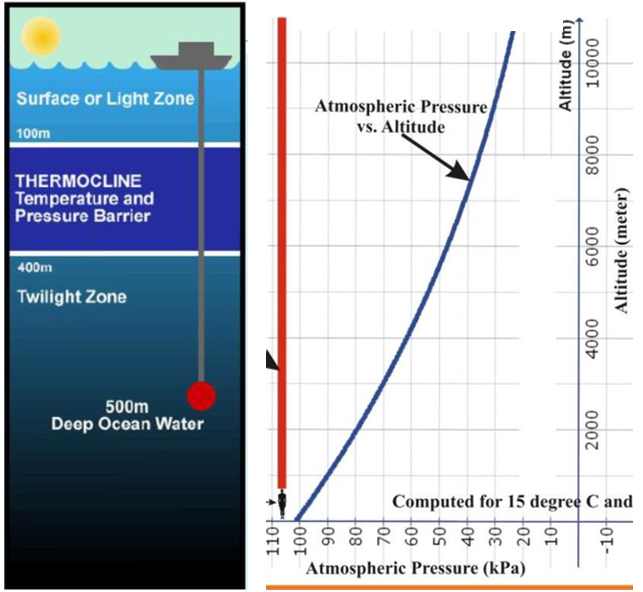
\includegraphics{./img/cap_vivd_fisica.png}

No entanto, esses exemplos descritos são oportunos e têm apenas finalidade pedagógica. Na realidade, a definição de VI e VD nem sempre é fácil e, especialmente em ciências humanas e da saúde, isso se torna ainda mais sutil. É possível definir a VI e VD por condições temporais, lógicas ou teóricas \citep{BabbieEarlR1990}, bem como é possível desenvolver pesquisas com características específicas para que essa relação possa ser definida com acurácia, e consequentemente, corretamente medida.

Como exemplos de uma condição temporal, uma pessoa pode estar interessada em investigar a influência do sexo (VI) na escolha profissional (VD) ou o efeito de um medicamento (VI) na dor de cabeça (VD). Nesses dois casos, os efeitos não podem alterar as causas. Uma escolha profissional não faz com que a pessoa altere seu sexo, bem como a dor de cabeça é uma condição que antecede a tomada do medicamento.

Em relação à condição lógica (as vezes chamada de quase-temporal), é possível que alguém queira investigar como a escolaridade afeta o preconceito. Neste caso, é viável assumir que a escolaridade é a VI e o preconceito é a VD. Entretanto, alguém pode sugerir que pessoas mais ou menos preconceituosas se dedicam de maneira diferente em atividades acadêmicas, invertendo essa relação de causalidade.

Finalmente, uma organização teórica ocorre quando se pretende investigar os efeitos da ansiedade na depressão ou do casamento no bem estar pessoal. A eleição da ansiedade como VI foi uma escolha do pesquisador e não, necessariamente, uma condição temporal ou lógica. Da mesma forma, eleger o casamento como VI é uma escolha feita para responder a uma determinada questão.

A figura a seguir traz um diagrama inicial destes conceitos, utilizando um esquema em que as horas de estudo teriam efeito sobre a nota da prova.

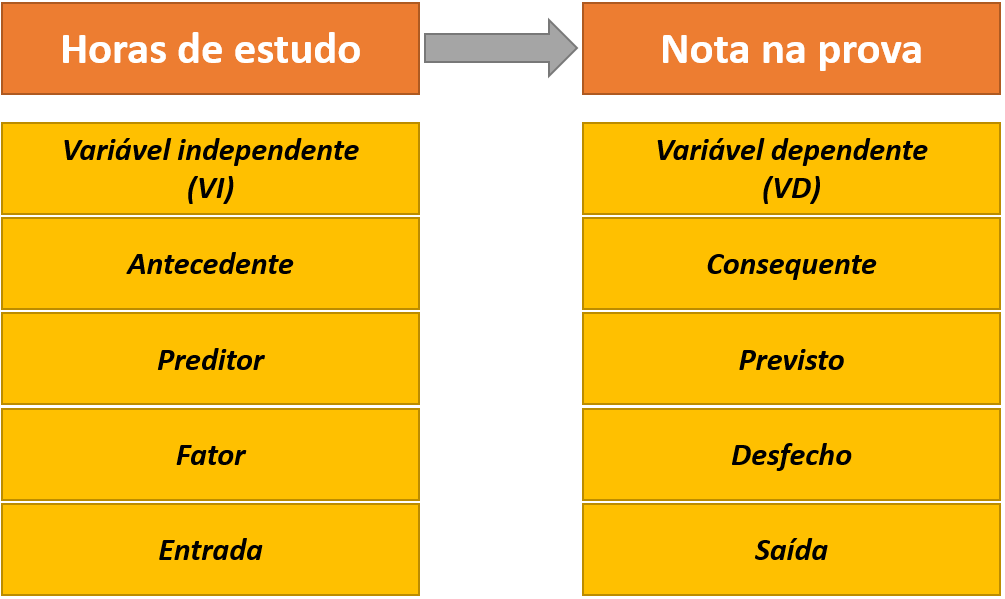
\includegraphics{./img/cap_vi_vd.png}

É importante notar que a ideia de uma única variável impactando ou causando diretamente uma outra variável é quase metafórica. Para que isso pudesse ocorrer tanto em fenômenos físicos como em quaisquer outros, seria necessário que todas as possíveis fontes de influência existentes neste relacionamento fossem controladas ou suprimidas \citep{Dumsday2012}. Essa noção de controle total é vista pelo termo \emph{ceteris paribus}, que é uma expressão em latim que significa ``tudo o mais constante''. Muitas vezes, em pesquisa e estatística, este termo é utilizado quando alguns ajustes são implementados em modelos estatísticos para tentar expressar a ideia de uma causalidade parcial, em que a VI impactaria a VD de uma determinada forma, caso tudo o mais fosse controlado \citep{Fennell2005}. Evidentemente, há fenômenos sociais que parecem obedecer à certa regularidade e o termo ``fato estilizado'' tende a ser empregado nestas situações \citep{Hirschman2016}.

Ao se pensar nas condições em que a VI e VD estejam definidas, é fácil notar que existe um conjunto grande de outras variáveis que podem impactar neste relacionamento. Essas variáveis recebem muitos nomes e o termo variáveis estranhas (VEs) pode servir para designá-las. A imagem a seguir ilustra algumas das variáveis que poderiam impactar na relação entre horas de estudo e notas na prova, previamente assumidas como VI e VD.

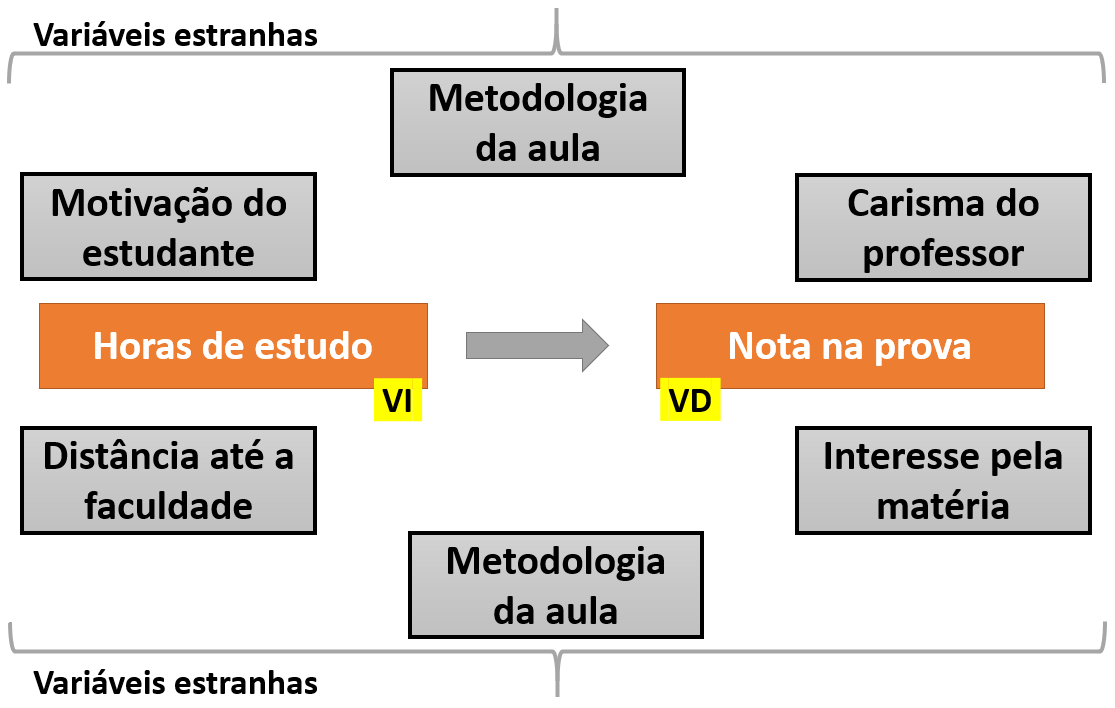
\includegraphics{./img/cap_variavel_estranha.png}

É possível afirmar que em todos os relacionamentos entre duas variáveis, sempre haverá um conjunto de outras variáveis impactando nesta relação. justamente por isso é que cientistas quase nunca digam que estão absolutamente certos de uma determinada condição ou assunto. Na maioria das vezes, como também ilustrado por Popper no livro ``Os dois problemas fundamentais da teoria do conhecimento'', cientistas tendem a substituir a palavra certeza por probabilidade.

Para conseguir mapear adequadamente o quanto e como outras variáveis impactam no relacionamento VI-VD em um estudo, é necessário ter claro o objetivo que a pesquisa possui, mas também o delineamento implementado para sua execução, o que será descrito a seguir.

\hypertarget{delineamentos-de-pesquisa}{%
\subsection{Delineamentos de pesquisa}\label{delineamentos-de-pesquisa}}

O termo delineamento diz respeito a etapa de planejamento de pesquisa em que se ``considera o ambiente em que são coletados os dados e as formas de controle das variáveis envolvidas'' \citep{gil2002}. Dessa forma, o delineamento funciona como um manual técnico. É durante esta etapa que o pesquisador terá a oportunidade de eleger as maneiras pelas quais ele irá executar seu estudo e mapear as principais características e limitações existentes.

Existem diferentes classificações dos delineamentos de pesquisa e cada área tem particularidades. É importante atentar que definir claramente o tipo de delineamento é essencial, já que os objetivos da pesquisa e as análises estatísticas a serem feitas são conectadas a ele. Em Psicologia, costuma-se organizar os delineamentos em observacionais, correlacionais e experimentais. As vezes, o termo delineamento descritivo é utilizado em vez de observacional \citep{stangor2010}. Por sua vez, em epidemiologia, saúde pública e bioestatística, os delineamentos costumam ser divididos em experimentais e observacionais \citep{friis2013, glantz2014}. Apesar das diferenças de nomenclaturas, a lógica por detrás dos delineamentos é bastante atrelada à possibilidade e viabilidade de uma manipulação ativa da VI.

Em Psicologia, a tabela abaixo é bastante utilizada:

\begin{longtable}[]{@{}llll@{}}
\toprule
\begin{minipage}[b]{0.22\columnwidth}\raggedright
Delineamento\strut
\end{minipage} & \begin{minipage}[b]{0.22\columnwidth}\raggedright
Característica\strut
\end{minipage} & \begin{minipage}[b]{0.22\columnwidth}\raggedright
Vantagens\strut
\end{minipage} & \begin{minipage}[b]{0.22\columnwidth}\raggedright
Limitações\strut
\end{minipage}\tabularnewline
\midrule
\endhead
\begin{minipage}[t]{0.22\columnwidth}\raggedright
Observacional\strut
\end{minipage} & \begin{minipage}[t]{0.22\columnwidth}\raggedright
-Apenas 1 grupo é necessário.-Descrever um determinado fenômeno ou objeto.\strut
\end{minipage} & \begin{minipage}[t]{0.22\columnwidth}\raggedright
-Oferece uma foto de um objeto ou fenômeno que tende a ser precisa.-Permite que novos estudos sejam conduzidos.-Tende a ser mais barato do que outros delineamentos.-As vezes, só é possível fazer este delineamento.\strut
\end{minipage} & \begin{minipage}[t]{0.22\columnwidth}\raggedright
-Não acessa o relacionamento entre duas ou mais variáveis.\strut
\end{minipage}\tabularnewline
\begin{minipage}[t]{0.22\columnwidth}\raggedright
Correlacional\strut
\end{minipage} & \begin{minipage}[t]{0.22\columnwidth}\raggedright
-Apenas 1 grupo é necessário.-Permite estudar a natureza e a força do relacionamento entre duas variáveis.-As vezes, só é possível fazer este delineamento.\strut
\end{minipage} & \begin{minipage}[t]{0.22\columnwidth}\raggedright
-É possível testar hipóteses sobre este relacionamento e fazer previsões de resultados futuros.-Não é necessário ambientes ou intervenções específicas.\strut
\end{minipage} & \begin{minipage}[t]{0.22\columnwidth}\raggedright
-Não permite indicar causalidade entre os fenômenos ou objetos estudados.\strut
\end{minipage}\tabularnewline
\begin{minipage}[t]{0.22\columnwidth}\raggedright
Experimental\strut
\end{minipage} & \begin{minipage}[t]{0.22\columnwidth}\raggedright
-São necessários 2 grupos em que os participantes sejam alocados de maneira aleatória.-Existe uma manipulação intencional da VI-nem participantes nem pesquisadores sabem quem está em cada grupo (duplo cego).\strut
\end{minipage} & \begin{minipage}[t]{0.22\columnwidth}\raggedright
-A aleatorização evita que as variáveis estranhas gerem vieses.-A aleatorização aumenta a probabilidade de ambos os grupos terem participantes com características similares-A comparação entre os grupos permite conclusões sobre causalidade, se assumidas algumas condições.\strut
\end{minipage} & \begin{minipage}[t]{0.22\columnwidth}\raggedright
-Impossível, impraticável ou até mesmo antiético em algumas situações, especialmente as clínicas.-O custo envolvido costuma ser alto.-O tamanho amostral tende a ser pequeno.-Há uma baixa possibilidade de generalização em pesquisas laboratoriais.\strut
\end{minipage}\tabularnewline
\bottomrule
\end{longtable}

Em Epidemiologia, saúde pública e bioestatística, costuma-se unir o delineamento observacional e correlacional. Assim, apenas os delineamentos observacional e experimental são definidos, apesar de características virtualmente similares. Pessoalmente, acredito que esta definição evita alguns equívocos, como o de achar que em delineamentos observacionais não é possível realizar correlações ou comparações entre grupos.

Todos os delineamentos possuem características específicas e um conjunto de vantagens e limitações, que serão apresentadas a seguir.

\hypertarget{delineamentos-observacionais-e-correlacionais}{%
\subsection{Delineamentos observacionais (e correlacionais)}\label{delineamentos-observacionais-e-correlacionais}}

Em delineamentos observacionais (ou observacionais e correlacionais), o pesquisador não intervém nos fenômenos estudados. Ou seja, não há uma manipulação da VI. Estudos que utilizam tal delineamento quase sempre contam com um único grupo e os resultados produzidos auxiliam no entendimento inicial do fenômeno interesse, bem como podem indicar o perfil de relacionamento entre variáveis.

Uma vez que não há a formação de grupos específicos seguindo um rigoroso controle da VI, o pesquisador deve mapear adequadamente todas as possíveis variáveis estranhas presentes no relacionamento entre VI e VD antes da pesquisa. Assim, na etapa de coleta de dados, ele poderá acessar essas variáveis para, futuramente, implementar controles estatísticos que reduzam distorções que este delineamento gera nos dados. Por exemplo, quando artigos biomédicos comentam que os resultados de um medicamento são efetivos para os participantes, controlando pela idade e sexo, essa conclusão é bem próxima de resultados obtidos por pesquisas cujos delineamentos foram observacionais.

\textbf{Atenção}: Em delineamentos observacionais, o mapeamento e acesso de variáveis estranhas auxiliam o pesquisador a implementar técnicas estatísticas que reduzam as distorções que este delineamento costuma produzir aos dados.

Nota-se que, apesar de diversas técnicas estatísticas serem utilizadas neste delineamento, não é possível falar sobre relação de causa e efeito. Apesar desta limitação, há muitas situações em que apenas este delineamento é possível. Por exemplo, estudar os impactos de um desastre natural (furacão, terremoto, etc) na percepção de segurança das pessoas, avaliar o comportamento de grupos em instituições totais, como prisões e hospícios ou as condições relacionadas ao aleitamento materno.

Uma vez que as eventuais variáveis estranhas foram previamente acessadas durante a coleta de dados, elas deixam de ser estranhas e tornam-se variáveis passíveis de análises A natureza e o local em que essas variáveis impactam no relacionamento entre a VI e a VD indicam se elas serão classificadas como intervenientes, mediadoras ou moderadoras \citep{Rooney2019, hayes2013}.

O termo variável interveniente é bastante circunscrito à Psicologia. Ele tende a ser empregado para caracterizar condições psicológicas, como motivação ou neuroticismo. Assim, este é o termo empregado quando as variáveis estranhas são fatores psicológicos.

Quando esta variável é uma consequência da VI e também impacta a VD, o termo variável mediadora costuma ser empregado. Por exemplo, ao se investigar a relação entre idade (VI) e acidentes de trânsito (VD), pode-se sugerir que pessoas mais velhas tendem a apresentar menor capacidade visual. Por sua vez, essa limitação visual pode gerar acidentes de trânsito \citep{Rhodes2011}. Neste sentido, a variável ``capacidade visual'' é uma variável mediadora.

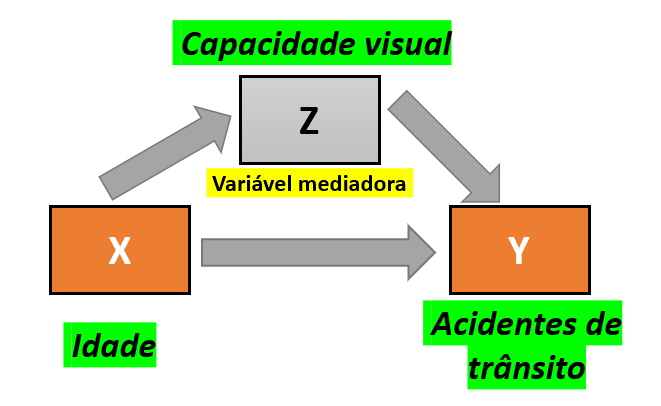
\includegraphics{./img/cap_mediacao.png}

Quando esta variável interfere no relacionamento entre a VI e a VD, podendo alterar sua natureza e intensidade, mas não é gerada pela VI, o termo variável moderadora pode ser utilizado. Por exemplo, a relação entre a satisfação de um cliente (X) e sua lealdade à marca (Y) é moderada pela sua renda \citep{Sugianto2017}. Pessoas muito satisfeitas com um produto podem ser mais ou menos leais à marca a depender de sua renda disponível.

A relação entre horas trabalhadas (X) e quantidade de produção (Y) é moderada pela qualidade do equipamento utilizado. É possível que alguém gaste muitas horas de trabalho, mas não consiga produzir absolutamente nada, se os equipamentos disponíveis funcionarem de maneira irregular. Com frequência, médicos sugerem que ao tomar medicamentos antigripais, não se deve ingerir álcool. Nesse sentido, os efeitos do medicamento (X) nos sintomas da gripe (Y) podem inclusive ser opostos em função do álcool, que age de forma moderadora.

No exemplo prévio sobre o efeito da idade (X) em acidentes de trânsito (Y), sabe-se hoje que o sexo se comporta como uma variável moderadora neste relacionamento. A literatura indica que pessoas mais novas, quando homens, tem uma alta probabilidade de se envolverem em acidentes de trânsito, especialmente os mais intensos ou graves \citep{Amarasingha2014, PRB2006}.

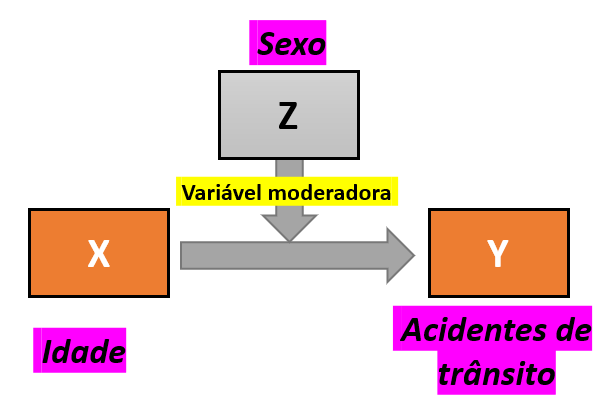
\includegraphics{./img/cap_moderacao.png}

Finalmente, é também possível identificar variáveis estranhas que interfiram tanto na VI como na VD, mas que não foram previamente mapeadas ou acessadas durante a coleta de dados. Nestes casos, é típico chamá-las de ``terceira variável'' ou ``variável de confundimento'', bem como chamar a relação entre VI e VD de ``espúria''. Por exemplo, existe uma alta correlação entre venda de sorvete (X) e morte por mordida de tubarão (Y). No entanto, essa é uma relação espúria, uma vez que é a variável ``temperatura'' que impacta tanto na VI como na VD. Da mesma maneira, existe uma alta correlação entre quantidade de bares e igrejas nas cidades, mas ambos os fenômenos são explicados pela densidade populacional do local.

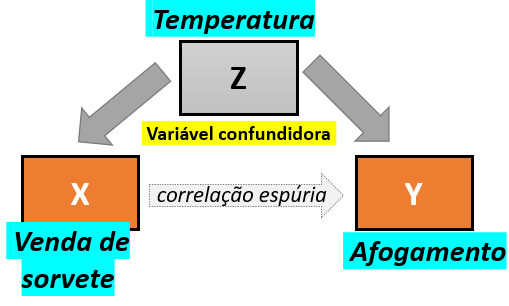
\includegraphics{./img/cap_confundimento.png}

Talvez quando mais novo(a), alguém tenha lhe dito que as cegonhas traziam os bebês. Isso não é verdade, apesar de ser um ótimo exemplo de variável de confundimento. A relação entre número de ninhos de cegonha (X) e número de bebes nascidos (Y) é confundida pela temperatura do local 9 meses atrás \citep{Matthews2000}. Cegonhas e seres humanos têm seus filhos ou filhotes na mesma época. Curiosamente, como as cegonhas por vezes constroem seus ninhos em telhados de casas, especialmente as com chaminés por conta do calor, as pessoas acreditavam que se uma cegonha fizesse o ninho em seu telhado, isso indicaria que o casal iria ter um filho. Em alguns países, se achava também que deixar doces na janela seria uma maneira de informar as cegonhas que a casa estava pronta para ter um bebê.

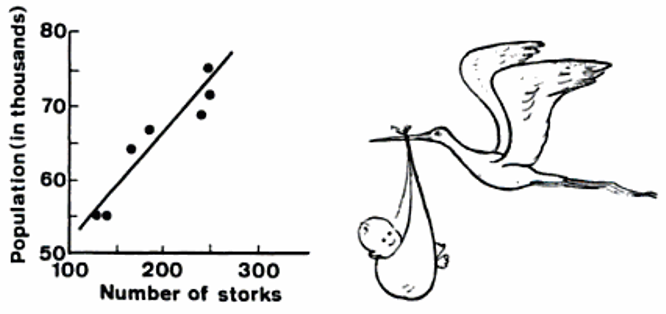
\includegraphics{./img/cap_cegonha.png}

A literatura é bastante rica de exemplos para tais condições, mas também de discussões e debates acadêmicos sobre esses conceitos. A tabela a seguir reúne esforços e exemplifica onde tais conceitos são implementados.

\begin{longtable}[]{@{}ll@{}}
\toprule
\begin{minipage}[b]{0.10\columnwidth}\raggedright
Relacionamento\strut
\end{minipage} & \begin{minipage}[b]{0.84\columnwidth}\raggedright
Exemplo\strut
\end{minipage}\tabularnewline
\midrule
\endhead
\begin{minipage}[t]{0.10\columnwidth}\raggedright
Moderação\strut
\end{minipage} & \begin{minipage}[t]{0.84\columnwidth}\raggedright
Relação entre ansiedade (X) e performance (Y), o tipo de atividade poderia ser uma variável moderadora\strut
\end{minipage}\tabularnewline
\begin{minipage}[t]{0.10\columnwidth}\raggedright
Moderação\strut
\end{minipage} & \begin{minipage}[t]{0.84\columnwidth}\raggedright
Relação entre efeito de um remédio (X) e sintomas de resfriado (Y), a ingestão de álcool poderia ser uma variável moderadora\strut
\end{minipage}\tabularnewline
\begin{minipage}[t]{0.10\columnwidth}\raggedright
Moderação\strut
\end{minipage} & \begin{minipage}[t]{0.84\columnwidth}\raggedright
Relação entre idade (X) e problemas cognitivos (Y), a escolaridade poderia ser uma variável moderadora\strut
\end{minipage}\tabularnewline
\begin{minipage}[t]{0.10\columnwidth}\raggedright
Moderação\strut
\end{minipage} & \begin{minipage}[t]{0.84\columnwidth}\raggedright
Relação entre stress (X) e depressão(Y), o suporte social poderia ser uma variável moderadora\strut
\end{minipage}\tabularnewline
\begin{minipage}[t]{0.10\columnwidth}\raggedright
Mediação\strut
\end{minipage} & \begin{minipage}[t]{0.84\columnwidth}\raggedright
Relação entre idade (X) e uso de mídias sociais (Y), a quantidade de tempo livre pode ser mediadora\strut
\end{minipage}\tabularnewline
\begin{minipage}[t]{0.10\columnwidth}\raggedright
Mediação\strut
\end{minipage} & \begin{minipage}[t]{0.84\columnwidth}\raggedright
Relação entre quantidade de hora de trabalho (X) e desgaste (Y), o retorno financeiro poderia ser mediador\strut
\end{minipage}\tabularnewline
\begin{minipage}[t]{0.10\columnwidth}\raggedright
Mediação\strut
\end{minipage} & \begin{minipage}[t]{0.84\columnwidth}\raggedright
Relação entre conscienciosidade (X) e saúde (Y), comportamentos saudáveis poderiam ser mediadores\strut
\end{minipage}\tabularnewline
\bottomrule
\end{longtable}

\emph{Nota: A definição de variável mediadora e moderadora pode ser tornar mais difícil, como é visto no caso entre idade e problemas cognitivos, já que a escolaridade costuma depender também da idade}

Em síntese, a principal característica de estudos com delineamentos observacionais é a não manipulação da VI por parte do pesquisador.

Como outros exemplos, pode-se listar estudos em que se objetivou investigar os hábitos, práticas e produtividade de pesquisadores \citep{Wenke2017}, a alimentação durante a pandemia \citep{Amatori2020} ou aspectos epidemiológicos de transtornos mentais de universitários brasileiros, portugueses e espanhóis \citep{AfonsoJunior2020}.

\hypertarget{delineamentos-experimentais}{%
\subsection{Delineamentos experimentais}\label{delineamentos-experimentais}}

De maneira geral, delineamentos experimentais representam o melhor exemplo de uma pesquisa científica, além de serem os mais prestigiados no meio acadêmico \citep{gil2002}. Apesar destes delineamentos poderem apresentar pequenas distinções, o formato mais típico é marcado pelas seguintes características: (1) dois grupos de uma mesma população são formados de maneira aleatória, (2) deve haver uma manipulação intencional do pesquisador sobre a VI e (3) nem o participante, nem o pesquisador sabem em que grupo cada um está, o que é chamado de duplo-cego.

Cada um desses elementos confere uma propriedade importante para este delineamento. Inicialmente, a formação de dois grupos é uma condição de base deste delineamento e o diferencia de delineamentos observacionais. Nestes últimos, a composição de grupos também pode ocorrer, mas quase sempre após a coleta de dados e para responder questões estatísticas. A alocação dos participantes em ambos os grupos de maneira aleatória assegura que as variáveis estranhas terão impacto equânime em ambos os grupos, além de aumentar a probabilidade de os grupos serão formados por participantes com características similares.

A segunda característica é a atitude ativa do pesquisador. Neste delineamento, a VI será manipulada e apenas um grupo será exposto a ela, enquanto outro não. O grupo em que a VI será inserida é, tradicionalmente, chamado de experimental, enquanto o outro é chamado de controle.

Finalmente, como nem o pesquisador nem o participante sabem quem está em cada grupo, isso inibe que os participantes tentem mudar de grupo e reduzem o impacto que as expectativas do pesquisador e/ou do participante possam ter sobre os resultados.

A figura a seguir apresenta estas características.

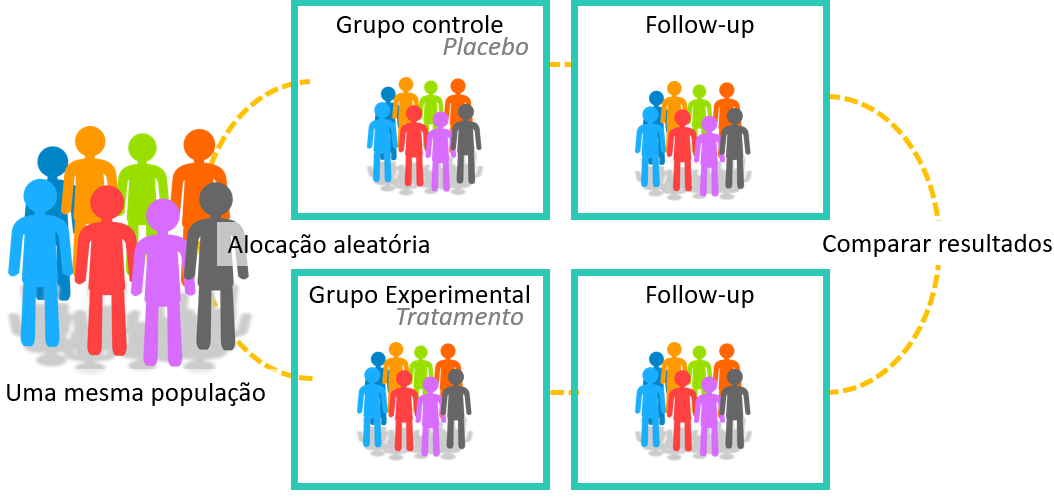
\includegraphics{./img/cap_experimento.png}

É possível notar que o delineamento experimental é, de longe, o que melhor consegue mapear as VIs, VDs, bem como controlar efetivamente as VEs. Essas vantagens dão força para resultados que visem expressar relações de causa e efeito, mas também geram muitas dificuldades. De fato, para arguir sobre causalidade, é necessário precedência temporal, eliminação de explicações alternativas, que a VI sempre esteja presente (necessidade) e que sempre impacte na VD (suficiência).

Além disso, há algumas condições que limitam ou impedem a execução deste delineamento. O custo para sua realização tende a ser bastante elevado, o tamanho amostral é frequentemente pequeno e pesquisas laboratoriais costumam reproduzir mal o cotidiano das pessoas, diminuindo a capacidade de generalização dos resultados. Para aumentar a capacidade de generalização dos resultados, por vezes, tenta-se implementar este delineamento em ambientes naturalísticos (ou ecológicos). No entanto, apesar de vantagens, isso quebra o princípio da aleatoriedade, impactando negativamente para o controle das variáveis estranhas.

Quando as pesquisas são feitas em condições clínicas, a perda e morte experimental são frequentes e muitas condições éticas emergem, impedindo a implementação deste delineamento. Por exemplo, avaliar diferentes situações em relação à amamentação materna (um grupo de mães amamenta seus filhos e outro não), o impacto de desastres naturais no comportamento das pessoas ou o efeito de mudanças abruptas legislativas e sociais na interação entre grupos retratam tal condição.

Em epidemiologia e saúde pública, este delineamento é também chamado de \emph{Randomized Controlled Trial (RCT)} ou Ensaio Clínico Randomizado. Especialmente nestas áreas, existem diversas situações em que em a VI foi selecionada em vez de manipulada. Quando isso ocorre, o delineamento passa a ser chamado de quase-experimental.

A literatura oferece bons exemplos sobre este delineamento. O psicólogo Albert Bandura \earpar{Bandura1961} teve o interesse de estudar o efeito da exposição à violência no comportamento agressivo durante a interação social de crianças e, para isso, desenvolveu um delineamento experimental. Ele dividiu as crianças em grupos específicos, em que 1 grupo via uma televisão que passava adultos agredindo um boneco João Bobo e outro via cenas neutras. Os comportamentos agressivos eram avaliados durante o momento do recreio, que ocorria imediatamente após as crianças terem visto televisão. Um grupo de psicólogos visou comparar dois programas de intervenção escolar em um grupo de 164 crianças em vulnerabilidade econômica nos EUA e, para isso, uma parte frequentou aulas de apoio e outra continuou com o ensino usual \citep{Feil2020}.
Finalmente, os economistas Redzo e Paul Frijters \earpar{Mujcic2020} quiseram verificar o efeito da cor de pele na probabilidade de receber uma carona de ônibus. Para isso, eles utilizaram um delineamento quase-experimental, em que atores pretos e brancos entravam em ônibus de uma mesma empresa e perguntavam ao motorista, de uma maneira padronizada, se poderiam viajar de graça 2 estações. A concordância ou não dos motoristas foram tabuladas e, depois, comparadas.

\hypertarget{considerauxe7uxf5es-sobre-escalas-de-medida-e-o-processo-de-mensurauxe7uxe3o-em-psicologia}{%
\section{Considerações sobre escalas de medida e o processo de mensuração em Psicologia}\label{considerauxe7uxf5es-sobre-escalas-de-medida-e-o-processo-de-mensurauxe7uxe3o-em-psicologia}}

\begin{itemize}
\tightlist
\item
  \emph{L. Anunciação \& J. Landeira-Fernandez}
\end{itemize}

A existência de um fenômeno é condicionada à uma determinada quantidade. Como atribuído à Thorndike \earpar{Thorndike1914}, ``Se algo existe, ele tem de existir em uma certa quantidade e se uma determinada quantidade existe, ela pode ser mensurada''. Assim, tal como em outras ciências, o processo de mensuração é absolutamente vital à Psicologia. Isso pode ser demonstrado tanto pela implementação de técnicas estatísticas para modelar fenômenos psicológico, como pelas lentes de uma das áreas mais voltadas ao desenvolvimento de instrumentos, que é a Psicometria. Entretanto, nunca faltaram céticos de diferentes locais questionando se fenômenos psicológicos poderiam, de fato, ser medidos e uma das primeiras e mais estáveis respostas sobre esse questionamento ocorreu em 1946, com a publicação intitulada ``On the theory of scales of measurement'' do psicólogo e psicofísico Stanley Stevens.

Este trabalho apresentou algumas conclusões que até hoje são importantes e que tocam, principalmente (1) à definição de medida, (2) o conceito de escalas (níveis) de medida e (3) à condição da mensuração de fenômenos psicológicos. Inicialmente, Stevens parafraseou N.R. Campbell ao entender que a ``mensuração, em sentido mais amplo, é definida como a atribuição de números a objetos ou eventos de acordo com algumas regras'' \citep[p.677]{Stevens1946}.

Uma vez feito isso, ele concluiu que esses números são atribuídos (ou existem) em função da possibilidade de realização de operações estatísticas e matemáticas com eles. Duas regras gerais são subjacentes neste conceito: a primeira é que a as operações possíveis para cada escala são as que se mantêm invariantes para as transformações matemáticas que cada um dos níveis de mensuração aceita e a segunda é que é necessário que haja um isomorfismo (as vezes, apresentado como s(x)) entre os entre os objetos que estão sendo medidos e os números atribuídos a eles.

Em função destas condições, Stevens descreve quatro escalas que se apresentam hierarquicamente como: (i) nominal, (ii) ordinal, (iii) intervalar e (iv) de razão. Desde o trabalho de Stevens, essa relação entre o valor numérico e o objeto para o qual este valor foi utilizado atraiu ao menos dois grupos de pesquisadores, que são aqueles que possuem um interesse mais voltado à análise de informação que este número ou esta escala traz e, neste sentido, tentam responder à pergunta ``O que este número está informando'' e os que possuem um maior interesse em desenvolver tratamentos estatísticos a tais números ou escalas e, analogamente, tentam responder à pergunta ``Como que se trata estatisticamente tais números?''.

Posto isso, esta seção realiza uma síntese deste conceito, bem como apresenta as descrições de cada uma das escalas, especialmente a partir de uma orientação mais pragmática, suas condições de uso e uma breve contextualização atual.

\hypertarget{escala-nominal}{%
\subsection{Escala nominal}\label{escala-nominal}}

Essa escala é a mais primitiva de todas e a única regra relacionada ao processo de mensuração é que o número atribuído a um determinado objeto ou evento deve ser exclusivo, não sendo possível atribuir um mesmo número a diferentes eventos ou objetos. É importante destacar que os números aqui são arbitrários e, além disso, não refletem grandezas ou magnitudes.

Nessa escala, só é possível contagens e proporções. Em relação a aspectos estatísticos, é possível obter apenas a moda dos valores. Exemplos concretos são: o número da camisa dos jogadores de futebol, atribuir o valor 1 para homens e 2 para mulheres ou 1 para psicólogos, 2 para geógrafos e 3 para pedagogos.

É importante notar existem livros e manuais que consideram que quando há apenas dois valores possíveis para o objeto ou evento, o ideal é chamar essa escala de ``dicotômica'', ``binária'' ou ``dummy'', mas isso varia bastante em função da área e o consenso não é fácil. Por exemplo, em estudos em ciências sociais, é possível encontrar autores chamando a classificação de sexo biológico (por exemplo, 1 para homens e 2 para mulheres) de variável binária; já em estudos epidemiológicos, é frequente à atribuição do valor ``1'' para um grupo de pessoas com uma determinada doença e ``0'' para um grupo de pessoas sem esta doença (apesar disso poder ser entendido como ordinal em alguns casos) e, finalmente, em estudos em economia, por vezes os pesquisadores utilizam o valor ``1'' para indicar algo de interesse (por exemplo, desempregado) e ``0'' para caso contrário.

Tirando essas particularidades, é fundamental entender que os números atribuídos à essa escala são arbitrários e apenas identificam objetos ou eventos.

\hypertarget{escala-ordinal}{%
\subsection{Escala ordinal}\label{escala-ordinal}}

Nessa escala, os números respeitam uma relação de ordem ranqueada e essa é a regra pela qual os números são atribuídos aos eventos ou objetos.

É importante ter em perspectiva que essa escala pode ser utilizada pragmaticamente em uma pesquisa mesmo quando o fenômeno que está sendo estudado é facilmente compreendido dentro de uma escala superior, como será visto. Por exemplo, é plenamente possível que um psicólogo meça o tempo de reação de um grupo de pessoas e depois tenha criado categorias ordenadas, como ``lento (1)'', ``esperado (2)'' e ``rápido (3)''. Em função disso, alguns livros tentam dividir essa escala a partir de uma origem objeto ou evento que está sendo medido e utilizam de termos como ``origem natural'' e ``origem não natural'', que não serão utilizados aqui (Pasquali, 1998).
Nessa escala, além da contagem, proporções e moda, é também possível identificar mínimo, máximo e amplitude. Exemplos concretos são a Escala de dureza dos metais (Escala de Mohs), o nível de satisfação de uma empresa, onde 1 é baixo, 2 é moderadamente satisfeito e 3 é alto e a posição ao fim de uma corrida, podendo ser o primeiro lugar, segundo ou terceiro.

\hypertarget{escala-intervalar}{%
\subsection{Escala intervalar}\label{escala-intervalar}}

Os números aqui assumem um aspecto propriamente quantitativo e, em outras palavras, quase sempre o número não segue nem uma relação arbitrária (por exemplo, 1 para homens e 2 para mulheres), nem tampouco uma convenção informal (por exemplo, 1 para ensino fundamental e 2 para ensino médio), mas é obtido a partir de um processo em que se contou com a utilização de instrumentos de medida.
Nessa escala, as distâncias entre as categorias são iguais, apesar do valor zero ser uma conveniência. Dessa maneira, a diferença entre categorias será sempre relacional e jamais absoluta. Assim, nesse nível, é possível ter propriedades aditivas, mas não multiplicativas. Considerando unidades arbitrárias, é possível falar que a diferença entre 30 e 29 (1 unidade) é a mesma que entre 15 e 14 (1 unidade). No entanto, no que diz respeito à magnitude do que está sendo medido, nessa escala não é possível falar que 30 unidades é o dobro de 15 unidades.

Nessa escala, além da contagem, proporções, moda, identificar mínimo, máximo e amplitude, é possível tirar diferenças e fazer adições, bem como calcular a média, a variância e o desvio-padrão dos resultados.
Exemplos concretos são o calendário que utilizamos. Repare que utilizamos ``AC'' (antes de Cristo) e ``DC'' depois de Cristo, estipulando um zero arbitrário; a temperatura sendo medida por graus Célsius ou Fahrenheit, já que cada uma dessas medidas tem um ponto 0 arbitrário. Aproveitando o exemplo da temperatura para ilustrar mais detalhadamente o que significa ``0'' arbitrário, o valor ``0o C'' na escala célsius se refere à temperatura que a água congela, enquanto ``100o C'' se refere à temperatura em que a água entre em ebulição. Em Fahrenheit, esse valor é o ``32 o F'' e ``212 o C''.

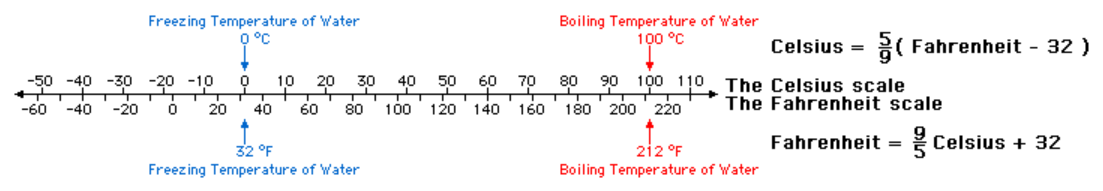
\includegraphics{./img/cap_escala_medida_farenheit1.png}

Apesar de haver a possibilidade de conversão de uma escala para outra, repare que não é possível utilizar a propriedade multiplicativa. Por exemplo, enquanto numericamente 30 x 2 = 60, afirmar que 30º C x 2 = 60º C é incorreto. Na verdade, 30º C se refere a 86º F e 60º C se refere a 140º F.

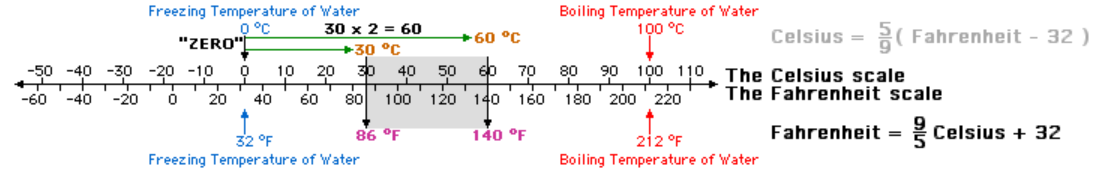
\includegraphics{./img/cap_escala_medida_farenheit2.png}

Assim, apesar de ser intuitivo pensar que se um ambiente tem 32 graus célsius, ele está o dobro de quente de um ambiente que está 16º celsius, isso não é correto.

\hypertarget{escala-de-razuxe3o}{%
\subsection{Escala de razão}\label{escala-de-razuxe3o}}

Aqui há um 0 absoluto e todas as operações previamente podem ser feitas, bem como o produto das categorias. Escalas de razão são mais encontradas na física. Nessa escala, além das capacidades matemáticas previamente descritas, é possível implementar propriedades multiplicativas. Raramente, essa escala será utilizada em um processo de avaliação psicológica. Entretanto, algumas pesquisas costumam utilizar variáveis que pertencem à escala de razão, como pesquisas em psicofísica que medem o tempo de ``tempo de reação'' ou pesquisas em neuropsicologia da atenção que medem a ``quantidade de botões apertados em um minuto''. É importante novamente alertar que mesmo que essa medida tenha um 0 absoluto (por exemplo, uma pessoa não apertou nenhum botão ao fim de um minuo), isso não significa em nada que o fenômeno psicológico subjacente seja inexistente ou ausente.

\hypertarget{suxedntese-das-caracteruxedsticas-de-cada-escala}{%
\subsection{Síntese das características de cada escala}\label{suxedntese-das-caracteruxedsticas-de-cada-escala}}

Como exposto logo ao início, os números presentes em cada uma das escalas podem ser entendidos tanto por seus aspectos de informação como pelos procedimentos estatísticos a eles associados. Ambas as iniciativas possuem sua importância e são associadas entre si. Os gráficos expostos abaixo apresentam ambos os conceitos.

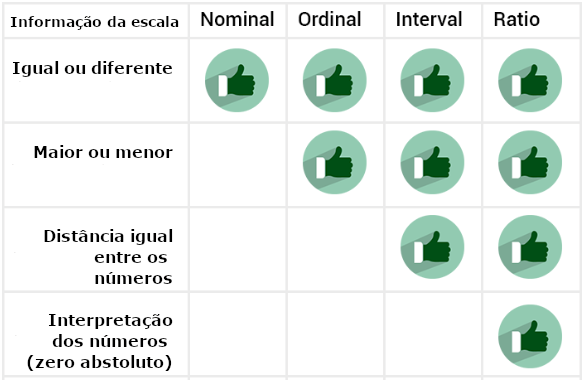
\includegraphics{./img/cap_escala_medida_informacao.png}

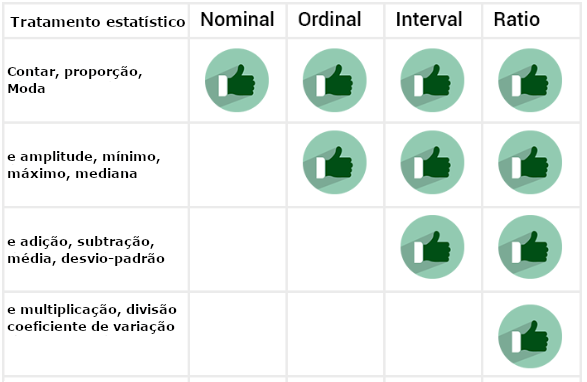
\includegraphics{./img/cap_escala_medida_analises.png}

\hypertarget{as-escalas-de-stevens-e-uma-tentativa-de-agrupamento}{%
\subsection{As escalas de Stevens e uma tentativa de agrupamento}\label{as-escalas-de-stevens-e-uma-tentativa-de-agrupamento}}

Apesar de Stevens ter, fundamentalmente, criado quatro escalas em que sempre haverá números associados a objetos a partir de sua capacidade matemática, teóricos posteriores tentaram agrupar essas quatro escalas em dois conjuntos específicos que costumam ser feitos seguindo este critério: uma vez que as escalas nominal e ordinal utilizam os números de uma maneira assegurada apenas por convenção, muitos livros e autores as agrupam como ``qualitativas''. Por contraste, como a escala intervalar e de razão são obtidas, majoritariamente, por processos que contam com instrumentos de medida, elas quase sempre são agrupadas como ``quantitativas''.

Mesmo que hoje em dia esse agrupamento seja bastante corriqueiro, origem desta iniciativa é algo incerta. Há sugestão que ela tenha começado pelo trabalho de investigação semiótica de Charles Sanders Peirce. Esse filósofo julgava que a ciência avançava em dez níveis distintos e progressivos, começando por um ícone possível (fancy), passando por um pensamento, um objeto, um símbolo numérico, uma quantidade e uma relação \citep[p.289]{smart1999}. Infelizmente, essa classificação pode gerar uma divisão desnecessária dentro do próprio conceito desenvolvido por Stevens, além de gerar bastante confusão, já que o termo ``pesquisa qualitativa'' não costuma se referir às escalas de medida, mas sim à uma área que mais recentemente emergiu com uma forma metodológica distinta e, eventualmente, até mesmo crítica às iniciativas de medida e mensuração. Além disso, o termo ``quantitativa'' atribuído apenas à escala intervalar e de razão pode dar a impressão inadequada de que não se usa números nas escalas nominais ou ordinais. Finalmente, é importante frisar que há livros que utilizam o termo ``categórica'' para ``qualitativa'' e ``propriamente numérico'' para ``quantitativa'', aumentando algo mais os cenários de confusão. A imagem a seguir apresenta esta tentativa.

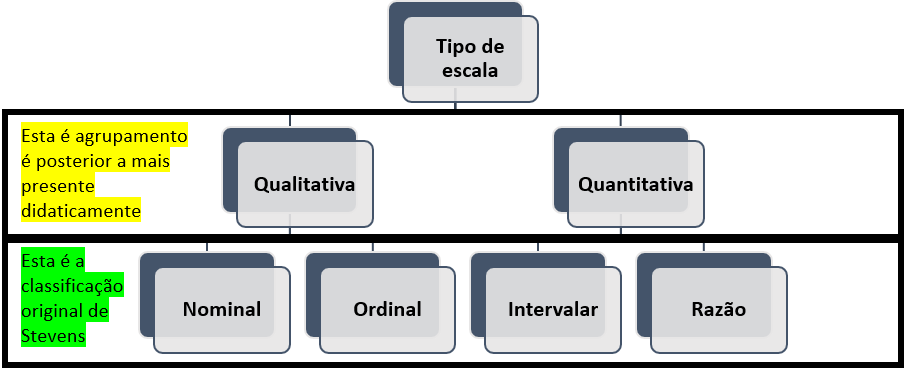
\includegraphics{./img/cap_escala_medida_agrupamento.png}

\hypertarget{variuxe1veis-discretas-ou-contuxednuas}{%
\subsection{Variáveis discretas ou contínuas}\label{variuxe1veis-discretas-ou-contuxednuas}}

A iniciativa de classificar as variáveis e, consequentemente, escalas de medida não foi apenas feita em estudos psicológicos. Evidentemente, áreas como matemática, probabilidade e estatística também tiveram (e ainda possuem) interesse em classificar as variáveis e uma das maneiras pelas quais isso é feito diz respeito à forma como os valores se apresentam, especialmente em sua capacidade informacional \citep{morettin_bussab_2010}.

Qualquer variável cujo resultado só possa descreve uma quantidade contável, em que os valores potenciais podem ser enumerados em uma ordem é chamada de discreta e é caracterizada por uma função de massa probabilidade (em inglês, probability mass function). Por sua vez, uma variável cujos valores potenciais não podem ser enumerados em uma ordem inequívoca é chamada de contínua e tem uma função de densidade de probabilidade (em inglês probability density function). Um atalho cognitivo bastante frequente apesar de apenas parcialmente correto pode auxiliar: variáveis discretas costumam ter valores inteiros, tal como número de filhos, caixas de remédios vendidas por uma farmácia e vezes que um paciente buscou auxílio médio; por sua vez, as variáveis continuar reúnem números fracionários, tal como a altura dos filhos, o retorno financeiro em Reais que a venda dos remédios e o tempo gasto em cada em cada consulta média.

Quando se tenta fazer uma comparação entre a classificação de escalas de medida desenvolvida por Stevens e a classificação das variáveis em discretas e contínuas, é possível considerar que a escala intervalar e de razão podem também ser entendidas como discretas e continuas. Excepcionalmente e apenas para fins de modelagem estatística, as variáveis classificadas como nominais e ordinais podem ser entendidas também como discreta \citep[p.20]{Borgatta1980, privitera2016}

\hypertarget{hierarquia-da-classificauxe7uxe3o-e-a-importuxe2ncia-desses-conceitos-hoje-em-dia}{%
\subsection{Hierarquia da classificação e a importância desses conceitos hoje em dia}\label{hierarquia-da-classificauxe7uxe3o-e-a-importuxe2ncia-desses-conceitos-hoje-em-dia}}

Uma vez que as escalas dependem das capacidades matemáticas associadas, uma escala de maior nível pode ser convertida em uma escala hierarquicamente inferior. Isso foi previamente apresentado na escala ordinal com o exemplo de tempo de resposta. Esse processo de transformação costuma ser chamado de ``categorização'' e pode ser facilmente visto em outros exemplos. Por exemplo, a altura das pessoas (razão, contínua) pode ser classificada em baixas ou altas e a temperatura em Kelvin (razão, contínua) pode tanto ser entendida de maneira intervalar (Celsius, por exemplo), ordinal (muito frio, frio, quente, muito quente) ou (agradável e desagradável).

Apesar dessas classificações de escalas/níveis de medida terem importância acadêmica, em situações de análise de dados, quase nunca a diferenciação entre os 4 níveis de medida tem relevância ou utilidade. Além disso, o próprio Stevens, tempos depois, em 1959, reviu algo de sua classificação e reconheceu que as regras de invariância também permitiam uma nova escala, chamada de ``log-intervalar'' \citep{stevens1959}. Essa escala quase nunca presente em livros didáticos.

Além disso, como programas estatísticos são frequentemente utilizados para realizar procedimentos de análises de dados, eventualmente eles sequer utilizam as mesmas nomenclaturas ou apenas entendem as variáveis como discretas ou contínuas. Mesmo na academia, autores como D. Howell consideram que esse aspecto da medida tem apenas relevância histórica, sendo irrelevante hoje em dia \citep[p.~18]{howell2011}.

Finalmente, a partir da tentativa de desenvolver ou aperfeiçoar o isomorfismo entre relações empíricas e relações algébricas, em que houvessem regras bem definidas articulando os números às coisas (tal como visto em Campbell), e que tivessem propriedades matemáticas específicas e bem definidas (tal como visto em Stevens) outras classificações foram surgindo. Entre eles, a Teoria representacional da medição (Patrick Suppes) e a Teoria da Medida Aditiva Conjunta (TMAC) \citep{Michell1993}.

\hypertarget{em-qual-escala-devemos-classificar-os-testes-psicoluxf3gicos}{%
\subsection{Em qual escala devemos classificar os testes psicológicos}\label{em-qual-escala-devemos-classificar-os-testes-psicoluxf3gicos}}

Psicólogos e outros cientistas comportamentais utilizam com frequência instrumentos de medida para acessar variáveis como atenção, memória, personalidade e inteligência. De maneira análoga às outras áreas empíricas, esses instrumentos geram resultados numéricos que, por sua vez, são utilizados para as mais diferentes finalidades.

Da mesma forma que para maioria dos fenômenos medidos, o nível de medida não é inerente aos dados \citep{Velleman1993}. Com isso, o debate sobre qual nível de medida devem ser entendido os números obtidos por instrumentos psicológicos parece estar sempre aberto. Uma primeira resposta veio do próprio Stevens, que assumindo que as operações possíveis em cada escala devem ser invariantes comentou que:

\begin{quote}
A maioria das escalas usadas amplamente e efetivamente por psicólogos são ordinais. De maneira estrita, médias e desvios-padrão não devem ser utilizados nessas escalas, uma vez que para essas estatísticas se deva saber algo mais do que a ordem relativa dos dados. Por outro lado, pode-se evocar uma espécie de confirmação pragmática para esse uso `ilegal' da estatística: em inúmeras situações o seu uso conduziu a resultados frutuosos (Stevens, 1946, p.~679, aspas do autor original).
\end{quote}

Já no meio acadêmico, é bem possível que ninguém consideraria que os resultados obtidos por um processo de testagem psicológica sejam nominais ou de razão. Entretanto, há bastante divergência em relação quanto ao nível ordinal ou intervalar. Excetuando os que julgam que os resultados estão entre esses dois níveis, há aqueles que julgam que a escala ordinal é a adequada para qualquer instrumento psicológico. Para esses autores, não seria possível sequer somar ou diminuir os valores obtidos em itens de um teste de inteligência ou inventário de atitude. Eventualmente, decisões como essa são bastante rígidas e só mais recentemente, principalmente pelo incremento do poder computacional, essas decisões tiveram contrapartida analítica (Análise Rasch e Teoria de Resposta ao Item, por exemplo).
Apesar de rígida, essa consideração tem fundamento, já que pela hierarquia dos níveis de medida, só é possível um processo descendente (razão para intervalar, etc) e não ascendente (intervalar para razão, por exemplo). Isso também pode tanto ser visto em instrumentos do tipo questionários e instrumentos com respostas certas e erradas. Uma vez que a escala intervalar assume equidistância entre os valores, considerar que as distâncias de itens Likert (concordo totalmente a discordo totalmente) ou Tipo-Likert (nada a muito) são iguais é uma justificativa bastante frágil. Já em instrumentos de inteligência, também seria pouco adequado assumir que a diferença de 1 ponto traria a mesma informação isomórfica entre uma pessoa que teve 80 pontos e outra 79 pontos em um teste de inteligência e entre uma pessoa que obteve 130 pontos e outra que obteve 129 pontos neste mesmo teste.

Em outro sentido, um grupo maior de acadêmicos consideram os resultados obtidos por um processo de testagem como intervalares e, consequentemente, utilizam técnicas estatísticas mais robustas para os dados. Essa condição quase sempre era justificada de maneira pragmática, vem ganhando maior sustentação hoje em dia, especialmente em estudos de simulação, em que os pesquisadores criam a possibilidade de comparar resultados estatísticos obtidos considerando os dados ou como ordinais ou como intervalares \citep{Wu2017}.

Dessa forma, uma vez que esse tema ainda reflete uma questão em aberta, respostas definitivas não são possíveis (nem desejáveis), colocando sobre o pesquisador a justificativa analítica e teórica das decisões por ele tomadas.

\hypertarget{principais-uxe1reas-da-estatuxedstica}{%
\section{Principais áreas da estatística}\label{principais-uxe1reas-da-estatuxedstica}}

A estatística pode ser dividida em duas áreas interligadas: estatística descritiva e estatística inferencial. O objetivo da estatística descritiva é apresentar sínteses e resumos dos resultados de uma pesquisa pela utilização de gráficos e tabelas. Não é proposta dessa área fazer generalizações ou extrapolar os resultados obtidos a objetos ou pessoas não investigadas durante a coleta de dados. Por contraste, a estatística inferencial visa extrapolar os dados e fazer generalizações que toquem toda população de onde aquela mostra foi retirada e é representativa. Dessa maneira, o principal objetivo da estatística inferencial é, de fato, fazer inferências.

Essa divisão é certamente mais didática do que pragmática e, com muita frequência, ambas as áreas estão presentes em uma pesquisa. No entanto, alguns pontos merecem destaque:

\begin{enumerate}
\def\labelenumi{\arabic{enumi}.}
\item
  A estatística descritiva surgiu antes que a inferencial. A etimologia da palavra talvez ajude a entender. Estatística vem da palavra estado e este sempre teve interesse em saber quantos eram os cidadãos de um determinado local para, entre outras atividades, taxá-los. Assim, aspectos descritivos antecedem os inferenciais. Por sua vez, a estatística inferencial guarda origem e proximidade com a teoria dos jogos e, consequentemente, isso ajuda a entender o motivo pelo qual a maioria dos exemplos inferenciais envolvem jogos de azar.
\item
  A estatística (inferencial) tem duas ``escolas'' ou ``formas de pensamento''. A estatística frequentista e a estatística bayesiana. Aspectos fundamentais que tocam à definição de probabilidade são diferentes, bem como a definição de dados e parâmetros também o são. Pela perspectiva histórica, a estatística bayesiana é mais antiga que a frequentista. No entanto, a proporção de uso da estatística frequentista é mais frequente.
\item
  A relação entre estatística e Machine Learning é relativamente recente. Apesar de grande interface e do fato que as análises realizadas em estatística e ML encontram resultados virtualmente idênticos, há diferentes argumentos sugerindo que as áreas têm objetivos diferentes (o que eu não necessariamente concordo). Neste livro, técnicas e análises de Machine Learning não serão apresentadas.
\end{enumerate}

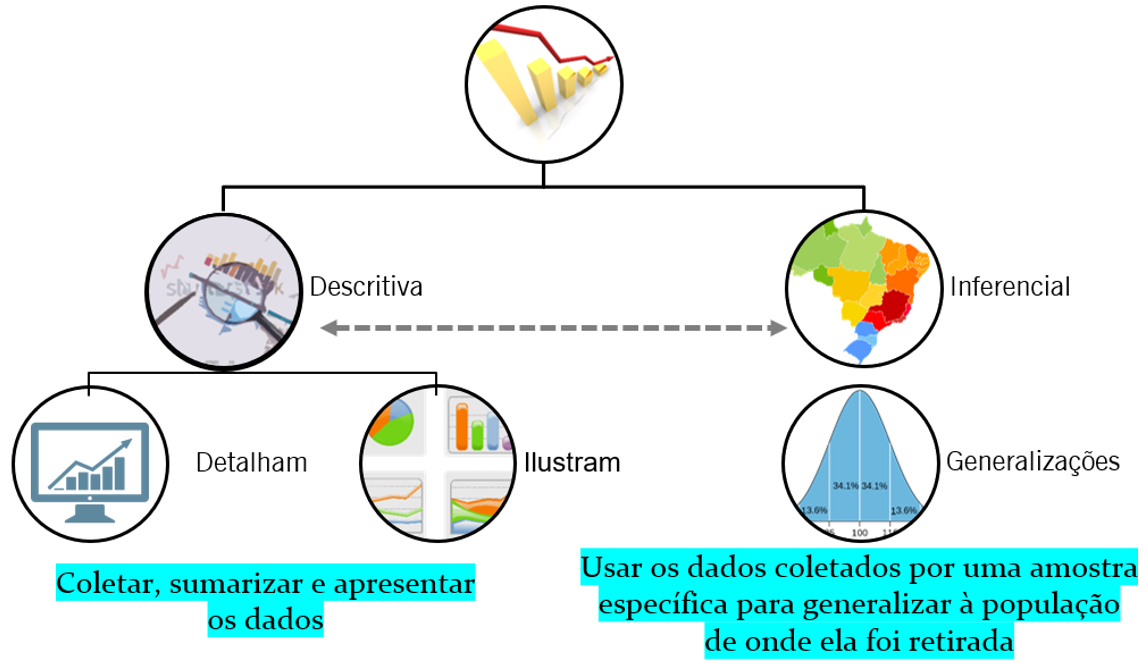
\includegraphics{./img/cap_areas_estatistica.png}

\hypertarget{resumo-1}{%
\section{Resumo}\label{resumo-1}}

\begin{enumerate}
\def\labelenumi{\arabic{enumi}.}
\tightlist
\item
  A estatística está totalmente integrada ao planejamento, execução e análise de dados de uma pesquisa\\
\item
  As pesquisas apresentam objetivos, dimensões temporais e procedimentos específicos para coleta de dados\\
\item
  Em relação ao objetivo, uma pesquisa pode ser exploratória, descritiva ou explicativa\\
\item
  Em relação à dimensão temporal, uma pesquisa pode ser transversal ou longitudinal\\
\item
  Em relação ao delineamento, uma pesquisa pode ser observacional ou experimental\\
\item
  Cientistas constroem modelos teóricos pela impossibilidade de acessar diretamente seu objeto ou fenômeno de investigação\\
\item
  As variáveis são características que podem apresentar quaisquer valores\\
\item
  A VI também é chamada de preditora, enquanto a VD é chamada de prevista\\
\item
  Em todo relacionamento bivariado, outros fatores estão envolvidos e são chamados de variáveis estranhas\\
\item
  Com muita frequência, em ciência se substitui os termos certeza e verdade por evidência e probabilidade.
\end{enumerate}

\hypertarget{questuxf5es}{%
\section{Questões}\label{questuxf5es}}

\begin{enumerate}
\def\labelenumi{\arabic{enumi}.}
\tightlist
\item
  (ENADE, 2015) O profissional de marketing de uma empresa de cosméticos foi encarregado de redesenhar o aparelho de depilação feminino comercializado por essa empresa. Para tanto, o profissional fez uma pesquisa de mercado utilizando entrevistas e discussões em grupo (grupo focal) com mulheres de segmentos diferentes do mercado-alvo potencial do produto, tendo em vista que a depilação é considerada uma experiência pessoal pelas mulheres. Esta é uma pesquisa exploratória.a) Verdadeirob) Falso
\end{enumerate}

Gabarito: 1b

\hypertarget{estatuxedstica-descritiva}{%
\chapter{Estatística Descritiva}\label{estatuxedstica-descritiva}}

\textbf{Objetivos do capítulo}\\
1. Introduzir conceitos importantes em estatística descritiva\\
2. Apresentar tabelas e gráficos\\
3. Apresentar funções do dplyr e ggplot\\
4. Apresentar um módulo específico do JASP\\
5. Sugerir heurísticas ou regras gerais na criação de gráficos

Quando pesquisadores e acadêmicos fazem seus estudos, com muita frequência, eles obtêm um grande conjunto de dados, sendo pouco informativo ou até mesmo inviável apresentar detalhadamente todos eles. A estatística descritiva oferece uma diversidade de ferramentas que auxiliam a organizar, descrever, resumir e apresentar os dados obtidos, de forma que os resultados sejam mais fáceis de serem compreendidos e analisados e, consequentemente, que a pesquisa possa ser melhor compreendida por todos os seus leitores.

\textbf{Atenção}: A estatística descritiva dispõe de inúmeras ferramentas para auxiliar na gestão e apresentação de dados.

Frequentemente, a massa de dados obtidos em uma pesquisa (realização) é resumida por alguns números específicos, que possuem certas propriedades estatísticas, e conseguem sintetizar adequadamente o volume de dados. Por sua vez, esses números são úteis em análises que possam ser necessárias e serão descritos em outra seção deste capítulo.

Na apresentação dos dados, é possível utilizar informações textuais, tabelas e gráficos. Tabelas e textos permitem agrupar e detalhar os resultados e, com isso, torná-los mais precisos e detalhados. Entretanto, esse aprofundamento pode também dificultar o entendimento geral do estudo. Por sua vez, gráficos geram sumários descritivos, em que é possível ter um entendimento rápido dos principais resultados. Eles também podem incorporar elementos adicionais, que possibilitam uma primeira análise inferencial, tal como barras de erro e intervalos de confiança. Dependendo do tipo de gráfico, além da apresentação de resultados descritivos, é possível também expor diferenças entre grupos ou relações entre variáveis.

Apesar dessas vantagens, algumas limitações podem ser encontradas nos gráficos. Uma vez que os eles condensam um grande conjunto de resultados em uma apresentação mais simples, eles podem dificultar um pouco no entendimento geral das conclusões obtidas pela pesquisa e, ocasionalmente, distorcer os resultados.

No geral, cada uma dessa formas de apresentar os resultados de uma pesquisa traz consigo vantagens e desvantagens, listadas a seguir:

\begin{longtable}[]{@{}ll@{}}
\toprule
\begin{minipage}[b]{0.47\columnwidth}\raggedright
Tabelas\strut
\end{minipage} & \begin{minipage}[b]{0.47\columnwidth}\raggedright
Gráficos\strut
\end{minipage}\tabularnewline
\midrule
\endhead
\begin{minipage}[t]{0.47\columnwidth}\raggedright
\textbf{Vantagens}\strut
\end{minipage} & \begin{minipage}[t]{0.47\columnwidth}\raggedright
\strut
\end{minipage}\tabularnewline
\begin{minipage}[t]{0.47\columnwidth}\raggedright
Auxiliam a organizar os resultados\strut
\end{minipage} & \begin{minipage}[t]{0.47\columnwidth}\raggedright
Condensam vários resultados\strut
\end{minipage}\tabularnewline
\begin{minipage}[t]{0.47\columnwidth}\raggedright
Permitem detalhar e aprofundar os resultados\strut
\end{minipage} & \begin{minipage}[t]{0.47\columnwidth}\raggedright
Auxiliam a identificar padrões nos resultados\strut
\end{minipage}\tabularnewline
\begin{minipage}[t]{0.47\columnwidth}\raggedright
Apresentam os resultados de maneira mais precisa\strut
\end{minipage} & \begin{minipage}[t]{0.47\columnwidth}\raggedright
Auxiliam a visualizar o relacionamento entre variáveis\strut
\end{minipage}\tabularnewline
\begin{minipage}[t]{0.47\columnwidth}\raggedright
Buscadores (google, etc) encontram os resultados\strut
\end{minipage} & \begin{minipage}[t]{0.47\columnwidth}\raggedright
Permitem confirmar ou não suposições incialmente feitas sobre os dados\strut
\end{minipage}\tabularnewline
\begin{minipage}[t]{0.47\columnwidth}\raggedright
\strut
\end{minipage} & \begin{minipage}[t]{0.47\columnwidth}\raggedright
Fáceis de serem entendidos quando bem feitos\strut
\end{minipage}\tabularnewline
\begin{minipage}[t]{0.47\columnwidth}\raggedright
\textbf{Limitações}\strut
\end{minipage} & \begin{minipage}[t]{0.47\columnwidth}\raggedright
\strut
\end{minipage}\tabularnewline
\begin{minipage}[t]{0.47\columnwidth}\raggedright
Podem dificultar o entendimento dos resultados\strut
\end{minipage} & \begin{minipage}[t]{0.47\columnwidth}\raggedright
Podem simplificar demasiadamente os resultados\strut
\end{minipage}\tabularnewline
\begin{minipage}[t]{0.47\columnwidth}\raggedright
\strut
\end{minipage} & \begin{minipage}[t]{0.47\columnwidth}\raggedright
Podem distorcer severamente os resultados quando mal feitos\strut
\end{minipage}\tabularnewline
\bottomrule
\end{longtable}

É importante atentar que em todas estas técnicas, mas especialmente nas gráficas, deve-se evitar gerar distorções ao entendimento e interpretação dos resultados. Há casos de pessoas e profissionais que chegaram a sofrer sanções jurídicas por distorções intencionais em apresentação estatísticas. Há recomendações nacionais e internacionais que visam auxiliar no desenvolvimento de gráficos e tabelas e, com grande frequência, periódicos e editoras também exigem formatos específicos na apresentação dos resultados.

\hypertarget{tabelas}{%
\section{Tabelas}\label{tabelas}}

As tabelas são recursos estatísticos que permitem a apresentação dos resultados de uma pesquisa de maneira resumida, reunida e objetiva. É possível utilizá-las para apresentação de apenas uma ou múltiplas variáveis, que podem ser categóricas ou contínuas. Todas as tabelas precisam de títulos e, eventualmente, algumas notas podem auxiliar no entendimento dos resultados.

O formato padronizado para desenvolvimento de tabelas costuma variar de revista para revista No entanto, é possível notar que, quase sempre, os números são arredondados em 2 casas decimais e apenas as linhas possuem bordas. A imagem abaixo apresenta uma tabela construída pelas recomendações da American Psychological Association (APA).

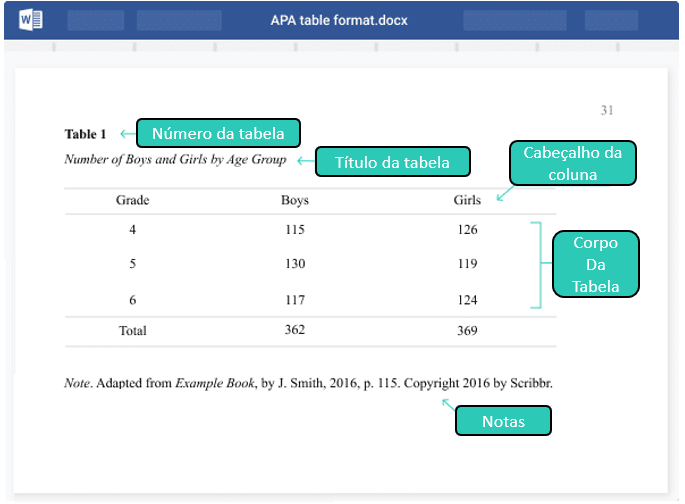
\includegraphics{./img/cap_desc_tabela.png}

\hypertarget{gruxe1ficos}{%
\section{Gráficos}\label{gruxe1ficos}}

Gráficos são representações visuais utilizadas para exibir dados. Da mesma forma que tabelas, eles podem ser formados por uma ou múltiplas variáveis. Quando uma única variável é apresentada em um gráfico, sua finalidade tende a ser apenas descritiva. Quando duas ou mais variáveis são apresentadas, eles auxiliam a comparar os resultados entre grupos ou explorar o relacionamento entre variáveis.

Se bem feitos, os gráficos são extremamente úteis e auxiliam o rápido entendimento dos resultados obtidos em uma pesquisa. Como aponta Morettin e Bussab \earpar{morettin_bussab_2010}, eles possibilitam:

\begin{enumerate}
\def\labelenumi{(\alph{enumi})}
\tightlist
\item
  Buscar padrões e relações;\\
\item
  Confirmar (ou não) certas expectativas que se tinha sobre os dados;\\
\item
  Descobrir novos fenômenos;\\
\item
  Confirmar (ou não) suposições feitas sobre os procedimentos estatísticos usados; e\\
\item
  Apresentar resultados de modo mais rápido e fácil.
\end{enumerate}

É sempre importante que o gráfico tenha um título e uma escala e, quando necessário, notas complementares.

A maioria dos gráficos são construídos em um plano com um eixo horizontal (abscissas) e um vertical (ordenadas). Quando há apenas uma variável para apresentar, o eixo X irá reunir os níveis ou possíveis valores desta variável, enquanto o eixo Y irá apresentar suas contagens, proporções ou densidade. Quando há duas variáveis, o eixo X será utilizado para apresentar os níveis ou possíveis valores da variável independente, enquanto o Y apresentará os valores médios encontrados na variável dependente, tal como apresentado a seguir.

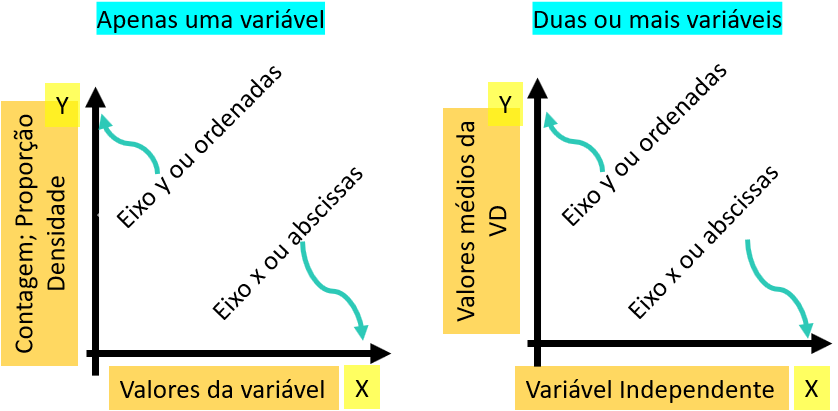
\includegraphics{./img/cap_grafico_tutorial.png}

Quando há mais de uma variável independente, um agrupador ou cluster deverá ser apresentado. Com frequência, o eixo X recebe a variável independente com mais níveis, enquanto o agrupador recebe as outras. A imagem a seguir descreve este cenário.

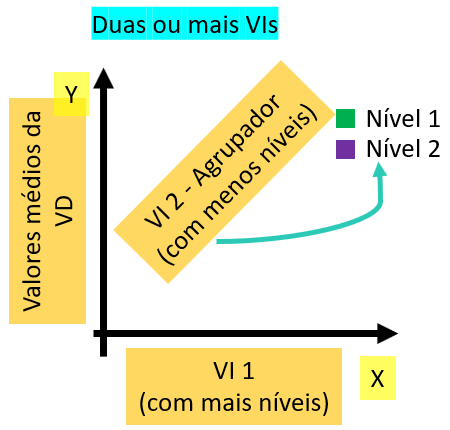
\includegraphics{./img/cap_grafico_tutorial2.png}

Há diferentes heurísticas que auxiliam na escolha de um gráfico adequado para apresentar os resultados de uma pesquisa. De forma geral, essa escolha pode ser pautada por duas perguntas:

\begin{enumerate}
\def\labelenumi{\arabic{enumi}.}
\tightlist
\item
  Quantas variáveis serão apresentadas ?\\
\item
  Qual o nível de medida da variável (ou variável independente quando há duas ou mais)?
\end{enumerate}

Com isso, o diagrama abaixo oferece uma árvore de decisão funcional.

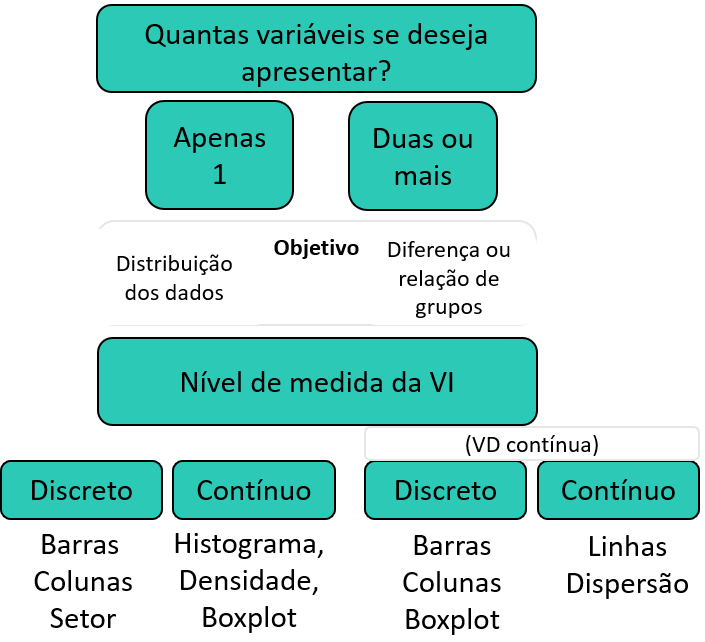
\includegraphics{./img/cap_como_fazer_graficos.png}

\emph{Nota: Nessa apresentação, pragmaticamente as variáveis categóricas são tratadas como discretas.}

A imagem a seguir ilustra alguns desses gráficos. Suas características serão apresentadas em seguida.

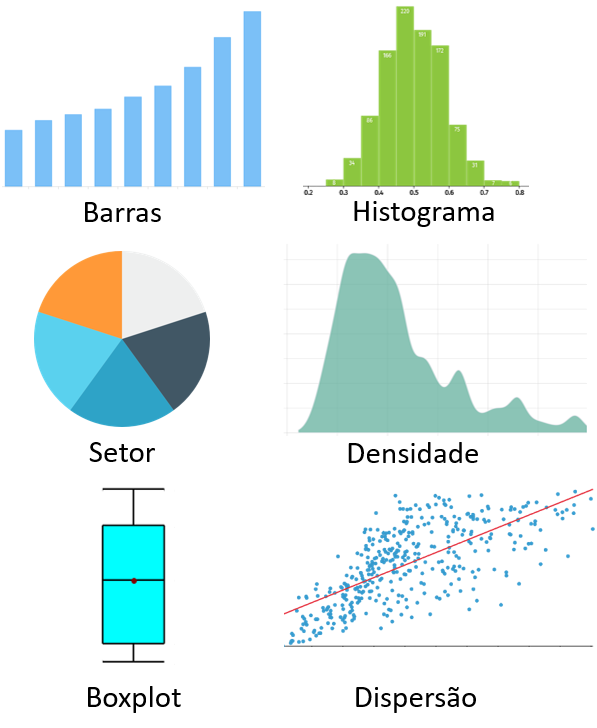
\includegraphics{./img/cap_graficos.png}

A apresentação de gráficos tende a seguir um desenvolvimento hierárquico. Inicialmente, gráficos univariados para variáveis categóricas e contínuas são criados. Em seguida, gráficos apresentando diferenças e relações entre grupos e variáveis são feitos. Na seção \protect\hyperlink{pesquisa}{Pesquisa}, diferentes gráficos serão gerados para ilustrar o processo.

\hypertarget{medidas-de-posiuxe7uxe3o-e-dispersuxe3o}{%
\section{Medidas de posição e dispersão}\label{medidas-de-posiuxe7uxe3o-e-dispersuxe3o}}

Uma vez que é pragmaticamente inviável apresentar detalhadamente todos os dados obtidos em uma pesquisa, há um conjunto de números podem ser utilizados para resumir todo o conjunto. Eles costumam ser chamados de números-síntese, medidas resumo, medidas estatísticas ou apenas estatísticas e podem ser agrupados em medidas de posição e medidas de dispersão, que serão descritas a seguir.

Medidas de posição: São valores que representam a concentração dos dados observados. Podem ser divididas em medidas de tendência central, medidas separatrizes e medidas de posição relativa.

As medidas de tendência central (MTC) indicam o valor em torno do qual uma grande proporção de outros valores está centralizada. As MTC mais usadas são a moda, a média e a mediana.

As separatrizes também são chamadas de quantis ou medidas de ordenamento. Elas são valores que indicam posições em uma distribuição ordenada acumulada dos dados. Os principais quantis utilizados são os quartis (divisão dos dados em 4 partes iguais), decis (divisão em 10 partes iguais) e percentis (divisão em 100 partes iguais).

As medidas de posição relativa são as vezes chamadas de Escore padrão. Elas são valores que indicam as posições que cada valor do conjunto de dados em relação a todos os dados. O Escore Z, o Escore T e o Escore QI tendem a ser classificados como como medidas de posição de relativa e são bastante utilizados em Psicometria.

É possível notar que essa divisão tão detalhada pode gerar inconsistências e é raramente utilizada na prática. No dia a dia, as medidas de tendência central abrangem pragmaticamente todas as medidas de posição.

Medidas de dispersão : Também chamadas de medidas de variabilidade ou afastamento. São valores que indicam o quão dispersa se encontra a distribuição dos valores em relação à alguma medida de tendência central. Entre as medidas de dispersão, estão a amplitude, a amplitude (ou intervalo) interquartil, a variância, o desvio-padrão e o coeficiente de variação. Em Psicologia, o desvio-padrão e a amplitude interquartil (também chamado de intervalo interquartil) são as mais utilizadas.

O diagrama abaixo apresenta estas informações.

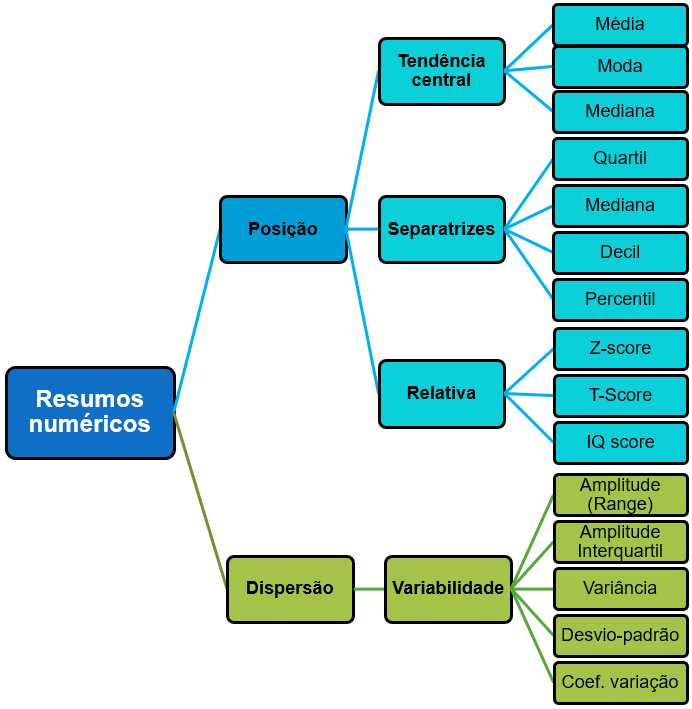
\includegraphics{./img/cap_desc_medidas_posicao_dispersao.png}

Como previamente comentado, esse detalhamento tem pouco sentido prático na maioria das pesquisas. Apenas em raras exceções, como em Psicometria, é que discussões sobre percentis e Escores Z são feitas. Assim, apesar do esforço feito para reunir as principais medidas estatísticas utilizadas, a organização apresentada no diagrama a seguir traz maior utilidade.

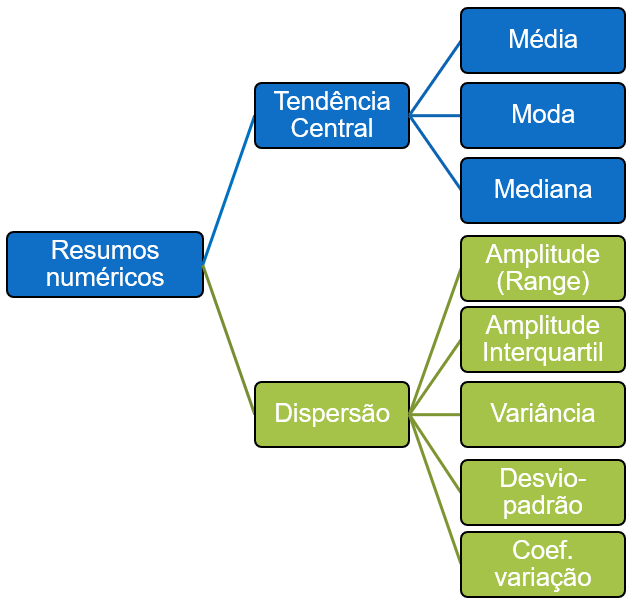
\includegraphics{./img/cap_desc_medidas_posicao_dispersao2.png}

As principais medidas serão agora apresentadas de uma maneira simples. Esse formato é proposital, uma vez que a proposta do livro é discutir tais conceitos pela apresentação de pesquisas específicas e previamente publicadas.

\hypertarget{muxe9dia}{%
\section{Média}\label{muxe9dia}}

A média é a MTC mais comum e mais intuitiva. Seu valor representa o ``centro de gravidade'' da distribuição, descrevendo a maior concentração dos valores em torno dela. Assim, ela resume o conjunto de dados e pode ser utilizada para substituir os outros valores, o que é especialmente útil quando há casos ausentes.

Para ilustrar, imagine a seguinte situação: 10 pacientes foram avaliados por um teste de inteligência e apresentaram os resultados abaixo descritos:

\emph{90.6}, \emph{102.8}, \emph{87.47}, \emph{123.9}, \emph{104.9}, \emph{87.69}, \emph{107.3}, \emph{111.1}, \emph{108.6}, \emph{95.42} and \emph{122.7}

A média indicará o valor central da distribuição em relação à distância entre os outros valores.

\emph{103.9}

Caso uma tabela seja apresentada e nela seja calculada a distância de todos os valores em relação à média, os resultados seriam assim:

\begin{longtable}[]{@{}ccc@{}}
\toprule
\begin{minipage}[b]{0.15\columnwidth}\centering
Resultado\strut
\end{minipage} & \begin{minipage}[b]{0.10\columnwidth}\centering
media\strut
\end{minipage} & \begin{minipage}[b]{0.15\columnwidth}\centering
distancia\strut
\end{minipage}\tabularnewline
\midrule
\endhead
\begin{minipage}[t]{0.15\columnwidth}\centering
90.6\strut
\end{minipage} & \begin{minipage}[t]{0.10\columnwidth}\centering
103.9\strut
\end{minipage} & \begin{minipage}[t]{0.15\columnwidth}\centering
-13.26\strut
\end{minipage}\tabularnewline
\begin{minipage}[t]{0.15\columnwidth}\centering
102.8\strut
\end{minipage} & \begin{minipage}[t]{0.10\columnwidth}\centering
103.9\strut
\end{minipage} & \begin{minipage}[t]{0.15\columnwidth}\centering
-1.11\strut
\end{minipage}\tabularnewline
\begin{minipage}[t]{0.15\columnwidth}\centering
87.47\strut
\end{minipage} & \begin{minipage}[t]{0.10\columnwidth}\centering
103.9\strut
\end{minipage} & \begin{minipage}[t]{0.15\columnwidth}\centering
-16.4\strut
\end{minipage}\tabularnewline
\begin{minipage}[t]{0.15\columnwidth}\centering
123.9\strut
\end{minipage} & \begin{minipage}[t]{0.10\columnwidth}\centering
103.9\strut
\end{minipage} & \begin{minipage}[t]{0.15\columnwidth}\centering
20.06\strut
\end{minipage}\tabularnewline
\begin{minipage}[t]{0.15\columnwidth}\centering
104.9\strut
\end{minipage} & \begin{minipage}[t]{0.10\columnwidth}\centering
103.9\strut
\end{minipage} & \begin{minipage}[t]{0.15\columnwidth}\centering
1.078\strut
\end{minipage}\tabularnewline
\begin{minipage}[t]{0.15\columnwidth}\centering
87.69\strut
\end{minipage} & \begin{minipage}[t]{0.10\columnwidth}\centering
103.9\strut
\end{minipage} & \begin{minipage}[t]{0.15\columnwidth}\centering
-16.17\strut
\end{minipage}\tabularnewline
\begin{minipage}[t]{0.15\columnwidth}\centering
107.3\strut
\end{minipage} & \begin{minipage}[t]{0.10\columnwidth}\centering
103.9\strut
\end{minipage} & \begin{minipage}[t]{0.15\columnwidth}\centering
3.447\strut
\end{minipage}\tabularnewline
\begin{minipage}[t]{0.15\columnwidth}\centering
111.1\strut
\end{minipage} & \begin{minipage}[t]{0.10\columnwidth}\centering
103.9\strut
\end{minipage} & \begin{minipage}[t]{0.15\columnwidth}\centering
7.211\strut
\end{minipage}\tabularnewline
\begin{minipage}[t]{0.15\columnwidth}\centering
108.6\strut
\end{minipage} & \begin{minipage}[t]{0.10\columnwidth}\centering
103.9\strut
\end{minipage} & \begin{minipage}[t]{0.15\columnwidth}\centering
4.772\strut
\end{minipage}\tabularnewline
\begin{minipage}[t]{0.15\columnwidth}\centering
95.42\strut
\end{minipage} & \begin{minipage}[t]{0.10\columnwidth}\centering
103.9\strut
\end{minipage} & \begin{minipage}[t]{0.15\columnwidth}\centering
-8.445\strut
\end{minipage}\tabularnewline
\begin{minipage}[t]{0.15\columnwidth}\centering
122.7\strut
\end{minipage} & \begin{minipage}[t]{0.10\columnwidth}\centering
103.9\strut
\end{minipage} & \begin{minipage}[t]{0.15\columnwidth}\centering
18.81\strut
\end{minipage}\tabularnewline
\bottomrule
\end{longtable}

Somando as distâncias, o resultado será \texttt{0}, indicando que elas se anulam e que a média é o centro da distribuição.

\begin{longtable}[]{@{}ccc@{}}
\toprule
\begin{minipage}[b]{0.15\columnwidth}\centering
Resultado\strut
\end{minipage} & \begin{minipage}[b]{0.10\columnwidth}\centering
media\strut
\end{minipage} & \begin{minipage}[b]{0.15\columnwidth}\centering
distancia\strut
\end{minipage}\tabularnewline
\midrule
\endhead
\begin{minipage}[t]{0.15\columnwidth}\centering
90.6\strut
\end{minipage} & \begin{minipage}[t]{0.10\columnwidth}\centering
103.9\strut
\end{minipage} & \begin{minipage}[t]{0.15\columnwidth}\centering
-13.3\strut
\end{minipage}\tabularnewline
\begin{minipage}[t]{0.15\columnwidth}\centering
102.8\strut
\end{minipage} & \begin{minipage}[t]{0.10\columnwidth}\centering
103.9\strut
\end{minipage} & \begin{minipage}[t]{0.15\columnwidth}\centering
-1.1\strut
\end{minipage}\tabularnewline
\begin{minipage}[t]{0.15\columnwidth}\centering
87.5\strut
\end{minipage} & \begin{minipage}[t]{0.10\columnwidth}\centering
103.9\strut
\end{minipage} & \begin{minipage}[t]{0.15\columnwidth}\centering
-16.4\strut
\end{minipage}\tabularnewline
\begin{minipage}[t]{0.15\columnwidth}\centering
123.9\strut
\end{minipage} & \begin{minipage}[t]{0.10\columnwidth}\centering
103.9\strut
\end{minipage} & \begin{minipage}[t]{0.15\columnwidth}\centering
20.1\strut
\end{minipage}\tabularnewline
\begin{minipage}[t]{0.15\columnwidth}\centering
104.9\strut
\end{minipage} & \begin{minipage}[t]{0.10\columnwidth}\centering
103.9\strut
\end{minipage} & \begin{minipage}[t]{0.15\columnwidth}\centering
1.1\strut
\end{minipage}\tabularnewline
\begin{minipage}[t]{0.15\columnwidth}\centering
87.7\strut
\end{minipage} & \begin{minipage}[t]{0.10\columnwidth}\centering
103.9\strut
\end{minipage} & \begin{minipage}[t]{0.15\columnwidth}\centering
-16.2\strut
\end{minipage}\tabularnewline
\begin{minipage}[t]{0.15\columnwidth}\centering
107.3\strut
\end{minipage} & \begin{minipage}[t]{0.10\columnwidth}\centering
103.9\strut
\end{minipage} & \begin{minipage}[t]{0.15\columnwidth}\centering
3.4\strut
\end{minipage}\tabularnewline
\begin{minipage}[t]{0.15\columnwidth}\centering
111.1\strut
\end{minipage} & \begin{minipage}[t]{0.10\columnwidth}\centering
103.9\strut
\end{minipage} & \begin{minipage}[t]{0.15\columnwidth}\centering
7.2\strut
\end{minipage}\tabularnewline
\begin{minipage}[t]{0.15\columnwidth}\centering
108.6\strut
\end{minipage} & \begin{minipage}[t]{0.10\columnwidth}\centering
103.9\strut
\end{minipage} & \begin{minipage}[t]{0.15\columnwidth}\centering
4.8\strut
\end{minipage}\tabularnewline
\begin{minipage}[t]{0.15\columnwidth}\centering
95.4\strut
\end{minipage} & \begin{minipage}[t]{0.10\columnwidth}\centering
103.9\strut
\end{minipage} & \begin{minipage}[t]{0.15\columnwidth}\centering
-8.4\strut
\end{minipage}\tabularnewline
\begin{minipage}[t]{0.15\columnwidth}\centering
122.7\strut
\end{minipage} & \begin{minipage}[t]{0.10\columnwidth}\centering
103.9\strut
\end{minipage} & \begin{minipage}[t]{0.15\columnwidth}\centering
18.8\strut
\end{minipage}\tabularnewline
\begin{minipage}[t]{0.15\columnwidth}\centering
Total\strut
\end{minipage} & \begin{minipage}[t]{0.10\columnwidth}\centering
-\strut
\end{minipage} & \begin{minipage}[t]{0.15\columnwidth}\centering
3.109e-15\strut
\end{minipage}\tabularnewline
\bottomrule
\end{longtable}

A tabela a seguir apresenta algumas características vantajosas e possíveis limitações da média.

\begin{longtable}[]{@{}ll@{}}
\toprule
Vantagem & Limitação\tabularnewline
\midrule
\endhead
É intuitiva & Sensível\tabularnewline
Algebricamente tratável & Não adequada a dados nominais\tabularnewline
Estimador não viesado &\tabularnewline
Sensível &\tabularnewline
\bottomrule
\end{longtable}

\emph{Nota: Uma medida sensível significa que ela é influenciada por todos os outros valores.}

Exemplo de aplicações: Praticamente, em todas as pesquisas se utiliza a média para resumir o volume de dados obtidos. Como exemplos em Psicologia, a média de valores de inventários e testes psicológicos, a média do tempo de reação que um participante demora para responder à uma atividade específica e a média de consultas clínicas que em média um profissional realiza.

\hypertarget{mediana}{%
\section{Mediana}\label{mediana}}

A mediana é uma medida que representa o centro do conjunto de dados quando se considera a quantidade de elementos presentes. Portanto, a mediana divide a quantidade de dados em duas partes iguais, em que 50\% dos dados estão abaixo dela e 50\% dos dados estão acima dela. A mediana pode ser classificada tanto como uma medida de tendência central, como uma separatriz \citep{neto2010}.

Dessa forma, os resultados da mediana são iguais aos resultados do 2º quartil, 5º decil e percentil 50. Comparada com a média, os resultados obtido pela mediana são mais robustos ou resistentes aos valores atípicos ou anômalos, apesar de menos intuitivos.

Para dividir a distribuição em duas partes iguais, a realização da mediana precisa de alguns procedimentos. Repare que abaixo estão os mesmos resultados apresentados na seção da média:

\emph{90.6}, \emph{102.8}, \emph{87.47}, \emph{123.9}, \emph{104.9}, \emph{87.69}, \emph{107.3}, \emph{111.1}, \emph{108.6}, \emph{95.42} and \emph{122.7}

Para o cálculo da mediana, é necessário organizar essa série de valores de maneira ascendente (chamado de rol) e localizar o resultado ao centro. Nesse caso, o valor ao centro é \texttt{104.9} . Note que este valor divide os dados em duas partes iguais de elementos abaixo ou acima dele.

\emph{87.47}, \emph{87.69}, \emph{90.6}, \emph{95.42}, \emph{102.8}, \emph{104.9}, \emph{107.3}, \emph{108.6}, \emph{111.1}, \emph{122.7} and \emph{123.9}

Caso a quantidade de elementos seja ímpar, a localização da mediana é mais fácil. Caso esta quantidade seja par, a mediana será calculada pela média aritmética dos dois elementos centrais.

A tabela a seguir descreve algumas características vantajosas e possíveis limitações da mediana.

\begin{longtable}[]{@{}ll@{}}
\toprule
\begin{minipage}[b]{0.47\columnwidth}\raggedright
Vantagem\strut
\end{minipage} & \begin{minipage}[b]{0.47\columnwidth}\raggedright
Limitação\strut
\end{minipage}\tabularnewline
\midrule
\endhead
\begin{minipage}[t]{0.47\columnwidth}\raggedright
Resistente a valor anômalos/Outliers\strut
\end{minipage} & \begin{minipage}[t]{0.47\columnwidth}\raggedright
Não representa todos os valores\strut
\end{minipage}\tabularnewline
\begin{minipage}[t]{0.47\columnwidth}\raggedright
Adequada para dados ordinais, intervalares e de razão\strut
\end{minipage} & \begin{minipage}[t]{0.47\columnwidth}\raggedright
Não adequada a dados nominais\strut
\end{minipage}\tabularnewline
\begin{minipage}[t]{0.47\columnwidth}\raggedright
\strut
\end{minipage} & \begin{minipage}[t]{0.47\columnwidth}\raggedright
Pouco adequada a tratamentos algébricos futuros\strut
\end{minipage}\tabularnewline
\bottomrule
\end{longtable}

Exemplo de aplicações: Situações em que a distribuição é muito assimétrica. Variáveis econômicas como salário e pobreza costumam trabalhar com a mediana dos dados.

\hypertarget{moda}{%
\section{Moda}\label{moda}}

A moda é a realização mais frequente de um conjunto de dados. Salvo algumas exceções, a moda não costuma ser utilizada em análises estatísticas, uma vez que representa mal o conjunto de dados.

Exemplo de aplicações: Situações em saúde pública, como a idade mais típica que uma menina tem o primeiro filho, dia e/ou horário modal de admissão em um hospital. Situações econômicas de determinação de salários mínimos, eventualmente, também pode contar com resultados modais.

\hypertarget{amplitude}{%
\section{Amplitude}\label{amplitude}}

A amplitude é uma medida de dispersão que indica a variabilidade dos dados. O procedimento para seu cálculo é a subtração entre o maior e o menor valor de um conjunto de dados.

\hypertarget{amplitude-interquartil}{%
\section{Amplitude interquartil}\label{amplitude-interquartil}}

A amplitude interquartil também é chamada de intervalo interquartil. Essa medida apresenta a variabilidade dos dados de maneira insensível a valores extremos. Ela é computada pela subtração do primeiro quartil (Q1) pelo terceiro quartil (Q3), ou seja, \texttt{Q3-Q1}. Os quartis são medidas que indicam posições de separação no conjunto ordenado de dados.

O primeiro quartil indica o valor onde estão até 25\% dos dados, o segundo quartil tem o mesmo valor da mediana e o terceiro quartil indica o valor onde estão até 75\% dos dados.

Como a amplitude interquartil considera apenas a variabilidade em torno do centro, ela é uma medida considerada mais estável ou robusta quando comparada a outras medidas de dispersão.

\hypertarget{variuxe2ncia-e-desvio-padruxe3o}{%
\section{Variância e Desvio-padrão}\label{variuxe2ncia-e-desvio-padruxe3o}}

A variância e o desvio-padrão são duas medidas de dispersão frequentemente utilizadas em estatística de maneira intercambiável.

A variância indica a variabilidade quadrática de um conjunto de dados, considerando todos os valores da distribuição. Pela sua estrutura matemática, seu resultado expressa o desvio quadrático médio e, com isso, seu valor não está na mesma unidade dos dados originais.

A variância é uma medida fundamental no estudo das famílias de distribuições de probabilidades e análises estatísticas. No entanto, na prática, ela é pouco usada para descrever a variabilidade dos dados e acaba sendo usada apenas de forma transitória para o cálculo do desvio-padrão.

O desvio-padrão indica a variação dos valores em torno da média, e como seus resultados são calculados pela raiz quadrada da variância, o desvio-padrão está na mesma unidade dos dados originais. Dessa forma, o desvio-padrão tem uma melhor característica descritiva.

Em síntese, enquanto a variância possui maior importância em aspectos matemáticos relacionados às famílias de distribuições de probabilidade, o desvio-padrão tem melhor adequação descritiva de um conjunto de dados. Conceitualmente, as equações a seguir descrevem à variância amostral (à esquerda) e o desvio-padrão amostral (à direita):

\begin{equation}
  \begin{split}
    S^2 = \sqrt\frac{\sum\limits_{i=1}^N (X -\mu)^2}{N-1}
  \end{split}
\qquad\qquad
  \begin{split}
    S = \frac{\sum\limits_{i=1}^N (X -\mu)^2}{N-1}
  \end{split}
\end{equation}

Após estas apresentações teóricas, espera-se que seja possível apresentar a pesquisa a seguir, bem como implementar parte dos conceitos nos dados obtidos.

\hypertarget{momentos-estatuxedsticos}{%
\section{Momentos estatísticos}\label{momentos-estatuxedsticos}}

O conceito de momentos em estatística é bastante útil para destacar um conjunto de fórmulas que permitem descrever o conjunto de dados obtidos em uma pesquisa \citep{JenkinsSmith2017}. Tecnicamente, ele resume o que foi apresentado separadamente nas medidas de posição e dispersão. Por eles serem descritos em formato analítico, acabam sendo pouco comentados em Psicologia, infelizmente.

\begin{enumerate}
\def\labelenumi{\arabic{enumi}.}
\tightlist
\item
  A média (valor esperado) \(E[X]\):
\end{enumerate}

\[E(X) = \bar{X}=\frac{\sum X_{i}}{n}\]

\begin{enumerate}
\def\labelenumi{\arabic{enumi}.}
\setcounter{enumi}{1}
\tightlist
\item
  Variância amostral (\(S^2\)):
\end{enumerate}

\[s^{2}_{x}=\frac{\sum (X-\bar{X})^{2}}{(n-1)}\]

\begin{enumerate}
\def\labelenumi{\arabic{enumi}.}
\setcounter{enumi}{2}
\tightlist
\item
  Assimetria (\(AS\)):
\end{enumerate}

\[AS = \frac{\sum (X-\bar{X})^{3}}{(n-1)}/\sigma^3 = \frac{1}{n-1} *\frac{\sum (X-\bar{X})^3}{\sigma^3}\]

Caso o Coeficiente de Assimetria seja igual a 0, não há assimetria.

\begin{enumerate}
\def\labelenumi{\arabic{enumi}.}
\setcounter{enumi}{3}
\tightlist
\item
  Curtose (\(K\)):\\
  \[K = \frac{\sum (X-\bar{X})^{4}}{(n-1)}/\sigma^4= \frac{1}{n-1} *\frac{\sum (X-\bar{X})^4}{({\sigma^2})^2}\]
\end{enumerate}

Indica o achatamento. Caso o Coeficiente de Kurtose seja igual a 3, o formato da distribuição é simétrico ou Mesocúrtica. Caso seja menor do que 3, ela tem formato platicurtico (baixa com caudas curtas) e acima de 3 o formato é leptocurtico (alta com caudas longas).

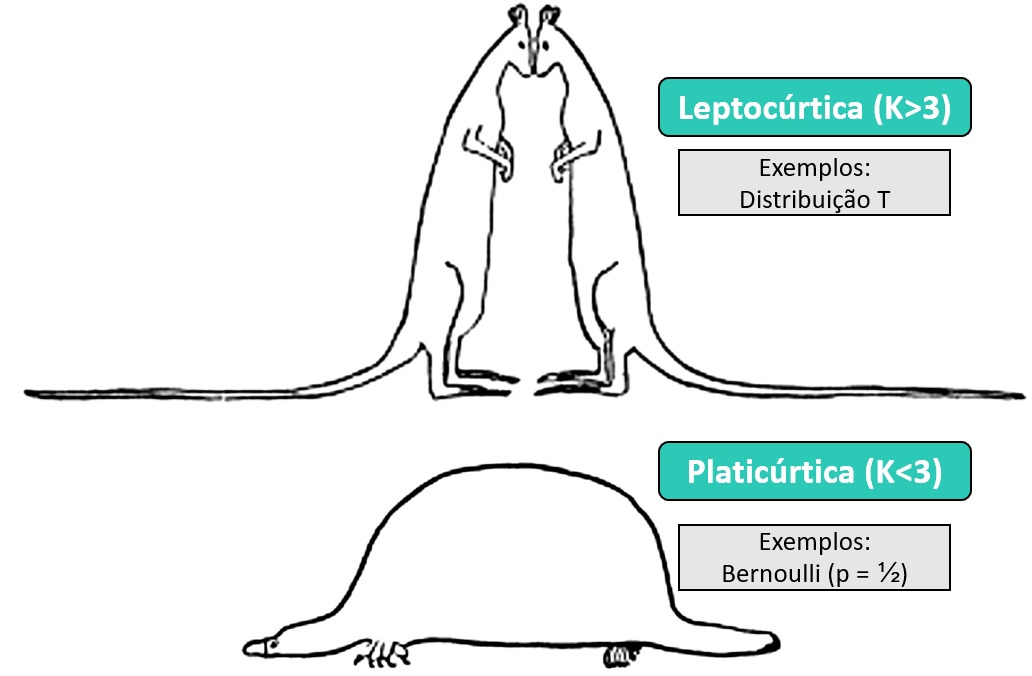
\includegraphics{./img/cap_desc_curtose.png}

Coletaral a apresentação, o surgimento do termo ``momentos estatísticos'' parece ter surgido de trabalhos de Pearson em física, especialmente sobre elasticidade, inércia e momentos de ruptura \citep{David1998}

\hypertarget{pesquisa}{%
\section{Pesquisa}\label{pesquisa}}

A base desta pesquisa está disponível em formato \textbf{R (Rdata)} e em \textbf{CSV}, que é lido pelo JASP. Clique na opção desejada.

Base R: \href{https://github.com/anovabr/mqt/raw/master/bases/Base\%20R\%20-\%20Pesquisa\%20mapfre.RData}{Base R - Pesquisa mapfre.RData}\\
Base JASP: \href{https://github.com/anovabr/mqt/raw/master/bases/bases_csv_jasp.zip}{Base CSV - dataset\_mapfre}

Neste capítulo, vamos utilizar a pesquisa intitulada \href{https://doi.org/10.1590/0102.3772e36412}{``Depression and Anxiety Symptoms in a Representative Sample of Undergraduate Students in Spain, Portugal, and Brazil''}. Nessa pesquisa, sou o coautor e o pesquisador responsável para correspondência. O objetivo deste estudo foi desenvolver um mapa epidemiológico de sintomas de ansiedade e depressão em universitários em três países, bem como investigar possíveis relações entre tais condições de saúde e fatores sociodemográficos. Para acessar eventuais transtornos depressivos, o Inventário Beck de Depressão (BDI) foi utilizado e para acessar condições de ansiedade, o Inventário Beck de Ansiedade (BAI) foi utilizado. Em ambos os inventários, valores altos sugerem que condições de agravo à saúde mental podem estar presentes.

Um diferencial importante do trabalho foi a seleção amostral. Partiu-se de uma amostra estratificada (probabilística) dos estudantes de três universidades, PUC-Rio (Brasil), Universidade de Extremadura (Espanha) e Universidade de Coimbra (Portugal). Isso permitiu ter maior validade externa dos resultados.

\hypertarget{execuuxe7uxe3o-no-r}{%
\section{Execução no R}\label{execuuxe7uxe3o-no-r}}

Inicialmente, é necessário carregar a base de dados previamente descrita para o ambiente R. Este procedimento será necessário para todos os capítulos do livro.

Frequentemente, uma primeira tabela informativa começa descrevendo as variáveis categóricas, que deve apresentar suas contagens e proporções. Nesta pesquisa de agora, tanto a variável country como sex são categóricas e serão utilizadas.

como três países fizeram parte da pesquisa, os dados serão agrupados por eles. O desenvolvimento desta tabela pode ser feito com pacote \texttt{janitor}, tal como demonstrado a seguir.

\begin{Shaded}
\begin{Highlighting}[]
\NormalTok{Dataset }\OperatorTok\StringTok{ }
\StringTok{  }\KeywordTok{tabyl}\NormalTok{(country) }\OperatorTok\StringTok{ }
\StringTok{  }\KeywordTok{adorn_totals}\NormalTok{() }\OperatorTok\StringTok{ }
\StringTok{  }\KeywordTok{pander}\NormalTok{()}
\end{Highlighting}
\end{Shaded}

\begin{longtable}[]{@{}ccc@{}}
\toprule
\begin{minipage}[b]{0.14\columnwidth}\centering
country\strut
\end{minipage} & \begin{minipage}[b]{0.09\columnwidth}\centering
n\strut
\end{minipage} & \begin{minipage}[b]{0.13\columnwidth}\centering
percent\strut
\end{minipage}\tabularnewline
\midrule
\endhead
\begin{minipage}[t]{0.14\columnwidth}\centering
SPAIN\strut
\end{minipage} & \begin{minipage}[t]{0.09\columnwidth}\centering
1216\strut
\end{minipage} & \begin{minipage}[t]{0.13\columnwidth}\centering
0.6214\strut
\end{minipage}\tabularnewline
\begin{minipage}[t]{0.14\columnwidth}\centering
PORTUGAL\strut
\end{minipage} & \begin{minipage}[t]{0.09\columnwidth}\centering
426\strut
\end{minipage} & \begin{minipage}[t]{0.13\columnwidth}\centering
0.2177\strut
\end{minipage}\tabularnewline
\begin{minipage}[t]{0.14\columnwidth}\centering
BRAZIL\strut
\end{minipage} & \begin{minipage}[t]{0.09\columnwidth}\centering
315\strut
\end{minipage} & \begin{minipage}[t]{0.13\columnwidth}\centering
0.161\strut
\end{minipage}\tabularnewline
\begin{minipage}[t]{0.14\columnwidth}\centering
Total\strut
\end{minipage} & \begin{minipage}[t]{0.09\columnwidth}\centering
1957\strut
\end{minipage} & \begin{minipage}[t]{0.13\columnwidth}\centering
1\strut
\end{minipage}\tabularnewline
\bottomrule
\end{longtable}

A adição de um outro agrupador relacionado ao sexo é também importante. Note que existem casos ausentes nesta variável. Isso ocorre com bastante frequência e há diferentes estratégias para lidar com isso, que serão discutidas em momento oportuno. Para que valores ausentes não sejam apresentados, a função \texttt{filter} será implementada. É importante atentar que os dados ausentes não foram excluídos. Eles apenas não são apresentados.

\begin{Shaded}
\begin{Highlighting}[]
\NormalTok{Dataset }\OperatorTok\StringTok{ }
\StringTok{  }\KeywordTok{filter}\NormalTok{(}\OperatorTok{!}\KeywordTok{is.na}\NormalTok{(sex)) }\OperatorTok\StringTok{ }
\StringTok{  }\KeywordTok{tabyl}\NormalTok{(sex, country) }\OperatorTok\StringTok{ }
\StringTok{  }\KeywordTok{adorn_totals}\NormalTok{() }\OperatorTok\StringTok{ }
\StringTok{  }\KeywordTok{pander}\NormalTok{()}
\end{Highlighting}
\end{Shaded}

\begin{longtable}[]{@{}cccc@{}}
\toprule
\begin{minipage}[b]{0.10\columnwidth}\centering
sex\strut
\end{minipage} & \begin{minipage}[b]{0.10\columnwidth}\centering
SPAIN\strut
\end{minipage} & \begin{minipage}[b]{0.14\columnwidth}\centering
PORTUGAL\strut
\end{minipage} & \begin{minipage}[b]{0.14\columnwidth}\centering
BRAZIL\strut
\end{minipage}\tabularnewline
\midrule
\endhead
\begin{minipage}[t]{0.10\columnwidth}\centering
M\strut
\end{minipage} & \begin{minipage}[t]{0.10\columnwidth}\centering
384\strut
\end{minipage} & \begin{minipage}[t]{0.14\columnwidth}\centering
203\strut
\end{minipage} & \begin{minipage}[t]{0.14\columnwidth}\centering
149\strut
\end{minipage}\tabularnewline
\begin{minipage}[t]{0.10\columnwidth}\centering
F\strut
\end{minipage} & \begin{minipage}[t]{0.10\columnwidth}\centering
825\strut
\end{minipage} & \begin{minipage}[t]{0.14\columnwidth}\centering
223\strut
\end{minipage} & \begin{minipage}[t]{0.14\columnwidth}\centering
166\strut
\end{minipage}\tabularnewline
\begin{minipage}[t]{0.10\columnwidth}\centering
Total\strut
\end{minipage} & \begin{minipage}[t]{0.10\columnwidth}\centering
1209\strut
\end{minipage} & \begin{minipage}[t]{0.14\columnwidth}\centering
426\strut
\end{minipage} & \begin{minipage}[t]{0.14\columnwidth}\centering
315\strut
\end{minipage}\tabularnewline
\bottomrule
\end{longtable}

Para apresentar a quantidade total de participantes, bem como a quantidade e a porcentagem de homens e mulheres por país, a codificação torna-se um pouco mais densa. A tabela a seguir reproduz parcialmente a tabela 1 do artigo publicado.

\begin{Shaded}
\begin{Highlighting}[]
\NormalTok{Dataset }\OperatorTok
\StringTok{  }\KeywordTok{filter}\NormalTok{(}\OperatorTok{!}\KeywordTok{is.na}\NormalTok{(sex)) }\OperatorTok\StringTok{ }
\StringTok{  }\KeywordTok{tabyl}\NormalTok{(country, sex) }\OperatorTok
\StringTok{  }\KeywordTok{adorn_totals}\NormalTok{(}\KeywordTok{c}\NormalTok{(}\StringTok{"row"}\NormalTok{, }\StringTok{"col"}\NormalTok{)) }\OperatorTok
\StringTok{  }\KeywordTok{adorn_percentages}\NormalTok{(}\StringTok{"row"}\NormalTok{) }\OperatorTok\StringTok{ }
\StringTok{  }\KeywordTok{adorn_pct_formatting}\NormalTok{(}\DataTypeTok{rounding =} \StringTok{"half up"}\NormalTok{, }\DataTypeTok{digits =} \DecValTok{0}\NormalTok{) }\OperatorTok
\StringTok{  }\KeywordTok{adorn_ns}\NormalTok{() }\OperatorTok
\StringTok{  }\KeywordTok{pander}\NormalTok{()}
\end{Highlighting}
\end{Shaded}

\begin{longtable}[]{@{}cccc@{}}
\toprule
\begin{minipage}[b]{0.14\columnwidth}\centering
country\strut
\end{minipage} & \begin{minipage}[b]{0.15\columnwidth}\centering
M\strut
\end{minipage} & \begin{minipage}[b]{0.16\columnwidth}\centering
F\strut
\end{minipage} & \begin{minipage}[b]{0.17\columnwidth}\centering
Total\strut
\end{minipage}\tabularnewline
\midrule
\endhead
\begin{minipage}[t]{0.14\columnwidth}\centering
SPAIN\strut
\end{minipage} & \begin{minipage}[t]{0.15\columnwidth}\centering
32\% (384)\strut
\end{minipage} & \begin{minipage}[t]{0.16\columnwidth}\centering
68\% (825)\strut
\end{minipage} & \begin{minipage}[t]{0.17\columnwidth}\centering
100\% (1209)\strut
\end{minipage}\tabularnewline
\begin{minipage}[t]{0.14\columnwidth}\centering
PORTUGAL\strut
\end{minipage} & \begin{minipage}[t]{0.15\columnwidth}\centering
48\% (203)\strut
\end{minipage} & \begin{minipage}[t]{0.16\columnwidth}\centering
52\% (223)\strut
\end{minipage} & \begin{minipage}[t]{0.17\columnwidth}\centering
100\% (426)\strut
\end{minipage}\tabularnewline
\begin{minipage}[t]{0.14\columnwidth}\centering
BRAZIL\strut
\end{minipage} & \begin{minipage}[t]{0.15\columnwidth}\centering
47\% (149)\strut
\end{minipage} & \begin{minipage}[t]{0.16\columnwidth}\centering
53\% (166)\strut
\end{minipage} & \begin{minipage}[t]{0.17\columnwidth}\centering
100\% (315)\strut
\end{minipage}\tabularnewline
\begin{minipage}[t]{0.14\columnwidth}\centering
Total\strut
\end{minipage} & \begin{minipage}[t]{0.15\columnwidth}\centering
38\% (736)\strut
\end{minipage} & \begin{minipage}[t]{0.16\columnwidth}\centering
62\% (1214)\strut
\end{minipage} & \begin{minipage}[t]{0.17\columnwidth}\centering
100\% (1950)\strut
\end{minipage}\tabularnewline
\bottomrule
\end{longtable}

Enquanto as tabelas com variáveis categóricas apresentam contagens e suas respectivas porcentagens, tabelas para variáveis contínuas costumam utilizar medidas de posição e dispersão. A média e a mediana são os sumários mais utilizados para indicar a posição ou a concentração dos dados. Por sua vez, o desvio-padrão e a amplitude ou intervalo interquartil são utilizados para indicar o afastamento dos dados dessas medidas de posição.

O R oferece muitos pacotes especializados em tabelas descritivas, cada qual com características positivas e limitadoras. Neste capítulo, o pacote \texttt{arsenal} será utilizado.

De maneira análoga à construção da primeira tabela deste capítuo, os valores do BDI e do BAI serão apresentados em função do país do participante.

\begin{Shaded}
\begin{Highlighting}[]
\NormalTok{arsenal}\OperatorTok{::}\KeywordTok{tableby}\NormalTok{(country }\OperatorTok{~}\StringTok{ }\NormalTok{bdi_sum }\OperatorTok{+}\StringTok{ }\NormalTok{bai_sum, }\DataTypeTok{test =} \OtherTok{FALSE}\NormalTok{, }\DataTypeTok{data =}\NormalTok{ Dataset) }\OperatorTok\StringTok{ }\KeywordTok{summary}\NormalTok{()}
\end{Highlighting}
\end{Shaded}

\begin{longtable}[]{@{}lcccc@{}}
\toprule
& SPAIN (N=1216) & PORTUGAL (N=426) & BRAZIL (N=315) & Total (N=1957)\tabularnewline
\midrule
\endhead
\textbf{bdi\_sum} & & & &\tabularnewline
~~~N-Miss & 4 & 3 & 1 & 8\tabularnewline
~~~Mean (SD) & 8.859 (7.537) & 9.054 (7.727) & 10.895 (8.294) & 9.229 (7.736)\tabularnewline
~~~Range & 0.000 - 57.000 & 0.000 - 53.000 & 0.000 - 41.000 & 0.000 - 57.000\tabularnewline
\textbf{bai\_sum} & & & &\tabularnewline
~~~N-Miss & 3 & 2 & 0 & 5\tabularnewline
~~~Mean (SD) & 8.547 (8.057) & 7.915 (8.042) & 9.013 (8.403) & 8.485 (8.114)\tabularnewline
~~~Range & 0.000 - 48.000 & 0.000 - 45.000 & 0.000 - 46.000 & 0.000 - 48.000\tabularnewline
\bottomrule
\end{longtable}

É também possível reunir tais resultados a partir do sexo do participante.

\begin{Shaded}
\begin{Highlighting}[]
\NormalTok{arsenal}\OperatorTok{::}\KeywordTok{tableby}\NormalTok{(sex }\OperatorTok{~}\StringTok{ }\NormalTok{bdi_sum }\OperatorTok{+}\StringTok{ }\NormalTok{bai_sum, }\DataTypeTok{test =} \OtherTok{FALSE}\NormalTok{, }\DataTypeTok{data =}\NormalTok{ Dataset) }\OperatorTok\StringTok{ }\KeywordTok{summary}\NormalTok{()}
\end{Highlighting}
\end{Shaded}

\begin{longtable}[]{@{}lccc@{}}
\toprule
& M (N=736) & F (N=1214) & Total (N=1950)\tabularnewline
\midrule
\endhead
\textbf{bdi\_sum} & & &\tabularnewline
~~~N-Miss & 4 & 4 & 8\tabularnewline
~~~Mean (SD) & 8.676 (7.737) & 9.588 (7.725) & 9.244 (7.740)\tabularnewline
~~~Range & 0.000 - 57.000 & 0.000 - 53.000 & 0.000 - 57.000\tabularnewline
\textbf{bai\_sum} & & &\tabularnewline
~~~N-Miss & 5 & 0 & 5\tabularnewline
~~~Mean (SD) & 6.813 (7.142) & 9.470 (8.446) & 8.471 (8.082)\tabularnewline
~~~Range & 0.000 - 44.000 & 0.000 - 48.000 & 0.000 - 48.000\tabularnewline
\bottomrule
\end{longtable}

A apresentação agrupando pelo país e sexo do participante é possível e reúne mais informações. A tabela encontra-se abaixo:

\begin{Shaded}
\begin{Highlighting}[]
\NormalTok{arsenal}\OperatorTok{::}\KeywordTok{tableby}\NormalTok{(}\KeywordTok{interaction}\NormalTok{(sex ,country) }\OperatorTok{~}\StringTok{ }\NormalTok{bdi_sum }\OperatorTok{+}\StringTok{ }\NormalTok{bai_sum, }
                 \DataTypeTok{control=}\NormalTok{arsenal}\OperatorTok{::}\KeywordTok{tableby.control}\NormalTok{(}\DataTypeTok{test=}\OtherTok{FALSE}\NormalTok{, }\DataTypeTok{total=}\OtherTok{FALSE}\NormalTok{),}
                 \DataTypeTok{data =}\NormalTok{ Dataset) }\OperatorTok\StringTok{ }\KeywordTok{summary}\NormalTok{()}
\end{Highlighting}
\end{Shaded}

\begin{longtable}[]{@{}lcccccc@{}}
\toprule
\begin{minipage}[b]{0.16\columnwidth}\raggedright
\strut
\end{minipage} & \begin{minipage}[b]{0.10\columnwidth}\centering
M.SPAIN (N=384)\strut
\end{minipage} & \begin{minipage}[b]{0.10\columnwidth}\centering
F.SPAIN (N=825)\strut
\end{minipage} & \begin{minipage}[b]{0.12\columnwidth}\centering
M.PORTUGAL (N=203)\strut
\end{minipage} & \begin{minipage}[b]{0.12\columnwidth}\centering
F.PORTUGAL (N=223)\strut
\end{minipage} & \begin{minipage}[b]{0.11\columnwidth}\centering
M.BRAZIL (N=149)\strut
\end{minipage} & \begin{minipage}[b]{0.11\columnwidth}\centering
F.BRAZIL (N=166)\strut
\end{minipage}\tabularnewline
\midrule
\endhead
\begin{minipage}[t]{0.16\columnwidth}\raggedright
\textbf{bdi\_sum}\strut
\end{minipage} & \begin{minipage}[t]{0.10\columnwidth}\centering
\strut
\end{minipage} & \begin{minipage}[t]{0.10\columnwidth}\centering
\strut
\end{minipage} & \begin{minipage}[t]{0.12\columnwidth}\centering
\strut
\end{minipage} & \begin{minipage}[t]{0.12\columnwidth}\centering
\strut
\end{minipage} & \begin{minipage}[t]{0.11\columnwidth}\centering
\strut
\end{minipage} & \begin{minipage}[t]{0.11\columnwidth}\centering
\strut
\end{minipage}\tabularnewline
\begin{minipage}[t]{0.16\columnwidth}\raggedright
~~~N-Miss\strut
\end{minipage} & \begin{minipage}[t]{0.10\columnwidth}\centering
2\strut
\end{minipage} & \begin{minipage}[t]{0.10\columnwidth}\centering
2\strut
\end{minipage} & \begin{minipage}[t]{0.12\columnwidth}\centering
2\strut
\end{minipage} & \begin{minipage}[t]{0.12\columnwidth}\centering
1\strut
\end{minipage} & \begin{minipage}[t]{0.11\columnwidth}\centering
0\strut
\end{minipage} & \begin{minipage}[t]{0.11\columnwidth}\centering
1\strut
\end{minipage}\tabularnewline
\begin{minipage}[t]{0.16\columnwidth}\raggedright
~~~Mean (SD)\strut
\end{minipage} & \begin{minipage}[t]{0.10\columnwidth}\centering
8.395 (7.537)\strut
\end{minipage} & \begin{minipage}[t]{0.10\columnwidth}\centering
9.106 (7.542)\strut
\end{minipage} & \begin{minipage}[t]{0.12\columnwidth}\centering
8.602 (8.047)\strut
\end{minipage} & \begin{minipage}[t]{0.12\columnwidth}\centering
9.464 (7.421)\strut
\end{minipage} & \begin{minipage}[t]{0.11\columnwidth}\centering
9.497 (7.812)\strut
\end{minipage} & \begin{minipage}[t]{0.11\columnwidth}\centering
12.158 (8.534)\strut
\end{minipage}\tabularnewline
\begin{minipage}[t]{0.16\columnwidth}\raggedright
~~~Range\strut
\end{minipage} & \begin{minipage}[t]{0.10\columnwidth}\centering
0.000 - 57.000\strut
\end{minipage} & \begin{minipage}[t]{0.10\columnwidth}\centering
0.000 - 53.000\strut
\end{minipage} & \begin{minipage}[t]{0.12\columnwidth}\centering
0.000 - 52.000\strut
\end{minipage} & \begin{minipage}[t]{0.12\columnwidth}\centering
0.000 - 53.000\strut
\end{minipage} & \begin{minipage}[t]{0.11\columnwidth}\centering
0.000 - 38.000\strut
\end{minipage} & \begin{minipage}[t]{0.11\columnwidth}\centering
0.000 - 41.000\strut
\end{minipage}\tabularnewline
\begin{minipage}[t]{0.16\columnwidth}\raggedright
\textbf{bai\_sum}\strut
\end{minipage} & \begin{minipage}[t]{0.10\columnwidth}\centering
\strut
\end{minipage} & \begin{minipage}[t]{0.10\columnwidth}\centering
\strut
\end{minipage} & \begin{minipage}[t]{0.12\columnwidth}\centering
\strut
\end{minipage} & \begin{minipage}[t]{0.12\columnwidth}\centering
\strut
\end{minipage} & \begin{minipage}[t]{0.11\columnwidth}\centering
\strut
\end{minipage} & \begin{minipage}[t]{0.11\columnwidth}\centering
\strut
\end{minipage}\tabularnewline
\begin{minipage}[t]{0.16\columnwidth}\raggedright
~~~N-Miss\strut
\end{minipage} & \begin{minipage}[t]{0.10\columnwidth}\centering
3\strut
\end{minipage} & \begin{minipage}[t]{0.10\columnwidth}\centering
0\strut
\end{minipage} & \begin{minipage}[t]{0.12\columnwidth}\centering
2\strut
\end{minipage} & \begin{minipage}[t]{0.12\columnwidth}\centering
0\strut
\end{minipage} & \begin{minipage}[t]{0.11\columnwidth}\centering
0\strut
\end{minipage} & \begin{minipage}[t]{0.11\columnwidth}\centering
0\strut
\end{minipage}\tabularnewline
\begin{minipage}[t]{0.16\columnwidth}\raggedright
~~~Mean (SD)\strut
\end{minipage} & \begin{minipage}[t]{0.10\columnwidth}\centering
6.580 (6.680)\strut
\end{minipage} & \begin{minipage}[t]{0.10\columnwidth}\centering
9.424 (8.402)\strut
\end{minipage} & \begin{minipage}[t]{0.12\columnwidth}\centering
6.159 (7.188)\strut
\end{minipage} & \begin{minipage}[t]{0.12\columnwidth}\centering
9.498 (8.449)\strut
\end{minipage} & \begin{minipage}[t]{0.11\columnwidth}\centering
8.289 (8.017)\strut
\end{minipage} & \begin{minipage}[t]{0.11\columnwidth}\centering
9.663 (8.708)\strut
\end{minipage}\tabularnewline
\begin{minipage}[t]{0.16\columnwidth}\raggedright
~~~Range\strut
\end{minipage} & \begin{minipage}[t]{0.10\columnwidth}\centering
0.000 - 42.000\strut
\end{minipage} & \begin{minipage}[t]{0.10\columnwidth}\centering
0.000 - 48.000\strut
\end{minipage} & \begin{minipage}[t]{0.12\columnwidth}\centering
0.000 - 42.000\strut
\end{minipage} & \begin{minipage}[t]{0.12\columnwidth}\centering
0.000 - 45.000\strut
\end{minipage} & \begin{minipage}[t]{0.11\columnwidth}\centering
0.000 - 44.000\strut
\end{minipage} & \begin{minipage}[t]{0.11\columnwidth}\centering
0.000 - 46.000\strut
\end{minipage}\tabularnewline
\bottomrule
\end{longtable}

\hypertarget{gruxe1ficos-1}{%
\section{Gráficos}\label{gruxe1ficos-1}}

Como previamente exposto, os gráficos são excelentes recursos visuais para apresentação dos resultados obtidos em uma pesquisa. No R, a principal máquina gráfica é o \texttt{ggplot.} Para executar um gráfico, pelo menos 3 argumentos são necessários:

\begin{enumerate}
\def\labelenumi{\arabic{enumi}.}
\tightlist
\item
  O banco dados \texttt{(data\ =\ )},\\
\item
  O aspecto estético, que permite diferentes complementos \texttt{aes(x\ =\ ,\ y\ =\ ,\ fill\ =\ ,\ color\ =\ ,\ group\ =\ ,\ shape\ =\ )},\\
\item
  O aspecto geométrico, que varia em função do gráfico a ser apresentado \texttt{geom\_}
\end{enumerate}

É possível também adicionar outros argumentos, como:

\begin{enumerate}
\def\labelenumi{\arabic{enumi}.}
\setcounter{enumi}{3}
\tightlist
\item
  Transformações estatísticas \texttt{stat\_summary}\\
\item
  Facetas para dividir a visualização \texttt{facet\_}\\
\item
  Sistema de coordenadas \texttt{coord\_}\\
\item
  Temas específicos \texttt{theme\_}
\end{enumerate}

É importante notar que apesar dos argumentos utilizados na sintaxe serem similares aos utilizados em toda família tidyverse, a ligação \texttt{\%\textgreater{}\%} é substituída pelo \texttt{+}.

\hypertarget{variuxe1vel-discreta}{%
\section{1 variável discreta}\label{variuxe1vel-discreta}}

Quando há apenas uma variável discreta (incluindo aqui as categóricas), os gráficos apresentam a distribuição dos dados por contagens e/ou proporções. Para esta apresentação, se recomenda a utilização do gráfico de barras, colunas ou setor.

O gráfico de barras abaixo apresenta a contagem absoluta dos participantes pesquisados em cada país.

\begin{Shaded}
\begin{Highlighting}[]
\KeywordTok{ggplot}\NormalTok{(Dataset, }\KeywordTok{aes}\NormalTok{(}\DataTypeTok{x =}\NormalTok{ country)) }\OperatorTok{+}
\StringTok{  }\KeywordTok{geom_bar}\NormalTok{() }\OperatorTok{+}
\StringTok{  }\KeywordTok{labs}\NormalTok{(}\DataTypeTok{x =} \StringTok{"País"}\NormalTok{, }\DataTypeTok{title =} \StringTok{"Número de participantes nos países investigados"}\NormalTok{)}
\end{Highlighting}
\end{Shaded}

\begin{center}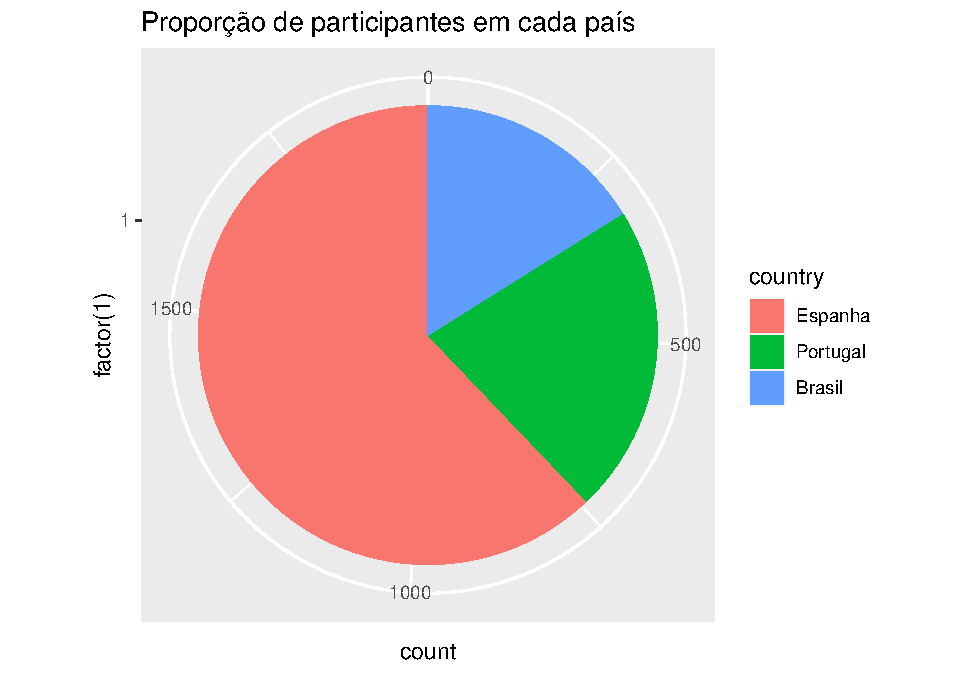
\includegraphics{gitbook-demo_files/figure-latex/unnamed-chunk-15-1} \end{center}

Esse gráfico permite um primeiro entendimento da distribuição dos dados. No entanto, a simples contagem de valores pode gerar uma percepção diferente caso a pesquisa tenha muitos ou poucos sujeitos. Para evitar isso, sugere-se a apresentar as proporções em vez das contagens.

A mudança da contagem para proporções pode ser feita por um recurso do pacote \texttt{scales}. A adição dos valores textuais às colunas tende e auxiliar a visualização.

\begin{Shaded}
\begin{Highlighting}[]
\KeywordTok{ggplot}\NormalTok{(Dataset, }\KeywordTok{aes}\NormalTok{(}\DataTypeTok{x =}\NormalTok{ country, }\DataTypeTok{y =}\NormalTok{ ..prop.., }\DataTypeTok{group =} \DecValTok{1}\NormalTok{)) }\OperatorTok{+}\StringTok{ }
\StringTok{  }\KeywordTok{geom_bar}\NormalTok{(}\DataTypeTok{stat =} \StringTok{"count"}\NormalTok{) }\OperatorTok{+}
\StringTok{  }\KeywordTok{geom_text}\NormalTok{(}\KeywordTok{aes}\NormalTok{(}\DataTypeTok{label=}\NormalTok{scales}\OperatorTok{::}\KeywordTok{percent}\NormalTok{(}\KeywordTok{round}\NormalTok{(..prop..,}\DecValTok{2}\NormalTok{)), }
                \DataTypeTok{y=}\NormalTok{..prop..), }\DataTypeTok{stat=} \StringTok{"count"}\NormalTok{, }\DataTypeTok{color =} \StringTok{"white"}\NormalTok{, }\DataTypeTok{size =} \DecValTok{3}\NormalTok{, }\DataTypeTok{position =} \KeywordTok{position_stack}\NormalTok{(}\DataTypeTok{vjust =} \FloatTok{0.5}\NormalTok{)) }\OperatorTok{+}
\StringTok{  }\KeywordTok{scale_y_continuous}\NormalTok{(}\DataTypeTok{labels =}\NormalTok{ scales}\OperatorTok{::}\KeywordTok{percent_format}\NormalTok{()) }\OperatorTok{+}
\StringTok{  }\KeywordTok{labs}\NormalTok{(}\DataTypeTok{x =} \StringTok{"País"}\NormalTok{, }\DataTypeTok{title =} \StringTok{"Proporção de participantes em cada país investigado"}\NormalTok{)}
\end{Highlighting}
\end{Shaded}

\begin{center}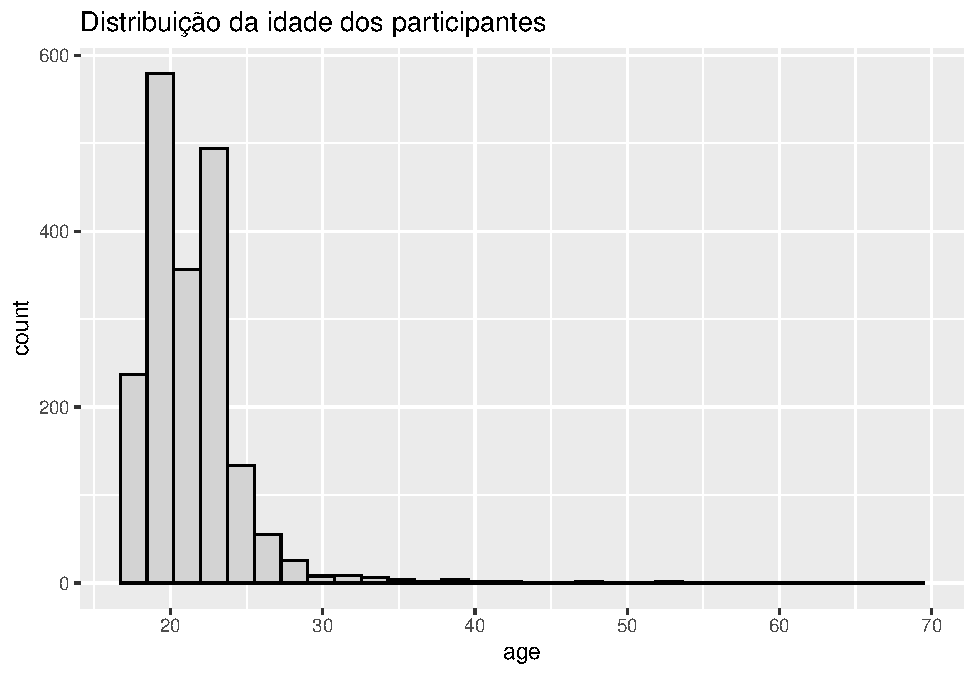
\includegraphics{gitbook-demo_files/figure-latex/unnamed-chunk-16-1} \end{center}

O gráfico de setor (as vezes chamado de polar, pizza ou torta) é também uma opção. O aspecto principal desse gráfico é o tamanho proporcional dos segmentos.

\begin{Shaded}
\begin{Highlighting}[]
\NormalTok{Dataset }\OperatorTok\StringTok{ }
\StringTok{  }\KeywordTok{count}\NormalTok{(country) }\OperatorTok\StringTok{ }
\StringTok{  }\KeywordTok{mutate}\NormalTok{(}\DataTypeTok{pct =}\NormalTok{ n}\OperatorTok{/}\KeywordTok{sum}\NormalTok{(n)) }\OperatorTok\StringTok{ }
\StringTok{  }\KeywordTok{ggplot}\NormalTok{(., }\KeywordTok{aes}\NormalTok{(}\DataTypeTok{x=}\StringTok{""}\NormalTok{, }\DataTypeTok{y=}\NormalTok{ pct, }\DataTypeTok{fill=}\NormalTok{country)) }\OperatorTok{+}
\StringTok{  }\KeywordTok{geom_col}\NormalTok{() }\OperatorTok{+}
\StringTok{  }\KeywordTok{geom_text}\NormalTok{(}\KeywordTok{aes}\NormalTok{(}\DataTypeTok{label =}\NormalTok{ scales}\OperatorTok{::}\KeywordTok{percent}\NormalTok{(}\KeywordTok{round}\NormalTok{(pct,}\DecValTok{3}\NormalTok{))), }\DataTypeTok{position =} \KeywordTok{position_stack}\NormalTok{(}\DataTypeTok{vjust =} \FloatTok{0.5}\NormalTok{))}\OperatorTok{+}
\StringTok{  }\KeywordTok{coord_polar}\NormalTok{(}\DataTypeTok{theta =} \StringTok{"y"}\NormalTok{) }\OperatorTok{+}
\StringTok{  }\KeywordTok{labs}\NormalTok{(}\DataTypeTok{title =} \StringTok{"Proporção de participantes em cada país"}\NormalTok{)}
\end{Highlighting}
\end{Shaded}

\begin{center}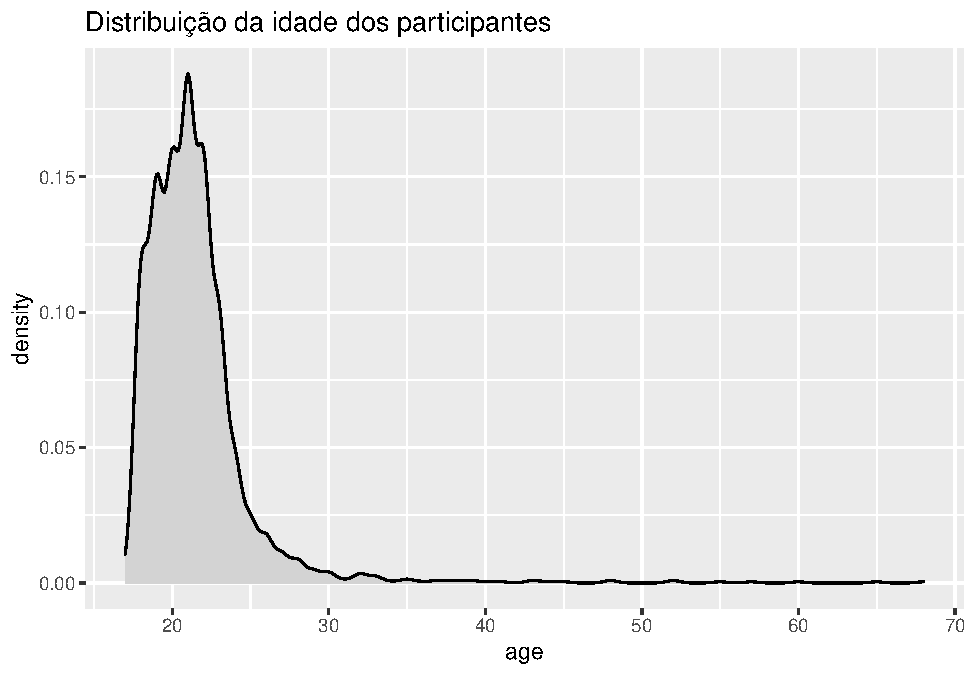
\includegraphics{gitbook-demo_files/figure-latex/unnamed-chunk-17-1} \end{center}

\hypertarget{variuxe1vel-contuxednua}{%
\section{1 variável contínua}\label{variuxe1vel-contuxednua}}

Quando uma única variável deve ser apresentada e ela é continua, os melhores gráficos para apresentar a distribuição dos dados são o histograma, densidade (kernel) e o boxplot.

Abaixo um histograma da idade dos participantes.

\begin{Shaded}
\begin{Highlighting}[]
\KeywordTok{ggplot}\NormalTok{(Dataset, }\KeywordTok{aes}\NormalTok{(}\DataTypeTok{x =}\NormalTok{ age)) }\OperatorTok{+}
\StringTok{  }\KeywordTok{geom_histogram}\NormalTok{(}\DataTypeTok{bins =} \DecValTok{30}\NormalTok{, }\DataTypeTok{color =} \StringTok{"black"}\NormalTok{, }\DataTypeTok{fill =} \StringTok{"#56B4E9"}\NormalTok{) }\OperatorTok{+}
\StringTok{  }\KeywordTok{labs}\NormalTok{(}\DataTypeTok{title =} \StringTok{"Distribuição da idade dos participantes"}\NormalTok{)}
\end{Highlighting}
\end{Shaded}

\begin{center}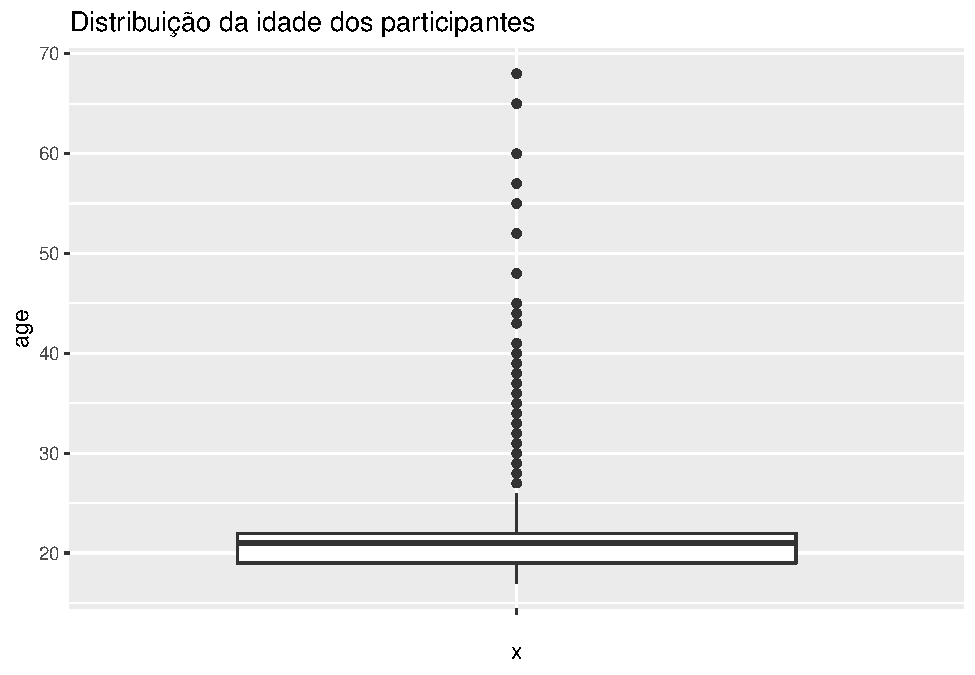
\includegraphics{gitbook-demo_files/figure-latex/unnamed-chunk-18-1} \end{center}

O histograma é formado por diversas barras unidas, possibilitando ter um entendimento dos intervalos entre cada um dos valores.

Abaixo um gráfico de densidade da idade:

\begin{Shaded}
\begin{Highlighting}[]
\KeywordTok{ggplot}\NormalTok{(Dataset, }\KeywordTok{aes}\NormalTok{(}\DataTypeTok{x =}\NormalTok{ age)) }\OperatorTok{+}
\StringTok{  }\KeywordTok{geom_density}\NormalTok{(}\DataTypeTok{fill =} \StringTok{"#56B4E9"}\NormalTok{) }\OperatorTok{+}
\StringTok{  }\KeywordTok{labs}\NormalTok{(}\DataTypeTok{title =} \StringTok{"Distribuição da idade dos participantes"}\NormalTok{)}
\end{Highlighting}
\end{Shaded}

\begin{center}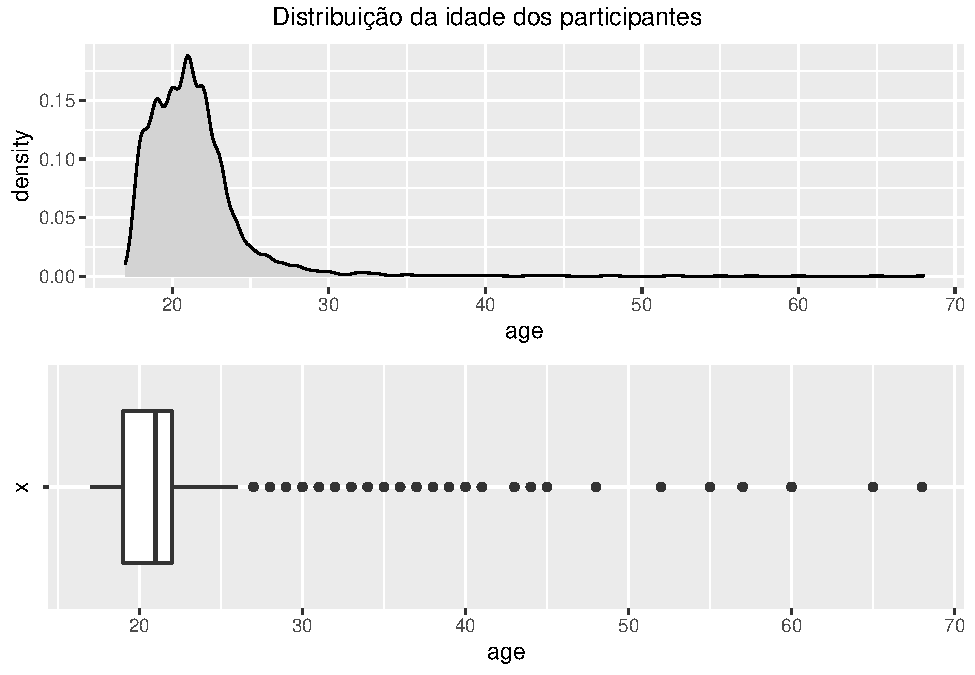
\includegraphics{gitbook-demo_files/figure-latex/unnamed-chunk-19-1} \end{center}

De maneira um pouco distinta do histograma, o gráfico de densidade ajusta uma curva aos dados. Com isso, este gráfico permite explorar a distribuição de probabilidade subjacente aos dados, o que será discutido futuramente.

Todas as distribuições de variáveis possuem uma localização, uma dispersão e um formato. De uma maneira mais direta, tanto o histograma como o gráfico de densidade retratam bem o formato da distribuição. Nesse caso, trata-se de uma assimetria positiva ou à direita. Esse tipo de assimetria é reconhecido pela cauda arrastada à direita.

Por sua vez, o boxplot dessa mesma variável pode ser criado:

\begin{Shaded}
\begin{Highlighting}[]
\KeywordTok{ggplot}\NormalTok{(Dataset, }\KeywordTok{aes}\NormalTok{(}\DataTypeTok{y =}\NormalTok{ age, }\DataTypeTok{x =} \StringTok{""}\NormalTok{)) }\OperatorTok{+}
\StringTok{  }\KeywordTok{geom_boxplot}\NormalTok{(}\DataTypeTok{fill =} \StringTok{"#56B4E9"}\NormalTok{) }\OperatorTok{+}
\StringTok{  }\KeywordTok{labs}\NormalTok{(}\DataTypeTok{title =} \StringTok{"Distribuição da idade dos participantes"}\NormalTok{)}
\end{Highlighting}
\end{Shaded}

\begin{center}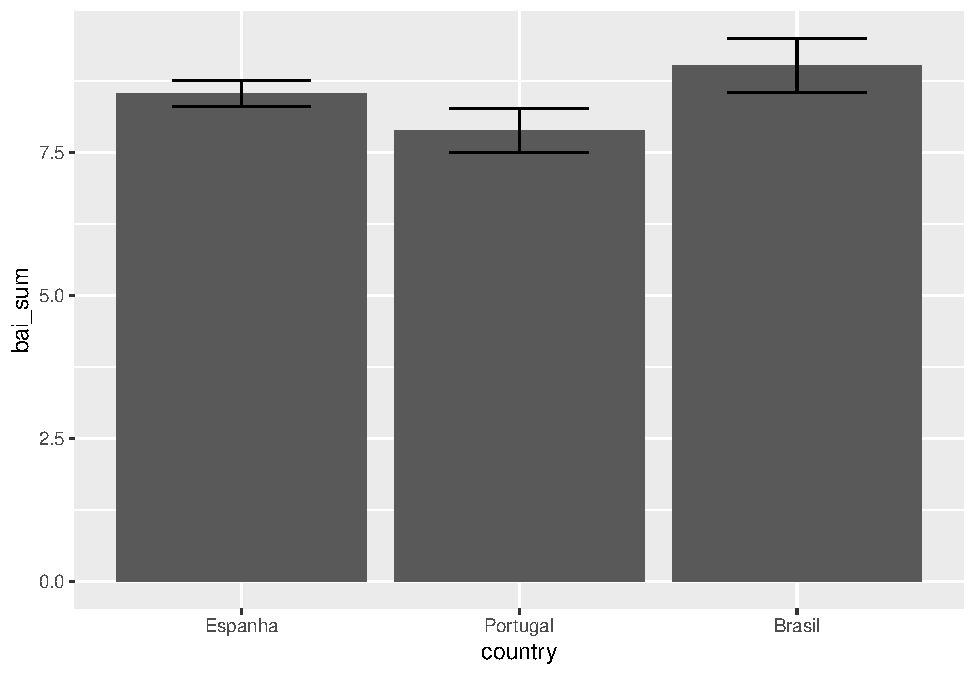
\includegraphics{gitbook-demo_files/figure-latex/unnamed-chunk-20-1} \end{center}

O boxplot é também chamado de ``diagrama de caixa e bigode'' e foi desenvolvido pelo matemático John W. Tukey na década de 1960. Este gráfico apresenta vantagens em comparação com os outros apresentados até agora, que são:

\begin{itemize}
\tightlist
\item
  Ele apresenta o formato da distribuição,\\
\item
  Na parte inferior da caixa, ele apresenta o valor do primeiro quartil, indicando os 25\% dos dados abaixo ou até ele,\\
\item
  Na linha mais espessa dentro da caixa, ele apresenta a mediana dos resultados (ou segundo quartil),\\
\item
  Na parte superior da caixa, ele apresenta o valor do terceiro quartil, indicando os 75\% dos dados que abaixo ou até ele,\\
\item
  A área da caixa apresenta 50\% dos dados, que estão situados entre o primeiro e o terceiro quartil,\\
\item
  As linhas abaixo e acima da caixa são chamadas de bigodes e indicam os valores mínimos e máximos sem considerar dados anômalos ou \emph{outliers},\\
\item
  Os valores acima ou abaixo das linhas indicam dados anômalos.
\end{itemize}

O cálculo da linha vertical que forma o bigode do gráfico é feito por \texttt{Q1\ -\ 1.5*IQR} e \texttt{Q3\ +\ 1.5*IQR}. Considera-se que os valores acima ou abaixo deste ponto são anômalos. Por definição, os \emph{outliers} são sempre poucos, mesmo que isso possa ser um pouco contraintuitivo nesta apresentação de agora.

Apesar de ser um pouco difícil de se visualizar ao início, os resultados apresentados nesses três gráficos são os mesmos, tal como demonstrado a seguir.

\begin{Shaded}
\begin{Highlighting}[]
\NormalTok{gridExtra}\OperatorTok{::}\KeywordTok{grid.arrange}\NormalTok{(}
  \CommentTok{#Grafico 1}
  \KeywordTok{ggplot}\NormalTok{(Dataset, }\KeywordTok{aes}\NormalTok{(}\DataTypeTok{x =}\NormalTok{ age)) }\OperatorTok{+}
\StringTok{    }\KeywordTok{geom_histogram}\NormalTok{(}\KeywordTok{aes}\NormalTok{(}\DataTypeTok{y=}\NormalTok{..density..), }\DataTypeTok{alpha=}\FloatTok{0.5}\NormalTok{, }
                   \DataTypeTok{position=}\StringTok{"identity"}\NormalTok{) }\OperatorTok{+}\StringTok{ }
\StringTok{    }\KeywordTok{geom_density}\NormalTok{(}\DataTypeTok{alpha=}\NormalTok{.}\DecValTok{8}\NormalTok{, }\DataTypeTok{fill =} \StringTok{"#56B4E9"}\NormalTok{),}
  \CommentTok{#Grafico 2}
  \KeywordTok{ggplot}\NormalTok{(Dataset, }\KeywordTok{aes}\NormalTok{(}\DataTypeTok{y =}\NormalTok{ age, }\DataTypeTok{x =} \StringTok{""}\NormalTok{)) }\OperatorTok{+}
\StringTok{  }\KeywordTok{geom_boxplot}\NormalTok{(}\DataTypeTok{fill =} \StringTok{"#56B4E9"}\NormalTok{) }\OperatorTok{+}\StringTok{ }\KeywordTok{labs}\NormalTok{(}\DataTypeTok{x =} \StringTok{""}\NormalTok{) }\OperatorTok{+}
\StringTok{  }\KeywordTok{coord_flip}\NormalTok{(),}
  \DataTypeTok{top =} \StringTok{"Distribuição da idade dos participantes"} \CommentTok{#título}
\NormalTok{)}
\end{Highlighting}
\end{Shaded}

\begin{center}\includegraphics{gitbook-demo_files/figure-latex/unnamed-chunk-21-1} \end{center}

\hypertarget{variuxe1veis-com-vi-discreta-e-vd-contuxednua}{%
\section{2 variáveis com VI discreta (e VD contínua)}\label{variuxe1veis-com-vi-discreta-e-vd-contuxednua}}

Quando duas variáveis são apresentadas, os gráficos permitem explorar diferenças entre grupos ou relação entre variáveis. Quando a VI é discreta, gráficos de barras, colunas ou boxplots apresentam as diferenças entre os grupos.

O gráfico de colunas abaixo apresenta os resultados médios do Inventário Beck de Ansiedade nos 3 países investigados.

\begin{Shaded}
\begin{Highlighting}[]
\KeywordTok{ggplot}\NormalTok{(Dataset, }\KeywordTok{aes}\NormalTok{(}\DataTypeTok{x =}\NormalTok{ country, }\DataTypeTok{y =}\NormalTok{ bai_sum)) }\OperatorTok{+}
\StringTok{  }\KeywordTok{geom_bar}\NormalTok{(}\DataTypeTok{stat =} \StringTok{"summary"}\NormalTok{, }\DataTypeTok{fun =}\NormalTok{ mean,}\DataTypeTok{fill =} \StringTok{"#56B4E9"}\NormalTok{) }
\end{Highlighting}
\end{Shaded}

\begin{center}\includegraphics{gitbook-demo_files/figure-latex/unnamed-chunk-22-1} \end{center}

Tal como exposto, é possível adicionar outros elementos a este gráfico para que uma primeira apreensão inferencial seja possível. Nesse sentido, o gráfico abaixo apresenta também as barras de erro.

\begin{Shaded}
\begin{Highlighting}[]
\KeywordTok{ggplot}\NormalTok{(Dataset, }\KeywordTok{aes}\NormalTok{(}\DataTypeTok{x =}\NormalTok{ country, }\DataTypeTok{y =}\NormalTok{ bai_sum)) }\OperatorTok{+}
\StringTok{  }\KeywordTok{geom_bar}\NormalTok{(}\DataTypeTok{stat =} \StringTok{"summary"}\NormalTok{, }\DataTypeTok{fun =}\NormalTok{ mean,}\DataTypeTok{fill =} \StringTok{"#56B4E9"}\NormalTok{) }\OperatorTok{+}
\StringTok{  }\KeywordTok{stat_summary}\NormalTok{(}\DataTypeTok{geom =} \StringTok{"errorbar"}\NormalTok{,}\DataTypeTok{fun.data =}\NormalTok{ mean_se, }\DataTypeTok{width =} \FloatTok{.5}\NormalTok{) }
\end{Highlighting}
\end{Shaded}

\begin{center}\includegraphics{gitbook-demo_files/figure-latex/unnamed-chunk-23-1} \end{center}

O boxplot a seguir também é um gráfico indicado. É importante notar que esse gráfico, em um primeiro momento, não traz informações sobre a média dos grupos, mas sim sobre a distribuição dos resultados. No entanto, como esse gráfico é bastante informativo, uma primeira noção inferencial já pode também ser feita.

\begin{Shaded}
\begin{Highlighting}[]
\KeywordTok{ggplot}\NormalTok{(Dataset, }\KeywordTok{aes}\NormalTok{(}\DataTypeTok{x =}\NormalTok{ country, }\DataTypeTok{y =}\NormalTok{ bai_sum)) }\OperatorTok{+}
\StringTok{  }\KeywordTok{geom_boxplot}\NormalTok{(}\DataTypeTok{fill =} \StringTok{"#56B4E9"}\NormalTok{)}
\end{Highlighting}
\end{Shaded}

\begin{center}\includegraphics{gitbook-demo_files/figure-latex/unnamed-chunk-24-1} \end{center}

\hypertarget{variuxe1veis-com-vi-contuxednua-e-vd-contuxednua}{%
\section{2 variáveis com VI contínua (e VD contínua)}\label{variuxe1veis-com-vi-contuxednua-e-vd-contuxednua}}

Quando tanto a VI como a VD são contínuas, os gráficos apresentam a relação entre as variáveis. Tanto o gráfico de pontos como o de dispersão são indicados, uma vez que eles são virtualmente idênticos No \texttt{ggplot}, o argumento \texttt{geom\_point} (à esquerda) e \texttt{geom\_jitter} (à direita) são possíveis.

\begin{Shaded}
\begin{Highlighting}[]
\NormalTok{gridExtra}\OperatorTok{::}\KeywordTok{grid.arrange}\NormalTok{(}
  \CommentTok{#Grafico 1}
  \KeywordTok{ggplot}\NormalTok{(Dataset, }\KeywordTok{aes}\NormalTok{(}\DataTypeTok{x =}\NormalTok{ age, }\DataTypeTok{y =}\NormalTok{ bai_sum)) }\OperatorTok{+}
\StringTok{  }\KeywordTok{geom_point}\NormalTok{(}\DataTypeTok{color =} \StringTok{"#56B4E9"}\NormalTok{),}

  \CommentTok{#Grafico 2}
  \KeywordTok{ggplot}\NormalTok{(Dataset, }\KeywordTok{aes}\NormalTok{(}\DataTypeTok{x =}\NormalTok{ age, }\DataTypeTok{y =}\NormalTok{ bai_sum)) }\OperatorTok{+}
\StringTok{  }\KeywordTok{geom_jitter}\NormalTok{(}\DataTypeTok{color=} \StringTok{"#56B4E9"}\NormalTok{),}
  \DataTypeTok{nrow=}\DecValTok{1}
\NormalTok{)}
\end{Highlighting}
\end{Shaded}

\begin{center}\includegraphics{gitbook-demo_files/figure-latex/unnamed-chunk-25-1} \end{center}

De maneira análoga aos elementos extras que podem ser apresentados em gráficos com VIs discretas, uma reta de regressão amostral (FRA) costuma ser adicionadas em gráficos em que a VI é contínua. Essa reta oferece uma primeira apreensão inferencial. No capítulo sobre modelos de regressão, esse conceito será novamente revisitado. A seguir, segue um exemplo.

\begin{Shaded}
\begin{Highlighting}[]
\KeywordTok{ggplot}\NormalTok{(Dataset, }\KeywordTok{aes}\NormalTok{(}\DataTypeTok{x =}\NormalTok{ age, }\DataTypeTok{y =}\NormalTok{ bai_sum)) }\OperatorTok{+}
\StringTok{  }\KeywordTok{geom_jitter}\NormalTok{(}\DataTypeTok{color =} \StringTok{"#56B4E9"}\NormalTok{) }\OperatorTok{+}
\StringTok{  }\KeywordTok{geom_smooth}\NormalTok{(}\DataTypeTok{method =} \StringTok{"lm"}\NormalTok{)}
\end{Highlighting}
\end{Shaded}

\begin{center}\includegraphics{gitbook-demo_files/figure-latex/unnamed-chunk-26-1} \end{center}

\hypertarget{outros-gruxe1ficos-e-configurauxe7uxf5es}{%
\section{Outros gráficos e configurações}\label{outros-gruxe1ficos-e-configurauxe7uxf5es}}

Os gráficos demonstrados costumam a ser os mais frequentes. Entretanto, é possível construir gráficos com uma maior complexidade, que reúnam diversas variáveis ao mesmo tempo. Evidentemente, a realização destes gráficos só tem sentido quando eles são relacionados ao problema de pesquisa estudado e não sobrecarreguem ou distorçam a visualização e entendimento dos resultados.

Frequentemente, essas informações adicionais são feitas pela inclusão de clusters ou agrupamentos. Isso é tanto possível em gráficos cuja VI seja discreta quanto contínua.

No exemplo abaixo, o gráfico dos resultados do Inventário Beck de Ansiedade entre os 3 países investigados (VI discreta) agora está agrupado pelo sexo do participante.

\begin{Shaded}
\begin{Highlighting}[]
\NormalTok{Dataset }\OperatorTok\StringTok{ }
\StringTok{  }\KeywordTok{filter}\NormalTok{(}\OperatorTok{!}\KeywordTok{is.na}\NormalTok{(sex)) }\OperatorTok\StringTok{ }
\StringTok{  }\KeywordTok{ggplot}\NormalTok{(., }\KeywordTok{aes}\NormalTok{(}\DataTypeTok{x =}\NormalTok{ country, }\DataTypeTok{y =}\NormalTok{ bai_sum, }\DataTypeTok{fill =}\NormalTok{ sex)) }\OperatorTok{+}
\StringTok{  }\KeywordTok{geom_bar}\NormalTok{(}\DataTypeTok{stat =} \StringTok{"summary"}\NormalTok{, }\DataTypeTok{position =} \StringTok{"dodge"}\NormalTok{) }\OperatorTok{+}
\StringTok{  }\KeywordTok{stat_summary}\NormalTok{(}\DataTypeTok{geom=}\StringTok{"errorbar"}\NormalTok{, }\DataTypeTok{fun.data =}\NormalTok{ mean_se, }\DataTypeTok{position =} \KeywordTok{position_dodge}\NormalTok{(}\FloatTok{0.95}\NormalTok{), }\DataTypeTok{width =} \FloatTok{.5}\NormalTok{) }
\end{Highlighting}
\end{Shaded}

\begin{center}\includegraphics{gitbook-demo_files/figure-latex/unnamed-chunk-27-1} \end{center}

Este gráfico traz uma informação importante sobre os resultados de homens e mulheres nos três países. Além disso, as barras de erro ajudam em um primeiro entendimento de possíveis diferenças significativas. Esse conceito irá ser revisitado em capítulos subsequentes.

No exemplo abaixo, a relação entre idade e pontuação no Inventário Beck de Ansiedade está agora agrupada pelo sexo do participante.

\begin{Shaded}
\begin{Highlighting}[]
\NormalTok{Dataset }\OperatorTok\StringTok{ }
\StringTok{  }\KeywordTok{filter}\NormalTok{(}\OperatorTok{!}\KeywordTok{is.na}\NormalTok{(sex)) }\OperatorTok\StringTok{ }
\StringTok{  }\KeywordTok{ggplot}\NormalTok{(., }\KeywordTok{aes}\NormalTok{(}\DataTypeTok{x =}\NormalTok{ age, }\DataTypeTok{y =}\NormalTok{ bai_sum, }\DataTypeTok{color =}\NormalTok{ sex)) }\OperatorTok{+}
\StringTok{  }\KeywordTok{geom_jitter}\NormalTok{() }\OperatorTok{+}
\StringTok{  }\KeywordTok{geom_smooth}\NormalTok{(}\DataTypeTok{method =} \StringTok{"lm"}\NormalTok{) }
\end{Highlighting}
\end{Shaded}

\begin{center}\includegraphics{gitbook-demo_files/figure-latex/unnamed-chunk-28-1} \end{center}

Neste gráfico de agora, é possível perceber que os a relação entre a idade e os resultados do Inventário Beck de Ansiedade é muito pequena e isso parece valer tanto para homens como para mulheres. Especialmente no capítulo de correlação, esse assunto será revisitado e parte dos termos utilizados aqui será alterado.

Por sua vez, situações em que há uma grande quantidade de variáveis apresentadas tendem a tornar os resultados difíceis de serem entendidos. O gráfico abaixo tenta traduzir essa condição, criando uma visualização de difícil entendimento justamente pelo excesso de variáveis presentes.

\begin{Shaded}
\begin{Highlighting}[]
\NormalTok{Dataset }\OperatorTok\StringTok{ }
\StringTok{  }\KeywordTok{filter}\NormalTok{(}\OperatorTok{!}\KeywordTok{is.na}\NormalTok{(sex), }\OperatorTok{!}\KeywordTok{is.na}\NormalTok{(curso_ou_ano)) }\OperatorTok\StringTok{ }
\StringTok{  }\KeywordTok{ggplot}\NormalTok{(., }\KeywordTok{aes}\NormalTok{(}\DataTypeTok{x =}\NormalTok{ age, }\DataTypeTok{y =}\NormalTok{ bai_sum, }\DataTypeTok{fill =} \KeywordTok{factor}\NormalTok{(curso_ou_ano), }\DataTypeTok{color =}\NormalTok{ sex, }\DataTypeTok{shape =}\NormalTok{ country)) }\OperatorTok{+}
\StringTok{  }\KeywordTok{geom_jitter}\NormalTok{() }\OperatorTok{+}
\StringTok{  }\KeywordTok{geom_smooth}\NormalTok{(}\DataTypeTok{method =} \StringTok{"lm"}\NormalTok{) }
\end{Highlighting}
\end{Shaded}

\begin{center}\includegraphics{gitbook-demo_files/figure-latex/unnamed-chunk-29-1} \end{center}

Espera-se que seja possível constatar que este gráfico é totalmente inadequado. Ele é carregado de informações, permite um baixo entendimento dos resultados da pesquisa e, eventualmente, pode gerar conclusões incorretas ou viesadas.

\hypertarget{execuuxe7uxe3o-no-jasp}{%
\section{Execução no JASP}\label{execuuxe7uxe3o-no-jasp}}

Da mesma forma que feito no R, será necessário carregar a base para o JASP. Durante todos os capítulos, esse procedimento de importação será requisitado.

\hypertarget{tabelas-1}{%
\section{Tabelas}\label{tabelas-1}}

Após ter a base disposta no JASP, para gerar tabelas e gráficos, será necessário acessar a opção \texttt{Descriptives}. O JASP tratará todas as variáveis com um símbolo de diagrama de venn ou barras como categóricas e todas as variáveis com símbolo de régua como contínuas.

\includegraphics{./img/cap_desc_jasp_descritivo.png}

Ao clicar nesta opção, será possível eleger as variáveis que irão ser analisadas e as variáveis que irão funcionar como agrupadores. Na prática, quando há duas ou mais variáveis para serem analisadas, a lista \texttt{Variables} irá reunir as variáveis dependentes, enquanto a variável independente será colocada na seção \texttt{Split}. É importante atentar à opção \texttt{Frequency\ tables\ (nominal\ and\ ordinal)}, que deve ser marcada quando o nível de medida da variável de interesse for nominal ou ordinal.

\includegraphics{./img/cap_desc_jasp_descritivo2.png}

Isto posto, as análises feitas no ambiente R serão parcialmente reproduzidas.

Inicialmente, uma tabela descrevendo os participantes em cada um dos país é importante para apresentar ao leitor algumas das principais características da amostra. Para fazer isso, será necessário levar a variável country para a seção \texttt{Variables} e clicar em \texttt{Frequency\ tables\ (nominal\ and\ ordinal)}.

\includegraphics{./img/cap_desc_jasp_proporcao.png}

Por padrão o JASP irá apresentar as contagens (frequências absolutas) e as proporções. A parte mais à esquerda da tabela descreverá os dados considerando todos os valores presentes na base. A parte mais à direita irá apresentar apenas os dados válidos, que não consideram casos ausentes. É importante atentar que o JASP não exclui estes casos. Ele apenas não os mostra.

Para verificar a frequência e a proporção de homens e mulheres na amostra, será necessário colocar também a variável sex na opção \texttt{Variables}. Não é preciso retirar a variável country antes de fazer isso. O JASP irá apresentar ambas as tabelas de maneira empilhada.

\includegraphics{./img/cap_desc_jasp_proporcao_duas_variaveis.png}

Para fazer uma tabela agrupando tanto country, como sex, é necessário arrastar uma das variáveis que estão em \texttt{Variables} para o espaço \texttt{Split}.

Em uma tabela em que se descreve a contagem e porcentagem de homens e mulheres em cada um dos três países de maneira independente, é necessário preencher o \texttt{Split} com a variável country. O JASP aceita que se arraste a variável de um local para o outro e, ao fazer isso, todas as contas serão automaticamente atualizadas.

\includegraphics{./img/cap_desc_jasp_proporcao_duas_variaveis_split.png}

É possível perceber que as variáveis categóricas são descritas por suas frequências e proporções. Por sua vez, variáveis contínuas costumam ser resumidas por medidas de posição e dispersão, tal como a média e o desvio-padrão. Como exemplo, para calcular tais medidas estatísticas dos valores do BDI e do BAI em função do país do participante, é necessário deixar a variável country em \texttt{Split} e levar as variáveis bdi\_sum e bai\_sum para \texttt{Variables}.

\includegraphics{./img/cap_desc_jasp_proporcao_duas_variaveis_split2.png}

Dessa vez, não é necessário ativar a opção \texttt{Frequency\ tables\ (nominal\ and\ ordinal)}. O símbolo de régua ao lado das variáveis bdi\_sum e bai\_sum indicam que elas são contínuas. O símbolo de diagrama de Venn ao lado de country, por sua vez, indica que ela é categórica.

Para fazer essas análises considerando sex como agrupador, será necessário substituir country por sex no espaço de \texttt{Split}.

\includegraphics{./img/cap_desc_jasp_proporcao_duas_variaveis_split3.png}

Nesta versão do JASP, não é possível colocar duas variáveis como agrupadoras. Dessa maneira, a reprodução das tabelas feitas anteriormente no ambiente R é apenas parcial.

\hypertarget{gruxe1ficos-2}{%
\section{Gráficos}\label{gruxe1ficos-2}}

O JASP é um excelente programa para gerar gráficos. Tal como previamente apresentado, a criação de um gráfico apropriado dependerá da finalidade desejada, bem como da quantidade de variáveis que devem ser apresentadas e o nível de medida da VI, especialmente em análises bi ou multivariadas.

O JASP pode fazer gráficos tanto seção \texttt{Descriptives} como após análise de dados específicas. Na seção \texttt{Descriptives}, será necessário primeiro arrastar as variáveis de interesse para seus respectivos lugares e, em seguida, clicar na opção \texttt{Plot}.

\includegraphics{./img/cap_desc_jasp_graficos.png}

\hypertarget{variuxe1vel-discreta-1}{%
\section{1 variável discreta}\label{variuxe1vel-discreta-1}}

Para este tipo de variável, gráfico de barras, colunas e setor são indicados. Para realizar um gráfico de barras, é necessário colocar a variável de interesse em \texttt{Variables} e, dentro de \texttt{Plots}, clicar em \texttt{Distribuiton\ plots}. O JASP organiza as barras de ordem crescente. No exemplo abaixo, a variável country é apresentada.

\includegraphics{./img/cap_desc_jasp_grafico_barras.png}

Para realizar um gráfico de setor, basta selecionar a opção \texttt{Pie\ Charts}. A visualização ocorrerá automaticamente. Uma vantagem deste gráfico é a apresentação proporcional dos elementos gráficos, em vez de contagens. Infelizmente, nesta versão do JASP, não é possível adicionar um rótulo com a porcentagem de cada categoria.

\includegraphics{./img/cap_desc_jasp_grafico_setor.png}

O JASP permite customizar as cores de alguns gráficos. Para fazer isso, basta clicar em \texttt{Color\ Palette} e escolher entre as opções disponíveis. Existem algumas possibilidades e recomendo optar por aquelas que permitem que pessoas com limitações visuais possam também se beneficiar. Entretanto, apenas como demonstração, o tema \texttt{ggplot2} é apresentado abaixo.

\includegraphics{./img/cap_desc_jasp_grafico_setor2.png}

\hypertarget{variuxe1vel-contuxednua-1}{%
\section{1 variável contínua}\label{variuxe1vel-contuxednua-1}}

Histogramas, gráficos de densidade e boxplots costumam ser indicados para variáveis contínuas. Para o JASP fazer tais gráficos, é necessário que o espaço \texttt{Variables} seja preenchido por alguma variável que tenha o símbolo da régua ao lado. A variável age é um bom exemplo.

Ao colocá-la neste local e marcar a opção \texttt{Distribution\ plots}, um histograma será automaticamente apresentado.

\includegraphics{./img/cap_desc_jasp_grafico_histograma.png}

É possível adicionar a densidade de maneira sobreposta ao histograma clicando em \texttt{Display\ density}. Ambos os gráficos são importantes para verificar o formato da distribuição dos dados. Neste caso, a distribuição é assimétrica à direita.

\includegraphics{./img/cap_desc_jasp_grafico_densidade.png}

Por sua vez, o boxplot pode ser criado ao se clicar na opção \texttt{Boxplots} e, em seguida, \texttt{Boxplot\ element}.

\includegraphics{./img/cap_desc_jasp_grafico_boxplot.png}

É possível customizar o boxplot. Além disso, o JASP permite criar outros gráficos que vêm sendo mais utilizados recentemente, como o gráfico de violino. Isso não será demonstrado aqui, mas para fazer isso, basta ativar as opções desejadas na seção \texttt{Customizable\ plots}.

Tal como discutido anteriormente, o boxplot apresenta vantagens em comparação com os outros gráficos apresentados até agora, que são:

\begin{itemize}
\tightlist
\item
  Ele apresenta o formato da distribuição,\\
\item
  Na parte inferior da caixa, ele apresenta o valor do primeiro quartil, indicando os 25\% dos dados abaixo ou até ele,\\
\item
  Na linha mais espessa dentro da caixa, ele apresenta a mediana dos resultados (ou segundo quartil),\\
\item
  Na parte superior da caixa, ele apresenta o valor do terceiro quartil, indicando os 75\% dos dados que abaixo ou até ele,\\
\item
  A área da caixa apresenta 50\% dos dados, que estão situados entre o primeiro e o terceiro quartil,\\
\item
  As linhas abaixo e acima da caixa são chamadas de bigodes e indicam os valores mínimos e máximos sem considerar dados anômalos ou \emph{outliers},\\
\item
  Os valores acima ou abaixo da linhas indicam dados anômalos.
\end{itemize}

\hypertarget{variuxe1veis-com-vi-discreta-e-vd-contuxednua-1}{%
\section{2 variáveis com VI discreta (e VD contínua)}\label{variuxe1veis-com-vi-discreta-e-vd-contuxednua-1}}

Para situações em que há duas variáveis, a VI é tratada como discreta e a VD é contínua, gráficos de barras, colunas ou boxplots são indicados. Esses gráficos permitem verificar diferenças entre grupos. Nesta versão do JASP, apenas o boxplot pode ser feito. Para verificar, por exemplo, a distribuição dos resultados do bai\_sum em função do país, é necessário levar às variáveis a seus respectivos locais e, em seguida, solicitar ao JASP o boxplot.

\includegraphics{./img/cap_desc_jasp_grafico_boxplot_grupo.png}

\hypertarget{variuxe1veis-com-vi-contuxednua-e-vd-contuxednua-1}{%
\section{2 variáveis com VI contínua (e VD contínua)}\label{variuxe1veis-com-vi-contuxednua-e-vd-contuxednua-1}}

Quando há duas variáveis contínuas, tanto o gráfico de pontos como de dispersão são possíveis. Esses gráficos permitem verificar o relacionamento entre variáveis. Para fazer isso, é necessário incluir ambas as variáveis de interesse para o espaço \texttt{Variables}. Por exemplo, age e bai\_sum.

\includegraphics{./img/cap_desc_jasp_grafico_scatter1.png}

Após clicar na opção \texttt{Plots}, é possível tanto marcar a opção \texttt{Scatter\ Plots}, como a opção \texttt{Correlation\ Plots}.

\includegraphics{./img/cap_desc_jasp_grafico_scatter2.png}

A escolha de cada gráfico é relacionada com os elementos que devem (ou não) serem incluídos na apresentação. Na opção \texttt{Scatter\ Plot}, o gráfico irá exibir os pontos dos respectivos pares ordenados das variáveis X e Y, suas densidades e também adicionar uma reta de regressão. Este último conceito será revisitado no capítulo de regressão.

Um aspecto visualmente importante é a eleição de qual variável irá em X. Com bastante frequência, deve-se inserir a VI (mesmo que teórica) em X, enquanto a VD em Y. Isso é feito alterando a ordem das variáveis em \texttt{Variables}.

\includegraphics{./img/cap_desc_jasp_grafico_scatter3.png}

\hypertarget{outros-gruxe1ficos-e-configurauxe7uxf5es-1}{%
\section{Outros gráficos e configurações}\label{outros-gruxe1ficos-e-configurauxe7uxf5es-1}}

O JASP é bastante versátil na realização de gráficos e permite que mais variáveis sejam inseridas. Há também um módulo (\texttt{Module}) chamado \texttt{Visual\ Modeling}, que permite uma grande customização de gráficos. Para acessá-lo, é necessário clicar na cruz azul, tal como destacado no quadrado roxo da imagem abaixo.

\includegraphics{./img/cap_desc_jasp_modules.png}

Na lista de opções, é necessário ativar \texttt{Visual\ Modeling}. Ao fazer isso, o ícone será ativado na barra de ferramentas.

\includegraphics{./img/cap_desc_jasp_visual_modeling.png}

Com isso feito, dentro de \texttt{Visual\ Modeling}, a opção \texttt{Flexplot} oferece uma melhora substancial aos gráficos que o JASP executa. Agora é possível, por exemplo, fazer um gráfico incluindo um cluster ou agrupamento, em que os resultados do Inventário Beck de Ansiedade são apresentados tanto em função dos países investigados, como do sexo do participante.

\includegraphics{./img/cap_desc_jasp_flexplot.png}

Uma série de outras opções e combinações podem ser feitas ao clicar em \texttt{Options} e \texttt{Plot\ Labels}. Elas não serão apresentadas nesta seção.

\hypertarget{resumo-2}{%
\section{Resumo}\label{resumo-2}}

Este capítulo apresentou os aspectos tabulares e gráficos corriqueiramente encontrados em pesquisas de Psicologia e áreas congêneres. Entre os pontos principais, estão os seguintes:

\begin{enumerate}
\def\labelenumi{\arabic{enumi}.}
\tightlist
\item
  Medidas de posição e dispersão são fundamentais na apresentação dos resultados de uma pesquisa\\
\item
  Variáveis categóricas são resumidas por contagens e proporções. Variáveis contínuas por suas médias e desvios-padrão\\
\item
  Tabelas e gráficos devem ser claros ao leitor, sem criar viés ou distorção dos resultados\\
\item
  As tabelas são muito úteis para uma apresentação detalhada dos resultados\\
\item
  Gráficos condensam um grande volume de dados de uma forma mais facilmente interpretável\\
\item
  A heurística típica em gráficos solicita responder a quantidade e a natureza das variáveis a serem apresentadas\\
\end{enumerate}

\hypertarget{questuxf5es-1}{%
\section{Questões}\label{questuxf5es-1}}

\begin{enumerate}
\def\labelenumi{\arabic{enumi}.}
\tightlist
\item
  Trata-se de um círculo dividido por fatias cujos ângulos internos são proporcionais às partes envolvidas. Este é um gráfico:a) De colunasb) Histogramac)De Setord) Boxplote)Barras
\item
  É uma medida de posição para variáveis propriamente numéricas e que é obtida somando-se todos os valores observados e dividindo-se o resultado pelo número de observaçõesa) Medianab) Médiac) Modad) Desvio-padrãoe) Amplitude interquartil
\item
  (ENADE, Biomedicina - 2010) Para apresentarem gráficos dados referentes à distribuição de frequências de um grupo de medições, pode-se aplicar um modelo semelhante ao estabelecido na figura abaixo, na qual o pesquisador verifica a variação de anticorpos em relação a uma coorte populacional específica.\includegraphics{./img/exercicio_histograma.png}a) Gráfico de setores, que demonstra a variação de anticorpos na abscissa Y e de população na ordenada X. b) Histograma, que demonstra variações de anticorpos na abscissa X e de população na ordenada Y c) Gráfico de tendência central, que demonstra variações de anticorpos na abscissa X e de população na ordenada Y. d) Gráficos de dispersão, que demonstra a tendência central das médias de concentração dos valores de anticorpos na população. e) Gráfico de linhas, que demonstra a tendência central baseada na mediana das concentrações de anticorpos na população.
\end{enumerate}

Gabarito: 1-c; 2-b; 3-b

\hypertarget{famuxedlia-de-distribuiuxe7uxf5es}{%
\chapter{Família de distribuições}\label{famuxedlia-de-distribuiuxe7uxf5es}}

\textbf{Objetivos do capítulo}\\
1. Introduzir aspectos voltados ao formato das distribuições\\
2. Apresentar a distribuição formal e suas características\\
3. Apresentar dados simulados para ilustrar a Lei dos Grandes Números e o Teorema Central do Limite

\emph{Parcialmente adaptado de Anunciação, Portugal, Landeira-Fernandez (2021). Aspectos psicométricos de instrumentos neuropsicológicos: revisão conceitual, proposta de interpretação de percentis e classificações }

Em estatística, uma variável aleatória é uma função que associa cada elemento de um dado espaço amostral a um número real (\(X:\Omega \rightarrow R\)). O mapeamento desses valores depende de um experimento aleatório, seguida pela análise do conjunto de valores obtidos, chamado de realizações. Apesar desses conceitos serem importantes, o atalho pedagógico utilizado para esta definição entende as variáveis como características que podem apresentar qualquer valor, tal como peso, inteligência e renda.

Todas as variáveis apresentam resultados numéricos que podem ser contínuos ou discretos. Esses resultados se distribuem de acordo com uma família de distribuições de probabilidades (que também podem ser discretas ou contínuas) e podem ser pragmaticamente apresentados por uma expressão analítica (uma fórmula), tabelas ou gráficos.

Os gráficos são muito úteis para indicar os três principais aspectos das distribuições, que são: a localização (ou centro), a dispersão e o formato. A tabela abaixo apresenta cada um desses componentes e uma definição.

\begin{longtable}[]{@{}llll@{}}
\toprule
\begin{minipage}[b]{0.22\columnwidth}\raggedright
Componente\strut
\end{minipage} & \begin{minipage}[b]{0.22\columnwidth}\raggedright
Definição\strut
\end{minipage} & \begin{minipage}[b]{0.22\columnwidth}\raggedright
Medida\strut
\end{minipage} & \begin{minipage}[b]{0.22\columnwidth}\raggedright
Gráfico\strut
\end{minipage}\tabularnewline
\midrule
\endhead
\begin{minipage}[t]{0.22\columnwidth}\raggedright
Localização\strut
\end{minipage} & \begin{minipage}[t]{0.22\columnwidth}\raggedright
Expressa o valor médio que está sendo observado\strut
\end{minipage} & \begin{minipage}[t]{0.22\columnwidth}\raggedright
Média, Moda e Mediana\strut
\end{minipage} & \begin{minipage}[t]{0.22\columnwidth}\raggedright
Histograma, Boxplot\strut
\end{minipage}\tabularnewline
\begin{minipage}[t]{0.22\columnwidth}\raggedright
Dispersão\strut
\end{minipage} & \begin{minipage}[t]{0.22\columnwidth}\raggedright
Expressa o afastamento do valor da localização\strut
\end{minipage} & \begin{minipage}[t]{0.22\columnwidth}\raggedright
Amplitude, Variância, Desvio-padrão, IQR\strut
\end{minipage} & \begin{minipage}[t]{0.22\columnwidth}\raggedright
Histograma, Boxplot\strut
\end{minipage}\tabularnewline
\begin{minipage}[t]{0.22\columnwidth}\raggedright
Formato\strut
\end{minipage} & \begin{minipage}[t]{0.22\columnwidth}\raggedright
Apresenta como a variação ocorre em função da localização\strut
\end{minipage} & \begin{minipage}[t]{0.22\columnwidth}\raggedright
Assimetria e curtose\strut
\end{minipage} & \begin{minipage}[t]{0.22\columnwidth}\raggedright
Histograma, Boxplot\strut
\end{minipage}\tabularnewline
\bottomrule
\end{longtable}

A localização e a dispersão foram trabalhadas no capítulo sobre estatística descritiva, que também apresentou resumidamente o Coeficiente de Assimetria e Curtose. Dessa maneira, o capítulo atual tem maior ênfase sobre os possíveis formatos de uma distribuição.

Em relação ao formato, as distribuições podem ser simétricas ou assimétricas. Quando assimétricas, a assimetria pode ser à direita ou à esquerda.

\hypertarget{distribuiuxe7uxe3o-simuxe9trica}{%
\section{Distribuição simétrica}\label{distribuiuxe7uxe3o-simuxe9trica}}

Este tipo de distribuição é simétrica em torno da média. Existem algumas famílias de probabilidade que apresentam formato similar a esse, que será melhor descrito a seguir, na seção sobre Distribuição normal.

Visualmente, a distribuição se apresenta da seguinte maneira:

\begin{center}\includegraphics{gitbook-demo_files/figure-latex/unnamed-chunk-31-1} \end{center}

\hypertarget{assimetria-uxe0-direita}{%
\section{Assimetria à direita}\label{assimetria-uxe0-direita}}

Este tipo de assimetria é marcada por caudas longas à direita. Em distribuições que obedecem a este padrão, os outliers ou pontos anômalos tem valores significativamente altos. Visualmente, esta distribuição tem o seguinte formato.

\begin{center}\includegraphics{gitbook-demo_files/figure-latex/unnamed-chunk-32-1} \end{center}

Entre as principais características, (1) a média é maior do que a mediana, (2) a quantidade de observações abaixo da média é superior à quantidade de observações acima da média e (3) o Coeficiente de Assimetria é positivo. No caso da imagem o valor é 1.1.

Entre as distribuições com este formato, estão a gamma e alguns casos particulares, como a exponencial e a qui-quadrado.

Exemplos reais: Tempo de espera em uma fila de banco, quilometragem de carros usados que estão à venda, tempo de reação em experimentos psicológicos, preço de casas à venda, número de acidentes de trânsito que uma pessoa se envolve durante um ano, quantidade de filhos que as famílias possuem.

\hypertarget{assimetria-uxe0-esquerda-ou-negativa}{%
\section{Assimetria à esquerda (ou negativa)}\label{assimetria-uxe0-esquerda-ou-negativa}}

Este tipo de assimetria é marcada por caudas longas à esquerda. Em distribuições que obedecem a este padrão, os outliers ou pontos anômalos tem valores significativamente baixos Visualmente, esta distribuição tem o seguinte formato.

\begin{center}\includegraphics{gitbook-demo_files/figure-latex/unnamed-chunk-33-1} \end{center}

Entre as principais características, (1) a média é menor do que a mediana, (2) a quantidade de observações abaixo da média é inferior à quantidade de observações acima da média e (3) o Coeficiente de Assimetria é negativo. No caso da imagem o valor é -0.9.

Exemplos reais: Idade da morte de brasileiros, quantidade de horas que as pessoas passam na internet, quantidade de dedos que a população tem nas mãos.

\hypertarget{a-distribuiuxe7uxe3o-normal}{%
\section{A distribuição normal}\label{a-distribuiuxe7uxe3o-normal}}

A distribuição normal é um tipo de distribuição simétrica, considerada a mais importante em estatística e que apresenta características visuais e analíticas marcantes. Seu formato é apresentado a seguir:

\begin{center}\includegraphics{gitbook-demo_files/figure-latex/unnamed-chunk-34-1} \end{center}

Em relação aos aspectos visuais:

\begin{enumerate}
\def\labelenumi{\arabic{enumi})}
\tightlist
\item
  Ela é simétrica,\\
\item
  Há um único pico e duas caudas, uma à esquerda e outra à direita (o que gera um formato de sino),\\
\item
  Apesar de contraintuitivo, essas caudas não se estendem infinitamente à esquerda e à direita.
\end{enumerate}

Em relação às características analíticas

\begin{enumerate}
\def\labelenumi{\arabic{enumi})}
\tightlist
\item
  Ela integra a família das distribuições contínuas (e, portanto, tem uma função densidade de probabilidade),
\item
  Ela é definida por dois parâmetros (média e variância), o que significa que é possível construir infinitas distribuições normais,\\
\item
  O ponto ao centro reúne o valor da média, moda e mediana, que são iguais,\\
\item
  O Coeficiente de Assimetria é igual a 0,\\
\item
  O Coeficiente de Curtose é igual a 3.
\end{enumerate}

\begin{center}\includegraphics{gitbook-demo_files/figure-latex/unnamed-chunk-35-1} \end{center}

Em Psicologia, os fenômenos psicológicos são assumidos como normais, motivo pela qual essa distribuição possui ainda mais importância na área.

Exemplos reais: Altura de homens/mulheres adultos(as), erros em equipamentos de medição em astronomia, pressão arterial de adultos, tamanho de bebês recém-nascidos.

\hypertarget{a-regra-empuxedrica}{%
\section{A regra empírica}\label{a-regra-empuxedrica}}

Uma característica importante da distribuição normal (e outras distribuições simétricas) é a regra empírica.

De com esta regra, em uma variável aleatória normalmente distribuída, cerca de 68\% das observações estará contida no intervalo de -1 a +1 desvio-padrão, cerca de 95\% das observações estará entre -2 e +2 desvios-padrão e carca de 99.7\% das observações estará entre -3 e +3 desvios-padrão.

A figura abaixo apresenta esta relação.

\begin{center}\includegraphics{gitbook-demo_files/figure-latex/unnamed-chunk-36-1} \end{center}

\hypertarget{um-resumo-visual}{%
\section{Um resumo visual}\label{um-resumo-visual}}

Este capítulo pode ser entendido de muitas maneiras. Elementos visuais tendem a gerar uma assimilação mais rápida e duradoura desses conteúdos. Abaixo, há três formatos de distribuição. O cachorro no meio ilustra uma distribuição simétrica. Nela, a área embaixo da curva decai da mesma forma com referência ao centro. O cachorro da esquerda ilustra uma assimetria negativa. Repare que o rabo dele está para o lado esquerdo. Por sua vez, o cachorro da direita ilustra uma assimetria à direita. Repare que o rabo dele, por sua vez, está ao lado direito.

\includegraphics{./img/cap_desc_assimetria.png}

\hypertarget{importuxe2ncia-inferencial}{%
\section{Importância inferencial}\label{importuxe2ncia-inferencial}}

Uma das principais atividades realizadas na estatística é a generalização de resultados obtidos em uma pesquisa à população de onde a amostra foi retirada. Este tema será melhor apresentado no capítulo de inferência.

\textbf{Atenção}: A Lei dos Grandes Números e o Teorema Central do Limite são dois pilares da teoria da probabilidade e de procedimentos inferenciais.

Duas teorias em estatística são muito importantes e impactam tanto no tamanho amostral como na utilização da distribuição normal em processos inferenciais, que são a Lei dos Grandes Números (LLN) e o Teorema Central do Limite (CLT).

Lei dos Grandes Números (LLN): Essa Lei é um teorema fundamental da teoria da probabilidade. De acordo com ela, a média aritmética dos resultados da realização da mesma experiência repetidas vezes tende a se aproximar do valor esperado à medida que mais tentativas se sucederem. Ou seja, a média amostral converge em probabilidade à média populacional.

Uma demonstração simples é feita pelo jogo de moedas. Sabe-se que há uma probabilidade de 50\% do resultado deste experimento ser cara, da mesma forma que há esta mesma probabilidade de ser coroa. É possível codificar cara como 1 e coroa como 0.

Se assumirmos que \(Sn\) o número de caras em \(n\) experimentos,há:

\[S_n = X_1 + X_2 + \dots + X_n\]

A proporção de caras é dada por:

\[R_n = \frac{S_n}{n}\]

Pela Lei dos Grandes Números, haverá uma convergência em probabilidade:

\[R_n \overset{p}{\to} p\quad quando \quad n \rightarrow \infty \]
Dados simulados apresentando os primeiros resultados são:

\begin{Shaded}
\begin{Highlighting}[]
\KeywordTok{head}\NormalTok{(lln) }\OperatorTok\StringTok{ }\NormalTok{pander}\OperatorTok{::}\KeywordTok{pander}\NormalTok{()}
\end{Highlighting}
\end{Shaded}

\begin{longtable}[]{@{}cccc@{}}
\toprule
\begin{minipage}[b]{0.16\columnwidth}\centering
lancamento\strut
\end{minipage} & \begin{minipage}[b]{0.15\columnwidth}\centering
resultado\strut
\end{minipage} & \begin{minipage}[b]{0.22\columnwidth}\centering
acumulado\_caras\strut
\end{minipage} & \begin{minipage}[b]{0.16\columnwidth}\centering
prob\_caras\strut
\end{minipage}\tabularnewline
\midrule
\endhead
\begin{minipage}[t]{0.16\columnwidth}\centering
1\strut
\end{minipage} & \begin{minipage}[t]{0.15\columnwidth}\centering
Cara\strut
\end{minipage} & \begin{minipage}[t]{0.22\columnwidth}\centering
1\strut
\end{minipage} & \begin{minipage}[t]{0.16\columnwidth}\centering
100\strut
\end{minipage}\tabularnewline
\begin{minipage}[t]{0.16\columnwidth}\centering
2\strut
\end{minipage} & \begin{minipage}[t]{0.15\columnwidth}\centering
Coroa\strut
\end{minipage} & \begin{minipage}[t]{0.22\columnwidth}\centering
1\strut
\end{minipage} & \begin{minipage}[t]{0.16\columnwidth}\centering
50\strut
\end{minipage}\tabularnewline
\begin{minipage}[t]{0.16\columnwidth}\centering
3\strut
\end{minipage} & \begin{minipage}[t]{0.15\columnwidth}\centering
Cara\strut
\end{minipage} & \begin{minipage}[t]{0.22\columnwidth}\centering
2\strut
\end{minipage} & \begin{minipage}[t]{0.16\columnwidth}\centering
66.67\strut
\end{minipage}\tabularnewline
\begin{minipage}[t]{0.16\columnwidth}\centering
4\strut
\end{minipage} & \begin{minipage}[t]{0.15\columnwidth}\centering
Cara\strut
\end{minipage} & \begin{minipage}[t]{0.22\columnwidth}\centering
3\strut
\end{minipage} & \begin{minipage}[t]{0.16\columnwidth}\centering
75\strut
\end{minipage}\tabularnewline
\begin{minipage}[t]{0.16\columnwidth}\centering
5\strut
\end{minipage} & \begin{minipage}[t]{0.15\columnwidth}\centering
Coroa\strut
\end{minipage} & \begin{minipage}[t]{0.22\columnwidth}\centering
3\strut
\end{minipage} & \begin{minipage}[t]{0.16\columnwidth}\centering
60\strut
\end{minipage}\tabularnewline
\begin{minipage}[t]{0.16\columnwidth}\centering
6\strut
\end{minipage} & \begin{minipage}[t]{0.15\columnwidth}\centering
Cara\strut
\end{minipage} & \begin{minipage}[t]{0.22\columnwidth}\centering
4\strut
\end{minipage} & \begin{minipage}[t]{0.16\columnwidth}\centering
66.67\strut
\end{minipage}\tabularnewline
\bottomrule
\end{longtable}

À medida que a quantidade de lançamentos aumenta, a probabilidade se aproxima à esperada, ilustrando a Lei dos Grandes Números. O gráfico a seguir demonstra esse resultado.

\begin{center}\includegraphics{gitbook-demo_files/figure-latex/unnamed-chunk-39-1} \end{center}

O Teorema Central do Limite (CLT): Se uma variável aleatória (por exemplo, X) puder ser representada pela soma de quaisquer \(n\) variáveis aleatórias independentes, que satisfaçam certas condições gerais, esta soma terá distribuição aproximadamente normal para \(n\) suficientemente grande.

Uma demonstração pode ser feita. Se um conjunto de pesquisas forem realizadas em uma variável cuja distribuição tenha formato uniforme, em cada uma das pesquisas (realizações), os resultados terão formato uniforme, tal como demonstrado a seguir:

\begin{center}\includegraphics{gitbook-demo_files/figure-latex/unnamed-chunk-40-1} \end{center}

Caso a média de cada uma das pesquisas (realizações) seja tirada e arquivada em um banco de dados, os 10 primeiros resultados serão os seguintes:

\begin{Shaded}
\begin{Highlighting}[]
\KeywordTok{head}\NormalTok{(clt_sample_means) }\OperatorTok\StringTok{ }\NormalTok{pander}\OperatorTok{::}\KeywordTok{pander}\NormalTok{()}
\end{Highlighting}
\end{Shaded}

\begin{longtable}[]{@{}cc@{}}
\toprule
\begin{minipage}[b]{0.13\columnwidth}\centering
samples\strut
\end{minipage} & \begin{minipage}[b]{0.13\columnwidth}\centering
means\strut
\end{minipage}\tabularnewline
\midrule
\endhead
\begin{minipage}[t]{0.13\columnwidth}\centering
1\strut
\end{minipage} & \begin{minipage}[t]{0.13\columnwidth}\centering
0.496\strut
\end{minipage}\tabularnewline
\begin{minipage}[t]{0.13\columnwidth}\centering
2\strut
\end{minipage} & \begin{minipage}[t]{0.13\columnwidth}\centering
0.4917\strut
\end{minipage}\tabularnewline
\begin{minipage}[t]{0.13\columnwidth}\centering
3\strut
\end{minipage} & \begin{minipage}[t]{0.13\columnwidth}\centering
0.5188\strut
\end{minipage}\tabularnewline
\begin{minipage}[t]{0.13\columnwidth}\centering
4\strut
\end{minipage} & \begin{minipage}[t]{0.13\columnwidth}\centering
0.4968\strut
\end{minipage}\tabularnewline
\begin{minipage}[t]{0.13\columnwidth}\centering
5\strut
\end{minipage} & \begin{minipage}[t]{0.13\columnwidth}\centering
0.5075\strut
\end{minipage}\tabularnewline
\begin{minipage}[t]{0.13\columnwidth}\centering
6\strut
\end{minipage} & \begin{minipage}[t]{0.13\columnwidth}\centering
0.5008\strut
\end{minipage}\tabularnewline
\bottomrule
\end{longtable}

A distribuição das médias das médias é, aproximadamente, normal.

\begin{Shaded}
\begin{Highlighting}[]
\KeywordTok{ggplot}\NormalTok{(clt_sample_means, }\KeywordTok{aes}\NormalTok{(}\DataTypeTok{x=}\NormalTok{means))}\OperatorTok{+}
\StringTok{  }\KeywordTok{geom_histogram}\NormalTok{(}\DataTypeTok{color=}\StringTok{"white"}\NormalTok{, }\DataTypeTok{bins=}\DecValTok{15}\NormalTok{)}\OperatorTok{+}
\StringTok{  }\KeywordTok{theme_classic}\NormalTok{()}
\end{Highlighting}
\end{Shaded}

\begin{center}\includegraphics{gitbook-demo_files/figure-latex/unnamed-chunk-43-1} \end{center}

\hypertarget{resumo-3}{%
\section{Resumo}\label{resumo-3}}

Este capítulo introduziu aspectos relacionados ao formato da distribuição das variáveis, com os seguintes pontos principais:

\begin{enumerate}
\def\labelenumi{\arabic{enumi}.}
\tightlist
\item
  Todas as variáveis se distribuem e o formato delas pode ser descrito de maneira analítica, tabular ou gráfica\\
\item
  De maneira sintética, as distribuições podem ser simétricas ou assimétricas\\
\item
  A assimetria à direita é também chamada de positiva\\
\item
  A assimetria à esquerda é também chamada de negativa\\
\item
  A distribuição normal é a mais importante em estatística e muito utilizada em Psicologia\\
\item
  A Lei dos Grandes Números e o Teorema Central do Limite são fundamentais em aspectos inferenciais\\
\end{enumerate}

\hypertarget{tipos-de-amostragem}{%
\chapter{Tipos de amostragem}\label{tipos-de-amostragem}}

\textbf{Objetivos do capítulo}\\
1. Apresentar aspectos relacionados à população e amostra\\
2. Introduzir as principais questões sobre processos de composição amostral\\
3. Introduzir procedimentos probabilísticos e não-probabilísticos para composição amostral\\
4. Apresentar o raciocínio geral do cálculo do tamanho amostral\\
5. Descrever como processos de amostragem, delineamento e análises são importantes em uma pesquisa

\textbf{GLOSSÁRIO}\\
\textbf{População}: Conjunto de objetos que apresenta, ao menos, uma característica em comum.\\
\textbf{Amostra}: Parte da população. A principal característica de uma amostra é sua representatividade da população.\\
\textbf{Unidade amostral}: Varia em função do interesse da pesquisa. Em Psicologia, quase sempre é um indivíduo, mas é possível ser uma família, uma empresa, etc.\\
\textbf{Característica populacional}: Aspecto de interesse a ser acessado ou medido.\\
\textbf{Censo}: Pesquisa em que todos os elementos da população são acessados.\\
\textbf{Erro amostral}: Diferença entre o resultado obtido na amostra e o valor verdadeiro populacional.

Ao se planejar e executar uma pesquisa, além de se ter claro os problemas científicos de interesse, é necessário eleger a população que participará do estudo. A população é determinada como todos os membros de um grupo bem definido. Dessa forma, a população é composta por um conjunto de objetos que apresenta, ao menos, uma característica em comum. Em Psicologia, com muita frequência, a população é formada por indivíduos. No entanto, a depender da área, ela pode ser formada por empresas, árvores, animais, etc.

A população pode ser classificada como finita ou infinita e, a depender de alguns delineamentos de pesquisa, também pode ser entendida como população-alvo ou população externa. Em relação à população ser finita ou infinita, estudantes de métodos quantitativos ou pacientes que um psicólogo atende no ano atual ilustram uma população finita. Por contraste, nascimentos em uma cidade, produção de uma máquina ou horas de duração que uma lâmpada apresenta demonstram uma população infinita. A população externa é definida como todos os indivíduos que se deseja generalizar os resultados de uma pesquisa, tal como brasileiros adultos, enquanto a população alvo são aqueles que a pesquisa tem maior capacidade inferencial, tal como adultos do Estado do Rio de Janeiro.

Quando um estudo é feito considerando todos os participantes de interesse, ele é chamado de censitário. Entretanto, há muitas situações em que isso é impossível, como visto anteriormente. Mesmo quando possível, o custo, o acesso e o tempo necessários para uma pesquisa deste tipo tendem a impossibilitar sua execução. Para resolver este problema, é necessário reunir um conjunto menor da população e, neste novo grupo - chamado de amostra - fazer a pesquisa.

Apesar desses conceitos parecerem distantes, isso é feito no dia a dia de todas as pessoas. Em exames médicos, não se retira todo o sangue do corpo para verificar algumas características específicas. Da mesma maneira, toma-se apenas um pouco de vinho para verificar sua qualidade ou, quando se cozinha uma sopa, é bem típico provar apenas uma colher dela para checar se o tempero está adequado ou não.

\includegraphics{./img/cap_amostra_desenhos.png}

Em estatística, a área da Amostragem é a que se ocupa da composição de uma amostra e dispõe de diferentes técnicas e procedimentos. A composição da amostra depende de critérios de qualidade e quantidade que, sob formato de perguntas, transformam-se nas seguintes questões que devem ser respondidas antes da pesquisa:

\begin{enumerate}
\def\labelenumi{\arabic{enumi})}
\tightlist
\item
  Qual tipo de amostragem será utilizada (qualidade) e\\
\item
  Quantos elementos serão necessários para compor a amostra (quantidade)?
\end{enumerate}

Em relação ao tipo (também chamado de Plano amostral), uma amostra pode ser composta por métodos probabilísticos e não-probabilísticos. Métodos probabilísticos são aqueles em que a seleção dos participantes ocorre de maneira aleatória, ou seja, de uma forma que cada elemento da população tenha uma probabilidade conhecida de fazer parte da amostra. Por oposição, métodos não-probabilísticos ocorrem por uma escolha deliberada dos elementos da amostra.

Métodos probabilísticos têm clara vantagem em comparação aos não-probabilísticos. Uma vez que a amostra que será composta terá, em proporção, todas as características qualitativas e quantitativas da população, os participantes do estudo representam adequadamente a população e, com isso, processos de generalização tornam-se mais adequados. No entanto, a composição de uma amostra com tal propriedades impõe dificuldades, uma vez que depende do conhecimento populacional, bem como de um investimento em tempo e recursos que tende a ser elevado.

\textbf{Atenção}: Pesquisas que contam com amostras representativas permitem que os resultados obtidos sejam generalizados à população de onde a amostra foi extraída.

Amostras formadas por seleção não-probabilística são pouco capazes de estender os resultados obtidos à população de interesse. No entanto, esse tipo de metodologia é mais rápida e menos custosa do que a probabilística. Em situações em que se desconhece a população de interesse ou quando não há necessidade de generalizações, ela é uma opção adequada. A tabela a seguir apresenta algumas vantagens, desvantagens e aplicações de ambas as metodologias.

\begin{longtable}[]{@{}ll@{}}
\toprule
\begin{minipage}[b]{0.43\columnwidth}\raggedright
Amostragem probabilística\strut
\end{minipage} & \begin{minipage}[b]{0.51\columnwidth}\raggedright
\strut
\end{minipage}\tabularnewline
\midrule
\endhead
\begin{minipage}[t]{0.43\columnwidth}\raggedright
Vantagem\strut
\end{minipage} & \begin{minipage}[t]{0.51\columnwidth}\raggedright
- Seleção aleatória.-Elimina o erro sistemático e o viés de seleção.- Representa bem as características populacionais de interesse.-Permite generalização à amostra.\strut
\end{minipage}\tabularnewline
\begin{minipage}[t]{0.43\columnwidth}\raggedright
Desvantagem\strut
\end{minipage} & \begin{minipage}[t]{0.51\columnwidth}\raggedright
- É necessário conhecer e definir bem a população de interesse.- Custosa.- De difícil acesso, as vezes.- Tende a ser pouco atualizada para mudanças de nomes (ex: casamento) ou mudanças geográficas.- Há situações em que é impossível (ex: verificar a população de usuários de crack).\strut
\end{minipage}\tabularnewline
\begin{minipage}[t]{0.43\columnwidth}\raggedright
Exemplo\strut
\end{minipage} & \begin{minipage}[t]{0.51\columnwidth}\raggedright
Quase sempre, pesquisas em que há um valor financeiro associado ou estatísticas oficiais-Pesquisas de intenção de votos-Pesquisa epidemiológica sobre saúde mental no Brasil\strut
\end{minipage}\tabularnewline
\begin{minipage}[t]{0.43\columnwidth}\raggedright
\textbf{Amostragem não-probabilística}\strut
\end{minipage} & \begin{minipage}[t]{0.51\columnwidth}\raggedright
\strut
\end{minipage}\tabularnewline
\begin{minipage}[t]{0.43\columnwidth}\raggedright
Vantagem\strut
\end{minipage} & \begin{minipage}[t]{0.51\columnwidth}\raggedright
- Relativamente fácil de se planejar e executar.- Tende a ser mais barata do que métodos probabilísticos.\strut
\end{minipage}\tabularnewline
\begin{minipage}[t]{0.43\columnwidth}\raggedright
Desvantagem\strut
\end{minipage} & \begin{minipage}[t]{0.51\columnwidth}\raggedright
- Costuma representar mal a população.- Baixa ou ausente capacidade de generalização\strut
\end{minipage}\tabularnewline
\begin{minipage}[t]{0.43\columnwidth}\raggedright
Exemplo\strut
\end{minipage} & \begin{minipage}[t]{0.51\columnwidth}\raggedright
- Pesquisas feitas com coleta de dados online\strut
\end{minipage}\tabularnewline
\bottomrule
\end{longtable}

\hypertarget{amostragem-aleatuxf3ria-simples}{%
\section{Amostragem aleatória simples}\label{amostragem-aleatuxf3ria-simples}}

É o processo mais elementar. O método se fundamenta no princípio de que todos os membros de uma população têm a mesma probabilidade de serem incluídos na amostra. Para fazer este tipo de procedimento, cada participante da população ``recebe'' um número. Este número é sorteado em um procedimento que, as vezes, é chamado de loteria. A amostra é formada pelos participantes sorteados.

\includegraphics{./img/cap_aas.png}

\textbf{Vantagens}: Evita o erro sistemático e viés de seleção. Tende a ser simples de se planejar e comunicar aos outros.\\
\textbf{Desvantagens}: Tende a ter execução complexa e cara. Eventualmente, pode não representar bem subgrupos populacionais.

\hypertarget{amostragem-aleatuxf3ria-sistemuxe1tica}{%
\section{Amostragem aleatória sistemática}\label{amostragem-aleatuxf3ria-sistemuxe1tica}}

É uma variação da amostragem simples. Após a identificação dos participantes, um determinado critério é eleito (por exemplo, a cada 5) e a seleção segue este formato.

\includegraphics{./img/cap_a_sistematica.png}

\textbf{Vantagens}: Mais rápida de se implementar do que a amostragem aleatória simples\\
\textbf{Desvantagem}: Eventualmente, pode não representar bem subgrupos populacionais. A ordenação dos participantes pode ser igual a uma ordenação existente, mas desconhecida, na população. Por exemplo, em uma lista de colégio, todos os estudantes com algum tipo de dificuldade recebem números ímpares e o critério de seleção da amostra seja feita, também, por números ímpares.

\hypertarget{amostragem-estratificada}{%
\section{Amostragem estratificada}\label{amostragem-estratificada}}

Neste tipo de amostragem, a população é dividida em subpopulações em função de características em comum, o que é chamado de estrato. Em seguida, cada participante recebe uma identificação dentro de seu estrato e o processo de amostragem aleatória simples é feito dentro em cada estrato. Atente que é possível que os participantes recebam os mesmos números. Por exemplo, se no estrato 1 há 100 pessoas, os números irão de 1 a 100 dentro deste estrato. Se no segundo estrato há também 100 pessoas, os participantes deste estrato também receberão números de 1 a 100. Com muita frequência, as características de interesse na população são desbalanceadas e, com isso, os estratos e a amostra também serão desbalanceados. Por exemplo, se há cerca de 80\% de mulheres em uma determinada população, é esperado que a amostra tenha proporção similares de mulheres.

\includegraphics{./img/cap_a_estratificada.png}

Em uma pesquisa de nosso grupo, este tipo de amostragem foi feita. O nome da pesquisa é \emph{Depression and Anxiety Symptoms in a Representative Sample
of Undergraduate Students in Spain, Portugal, and Brazil}. Em alguns capítulos, a base desta pesquisa é utilizada.

\textbf{Vantagens}:\\
\textbf{Desvantagem}:

\hypertarget{amostragem-por-conglomerados}{%
\section{Amostragem por conglomerados}\label{amostragem-por-conglomerados}}

Neste tipo de amostragem, a população encontra-se localizada - naturalmente - em conglomerados. Estes conglomerados podem ser ruas, bairros ou empresas, por exemplo e são assumidos como heterogêneos. Os conglomerados recebem identificações que, por sua vez, são sorteadas. Todos os participantes dos conglomerados sorteados devem ser acessados.

\includegraphics{./img/cap_a_conglomerado.png}

\textbf{Vantagens}: Quando a identificação dos elementos da população é difícil, os conglomerados aparecem como solução. A população já está dividida naturalmente.\\
\textbf{Desvantagens}: Os estratos não serem homogêneos entre eles.

\hypertarget{amostragem-por-conveniuxeancia}{%
\section{Amostragem por conveniência}\label{amostragem-por-conveniuxeancia}}

Neste tipo de amostragem, a amostra é feita pelos participantes que o pesquisador tem maior acesso.

\textbf{Vantagens}: Fácil de se coletar, acessível e tende a crescer rapidamente.\\
\textbf{Desvantagens}: Pode representar mal a população e, consequentemente, ter viés. Apesar de possível, a generalização é desaconselhada.

\hypertarget{amostragem-por-auto-seleuxe7uxe3o}{%
\section{Amostragem por auto-seleção}\label{amostragem-por-auto-seleuxe7uxe3o}}

Neste tipo de amostragem, os participantes voluntariamente solicitam participar da pesquisa. Isso tende a acontecer em pesquisas em que a coleta de dados é feita online (ex: \emph{google survey} ou \emph{survey monkey}) e também em estudos sobre novos medicamentos.

Vantagens: Relativamente mais fácil de se coletar.\\
Desvantagem: similar à amostragem por conveniência.

\hypertarget{amostragem-intencional}{%
\section{Amostragem intencional}\label{amostragem-intencional}}

Neste tipo de amostragem, o pesquisador decide quem irá compor a amostra. É bem frequente em estudos psicométricos de validação de testes psicológicos. Neste tipo de pesquisa, existe uma etapa em que especialistas são convidados para opinar sobre características dos testes.

Vantagens: Relativamente fácil de se identificar os juízes.\\
\textbf{Desvantagens}: similar à amostragem por conveniência. Além disso, o tamanho amostral tende a ser baixo.

\hypertarget{amostragem-por-bola-de-neve}{%
\section{Amostragem por bola de neve}\label{amostragem-por-bola-de-neve}}

Neste tipo de amostragem, o pesquisador identifica um participante de interesse que, consequentemente, indica outros participantes para pesquisa. Por exemplo, caso deseje-se avaliar a saúde mental de usuários de cocaína, o pesquisador poderia identificar a primeira pessoa a ser avaliada que, em seguida, indicaria outras possíveis participantes.

\textbf{Vantagens}: Pode ser implementada de maneira fácil e o crescimento amostral tende a ocorrer rapidamente.\\
\textbf{Desvantagens}: similar à amostragem por conveniência.

\hypertarget{amostragem-por-quotas}{%
\section{Amostragem por quotas}\label{amostragem-por-quotas}}

Este tipo de amostragem tende a ter um rigor mais elevado dentro das técnicas não-probabilísticas. Na amostragem por quotas (ou cotas), o pesquisador define classes populacionais e, em seguida, determinar a proporção da população para cada classe. Pode ser utilizada em situações em que não se tem muitas informações sobre características populacionais para fazer uma técnica probabilística, mas sabe-se o suficiente para criar classes. Eventualmente, pesquisas eleitorais e análise de mercado podem contar com esta técnica.

\textbf{Vantagens}: Pode ser implementada de maneira fácil e tende a ser executada rapidamente. Apresenta um maior rigor dentro do conjunto dos métodos não-probabilísticos.\\
\textbf{Desvantagens}: similar à amostragem por conveniência.

\hypertarget{o-cuxe1lculo-do-tamanho-amostral}{%
\section{O cálculo do tamanho amostral}\label{o-cuxe1lculo-do-tamanho-amostral}}

Após decidir qual é o tipo de plano amostral, é necessário que o pesquisador defina quantos participantes irão compor a amostra. Se relativamente poucos participantes de uma população forem amostrados, os resultados podem distorcer o fenômeno investigado. Por contraste, se uma quantidade maior do que a necessária de participantes for amostrada, este excesso pode representar custos desnecessários e também distorcer as conclusões de algumas análises que serão apresentadas no decorrer do livro.

Existem diferentes formas de se realizar o cálculo do tamanho da amostra. No entanto, todas as maneiras costumam depender das seguintes condições:

\begin{itemize}
\tightlist
\item
  Da variabilidade do fenômeno a ser investigado (maior variabilidade, maior amostra).\\
\item
  Do interesse do pesquisador.\\
\item
  Do tamanho da população.\\
\item
  Do nível de confiança estatística.\\
\item
  Do erro máximo que o pesquisador deseja correr.\\
\item
  Do tipo de amostragem.
\item
  Das possíveis perdas de elementos da amostra.
\end{itemize}

Uma das principais características da população que entra em cena para computar um tamanho amostral é a variabilidade do fenômeno a ser investigado. Populações homogêneas tendem a precisar de amostras com menos elementos. Por oposição, fenômenos heterogêneos solicitam que o tamanho amostral seja maior. A variabilidade pode ser determinada pela literatura prévia e estudo piloto.

O interesse do pesquisador pode ser apenas descritivo ou guiado pela execução de testes de hipótese. Quando descritivo, há um sistema fechado de equações que auxiliam no cálculo amostral. Quando teste de hipóteses são desejados, quase sempre, pesquisadores contam com heurísticas acadêmicas e também fazem um cálculo chamado ``de poder do teste''. Este cálculo visa otimizar o tamanho da amostra para que nem erros do tipo 1 ou 2 ocorram.

O tamanho populacional é uma importante característica para definição da amostra. Para populações pequenas, a amostra abrange quase que a totalidade dos elementos. Em populações maiores isso não costuma ocorrer. A relação entre tamanho populacional e tamanho amostral costuma ser apresentado por uma função logarítmica, tal como descrito abaixo.

\begin{center}\includegraphics{gitbook-demo_files/figure-latex/unnamed-chunk-44-1} \end{center}

O nível de confiança é a probabilidade que o intervalo estimado contenha o parâmetro populacional.

O erro máximo que o pesquisador deseja correr é materializado pela diferença esperada entre o parâmetro da população e o resultado a ser obtido pela pesquisa. Com frequência, a margem de erro varia de 3 a 5\% Os conceitos de nível de confiança e erro são conectados.

O tipo de amostragem e as possíveis perdas de elementos da amostra também impactam o tamanho amostral. Frequentemente, amostras são calculadas assumindo a Amostragem Aleatória Simples e, em seguida, os números são ajustados por tipos específicos. Finalmente, perdas amostrais são esperadas e tenta-se acrescentar este número ao plano amostral antes da coleta de dados.

É possível unir todos os conceitos em equações específicas para o cálculo do tamanho amostral. As fórmulas variam e seria pouco efetivo tentar apresentar todas as fórmulas ou eleger uma ou outra equação de maior uso para colocar nesta parte. Desta maneira, deixo o artigo intitulado ``A lógica da determinação do tamanho da amostra em investigações Epidemiológicas'' como principal referência deste tópico.

\hypertarget{amostragem-e-sua-relauxe7uxe3o-com-os-resultados}{%
\section{Amostragem e sua relação com os resultados}\label{amostragem-e-sua-relauxe7uxe3o-com-os-resultados}}

\textbf{GLOSSÁRIO}\\
\textbf{Validade externa}: O grau ou a extensão em que os resultados de um estudo podem ser generalizados para outras pessoas e grupos.\\
\textbf{Riscos à validade externa}: Amostra não representativa da população de interesse, seleção dos participantes de maneira artificial ou inadequada, tamanho amostral inadequado.\\
\textbf{Viés de não-resposta}: Viés que ocorre quando participantes selecionados para participar da pesquisa não a respondem. Pode ocorrer tanto em amostragens probabilísticas como não-probabilísticas, especialmente em situações em que o tema é social ou afetivamente carregado.

Quando uma pesquisa é feita, raramente sua finalidade é apenas descritiva, ou seja, de detalhamento dos resultados somente para os participantes amostrados. Com muita frequência, o interesse do pesquisador é conseguir generalizar os resultados obtidos pela amostra à população que ela representa. A capacidade de generalizar os resultados é chamado de Validade externa de uma pesquisa e depende pesadamente do tipo de amostragem definido. Na verdade, toda mecânica por detrás de análises inferenciais assume que os dados vieram de uma amostra aleatória (representativa). Quando amostras não representativas são acessadas, vieses são esperados.

Um exemplo bastante ilustrativo é o relatório intitulado \emph{``The Hite Report''}, de Shere Hite, que foi conduzido e publicado na década de 1970 nos Estados Unidos. Este trabalho visou oferecer uma radiografia sobre a sexualidade e a vida conjugal feminina das norte americanas e se tornou um \emph{best-seller} quase que imediatamente após publicado.

\includegraphics{./img/cap_importancia_amostragem.png}

Nesta pesquisa, Shere Hite enviou carca de 100.000 cartas para mulheres localizadas em todos os Estados Unidos perguntando questões sobre ``Satisfação conjugal'' e ``Traição''. Os resultados indicaram que 98\% das mulheres estavam insatisfeitas em seus casamentos e que 75\% delas estavam tendo ou tiveram relações extraconjugal enquanto casadas.

Quando o trabalho foi cuidadosamente analisado, foi identificado que dos 100.000 questionários enviados, cerca de 4\% retornou. Esse cenário deixou claro que, além da amostra não ter sido representativa da população de mulheres americanas, os resultados foram pesadamente influenciados pelo viés de não-resposta. Em outras palavras, é possível sugerir que apenas o grupo de pessoas insatisfeitas respondeu ao questionário e seus resultados são significativamente diferentes daquele grupo que não foi representado, que é a maioria e, provavelmente, formado por pessoas felizes em seus casamentos.

\hypertarget{amostragem-delineamento-e-generalizauxe7uxe3o}{%
\section{Amostragem, delineamento e generalização}\label{amostragem-delineamento-e-generalizauxe7uxe3o}}

\textbf{GLOSSÁRIO}\\
\textbf{Validade interna}: Grau em que os resultados de um estudo possam ser atribuídos ao delineamento e não a erros ou outros fatores não controlados.\\
\textbf{Riscos à validade interna}: Tipo de amostragem utilizada, ausência de randomização dos participantes, ausência de duplo-cego, maturação e histórico dos participantes.

É bastante típico que pesquisadores iniciem uma pesquisa para explorar ou responder um problema específico. Em Psicologia, os problemas tendem a se dividir naqueles em que características individuais são o alvo e naqueles em que aspectos sociais recebem maior atenção. Por exemplo, explorar as características de personalidade de pessoas que decidem não ter filho \citep{Neal2021}, as atitudes sociais sobre a participação feminina em alguns trabalhoso \citep{Bursztyn2018} ou a relação ente nível socioeconômico e empatia social \citep{Piff2012}, parcialmente exemplificam tais iniciativas.

Apesar dos interesses diferirem, a grande maioria dos pesquisadores tem muito cuidado na hora de eleger o delineamento da pesquisa, fazer a coleta de dados e, em seguida, analisá-los. Erros ou fragilidades metodológicas durante tais etapa podem limitar ou impossibilitar a validade dos resultados. No entanto, esta validade em questão é chamada de Validade interna, que se relaciona majoritariamente com o nível de controle imposto durante a coleta de dados e a possibilidade de estabelecer relações entre variáveis, especialmente relações de causalidade.

Dessa maneira, assumindo que o interesse de uma pesquisa seja conseguir explicar um determinado problema científico, mas também generalizar os resultados obtidos à população, tão importante como ter um delineamento de pesquisa adequado para coletar os dados (validade interna) é ter um plano amostral que possibilite a generalização dos achados (validade externa). Não é possível maximizar, ao mesmo tempo, a validade interna e a validade externa. Entretanto, o balanceamento de ambas as condições deve ser feito em função das perguntas de pesquisa propostas.

A imagem a seguir visa integrar os conceitos de amostragem, delineamento e generalização.

\includegraphics{./img/cap_amostra_delineamento.png}

Em síntese, três condições são importantes em uma pesquisa:

\begin{enumerate}
\def\labelenumi{(\arabic{enumi})}
\tightlist
\item
  O plano amostral, que indica o grau em que os resultados serão generalizáveis;
\item
  O delineamento de pesquisa, que auxilia em verificar relacionamento entre variáveis e\\
\item
  O tipo de análise estatística implementada, que como a pergunta de pesquisa será trabalhada por modelos probabilísticos.
\end{enumerate}

\hypertarget{resumo-4}{%
\section{Resumo}\label{resumo-4}}

\begin{enumerate}
\def\labelenumi{\arabic{enumi}.}
\tightlist
\item
  Existem vários tipos de amostragem.\\
\item
  A amostragem probabilística é a mais indicada quando se deseja fazer generalizações dos resultados.\\
\item
  Há situações em que apenas técnicas não-probabilísticas são possíveis.\\
\item
  A amostragem e o delineamento são pilares de uma pesquisa.\\
\end{enumerate}

\hypertarget{estatuxedstica-inferencial}{%
\chapter{Estatística Inferencial}\label{estatuxedstica-inferencial}}

\textbf{Objetivos do capítulo}\\
1. Introduzir alguns conceitos de estatística inferencial\\
2. Apresentar os procedimentos feitos durante o Teste de Significância de Hipótese Nula (NHST)\\
3. Discutir condições particulares sobre valores de P\\
4. Oferecer leituras complementares sobre os tópicos

Um dos principais objetivos ao se fazer uma pesquisa é conseguir generalizar as descobertas feitas no estudo para toda a população de onde os participantes pertencem Essa tarefa faz parte dos objetivos da estatística inferencial, que se ocupa majoritariamente com desenvolver estimativas sobre os parâmetros populacionais e testar hipóteses.

Como apresentado em outros capítulos, a população pode ser formada por indivíduos, famílias, etc e é frequentemente classificada em ``população-alvo'' e ``população externa''. A população-alvo é formada por aqueles indivíduos não amostrados, mas que o estudo pode generalizar os resultados. A população externa é formada por todos aqueles em que há a intenção de generalizar os resultados, mesmo que apresente características algo distintas dos indivíduos amostrados.

Em uma pesquisa de nosso grupo \citep{AfonsoJunior2020}, nós contamos com uma amostra aleatória de estudantes universitários de uma universidade do Rio de Janeiro e estudamos algumas de suas características epidemiológicas. Neste caso, a população-alvo poderia ser entendida como todos os estudantes universitários da cidade do Rio de Janeiro, enquanto a população externa poderia ser formada por todos os estudantes universitários do Brasil.

\includegraphics{./img/cap_inferencia_amostra_populacao.png}

O processo para estimar parâmetros envolve algumas etapas e, apesar de importantes, são quase sempre secundários em Psicologia e muitas áreas científicas. Na grande maioria dos casos, Psicólogos e outros profissionais de áreas científicas fazem uma pesquisa visando testar hipóteses sobre seu objeto de investigação. Dessa forma, como testes de hipóteses figuram como os principais protagonistas da estatística inferencial, eles terão também destaque neste capítulo.

\hypertarget{nhst-teste-de-significuxe2ncia-de-hipuxf3tese-nula}{%
\section{NHST (Teste de Significância de Hipótese Nula)}\label{nhst-teste-de-significuxe2ncia-de-hipuxf3tese-nula}}

\textbf{GLOSSÁRIO}\\
\textbf{Parâmetro}: Valor que descreve uma característica da população. Esse valor é fixo e desconhecido. Sua representação é feita por letras gregas.\\
\textbf{Estatística}: Valor que descreve uma característica da amostra. Esse valor é aleatório e calculado através dos dados coletados. É apresentado por letras romanas.\\
\textbf{Inferência}: Processo pelo qual, através de modelos estatísticos, se tiram conclusões sobre características da população a partir dos dados amostrais e permite fazer generalizações e previsões a respeito da população. Técnicas inferenciais permitem a estimativa dos parâmetros populacionais e testar hipóteses.\\
\textbf{Modelo estatístico}: Sistema de equações que descreve ou representa o possível processo gerador de dados do conjunto de dados em análise.\\
\textbf{NHST}: Sigla que representa Teste de Significância de Hipótese Nula (em Inglês, \emph{Null Hypothesis Significance Testing})

\textbf{Atenção}: É extremamente difícil conseguir falar sobre este conceito em uma linguagem simples para todos, mas ao mesmo tempo sem inconsistências estatísticas. Algumas notas são deixadas durante a seção visando atingir este objetivo.

A sigla NHST se refere ao Teste de Significância de Hipótese Nula, que é o procedimento mais utilizado quando pesquisadores desejam testar hipóteses de pesquisa utilizando recursos da estatística. Subjacente a todo o processo, está o pressuposto de que é possível transformar perguntas científicas em modelos probabilísticos e, com isso, utilizar a linguagem estatística para lidar com tais questões \citep{Curley013}.

\includegraphics{./img/cap_inferencia_modelos_estatisticos.png}

Existem diferentes maneiras de introduzir o tema e as subseções a seguir o apresentará descrevendo cada um dos termos que compõe a sigla por uma forma pragmática. Com algumas sutis diferenças, esses procedimentos e suas interpretações são similares em todas as áreas da teoria de decisão, tal como Teoria de Detecção de Sinal e diagnóstico médico, o que foi discutido por um trabalho meu recente.

Algo colateral ao aspecto pragmático, a forma pela qual os testes de hipóteses são feitos hoje é uma mistura entre a forma pela qual Ronald Fisher pensava ser a correta e a maneira pela qual Jerzy Neyman e Egon Pearson defendiam ser a adequada.

\hypertarget{a-primeira-etapa-a-hipuxf3tese}{%
\subsection{A primeira etapa: a hipótese}\label{a-primeira-etapa-a-hipuxf3tese}}

Na maioria das vezes, quando uma pesquisa é feita, ela visa testar uma hipótese. Por sua vez, uma hipótese é uma conjectura, uma suposição sobre o estado das coisas feita pelo pesquisador e usualmente pensada no presente do indicativo (ex: há) ou no futuro do pretérito (ex: haveria). Em inglês, há o habito de tratar uma hipótese de pesquisa como \emph{Educated Guess}, tendo em vista que ela costuma ser feita de maneira cuidadosa e após alguma reflexão sobre o tema de interesse. As hipóteses podem ser classificadas como substantivas ou estatísticas.

Uma hipótese substantiva é uma formulação textual e semântica sobre determinado fenômeno. Ou seja, é uma frase, tal como ``haveria uma relação entre nível de atividade física e bem-estar psicológico'', ou ``o tratamento psicofarmacológico melhora quadros de depressão'' ou ainda que ``o tipo de colégio - público ou privado - influência nos resultados de alunos em provas nacionais''. A hipótese estatística, por sua vez, visa operacionalizar a hipótese substantiva e, com isso, é uma afirmação conjectural, em termos quantitativos, das relações estatísticas da hipótese substantiva (p.~46), o que será apresentado em seguida.

\includegraphics{./img/cap_inferencia_tipos_hipoteses.png}

Ao se fazer uma pesquisa, as hipóteses estatísticas podem ser divididas em Hipótese nula, representada por \(H_0\) e Hipótese alternativa, representada por \(H_1\) ou \(H_a\).

Muitas pesquisas podem ser feitas e, consequentemente, muitas hipóteses construídas. Em Psicologia, quase sempre as hipóteses de interesse verificam diferenças entre grupos ou relacionamento entre variáveis e, por sua frequência na literatura, serão apresentadas aqui.

Em pesquisas com esta finalidade, a hipótese nula é a mais conservadora sobre determinado fenômeno. Ela advoga que pela ausência de padrões, pela inexistência de um relacionamento de causa e efeito, de associação entre variáveis ou de diferença entre grupos. Em termo gerais, a hipótese nula define que qualquer condição observada na população/natureza pode ser melhor explicada pelo acaso.

Por contraste, a hipótese alternativa apoia relação de causalidade entre variáveis, ou que determinado fator apresenta relacionamento com outro ou que existe diferenças entre grupos, etc. Em linhas gerais, a hipótese nula costuma ser definida como aquilo que o pesquisador não acredita (em inglês, chama-se de \emph{Straw person Principle}) e a hipótese alternativa tende a ser a hipótese que o pesquisador previamente assumiu para motivar sua coleta de dados.

Em estatística frequentista, por um apoio epistemológico, a hipótese nula é assumida como verdadeira antes mesmo de qualquer procedimento de coleta e análise de dados. Note que ao assumi-la como verdadeira, isso não significa afirmar que ela seja, de fato, verdadeira. Essa suposição tem origem em discussões clássicas em estatística e, pragmaticamente, a hipótese nula é o que pesquisadores desejam falsear ou refutar na maioria das vezes em suas investigações \citep{Lecoutre2014}.

Apesar da definição textual da hipótese ser de fácil entendimento para todos, ele não tem utilidade para etapa de coleta de dados. Dessa forma, esse formato textual é substituído pelo formato estatístico. Por exemplo, se uma determinada pesquisa é feita sob hipótese de que ``um determinado antidepressivo auxilia na melhora de pacientes deprimidos'', isso tende a gerar a hipótese alternativa que pode ser lida como: ``em média, pessoas deprimidas do grupo que usou o medicamento tem resultados mais baixos em uma escala de depressão quando contrastado com o grupo que não usou o medicamento''. Conceitualmente:

\[\underbrace{O \,grupo \,que \,tomou \,antidepressivo \,terá \,menos \,depressão}_\text{Hipótese  substantiva}\]

\[H_0: \mu_{grupo (1)} = \mu_{grupo (2)} \\ \underbrace{H_a: \mu_{grupo (1)} < \mu_{grupo (2)}}_\text{Hipóteses estatísticas}\]

Neste tipo de formulação estatística, a hipótese nula necessariamente será formada pelo sinal de igual (\(=\)), enquanto a hipótese alternativa poderá ser diferente (\(\neq\)), maior (\(>\)) ou menor (\(<\)). Tecnicamente, isso costuma alterar levemente etapas analíticas, que são descritas em outros capítulos.

É importante introjetar duas condições. A primeira é que o pesquisador não testa diretamente a hipótese substantiva, mas sim a hipótese estatística, que tenta operacionalizar a primeira. A segunda característica é que, em estatística frequentista, por mais importante que seja a hipótese alternativa -- afinal, foi ela que motivou a pesquisa -- ela não é testada diretamente De fato, se assume que a hipótese nula seja verdadeira por princípio e, em seguida, compara-se o quão compatível os resultados obtidos são à tal hipótese.

\textbf{Atenção}: O pesquisador tende a fazer uma pesquisa para verificar a adequação de sua hipótese (\(H_a\)). Entretanto, o mecânica da estatística frequentista testa o quão os resultados são compatíveis ou não com a hipótese nula.

Com tais explicações feitas, a primeira parte da sigla ``NH'' (de \emph{Null Hypothesis Significance Testing}) foi apresentada.

\hypertarget{nuxedvel-de-significuxe2ncia}{%
\section{Nível de significância}\label{nuxedvel-de-significuxe2ncia}}

Toda pesquisa tem erros. Como visto anteriormente, em estatística frequentista, a hipótese nula é definida como verdadeira inicialmente. Dessa maneira, o nível de significância (denotado pela letra \(\alpha\)) é definido como o máximo erro tolerável \citep{Greenland2019} da probabilidade de se rejeitar a hipótese nula quando ela é, de fato, verdadeira. Ele deve ser estipulado antes da coleta e análise de dados e, por ser uma probabilidade, compreende valores entre 0 e 1.

Apesar deste nível ser uma escolha do pesquisador, quanto maior ele for, mais facilmente a hipótese nula será rejeitada. No extremo, se o nível de significância for 1, todos os resultados irão concluir pela rejeição da hipótese nula. Por oposição, se o nível de significância for igual a 0, a hipótese nula jamais seria rejeitada, mesmo quando falsa.

Em estatística frequentista, é convencional estipular o nível de significância em 5\% (0.05) ou 1\% (0.01). Em algumas ocasiões, 10\% (0.1) como nível de significância é aceito, mesmo que isso possa gerar uma maior dificuldade na publicação. Apesar desses números não serem mágicos, a origem dos 5\% remonta a Ronald Fisher, que no trabalho ``\emph{Statistical Methods for Research Workers}'' (1925), deixou uma tabela com indicando quais seriam os resultados esperados tendo como critério este nível.

O nível de significância é importante pois ele é associado com o conceito de erros. Quando se rejeita uma hipótese nula verdadeira, dá-se o nome de erro do tipo I. Em pesquisas médicas, esse é erro é chamado de ``falso positivo'' e, em psicofísica, de ``falso alarme''.

Entende-se também que é possível que a hipótese nula não seja rejeitada mesmo quando ela é falsa. Esse é o erro do tipo II (2), que também é chamado de ``falso negativo'' em pesquisas médicas ou ``perda'' em psicofísica. Note que o erro do tipo 2 e alguns conceitos derivados não se conectam tão diretamente com o conceito de nível de significância. Isso ocorre pois esse conceito não é bem uma defesa de Ronald Fisher, mas foi introjetado posteriormente por Jerzy Neyman e Egon Pearson \citep{cohen2013explaining}.

A tabela de tomada de decisão a seguir, uma matriz de confusão, é a mais tradicionalmente usada para ilustrar esse conceito.

\includegraphics{./img/cap_inferencia_tabela_decisao.png}
\emph{Nota: Ronald Fisher tinha bastante resistência à ideia do erro do tipo II ou também aos intervalos de confiança. Essa tabela é uma junção pragmática de sua forma de entender testes de hipóteses e da forma de Jerzy Neyman e Egan Pearson. A hipótese nula é assumida como verdadeira e não provada ou refutada como tal.}

Existe um \emph{trade-off}, ou relação de perde-ganha, entre o erro do tipo I e o erro do tipo II. Aumentar o erro do tipo I leva à diminuição do erro do tipo II. Desta forma, o pesquisador deverá pesar as consequências do erro do tipo I (falsos positivos) e também as consequências do erro do tipo II (falsos negativos) durante a testagem de hipótese.

Ao fim desta seção, outro exemplo será dado para tornar esta tabela mais palatável. Com isto posto, a terceira parte da sigla ``S'' é considerada apresentada.

\hypertarget{o-teste-estatuxedstico}{%
\section{O teste estatístico}\label{o-teste-estatuxedstico}}

A testagem estatística pode ser entendida como uma maneira formal de modelar os dados e verificar a probabilidade de se obter determinados resultados assumindo a hipótese nula como verdadeira. De maneira mais direta, é uma ferramenta de auxílio para contrastar hipóteses, permitindo rejeitar ou não a hipótese nula, a partir de um nível de significância fixo previamente definido \citep{Lecoutre2014}. Com isso, ao se implementar testes estatísticos, se possibilita ter inferências sobre aspectos populacionais a partir dos resultados amostrais.

Pragmaticamente, após a definição da hipótese nula e alternativa, bem como o nível de significância, testes estatísticos são calculados com base nos dados e seus resultados auxiliam a rejeitar ou falhar em rejeitar a hipótese nula. A estatística dispõe de um exército de testes estatísticos (ex: Teste T, Teste de Kruskal-Walis, etc), que tendem a ser classificados por muitos critérios, como o tipo de distribuição de algumas variáveis ou a natureza da VI/VD, etc.

Apesar dessa estratégia ser costumeiramente feita não apenas em Psicologia, ela pode levar à falsa percepção de que os testes estatísticos são mutuamente exclusivos e que há uma fórmula de bolo padronizada em que cada situação de pesquisa necessita de um teste específico e não outro.

Neste livro, mesmo nos capítulos em que testes estatísticos são descritos, essas condições serão um pouco desafiadas. O que é fundamental ter conhecimento é que:

\begin{enumerate}
\def\labelenumi{(\arabic{enumi})}
\tightlist
\item
  Todo teste estatístico assume alguns pressupostos, que devem ser sempre testados;\\
\item
  Os testes produzirão um valor numérico, que é um sumário estatístico chamado de estatística de teste, representado por letras como T ou \(\chi^2\);\\
\item
  Esta estatística de teste é uma variável aleatória com algumas propriedades específicas;\\
\item
  Apesar da importância destes resultados, eles são sempre transformados em um valor de P. Por sua vez,\\
\item
  O valor de P é usado como critério de tomada de decisão.
\end{enumerate}

\hypertarget{o-valor-de-p}{%
\section{O valor de P}\label{o-valor-de-p}}

Após definir da hipótese nula e alternativa, bem como o nível de significância e execução do teste estatístico, um valor de P será apresentado. Ele é o critério mais comumente empregado para tomada de decisão em estatística frequentista e apresenta as seguintes condições:

\begin{enumerate}
\def\labelenumi{(\arabic{enumi})}
\tightlist
\item
  Seu valor é uma probabilidade e, portanto, compreende valores entre 0 e 1;\\
\item
  Seu valor é obtido por um modelo estatístico que é assumido como adequado e bem especificado;\\
\item
  Seu valor indica a probabilidade de se obter uma estatística de teste igual ou ainda mais extrema que observada assumindo a hipótese nula como verdadeira;\\
\item
  Seu valor indica a compatibilidade dos resultados obtidos e os esperados assumindo a hipótese nula verdadeira;\\
\item
  Quando o valor de P é baixo, isso possibilita que o pesquisador conclua pela rejeição da hipótese nula;\\
\item
  Quando o valor de P é alto, isso impede que a hipótese nula seja rejeitada.
\end{enumerate}

Como valores baixos ou altos são relativos, em estatística frequentista, se considera que a rejeição da hipótese nula ocorre apenas quando o valor de p é menor do que o valor previamente estipulado no nível de significância. Neste sentido, a tomada de decisão segue uma regra discreta, que é:

\[P<\alpha \Rightarrow \ Rejeitar \, H_0 \\P    \geq \alpha \Rightarrow \ Falhar \,em \,Rejeitar \]

É importante notar que rejeitar \(H_0\) não significa aceitar \(H_a\). Esse erro é frequente e é chamado de \emph{Modus Tolens} \citep{Trafimow2019}. Repare que neste procedimento sequer há a necessidade de \(H_a\). Além disso, os valores de P se referem às estatísticas de teste obtidas durante etapas analíticas. Eles não se referem à teoria científica que motivou a pesquisa e, desta forma, rejeitar \(H_0\) também não significa falar que uma teoria foi provada.

Finalmente, falhar em rejeitar \(H_0\) não prova que ela é verdadeira. É possível apenas concluir que ainda não existem evidências sólidas para rejeitá-la. Aceitá-la significa cair num erro chamado de \emph{Argumentum ad Ignorantiam}, em que as pessoas tendem a achar que algo que não foi provado como falso é, consequentemente, algo verdadeiro.

Com isso, a última letra ``T'' de NHST, foi descrita.

\hypertarget{o-tamanho-do-efeito}{%
\section{O tamanho do efeito}\label{o-tamanho-do-efeito}}

Os valores de P são importantes como uma medida de força de evidência contra a hipótese nula, bem como permitem que os parâmetros (populacionais) sejam estimados pelos resultados amostrais. Por estas características, eles são importantes em testes de hipóteses e devem sempre ser relatados. No entanto, pragmaticamente, seus resultados são discretos (sim ou não) e não respondem diretamente as questões ou hipóteses que motivaram a execução da pesquisa, apesar de auxiliarem na tomada de decisão \citep{Goodman1999}.

Medidas chamadas de Tamanho do efeito foram mais recentemente desenvolvidas tentando oferecer um indicador contínuo que visam responder a magnitude, relevância ou importância dos resultados, especialmente, quando se investiga diferenças entre dois grupos.

Em todas as pesquisas amostrais, apenas uma parte da população foi acessada. Neste sentido, como parte da população não foi investigada, qualquer processo de generalização dos resultados pode incorrer em erros inferenciais. Uma vez que a estatística assume que a hipótese nula é, a priori, verdadeira, o erro que primeiro pode aparecer no processo de inferência ocorre quando o pesquisador rejeita a hipótese nula de maneira incorreta. Como a hipótese nula tende a apoiar, por exemplo, que não há diferença entre grupos, ao rejeitar incorretamente

\hypertarget{um-exemplo-intuitivo}{%
\section{Um exemplo intuitivo}\label{um-exemplo-intuitivo}}

Muitas áreas que trabalham com a noção de incerteza e erro fazem uso de recursos da Teoria da Decisão. A Teoria da Decisão é uma área interdisciplinar que visa descrever e explicar os processos subjacentes à escolha, com larga aplicação em testes de hipótese, detecção de sinal, exames médicos e avaliação psicológica.

Dessa maneira, apesar de pequenas modificações de simbologia e nomenclatura, a tabela de tomada de decisão apresentada anteriormente costuma se repetir em todas essas áreas para a mesma finalidade: equacionar os custos dos erros e acertos possíveis.

Isso posto, exames médicos talvez representem a melhor forma de entender este processo de tomada de decisão. Imagine que duas pessoas resolvam fazer exame para verificar se estão ou não grávidas. O resultado do exame tem uma grande importância, já que ele servirá de evidência para que ambas as pessoas planejem suas vidas daqui para frente.

Apesar de assumirmos intuitivamente que exames médicos, no geral, são muito acurados, é importante introjetarmos que eles podem apresentar resultados incorretos ou distorcidos. Isso acontece, pois estes exames não medem diretamente o fenômeno de interesse, mas apenas sinais mais ou menos específicos de determinada condição. No caso da gravidez, esses exames costumam verificar o nível do Beta HCG, que atua como um marcador bioquímico importante relacionado à gravidez e algumas outras condições.

É possível aproximar este exemplo pedagógico às hipóteses estatísticas descritas. Repare que na realidade, é possível estar ou não gravida. No entanto, na modelagem estatística, se assume inicialmente que a hipótese nula é verdadeira. Neste sentido, uma vez que a hipótese nula apoia a inexistência de padrões, sinais, eventos (etc), não estar grávida é a hipótese definida como verdadeira preliminarmente.

O resultado do exame pode indicar que a pessoa está gravida ou que não está grávida. No jargão metrológico, esses resultados são chamados de ``Positivo'' e ``Negativo'', respectivamente. Conectando este elemento com a modelagem estatística, se o exame concluir que a pessoa está gravida, isso significa que ele rejeitou a hipótese nula. Em outras palavras, resultados positivos neste exemplo são resultados que rejeitam a hipótese nula. Por oposição, se o exame concluir que a pessoa não está grávida, ele teve um resultado negativo. Pela modelagem estatística, esse tipo de resultado falhou em rejeitar a hipótese nula.

\includegraphics{./img/cap_inferencia_tabela_decisao2.png}

\hypertarget{o-que-nuxe3o-te-contaram-sobre-inferuxeancia-estatuxedstica}{%
\section{O que não te contaram sobre inferência estatística}\label{o-que-nuxe3o-te-contaram-sobre-inferuxeancia-estatuxedstica}}

Conforme previamente exposto, introduzir o conceito de teste de significância de hipótese nula em uma linguagem que seja estatisticamente correta e, ao mesmo tempo, facilmente capturável por todos é uma tarefa que parece já nascer fracassada. Há farta literatura indicando isso. Cerca de 90\% dos principais livros-texto em Psicologia apresentam conceitos equivocados sobre teste de hipóteses \citep{Cassidy2019}, o que também é frequente em escolas médicas {[}\citet{OcaaRiola2016}; Greenwood2015{]} e uma das justificativas da dificuldade em reproduzir ou replicar resultados previamente publicados \citep{Motulsky2014}.

É provável que tais entraves quase universais e já bem enraizados na docência de estatística aplicada ocorram também em outras áreas e, provavelmente, uma revisão crítica deste próprio texto tal como está apontaria limitações ou inadequações. Tendo essa condição como base, a listagem de tópicos a seguir visa, ao menos, reduzir que algumas inconsistências sobre testes de hipóteses sejam mantidas ou reforçadas.

\textbf{Condições metodológicas}

\begin{itemize}
\item
  De acordo com a teoria Popperiana, uma teoria ou hipótese jamais podem ser provadas. Só é possível gerar evidências que a corroborem provisoriamente ou a rejeitem. Como diz Einstein ``No amount of experimentation can ever prove me right, but a single experiment can prove me wrong''. Assim, nenhum resultado obtido em pesquisas deve ser visto como uma prova cabal ou perfeita de uma teoria.
\item
  A hipótese nula não necessariamente é zero. É possível que ela defina outros valores. O termo \emph{Nil} é usado para expressar \(H_0\) quando ela é zero.
\item
  O valor de P não pressupõe hipótese alternativa. Ele é uma medida de quão compatível são os dados assumindo a hipótese nula como verdadeira.
\item
  A maioria dos testes inferenciais nada mais são do que modelos de regressão. As chamadas variações ou alternativas não-paramétricas tendem a ser modelos de regressão em dados ordenados.
\item
  O valor de P depende exclusivamente da hipótese nula e pode ser representado tanto em sentido \emph{possibilístico} ou, com restrições e muitas discussões acadêmicas, como uma probabilidade condicional.
\item
  É necessário sempre checar os pressupostos dos modelos testados. Como diz Isaac Asimov, ``Your assumptions are your windows on the world. Scrub them off every once in a while, or the light won't come in.''
\item
  Tem pouco ou nenhum sentido verificar a normalidade da variável dependente antes de performar um teste estatístico. A grande maioria dos testes estatísticos são versões reduzidas de modelos lineares. Assim, testar a normalidade da variável dependente não é um pressuposto de Teste T ou ANOVA. A normalidade desses modelos estatísticos é assumida para os resíduos.
\item
  O Teorema Central do Limite e a Lei dos Grandes Números são fundamentais na teoria da inferência, mesmo que não tenham sido abordados diretamente aqui.
\item
  Técnicas de bootstrapping e estatística robusta lidam bem com a violação de alguns pressupostos.
\item
  Teste paramétrico não significa que a distribuição é normal, mas apenas que são caracterizados por uma família de distribuições indexada por um parâmetro. Nestes testes, o formato da distribuição dos dados é importante e eles visam estimar parâmetros (populacionais). O modelo exponencial ou de Poisson, por exemplo, são paramétrico.
\item
  Testes não-paramétrico são melhores descritos como livres de distribuição, já que a distribuição dos dados não é uma preocupação de análise.
\end{itemize}

\textbf{Condições históricas}

\begin{itemize}
\tightlist
\item
  A proposta de uma tabela de confusão para equacionar o processo de tomada de decisão é uma mistura estranha entre as formas de entender os testes de significância de Ronald Fisher e o Teste de Hipóteses de Neyman e Pearson. Há um excelente capítulo intitulado \emph{The Fisher, Neyman--Pearson and Jeffreys Views of Statistical Tests} indicando passagens históricas sobre a relação agressiva e conturbada entre eles \citep{Lecoutre2014}.
\end{itemize}

\textbf{Grandes debates}

\begin{itemize}
\item
  A violação dos modelos estatísticos costuma ocorrer com relativa frequência em Psicologia. Há uma intensa discussão sobre as consequências disso, incluindo posicionamentos que sugerem que a crise de replicação é em função disso e posicionamentos que julgam que a violação dos pressupostos tem pouco ou nenhum impacto na maioria das vezes.
\item
  Parece haver uma ênfase muito grande em verificar pressupostos de modelos compactos (Teste T), que não é acompanhada em modelos mais complexos.
\end{itemize}

\hypertarget{pesquisas-adicionais}{%
\section{Pesquisas adicionais}\label{pesquisas-adicionais}}

Como este capítulo apresentou tanto aspectos pragmáticos, como alguns eventos históricos sobre inferência estatística e testes de hipótese, seria possível listar inúmeras referências de qualidade como recursos adicionais. Entretanto, vou optar por apenas algumas obras que eu costumo acessar várias vezes para reler.

\begin{enumerate}
\def\labelenumi{\arabic{enumi}.}
\item
  On some assumptions of the null hypothesis statistical testing (DOI: 10.1177/0013164416667979)
  Este é um trabalho de Alexandre Patriota que é uma referência na aplicação e docência em estatística. A discussão sobre valor de P como probabilidade condicional é importante e merece uma atenção.
\item
  Fisher,Neyman-PearsonorNHST?Atutorialforteachingdatatesting (DOI: 10.3389/fpsyg.2015.00223)\\
  Este é um trabalho interessante que oferece algumas estratégias de docência sobre testes de hipótese. Uma característica bastante positiva deste trabalho é sua diferenciação dos procedimentos do teste de significância de Fisher e o teste de hipóteses de Neyman-Pearson
\item
  Statistical tests, P values, confidence intervals, and power: a guide to misinterpretations (10.1007/s10654-016-0149-3)
  Este é um trabalho muito interessante que descreve as principais rotinas feitas em testes de hipóteses, mas também 25 equívocos frequentes que pesquisadores fazem ao interpretar os valores de P.
\end{enumerate}

\hypertarget{questuxf5es-2}{%
\section{Questões}\label{questuxf5es-2}}

\begin{enumerate}
\def\labelenumi{\arabic{enumi}.}
\item
  (Retirado de Business Statistics) Qual das sentenças é verdadeiraa) A hipótese nula não é testada. A hipótese alternativa é testada.b) A hipótese nula é testada. A hipótese alternativa não é testada.c) Ambas as hipóteses (nula e alternativa) são testadas.d) Ambas as hipóteses (nula e alternativa) não são testadase) Todas as opções.
\item
  (Retirado de TJ-MS, Técnico de Nível Superior - Estatístico). Teste de Hipótese compõe um conjunto de regras de decisão para aceitar ou rejeitar uma hipótese estatística com base em dados amostrais. A respeito do Teste de Hipótese, avalie as considerações a seguir.I. A hipótese utilizada como referência no teste é a hipótese nula, representada pela sigla H0.II. A construção da região crítica é feita sob a premissa de que a hipótese utilizada como referência é falsa.III. Ao se testar a hipótese utilizada como referência, está sujeito a cometer dois tipos de erros: rejeitar a hipótese quando ela é verdadeira, ou não rejeitar a hipótese quando ela é falsa.IV. Em caso de teste para diferença entre médias de duas populações normais, a hipótese alternativa assumira a igualdade entre as duas médias. V. Na construção da região crítica com teste bilateral, o nível de significância deve ser dividido entre as duas áreas de rejeição.\\
  É CORRETO apenas o que se afirma em:a) I, III e V.B) II, III e V.C) I, II e III.D) III, IV e V.E) IV e V.
\item
  (Retirado de Business Statistics) O nível de significância éa) A probabilidade mínima de rejeição da hipótese nula.b) A probabilidade máxima de rejeição da hipótese nula.c) A probabilidade mínima da rejeição da hipótese alternativa.d) A probabilidade máxima da rejeição da hipótese alternativa.e) Todas as opções.
\item
  (Retirado de Analista Estatística, CNMP, FCC, 2014) Com relação a testes de hipóteses estatísticas e denominando H0 como sendo a hipótese nula e H1 a hipótese alternativa, a definição de potência de um teste corresponde à probabilidade de:a) não rejeitar H0, quando H0 é verdadeira.b) não rejeitar H0, quando H0 é falsa.c) não rejeitar H0, independentemente de H0 ser falsa ou verdadeira.d) rejeitar H0, quando H0 é verdadeira.e) rejeitar H0, quando H0 é falsa.
\item
  (Retirado de Economista, Petrobrás, CESGRANRIO, 2010) No caso de um teste estatístico clássico, com a hipótese nula H0 e a alternativa H1, cometer o erro do tipo II consiste em:a) rejeitar H0, sendo H0 verdadeiro.b) aceitar H0, sendo H0 falso.c) aceitar H1, sendo H1 verdadeiro.d) rejeitar H1, sendo H1 falso.e) aceitar H0 e aceitar H1.
\end{enumerate}

Gabarito: 1-b; 2-a; 3-b; 4-e; 5-b

\hypertarget{um-exemplo-real-de-pesquisa}{%
\chapter{Um exemplo real de pesquisa}\label{um-exemplo-real-de-pesquisa}}

\textbf{Objetivos do capítulo}\\
1. Apresentar uma pesquisa previamente publicada\\
2. Discutir as principais características processuais de uma pesquisa\\
3. Apresentar a relação entre objetivo, delineamento e coleta de dados\\
4. Introduzir à forma de divulgação dos resultados

É particularmente difícil ter noção de todas as etapas envolvidas em uma pesquisa na ausência de uma apresentação concreta. Estudos reais, previamente conduzidos e publicados, tendem a fornecer uma base sólida que auxilia na integração dos aspectos conceituais e analíticos descritos no decorrer dos capítulos anteriores.

De maneira geral, uma pesquisa é composta por 3 macro etapas \citep{Mayer2007}. A primeira se inicia antes mesmo da realização da coleta de dados e é voltada à definição dos objetivos, das principais perguntas e do delineamento. Com frequência, esta primeira macro etapa se encerra com a submissão de um projeto ou protocolo de pesquisa em Comitês de Ética em Pesquisa (CEPs), como a Plataforma Brasil.

A segunda macro etapa ocorre durante a realização da pesquisa, com processos que tocam desde a coleta de dados até a escrita de um relatório formal, com resultados e discussões. Com frequência, a apresentação dos resultados a revistas científicas marca o fim desta segunda macro etapa.

Finalmente, a terceira macro etapa ocorre após a pesquisa ter se encerrado e é majoritariamente caracterizada pela divulgação dos resultados por diferentes meios, incluindo mídias sociais.

Neste capítulo, a pesquisa intitulada \emph{``A Longitudinal Study of Child Development in Children Enrolled in Brazilian Public Daycare Centers''} será apresentada. Ela foi publicada em 2018 e foi assinada por mim (Luis Anunciação), Jane Squires e J. Landeira-Fernandez. A publicação foi feita em formato de artigo, em que estão presentes as seguintes seções: (1) introdução, (2) método - participantes, procedimentos, instrumentos, análises, consentimento ético - (3) discussão e (4) conclusão.

\hypertarget{o-que-seruxe1-pesquisado}{%
\section{O que será pesquisado}\label{o-que-seruxe1-pesquisado}}

A primeira etapa de toda pesquisa é a definição clara do fenômeno ou objeto a ser investigado. Essa etapa é fundamental e permitirá criar os objetivos, problemas e eventuais hipóteses de pesquisa.

É possível ter interesse em fenômenos variados e isso costuma ser atrelado à área do investigador. Por exemplo, físicos podem ter interesse em estudar a gravidade, enquanto sociólogos as torcidas organizadas e economistas a tomada de decisão. A principal característica para definição do fenômeno é a sua viabilidade de estudo através do método científico. Caso isso seja muito limitado ou inviável, mudanças deverão ser implementadas.

Após conseguir definir adequadamente o fenômeno, a maneira pela qual a pergunta será feita irá indicar o tipo ou nível da pesquisa, que poderá ser exploratória, descritiva ou explicativa, como previamente ilustrado no capítulo sobre \href{https://anovabr.github.io/mqt/aspectos-gerais.html\#os-objetivos-de-uma-pesquisa}{aspectos gerais}. Em síntese, pesquisas exploratórias não apresentam uma hipótese claramente definida, enquanto pesquisas descritivas tendem a investigar assuntos em que já um maior conhecimento científico e pesquisas explicativas formalmente se propõem a testar hipóteses. Em muitas pesquisas, há perguntas (ou objetivos) gerais ou primários e específicos ou secundários.

Na escrita de um trabalho científico, o objetivo, os problemas traçados e as eventuais hipóteses a ser testadas devem ser colocados ao fim da introdução.

Nesta pesquisa que está sendo utilizada como exemplo, o interesse foi avaliar aspectos do desenvolvimento infantil. O objetivo primário foi verificar qual era o padrão de desenvolvimento de crianças matriculadas em creches e pré-escolas, em uma pesquisa descritiva. De maneira secundária, testamos o efeito da idade e do sexo em alguns marcadores específicos do desenvolvimento.

\includegraphics{./img/cap_pesquisa_aplicada_oque.png}

\hypertarget{como-os-dados-seruxe3o-coletados}{%
\section{Como os dados serão coletados}\label{como-os-dados-seruxe3o-coletados}}

Ao definir o fenômeno de interesse, bem como o objetivo e as principais perguntas e hipóteses, é necessário definir o delineamento. o delineamento e o objetivo da pesquisa são absolutamente relacionados, mas o primeiro irá caracterizar todo o processo de aquisição de dados, bem como as maneiras pelas quais as variáveis envolvidas serão controladas. É importante atentar que toda pesquisa precisa ser apreciada por um comitê de ética. Legalmente, os dados só podem ser coletados após a aprovação da pesquisa e concordância e assinatura de cada um dos participantes ao Termo de Consentimento Livre e Esclarecido (TCLE).

Em um manuscrito, aspectos do delineamento costumam ser apresentados na seção intitulada ``Método'', nas subseções ``Procedimento'' e ``Instrumentos''.

Nesta pesquisa de exemplo, os dados foram coletados a partir de escalas psicológicas de auto/heterorrelato. Essas escalas já haviam sido intensamente estudadas e houve também uma intensa capacitação entre todos os envolvidos na etapa da coleta de dados.

\includegraphics{./img/cap_pesquisa_aplicada_como.png}

\hypertarget{de-onde-os-dados-vuxeam}{%
\section{De onde os dados vêm}\label{de-onde-os-dados-vuxeam}}

Na maioria das pesquisas feitas em Psicologia, a amostra é formada por seres humanos. Como é muito difícil conseguir fazer uma pesquisa que contemple toda a população de interesse, é necessário definir claramente como o processo de amostragem será realizado.

A amostragem é a área da estatística que se ocupa ao estudo das diferentes formas de obter amostras ou subconjuntos de um conjunto maior. Existem técnicas probabilísticas e não-probabilísticas para composição da amostra e cada uma delas tem pontos positivos e possíveis limitações.

Apesar de frequentemente ignorada em Psicologia, existem duas condições absolutamente vitais na definição da técnica de amostragem. Primeiro, por via de regra, as análises estatísticas assumem que os dados vieram de uma amostra aleatória. Segundo, a capacidade de generalizar os resultados obtidos em uma pesquisa, ou seja, a validade externa, é intrinsicamente dependente da do tipo de amostragem utilizado.

Em um manuscrito, os voluntários amostrados e seu relacionamento com a população de onde eles foram retirados tendem a ser apresentados na seção Participantes.

Esta pesquisa apresentada contou com uma amostra por conveniência, o que significa que os participantes foram selecionados de maneira não-probabilística em que aspectos de acesso e contato foram predominantes.

\includegraphics{./img/cap_pesquisa_aplicada_onde.png}

\hypertarget{as-anuxe1lises}{%
\section{As análises}\label{as-anuxe1lises}}

As análises estatísticas fazem a interface entre modelos científicos e modelos probabilísticos e fazem fronteira entre a pergunta que o pesquisador fez e as respostas que os dados podem possibilitar. Todos os resultados obtidos na uma pesquisa depende do conjunto de análises feitas. Caso elas sejam alteradas, os resultados também tendem a ser diferentes.

As análises apresentam pressupostos tanto para sua execução, como para interpretação dos resultados. Dessa maneira, a principal característica das análises estatísticas é a adequação de seus pressupostos. Antes da interpretação de qualquer resultado, é necessário realizar uma etapa de diagnóstico dos modelos estatísticos.

Em manuscrito, as análises são apresentadas na seção Análise estatística de dados. Por sua vez, os resultados são apresentados em uma seção com o mesmo nome.

Nessa pesquisa, modelos lineares foram desenvolvidos para verificar o desenvolvimento infantil, bem como testar o possível efeito da idade e do sexo no desenvolvimento de algumas características.

\includegraphics{./img/cap_pesquisa_aplicada_analises.png}

\hypertarget{os-achados}{%
\section{Os achados}\label{os-achados}}

Por via de regra, uma pesquisa é feita para responder à uma pergunta. Essas respostas tendem a ser listadas na seção intitulada ``Resultados'' e precisam ser discutidas. Essa discussão é fundamental não apenas para revisitar as motivações que desencadearam a pesquisa, mas também para apresentar se o objetivo do trabalho foi alcançado e se as hipóteses estipuladas puderam ser testadas. É importante lembrar que a inferência estatística não testa diretamente a hipótese do pesquisador e, portanto, termos como ``foi provado'' devem ser evitados.

Em um manuscrito, a seção intitulada ``Discussão'' é utilizada para contextualizar todos os resultados e discuti-los.

Nesta pesquisa, foi possível verificar que as crianças matriculadas em creches e pré-escolas estavam se desenvolvendo de acordo com o esperado para sua faixa etária. Este achado foi especialmente importante, uma vez que parte considerável dessas crianças estava inserida em locais com uma grande fragilidade e vulnerabilidade social.

\hypertarget{divulgauxe7uxe3o-do-estudo}{%
\section{Divulgação do estudo}\label{divulgauxe7uxe3o-do-estudo}}

A divulgação de um estudo científico é tão importante (e as vezes mais difícil) quanto seu planejamento e execução. É pela publicização do trabalho que os achados se tornam acessíveis a outros profissionais e acadêmicos. O primeiro local em que a divulgação ocorre é na própria revista em que a pesquisa foi publicada. Trabalhos de acesso livre e gratuito (\emph{open access}) tendem a ser mais visualizados do que aqueles pagos. Apresentação dos resultados em congressos, simpósios costuma ser bastante benéfico e, finalmente, as mídias sociais tem se mostrado um terreno bastante promissor para divulgação dos resultados.

\hypertarget{fluxograma}{%
\section{Fluxograma}\label{fluxograma}}

A imagem a seguir visa sumarizar as etapas apresentadas.

\includegraphics{./img/cap_pesquisa_aplicada_fluxograma.png}

\hypertarget{resumo-5}{%
\section{Resumo}\label{resumo-5}}

\begin{enumerate}
\def\labelenumi{\arabic{enumi}.}
\tightlist
\item
  A pesquisa é um processo mais amplo do que apenas a coleta e a análise de dados\\
\item
  O planejamento contempla aspectos relacionados à amostragem, delineamento e análise\\
\item
  A divulgação dos resultados é uma etapa fundamental e, eventualmente, tão difícil quanto à execução da pesquisa\\
\end{enumerate}

\hypertarget{qui-quadrado}{%
\chapter{Qui quadrado}\label{qui-quadrado}}

\textbf{Objetivos do capítulo}\\
1. Apresentar o teste Qui-quadrado\\
2. Diferenciar o Qui-quadrado de aderência, homogeneidade e independência\\
3. Realizar gráficos relacionados à distribuição de porcentagens\\
4. Apresentar e interpretar métricas de tamanho do efeito\\
5. Dar exemplos relacionados à escrita dos resultados

O Teste Qui-quadrado é um teste não-paramétrico utilizado, basicamente, para três finalidades específicas, que são:\\
(1) verificar as distribuições de probabilidades de cada categoria de uma variável em relação a um valor teórico esperado (aderência),\\
(2) verificar se as distribuições das categorias são as mesmas para diferentes subpopulações de interesse (homogeneidade) e\\
(3) verificar se duas variáveis categóricas são independentes (independência).

Apesar das diferenças em relação às perguntas de pesquisa, o sistema matemático é o mesmo:

\[\chi^2=\sum_{k=1}^{n} \frac{(O_k - E_k)^2}{E_k}\]
onde:\\
\(K\) se refere a quantidade de classes\\
\(O\) é o valor observado de uma determinada classe\\
\(E\) é o valor esperado desta classe

Pela fórmula, é possível deduzir que quanto maior for a discrepância entre as frequências observadas empiricamente (O) e as frequências esperadas (E), maior seráes a estatística de teste e, consequentemente, menor será o valor de P. Finalmente, é também possível entender o Qui-quadrado como um caso particular de uma regressão logística, o que será abordado em outro capítulo.

Se assume os seguintes pressupostos funcionais à execução de um Qui-quadrado:

\emph{(i)} Os dados são aleatórios e representativos da população\\
\emph{(ii)} as variáveis analisadas são categóricas (e.g., sexo, nível de escolaridade, grau de uma doença)\\
\emph{(iii)} Todas as frequências esperadas são maiores ou iguais a 1\\
\emph{(iv)} No máximo, apenas 20\% das frequências esperadas são inferiores a 5.

A tabela abaixo descreve as condições de análise, com exemplos ilustrativos:

\begin{longtable}[]{@{}lll@{}}
\toprule
\begin{minipage}[b]{0.30\columnwidth}\raggedright
Versão do teste\strut
\end{minipage} & \begin{minipage}[b]{0.30\columnwidth}\raggedright
Variáveis\strut
\end{minipage} & \begin{minipage}[b]{0.30\columnwidth}\raggedright
Exemplo\strut
\end{minipage}\tabularnewline
\midrule
\endhead
\begin{minipage}[t]{0.30\columnwidth}\raggedright
Aderência (\emph{Goodness of fit})\strut
\end{minipage} & \begin{minipage}[t]{0.30\columnwidth}\raggedright
1 categórica\strut
\end{minipage} & \begin{minipage}[t]{0.30\columnwidth}\raggedright
-Verificar se a proporção de caras e coroas é de 50\% cada -Verificar se a proporção das cores de chocolates M\&M são aderentes ao que a empresa afirma\strut
\end{minipage}\tabularnewline
\begin{minipage}[t]{0.30\columnwidth}\raggedright
Homogeneidade\strut
\end{minipage} & \begin{minipage}[t]{0.30\columnwidth}\raggedright
2 categóricas\strut
\end{minipage} & \begin{minipage}[t]{0.30\columnwidth}\raggedright
-Verificar se a proporção de homens e mulheres que gostam de uma marca de celular é similar-Testar se o uso de anabolizante é homogêneo em atletas de diferentes modalidades esportivas\strut
\end{minipage}\tabularnewline
\begin{minipage}[t]{0.30\columnwidth}\raggedright
Independência\strut
\end{minipage} & \begin{minipage}[t]{0.30\columnwidth}\raggedright
2 categóricas\strut
\end{minipage} & \begin{minipage}[t]{0.30\columnwidth}\raggedright
-Verificar se o sexo e a escolha do curso de graduação são independentes-Testar se classe social e local de interesse para uma viagem são independentes\strut
\end{minipage}\tabularnewline
\bottomrule
\end{longtable}

\emph{Nota: O Qui-quadrado de aderência também é chamado de ``qualidade do ajuste'' ou ``bondade''. Estas são traduções tipicamente feitas para ``goodnes of fit''. Como todas as análises são realizadas de uma maneira virtualmente idêntica, essas distinções são mais teóricas do que práticas. O Qui-quadrado de aderência tem uma proposta parecida com a ANOVA de uma via.}

Apesar de colateral à esta apresentação, o teste Qui-quadrado tem uma curiosidade que remonta o seu desenvolvimento e explica parte da desavença que Pearson tinha com Fisher. As primeiras publicações do Qui-quadrado ocorreram em 1900 e 1904 por Karl Pearson \citep{Pearson1900}. Ronald Fisher detectou um erro no cálculo dos graus de liberdade e rapidamente divulgou isso, o que gerou um enorme descontentamento de Pearson \citep{BAIRD1983}.

\hypertarget{pesquisa-1}{%
\section{Pesquisa}\label{pesquisa-1}}

A base desta pesquisa está disponível em formato \textbf{R (Rdata)} e em \textbf{CSV}, que é lido pelo JASP. Clique na opção desejada.

Base R: \href{https://github.com/anovabr/mqt/raw/master/bases/Base\%20R\%20TDAH\%20Arruda.RData}{Base R TDAH Arruda.Rdata}

Base JASP: \href{https://github.com/anovabr/mqt/raw/master/bases/bases_csv_jasp.zip}{Base CSV - Base CSV - ADHD 2020 after processing}

Neste capítulo, vamos utilizar a pesquisa intitulada ``Parent-reported diagnosis of Attention Deficit Hyperactivity Disorder and psychostimulant use among children and adolescents: a population-based nationwide study'', que está em avaliação pela revista ``Social Psychiatry and Psychiatric Epidemiology (SPPE)''. Neste trabalho, tivemos o objetivo de verificar aspectos epidemiológicos do Transtorno do Déficit de Atenção com Hiperatividade (TDAH) em uma amostra representativa de crianças e adolescentes brasileiros, bem como explorar eventuais associações entre o sexo do participante e o diagnóstico de TDAH.

Neste momento, vamos seguir apenas com o Qui-quadrado de independência, que foi o utilizado neste artigo. Como exposto no decorrer de outros capítulos, o teste de hipóteses começa pela formulação conceitual das hipóteses. Apesar de ser possível estipular \(H_0\) e \(H_a\) a partir de equações específicas, a apresentação será textual/substantiva.

\[H_0: Não\ há\ associação\ entre\ sexo\ e\ TDAH \\ H_a: Há\ associação\ entre\ sexo\ e\ TDAH \\ \alpha = 0.05\]

\textbf{Atenção}: Com frequência, testes de hipóteses são divididos naqueles que verificam ``associação'' entre variáveis e naqueles que verificam ``diferenças'' entre grupos. Conceitualmente, o Qui-quadrado investiga associação entre variáveis, mesmo que sua formulação matemática seja feita computando a diferença entre o valor observado e o valor esperado. A apresentação das hipóteses de forma apenas textual visou também evitar possíveis confusões.

\hypertarget{execuuxe7uxe3o-no-r-1}{%
\section{Execução no R}\label{execuuxe7uxe3o-no-r-1}}

Inicialmente, é necessário carregar a base para o R. Em seguida, a apresentação de tabelas e gráficos é fundamental antes da realização formal do teste de hipótese e deve ser feita. Para apresentar o relacionamento entre ambas as variáveis, a tabela de contingência é adequada. O pacote \texttt{descr} é um bom recurso para esta apresentação.

Apesar do Qui-quadrado não estipular uma VI e uma VD, quase sempre as linhas são utilizadas para apresentar a variável de maior interesse (neste caso, sexo) e as colunas para indicar o critério ou o eventual desfecho (neste caso, ter ou não TDAH).

A porcentagem nas linhas e o valor esperado (em caso de independência entre as variáveis) auxiliam bastante na descrição dos resultados.

\begin{Shaded}
\begin{Highlighting}[]
\NormalTok{descr}\OperatorTok{::}\KeywordTok{CrossTable}\NormalTok{(ds_selected}\OperatorTok{$}\NormalTok{sex_male,ds_selected}\OperatorTok{$}\NormalTok{adhd_parent,}
           \DataTypeTok{expected =}\NormalTok{ T, }\DataTypeTok{prop.c =}\NormalTok{ F, }\DataTypeTok{prop.chisq =}\NormalTok{ F, }\DataTypeTok{prop.t =}\NormalTok{ F) }\OperatorTok\StringTok{ }
\StringTok{  }\NormalTok{pander}\OperatorTok{::}\KeywordTok{pander}\NormalTok{()}
\end{Highlighting}
\end{Shaded}

\begin{longtable}[]{@{}cccc@{}}
\toprule
\begin{minipage}[b]{0.27\columnwidth}\centering
~\\
ds\_selected\$sex\_male\strut
\end{minipage} & \begin{minipage}[b]{0.32\columnwidth}\centering
ds\_selected\$adhd\_parent\\
no\strut
\end{minipage} & \begin{minipage}[b]{0.17\columnwidth}\centering
~\\
yes\strut
\end{minipage} & \begin{minipage}[b]{0.13\columnwidth}\centering
~\\
Total\strut
\end{minipage}\tabularnewline
\midrule
\endhead
\begin{minipage}[t]{0.27\columnwidth}\centering
\textbf{female}\\
N\\
Expected N\\
Row(\%)\strut
\end{minipage} & \begin{minipage}[t]{0.32\columnwidth}\centering
~\\
3379\\
3309.1451\\
94.8624\%\strut
\end{minipage} & \begin{minipage}[t]{0.17\columnwidth}\centering
~\\
183\\
252.8549\\
5.1376\%\strut
\end{minipage} & \begin{minipage}[t]{0.13\columnwidth}\centering
~\\
3562\\
~\\
50.0703\%\strut
\end{minipage}\tabularnewline
\begin{minipage}[t]{0.27\columnwidth}\centering
\textbf{male}\\
N\\
Expected N\\
Row(\%)\strut
\end{minipage} & \begin{minipage}[t]{0.32\columnwidth}\centering
~\\
3230\\
3299.8549\\
90.9347\%\strut
\end{minipage} & \begin{minipage}[t]{0.17\columnwidth}\centering
~\\
322\\
252.1451\\
9.0653\%\strut
\end{minipage} & \begin{minipage}[t]{0.13\columnwidth}\centering
~\\
3552\\
~\\
49.9297\%\strut
\end{minipage}\tabularnewline
\begin{minipage}[t]{0.27\columnwidth}\centering
Total\strut
\end{minipage} & \begin{minipage}[t]{0.32\columnwidth}\centering
6609\strut
\end{minipage} & \begin{minipage}[t]{0.17\columnwidth}\centering
505\strut
\end{minipage} & \begin{minipage}[t]{0.13\columnwidth}\centering
7114\strut
\end{minipage}\tabularnewline
\bottomrule
\end{longtable}

É possível verificar que existe uma discrepância entre os valores esperados e observados, em que o diagnóstico parece estar mais presente em meninos do que em meninas. No entanto, essas observações são apenas iniciais.

Em seguida, a criação de um gráfico de barras oferece um bom recurso para visualizar os dados. Repare que a barra azul, que representa a porcentagem de TDAH, parece se comportar de maneira diferente nos grupos, o que também havia sido detectado na tabela anterior.

\begin{Shaded}
\begin{Highlighting}[]
\KeywordTok{ggplot}\NormalTok{(ds_selected, }\KeywordTok{aes}\NormalTok{(}\DataTypeTok{x=}\NormalTok{ sex_male, }\DataTypeTok{fill =}\NormalTok{ adhd_parent)) }\OperatorTok{+}
\StringTok{  }\KeywordTok{geom_bar}\NormalTok{(}\DataTypeTok{position =} \StringTok{"fill"}\NormalTok{) }\OperatorTok{+}
\StringTok{  }\KeywordTok{coord_flip}\NormalTok{() }\OperatorTok{+}
\StringTok{  }\KeywordTok{labs}\NormalTok{(}\DataTypeTok{x =} \StringTok{"sexo"}\NormalTok{, }\DataTypeTok{y =} \StringTok{"Proporção"}\NormalTok{, }\DataTypeTok{fill =} \StringTok{"TDAH"}\NormalTok{)}
\end{Highlighting}
\end{Shaded}

\begin{center}\includegraphics{gitbook-demo_files/figure-latex/unnamed-chunk-46-1} \end{center}

Com isto feito, é possível proceder ao cálculo do Qui-quadrado, tal como feito a seguir.

\begin{Shaded}
\begin{Highlighting}[]
\NormalTok{descr}\OperatorTok{::}\KeywordTok{CrossTable}\NormalTok{(ds_selected}\OperatorTok{$}\NormalTok{sex_male,ds_selected}\OperatorTok{$}\NormalTok{adhd_parent,}\DataTypeTok{chisq =}\NormalTok{ T)}\OperatorTok{$}\NormalTok{CST }\OperatorTok\StringTok{ }\NormalTok{pander}\OperatorTok{::}\KeywordTok{pander}\NormalTok{()}
\end{Highlighting}
\end{Shaded}

\begin{longtable}[]{@{}ccc@{}}
\caption{Pearson's Chi-squared test: \texttt{tab}}\tabularnewline
\toprule
\begin{minipage}[b]{0.22\columnwidth}\centering
Test statistic\strut
\end{minipage} & \begin{minipage}[b]{0.06\columnwidth}\centering
df\strut
\end{minipage} & \begin{minipage}[b]{0.23\columnwidth}\centering
P value\strut
\end{minipage}\tabularnewline
\midrule
\endfirsthead
\toprule
\begin{minipage}[b]{0.22\columnwidth}\centering
Test statistic\strut
\end{minipage} & \begin{minipage}[b]{0.06\columnwidth}\centering
df\strut
\end{minipage} & \begin{minipage}[b]{0.23\columnwidth}\centering
P value\strut
\end{minipage}\tabularnewline
\midrule
\endhead
\begin{minipage}[t]{0.22\columnwidth}\centering
41.6\strut
\end{minipage} & \begin{minipage}[t]{0.06\columnwidth}\centering
1\strut
\end{minipage} & \begin{minipage}[t]{0.23\columnwidth}\centering
1.117e-10 * * *\strut
\end{minipage}\tabularnewline
\bottomrule
\end{longtable}

Os resultados deixam claro que que é possível rejeitar a hipótese nula, uma vez que o valor de P é menor do que o nível de significância previamente estipulado (0.05). Isso sugere que existe uma associação entre o sexo do participante e o diagnóstico de TDAH.

\textbf{Atenção}: A validade das inferências dos resultados depende da adequação ou não dos pressupostos dos testes estatísticos. A avaliação destas condições é parte de um procedimento diagnóstico que deve ser sempre feito.

No teste Qui-quadrado, os principais pressupostos a ser investigados são:\\
Inexistência de células com valores esperados iguais a 0 e\\
No máximo 20\% dos valores esperados serem inferiores a 5.

Ambos podem ser checados na tabela exposta anteriormente e foram atendidos.

Eventualmente, quando os pressupostos são violados, há sugestão de fazer correções nos resultados, implementar técnicas de bootstrapping e contar com outros testes, especialmente os que não pedem que os valores esperados sejam grandes (Fisher's Exact Test, por exemplo) \citep{Campbell2007}. Eventualmente, colapsar categorias é uma prática comum, apesar de receber críticas da literatura.

\hypertarget{tamanho-do-efeito}{%
\section{Tamanho do efeito}\label{tamanho-do-efeito}}

Como apresentado no decorrer dos outros capítulos, os valores de P quase nunca são informativos sobre a relevância dos resultados. Por sua vez, o tamanho do efeito é uma medida objetiva e padronizada sobre um efeito observado e, com isso, é mais atrelada à importância da descoberta na pesquisa.

O tamanho do efeito mais utilizado no ambiente das análises de Qui-quadrado é o V de Cramer. Esta estatística gera valores 0-1 e é dada da seguinte maneira:

\[V=\sqrt\frac{\chi^2}{n*df^`}\]
Em que:\\
\(\chi^2\) = valor do Qui quadrado obtido\\
\(n\) = tamanho da amostra\\
\(df^`\) menor valor entre (Linhas - 1) ou (Colunas - 1) da tabela de contingências

A função \texttt{CramerV}do pacote \texttt{rcompanion} gera esses resultados.

\begin{Shaded}
\begin{Highlighting}[]
\NormalTok{rcompanion}\OperatorTok{::}\KeywordTok{cramerV}\NormalTok{(ds_selected}\OperatorTok{$}\NormalTok{sex_male,ds_selected}\OperatorTok{$}\NormalTok{adhd_parent)}
\end{Highlighting}
\end{Shaded}

\begin{verbatim}
## Cramer V
##  0.07647
\end{verbatim}

A interpretação é baseada nos graus de liberdade do Qui-quadrado e é feita da seguinte maneira:

\begin{longtable}[]{@{}llll@{}}
\toprule
Graus de liberdade & Pequeno & Médio & Grande\tabularnewline
\midrule
\endhead
1\(^*\) & 0.1 & 0.3 & 0.5\tabularnewline
2 & 0.07 & 0.21 & 0.35\tabularnewline
3 & 0.06 & 0.17 & 0.29\tabularnewline
\bottomrule
\end{longtable}

\emph{Nota: \(^*\) Na maioria das vezes, o Teste Qui-quadrado conta com tabelas 2x2, o que gera 1 grau de liberdade. Assim, essa é a interpretação mais utilizada na literatura.}

\hypertarget{execuuxe7uxe3o-no-jasp-1}{%
\section{Execução no JASP}\label{execuuxe7uxe3o-no-jasp-1}}

Para executar as rotinas no JASP, será necessário carregar a base para o programa. Com os dados devidamente importados para o programa, a apresentação de tabelas e gráficos auxiliam o pesquisador a verificar padrões diferentes nos dados. Para executar isso, é necessário acessar a seção \texttt{Descriptives}:

\includegraphics{./img/cap_x2_tela_inicial.png}

Ao clicar nesta opção, será possível eleger as variáveis que irão ser analisadas e as variáveis que irão funcionar como agrupadoras. Apesar do Qui-quadrado não trabalhar com os conceitos de VI e VD, na prática, a lista \texttt{Variables} irá reunir a possível variável dependente, enquanto a possível variável independente será colocada na seção \texttt{Split}. É importante atentar à opção \texttt{Frequency\ tables\ (nominal\ and\ ordinal)}, que deve ser marcada quando o nível de medida da variável de interesse for nominal ou ordinal.

\includegraphics{./img/cap_x2_primeira_tabela.png}

É necessário inserir a variável sex\_male para \texttt{Split} e a variável adhd\_parent para \texttt{Variables}. Para tabela ser apresentada corretamente, deve-se selecionar a opção \texttt{Frequency\ tables}.

\includegraphics{./img/cap_x2_descritivo.png}

O gráfico de barras pode ser acessado clicando na opção \texttt{Plots} e, em seguida, \texttt{Distribution\ plots}, em \texttt{Basic\ plots}. Esse resultado é um recurso a mais para sondar os dados.

\includegraphics{./img/cap_x2_grafico.png}

Para execução do Qui-quadrado (de associação), a tabela de contingência deve ser feita. Isso é realizado ao clicar em \texttt{Frequencies} e, em seguida, \texttt{Contigency\ tables}.

\includegraphics{./img/cap_x2_interface.png}
Nesta seção, será necessário indicar a variável que irá nas linhas e nas colunas. Apesar do Qui-quadrado não trabalhar com os conceitos de VI e VD, quase sempre se utiliza as linhas para inserir a variável que é, teoricamente, a VI, enquanto a VD teórica é inserida na parte colunas.

\includegraphics{./img/cap_x2_interface2.png}

Ao inserir a variável sexo para as linhas e a variável diagnóstico para as colunas, a tabela de contingência será novamente feita e o Qui-quadrado será automaticamente calculado.

\includegraphics{./img/cap_x2_resultados.png}

Os resultados inferenciais de interesse estão na parte inferior da apresentação e são os mesmos obtidos na etapa de execução com o R. A estatística Qui-quadrado foi \texttt{41.6}, com \texttt{1} grau de liberdade e \texttt{p\ \textless{}\ 0.001}. Estes valores estão dispostos no retângulo roxo na imagem a seguir e podem ser, inicialmente, interpretados.

\includegraphics{./img/cap_x2_resultados2.png}

\textbf{Atenção}: A validade das inferências dos resultados depende da adequação ou não dos pressupostos dos testes estatísticos. A avaliação destas condições é parte de um procedimento diagnóstico que deve ser sempre feito.

A validade dos resultados depende dos pressupostos. Além disso, o tamanho do efeito precisa ser calculado para indicar a relevância dos achados. Para verificar se existem células cujos valores esperados sejam iguais a 0 e se no máximo 20\% dos valores esperados são inferiores a 5, é necessário clicar em \texttt{Cells}.

\includegraphics{./img/cap_x2_pressupostos.png}

Há dois blocos específicos, \texttt{Counts} e \texttt{Percentages}. Em \texttt{Counts}, é necessário selecionar \texttt{Expected}. Em \texttt{Percentages}, é necessário selecionar \texttt{Row}. Com isso feito, os resultados poderão ser melhor analisados.

\includegraphics{./img/cap_x2_pressupostos2.png}

Para adicionar a medida de tamanho de efeito, é necessário ir em \texttt{Statistics} e, em seguida, clicar em \texttt{Cramer\textquotesingle{}s\ V}.

\includegraphics{./img/cap_x2_tamanho_do_efeito.png}

Após estas etapas realizadas, é possível analisar integralmente os resultados, em que o valor de P e o tamanho do efeito podem ser interpretados.

\includegraphics{./img/cap_x2_tabela.png}

Caso os pressupostos tenham sido violados, o JASP oferece algumas saídas, tal como a correção de Yates.

\includegraphics{./img/cap_x2_yates.png}

\hypertarget{escrita-dos-resultados}{%
\section{Escrita dos resultados}\label{escrita-dos-resultados}}

O principal achado desta pesquisa é que há uma associação entre o sexo da criança (masculino e feminino) e o diagnóstico de TDAH. Esta evidência já é bastante consolidada na literatura psicológica e biomédica. Abaixo uma sugestão de escrita baseada nas recomendações da American Psychological Association (APA).

::: \{writing \}
\textbf{Como escrever os resultados}

A associação entre o sexo do participante e sua condição clínica (ter ou não TDAH) foi investigada por um Teste Qui-quadrado de independência. Os resultados indicaram que ambas as variáveis são associadas (X2(1) = 41.605, p \textless{} 0.01). O tamanho do efeito foi calculado pelo V de Cramer, que se mostrou pequeno 0.07.
:::

\hypertarget{resumo-6}{%
\section{Resumo}\label{resumo-6}}

\begin{enumerate}
\def\labelenumi{\arabic{enumi}.}
\tightlist
\item
  O Qui-quadrado pode ser utilizado para um conjunto de análises realizadas em variáveis categóricas.\\
\item
  Apesar de diferenças conceituais, o formato matemático é o mesmo.\\
\item
  O tamanho do efeito apresenta interpretações que podem variar em função dos graus de liberdade.\\
\end{enumerate}

\hypertarget{pesquisas-adicionais-1}{%
\section{Pesquisas adicionais}\label{pesquisas-adicionais-1}}

\begin{enumerate}
\def\labelenumi{\arabic{enumi}.}
\item
  Are Attitudes Towards Smoking Different for Males and Females? (DOI: 10.1136/tc.2.3.201)\\
  Nesta pesquisa, cerca de 19378 participantes que eram fumantes, ex-fumantes ou que não fumavam indicavam se concordavam que o fumo poderia provocar doenças. Os resultados indicaram que houve uma associação significativa entre o perfil de consumo de cigarro e a concordância com a afirmativa. Apesar da maioria ter responder afirmativamente que hábitos de fumo podem gerar doenças, a quantidade de participantes fumantes que concordaram com isso foi significativamente menor do que a esperada.
\item
  The Gender Gap in STEM Fields: The Impact of the Gender Stereotype of Math and Science on Secondary Students' Career Aspirations (DOI: 10.3389/feduc.2019.00060)
  Neste estudo, 1364 estudantes do ensino médio (na Suíça) responderam sobre suas aspirações para o curso de graduação. Houve uma associação significativa entre o sexo do participante seu interesse por áreas de ciências e tecnologia. A frequência de mulheres interessadas na área foi menor do que a esperada, enquanto a frequência dos homens foi superior à esperada.
\item
  Intrinsic honesty and the prevalence of rule violations across societies (DOI: 10.1038/nature17160)
  Nesta pesquisa, 2568 participantes de diferentes países participaram de uma atividade que consistia em jogar um dado dentro de um copo e falar o número que saiu para o pesquisador. Apenas o participante poderia ver o número e não havia nenhuma forma do pesquisador conferir se o número falado pelo participante era o número que, de fato, havia saído. Por características probabilísticas, se espera que cada uma das faces do dado seja igualmente selecionada. Assim, a ocorrência de uma alta proporção de valores altos indicaria desonestidade. O Qui-quadrado utilizado foi o de aderência.
\end{enumerate}

\hypertarget{questuxf5es-3}{%
\section{Questões}\label{questuxf5es-3}}

\begin{enumerate}
\def\labelenumi{\arabic{enumi}.}
\item
  (Retirado de Analista Judiciário Estatística, TJ ES, CESPE, 2010) No teste qui-quadrado para aderência, a estatística de teste baseia-se na comparação entre o número observado e o número esperado de elementos em cada categoria. Nesse caso, sob a hipótese nula, a estatística desse teste segue aproximadamente uma distribuição qui-quadrado, desde que o número esperado de elementos em cada categoria seja suficientemente grande.a) Certo.b) Errado.
\item
  (Retirado de ANAC, Especialista em Regulação de Aviação Civil, CESPE, 2012) A diferença entre um teste qui-quadrado para a associação entre dois fatores e um teste qui-quadrado para a homogeneidade (das respostas de um fator em função de outro fator) é que, no primeiro, a estatística do teste é calculada supondo a independência entre os fatores, enquanto, no segundo, essa suposição não é necessária.a) Certo.b) Errado.
\end{enumerate}

Gabarito: 1-a; 2-b

\hypertarget{fatores-de-risco}{%
\chapter{Fatores de Risco}\label{fatores-de-risco}}

\textbf{Objetivos do capítulo}\\
1. Apresentar o conceito de fatores de risco\\
2. Introduzir o Risco Atribuível, Risco Relativo e \emph{Odds Ratio}

\textbf{GLOSSÁRIO}\\
\textbf{Epidemiologia}: Área que estuda a distribuição das doenças ou dos agravos à saúde na população e os seus fatores determinantes.\\
\textbf{Prevalência}: Fração de um grupo de pessoas que possuem determinada condição clínica em um momento específico do tempo. É uma fotografia.\\
\textbf{Incidência}: Fração de um grupo que inicialmente não apresenta uma doença e a desenvolve após algum tempo. Dessa maneira, refere-se aos novos casos da condição clínica.\\
\textbf{Risco}: Possibilidade da ocorrência de eventos adversos, tais como doenças ou transtornos.

Fatores de risco é um termo amplo e muito utilizado em epidemiologia e bioestatística para apresentar algumas medidas estatísticas que verificam a associação entre situação de exposição, contextuais, psicológicas ou atitudinais e possíveis desfechos clínicos \citep{Wagener1998}. Nessas medidas, as condições de exposição formam as variáveis independentes, enquanto o desfecho forma a variável dependente. Os resultados obtidos por tais medidas indicam a força e a direção da associação entre as variáveis e são consideradas tamanho do efeito.

Com muita frequência, o desfecho de interesse é relacionado tanto à apresentação ou desenvolvimento de uma doença específica, como a ter risco de vir apresentá-la ou desenvolvê-la.

Quando os fatores de risco lidam com variáveis categóricas, eles tem uma proximidade grande do teste Qui-quadrado, que também costuma ser utilizado para testar a significância estatística dos resultados. Quando há variáveis contínuas envolvidas, seus resultados podem ser alcançados por modelos de regressão logística \citep{DeMaris1995}.

Entre as principais medidas utilizadas para estimar fatores de risco estão o Risco Atribuível ou Diferença de Riscos (RA), Risco Relativo ou Razão de Riscos (RR) e \emph{Odds Ratio} ou Razão de Chances (OR). Estas medidas costumam ser calculadas em função do delineamento de pesquisa. Estudos de coorte costumam contar com o Risco Relativo, estudos caso-controle, contam com o \emph{Odds Ratio} e estudos observacionais transversais tendem a adotar uma medida de razão de prevalência \citep{Endruweit2019}.

Essas medidas costumam ser descritas por uma tabela de contingência, tal como a seguir:

\includegraphics{./img/cap_risco_tabela_decisao.png}

Nessa tabela, as linhas marcam condições que (quase sempre) podem ser controladas pelo pesquisador, tal como a exposição dos participantes à um fator específico ou a seleção intencional dos participantes. Por sua vez, as colunas indicam os desfechos que, com muita frequência, são formados por uma doença ou algum transtorno mental.

Apesar dessa apresentação tabular ser a mais frequente, é possível encontrar alguns autores que recomendam inverter as linhas e as colunas \citep{Schoenbach2000}. No entanto, a maioria dos pacotes estatísticos solicita que a tabela seja criada desta forma para que os resultados possam ser corretamente calculados.

As características da principais medidas estão expostas a seguir:

\begin{longtable}[]{@{}ll@{}}
\toprule
\begin{minipage}[b]{0.22\columnwidth}\raggedright
Risco Atribuível (RA) (ou Diferença de Riscos)\strut
\end{minipage} & \begin{minipage}[b]{0.72\columnwidth}\raggedright
\strut
\end{minipage}\tabularnewline
\midrule
\endhead
\begin{minipage}[t]{0.22\columnwidth}\raggedright
Definição\strut
\end{minipage} & \begin{minipage}[t]{0.72\columnwidth}\raggedright
Verifica o excesso da ocorrência do desfecho entre os expostos em comparação aos não-expostos\strut
\end{minipage}\tabularnewline
\begin{minipage}[t]{0.22\columnwidth}\raggedright
Onde se usa\strut
\end{minipage} & \begin{minipage}[t]{0.72\columnwidth}\raggedright
Estudos de incidência (longitudinais). Ex: Estudo de coorte.\strut
\end{minipage}\tabularnewline
\begin{minipage}[t]{0.22\columnwidth}\raggedright
Interpretação\strut
\end{minipage} & \begin{minipage}[t]{0.72\columnwidth}\raggedright
Medida absoluta, se 0 não há diferença. Valores acima de 1 são fatores de risco. valores abaixo de 1 são fatores de proteção\strut
\end{minipage}\tabularnewline
\begin{minipage}[t]{0.22\columnwidth}\raggedright
Fórmula\strut
\end{minipage} & \begin{minipage}[t]{0.72\columnwidth}\raggedright
\(RA = I_{expostos}-I_{não \, expostos} = \frac{a}{(a+b)}-\frac{b}{(b+c)}\)\strut
\end{minipage}\tabularnewline
\bottomrule
\end{longtable}

\begin{longtable}[]{@{}ll@{}}
\toprule
\begin{minipage}[b]{0.22\columnwidth}\raggedright
Risco Relativo (RR) (ou Razão de Riscos)\strut
\end{minipage} & \begin{minipage}[b]{0.72\columnwidth}\raggedright
\strut
\end{minipage}\tabularnewline
\midrule
\endhead
\begin{minipage}[t]{0.22\columnwidth}\raggedright
Definição\strut
\end{minipage} & \begin{minipage}[t]{0.72\columnwidth}\raggedright
Verifica quantas vezes a ocorrência do desfecho entre os expostos difere em comparação aos não-expostos\strut
\end{minipage}\tabularnewline
\begin{minipage}[t]{0.22\columnwidth}\raggedright
Onde se usa\strut
\end{minipage} & \begin{minipage}[t]{0.72\columnwidth}\raggedright
Estudos de incidência (longitudinais). Ex: Estudo de coorte.\strut
\end{minipage}\tabularnewline
\begin{minipage}[t]{0.22\columnwidth}\raggedright
Interpretação\strut
\end{minipage} & \begin{minipage}[t]{0.72\columnwidth}\raggedright
Medida relativa, se 1 não há diferença. Valores acima de 1 são fatores de risco. valores abaixo de 1 são fatores de proteção\strut
\end{minipage}\tabularnewline
\begin{minipage}[t]{0.22\columnwidth}\raggedright
Fórmula\strut
\end{minipage} & \begin{minipage}[t]{0.72\columnwidth}\raggedright
\(RR = \frac{I_{expostos}}{I_{não \, expostos}} = \frac{a/(a+b)}{b/(b+c)}\)\strut
\end{minipage}\tabularnewline
\begin{minipage}[t]{0.22\columnwidth}\raggedright
Nota\strut
\end{minipage} & \begin{minipage}[t]{0.72\columnwidth}\raggedright
Em estudos transversais, a medida Razão de Prevalência é utilizada, mas o cálculo é similar.\strut
\end{minipage}\tabularnewline
\bottomrule
\end{longtable}

\begin{longtable}[]{@{}ll@{}}
\toprule
\begin{minipage}[b]{0.22\columnwidth}\raggedright
\emph{Odds Ratio} (OR) (ou Razão de Chances)\strut
\end{minipage} & \begin{minipage}[b]{0.72\columnwidth}\raggedright
\strut
\end{minipage}\tabularnewline
\midrule
\endhead
\begin{minipage}[t]{0.22\columnwidth}\raggedright
Definição\strut
\end{minipage} & \begin{minipage}[t]{0.72\columnwidth}\raggedright
Verifica a chance de de ter sido exposto a um determinado fator entre aqueles que apresentaram um desfecho comparação aos que não apresentaram o defecho\strut
\end{minipage}\tabularnewline
\begin{minipage}[t]{0.22\columnwidth}\raggedright
Onde se usa\strut
\end{minipage} & \begin{minipage}[t]{0.72\columnwidth}\raggedright
Estudos de prevalência (tranversais). Ex: Cross-secional e caso-controle\strut
\end{minipage}\tabularnewline
\begin{minipage}[t]{0.22\columnwidth}\raggedright
Interpretação\strut
\end{minipage} & \begin{minipage}[t]{0.72\columnwidth}\raggedright
Medida relativa, se 1 não há diferença. Valores acima de 1 são fatores de risco. valores abaixo de 1 são fatores de proteção\strut
\end{minipage}\tabularnewline
\begin{minipage}[t]{0.22\columnwidth}\raggedright
Fórmula\strut
\end{minipage} & \begin{minipage}[t]{0.72\columnwidth}\raggedright
\(OR = \frac{a/b}{b/c}=\frac{a*c}{b*d}\)\strut
\end{minipage}\tabularnewline
\begin{minipage}[t]{0.22\columnwidth}\raggedright
Nota\strut
\end{minipage} & \begin{minipage}[t]{0.72\columnwidth}\raggedright
O cálculo do OR é adequado para estudos do tipo caso-controle, em que se começa com o desfecho e, em seguida, verifica-se possíveis fatores. No entanto, como essa medida é facilmente obtida em modelos de regressão logística, ela é muito utilizada em grande parte dos estudos epidemiológicos.\strut
\end{minipage}\tabularnewline
\bottomrule
\end{longtable}

É importante distinguir o conceito de risco e chance. Risco é análogo à probabilidade, ou seja, uma razão entre uma parte contra o todo. Por sua vez, a chance é uma razão em que o numerador é uma probabilidade e o denominador é seu complemento. A figura a seguir ilustra essa diferença.

\includegraphics{./img/cap_reg_log_odds.png}

\hypertarget{pesquisa-2}{%
\section{Pesquisa}\label{pesquisa-2}}

A base desta pesquisa está disponível em formato \textbf{R (Rdata)} e em \textbf{CSV}, que é lido pelo JASP. Clique na opção desejada.

Base R: \href{https://github.com/anovabr/mqt/raw/master/bases/Base\%20R\%20TDAH\%20Arruda.RData}{Base R TDAH Arruda.Rdata}

Base JASP: \href{https://github.com/anovabr/mqt/raw/master/bases/bases_csv_jasp.zip}{Base CSV - Base CSV - ADHD 2020 after processing}

Neste capítulo, vamos utilizar a pesquisa intitulada ``Parent-reported diagnosis of Attention Deficit Hyperactivity Disorder and psychostimulant use among children and adolescents: a population-based nationwide study'', que está em avaliação pela revista ``Social Psychiatry and Psychiatric Epidemiology (SPPE)''. Neste trabalho, tivemos o objetivo de mapear aspectos epidemiológicos do Transtorno do Déficit de Atenção com Hiperatividade (TDAH) em uma amostra representativa de crianças e adolescentes brasileiros, bem como verificar o risco que meninos apresentam no diagnóstico quando comparados às meninas.

A estratégia analítica para responder a este problema costuma começar pelo cálculo do Qui-quadrado e, em seguida, cálculo das medidas de risco em função do delineamento de pesquisa.

\textbf{Atenção}: As medidas de risco dependem do delineamento utilizado na pesquisa. Entretanto, como modelos de regressão logística trabalham com \emph{Odds Ratio}, eles tendem a ser apresentados na maior parte dos estudos epidemiológicos.

\hypertarget{execuuxe7uxe3o-no-r-2}{%
\section{Execução no R}\label{execuuxe7uxe3o-no-r-2}}

Inicialmente, é necessário carregar a base para o ambiente R. Em seguida, a apresentação de tabelas e gráficos são fundamentais e precedem à modelagem estatística formal. Para criar uma tabela descrevendo a contagem e a proporção de meninos e meninas com TDAH, o pacote \texttt{janitor} pode ser utilizado.

É sempre importante tentar utilizar o padrão de tabela epidemiológica, em que tanto a primeira linha como a primeira coluna indicam o grupo e o desfecho de interesse.

Esse padrão costuma também ser necessário para análises formais, como será visto em seguida.

\begin{Shaded}
\begin{Highlighting}[]
\NormalTok{ds_selected }\OperatorTok
\KeywordTok{tabyl}\NormalTok{(sex_male, adhd_parent) }\OperatorTok\StringTok{ }
\StringTok{  }\KeywordTok{adorn_totals}\NormalTok{(}\KeywordTok{c}\NormalTok{(}\StringTok{"row"}\NormalTok{, }\StringTok{"col"}\NormalTok{)) }\OperatorTok\StringTok{ }
\StringTok{  }\KeywordTok{adorn_percentages}\NormalTok{(}\StringTok{"col"}\NormalTok{) }\OperatorTok
\StringTok{  }\KeywordTok{adorn_pct_formatting}\NormalTok{(.) }\OperatorTok
\StringTok{  }\KeywordTok{adorn_ns}\NormalTok{(.) }\OperatorTok\StringTok{ }
\StringTok{  }\KeywordTok{slice}\NormalTok{(}\DecValTok{2}\NormalTok{,}\DecValTok{1}\NormalTok{,}\DecValTok{3}\NormalTok{) }\OperatorTok\StringTok{ }
\StringTok{  }\KeywordTok{select}\NormalTok{(sex_male, yes, no, Total) }\OperatorTok\StringTok{ }
\StringTok{  }\KeywordTok{pander}\NormalTok{()}
\end{Highlighting}
\end{Shaded}

\begin{longtable}[]{@{}cccc@{}}
\toprule
\begin{minipage}[b]{0.14\columnwidth}\centering
sex\_male\strut
\end{minipage} & \begin{minipage}[b]{0.18\columnwidth}\centering
yes\strut
\end{minipage} & \begin{minipage}[b]{0.20\columnwidth}\centering
no\strut
\end{minipage} & \begin{minipage}[b]{0.20\columnwidth}\centering
Total\strut
\end{minipage}\tabularnewline
\midrule
\endhead
\begin{minipage}[t]{0.14\columnwidth}\centering
male\strut
\end{minipage} & \begin{minipage}[t]{0.18\columnwidth}\centering
63.8\% (322)\strut
\end{minipage} & \begin{minipage}[t]{0.20\columnwidth}\centering
48.9\% (3230)\strut
\end{minipage} & \begin{minipage}[t]{0.20\columnwidth}\centering
49.9\% (3552)\strut
\end{minipage}\tabularnewline
\begin{minipage}[t]{0.14\columnwidth}\centering
female\strut
\end{minipage} & \begin{minipage}[t]{0.18\columnwidth}\centering
36.2\% (183)\strut
\end{minipage} & \begin{minipage}[t]{0.20\columnwidth}\centering
51.1\% (3379)\strut
\end{minipage} & \begin{minipage}[t]{0.20\columnwidth}\centering
50.1\% (3562)\strut
\end{minipage}\tabularnewline
\begin{minipage}[t]{0.14\columnwidth}\centering
Total\strut
\end{minipage} & \begin{minipage}[t]{0.18\columnwidth}\centering
100.0\% (505)\strut
\end{minipage} & \begin{minipage}[t]{0.20\columnwidth}\centering
100.0\% (6609)\strut
\end{minipage} & \begin{minipage}[t]{0.20\columnwidth}\centering
100.0\% (7114)\strut
\end{minipage}\tabularnewline
\bottomrule
\end{longtable}

Apesar da tabela já ser bastante informativa, o gráfico de setor otimiza a visualização dos resultados e, por isso, sua realização é recomendada. O pacote \texttt{ggstatsplot} é uma excelente opção para construir este gráfico.

\begin{Shaded}
\begin{Highlighting}[]
\NormalTok{ggstatsplot}\OperatorTok{::}\KeywordTok{ggpiestats}\NormalTok{(}
    \DataTypeTok{data =}\NormalTok{ ds_selected,}
    \DataTypeTok{x =}\NormalTok{ sex_male,}
    \DataTypeTok{y =}\NormalTok{ adhd_parent, }\DataTypeTok{results.subtitle =} \OtherTok{FALSE}\NormalTok{, }\DataTypeTok{proportion.test =} \OtherTok{FALSE}\NormalTok{)}
\end{Highlighting}
\end{Shaded}

\begin{center}\includegraphics{gitbook-demo_files/figure-latex/unnamed-chunk-50-1} \end{center}

Até o momento, os resultados já indicam que a quantidade/proporção de meninos com TDAH é bastante superior à de meninas com o diagnóstico. Esses indicadores são importantes, mas precisam ser submetidos à modelagem estatística formal.

Conforme exposto, o teste Qui-quadrado de independência costuma ser feito antes de verificar as principais medidas relacionadas ao risco. Isso se dá pois o Qui-quadrado oferece tanto o recurso necessário para verificar se as variáveis apresentam uma associação, como também para testar a significância de algumas dessas medidas. A relação entre o sexo do participante e seu diagnóstico se mostrou significativa: X2(1) = 41.6, p \textless{} 0.01

\begin{Shaded}
\begin{Highlighting}[]
\KeywordTok{chisq.test}\NormalTok{(ds_selected}\OperatorTok{$}\NormalTok{sex_male,ds_selected}\OperatorTok{$}\NormalTok{adhd_parent, }\DataTypeTok{correct =}\NormalTok{ F) }\OperatorTok\StringTok{ }\KeywordTok{pander}\NormalTok{(., }\DataTypeTok{split.table =} \OtherTok{Inf}\NormalTok{, }\DataTypeTok{caption =} \StringTok{""}\NormalTok{)}
\end{Highlighting}
\end{Shaded}

\begin{longtable}[]{@{}ccc@{}}
\toprule
\begin{minipage}[b]{0.22\columnwidth}\centering
Test statistic\strut
\end{minipage} & \begin{minipage}[b]{0.06\columnwidth}\centering
df\strut
\end{minipage} & \begin{minipage}[b]{0.23\columnwidth}\centering
P value\strut
\end{minipage}\tabularnewline
\midrule
\endhead
\begin{minipage}[t]{0.22\columnwidth}\centering
41.6\strut
\end{minipage} & \begin{minipage}[t]{0.06\columnwidth}\centering
1\strut
\end{minipage} & \begin{minipage}[t]{0.23\columnwidth}\centering
1.117e-10 * * *\strut
\end{minipage}\tabularnewline
\bottomrule
\end{longtable}

Para verificar o Risco Atribuível (RA), o Risco Relativo (RR) e o \emph{Odds Ratio} (OR), tanto o pacote \texttt{epitools} como o \texttt{epiR} podem ser utilizados. Este último tem a vantagem de apresentar todas essas medidas de uma única vez, mas exige que a tabela seja formada pelo padrão descrito inicialmente.

A função \texttt{epi.2by2} é utilizada a seguir.

\begin{Shaded}
\begin{Highlighting}[]
\KeywordTok{table}\NormalTok{(ds_selected}\OperatorTok{$}\NormalTok{sex_male,ds_selected}\OperatorTok{$}\NormalTok{adhd_parent) }\OperatorTok\StringTok{ }\NormalTok{DescTools}\OperatorTok{::}\KeywordTok{Rev}\NormalTok{(.) }\OperatorTok\StringTok{ }
\StringTok{  }\NormalTok{epiR}\OperatorTok{::}\KeywordTok{epi.2by2}\NormalTok{(.)}
\end{Highlighting}
\end{Shaded}

\begin{verbatim}
##              Outcome +    Outcome -      Total        Inc risk *        Odds
## Exposed +          322         3230       3552              9.07      0.0997
## Exposed -          183         3379       3562              5.14      0.0542
## Total              505         6609       7114              7.10      0.0764
##
## Point estimates and 95% CIs:
## -------------------------------------------------------------------
## Inc risk ratio                               1.76 (1.48, 2.10)
## Odds ratio                                   1.84 (1.53, 2.22)
## Attrib risk *                                3.93 (2.74, 5.12)
## Attrib risk in population *                  1.96 (1.02, 2.90)
## Attrib fraction in exposed (%)               43.33 (32.46, 52.44)
## Attrib fraction in population (%)            27.63 (19.05, 35.30)
## -------------------------------------------------------------------
##  Test that OR = 1: chi2(1) = 41.605 Pr>chi2 = <0.001
##  Wald confidence limits
##  CI: confidence interval
##  * Outcomes per 100 population units
\end{verbatim}

Os resultados apresentam indicam que há um maior risco em meninos apresentarem TDAH quando comparados às meninas. Conforme esperado, todas as medidas computadas foram convergentes, indicando AR = 3.93, RR = 1.74 e OR = 1.84.

É importante ter atenção em dois elementos: (1) A significância do OR é obtida pelo teste Qui-quadrado, que já havia sido calculado. (2) Na literatura, há também a recomendação de aplicar o logaritmo natural no OR para ter os resultados mais próximos do encontrado em modelos de \protect\hyperlink{17_regressao_logistica_binaria}{Regressão logística}, tal como ilustrado em capítulo específico. Neste caso, o OR de 1.84 viraria 0.61.

\textbf{Atenção}: A validade das inferências dos resultados depende da adequação ou não dos pressupostos dos testes estatísticos. A avaliação destas condições é parte de um procedimento diagnóstico que deve ser sempre feito.

Com frequência, os pressupostos do Qui-quadrado são investigados antes da interpretação dos resultados. Seus principais pressupostos são a inexistência de células com valores esperados iguais a 0 e no máximo 20\% dos valores esperados serem inferiores a 5. Ambos podem ser checados na tabela exposta anteriormente e foram atendidos.

\hypertarget{execuuxe7uxe3o-no-jasp-2}{%
\section{Execução no JASP}\label{execuuxe7uxe3o-no-jasp-2}}

Para executar as rotinas propostas no JASP, será necessário carregar a base para o programa. Com os dados devidamente importados para o programa, a apresentação de tabelas e gráficos auxiliam o pesquisador a verificar padrões diferentes nos dados. Para executar isso, é necessário acessar a seção \texttt{Descriptives}:

\includegraphics{./img/jasp_descriptives.png}
Ao clicar nesta opção, será possível eleger as variáveis que irão ser analisadas e as variáveis que irão funcionar como agrupadoras. No JASP, a seção \texttt{Variables} costuma ser utilizada para reunir as variáveis dependentes, enquanto o espaço \texttt{Split} é utilizado para inserir a variável independente.

É importante atentar à opção \texttt{Frequency\ tables\ (nominal\ and\ ordinal)}, que deve ser marcada quando o nível de medida da variável de interesse for nominal ou ordinal.

\includegraphics{./img/cap_x2_primeira_tabela.png}

É necessário inserir a variável sex\_male para \texttt{Split} e a variável adhd\_parent para \texttt{Variables}. Para tabela ser apresentada corretamente, deve-se selecionar a opção \texttt{Frequency\ tables}.

\includegraphics{./img/cap_x2_descritivo.png}

O gráfico de barras pode ser acessado clicando na opção \texttt{Plots} e, em seguida, \texttt{Distribution\ plots}, em \texttt{Basic\ plots}. Esse resultado é um recurso a mais para sondar os dados.

\includegraphics{./img/cap_x2_grafico.png}

Para execução das medidas de risco e também do Qui-quadrado de associação, será necessário clicar em \texttt{Frequencies} e, em seguida, \texttt{Contigency\ tables}.

\includegraphics{./img/cap_x2_interface.png}
Nesta seção, será necessário inserir a variável sexo para as linhas e a variável diagnóstico para as colunas. A tabela de contingência será exibida e o Qui-quadrado será automaticamente calculado.

\includegraphics{./img/cap_x2_resultados.png}

Os resultados inferenciais de interesse estão na parte inferior da apresentação e são os mesmos obtidos na etapa de execução com o R. A estatística Qui-quadrado foi \texttt{41.6}, com \texttt{1} grau de liberdade e \texttt{p\ \textless{}\ 0.001}. Estes valores estão dispostos no retângulo roxo na imagem a seguir.

\includegraphics{./img/cap_x2_resultados2.png}

Nesta versão do JASP, apenas o OR pode ser calculado. Para fazer isso, dois passos são necessários. Inicialmente, é preciso deixar a tabela no formato epidemiológico padronizado, como descrito no início do capítulo. Isso pode ser feito ao clicar em \texttt{Options}.

\includegraphics{./img/cap_x2_options.png}

Será necessário clicar em \texttt{Descending} tanto em \texttt{Row\ Order} como em \texttt{Column\ Order}. Isso irá indicar que a primeira linha será formada por meninos e a primeira coluna será formada por participantes com diagnóstico positivo.

\includegraphics{./img/cap_x2_row_order.png}

Após fazer isso, será necessário clicar em \texttt{Statistics} para acessar o OR.

\includegraphics{./img/cap_x2_statistics.png}

Nesta tela, será necessário clicar em \texttt{Log\ odds}. Essa opção é disponível apenas para tabelas de dupla entrada, como a que está sendo analisada neste momento. É possível definir o sinal da hipótese alternativa para que a significância estatística seja computada de acordo, o que não será feito neste momento.

É possível interpretar preliminarmente os resultados. Entretanto, uma vez que o teste Qui-quadrado de associação foi realizado, é importante testar seus pressupostos antes de formalizar a interpretação dos achados.

\includegraphics{./img/cap_x2_log_odds.png}

\textbf{Atenção}: A validade das inferências dos resultados depende da adequação ou não dos pressupostos dos testes estatísticos. A avaliação destas condições é parte de um procedimento diagnóstico que deve ser sempre feito.

Para verificar se existem células cujos valores esperados sejam iguais a 0 e se no máximo 20\% dos valores esperados são inferiores a 5, é necessário clicar em \texttt{Cells}.

\includegraphics{./img/cap_x2_assumptions_or.png}

Há dois blocos específicos, \texttt{Counts} e \texttt{Percentages}. Em \texttt{Counts}, é necessário selecionar \texttt{Expected}. Em \texttt{Percenatges}, é necessário selecionar \texttt{Row}. Com isso feito, os resultados poderão ser melhor analisados.

\includegraphics{./img/cap_x2_assumptions_2.png}

Após estes passos realizados, a interpretação pode ser feita. É fundamental relembrar que o \texttt{log(OR)} varia de \(-\infty\) a \(+\infty\) e é assintoticamente normal. Se o OR for igual a 1, seu logaritmo natural será 0. Se o OR for maior do que 1, o \texttt{log(OR)} será positivo e se o OR for menor do 1, o \texttt{log(OR)} será negativo.

\includegraphics{./img/cap_x2_log_odds_interpretacao.png}

\hypertarget{escrita-dos-resultados-1}{%
\section{Escrita dos resultados}\label{escrita-dos-resultados-1}}

O principal achado desta pesquisa é que meninos apresentam maior chance (e risco) do que meninas em portar TDAH. Esta evidência já é bastante consolidada na literatura psicológica e biomédica. É importante ter atenção a não usar as palavras ``chance'' e ``risco'' como sinônimos e também escolher adequadamente a medida que será apresentada, seja o Risco Relativo (RR) ou o \emph{Odds Ratio} (OR). Uma vez que esta pesquisa foi transversal, o ideal seria a apresentação do RR. No entanto, para manter o padrão utilizado no artigo publicado, o OR será utilizado. Finalmente, é fundamental perceber que esta relação bivariada não leva em consideração nenhuma outra variável e, portanto, tende a ser diferente quando modelos mais complexos são realizados, tal como explicado no capítulo de Regressão logística.

Abaixo uma sugestão de escrita baseada nas recomendações da American Psychological Association (APA).

\textbf{Como escrever os resultados}

A associação entre o sexo do participante e as categorias diagnósticas foi significativa (X2(1) = 41.605, p \textless{} 0.01). Meninos apresentam maior chance significativamente maior de apresentar TDAH do que meninas (OR = 1.84, p \textless{} 0.01).

\hypertarget{odds-ratio-e-regressuxe3o-loguxedstica}{%
\section{Odds Ratio e Regressão logística}\label{odds-ratio-e-regressuxe3o-loguxedstica}}

A regressão logística é um caso particular do modelo linear generalizado, particularmente útil para verificar o relacionamento uma variável dependente categórica e um conjunto de variáveis independentes que podem ser contínuas ou categóricas. O capítulo intitulado \protect\hyperlink{17_regressao_logistica_binaria}{Regressão logística binária} apresenta este modelo com maior detalhamento.

Quando uma regressão logística é modelada entre uma variável dependente binária e apenas uma variável independente categórica, suas estimativas são apresentadas em log(odds). Isso significa que os resultados obtidos pelas tabelas de contingências previamente apresentadas também são obtidos pela regressão.

Por exemplo, caso o modelo logístico fosse calculado para verificar o diagnóstico de TDAH (sim ou não) e o sexo do participante (masculino ou feminino), suas estimativas seriam em unidades log(odds) ou logit. Os resultados abaixo demonstram isso.

\begin{Shaded}
\begin{Highlighting}[]
\NormalTok{mod_logistico_simples <-}\StringTok{ }\KeywordTok{glm}\NormalTok{(adhd_parent }\OperatorTok{~}\StringTok{ }\NormalTok{sex_male, }\DataTypeTok{family =}\NormalTok{ binomial, }\DataTypeTok{data =}\NormalTok{ ds_selected)}
\NormalTok{sjPlot}\OperatorTok{::}\KeywordTok{tab_model}\NormalTok{(mod_logistico_simples, }\DataTypeTok{transform =} \OtherTok{NULL}\NormalTok{, }\DataTypeTok{show.ci =}\NormalTok{ F, }\DataTypeTok{digits =} \DecValTok{3}\NormalTok{)}
\end{Highlighting}
\end{Shaded}

~

adhd parent

Predictors

Log-Odds

p

(Intercept)

-2.916

\textless0.001

sex\_male {[}male{]}

0.610

\textless0.001

Observations

7114

R2 Tjur

0.006

Para transformar o resultado em \emph{Odds Ratio}, bastar aplicar o exponencial à estimativa. Neste caso, o resultado seria o mesmo previamente encontrado: \(e^{(0.61)} = 1.84\),

Essa característica parcialmente explica o motivo pelo qual o OR é uma medida de tamanho do efeito tão utilizada em epidemiologia, mesmo em estudos de incidência, onde o Risco Relativo tem maior aderência.

Uma particular vantagem de utilizar o modelo de regressão logística é conseguir incluir mais preditores à equação e, com isso, conseguir controlar os resultados por estas outras variáveis. Por exemplo, é possível verificar o efeito do sexo controlando pela utilização de álcool na gravidez. No artigo, um modelo próximo a esse foi realizado.

Por via de regra, modelos que consideram mais variáveis possibilitam uma melhor compreensão do fenômeno e, quase sempre, recebem maior indicação de uso do que modelos mais compactos.

\begin{Shaded}
\begin{Highlighting}[]
\NormalTok{mod_logistico_maior <-}\StringTok{ }\KeywordTok{glm}\NormalTok{(adhd_parent }\OperatorTok{~}\StringTok{ }\NormalTok{sex_male }\OperatorTok{+}\StringTok{ }\NormalTok{alcohol, }\DataTypeTok{family =}\NormalTok{ binomial, }\DataTypeTok{data =}\NormalTok{ ds_selected)}
\NormalTok{sjPlot}\OperatorTok{::}\KeywordTok{tab_model}\NormalTok{(mod_logistico_simples, mod_logistico_maior, }\DataTypeTok{transform =} \OtherTok{NULL}\NormalTok{, }\DataTypeTok{show.ci =}\NormalTok{ F,}\DataTypeTok{digits =} \DecValTok{3}\NormalTok{)}
\end{Highlighting}
\end{Shaded}

~

adhd parent

adhd parent

Predictors

Log-Odds

p

Log-Odds

p

(Intercept)

-2.916

\textless0.001

-2.950

\textless0.001

sex\_male {[}male{]}

0.610

\textless0.001

0.607

\textless0.001

alcohol {[}yes{]}

0.543

\textless0.001

Observations

7114

6904

R2 Tjur

0.006

0.008

\hypertarget{resumo-7}{%
\section{Resumo}\label{resumo-7}}

\begin{enumerate}
\def\labelenumi{\arabic{enumi}.}
\tightlist
\item
  Fatores de risco é um termo amplo e que tende a ser utilizado para verificar o Risco Atribuível, Risco Relativo e \emph{Odds Ratio} em estudos epidemiológicos\\
\item
  Essas medidas são consideradas Tamanho do efeito\\
\item
  As medidas são relacionadas ao tipo de delineamento\\
\item
  Modelos de regressão logística fornecem seus resultados em unidades log(odds), o que potencializa o uso do \emph{Odds Ratio} em pesquisas epidemiológicas\\
\item
  O teste Qui-quadrado é frequentemente utilizado para calcular a significância dos resultados\\
\end{enumerate}

\hypertarget{pesquisas-adicionais-2}{%
\section{Pesquisas adicionais}\label{pesquisas-adicionais-2}}

\begin{enumerate}
\def\labelenumi{\arabic{enumi}.}
\item
  Predictors of Initiation of Alcohol Use Among US Adolescents (DOI: 10.1001/archpedi.161.10.959{]}
  Esse é um trabalho que contou com dados de 5511 adolescentes entre 11 e 18 anos em 1998. O objetivo dos pesquisadores foi mapear as condições pessoais, familiares e sociais que poderiam gerar risco no consumo de álcool na adolescência. Entre os achados, amigos que fazem uso de álcool são fatores de risco para iniciar o consumo, bem como jantar em família todos os dias são fatores protetivos para inibir o consumo de álcool entre as meninas.
\item
  Understanding Latino Adolescente Risk Behaviors: Parental And Peer Influences (DOI:)
  Nesta trabalho, 695 latinos participaram de uma pesquisa epidemiológica para verificar os fatores de risco para comportamentos disruptivos na adolescência. Entre os achados, a influência de amigos tabagistas se mostraram um fator de risco para ingerir bebidas alcóolicas e ter comportamentos sexuais, bem como as reações negativas familiares sobre tais práticas se mostraram fatores protetivos em relação à ter comportamentos de uso e abuso de álcool e tabaco.
\item
  Cardiovascular Disease in Patients With Schizophrenia in Saskatchewan, Canada (DOI: 10.4088/JCP.v65n0519)\\
  Esta é uma pesquisa de larga escala, feita para verificar a prevalência de problemas cardiológicos em pacientes portadores de esquizofrenia. O estudo utilizou pesadamente modelos de regressão logística e \emph{Odds ratio} para verificar as diferentes características que impactam em problemas cardiológicos, bem como estimar o tamanho do efeito que estas características possuem.
\end{enumerate}

\hypertarget{questuxf5es-4}{%
\section{Questões}\label{questuxf5es-4}}

\begin{enumerate}
\def\labelenumi{\arabic{enumi}.}
\item
  (Retirado de Médico do Trabalho Júnior, TRANSPETRO, CESGRANRIO, 2011) Em qual tipo de estudo pode ser utilizado o odds ratio em sua análise?a) Caso-controle.b) Transversal.c) Coorte.d) Ecológico.e) Mortalidade
\item
  (Retirado de Médico do Trabalho Júnior, Petrobrás, 2012) Em um teste diagnóstico, o valor que expressa a proporção de doentes entre aqueles que apresentaram o teste positivo é o(a): a) odds ratio.b) sensibilidade.c) especificidade.d) valor preditivo positivo.e) valor preditivo negativo.
\item
  (Retirado de Epidemiologia e Vigilância Epidemiológica, Enfermeiro do Trabalho Júnior, Petrobras, CESGRANRIO, 2014) A Razão entre duas taxas de incidência ou de mortalidade, que corresponde ao risco da doença entre os indivíduos que tenham tido uma dada exposição dividido pelo risco da doença entre aqueles que não tenham tido exposição, denomina-se: a) regressão.b) risco relativo.c) risco absoluto.d) risco atribuível.e) risco competitivo.
\item
  (Retirado de Medicina do Trabalho, Analista Judiciário Medicina do Trabalho, TRT 6a Região, FCC, 2012) Um aluno de pós-graduação em Medicina do Trabalho irá iniciar um estudo para investigar se a exposição ocupacional a radiações ionizantes constituiria um fator de risco estatisticamente significativo para a ocorrência de anemia aplástica. No ambulatório de hematologia de sua universidade, pôde encontrar 42 pacientes com este diagnóstico. O desenho de estudo mais apropriado e a medida de associação a ser encontrada são, respectivamente:a) coorte retrospectiva e prevalência.b) ensaio clínico e risco relativo.c) coorte retrospectiva e Odds ratio.d) caso-controle e risco relativo.e) caso-controle e Odds ratio.
\end{enumerate}

Gabarito: 1-a; 2-d; 3-b; 4-e

\hypertarget{teste-t}{%
\chapter{Teste T}\label{teste-t}}

\textbf{Objetivos do capítulo}\\
1. Apresentar o Teste T\\
2. Discutir os pressupostos de execução do Teste T\\
3. Realizar gráficos relacionados à comparação de médias\\
4. Apresentar e interpretar métricas de tamanho do efeito\\
5. Dar exemplos relacionados à escrita dos resultados\\
6. Apresentar testes robustos e não paramétricos

O Teste T é um teste estatístico frequentemente utilizado para testar hipóteses sobre diferenças entre até duas médias. É possível usar o Teste T para (1) comparar a média de uma amostra com a média populacional (\emph{one sample t test}), (2) para comparar duas médias amostrais (\emph{two sample t test}) ou (3) para comparar duas médias de uma mesma amostra que foi investigada em dois momentos do tempo (\emph{paired ou matched t test}). Por utilizar dados amostrais da média para estimar a média populacional (parâmetro \(\mu\)), ele é considerado um teste paramétrico.

Como todo teste inferencial, o Teste T é um modelo estatístico, com os seguintes pressupostos:

\emph{(i)} Os dados são aleatórios e representativos da população\\
\emph{(ii)} A variável dependente é contínua\\
\emph{(iii)} Os resíduos do modelo são normalmente distribuídos

Quando há o interesse de utilizar o Teste T para comparar os resultados de dois grupos, é também necessário que:

\emph{(iv)} Ambos os grupos sejam independentes (ou seja, grupos exaustivos e excludentes)\\
\emph{(v)} A variância residual seja homogênea (princípio da homocedasticidade)

Quando se utiliza o Teste T pareado, o princípio da independência não é mais solicitado, mas é necessário que:

\emph{(vi)} O tamanho amostral seja o mesmo nos grupos

Uma vez que o Teste T é adequado para diferentes objetivos de pesquisa, a tabela a seguir reúne alguns exemplos.

\begin{longtable}[]{@{}ll@{}}
\toprule
\begin{minipage}[b]{0.47\columnwidth}\raggedright
Teste T para\strut
\end{minipage} & \begin{minipage}[b]{0.47\columnwidth}\raggedright
Exemplo\strut
\end{minipage}\tabularnewline
\midrule
\endhead
\begin{minipage}[t]{0.47\columnwidth}\raggedright
Uma amostra\strut
\end{minipage} & \begin{minipage}[t]{0.47\columnwidth}\raggedright
-Verificar se o peso médio dos bebês de uma maternidade é similar ao esperado na população -Testar se a frequência respiratória de atletas de corrida difere da de outros atletas\strut
\end{minipage}\tabularnewline
\begin{minipage}[t]{0.47\columnwidth}\raggedright
Dois grupos independentes\strut
\end{minipage} & \begin{minipage}[t]{0.47\columnwidth}\raggedright
-Verificar se o nível de anticorpos é diferente entre pessoas vacinadas e não vacinadas -Verificar se os resultados da prova do ENEM são diferentes em estudantes da rede pública ou privada de ensino\strut
\end{minipage}\tabularnewline
\begin{minipage}[t]{0.47\columnwidth}\raggedright
Pareado\strut
\end{minipage} & \begin{minipage}[t]{0.47\columnwidth}\raggedright
-Verificar se um programa de reforço escolar melhorou as notas de conjunto de alunos-Testar se uma mudança arquitetônica em uma loja impactou em suas vendas\strut
\end{minipage}\tabularnewline
\bottomrule
\end{longtable}

Eventualmente, quando os pressupostos do modelo são violados, a literatura mais tradicional recomenda que ajustes ou testes não-paramétricos com propostas parecidas possam ser implementados. A tabela abaixo concatena os testes estatísticos relacionados para fins de comparação com outros trabalhos. Há também autores que sugerem que se use sempre as versões não-paramétricas em resultados obtidos por processos de avaliação psicológica, argumentando que os dados têm nível de medida ``ordinal''.

\begin{longtable}[]{@{}llll@{}}
\toprule
Versão do teste & Um grupo & Dois grupos independentes & Grupos pareados\tabularnewline
\midrule
\endhead
Paramétrica & One-sample t test & Two-samples t test & Paired t test\tabularnewline
Não-paramétrica & Signed rank test & Wilcoxon-Mann-whitney & Wilcoxon Signed-Rank\tabularnewline
\bottomrule
\end{longtable}

\emph{Nota: Existe um intenso debate sobre a utilização de testes paramétricos e não-paramétricos em Psicologia. Algo pouco comentado, apesar de ser o aspecto mais importante em minha opinião, é que a hipótese testada em um teste paramétrico é diferente da teste da testada em um não-paramétrico. Ou seja, a substituição de um teste estatístico por outro, necessariamente, muda a hipótese de pesquisa investigada. O Teste T não assume normalidade da variável dependente, mas sim normalidade dos resíduos do modelo probabilístico, que será explicado em seguida}

Apenas por um preâmbulo histórico, a origem do Teste T remonta o artigo publicado em 1908 por William Gosset. Na época, em função de seu trabalho na cervejaria Guiness, ele não assinou o artigo. Na publicação, ele utilizou o pseudônimo \emph{Student}, motivo pelo qual o Teste T também é chamado de Teste T de Student. Há muitas versões sobre o que levou Gosset a se apresentar como \emph{Student}, mas parece que isso se deu em função de um caderno em que ele tomava notas, cuja capa tinha escrito \emph{The Student's Notebook}.

É importante notar que estudantes de Psicologia e profissionais que trabalham com avaliação psicológica costumam ser deparados com uma métrica chamada ``T score'' (Escore T, as vezes), desenvolvido em 1939 por um professor de Psicologia (William Anderson McCall). Tenha em mente que essa métrica não tem relação com os procedimentos inferenciais relacionados ao Teste T a não ser uma similaridade de nome \citep{Krus1977}.

\hypertarget{pesquisa-3}{%
\section{Pesquisa}\label{pesquisa-3}}

A base desta pesquisa está disponível em formato \textbf{R (Rdata)} e em \textbf{CSV}, que é lido pelo JASP. Clique na opção desejada.

Base R: \href{https://github.com/anovabr/mqt/raw/master/bases/Livro\%20-\%20R\%20-\%20ASQ\%20SE\%2012\%20e\%2018.RData}{Livro - R - ASQ SE 12 e 18}

Base JASP: \href{https://github.com/anovabr/mqt/raw/master/bases/bases_csv_jasp.zip}{Base CSV - ds\_18}

Neste capítulo, vamos utilizar a pesquisa intitulada \href{https://onlinelibrary.wiley.com/doi/abs/10.1111/cch.12649}{``Confirmatory analysis and normative tables for the Brazilian Ages and Stages Questionnaires: Social--Emotional''}, publicada em 2019 na Child Care Health Development. Esse trabalho teve dois objetivos. O primeiro visou confirmar a estrutura fatorial de um instrumento utilizado para avaliar possíveis atrasos no desenvolvimento de competências sociais e emocionais (ASQ:SE) e o segundo visou desenvolver tabelas normativas para comparar meninos e meninas. Essa é uma pesquisa muito importante, visto que conta com uma base de dados robusta (mais de 50 mil participantes) e faz interface entre psicometria, avaliação psicológica e políticas públicas.

Abaixo, há a escrita de hipóteses utilizada para comparar os resultados de meninos e meninas, bem como o nível de significância adotado na análise.

\[H_0: \mu_{meninos} - \mu_{meninas} = 0 \\ H_a: \mu_{meninos} - \mu_{meninas} \neq 0 \\ \alpha = 0.05\]

\hypertarget{execuuxe7uxe3o-no-r-3}{%
\section{Execução no R}\label{execuuxe7uxe3o-no-r-3}}

No ambiente R, a primeira etapa importante é assegurar que a base de dados tenha o resultado relacionado às competências sociais e emocionais das crianças. Esse valor será computado pela soma de todos os itens da escala. No dplyr, isso é feito pela integração da função \texttt{mutate} com a \texttt{select} e será executado às crianças com 12 (\texttt{asq\_12months}) e 18 meses (\texttt{asq\_18months}).

\begin{Shaded}
\begin{Highlighting}[]
\NormalTok{asq_12months <-}\StringTok{ }\NormalTok{asq_12months }\OperatorTok\StringTok{ }
\StringTok{  }\KeywordTok{mutate}\NormalTok{(}\DataTypeTok{total_12 =} \KeywordTok{rowSums}\NormalTok{(}\KeywordTok{select}\NormalTok{(., }\KeywordTok{starts_with}\NormalTok{(}\StringTok{"q_"}\NormalTok{)), }\DataTypeTok{na.rm =} \OtherTok{TRUE}\NormalTok{))}

\NormalTok{asq_18months <-}\StringTok{ }\NormalTok{asq_18months }\OperatorTok\StringTok{ }
\StringTok{  }\KeywordTok{mutate}\NormalTok{(}\DataTypeTok{total_18 =} \KeywordTok{rowSums}\NormalTok{(}\KeywordTok{select}\NormalTok{(., }\KeywordTok{starts_with}\NormalTok{(}\StringTok{"q_"}\NormalTok{)), }\DataTypeTok{na.rm =} \OtherTok{TRUE}\NormalTok{))}
\end{Highlighting}
\end{Shaded}

Em seguida, iremos começar pelos 12 meses. O processo de testagem da hipótese é feito preliminarmente de maneira tabular e gráfica e, em seguida, pela implementação do teste específico e verificação de seus pressupostos. A tabela a seguir apresenta as principais características estatísticas dos resultados:

\begin{Shaded}
\begin{Highlighting}[]
\NormalTok{asq_12months }\OperatorTok
\StringTok{  }\KeywordTok{group_by}\NormalTok{(sex) }\OperatorTok\StringTok{ }
\StringTok{  }\KeywordTok{summarise_at}\NormalTok{(}\KeywordTok{vars}\NormalTok{(total_}\DecValTok{12}\NormalTok{), }\KeywordTok{lst}\NormalTok{(}\DataTypeTok{n=}\OperatorTok{~}\KeywordTok{n}\NormalTok{(),}\DataTypeTok{media=}\NormalTok{mean, }\DataTypeTok{DP=}\NormalTok{sd)) }\OperatorTok\StringTok{ }\KeywordTok{pander}\NormalTok{()}
\end{Highlighting}
\end{Shaded}

\begin{longtable}[]{@{}cccc@{}}
\toprule
\begin{minipage}[b]{0.07\columnwidth}\centering
sex\strut
\end{minipage} & \begin{minipage}[b]{0.07\columnwidth}\centering
n\strut
\end{minipage} & \begin{minipage}[b]{0.10\columnwidth}\centering
media\strut
\end{minipage} & \begin{minipage}[b]{0.10\columnwidth}\centering
DP\strut
\end{minipage}\tabularnewline
\midrule
\endhead
\begin{minipage}[t]{0.07\columnwidth}\centering
M\strut
\end{minipage} & \begin{minipage}[t]{0.07\columnwidth}\centering
543\strut
\end{minipage} & \begin{minipage}[t]{0.10\columnwidth}\centering
24.92\strut
\end{minipage} & \begin{minipage}[t]{0.10\columnwidth}\centering
21.47\strut
\end{minipage}\tabularnewline
\begin{minipage}[t]{0.07\columnwidth}\centering
F\strut
\end{minipage} & \begin{minipage}[t]{0.07\columnwidth}\centering
498\strut
\end{minipage} & \begin{minipage}[t]{0.10\columnwidth}\centering
24.44\strut
\end{minipage} & \begin{minipage}[t]{0.10\columnwidth}\centering
20.48\strut
\end{minipage}\tabularnewline
\bottomrule
\end{longtable}

Em seguida, a realização de um gráfico é bastante informativa para apresentação dos resultados. Apesar desse recurso não ser decisivo na tomada de decisão, ele auxilia a visualização da distribuição da variável que temos interesse, bem como oferece um entendimento inicial dos resultados.

Uma vez que a VI é tratada como discreta e a VD é continua, tanto o gráfico de colunas/barras como o histograma/densidade são úteis. O gráfico de barras tem uma vantagem de ser possível adicionar barras de erros, que já apresentam uma primeira evidência inferencial. Por sua vez, histogramas e gráficos de densidade descrevem bem o formato da distribuição de dados.

\begin{Shaded}
\begin{Highlighting}[]
\NormalTok{gridExtra}\OperatorTok{::}\KeywordTok{grid.arrange}\NormalTok{(}
  \CommentTok{#plot 1 }
  \KeywordTok{ggplot}\NormalTok{(asq_12months, }\KeywordTok{aes}\NormalTok{(}\DataTypeTok{x =}\NormalTok{ sex, }\DataTypeTok{y =}\NormalTok{ total_}\DecValTok{12}\NormalTok{, }\DataTypeTok{fill =}\NormalTok{ sex)) }\OperatorTok{+}
\StringTok{    }\KeywordTok{geom_bar}\NormalTok{(}\DataTypeTok{stat =} \StringTok{"summary"}\NormalTok{, }\DataTypeTok{fun =}\NormalTok{ mean) }\OperatorTok{+}
\StringTok{    }\KeywordTok{stat_summary}\NormalTok{(}\DataTypeTok{fun.data =}\NormalTok{ mean_se, }\DataTypeTok{geom =} \StringTok{"errorbar"}\NormalTok{, }\DataTypeTok{width =} \FloatTok{.2}\NormalTok{),}
  \CommentTok{#plot 2}
    \KeywordTok{ggplot}\NormalTok{(asq_12months, }\KeywordTok{aes}\NormalTok{(}\DataTypeTok{x =}\NormalTok{ total_}\DecValTok{12}\NormalTok{, }\DataTypeTok{fill =}\NormalTok{ sex)) }\OperatorTok{+}\StringTok{ }
\StringTok{    }\KeywordTok{geom_density}\NormalTok{(}\DataTypeTok{color =} \OtherTok{NA}\NormalTok{, }\DataTypeTok{alpha=}\NormalTok{.}\DecValTok{6}\NormalTok{)}
\NormalTok{)}
\end{Highlighting}
\end{Shaded}

\begin{center}\includegraphics{gitbook-demo_files/figure-latex/unnamed-chunk-57-1} \end{center}

Os achados preliminares indicam que os resultados de meninos e meninas são ligeiramente diferentes. No entanto, é necessário a execução da testagem formal desta hipótese.

A função \texttt{t.test} é nativa do R o vetor \texttt{t\_test\_12\_m} será criado.

\begin{Shaded}
\begin{Highlighting}[]
\NormalTok{t_test_12m <-}\StringTok{ }\KeywordTok{t.test}\NormalTok{(total_}\DecValTok{12} \OperatorTok{~}\StringTok{ }\NormalTok{sex, }\DataTypeTok{var.equal =}\NormalTok{ T, }\DataTypeTok{data =}\NormalTok{ asq_12months)}
\end{Highlighting}
\end{Shaded}

A tabela a seguir apresenta os resultados.

\begin{Shaded}
\begin{Highlighting}[]
\NormalTok{t_test_12m }\OperatorTok\StringTok{ }\NormalTok{pander}\OperatorTok{::}\KeywordTok{pander}\NormalTok{(., }\DataTypeTok{split.table =} \OtherTok{Inf}\NormalTok{)}
\end{Highlighting}
\end{Shaded}

\begin{longtable}[]{@{}cccccc@{}}
\caption{Two Sample t-test: \texttt{total\_12} by \texttt{sex}}\tabularnewline
\toprule
\begin{minipage}[b]{0.15\columnwidth}\centering
Test statistic\strut
\end{minipage} & \begin{minipage}[b]{0.06\columnwidth}\centering
df\strut
\end{minipage} & \begin{minipage}[b]{0.09\columnwidth}\centering
P value\strut
\end{minipage} & \begin{minipage}[b]{0.22\columnwidth}\centering
Alternative hypothesis\strut
\end{minipage} & \begin{minipage}[b]{0.16\columnwidth}\centering
mean in group M\strut
\end{minipage} & \begin{minipage}[b]{0.16\columnwidth}\centering
mean in group F\strut
\end{minipage}\tabularnewline
\midrule
\endfirsthead
\toprule
\begin{minipage}[b]{0.15\columnwidth}\centering
Test statistic\strut
\end{minipage} & \begin{minipage}[b]{0.06\columnwidth}\centering
df\strut
\end{minipage} & \begin{minipage}[b]{0.09\columnwidth}\centering
P value\strut
\end{minipage} & \begin{minipage}[b]{0.22\columnwidth}\centering
Alternative hypothesis\strut
\end{minipage} & \begin{minipage}[b]{0.16\columnwidth}\centering
mean in group M\strut
\end{minipage} & \begin{minipage}[b]{0.16\columnwidth}\centering
mean in group F\strut
\end{minipage}\tabularnewline
\midrule
\endhead
\begin{minipage}[t]{0.15\columnwidth}\centering
0.3679\strut
\end{minipage} & \begin{minipage}[t]{0.06\columnwidth}\centering
1039\strut
\end{minipage} & \begin{minipage}[t]{0.09\columnwidth}\centering
0.713\strut
\end{minipage} & \begin{minipage}[t]{0.22\columnwidth}\centering
two.sided\strut
\end{minipage} & \begin{minipage}[t]{0.16\columnwidth}\centering
24.92\strut
\end{minipage} & \begin{minipage}[t]{0.16\columnwidth}\centering
24.44\strut
\end{minipage}\tabularnewline
\bottomrule
\end{longtable}

Os achados trazem a média de ambos os grupos (24.92 e 24.44), a estatística do teste (0.37), chamada de T calculado, os graus de liberdade (1039) e o valor de p (0.71).

Repare que como o valor de p é superior ao valor estipulado do nível de significância (0.05), falha-se em rejeitar a hipótese nula. Nesse sentido, apesar dos resultados serem numericamente distintos, eles não são estatisticamente significativos (na população).

\textbf{Atenção}: A validade das inferências dos resultados depende da adequação ou não dos pressupostos dos testes estatísticos. A avaliação destas condições é parte de um procedimento diagnóstico que deve ser sempre feito.

Um aspecto importante é que a validade da interpretação dos resultados depende dos pressupostos do modelo estatístico. A violação destes pressupostos distorce, limita ou invalida as interpretações teóricas propostas, uma vez que tanto o aumento do erro do tipo 1 (falso positivo), como do tipo 2 (falso negativo) podem ocorrer \citep{Lix1996, Barker2015, Ernst2017}. Corriqueiramente, testar os pressupostos é uma etapa anterior à própria realização do teste inferencial. Entretanto, pedagogicamente a apresentação deles após a execução do teste parece mais adequada. Assim, eles serão testados a seguir.

Normalidade: O Teste T é um caso especial de um modelo de regressão, o que será detalhado em outro capítulo. Dessa maneira, a normalidade que deve ser testada é a dos resíduos deste modelo. Isso pode ser aproximado testando a distribuição condicional dos resultados, ou seja, testando cada grupo independentemente. Tenha atenção que não é necessário testar a variável dependente como um todo. Caso os resultados sejam significativos, os dados serão aproximadamente bimodais e, consequentemente, não serão normalmente distribuídos.

A normalidade pode ser avaliada graficamente por QQ plots e por testes específicos, como o Shapiro-wilk, Anderson-Darling e Jarque Bera.

O QQ plot é um gráfico que reúne a distribuição empírica ordenada dos quantis contra os quantis da distribuição teórica (aqui, normal). Se os dados e a linha diagonal se sobrepuserem, isso é uma evidencia de que a distribuição empírica é a mesma da distribuição teórica. Caso haja discrepância, isso aponta para desvio da normalidade.

\begin{Shaded}
\begin{Highlighting}[]
\KeywordTok{ggplot}\NormalTok{(asq_12months, }\KeywordTok{aes}\NormalTok{(}\DataTypeTok{sample =}\NormalTok{ total_}\DecValTok{12}\NormalTok{)) }\OperatorTok{+}\StringTok{ }
\StringTok{  }\KeywordTok{stat_qq}\NormalTok{() }\OperatorTok{+}\StringTok{ }
\StringTok{  }\KeywordTok{stat_qq_line}\NormalTok{() }\OperatorTok{+}
\StringTok{  }\KeywordTok{facet_wrap}\NormalTok{(}\OperatorTok{~}\NormalTok{sex)}
\end{Highlighting}
\end{Shaded}

\begin{center}\includegraphics{gitbook-demo_files/figure-latex/unnamed-chunk-60-1} \end{center}

Apesar do gráfico já ter sido bastante claro e sugerir fortemente desvio da normalidade em ambos os grupos, o teste formal é importante. O Shapiro-wilk costuma ser utilizado neste caso, uma vez que ele reúne diferentes características positivas no balanço entre erro do tipo 1 e 2 \citep{Yap2011}. A hipótese nula desse teste assume que a variável de interesse tem distribuição (aproximadamente) normal. Assim, rejeitar a hipótese nula sugere que esse princípio foi violado e, com isso, o Teste T pode gerar resultados distorcidos.

\begin{Shaded}
\begin{Highlighting}[]
\NormalTok{asq_12months }\OperatorTok\StringTok{ }
\StringTok{  }\KeywordTok{group_by}\NormalTok{(sex) }\OperatorTok\StringTok{ }
\StringTok{  }\KeywordTok{summarise}\NormalTok{(}\DataTypeTok{shapiro =} \KeywordTok{shapiro.test}\NormalTok{(total_}\DecValTok{12}\NormalTok{)}\OperatorTok{$}\NormalTok{p.value) }\OperatorTok\StringTok{ }\NormalTok{pander}\OperatorTok{::}\KeywordTok{pander}\NormalTok{()}
\end{Highlighting}
\end{Shaded}

\begin{longtable}[]{@{}cc@{}}
\toprule
\begin{minipage}[b]{0.08\columnwidth}\centering
sex\strut
\end{minipage} & \begin{minipage}[b]{0.16\columnwidth}\centering
shapiro\strut
\end{minipage}\tabularnewline
\midrule
\endhead
\begin{minipage}[t]{0.08\columnwidth}\centering
M\strut
\end{minipage} & \begin{minipage}[t]{0.16\columnwidth}\centering
1.976e-19\strut
\end{minipage}\tabularnewline
\begin{minipage}[t]{0.08\columnwidth}\centering
F\strut
\end{minipage} & \begin{minipage}[t]{0.16\columnwidth}\centering
4.798e-17\strut
\end{minipage}\tabularnewline
\bottomrule
\end{longtable}

De maneira convergente ao gráfico, o Shapiro-wilk também apontou que o princípio da normalidade foi violado.

Homocedasticidade: A homogeneidade ou igualdade das variâncias pode ser testada visualmente, pelo teste Breusch-pagan, Levene ou Bartlett. De maneira análoga ao Shapiro-wilk, estes últimos assumem como hipótese nula a homogeneidade das variâncias. Consequentemente, a rejeição desse pressuposto pode também trazer resultados distorcidos ao resultado do Teste T. Diferentemente do pressuposto da normalidade, o pressuposto da homocedasticidade foi preservado, tal como apresentado abaixo:

\begin{Shaded}
\begin{Highlighting}[]
\NormalTok{car}\OperatorTok{::}\KeywordTok{leveneTest}\NormalTok{(total_}\DecValTok{12} \OperatorTok{~}\StringTok{ }\NormalTok{sex, }\DataTypeTok{data =}\NormalTok{ asq_12months) }\OperatorTok\StringTok{ }\NormalTok{pander}\OperatorTok{::}\KeywordTok{pander}\NormalTok{()}
\end{Highlighting}
\end{Shaded}

\begin{longtable}[]{@{}cccc@{}}
\caption{Levene's Test for Homogeneity of Variance (center = median)}\tabularnewline
\toprule
\begin{minipage}[b]{0.15\columnwidth}\centering
~\strut
\end{minipage} & \begin{minipage}[b]{0.09\columnwidth}\centering
Df\strut
\end{minipage} & \begin{minipage}[b]{0.12\columnwidth}\centering
F value\strut
\end{minipage} & \begin{minipage}[b]{0.12\columnwidth}\centering
Pr(\textgreater F)\strut
\end{minipage}\tabularnewline
\midrule
\endfirsthead
\toprule
\begin{minipage}[b]{0.15\columnwidth}\centering
~\strut
\end{minipage} & \begin{minipage}[b]{0.09\columnwidth}\centering
Df\strut
\end{minipage} & \begin{minipage}[b]{0.12\columnwidth}\centering
F value\strut
\end{minipage} & \begin{minipage}[b]{0.12\columnwidth}\centering
Pr(\textgreater F)\strut
\end{minipage}\tabularnewline
\midrule
\endhead
\begin{minipage}[t]{0.15\columnwidth}\centering
\textbf{group}\strut
\end{minipage} & \begin{minipage}[t]{0.09\columnwidth}\centering
1\strut
\end{minipage} & \begin{minipage}[t]{0.12\columnwidth}\centering
0.02315\strut
\end{minipage} & \begin{minipage}[t]{0.12\columnwidth}\centering
0.8791\strut
\end{minipage}\tabularnewline
\begin{minipage}[t]{0.15\columnwidth}\centering
\strut
\end{minipage} & \begin{minipage}[t]{0.09\columnwidth}\centering
1039\strut
\end{minipage} & \begin{minipage}[t]{0.12\columnwidth}\centering
NA\strut
\end{minipage} & \begin{minipage}[t]{0.12\columnwidth}\centering
NA\strut
\end{minipage}\tabularnewline
\bottomrule
\end{longtable}

Após testar estes pressupostos, é importante avaliar o quanto a interpretação originalmente deve ser mantida. Existem diferentes recomendações sobre o que fazer quando os pressupostos são violados. Entre elas, assumir essa condição e justificar a utilização do Teste T, transformar a distribuição da variável de interesse, usar versões robustas do Teste T, usar testes não-paramétricos com objetivos próximos ao Teste T ou eleger algum modelo estatístico mais adequado à distribuição empírica obtida pelos dados.

Parte dessas recomendações será demonstrada a seguir.

\begin{center}\rule{0.5\linewidth}{0.5pt}\end{center}

Com este teste inicial concluído, é também possível verificar se existem diferenças em idades mais avançadas, tal como 18 meses. A sintaxe é customizável e torna-se fácil testar a hipótese da diferença apenas modificando a hipótese e a sintaxe. A tabela a seguir apresenta as principais medidas estatísticas:

\begin{Shaded}
\begin{Highlighting}[]
\NormalTok{asq_18months }\OperatorTok
\StringTok{  }\KeywordTok{group_by}\NormalTok{(sex) }\OperatorTok\StringTok{ }
\StringTok{  }\KeywordTok{summarise_at}\NormalTok{(}\KeywordTok{vars}\NormalTok{(total_}\DecValTok{18}\NormalTok{), }\KeywordTok{lst}\NormalTok{(}\DataTypeTok{n=}\OperatorTok{~}\KeywordTok{n}\NormalTok{(),}\DataTypeTok{media=}\NormalTok{mean, }\DataTypeTok{DP=}\NormalTok{sd)) }\OperatorTok\StringTok{ }\KeywordTok{pander}\NormalTok{()}
\end{Highlighting}
\end{Shaded}

\begin{longtable}[]{@{}cccc@{}}
\toprule
\begin{minipage}[b]{0.07\columnwidth}\centering
sex\strut
\end{minipage} & \begin{minipage}[b]{0.09\columnwidth}\centering
n\strut
\end{minipage} & \begin{minipage}[b]{0.10\columnwidth}\centering
media\strut
\end{minipage} & \begin{minipage}[b]{0.10\columnwidth}\centering
DP\strut
\end{minipage}\tabularnewline
\midrule
\endhead
\begin{minipage}[t]{0.07\columnwidth}\centering
M\strut
\end{minipage} & \begin{minipage}[t]{0.09\columnwidth}\centering
2980\strut
\end{minipage} & \begin{minipage}[t]{0.10\columnwidth}\centering
27.53\strut
\end{minipage} & \begin{minipage}[t]{0.10\columnwidth}\centering
21.81\strut
\end{minipage}\tabularnewline
\begin{minipage}[t]{0.07\columnwidth}\centering
F\strut
\end{minipage} & \begin{minipage}[t]{0.09\columnwidth}\centering
2747\strut
\end{minipage} & \begin{minipage}[t]{0.10\columnwidth}\centering
24.95\strut
\end{minipage} & \begin{minipage}[t]{0.10\columnwidth}\centering
20.34\strut
\end{minipage}\tabularnewline
\bottomrule
\end{longtable}

Por sua vez, o gráfico a seguir traz o padrão dos resultados aos 18 meses.

\begin{Shaded}
\begin{Highlighting}[]
\NormalTok{gridExtra}\OperatorTok{::}\KeywordTok{grid.arrange}\NormalTok{(}
  \KeywordTok{ggplot}\NormalTok{(asq_18months, }\KeywordTok{aes}\NormalTok{(}\DataTypeTok{x =}\NormalTok{ sex, }\DataTypeTok{y =}\NormalTok{ total_}\DecValTok{18}\NormalTok{, }\DataTypeTok{fill =}\NormalTok{ sex)) }\OperatorTok{+}
\StringTok{  }\KeywordTok{geom_bar}\NormalTok{(}\DataTypeTok{stat =} \StringTok{"summary"}\NormalTok{, }\DataTypeTok{fun=}\NormalTok{mean) }\OperatorTok{+}
\StringTok{  }\KeywordTok{stat_summary}\NormalTok{(}\DataTypeTok{fun.data =}\NormalTok{ mean_se, }\DataTypeTok{geom =} \StringTok{"errorbar"}\NormalTok{, }\DataTypeTok{width =} \FloatTok{.2}\NormalTok{),}

  \KeywordTok{ggplot}\NormalTok{(asq_18months, }\KeywordTok{aes}\NormalTok{(}\DataTypeTok{x =}\NormalTok{ total_}\DecValTok{18}\NormalTok{, }\DataTypeTok{fill =}\NormalTok{ sex)) }\OperatorTok{+}\StringTok{ }
\StringTok{  }\KeywordTok{geom_density}\NormalTok{(}\DataTypeTok{color =} \OtherTok{NA}\NormalTok{, }\DataTypeTok{alpha=}\NormalTok{.}\DecValTok{6}\NormalTok{))}
\end{Highlighting}
\end{Shaded}

\begin{center}\includegraphics{gitbook-demo_files/figure-latex/unnamed-chunk-64-1} \end{center}

Tal como feito anteriormente, a realização do Teste T e a verificação de seus pressupostos devem ser realizadas.

Em relação aos resultados do Teste T, eles indicaram que ambos os grupos tem resultados médios significativamente diferentes. Meninos apresentam resultados mais elevados (M = 27.53, DP = 21.81) do que meninas (M = 24.95, DP = 21.81).

\begin{Shaded}
\begin{Highlighting}[]
\NormalTok{t_test_18m <-}\StringTok{ }\KeywordTok{t.test}\NormalTok{(total_}\DecValTok{18} \OperatorTok{~}\StringTok{ }\NormalTok{sex, }\DataTypeTok{var.equal =}\NormalTok{ T,}\DataTypeTok{data =}\NormalTok{ asq_18months)}
\NormalTok{t_test_18m }\OperatorTok\StringTok{ }\NormalTok{pander}\OperatorTok{::}\KeywordTok{pander}\NormalTok{(., }\DataTypeTok{split.table =} \OtherTok{Inf}\NormalTok{)}
\end{Highlighting}
\end{Shaded}

\begin{longtable}[]{@{}cccccc@{}}
\caption{Two Sample t-test: \texttt{total\_18} by \texttt{sex}}\tabularnewline
\toprule
\begin{minipage}[b]{0.14\columnwidth}\centering
Test statistic\strut
\end{minipage} & \begin{minipage}[b]{0.06\columnwidth}\centering
df\strut
\end{minipage} & \begin{minipage}[b]{0.15\columnwidth}\centering
P value\strut
\end{minipage} & \begin{minipage}[b]{0.20\columnwidth}\centering
Alternative hypothesis\strut
\end{minipage} & \begin{minipage}[b]{0.15\columnwidth}\centering
mean in group M\strut
\end{minipage} & \begin{minipage}[b]{0.15\columnwidth}\centering
mean in group F\strut
\end{minipage}\tabularnewline
\midrule
\endfirsthead
\toprule
\begin{minipage}[b]{0.14\columnwidth}\centering
Test statistic\strut
\end{minipage} & \begin{minipage}[b]{0.06\columnwidth}\centering
df\strut
\end{minipage} & \begin{minipage}[b]{0.15\columnwidth}\centering
P value\strut
\end{minipage} & \begin{minipage}[b]{0.20\columnwidth}\centering
Alternative hypothesis\strut
\end{minipage} & \begin{minipage}[b]{0.15\columnwidth}\centering
mean in group M\strut
\end{minipage} & \begin{minipage}[b]{0.15\columnwidth}\centering
mean in group F\strut
\end{minipage}\tabularnewline
\midrule
\endhead
\begin{minipage}[t]{0.14\columnwidth}\centering
4.619\strut
\end{minipage} & \begin{minipage}[t]{0.06\columnwidth}\centering
5725\strut
\end{minipage} & \begin{minipage}[t]{0.15\columnwidth}\centering
3.949e-06 * * *\strut
\end{minipage} & \begin{minipage}[t]{0.20\columnwidth}\centering
two.sided\strut
\end{minipage} & \begin{minipage}[t]{0.15\columnwidth}\centering
27.53\strut
\end{minipage} & \begin{minipage}[t]{0.15\columnwidth}\centering
24.95\strut
\end{minipage}\tabularnewline
\bottomrule
\end{longtable}

Diferentemente do anterior, agora o resultado foi significativo (p \textless{} 0.01), trazendo evidências que permitem concluir pela rejeição da hipótese nula. Da mesma forma que feito anteriormente, a verificação dos pressupostos é um elemento fundamental para validade da interpretação dos resultados. Uma vez que tais testes foram demonstrados na seção anterior, eles não serão reproduzidos agora. No entanto, dessa vez, a normalidade e a homocedasticidade foram violadas, fazendo que com as interpretações tornem-se frágeis, apesar de possíveis.

Isso posto, é importante ter uma atenção especial ao conceito subjacente à significância estatística. Um resultado que rejeita a hipótese nula, de forma alguma, deve ser entendido como ``aceitação da hipótese alternativa'' ou como evidência de causalidade, especialmente em delineamentos transversais.

\textbf{Atenção}: Nunca se aceita a hipótese nula ou a hipótese alternativa. Como Fisher (1931, p.~16) comenta, a hipótese nula nunca é provada ou estabelecida, mas é possivelmente refutada. Da mesma forma, rejeitar a hipótese nula não se refere a aceitar a alternativa, mas tão somente que os dados são incompatíveis à hipótese nula.

É fundamental lembrar que o valor de P se refere à probabilidade de encontrar a estatística de teste calculada, ou uma ainda mais extrema, assumindo que a hipótese nula é verdadeira \citep{Wasserstein2016}. Apesar de algo contraintuitivo, é assim que a estatística frequentista funciona.

\hypertarget{tamanho-do-efeito-1}{%
\section{Tamanho do efeito}\label{tamanho-do-efeito-1}}

Resultados significativos não são informativos em relação ao tamanho do efeito. Esta última métrica tem mais contato com as perguntas originalmente realizadas em uma pesquisa e é entendida como uma medida objetiva e padronizada da magnitude de um efeito observado independente da significância estatística. Dessa maneira, o tamanho do efeito pode ser considerado um indicador da relevância clínica dos grupos, cujo uso é sempre importante em pesquisas em Psicologia e áreas da saúde.

Existem duas famílias principais no ambiente do tamanho do efeito, que são a família ``d'' e a família ``r''. Quando comparamos médias, usamos o d de Cohen para calcular a distância entre as médias das distribuições sobrepostas.

A interpretação é a seguinte:

\begin{longtable}[]{@{}ll@{}}
\toprule
Cohen's d & Interpretação\tabularnewline
\midrule
\endhead
d \textless{} 0.2 & Irrelevante\tabularnewline
d \(\geq\) 0.2 & Pequeno\tabularnewline
d \(\geq\) 0.5 & Moderado\tabularnewline
d \(\geq\) 0.8 & Grande\tabularnewline
\bottomrule
\end{longtable}

Para executar este teste no R, é possível contar com o pacote \texttt{effsize}, tal como demonstrado abaixo:

\begin{Shaded}
\begin{Highlighting}[]
\NormalTok{effsize}\OperatorTok{::}\KeywordTok{cohen.d}\NormalTok{(total_}\DecValTok{18} \OperatorTok{~}\StringTok{ }\NormalTok{sex, }\DataTypeTok{data =}\NormalTok{ asq_18months)}
\end{Highlighting}
\end{Shaded}

\begin{verbatim}
##
## Cohen's d
##
## d estimate: 0.12216 (negligible)
## 95 percent confidence interval:
##      lower      upper
## 0.07025972 0.17406037
\end{verbatim}

Com esse conjunto de dados, o tamanho do efeito foi irrelevante, indicando que a diferença dos resultados não apresenta uma relevância clínica importante.

\hypertarget{execuuxe7uxe3o-no-jasp-3}{%
\section{Execução no JASP}\label{execuuxe7uxe3o-no-jasp-3}}

Nesta parte, apenas a base de crianças com 18 meses será utilizada. Ela está disponível com o nome de ds\_18.csv. Da mesma maneira que foi feito no R, a apresentação de tabelas e gráficos auxiliam o pesquisador a verificar padrões nos dados. Para fazer tais procedimentos, é necessário ir até a seção \texttt{Descriptives}, como ilustrado a seguir.

\includegraphics{./img/jasp_descriptives.png}

Ao clicar nesta opção, será possível eleger as variáveis que irão ser analisadas e as variáveis que irão funcionar como agrupadoras. Na prática, a lista \texttt{Variables} irá reunir as variáveis dependentes, enquanto a variável independente será colocada na seção \texttt{Split}. É importante atentar à opção \texttt{Frequency\ tables\ (nominal\ and\ ordinal)}, que deve ser marcada quando o nível de medida da variável de interesse for nominal ou ordinal.

\includegraphics{./img/jasp_descriptives2.png}

Isto posto, será necessário arrastar as variáveis de interesse aos seus respectivos locais. Neste caso, o total\_18 para parte das VDs, enquanto sex para a VI. Ao fazer isso, o JASP automaticamente irá preencher a tabela previamente exposta com os valores estatísticos obtidos. A média e o desvio-padrão indicam a posição típica dos dados e o afastamento esperado desta localização.

\includegraphics{./img/cap_testet_tabela_descritiva.png}

Em seguida, ao clicar na opção \texttt{Plots}, será possível selecionar o \texttt{Boxplot}. O gráfico aparecerá abaixo da tabela e irá apresentar diferentes informações estatísticas da distribuição dos resultados das crianças de 18 meses em função do sexo delas.

\includegraphics{./img/cap_testet_tabela.png}

Para execução do Teste T, deve-se clicar em \texttt{T-Test} e, em seguida, \texttt{Independent\ samples\ T-test}.

\includegraphics{./img/cap_testet_interface1.png}

Ao realizar tais ações, a tela a ser exibida será próxima à imagem a seguir:

\includegraphics{./img/cap_testet_interface.png}

Repare que a \texttt{Grouping\ variable} é o local onde a VI deverá ser colocada, enquanto a \texttt{Variables} é o local onde a VD irá ser inserida. É possível ter apenas uma VI, enquanto diferentes VDs podem ser inseridas na seção \texttt{Variables} para serem analisadas independentemente .

Neste caso de agora, a VI é sex e a VD é total\_18. Ao inseri-las em seus locais específicos, o JASP automaticamente irá fazer o Teste T e apresentar os resultados. Pragmaticamente, o valor de P costuma ser utilizado para decisões estatísticas e ele está destacado pelo quadrado roxo na imagem a seguir.

\includegraphics{./img/cap_testet_resultados_iniciais.png}

\textbf{Atenção}: A validade das inferências dos resultados depende da adequação ou não dos pressupostos dos testes estatísticos. A avaliação destas condições é parte de um procedimento diagnóstico que deve ser sempre feito.

Entretanto, da mesma forma como apresentado no ambiente R, a interpretação deste resultado não pode ser feita de uma forma automática. É necessário saber se os pressupostos foram ou não atendidos, além de calcular o tamanho do efeito. Para verificar os pressupostos, será necessário utilizar as opções dispostas na parte inferior à esquerda do programa. Na imagem abaixo, elas foram destacadas pelo retângulo roxo.

\includegraphics{./img/cap_testet_pressupostos.png}

É necessário marcar as duas opções para que os testes sejam realizados. Os resultados são os mesmos já obtidos pelo R e indicam que ambos os pressupostos foram violados, sugerindo uma interpretação bastante cautelosa dos achados.

\includegraphics{./img/cap_testet_pressupostos2.png}

Para inserir o tamanho do efeito ao lado do Teste T, é necessário clicar em \texttt{Effect\ size} e \texttt{Cohen\textquotesingle{}s\ d}, ambos localizados na parte superior do JASP.

\includegraphics{./img/cap_testet_tamanho_do_efeito.png}

Com estas informações marcadas, agora os resultados podem ser analisados em conjunto. O valor de P irá indicar se a hipótese nula foi rejeitada ou não. O tamanho do efeito indicará a relevância ou importância prática dos resultados.

\includegraphics{./img/cap_testet_resultados.png}

\textbf{Atenção}: Nunca se aceita a hipótese nula ou a hipótese alternativa. Como Fisher (1931, p.~16) comenta, a hipótese nula nunca é provada ou estabelecida, mas é possivelmente refutada. Da mesma forma, rejeitar a hipótese nula não se refere a aceitar a alternativa, mas tão somente que os dados são incompatíveis à hipótese nula.

Os resultados obtidos pelo JASP são idênticos aos do R. Eventualmente, a diferença em relação ao sinal (+ ou -) é devida a codificação feita pelos programas e nada interfere na interpretação dos resultados.

\hypertarget{escrita-dos-resultados-2}{%
\section{Escrita dos resultados}\label{escrita-dos-resultados-2}}

O primeiro achado foi que meninos e meninas não apresentaram diferenças em seus resultados médios quando tinham 12 meses. Abaixo uma sugestão de escrita baseada nas recomendações da American Psychological Association (APA).

\textbf{Como escrever os resultados}

Os dados dos participantes foram analisados por um Teste T de amostras independentes para investigar as diferenças médias nos resultados do desenvolvimento entre meninos e meninas com 12 meses de idade. Os resultados mostraram que os valores médios de meninos e meninas não são significativamente diferentes (t(1039) = 0.37, p = 0.71). Dessa maneira, as diferenças encontradas podem ser mais bem explicadas por outras fontes de variações.

Em seguida, verificamos que essa diferença é significativa aos 18 meses e abaixo uma outra sugestão de escrita.

\textbf{Como escrever os resultados}

Os dados dos participantes foram analisados por um Teste T de amostras independentes para investigar as diferenças médias nos resultados do desenvolvimento entre meninos e meninas com 18 meses de idade. Os resultados mostraram que os valores médios de meninos (M = 27.5, DP = 21.8) e meninas (M = 24.9, DP = 20.3) são significativamente diferentes (t(5725) = 4.62, p \textless{} 0.01), apesar do tamanho do efeito ser irrelevante (d = 0.12).

\hypertarget{versuxe3o-robusta-do-teste-t}{%
\section{Versão robusta do Teste T}\label{versuxe3o-robusta-do-teste-t}}

\textbf{Atenção}: Um aspecto importante e que não costuma ser discutido com tanta frequência é que a modificação do teste estatístico utilizado pode modificar a hipótese da pesquisa. A decisão de alterar ou não o teste inferencial deve ser feita com justificativa teórica por parte do pesquisador.

Em muitas situações, os pressupostos do Teste T são violados. Parte da literatura argumenta que o Teste T é robusto o suficiente para lidar com isso \citep{Lumley2002}, enquanto outra parte sugere que é melhor optar por versões com médias aparadas, técnicas não-paramétricas \citep{Field2017} ou outros modelos estatísticos.

Quando a homocedasticidade é violada, o Welch test pode ser utilizado. Este teste é considerado uma versão robusta do Teste T, já que lida bem com variâncias distintas nos grupos.

O tamanho do efeito do Welch test é também o d de Cohen e, por isso, não será novamente calculado nesta seção.

\hypertarget{execuuxe7uxe3o-no-r-4}{%
\subsection{Execução no R}\label{execuuxe7uxe3o-no-r-4}}

Para executar o O Welch-test no R, deve-se alterar a sintaxe, estipulando \texttt{var.equal\ =\ F} na sintaxe previamente exposta. Na verdade, o R executa o Welch test de maneira automática quando faz o Teste T. Dessa maneira, ao se remover este argumento por completo, o Teste T robusto será calculado. Existem outras soluções disponíveis no pacote \texttt{WRS}, que não serão implementadas neste livro.

O Welch-test será calculado considerando as crianças com 18 meses.

\begin{Shaded}
\begin{Highlighting}[]
\KeywordTok{t.test}\NormalTok{(total_}\DecValTok{18} \OperatorTok{~}\StringTok{ }\NormalTok{sex,}\DataTypeTok{data =}\NormalTok{ asq_18months) }\OperatorTok\StringTok{ }\NormalTok{pander}\OperatorTok{::}\KeywordTok{pander}\NormalTok{(., }\DataTypeTok{split.table =} \OtherTok{Inf}\NormalTok{)}
\end{Highlighting}
\end{Shaded}

\begin{longtable}[]{@{}cccccc@{}}
\caption{Welch Two Sample t-test: \texttt{total\_18} by \texttt{sex}}\tabularnewline
\toprule
\begin{minipage}[b]{0.14\columnwidth}\centering
Test statistic\strut
\end{minipage} & \begin{minipage}[b]{0.06\columnwidth}\centering
df\strut
\end{minipage} & \begin{minipage}[b]{0.15\columnwidth}\centering
P value\strut
\end{minipage} & \begin{minipage}[b]{0.20\columnwidth}\centering
Alternative hypothesis\strut
\end{minipage} & \begin{minipage}[b]{0.15\columnwidth}\centering
mean in group M\strut
\end{minipage} & \begin{minipage}[b]{0.15\columnwidth}\centering
mean in group F\strut
\end{minipage}\tabularnewline
\midrule
\endfirsthead
\toprule
\begin{minipage}[b]{0.14\columnwidth}\centering
Test statistic\strut
\end{minipage} & \begin{minipage}[b]{0.06\columnwidth}\centering
df\strut
\end{minipage} & \begin{minipage}[b]{0.15\columnwidth}\centering
P value\strut
\end{minipage} & \begin{minipage}[b]{0.20\columnwidth}\centering
Alternative hypothesis\strut
\end{minipage} & \begin{minipage}[b]{0.15\columnwidth}\centering
mean in group M\strut
\end{minipage} & \begin{minipage}[b]{0.15\columnwidth}\centering
mean in group F\strut
\end{minipage}\tabularnewline
\midrule
\endhead
\begin{minipage}[t]{0.14\columnwidth}\centering
4.632\strut
\end{minipage} & \begin{minipage}[t]{0.06\columnwidth}\centering
5724\strut
\end{minipage} & \begin{minipage}[t]{0.15\columnwidth}\centering
3.707e-06 * * *\strut
\end{minipage} & \begin{minipage}[t]{0.20\columnwidth}\centering
two.sided\strut
\end{minipage} & \begin{minipage}[t]{0.15\columnwidth}\centering
27.53\strut
\end{minipage} & \begin{minipage}[t]{0.15\columnwidth}\centering
24.95\strut
\end{minipage}\tabularnewline
\bottomrule
\end{longtable}

Repare que a estatística de teste e os graus de liberdade são diferentes. No entanto, os resultados são virtualmente os mesmos obtidos anteriormente, indicando que os grupos apresentam valores significativamente distintos. A escrita dos resultados é a mesma da apresentada.

\hypertarget{execuuxe7uxe3o-no-jasp-4}{%
\subsection{Execução no JASP}\label{execuuxe7uxe3o-no-jasp-4}}

No JASP, é possível acessar a versão robusta clicando em \texttt{Welch}, embaixo do \texttt{Student}, que já é previamente marcado.

\includegraphics{./img/cap_testet_welch.png}

A interpretação e escrita dos achados é a mesma realizada anteriormente.

\hypertarget{mann-whitney}{%
\section{Mann-whitney}\label{mann-whitney}}

O teste de Wilcoxon-Mann-Whitney costuma ser chamado de versão não-paramétrica do Teste T. No entanto, isso não é totalmente verdadeiro. O Teste T e o Mann-Whitney testam hipóteses diferentes. Enquanto o Teste T compara médias, o Mann-whitney compara os valores ranqueados (postos). Nota-se que ele não é um teste para comparar medianas e que isso só ocorre em condições restritas.

Com muita frequência, o Mann-Whitney costuma ser eleito como um forte candidato para substituir o teste T quando seus pressupostos são violados. No entanto, conforme comentando, este teste responde a uma hipótese apenas próxima daquela que o Teste T trabalha.

\hypertarget{execuuxe7uxe3o-no-r-5}{%
\subsection{Execução No R}\label{execuuxe7uxe3o-no-r-5}}

Para executar o Mann-Whitney, é possível utilizar a função \texttt{wilcox.test}. As conclusões estatística são virtualmente identicas às obtidas previamente, em que foi possível rejeitar a hipótese nula.

\begin{Shaded}
\begin{Highlighting}[]
\NormalTok{mann_whiyney_18m <-}\StringTok{ }\KeywordTok{wilcox.test}\NormalTok{(total_}\DecValTok{18} \OperatorTok{~}\StringTok{ }\NormalTok{sex, }\DataTypeTok{data =}\NormalTok{ asq_18months)}
\NormalTok{mann_whiyney_18m }\OperatorTok\StringTok{ }\NormalTok{pander}\OperatorTok{::}\KeywordTok{pander}\NormalTok{()}
\end{Highlighting}
\end{Shaded}

\begin{longtable}[]{@{}ccc@{}}
\caption{Wilcoxon rank sum test with continuity correction: \texttt{total\_18} by \texttt{sex}}\tabularnewline
\toprule
\begin{minipage}[b]{0.22\columnwidth}\centering
Test statistic\strut
\end{minipage} & \begin{minipage}[b]{0.23\columnwidth}\centering
P value\strut
\end{minipage} & \begin{minipage}[b]{0.32\columnwidth}\centering
Alternative hypothesis\strut
\end{minipage}\tabularnewline
\midrule
\endfirsthead
\toprule
\begin{minipage}[b]{0.22\columnwidth}\centering
Test statistic\strut
\end{minipage} & \begin{minipage}[b]{0.23\columnwidth}\centering
P value\strut
\end{minipage} & \begin{minipage}[b]{0.32\columnwidth}\centering
Alternative hypothesis\strut
\end{minipage}\tabularnewline
\midrule
\endhead
\begin{minipage}[t]{0.22\columnwidth}\centering
4368187\strut
\end{minipage} & \begin{minipage}[t]{0.23\columnwidth}\centering
9.902e-06 * * *\strut
\end{minipage} & \begin{minipage}[t]{0.32\columnwidth}\centering
two.sided\strut
\end{minipage}\tabularnewline
\bottomrule
\end{longtable}

\hypertarget{tamanho-do-efeito-2}{%
\subsection{Tamanho do efeito}\label{tamanho-do-efeito-2}}

O tamanho do efeito também pode ser calculado por \(Z/\sqrt{(n)}\). O output padrão do R não oferece a informação de \texttt{Z}, mas o pacote \texttt{coin} dispõe dessa métrica.

\begin{Shaded}
\begin{Highlighting}[]
\NormalTok{coin}\OperatorTok{::}\KeywordTok{statistic}\NormalTok{(coin}\OperatorTok{::}\KeywordTok{wilcox_test}\NormalTok{(total_}\DecValTok{18} \OperatorTok{~}\StringTok{ }\NormalTok{sex, }\DataTypeTok{data =}\NormalTok{ asq_18months))}
\end{Highlighting}
\end{Shaded}

\begin{verbatim}
## [1] 4.41932
\end{verbatim}

Plugando este valor na fórmula, o tamanho do efeito é aproximadamente \texttt{0.06}.

\hypertarget{execuuxe7uxe3o-no-jasp-5}{%
\subsection{Execução no JASP}\label{execuuxe7uxe3o-no-jasp-5}}

No JASP, é necessário marcar a opção \texttt{Mann-Whitney} no lugar da opção \texttt{Student}, que é a definida por padrão. O JASP utiliza a correlação rank-bisserial como método padrão para relatar o tamanho do efeito para o teste de Mann-Whitney.

\includegraphics{./img/cap_testet_mw.png}

\hypertarget{escrita-dos-resultados-3}{%
\subsection{Escrita dos resultados}\label{escrita-dos-resultados-3}}

A literatura não é muito concordante em como escrever os resultados do Mann-Whitney e abaixo há uma sugestão.

\textbf{Como escrever os resultados}

Os dados foram analisados pelo teste Wilcoxon-Mann-Whitney para investigar as diferenças nos resultados do desenvolvimento entre meninos (Mdn = 25, IQR = 30, M = 27.53, DP = 21.61) e meninas (Mdn = 20, IQR = 25, M = 24.95, DP = 20.34) com 18 meses de idade. Os resultados indicaram que os resultados foram significativos (W = 4368187, p \textless{} 0.01), mas com efeito negligenciável (0.12).

\hypertarget{teste-t-e-regressuxe3o}{%
\section{Teste T e regressão}\label{teste-t-e-regressuxe3o}}

Conforme alertado ao início do capítulo, o Teste T é um caso particular de um modelo de regressão, em que há uma única variável independente com dois níveis e uma variável dependente contínua. No capítulo sobre modelos de regressão, alguns conceitos tendem a ficar mais claros.

Neste modelo, \(b_0\) (intercepto) é o grupo referência que recebeu o valor 0. Já \(b_1\) (inclinação) é a diferença entre os valores do grupo definido para o intercepto e o outro grupo, que recebeu o valor de 1 e é chamado de comparação. Caso isso não tenha sido explicitamente definido, ao se usar o R, será necessário codificar a variável como fator.

O exemplo abaixo ilustra os resultados utilizando a base \texttt{asq\_18months}.

\begin{Shaded}
\begin{Highlighting}[]
\KeywordTok{lm}\NormalTok{(total_}\DecValTok{18} \OperatorTok{~}\StringTok{ }\NormalTok{sex, }\DataTypeTok{data =}\NormalTok{ asq_18months) }\OperatorTok
\StringTok{  }\NormalTok{olsrr}\OperatorTok{::}\KeywordTok{ols_regress}\NormalTok{()}
\end{Highlighting}
\end{Shaded}

\begin{verbatim}
##                          Model Summary
## ---------------------------------------------------------------
## R                       0.061       RMSE                21.117
## R-Squared               0.004       Coef. Var           80.324
## Adj. R-Squared          0.004       MSE                445.920
## Pred R-Squared          0.003       MAE                 16.152
## ---------------------------------------------------------------
##  RMSE: Root Mean Square Error
##  MSE: Mean Square Error
##  MAE: Mean Absolute Error
##
##                                   ANOVA
## -------------------------------------------------------------------------
##                    Sum of
##                   Squares          DF    Mean Square      F         Sig.
## -------------------------------------------------------------------------
## Regression       9511.801           1       9511.801    21.331    0.0000
## Residual      2552890.199        5725        445.920
## Total         2562401.999        5726
## -------------------------------------------------------------------------
##
##                                   Parameter Estimates
## ----------------------------------------------------------------------------------------
##       model      Beta    Std. Error    Std. Beta      t        Sig      lower     upper
## ----------------------------------------------------------------------------------------
## (Intercept)    27.527         0.387                 71.160    0.000    26.769    28.285
##        sexF    -2.580         0.559       -0.061    -4.619    0.000    -3.675    -1.485
## ----------------------------------------------------------------------------------------
\end{verbatim}

Em função da ordem alfabética, o R atribuiu os meninos (\texttt{male}) como intercepto e, consequentemente, como grupo referência. Assim, o valor de \(b_0\) é o valor médio obtido pelos dos meninos (\texttt{27.53}). A inclinação \(b_1\) é a diferença entre os valores dos meninos e das meninas (\texttt{24.95-27.53}). Nesse caso, o valor é \texttt{-2.58}. A estatística F é equivalente a \(t^2\) do Teste T em sua versão tradicional, que assume variâncias iguais entre grupos.

Assim, torna-se mais intuitivo mostrar que a normalidade no Teste T se refere à normalidade dos resíduos deste modelo de regressão. Isso pode ser visualmente pela análise de um QQ plot, tal como a seguir.

\begin{Shaded}
\begin{Highlighting}[]
\NormalTok{olsrr}\OperatorTok{::}\KeywordTok{ols_plot_resid_qq}\NormalTok{(}\KeywordTok{lm}\NormalTok{(total_}\DecValTok{18} \OperatorTok{~}\StringTok{ }\NormalTok{sex, }\DataTypeTok{data =}\NormalTok{ asq_18months))}
\end{Highlighting}
\end{Shaded}

\begin{center}\includegraphics{gitbook-demo_files/figure-latex/unnamed-chunk-71-1} \end{center}

Ou por testes estatísticos formais, como o Shapiro-wilk, Anderson-Darling e Jarque Bera. Em todos eles, a hipótese nula é de que os resíduos são normalmente distribuídos e idealmente não se deve rejeitá-la. Uma vez que o Shapiro-wilk não lida bem mais de 500 valores residuais, abaixo segue a execução do Anderson-Darling.

\begin{Shaded}
\begin{Highlighting}[]
\NormalTok{nortest}\OperatorTok{::}\KeywordTok{ad.test}\NormalTok{(}\KeywordTok{lm}\NormalTok{(total_}\DecValTok{18} \OperatorTok{~}\StringTok{ }\NormalTok{sex, }\DataTypeTok{data =}\NormalTok{ asq_18months)}\OperatorTok{$}\NormalTok{residuals)}
\end{Highlighting}
\end{Shaded}

\begin{verbatim}
##
##  Anderson-Darling normality test
##
## data:  lm(total_18 ~ sex, data = asq_18months)$residuals
## A = 116.57, p-value < 2.2e-16
\end{verbatim}

Os resultados foram convergentes ao alcançados durante o capítulo, indicando pela violação da normalidade.

A homocedasticidade pode ser investigada também por um gráfico dos resíduos contra os valores ajustados, tal como abaixo.

\begin{Shaded}
\begin{Highlighting}[]
\NormalTok{olsrr}\OperatorTok{::}\KeywordTok{ols_plot_resid_fit}\NormalTok{(}\KeywordTok{lm}\NormalTok{(total_}\DecValTok{18} \OperatorTok{~}\StringTok{ }\NormalTok{sex, }\DataTypeTok{data =}\NormalTok{ asq_18months))}
\end{Highlighting}
\end{Shaded}

\begin{center}\includegraphics{gitbook-demo_files/figure-latex/unnamed-chunk-73-1} \end{center}

O teste de Levene, de Bartlett ou de Breusch-Pagan também oferecem recursos para tal análise.

\begin{Shaded}
\begin{Highlighting}[]
\NormalTok{olsrr}\OperatorTok{::}\KeywordTok{ols_test_breusch_pagan}\NormalTok{(}\KeywordTok{lm}\NormalTok{(total_}\DecValTok{18} \OperatorTok{~}\StringTok{ }\NormalTok{sex, }\DataTypeTok{data =}\NormalTok{ asq_18months))}
\end{Highlighting}
\end{Shaded}

\begin{verbatim}
##
##  Breusch Pagan Test for Heteroskedasticity
##  -----------------------------------------
##  Ho: the variance is constant
##  Ha: the variance is not constant
##
##                 Data
##  ------------------------------------
##  Response : total_18
##  Variables: fitted values of total_18
##
##          Test Summary
##  -------------------------------
##  DF            =    1
##  Chi2          =    13.89602
##  Prob > Chi2   =    0.0001932067
\end{verbatim}

Os achados também concluem pela rejeição da homocedasticidade, tal como foi previamente apresentado. Mais detalhes sobre modelos de regressão são apresentados em capítulos específicos.

\hypertarget{resumo-8}{%
\section{Resumo}\label{resumo-8}}

\begin{enumerate}
\def\labelenumi{\arabic{enumi}.}
\tightlist
\item
  O Teste T é um teste paramétrico que visa comparar até duas médias\\
\item
  Gráfico de barras ou boxplots são extremamente úteis para verificar os resultados\\
\item
  O Teste T é um caso particular de um modelo de regressão\\
\item
  Os pressupostos do Teste T devem ser checados para verificar a validade da interpretação dos resultados\\
\item
  Quando os pressupostos são violados, o pesquisador deverá tomar decisões sobre a manutenção, modificação ou substituição deste teste por outro\\
\item
  A mudança da modelagem estatística, necessariamente, modifica a hipótese testada e isso deve ser levado em consideração\\
\item
  O tamanho do efeito é uma métrica importante e realizada pelo d de Cohen\\
\end{enumerate}

\hypertarget{pesquisas-adicionais-3}{%
\section{Pesquisas adicionais}\label{pesquisas-adicionais-3}}

\begin{enumerate}
\def\labelenumi{\arabic{enumi}.}
\item
  Are Women Really More Talkative Than Men? (DOI: 10.1126/science.1139940)\\
  Nesta pesquisa, 96 participantes (210 mulheres and 186 homens) foram investigados entre 1998 e 2004. Os pesquisadores deram para todos um tipo de gravador de voz que eles deveriam utilizar diariamente. Ao fim, a média de palavras produzidas por homens e mulheres foram comparadas.
\item
  O diferencial de desempenho escolar entre escolas públicas e privadas no Brasil (DOI: 10.1590/0103-6351/1564)
  Este trabalho apresenta uma análise dos resultados de provas de matemática e língua portuguesa do Sistema de Avaliação da Educação Básica. As provas são feitas por alunos do ensino fundamental de escolas públicas ou privadas. Diferentes análises foram feitas, indicando que, em média, alunos de escolas privadas tem resultados superiores.
\item
  Gender Differences in Multiple-Choice Tests: The Role of Differential Guessing Tendencies (DOI: 10.1111/j.1745-3984.1991.tb00341.x)\\
  Nesta pesquisa, objetivou-se verificar a diferença no perfil cognitivo e padrão de respostas ao acaso de homens e mulheres. Para isso, 302 mulheres e 302 homens foram selecionados aleatoriamente de uma universidade em Jerusalem e, em seguida, fizeram um conjunto de testes cognitivos.
\end{enumerate}

\hypertarget{questuxf5es-5}{%
\section{Questões}\label{questuxf5es-5}}

\begin{enumerate}
\def\labelenumi{\arabic{enumi}.}
\item
  (Retirado de Residência Médica, UNIFESP, CONSESP, 2015)De 20 mulheres com tensão pré-menstrual que receberam extrato de soja, seis melhoraram em seis meses. De outras 20 mulheres com tensão pré-menstrual que receberam placebo, duas melhoraram em seis meses. Os dois parâmetros resultantes foram, então, comparados.a) Teste t para duas médias provenientes de amostras independentes.b) Teste exato de Fisher para duas proporções provenientes de amostras independentes.c) Teste t para duas médias provenientes de amostras relacionadas (teste t pareado).d) Teste de McNemar para duas proporções provenientes de amostras independentese) Teste exato de Fisher para duas proporções provenientes de amostras relacionadas.
\item
  (Retirado de Oficial Técnico de Inteligência Área de Criptoanálise Estatística, ABIN, CESPE, 2010) O teste de Wilcoxon é o equivalente não paramétrico do teste t-Student para comparação de duas médias, e o teste de Kruskal-Wallis é o equivalente não paramétrico da análise de variâncias para um fator.a) Certo.b) Errado.
\item
  (Retirado de Laboratório de Estatística e Geoinformação-UFPR) Suponha que você tenha sido contratado para conduzir um estudo cujo objetivo seja descobrir qual dentre duas marcas de refrigerantes as pessoas acham que tem o melhor sabor. Em seu estudo, os participantes são submetidos a uma degustação às cegas. Eles pontuam uma marca e então pontuam a outra, em ordem aleatória. As notas são atribuídas numa escala de 1 (horrível) a 5 (delicioso). Qual tipo de teste seria o melhor para comparar estas notas? Justifique sua escolha.a) Teste t para dois grupos pareados.b) Teste t para dois grupos independentesc) Teste qui-quadrado.d) Teste de Mann-Whitney.e) Teste de Wilcoxon.
\end{enumerate}

Gabarito: 1-b; 2-a\textless;3-e

\hypertarget{anova}{%
\chapter{ANOVA}\label{anova}}

\textbf{Objetivos do capítulo}\\
1. Apresentar a ANOVA\\
2. Discutir seus diferentes tipos, incluindo ANOVA de 1 via, 2 vias e Fatorial\\
3. Apresentar gráficos e tabelas com comparações de grupos\\
4. Apresentar e discutir testes Post hoc\\
5. Dar exemplos relacionados à escrita dos resultados

\textbf{GLOSSÁRIO}\\
\textbf{ANOVA}: Análise da variância.\\
\textbf{Via}: Variável independente, variável fonte, variável preditora, tratamento.\\
\textbf{Fator}: Sinônimo de via.\\
\textbf{Desfecho}: Variável dependente, variável critério.\\
\textbf{Níveis}: Grupos, classes, condições, categorias da variável independente.\\
\textbf{Efeito principal}: Efeito da variável independente em questão (controlanddo pelas outras no modelo).\\
\textbf{Efeito de interação}: Efeito do termo de interação entre duas ou mais variáveis independentes. Quando significativo, não se interpreta os efeitos principais.\\
\textbf{Efeito simples}: Efeito de uma variável independente em um nível (específico) de outra variável independente.\\
\textbf{ANCOVA}: Análise de covariância, onde se controla os resultados por uma variável contínua.\\
\textbf{MANOVA}: Análise multivariada de variância, onde se estende a ANOVA para incluir duas variáveis dependentes. É um modelo multivariado.

A ANOVA representa um conjunto de procedimentos estatísticos muito utilizado para verificar diferenças médias entre diversos grupos e, portanto, é considerada um procedimento paramétrico. Pragmaticamente, é possível entender ANOVA como um super Teste T ou também um caso particular de um modelo de regressão. Uma vez que a ANOVA verifica a diferença entre todos os grupos e combinações lineares de maneira simultânea, ela é classificada como um \emph{Omnibus test}. A relação entre a ANOVA e o Teste T será abordado na seção \protect\hyperlink{post-hoc}{Post hoc}.

Alguns autores indicam que a ANOVA é a técnica inferencial mais utilizada em Psicologia \citep{Chartier2008}. Se por um aspecto, isso é extremamente vantajoso, uma vez que estreita a relação entre Psicologia e Estatística; por outro, isso parece ter contribuído para criação e manutenção de diferentes conceitos equivocados sobre a ANOVA.

Conceitualmente, a ANOVA é um modelo linear, tal que:

\[y_i = b_0 + b_1X{_1}_i + \dots + b_pX{_p}_i + e_i\]

\(y_i\) representa a variável dependente\\
\(b_0\) é o intercepto (coeficiente linear)\\
\(b_p\) é a inclinação (coeficiente angular)\\
\(X_p\) é a variável independente em questão\\
\(e_i\) é o erro/resíduo

Os seguintes pressupostos dos modelos lineares são mantidos, que são:

\emph{(i)} Os dados são aleatórios e representativos da população\\
\emph{(ii)} A variável dependente é contínua\\
\emph{(iii)} Os resíduos são normalmente distribuídos\\
\emph{(iv)} Os resíduos são independentes uns dos outros\\
\emph{(v)} A variância dos resíduos é constante

Operacionalmente, o erro representa todos os fatores de pesquisa e problemas de medição que afetam o resultado, além das variáveis independentes consideradas na modelagem.

\textbf{Atenção}: Diferente de outros modelos, a linearidade dos resíduos não é formalmente um pressuposto a ser testado na ANOVA. Isso ocorre pela VI ser categórica em vez de contínua.

Eventualmente, quando os pressupostos do modelo são violados, a literatura mais tradicional recomenda que ajustes ou testes não-paramétricos com propostas parecidas possam ser implementados. A tabela abaixo concatena os testes estatísticos relacionados para fins de comparação com outros trabalhos. Há também autores que sugerem que se use sempre as versões não-paramétricas em resultados obtidos por processos de avaliação psicológica, argumentando que os dados têm nível de medida ``ordinal''.

Eventualmente, quando os pressupostos do modelo são violados, a literatura mais tradicional recomenda que ajustes ou testes não-paramétricos com propostas parecidas possam ser implementados. A tabela abaixo concatena os testes estatísticos relacionados para fins de comparação com outros trabalhos. Há também autores que sugerem que se use sempre as versões não-paramétricas em resultados obtidos por processos de avaliação psicológica, argumentando que os dados têm nível de medida ``ordinal''.

\begin{longtable}[]{@{}lll@{}}
\toprule
Estatística & Um ou mais fatores & Medidas repetidas\tabularnewline
\midrule
\endhead
Paramétrica & ANOVA de k via(s)/Fatorial & ANOVA de medidas repetidas\tabularnewline
Não-paramétrica & Kruskal-Wallis & Teste de Friedman ou Page\tabularnewline
\bottomrule
\end{longtable}

Por heurística, se escreve os delineamentos estudados por uma ANOVA com \(\eta\). Por exemplo, se o interesse for verificar o efeito da escolaridade (fundamental, médio e superior) em um determinado desfecho, isso é entendido como uma ANOVA de 1 via. Caso o interesse seja verificar o efeito da escolaridade, mas também do sexo (masculino ou feminino), a representação será \(\eta = 3 \times 2\). Isso significa que a ANOVA tem dois fatores (escolaridade e sexo), o primeiro fator tem três níveis e o segundo tem 2 níveis.

A tabela a seguir resume as denominações encontradas na literatura:

\begin{longtable}[]{@{}llll@{}}
\toprule
\begin{minipage}[b]{0.16\columnwidth}\raggedright
VDs\strut
\end{minipage} & \begin{minipage}[b]{0.25\columnwidth}\raggedright
Uma VI\strut
\end{minipage} & \begin{minipage}[b]{0.23\columnwidth}\raggedright
2 ou mais VIs (sem interação)\strut
\end{minipage} & \begin{minipage}[b]{0.25\columnwidth}\raggedright
2 ou mais VIs (com interação)\strut
\end{minipage}\tabularnewline
\midrule
\endhead
\begin{minipage}[t]{0.16\columnwidth}\raggedright
1 VD\strut
\end{minipage} & \begin{minipage}[t]{0.25\columnwidth}\raggedright
ANOVA de 1 via(\emph{one way})\strut
\end{minipage} & \begin{minipage}[t]{0.23\columnwidth}\raggedright
ANOVA 2 (ou mais) vias (\emph{multi way})\strut
\end{minipage} & \begin{minipage}[t]{0.25\columnwidth}\raggedright
ANOVA Fatorial\strut
\end{minipage}\tabularnewline
\begin{minipage}[t]{0.16\columnwidth}\raggedright
2 ou mais\strut
\end{minipage} & \begin{minipage}[t]{0.25\columnwidth}\raggedright
MANOVA\strut
\end{minipage} & \begin{minipage}[t]{0.23\columnwidth}\raggedright
\strut
\end{minipage} & \begin{minipage}[t]{0.25\columnwidth}\raggedright
\strut
\end{minipage}\tabularnewline
\bottomrule
\end{longtable}

\hypertarget{pesquisa-4}{%
\section{Pesquisa}\label{pesquisa-4}}

A base desta pesquisa está disponível em formato \textbf{R (Rdata)} e em \textbf{CSV}, que é lido pelo JASP. Clique na opção desejada.

Base R: \href{https://github.com/anovabr/mqt/raw/master/bases/Livro\%20-\%20R\%20-\%20TEG.RData}{Livro - R - TEG}

Base JASP: \href{https://github.com/anovabr/mqt/raw/master/bases/bases_csv_jasp.zip}{Base CSV - base\_csv\_teg\_processed}

Neste capítulo, vamos utilizar a pesquisa intitulada \href{https://www.metodista.br/revistas/revistas-metodista/index.php/REGS/article/view/6453}{``A relação entre o nível de Empreendedorismo (TEG) e os aspectos sociodemográficos dos Taxistas cooperados da cidade de Santo André/São Paulo, Brasil''}, publicada em 2016 na Revista Eletrônica de Gestão e Serviços, em que sou coautor. O objetivo dessa pesquisa foi identificar o nível de empreendedorismo em 147 taxistas de Santo André/SP, bem como averiguá-lo em associação aos aspectos sociodemográficos. Muitas perguntas teóricas foram feitas neste trabalho e uma foi verificar o quanto os níveis de escolaridade poderiam impactar o empreendedorismo.

\hypertarget{anova-de-1-via}{%
\section{ANOVA de 1 via}\label{anova-de-1-via}}

Em uma ANOVA de 1 via, há apenas um fator com três ou mais níveis. Conceitualmente, temos:

\[y_i = b_0 + b_1X{_1}_i + e_i\]

\(y_i\) representa a variável dependente\\
\(b_0\) é o intercepto (coeficiente linear)\\
\(X_1\) é a variável independente em questão\\
\(b_1\) é a inclinação (coeficiente angular)\\
\(e_i\) é o erro/resíduo

A pergunta que temos neste trabalho é sobre o possível efeito da \texttt{escolaridade} (fundamental, médio, etc) na Tendência Empreendedora Geral (\texttt{teg}).

\hypertarget{execuuxe7uxe3o-no-r-6}{%
\section{Execução no R}\label{execuuxe7uxe3o-no-r-6}}

Ao trabalhar no R, é fundamental se certificar que os tipos das variáveis estão corretamente definidos em função da escala de medida utilizada. Erros nessa etapa podem gerar resultados absolutamente incorretos. A escolaridade é uma variável categórica (ordinal, tratada como discreta) e é necessário definir claramente isso ao R antes da análise propriamente dita.

\textbf{Atenção}: Tenha atenção à codificação computacional que o R atribuiu à variável de interesse. Erros nesta etapa podem impactar severamente os resultados.

Isso pode ser feito pela função \texttt{case\_when} e \texttt{levels}. O \texttt{case\_when} irá usar os valores originalmente presentes nessa variável para computar uma nova variável categórica. O \texttt{levels} deixará claro a ordem de cada categoria, o que é útil para que os gráficos sejam feitos corretamente.

Uma vez que os itens de um instrumento sociodemográfico devem levar em consideração o contexto das pessoas avaliadas as categorias de escolaridade foram definidas da seguinte maneira: Primário significa escolaridade até o 5º ano, ginásio significa escolaridade até o 9º ano e colegial é equivalente ao ensino médio.

\begin{Shaded}
\begin{Highlighting}[]
\NormalTok{dados_teg <-}\StringTok{ }\NormalTok{dados_teg }\OperatorTok\StringTok{ }
\StringTok{  }\KeywordTok{mutate}\NormalTok{(}\DataTypeTok{escolaridade_fct =} \KeywordTok{factor}\NormalTok{(}\KeywordTok{case_when}\NormalTok{(}
\NormalTok{      escolaridade }\OperatorTok{==}\StringTok{ }\DecValTok{1} \OperatorTok{~}\StringTok{ "primario"}\NormalTok{,}
\NormalTok{      escolaridade }\OperatorTok{==}\StringTok{ }\DecValTok{2} \OperatorTok{~}\StringTok{ "ginasio"}\NormalTok{,}
\NormalTok{      escolaridade }\OperatorTok{==}\StringTok{ }\DecValTok{3} \OperatorTok{~}\StringTok{ "Colegial"}\NormalTok{,}
\NormalTok{      escolaridade }\OperatorTok{==}\StringTok{ }\DecValTok{4} \OperatorTok{~}\StringTok{ "superior"}\NormalTok{), }
      \DataTypeTok{levels=}\KeywordTok{c}\NormalTok{(}\StringTok{"primario"}\NormalTok{,}\StringTok{"ginasio"}\NormalTok{,}\StringTok{"Colegial"}\NormalTok{,}\StringTok{"superior"}\NormalTok{)))}
\end{Highlighting}
\end{Shaded}

Os resultados descritivos devem ser calculados. A média irá apresentar a concentração dos dados, enquanto o desvio-padrão apresentará o afastamento dos valores em torno da respectiva média.

\begin{Shaded}
\begin{Highlighting}[]
\NormalTok{dados_teg }\OperatorTok\StringTok{ }
\StringTok{  }\KeywordTok{group_by}\NormalTok{(escolaridade_fct) }\OperatorTok\StringTok{ }
\StringTok{  }\KeywordTok{summarise_at}\NormalTok{(}\KeywordTok{vars}\NormalTok{(teg), }\KeywordTok{lst}\NormalTok{(}\DataTypeTok{n=}\OperatorTok{~}\KeywordTok{n}\NormalTok{(),mean,sd)) }\OperatorTok\StringTok{ }
\StringTok{  }\KeywordTok{pander}\NormalTok{() }
\end{Highlighting}
\end{Shaded}

\begin{longtable}[]{@{}cccc@{}}
\toprule
\begin{minipage}[b]{0.23\columnwidth}\centering
escolaridade\_fct\strut
\end{minipage} & \begin{minipage}[b]{0.06\columnwidth}\centering
n\strut
\end{minipage} & \begin{minipage}[b]{0.10\columnwidth}\centering
mean\strut
\end{minipage} & \begin{minipage}[b]{0.10\columnwidth}\centering
sd\strut
\end{minipage}\tabularnewline
\midrule
\endhead
\begin{minipage}[t]{0.23\columnwidth}\centering
primario\strut
\end{minipage} & \begin{minipage}[t]{0.06\columnwidth}\centering
6\strut
\end{minipage} & \begin{minipage}[t]{0.10\columnwidth}\centering
24.67\strut
\end{minipage} & \begin{minipage}[t]{0.10\columnwidth}\centering
4.633\strut
\end{minipage}\tabularnewline
\begin{minipage}[t]{0.23\columnwidth}\centering
ginasio\strut
\end{minipage} & \begin{minipage}[t]{0.06\columnwidth}\centering
33\strut
\end{minipage} & \begin{minipage}[t]{0.10\columnwidth}\centering
26.76\strut
\end{minipage} & \begin{minipage}[t]{0.10\columnwidth}\centering
3.857\strut
\end{minipage}\tabularnewline
\begin{minipage}[t]{0.23\columnwidth}\centering
Colegial\strut
\end{minipage} & \begin{minipage}[t]{0.06\columnwidth}\centering
85\strut
\end{minipage} & \begin{minipage}[t]{0.10\columnwidth}\centering
28.87\strut
\end{minipage} & \begin{minipage}[t]{0.10\columnwidth}\centering
4.108\strut
\end{minipage}\tabularnewline
\begin{minipage}[t]{0.23\columnwidth}\centering
superior\strut
\end{minipage} & \begin{minipage}[t]{0.06\columnwidth}\centering
23\strut
\end{minipage} & \begin{minipage}[t]{0.10\columnwidth}\centering
31.83\strut
\end{minipage} & \begin{minipage}[t]{0.10\columnwidth}\centering
5.228\strut
\end{minipage}\tabularnewline
\bottomrule
\end{longtable}

Tal como ilustrado no decorrer dos outros capítulos, gráficos são fundamentais para entendimento do relacionamento entre as variáveis. Uma vez que a escolaridade (VI) é tratada como discreta e a TEG (VD) é contínua, um gráfico de barras é adequado. A inclusão das barras de erro permite uma compreensão inferencial inicial.

\begin{Shaded}
\begin{Highlighting}[]
\KeywordTok{ggplot}\NormalTok{(dados_teg, }\KeywordTok{aes}\NormalTok{(}\DataTypeTok{x=}\NormalTok{escolaridade_fct, }\DataTypeTok{y =}\NormalTok{ teg, }\DataTypeTok{fill =}\NormalTok{ escolaridade_fct)) }\OperatorTok{+}
\StringTok{  }\KeywordTok{geom_bar}\NormalTok{(}\DataTypeTok{stat =} \StringTok{"summary"}\NormalTok{, }\DataTypeTok{fun =}\NormalTok{ mean) }\OperatorTok{+}
\StringTok{  }\KeywordTok{stat_summary}\NormalTok{(}\DataTypeTok{fun.data =}\NormalTok{ mean_se, }\DataTypeTok{geom =} \StringTok{"errorbar"}\NormalTok{) }\OperatorTok{+}
\StringTok{  }\KeywordTok{theme}\NormalTok{(}\DataTypeTok{legend.position =} \StringTok{"none"}\NormalTok{)}
\end{Highlighting}
\end{Shaded}

\begin{center}\includegraphics{gitbook-demo_files/figure-latex/unnamed-chunk-78-1} \end{center}

Ambos os resultados já permitem identificar algumas características gerais. Primeiro, quão maior a escolaridade, maior o valor obtido na escala. Segundo, algumas barras de erros estão superpostas e outras não, o que nos leva à conclusão preliminar de que resultados significativos estarão presentes na próxima etapa, que é a modelagem formal dessa hipótese.

Para realizar a ANOVA, é possível contar com a função \texttt{lm} ou \texttt{aov}. Aqui, a escolha da \texttt{lm} foi apenas por conveniência e o vetor \texttt{mod\_escolaridade} irá armazenar os resultados.

\begin{Shaded}
\begin{Highlighting}[]
\NormalTok{mod_escolaridade <-}\StringTok{ }\KeywordTok{lm}\NormalTok{(teg }\OperatorTok{~}\StringTok{ }\NormalTok{escolaridade_fct, dados_teg)}
\end{Highlighting}
\end{Shaded}

Para apresentação, a função \texttt{apa.aov.table} do pacote \texttt{apatables} pode ser utilizada. Este pacote gera uma tabela parecida com a dos programas estatísticos comerciais e apresenta os principais elementos interpretáveis de uma ANOVA. A tabela a seguir sintetiza tais características.

\begin{longtable}[]{@{}lllll@{}}
\toprule
\begin{minipage}[b]{0.17\columnwidth}\raggedright
Fonte de variação\strut
\end{minipage} & \begin{minipage}[b]{0.17\columnwidth}\raggedright
Soma dos Quadrados\strut
\end{minipage} & \begin{minipage}[b]{0.17\columnwidth}\raggedright
Graus de liberdade\strut
\end{minipage} & \begin{minipage}[b]{0.17\columnwidth}\raggedright
Quadrado médio\strut
\end{minipage} & \begin{minipage}[b]{0.17\columnwidth}\raggedright
Estatística F\strut
\end{minipage}\tabularnewline
\midrule
\endhead
\begin{minipage}[t]{0.17\columnwidth}\raggedright
Fator\strut
\end{minipage} & \begin{minipage}[t]{0.17\columnwidth}\raggedright
Entre (SSB)\strut
\end{minipage} & \begin{minipage}[t]{0.17\columnwidth}\raggedright
K-1\strut
\end{minipage} & \begin{minipage}[t]{0.17\columnwidth}\raggedright
MSB = SSB/(K-1)\strut
\end{minipage} & \begin{minipage}[t]{0.17\columnwidth}\raggedright
F = MSB/MSW\strut
\end{minipage}\tabularnewline
\begin{minipage}[t]{0.17\columnwidth}\raggedright
Resíduo\strut
\end{minipage} & \begin{minipage}[t]{0.17\columnwidth}\raggedright
Dentro (SSW)\strut
\end{minipage} & \begin{minipage}[t]{0.17\columnwidth}\raggedright
N-K\strut
\end{minipage} & \begin{minipage}[t]{0.17\columnwidth}\raggedright
MSW = SSW/(N-K)\strut
\end{minipage} & \begin{minipage}[t]{0.17\columnwidth}\raggedright
\strut
\end{minipage}\tabularnewline
\begin{minipage}[t]{0.17\columnwidth}\raggedright
Total\strut
\end{minipage} & \begin{minipage}[t]{0.17\columnwidth}\raggedright
Total (SQT)\strut
\end{minipage} & \begin{minipage}[t]{0.17\columnwidth}\raggedright
N-1\strut
\end{minipage} & \begin{minipage}[t]{0.17\columnwidth}\raggedright
\strut
\end{minipage} & \begin{minipage}[t]{0.17\columnwidth}\raggedright
\strut
\end{minipage}\tabularnewline
\bottomrule
\end{longtable}

Aqui, K significa quantidade de categorias dentro de um fator e N significa a quantidade de observações consideradas. As siglas em inglês são utilizadas para apresentar a ``Soma dos quadrados entre os grupos'' (SSB), ``Soma dos quadrados dentro dos grupos'' (SSW), ``Quadrado médio entre grupos'' (MSB) e ``Quadrado médio dentro dos grupos'' (MSW).

\begin{Shaded}
\begin{Highlighting}[]
\NormalTok{apaTables}\OperatorTok{::}\KeywordTok{apa.aov.table}\NormalTok{(mod_escolaridade)}\OperatorTok{$}\NormalTok{table_body }\OperatorTok\StringTok{ }\KeywordTok{pander}\NormalTok{(., }\DataTypeTok{split.table =} \OtherTok{Inf}\NormalTok{)}
\end{Highlighting}
\end{Shaded}

\begin{longtable}[]{@{}cccccccc@{}}
\toprule
\begin{minipage}[b]{0.15\columnwidth}\centering
Predictor\strut
\end{minipage} & \begin{minipage}[b]{0.08\columnwidth}\centering
SS\strut
\end{minipage} & \begin{minipage}[b]{0.05\columnwidth}\centering
df\strut
\end{minipage} & \begin{minipage}[b]{0.08\columnwidth}\centering
MS\strut
\end{minipage} & \begin{minipage}[b]{0.07\columnwidth}\centering
F\strut
\end{minipage} & \begin{minipage}[b]{0.06\columnwidth}\centering
p\strut
\end{minipage} & \begin{minipage}[b]{0.12\columnwidth}\centering
partial\_eta2\strut
\end{minipage} & \begin{minipage}[b]{0.17\columnwidth}\centering
CI\_90\_partial\_eta2\strut
\end{minipage}\tabularnewline
\midrule
\endhead
\begin{minipage}[t]{0.15\columnwidth}\centering
(Intercept)\strut
\end{minipage} & \begin{minipage}[t]{0.08\columnwidth}\centering
3650.67\strut
\end{minipage} & \begin{minipage}[t]{0.05\columnwidth}\centering
1\strut
\end{minipage} & \begin{minipage}[t]{0.08\columnwidth}\centering
3650.67\strut
\end{minipage} & \begin{minipage}[t]{0.07\columnwidth}\centering
200.61\strut
\end{minipage} & \begin{minipage}[t]{0.06\columnwidth}\centering
.000\strut
\end{minipage} & \begin{minipage}[t]{0.12\columnwidth}\centering
\strut
\end{minipage} & \begin{minipage}[t]{0.17\columnwidth}\centering
\strut
\end{minipage}\tabularnewline
\begin{minipage}[t]{0.15\columnwidth}\centering
escolaridade\_fct\strut
\end{minipage} & \begin{minipage}[t]{0.08\columnwidth}\centering
449.33\strut
\end{minipage} & \begin{minipage}[t]{0.05\columnwidth}\centering
3\strut
\end{minipage} & \begin{minipage}[t]{0.08\columnwidth}\centering
149.78\strut
\end{minipage} & \begin{minipage}[t]{0.07\columnwidth}\centering
8.23\strut
\end{minipage} & \begin{minipage}[t]{0.06\columnwidth}\centering
.000\strut
\end{minipage} & \begin{minipage}[t]{0.12\columnwidth}\centering
.15\strut
\end{minipage} & \begin{minipage}[t]{0.17\columnwidth}\centering
{[}.06, .22{]}\strut
\end{minipage}\tabularnewline
\begin{minipage}[t]{0.15\columnwidth}\centering
Error\strut
\end{minipage} & \begin{minipage}[t]{0.08\columnwidth}\centering
2602.27\strut
\end{minipage} & \begin{minipage}[t]{0.05\columnwidth}\centering
143\strut
\end{minipage} & \begin{minipage}[t]{0.08\columnwidth}\centering
18.20\strut
\end{minipage} & \begin{minipage}[t]{0.07\columnwidth}\centering
\strut
\end{minipage} & \begin{minipage}[t]{0.06\columnwidth}\centering
\strut
\end{minipage} & \begin{minipage}[t]{0.12\columnwidth}\centering
\strut
\end{minipage} & \begin{minipage}[t]{0.17\columnwidth}\centering
\strut
\end{minipage}\tabularnewline
\bottomrule
\end{longtable}

Existe uma convenção utilizada para apresentar os resultados expostos na tabela acima, que é:

\[F(df_{between}, \, df_{within}) = F, P, \eta^2, 90\% \,CI \, [min, \, max]\]

Neste caso, como há 4 grupos de escolaridade, \(df_{between}: 4-1=3\). No total, 147 participantes apresentam dados completos e portanto \(df_{within}: 147-4 = 143\). Com isso, a apresentação fica F(3,143) = 8.23, p \textless{} 0.01, \(\eta_p^2\) = 0.15, 90\% CI {[}.06, .22{]}. A última parte do resultado é uma medida de tamanho do efeito, que terá a interpretação apresentada e discutida na próxima seção.

\textbf{Atenção}: Jamais apresente p = 0.00. Apresente até 3 casas decimais no valor de P ou, quando necessário, apresente p \textless{} 0.001.

Pelos resultados, é possível inicialmente concluir que existe um efeito significativo da escolaridade nos resultados da TEG. Como a ANOVA é um \emph{omnibus test}, ainda não é possível identificar em qual dos níveis ou combinações este efeito ocorre, o que será feito em momento oportuno.

\textbf{Atenção}: A validade das inferências dos resultados depende da adequação ou não dos pressupostos dos testes estatísticos. A avaliação destas condições é parte de um procedimento diagnóstico que deve ser sempre feito.

Um aspecto importante é que a validade da interpretação dos resultados depende dos pressupostos do modelo estatístico. A violação destes pressupostos distorce, limita ou invalida as interpretações teóricas propostas, uma vez que tanto o aumento do erro do tipo 1 (falso positivo), como do tipo 2 (falso negativo) podem ocorrer \citep{Lix1996, Barker2015, Ernst2017}. Corriqueiramente, testar os pressupostos é uma etapa anterior à própria realização do teste inferencial. Entretanto, pedagogicamente a apresentação deles após a execução do teste parece mais adequada. Assim, eles serão testados a seguir.

Normalidade: A ANOVA tem como um dos pressupostos a normalidade da distribuição dos resíduos. Isso pode ser feito de diferentes maneiras e abaixo há um QQ plot. Caso ambas as linhas estejam sobrepostas, isso gera evidências que o pressuposto foi atendido. Neste caso, se nota que os desvios não foram tão acentuados, apesar de existirem. Se a análise fosse apenas via QQ plot, provavelmente se consideraria este pressuposto como atendido.

\begin{Shaded}
\begin{Highlighting}[]
\NormalTok{olsrr}\OperatorTok{::}\KeywordTok{ols_plot_resid_qq}\NormalTok{(mod_escolaridade)}
\end{Highlighting}
\end{Shaded}

\begin{center}\includegraphics{gitbook-demo_files/figure-latex/unnamed-chunk-81-1} \end{center}

Além da apresentacão gráfica, existem testes estatísticos desenvolvidos especificamente para tal finalidade. Entre eles, há o Shapiro-wilk, Anderson-Darling e Jarque Bera. A hipótese nula de todos estes testes considera que os resíduos são normalmente distribuídos.

\begin{Shaded}
\begin{Highlighting}[]
\KeywordTok{shapiro.test}\NormalTok{(}\KeywordTok{residuals}\NormalTok{(mod_escolaridade))}
\end{Highlighting}
\end{Shaded}

\begin{verbatim}
##
##  Shapiro-Wilk normality test
##
## data:  residuals(mod_escolaridade)
## W = 0.97502, p-value = 0.008721
\end{verbatim}

De maneira diferente à conclusão gráfica, o teste concluiu pela rejeição da normalidade.

Homocedasticidade: Este pressuposto pode ser testado por um gráfico dos resíduos contra os valores previstos. O ideal é não encontrar padrões no gráfico, tal como o gráfico a seguir.

\begin{Shaded}
\begin{Highlighting}[]
\NormalTok{olsrr}\OperatorTok{::}\KeywordTok{ols_plot_resid_fit}\NormalTok{(mod_escolaridade)}
\end{Highlighting}
\end{Shaded}

\begin{center}\includegraphics{gitbook-demo_files/figure-latex/unnamed-chunk-83-1} \end{center}

O teste de Levene, de Bartlett ou de Breusch-Pagan podem também serem utilizados de maneira formal. Eles estipulam \(H_0\) como homocedasticidade que, idealmente, não deve ser rejeitada.

\begin{Shaded}
\begin{Highlighting}[]
\NormalTok{car}\OperatorTok{::}\KeywordTok{leveneTest}\NormalTok{(mod_escolaridade)}
\end{Highlighting}
\end{Shaded}

\begin{verbatim}
## Levene's Test for Homogeneity of Variance (center = median)
##        Df F value Pr(>F)
## group   3  1.1372 0.3362
##       143
\end{verbatim}

Os resultados indicaram que a homocedasticidade foi preservada.

Independência: Esse pressuposto frequentemente não é testado na ANOVA, apesar de ser uma exigência dos modelos lineares. De fato, uma vez que se espera que os grupos sejam mutuamente excludentes, teria pouco sentido acreditar que os resíduos não fossem independentes.

Após esses procedimentos feitos, é necessário calcular o tamanho do efeito.

\hypertarget{tamanho-do-efeito-3}{%
\section{Tamanho do efeito}\label{tamanho-do-efeito-3}}

Resultados significativos não são informativos em relação ao tamanho do efeito. Esta última métrica tem mais contato com as perguntas originalmente realizadas em uma pesquisa e é entendida como uma medida objetiva e padronizada da magnitude de um efeito observado independente da significância estatística. Dessa maneira, o tamanho do efeito pode ser considerado um indicador da relevância clínica dos grupos, cujo uso é sempre importante em pesquisas em Psicologia e áreas da saúde.

No ambiente da ANOVA, 3 medidas costumam ser utilizadas para tamanho do efeito, que são:

eta quadrado (\(\eta^2\)),\\
eta quadrado parcial (\(\eta_p^2\)) e\\
ômega quadrado (\(\omega^2\)).

A ideia dessas medidas é verificar a variância explicada que o modelo testado apresenta quando comparado com um modelo simples, que conta apenas com a média. Em uma ANOVA de uma via, o \(\eta^2\) e o \(\eta_p^2\) possuem o mesmo valor. Esses conceitos serão revisitados no capítulo de regressão linear.

No caso de agora, o \(\eta^2\) e o \(\eta_p^2\) indicam a proporção da variabilidade dos resultados do TEG que pode ser atribuídos à escolaridade.

A interpretação pode ser feita da seguinte maneira:

\begin{longtable}[]{@{}ll@{}}
\toprule
ηp2 & Interpretação\tabularnewline
\midrule
\endhead
ηp2 \textless{} 0.01 & Irrelevante\tabularnewline
ηp2 \(\geq\) 0.01 & Pequeno\tabularnewline
ηp2 \(\geq\) 0.06 & Moderado\tabularnewline
ηp2 \(\geq\) 0.14 & Grande\tabularnewline
\bottomrule
\end{longtable}

O tamanho do efeito foi calculado automaticamente pelo R e está na tabela anterior.

\hypertarget{execuuxe7uxe3o-no-jasp-6}{%
\section{Execução no JASP}\label{execuuxe7uxe3o-no-jasp-6}}

A base utilizada será a intitulada base\_csv\_teg\_processed. A primeira etapa da análise é a adequação das variáveis que serão trabalhadas. Isso é importante para criação de tabelas e gráficos. Para ajustar a ordenação dos níveis de Escolaridade, será necessário clicar no centro da variável escolaridade\_fct, selecionar o grupo desejado (no caso, primário) e clicar na seta para que ele seja o primeiro grupos.

\includegraphics{./img/cap_anova_ordem_variaveis.png}

A ordem dos níveis deve ser a utilizada durante a pesquisa: primário, ginásio, colegial e superior. É importante relembrar que esses termos se dão em função do público que foi avaliado nessa pesquisa. Para fechar esta parte superior, basta clicar no \texttt{X} embaixo das setas, destacado no quadrado roxo.

\includegraphics{./img/cap_anova_ordem_variaveis2.png}

Após feito isso, da mesma forma que foi feita no R, a apresentação de tabelas e gráficos auxiliam o pesquisador a verificar padrões nos dados. Para fazer os gráficos, é necessário clicar em \texttt{Descriptives}.

\includegraphics{./img/jasp_descriptives.png}

Ao clicar nesta opção, será possível eleger as variáveis que irão ser analisadas e as variáveis que irão funcionar como agrupadoras. Na prática, a lista \texttt{Variables} irá reunir as variáveis dependentes, enquanto a variável independente será colocada na seção \texttt{Split}. É importante atentar à opção \texttt{Frequency\ tables\ (nominal\ and\ ordinal)}, que deve ser marcada quando o nível de medida da variável de interesse for nominal ou ordinal.

\includegraphics{./img/jasp_descriptives2.png}

Agora é necessário arrastar as variáveis de interesse aos seus respectivos locais. Neste caso, o teg para parte das VDs, enquanto escolaridade\_fct para a VI. Ao fazer isso, o JASP automaticamente irá preencher a tabela previamente exposta com os valores estatísticos obtidos. A média e o desvio-padrão indicam a posição típica dos dados e o afastamento esperado desta localização.

\includegraphics{./img/cap_anova_descritivo.png}

Em seguida, ao clicar na opção \texttt{Plots}, será possível selecionar o \texttt{Boxplot} e \texttt{Boxplot\ element}. O gráfico aparecerá abaixo da tabela e irá apresentar diferentes informações estatísticas da distribuição dos resultados de empreendedorismo em função dos níveis de escolaridade.

\includegraphics{./img/cap_anova_descritivo2.png}

Os resultados tabulares e gráficos são idênticos. Preliminarmente, as evidências sugerem que pessoas com mais anos de ensino aparentam ter maior nível de empreendedorismo. No entanto, isso precisa ser testado formalmente.

Para execução da ANOVA, deve-se clicar em \texttt{ANOVA} e, em seguida, \texttt{Classical} e \texttt{ANOVA}.

\includegraphics{./img/cap_anova_interface.png}

Ao realizar isso, a tela a ser exibida será próxima à imagem a seguir:

\includegraphics{./img/cap_anova_interface2.png}

O espaço de \texttt{Fixed\ factors} é o local onde a VI deverá ser colocada, enquanto o \texttt{Dependent\ Variable} é o local onde a VD irá ser inserida. Para realizar a ANOVA de uma via, é necessário inserir a escolaridade\_fct e o teg, respectivamente, em \texttt{Fixed\ factors} e \texttt{Dependent\ Variable}.

O JASP automaticamente irá realizar as contas e apresentar os resultados. Pragmaticamente, o valor de P é o indicador costumeiramente utilizado para tomar decisões inferenciais. Neste caso, como o valor de p foi menor do que o nível de significância escolhido, rejeita-se a hipótese nula. Apesar de importante, este resultado será apenas interpretado ao fim desta seção.

\includegraphics{./img/cap_anova_resultados_iniciais.png}

\textbf{Atenção}: A validade das inferências dos resultados depende da adequação ou não dos pressupostos dos testes estatísticos. A avaliação destas condições é parte de um procedimento diagnóstico que deve ser sempre feito.

Da mesma forma como apresentado antes, a interpretação deste achado não pode ser feita de uma forma automática. É necessário saber se os pressupostos do modelo foram ou não atendidos, bem como calcular o tamanho do efeito. Estas opções estão dispostas na parte inferior à esquerda do programa, intitulada como \texttt{Assumptions\ checks}.

\includegraphics{./img/cap_anova_assumptions.png}

A normalidade é feita por um QQ plot. Idealmente, as linhas devem estar sobrepostas no QQ plot para assumir a normalidade da distribuição dos resíduos.

A homocedasticidade é formalmente testada pelo Teste de Levene. O valor de p deve ser superior ao nível de significância eleito (quase sempre, 0.05) para considerar a homogeneidade das variâncias.

\includegraphics{./img/cap_anova_assumptions2.png}
Neste caso, há a impressão visual de que a normalidade está mantida, bem como a homocedasticidade. É importante perceber que esta versão do JASP não oferece um teste formal para testar a normalidade dos resíduos de uma ANOVA, tal como feito no R na seção anterior.

Após testar estes pressupostos, é necessário verificar o quanto a interpretação originalmente deve ser mantida. Existem diferentes recomendações sobre o que fazer quando os pressupostos são violados. Entre eles, assumir essa condição e justificar a utilização da ANOVA, transformar a distribuição da variável de interesse, usar versões robustas da ANOVA, usar testes não-paramétricos com objetivos próximos à ANOVA ou eleger algum modelo estatístico mais adequado à distribuição empírica obtida pelos dados. No JASP, as técnicas \texttt{Brown-Forsythe} e \texttt{Welch} são disponíveis para corrigir a violação do pressuposto de homocedasticidade.

Como exposto previamente, o tamanho do efeito uma medida objetiva e padronizada da magnitude de um efeito observado. Assim, é sempre muito importante calculá-lo e interpretá-lo. Para inserir o tamanho do efeito na seção de resultados, é necessário clicar em \texttt{Estimatives\ of\ effect\ size} e \texttt{eta\ quadrado} (\(\eta^2\)).

Após isso feito, o valor de P irá indicar se a hipótese nula foi rejeitada ou não e o tamanho do efeito irá indicar a relevância da possível diferença.

\includegraphics{./img/cap_anova_resultados.png}

\hypertarget{escrita-dos-resultados-4}{%
\section{Escrita dos resultados}\label{escrita-dos-resultados-4}}

O principal achado foi que os resultados médios de empreendedorismo foram significativamente influenciados pelo nível de escolaridade dos participantes. Abaixo uma sugestão de escrita baseada nas recomendações da American Psychological Association (APA).

\textbf{Como escrever os resultados}

Os dados foram analisados a partir de uma ANOVA de uma via que verificou o efeito da escolaridade no empreendedorismo, medido por um escala específica. Foi possível concluir que a escolaridade tem efeito significativo (F(3, 143) = 8.23, p \textless{} 0.01, ηp2 = 0.15, 90\% CI {[}.06, .22{]}) nos níveis de empreendedorismo.

Repare que este resultado é bastante informativo, mas não deixa claro quais são os níveis de escolaridade que impactam significativamente o nível de empreendedorismo Para responder à esta questão mais específica, é necessário realizar uma análise chamada de Post hoc, descrita a seguir.

\hypertarget{post-hoc}{%
\section{Post hoc}\label{post-hoc}}

O termo post hoc é uma expressão em latim e significa ``após isso'', que já sugere em qual momento ocorre a sua participação nos procedimentos analíticos. Quando uma ANOVA é significativa, quase sempre há o interesse de se investigar todas as comparações entre os níveis da VI para identificar em qual delas resultados significativos podem ocorrer. Essa série de testes pareados são chamados de testes Post hoc.

É importante alertar que os resultados significativos da ANOVA não reflete que, necessariamente, haverá diferenças significativas entre as médias dos grupos. Tecnicamente, a diferença pode ocorrer em qualquer comparação possível, como grupo 1 contra grupos 2 + grupo 3 ou grupo 2 contra grupo 1 + grupo 3. Com isso, é possível perceber que o resultado geral da ANOVA e a execução de testes post hoc respondem questões diferentes.

Na verdade, é possível inclusive realizar qualquer comparação entre os níveis da VI sem sequer realizar a ANOVA, desde que os resultados sejam devidamente corrigidos e alguns pressupostos sobre os contrastes sejam previamente assumidos. Delineamentos de comparações planejadas costumam proceder desta maneira.

\textbf{Atenção}: ANOVA e testes Post hoc respondem a questões diferentes. É possível ter uma ANOVA significativa e testes Post hoc não significativos. A ANOVA é um teste que verifica todos os níveis de forma simultânea, enquanto testes Post hoc fazem comparações específicas.

Tendo em vista vez que realizar uma ANOVA não é tecnicamente necessário para comparações pareadas, é possível se perguntar qual é, então, a necessidade da realização da ANOVA ou, até mesmo, por que não é possível testar as diferenças usando múltiplos Testes T ?

Historicamente, a ANOVA era um recurso muito importante em uma época em que o poder computacional era mais limitado. Seus resultados iriam indicar se comparações múltiplas deveriam ser feitas ou não. Hoje em dia, sua realização ocorre mais para que o pesquisador (i) consiga implementar computacionalmente todas as comparações pareadas entre as categorias da variável independente e, em seguida, (ii) corrija a distorção que o valor de P apresenta em cada comparação.

Quando se compara todos os níveis da variável independente, é esperado que haja uma inflação do erro do tipo 1. Isso é chamado \emph{experiment‑wise Type I error rate} e ocorre pela estrutura do nível de significância, que é a seguinte:
\[\alpha_{total}=1-(1-\alpha)^C\]
Onde:

\(\alpha_{total}\): Indica o nível de significância total das comparações\\
\(\alpha\): Indica o nível de significância nominal (quase sempre, 0.05)\\
\(C\): Indica quantas comparações são feitas

Para encontrar \(C\) e ajustar o valor de P, é necessário calcular a quantidade de comparações. Isso pode ser feito da seguinte maneira:

\[J*(\frac{J-1}2)\]
onde:

\(J\) é a quantidade de níveis da variável

No caso da pesquisa apresentada agora, como se deseja comparar todos os níveis de escolaridade, a conta seria a seguinte:

\[4*(\frac{3}{2})\\=6\]

Existem muitas técnicas disponíveis para ajustar o valor de P. Elas costumam ser agrupadas em função da sua robustez à violação da homocedasticidade e por seu perfil ser liberal ou conservador. O termo liberal significa que a correção do valor de P é pequena ou quase nula, enquanto o termo conservado significa que a correção é mais rigorosa. É importante que a técnica consiga minimizar o erro do tipo 1 (falso positivo) sem maximizar o erro do tipo 2 (falso negativo).

\hypertarget{execuuxe7uxe3o-no-r-7}{%
\section{Execução no R}\label{execuuxe7uxe3o-no-r-7}}

Para executar as comparações pareadas, o pacote \texttt{emmeans} será utilizado. A mecânica por detrás do post hoc se dá em dois passos. Primeiro, o pacote compara todos os níveis presentes na VI dois a dois. Em seguida, o valor de P obtido é ajustado por alguma técnica específica.

Para fins práticos, vamos utilizar uma técnica considerada bastante conservadora, chamada de Bonferroni. Nesta correção, o valor de p encontrado em cada uma das comparações é multiplicado pela quantidade de comparações feitas. Este procedimento faz com que o Valor de P encontrado em cada comparação seja igual ao que seria obtido pelo nível de significância nominal.

A história desta técnica tem aspectos curiosos A correção de Bonferroni não foi desenvolvida pelo matemático italiano Carlo Emilio Bonferroni. Na verdade, ela foi inicialmente implementada por uma estaticista americana, chamada Olive Jean Dunn, que utilizou conceitos da desigualdade de Bonferroni para isso.

O resultado das comparações dois a dois será armazenado em um objeto específico, nomeado como \texttt{post\_hoc\_escolaridade}. Isso será útil para apresentar sumários e gráficos.

\begin{Shaded}
\begin{Highlighting}[]
\NormalTok{post_hoc_escolaridade <-}\StringTok{ }\KeywordTok{emmeans}\NormalTok{(mod_escolaridade, }
                                 \StringTok{"escolaridade_fct"}\NormalTok{) }\OperatorTok\StringTok{ }
\StringTok{  }\KeywordTok{pairs}\NormalTok{(., }\DataTypeTok{reverse =} \OtherTok{TRUE}\NormalTok{, }\DataTypeTok{adjust =} \StringTok{"bonferroni"}\NormalTok{)}
\end{Highlighting}
\end{Shaded}

A apresentação tabular é fundamental e traz as estatísticas inferenciais de interesse. Nesta tabela, o valor de P apresentado na coluna \texttt{p.value} é o corrigido pelas comparações feitas.

\begin{Shaded}
\begin{Highlighting}[]
\NormalTok{post_hoc_escolaridade }\OperatorTok\StringTok{ }
\StringTok{  }\KeywordTok{data.frame}\NormalTok{() }\OperatorTok\StringTok{ }
\StringTok{  }\KeywordTok{pander}\NormalTok{()}
\end{Highlighting}
\end{Shaded}

\begin{longtable}[]{@{}cccccc@{}}
\toprule
\begin{minipage}[b]{0.25\columnwidth}\centering
contrast\strut
\end{minipage} & \begin{minipage}[b]{0.13\columnwidth}\centering
estimate\strut
\end{minipage} & \begin{minipage}[b]{0.10\columnwidth}\centering
SE\strut
\end{minipage} & \begin{minipage}[b]{0.07\columnwidth}\centering
df\strut
\end{minipage} & \begin{minipage}[b]{0.12\columnwidth}\centering
t.ratio\strut
\end{minipage} & \begin{minipage}[b]{0.13\columnwidth}\centering
p.value\strut
\end{minipage}\tabularnewline
\midrule
\endhead
\begin{minipage}[t]{0.25\columnwidth}\centering
ginasio - primario\strut
\end{minipage} & \begin{minipage}[t]{0.13\columnwidth}\centering
2.091\strut
\end{minipage} & \begin{minipage}[t]{0.10\columnwidth}\centering
1.893\strut
\end{minipage} & \begin{minipage}[t]{0.07\columnwidth}\centering
143\strut
\end{minipage} & \begin{minipage}[t]{0.12\columnwidth}\centering
1.104\strut
\end{minipage} & \begin{minipage}[t]{0.13\columnwidth}\centering
1\strut
\end{minipage}\tabularnewline
\begin{minipage}[t]{0.25\columnwidth}\centering
Colegial - primario\strut
\end{minipage} & \begin{minipage}[t]{0.13\columnwidth}\centering
4.204\strut
\end{minipage} & \begin{minipage}[t]{0.10\columnwidth}\centering
1.802\strut
\end{minipage} & \begin{minipage}[t]{0.07\columnwidth}\centering
143\strut
\end{minipage} & \begin{minipage}[t]{0.12\columnwidth}\centering
2.333\strut
\end{minipage} & \begin{minipage}[t]{0.13\columnwidth}\centering
0.1263\strut
\end{minipage}\tabularnewline
\begin{minipage}[t]{0.25\columnwidth}\centering
Colegial - ginasio\strut
\end{minipage} & \begin{minipage}[t]{0.13\columnwidth}\centering
2.113\strut
\end{minipage} & \begin{minipage}[t]{0.10\columnwidth}\centering
0.8749\strut
\end{minipage} & \begin{minipage}[t]{0.07\columnwidth}\centering
143\strut
\end{minipage} & \begin{minipage}[t]{0.12\columnwidth}\centering
2.415\strut
\end{minipage} & \begin{minipage}[t]{0.13\columnwidth}\centering
0.102\strut
\end{minipage}\tabularnewline
\begin{minipage}[t]{0.25\columnwidth}\centering
superior - primario\strut
\end{minipage} & \begin{minipage}[t]{0.13\columnwidth}\centering
7.159\strut
\end{minipage} & \begin{minipage}[t]{0.10\columnwidth}\centering
1.956\strut
\end{minipage} & \begin{minipage}[t]{0.07\columnwidth}\centering
143\strut
\end{minipage} & \begin{minipage}[t]{0.12\columnwidth}\centering
3.661\strut
\end{minipage} & \begin{minipage}[t]{0.13\columnwidth}\centering
0.002116\strut
\end{minipage}\tabularnewline
\begin{minipage}[t]{0.25\columnwidth}\centering
superior - ginasio\strut
\end{minipage} & \begin{minipage}[t]{0.13\columnwidth}\centering
5.069\strut
\end{minipage} & \begin{minipage}[t]{0.10\columnwidth}\centering
1.159\strut
\end{minipage} & \begin{minipage}[t]{0.07\columnwidth}\centering
143\strut
\end{minipage} & \begin{minipage}[t]{0.12\columnwidth}\centering
4.374\strut
\end{minipage} & \begin{minipage}[t]{0.13\columnwidth}\centering
0.00014\strut
\end{minipage}\tabularnewline
\begin{minipage}[t]{0.25\columnwidth}\centering
superior - Colegial\strut
\end{minipage} & \begin{minipage}[t]{0.13\columnwidth}\centering
2.955\strut
\end{minipage} & \begin{minipage}[t]{0.10\columnwidth}\centering
1.003\strut
\end{minipage} & \begin{minipage}[t]{0.07\columnwidth}\centering
143\strut
\end{minipage} & \begin{minipage}[t]{0.12\columnwidth}\centering
2.948\strut
\end{minipage} & \begin{minipage}[t]{0.13\columnwidth}\centering
0.02244\strut
\end{minipage}\tabularnewline
\bottomrule
\end{longtable}

O gráfico das comparações com barras de erro proporciona uma conclusão mais rápida e simples para todas as comparações. Para interpretar o gráfico, é necessário ter como referência o valor 0 no eixo horizontal e, em seguida, verificar todas as comparações no eixo vertical. Quando alguma comparação toca o valor 0, isso indica que os grupos não são significativamente diferentes. Quando isso não ocorre, é possível sugerir que há diferença nos grupos.

\begin{Shaded}
\begin{Highlighting}[]
\NormalTok{CI <-}\StringTok{ }\KeywordTok{confint}\NormalTok{(post_hoc_escolaridade)}
\KeywordTok{ggplot}\NormalTok{(}\DataTypeTok{mapping =} \KeywordTok{aes}\NormalTok{(contrast, estimate)) }\OperatorTok{+}
\StringTok{  }\KeywordTok{geom_errorbar}\NormalTok{(}\KeywordTok{aes}\NormalTok{(}\DataTypeTok{ymin =}\NormalTok{ lower.CL, }\DataTypeTok{ymax =}\NormalTok{ upper.CL), }\DataTypeTok{data =}\NormalTok{ CI) }\OperatorTok{+}
\StringTok{  }\KeywordTok{geom_point}\NormalTok{(}\DataTypeTok{data =} \KeywordTok{summary}\NormalTok{(post_hoc_escolaridade)) }\OperatorTok{+}
\StringTok{  }\KeywordTok{geom_hline}\NormalTok{(}\DataTypeTok{yintercept =} \DecValTok{0}\NormalTok{, }\DataTypeTok{linetype =} \StringTok{"dashed"}\NormalTok{) }\OperatorTok{+}\StringTok{ }
\StringTok{  }\KeywordTok{scale_size}\NormalTok{(}\DataTypeTok{trans =} \StringTok{"reverse"}\NormalTok{) }\OperatorTok{+}\StringTok{ }
\StringTok{  }\KeywordTok{coord_flip}\NormalTok{()}
\end{Highlighting}
\end{Shaded}

\begin{center}\includegraphics{gitbook-demo_files/figure-latex/unnamed-chunk-87-1} \end{center}

De forma geral, as comparações \texttt{Superior\ -\ Primário}, \texttt{Superior\ -\ Ginásio} e \texttt{Superior\ -\ Colegial} são significativas. Em todas elas, os resultados da TEG foram mais elevados nos participantes com ensino superior.

No início desta seção, foi comentando que o controle do erro do tipo 1 era uma vantagem da realização deste procedimento, que inclui não apenas fazer uma ANOVA, mas calcular quantas comparações existem entre os níveis da VI e corrigir os resultados dos valores de P.

Um exemplo pode ser útil a este momento. A correção implementada no teste post hoc concluiu que a comparação entre \texttt{colegial\ -\ primário} não é significativa. Nesta comparação, o valor de p foi de \texttt{0.102}. No entanto, caso um Teste T tivesse sido realizado selecionando apenas esta comparação, os resultados seriam significativos (\texttt{0.01}), tal como demonstrado a seguir:

\begin{Shaded}
\begin{Highlighting}[]
\NormalTok{dados_teg }\OperatorTok\StringTok{ }
\StringTok{  }\KeywordTok{filter}\NormalTok{(escolaridade_fct }\OperatorTok{==}\StringTok{ "Colegial"} \OperatorTok{|}\StringTok{ }
\StringTok{           }\NormalTok{escolaridade_fct }\OperatorTok{==}\StringTok{ "ginasio"}\NormalTok{) }\OperatorTok\StringTok{ }
\StringTok{  }\NormalTok{\{}\KeywordTok{t.test}\NormalTok{(teg }\OperatorTok{~}\StringTok{ }\NormalTok{escolaridade_fct, }\DataTypeTok{var.equal =}\NormalTok{ T, }\DataTypeTok{data =}\NormalTok{ .)}\OperatorTok{$}\NormalTok{p.value\} }\OperatorTok\StringTok{ }
\StringTok{  }\KeywordTok{pander}\NormalTok{()}
\end{Highlighting}
\end{Shaded}

\emph{0.01208}

\textbf{Atenção}: Não se deve fazer múltiplos Testes T para comparar três ou mais grupos. O valor de P obtido pelo Teste T aumentará o erro do tipo 1.

A interpretação dos resultados agora pode ser feita considerando o valor de P, o tamanho do efeito e as comparações pareadas.

\hypertarget{execuuxe7uxe3o-no-jasp-7}{%
\section{Execução no JASP}\label{execuuxe7uxe3o-no-jasp-7}}

Assumindo que a ANOVA já foi realizada e interpretada, o Post hoc poderá ser feito. Para executá-lo no JASP, é necessário clicar em \texttt{Post\ Hoc\ tests}, na parte esquerda inferior do programa. Ao fazer isso, um conjunto de novas opções ficará disponível logo abaixo da opção.

\includegraphics{./img/cap_anova_posthoc_interface.png}

Em seguida, basta colocar ao lado direito a variável de interesse (escolaridade\_fct). O JASP automaticamente irá realizar todas as comparações principais e corrigir o valor de P. O padrão do JASP é a correção de \texttt{Tukey}, que pode ser alterada clicando em \texttt{Correction}.

\includegraphics{./img/cap_anova_posthoc_resultados.png}

Mesmo sem implementar a correção de Bonferroni, os achados são virtualmente idênticos aos obtidos anteriormente pelo R. Possíveis diferenças de sinal (+ ou -) ocorrem pela codificação das variáveis e não impactam em nada a interpretação dos achados.

A interpretação dos resultados agora pode ser feita considerando o valor de P, o tamanho do efeito e as comparações pareadas.

\includegraphics{./img/cap_anova_posthoc_resultados2.png}

Eventualmente, a apresentação de um gráfico de diferenças oferece um recurso visual adicional e importante para auxiliar no entendimento dos achados. Além do gráfico feito inicialmente na seção \texttt{Descriptives}, esta seção do JASP também permite que um gráfico seja construído. Para fazer isso, é necessário clicar em \texttt{Descriptive\ plots}.

\includegraphics{./img/cap_anova_posthoc_plots.png}

Em seguida, é necessário levar a variável escolaridade\_fct para o \texttt{Horizontal\ axis}, marcar a opção \texttt{Display\ Error\ bars} e \texttt{Standard\ error}. O resultado será como abaixo.

\includegraphics{./img/cap_anova_posthoc_plots2.png}

\hypertarget{escrita-dos-resultados-5}{%
\section{Escrita dos resultados}\label{escrita-dos-resultados-5}}

A escrita dos resultados deve informar os resultados da ANOVA e das comparações pareadas. É importante apresentar os valores de P corrigidos e, sempre que possível, as interpretações teóricas. Abaixo há uma sugestão com estilo baseado nas recomendações da American Psychological Association (APA).

\textbf{Como escrever os resultados}

Os dados foram analisados a partir de uma ANOVA de uma via que verificou o efeito da escolaridade no empreendedorismo, medido por um escala específica. Foi possível concluir que a escolaridade é um fator significativo nos resultados (F(3, 143) = 8.23, p \textless{} 0.01, ηp2 = 0.15, 90\% CI {[}.06, .22{]}). As comparações pareadas foram ajustadas pela técnica de Bonferroni e mostraram que os participantes com ensino superior apresentam pontuação significativamente mais alta do que àqueles com o primário (Δ = 7.16, p \textless{} 0.001), ginásio (Δ = 5.07, p \textless{} 0.001) e colegial (Δ = 2.96, p \textless{} 0.05).

\hypertarget{resumo-9}{%
\section{Resumo}\label{resumo-9}}

\begin{enumerate}
\def\labelenumi{\arabic{enumi}.}
\tightlist
\item
  A ANOVA de uma via pode tanto ser entendida como um super Teste T, como um caso particular de um modelo de regressão\\
\item
  Testes post hoc e resultados globais da ANOVA não respondem às mesmas perguntas\\
\item
  As comparações pareadas devem proteger a inflação do erro do tipo 1, sem gerar o erro do tipo 2\\
\end{enumerate}

\hypertarget{pesquisas-adicionais-4}{%
\section{Pesquisas adicionais}\label{pesquisas-adicionais-4}}

\begin{enumerate}
\def\labelenumi{\arabic{enumi}.}
\tightlist
\item
  Cognitive Processes and Memory Differences in Recall and Recognition in Adults\\
  Nesta pesquisa, cerca de 150 estudantes foram apresentados a um filme e depois tiveram que lembrar algumas cenas. Três grupos distintos foram formados. Em um grupo, uma recordação com pistas foi implementada, em outro, técnicas de reconhecimento foram utilizadas e o terceiro grupo teve de fazer uma recordação livre, sem nenhum suporte adicional.
\end{enumerate}

\hypertarget{pesquisa-5}{%
\section{Pesquisa}\label{pesquisa-5}}

A base desta pesquisa está disponível em formato \textbf{R (Rdata)} e em \textbf{CSV}, que é lido pelo JASP. Clique na opção desejada.

Base R: \href{https://github.com/anovabr/mqt/raw/master/bases/Base\%20-\%20MEMORE\%202020\%20Automated\%20model\%20selection.RData}{Base - MEMORE 2020 Automated model selection}

Base JASP: \href{https://github.com/anovabr/mqt/raw/master/bases/bases_csv_jasp.zip}{Base CSV - CSV file - MEMORE Cognitive measurement (1)}

Nas próximas seções, a pesquisa intitulada \href{https://www.neuropsicolatina.org/index.php/Neuropsicologia_Latinoamericana/article/view/545}{Psychometric properties of a short-term visual memory test (MEMORE)"} será parcialmente utilizada. Esse artigo foi publicado em 2020 e eu sou o primeiro autor. Nesta pesquisa, apresentamos algumas propriedades psicométricas de um teste psicológico desenvolvido para avaliar aspectos da memória de curto prazo (MEMORE), bem como análises estatísticas que visaram investigar o efeito de características psicológicas nos resultados obtidos pelos participantes neste teste específico.

\hypertarget{anova-de-2-vias}{%
\section{ANOVA de 2 vias}\label{anova-de-2-vias}}

Em grande parte das vezes, o interesse do pesquisador é o de investigar como múltiplos fatores impactam a variável de desfecho. Quando se aumenta o número de variáveis independentes no modelo, consequentemente se aumenta a quantidade de vias ou fatores que a ANOVA possui. Na pesquisa de agora, como o interesse foi investigar o efeito da escolaridade e da faixa etária, trata-se de uma ANOVA de 2 vias.

Na ANOVA de 2 vias, dois modelos principais podem ser calculados. O primeiro é chamado de ``modelo aditivo'', em que não se estipulam interações entre os fatores. O segundo modelo é denominado como ``não aditivo'' ou ``saturado'' e ocorre quando uma interação entre os fatores é definida. O termo ``saturado'' tende a gerar confusão e deve ser evitado, uma vez sua definição varia de área para área. Nesta seção, será apresentado o modelo aditivo, enquanto na seção ANOVA fatorial, o modelo não aditivo será descrito.

\textbf{Atenção}: Uma ANOVA de duas vias é chamada de aditiva quando tem apenas efeitos principais. Quando há interação, ela é chamada de não aditiva ou saturada. O termo saturada pode gerar confusão com outras definições.

Conceitualmente, na ANOVA de duas vias sem interação, temos:

\[y_i = b_0 + b_1X{_1}_i + b_2X{_2}_i + ei\]

\(y_i\) representa a variável dependente\\
\(b_0\) é o intercepto (coeficiente linear)\\
\(b_1\) é a inclinação da primeira VI\\
\(X_1\) é a primeira variável independente\\
\(b_2\) é a inclinação da segunda VI\\
\(X_2\) é a segunda variável independente\\
\(e_i\) é o erro/resíduo

\hypertarget{execuuxe7uxe3o-no-r-8}{%
\section{Execução no R}\label{execuuxe7uxe3o-no-r-8}}

A modelagem no R segue o mesmo padrão da feita anteriormente, iniciando pela codificação dos dados. É importante frisar que erros nesta etapa podem distorcer totalmente os resultados. Na variável faixa etária há rótulos para cada intervalo, tornando a interpretação bastante fácil e intuitiva. Na variável escolaridade, se utilizou valores de 1 a 3 para identificar o ensino fundamental, médio e superior.

\begin{Shaded}
\begin{Highlighting}[]
\NormalTok{ds <-}\StringTok{ }\NormalTok{ds }\OperatorTok\StringTok{ }
\StringTok{  }\KeywordTok{mutate}\NormalTok{(}\DataTypeTok{escolaridade_grupo =} \KeywordTok{factor}\NormalTok{(escolaridade_grupo),}
         \DataTypeTok{faixa_etaria =} \KeywordTok{factor}\NormalTok{(faixa_etaria))}
\end{Highlighting}
\end{Shaded}

Os dados apresentam casos ausentes na variável faxa etária e escolaridade. Muitas ações podem ser feitas para lidar com esta condição. No entanto, apenas para finalidade pedagógica, esses valores não serão utilizados nestas análises de agora.

\begin{Shaded}
\begin{Highlighting}[]
\NormalTok{ds <-}\StringTok{ }\NormalTok{ds }\OperatorTok\StringTok{ }
\StringTok{  }\KeywordTok{filter}\NormalTok{(}\OperatorTok{!}\KeywordTok{is.na}\NormalTok{(faixa_etaria) }\OperatorTok{&}\StringTok{ }\OperatorTok{!}\KeywordTok{is.na}\NormalTok{(escolaridade_grupo))}
\end{Highlighting}
\end{Shaded}

A apresentação de tabelas e gráficos que possibilitem uma primeira descrição dos dados é importante e deve ser realizado. A tabela a seguir tem um formato 5x3. Nela, as linhas apresentam os níveis da faixa etária e as colunas apresentam os níveis da escolaridade, com seus respectivos resultados.

\begin{Shaded}
\begin{Highlighting}[]
\NormalTok{ds }\OperatorTok\StringTok{ }
\StringTok{  }\KeywordTok{group_by}\NormalTok{(escolaridade_grupo, faixa_etaria) }\OperatorTok\StringTok{ }
\StringTok{  }\KeywordTok{summarise_at}\NormalTok{(}\KeywordTok{vars}\NormalTok{(memore_total), }\KeywordTok{lst}\NormalTok{(}\DataTypeTok{n=}\OperatorTok{~}\KeywordTok{n}\NormalTok{(), mean, sd)) }\OperatorTok\StringTok{  }
\StringTok{  }\KeywordTok{pivot_wider}\NormalTok{(}\DataTypeTok{names_from =}\NormalTok{ escolaridade_grupo, }\CommentTok{#indexador unico}
              \DataTypeTok{names_sep =} \StringTok{"_"}\NormalTok{,  }\CommentTok{#pode ser removido}
              \DataTypeTok{values_from =} \KeywordTok{c}\NormalTok{(n}\OperatorTok{:}\NormalTok{sd)) }\OperatorTok\StringTok{  }\CommentTok{#organizar valores}
\StringTok{  }\KeywordTok{pander}\NormalTok{(., }\DataTypeTok{split.table =} \OtherTok{Inf}\NormalTok{)}
\end{Highlighting}
\end{Shaded}

\begin{longtable}[]{@{}cccccccccc@{}}
\toprule
\begin{minipage}[b]{0.14\columnwidth}\centering
faixa\_etaria\strut
\end{minipage} & \begin{minipage}[b]{0.05\columnwidth}\centering
n\_1\strut
\end{minipage} & \begin{minipage}[b]{0.05\columnwidth}\centering
n\_2\strut
\end{minipage} & \begin{minipage}[b]{0.05\columnwidth}\centering
n\_3\strut
\end{minipage} & \begin{minipage}[b]{0.08\columnwidth}\centering
mean\_1\strut
\end{minipage} & \begin{minipage}[b]{0.08\columnwidth}\centering
mean\_2\strut
\end{minipage} & \begin{minipage}[b]{0.08\columnwidth}\centering
mean\_3\strut
\end{minipage} & \begin{minipage}[b]{0.07\columnwidth}\centering
sd\_1\strut
\end{minipage} & \begin{minipage}[b]{0.07\columnwidth}\centering
sd\_2\strut
\end{minipage} & \begin{minipage}[b]{0.07\columnwidth}\centering
sd\_3\strut
\end{minipage}\tabularnewline
\midrule
\endhead
\begin{minipage}[t]{0.14\columnwidth}\centering
Entre 14 e 24\strut
\end{minipage} & \begin{minipage}[t]{0.05\columnwidth}\centering
2\strut
\end{minipage} & \begin{minipage}[t]{0.05\columnwidth}\centering
240\strut
\end{minipage} & \begin{minipage}[t]{0.05\columnwidth}\centering
580\strut
\end{minipage} & \begin{minipage}[t]{0.08\columnwidth}\centering
5\strut
\end{minipage} & \begin{minipage}[t]{0.08\columnwidth}\centering
12.94\strut
\end{minipage} & \begin{minipage}[t]{0.08\columnwidth}\centering
11.8\strut
\end{minipage} & \begin{minipage}[t]{0.07\columnwidth}\centering
1.414\strut
\end{minipage} & \begin{minipage}[t]{0.07\columnwidth}\centering
5.377\strut
\end{minipage} & \begin{minipage}[t]{0.07\columnwidth}\centering
5.81\strut
\end{minipage}\tabularnewline
\begin{minipage}[t]{0.14\columnwidth}\centering
Entre 25 e 34\strut
\end{minipage} & \begin{minipage}[t]{0.05\columnwidth}\centering
13\strut
\end{minipage} & \begin{minipage}[t]{0.05\columnwidth}\centering
112\strut
\end{minipage} & \begin{minipage}[t]{0.05\columnwidth}\centering
189\strut
\end{minipage} & \begin{minipage}[t]{0.08\columnwidth}\centering
6.308\strut
\end{minipage} & \begin{minipage}[t]{0.08\columnwidth}\centering
12.62\strut
\end{minipage} & \begin{minipage}[t]{0.08\columnwidth}\centering
11.77\strut
\end{minipage} & \begin{minipage}[t]{0.07\columnwidth}\centering
7.25\strut
\end{minipage} & \begin{minipage}[t]{0.07\columnwidth}\centering
7.088\strut
\end{minipage} & \begin{minipage}[t]{0.07\columnwidth}\centering
6.066\strut
\end{minipage}\tabularnewline
\begin{minipage}[t]{0.14\columnwidth}\centering
Entre 35 e 44\strut
\end{minipage} & \begin{minipage}[t]{0.05\columnwidth}\centering
26\strut
\end{minipage} & \begin{minipage}[t]{0.05\columnwidth}\centering
93\strut
\end{minipage} & \begin{minipage}[t]{0.05\columnwidth}\centering
69\strut
\end{minipage} & \begin{minipage}[t]{0.08\columnwidth}\centering
5.769\strut
\end{minipage} & \begin{minipage}[t]{0.08\columnwidth}\centering
6.882\strut
\end{minipage} & \begin{minipage}[t]{0.08\columnwidth}\centering
9.246\strut
\end{minipage} & \begin{minipage}[t]{0.07\columnwidth}\centering
6.308\strut
\end{minipage} & \begin{minipage}[t]{0.07\columnwidth}\centering
5.128\strut
\end{minipage} & \begin{minipage}[t]{0.07\columnwidth}\centering
6.251\strut
\end{minipage}\tabularnewline
\begin{minipage}[t]{0.14\columnwidth}\centering
Entre 45 e 54\strut
\end{minipage} & \begin{minipage}[t]{0.05\columnwidth}\centering
15\strut
\end{minipage} & \begin{minipage}[t]{0.05\columnwidth}\centering
50\strut
\end{minipage} & \begin{minipage}[t]{0.05\columnwidth}\centering
28\strut
\end{minipage} & \begin{minipage}[t]{0.08\columnwidth}\centering
4.8\strut
\end{minipage} & \begin{minipage}[t]{0.08\columnwidth}\centering
5.92\strut
\end{minipage} & \begin{minipage}[t]{0.08\columnwidth}\centering
7.643\strut
\end{minipage} & \begin{minipage}[t]{0.07\columnwidth}\centering
4.057\strut
\end{minipage} & \begin{minipage}[t]{0.07\columnwidth}\centering
4.517\strut
\end{minipage} & \begin{minipage}[t]{0.07\columnwidth}\centering
6.843\strut
\end{minipage}\tabularnewline
\begin{minipage}[t]{0.14\columnwidth}\centering
Entre 55 e 64\strut
\end{minipage} & \begin{minipage}[t]{0.05\columnwidth}\centering
3\strut
\end{minipage} & \begin{minipage}[t]{0.05\columnwidth}\centering
5\strut
\end{minipage} & \begin{minipage}[t]{0.05\columnwidth}\centering
9\strut
\end{minipage} & \begin{minipage}[t]{0.08\columnwidth}\centering
5.333\strut
\end{minipage} & \begin{minipage}[t]{0.08\columnwidth}\centering
5.6\strut
\end{minipage} & \begin{minipage}[t]{0.08\columnwidth}\centering
6.667\strut
\end{minipage} & \begin{minipage}[t]{0.07\columnwidth}\centering
6.11\strut
\end{minipage} & \begin{minipage}[t]{0.07\columnwidth}\centering
3.847\strut
\end{minipage} & \begin{minipage}[t]{0.07\columnwidth}\centering
8.544\strut
\end{minipage}\tabularnewline
\bottomrule
\end{longtable}

Gráficos específicos com relações bivariadas ajudam em uma primeira sondagem dos padrões. Na imagem a seguir, o primeiro gráfico apresenta a relação entre os resultados e os níveis de escolaridade, enquanto o segundo gráfico apresenta a relação que os resultados possuem com a faixa etária dos participantes.

\begin{Shaded}
\begin{Highlighting}[]
\NormalTok{gridExtra}\OperatorTok{::}\KeywordTok{grid.arrange}\NormalTok{(}
  \KeywordTok{ggplot}\NormalTok{(ds, }\KeywordTok{aes}\NormalTok{(}\DataTypeTok{x=}\NormalTok{escolaridade_grupo, }\DataTypeTok{y =}\NormalTok{ memore_total, }
                 \DataTypeTok{fill =}\NormalTok{ escolaridade_grupo)) }\OperatorTok{+}
\StringTok{    }\KeywordTok{geom_bar}\NormalTok{(}\DataTypeTok{stat =} \StringTok{"summary"}\NormalTok{) }\OperatorTok{+}
\StringTok{    }\KeywordTok{stat_summary}\NormalTok{(}\DataTypeTok{fun.data =}\NormalTok{ mean_se, }\DataTypeTok{geom =} \StringTok{"errorbar"}\NormalTok{) }\OperatorTok{+}
\StringTok{    }\KeywordTok{theme}\NormalTok{(}\DataTypeTok{legend.position =} \StringTok{"none"}\NormalTok{),}

  \KeywordTok{ggplot}\NormalTok{(ds, }\KeywordTok{aes}\NormalTok{(}\DataTypeTok{x =}\NormalTok{ faixa_etaria, }\DataTypeTok{y =}\NormalTok{ memore_total, }\DataTypeTok{group =} \DecValTok{1}\NormalTok{)) }\OperatorTok{+}
\StringTok{  }\KeywordTok{stat_summary}\NormalTok{(}\DataTypeTok{geom =} \StringTok{"line"}\NormalTok{, }\DataTypeTok{fun =}\NormalTok{ mean, }\DataTypeTok{size=}\FloatTok{1.0}\NormalTok{) }\OperatorTok{+}
\StringTok{  }\KeywordTok{stat_summary}\NormalTok{(}\DataTypeTok{fun.data =}\NormalTok{ mean_se, }\DataTypeTok{geom =} \StringTok{"errorbar"}\NormalTok{, }\DataTypeTok{width =} \FloatTok{.2}\NormalTok{))}
\end{Highlighting}
\end{Shaded}

\begin{center}\includegraphics{gitbook-demo_files/figure-latex/unnamed-chunk-93-1} \end{center}

Por sua vez, gráficos mais complexos, que reúnem mais informações, também são úteis. Repare que a ideia principal da apresentação a seguir é descrever a influência da faixa etária e o nível de escolaridade nos resultados em um único gráfico. Conforme explicitado no capítulo sobre estatística descritiva, o eixo X é utilizado pela variável com mais níveis (faixa etária), enquanto o agrupador reúne a variável com menos níveis (escolaridade).

\begin{Shaded}
\begin{Highlighting}[]
\KeywordTok{ggplot}\NormalTok{(ds, }\KeywordTok{aes}\NormalTok{(}\DataTypeTok{x =}\NormalTok{ faixa_etaria, }\DataTypeTok{y =}\NormalTok{ memore_total, }
               \DataTypeTok{color =}\NormalTok{ escolaridade_grupo, }
               \DataTypeTok{group  =}\NormalTok{ escolaridade_grupo)) }\OperatorTok{+}
\StringTok{  }\KeywordTok{stat_summary}\NormalTok{(}\DataTypeTok{geom =} \StringTok{"line"}\NormalTok{, }\DataTypeTok{fun =}\NormalTok{ mean, }\DataTypeTok{size =} \DecValTok{1}\NormalTok{) }\OperatorTok{+}
\StringTok{  }\KeywordTok{stat_summary}\NormalTok{(}\DataTypeTok{fun.data =}\NormalTok{ mean_se, }
               \DataTypeTok{geom =} \StringTok{"errorbar"}\NormalTok{, }\DataTypeTok{width =} \FloatTok{.2}\NormalTok{) }\OperatorTok{+}
\StringTok{  }\KeywordTok{theme}\NormalTok{(}\DataTypeTok{legend.position =} \StringTok{"bottom"}\NormalTok{)}
\end{Highlighting}
\end{Shaded}

\begin{center}\includegraphics{gitbook-demo_files/figure-latex/unnamed-chunk-94-1} \end{center}

É importante ter atenção que este gráfico não é necessariamente o melhor para uma ANOVA de 2 vias (aditiva), uma vez que pode sugerir algum relacionamento entre as variáveis independentes. Esse aspecto será melhor debatido na seção de \protect\hyperlink{anova_fatorial}{ANOVA Fatorial}.

É possível analisar descritivamente cada um dos resultados. Entretanto, para tomar decisões inferenciais, é necessário a realização da modelagem formal. Os passos devem ser exatamente os mesmos aos performados anteriormente, incluindo a verificação de pressupostos e interpretação dos resultados. Para realizar a ANOVA de duas vias, é possível contar com a função \texttt{lm} ou \texttt{aov}. Aqui, a escolha da \texttt{lm} foi apenas por conveniência. O vetor \texttt{mod\_escolaridade\_faixa\_etaria} irá armazenar os resultados.

\begin{Shaded}
\begin{Highlighting}[]
\NormalTok{mod_escolaridade_faixa_etaria <-}\StringTok{ }\KeywordTok{lm}\NormalTok{(memore_total }\OperatorTok{~}\StringTok{ }\NormalTok{escolaridade_grupo }\OperatorTok{+}\StringTok{ }\NormalTok{faixa_etaria, ds)}
\end{Highlighting}
\end{Shaded}

A tabela padronizada da ANOVA de duas vias, disponível na maioria dos programas comerciais, é a seguinte:

\begin{longtable}[]{@{}lllll@{}}
\toprule
Preditor & Soma dos Quadrados & Graus de liberdade & Quadrado médio & Estat. F\tabularnewline
\midrule
\endhead
Fator (A) & Entre (SS(A)) & K(A)-1 & MS(A) = SS(A)/(K-1) & F = MS(A)/MSW\tabularnewline
Fator (B) & Entre (SS(B)) & K(B)-1 & MS(B) = SS(B)/(K-1) & F = MS(B)/MSW\tabularnewline
Resíduo & Dentro (SSW) & N-1-(df(A)+df(B)) & MSW = SSW/(N-1-(df(A)+df(B))) &\tabularnewline
\bottomrule
\end{longtable}

Posto isso, os resultados obtidos são:

\begin{Shaded}
\begin{Highlighting}[]
\NormalTok{apaTables}\OperatorTok{::}\KeywordTok{apa.aov.table}\NormalTok{(mod_escolaridade_faixa_etaria)}\OperatorTok{$}\NormalTok{table_body }\OperatorTok\StringTok{  }\KeywordTok{pander}\NormalTok{(.)}
\end{Highlighting}
\end{Shaded}

\begin{longtable}[]{@{}ccccccc@{}}
\caption{Table continues below}\tabularnewline
\toprule
\begin{minipage}[b]{0.21\columnwidth}\centering
Predictor\strut
\end{minipage} & \begin{minipage}[b]{0.11\columnwidth}\centering
SS\strut
\end{minipage} & \begin{minipage}[b]{0.07\columnwidth}\centering
df\strut
\end{minipage} & \begin{minipage}[b]{0.10\columnwidth}\centering
MS\strut
\end{minipage} & \begin{minipage}[b]{0.09\columnwidth}\centering
F\strut
\end{minipage} & \begin{minipage}[b]{0.07\columnwidth}\centering
p\strut
\end{minipage} & \begin{minipage}[b]{0.15\columnwidth}\centering
partial\_eta2\strut
\end{minipage}\tabularnewline
\midrule
\endfirsthead
\toprule
\begin{minipage}[b]{0.21\columnwidth}\centering
Predictor\strut
\end{minipage} & \begin{minipage}[b]{0.11\columnwidth}\centering
SS\strut
\end{minipage} & \begin{minipage}[b]{0.07\columnwidth}\centering
df\strut
\end{minipage} & \begin{minipage}[b]{0.10\columnwidth}\centering
MS\strut
\end{minipage} & \begin{minipage}[b]{0.09\columnwidth}\centering
F\strut
\end{minipage} & \begin{minipage}[b]{0.07\columnwidth}\centering
p\strut
\end{minipage} & \begin{minipage}[b]{0.15\columnwidth}\centering
partial\_eta2\strut
\end{minipage}\tabularnewline
\midrule
\endhead
\begin{minipage}[t]{0.21\columnwidth}\centering
(Intercept)\strut
\end{minipage} & \begin{minipage}[t]{0.11\columnwidth}\centering
4088.33\strut
\end{minipage} & \begin{minipage}[t]{0.07\columnwidth}\centering
1\strut
\end{minipage} & \begin{minipage}[t]{0.10\columnwidth}\centering
4088.33\strut
\end{minipage} & \begin{minipage}[t]{0.09\columnwidth}\centering
117.73\strut
\end{minipage} & \begin{minipage}[t]{0.07\columnwidth}\centering
.000\strut
\end{minipage} & \begin{minipage}[t]{0.15\columnwidth}\centering
\strut
\end{minipage}\tabularnewline
\begin{minipage}[t]{0.21\columnwidth}\centering
escolaridade\_grupo\strut
\end{minipage} & \begin{minipage}[t]{0.11\columnwidth}\centering
526.43\strut
\end{minipage} & \begin{minipage}[t]{0.07\columnwidth}\centering
2\strut
\end{minipage} & \begin{minipage}[t]{0.10\columnwidth}\centering
263.21\strut
\end{minipage} & \begin{minipage}[t]{0.09\columnwidth}\centering
7.58\strut
\end{minipage} & \begin{minipage}[t]{0.07\columnwidth}\centering
.001\strut
\end{minipage} & \begin{minipage}[t]{0.15\columnwidth}\centering
.01\strut
\end{minipage}\tabularnewline
\begin{minipage}[t]{0.21\columnwidth}\centering
faixa\_etaria\strut
\end{minipage} & \begin{minipage}[t]{0.11\columnwidth}\centering
4579.98\strut
\end{minipage} & \begin{minipage}[t]{0.07\columnwidth}\centering
4\strut
\end{minipage} & \begin{minipage}[t]{0.10\columnwidth}\centering
1144.99\strut
\end{minipage} & \begin{minipage}[t]{0.09\columnwidth}\centering
32.97\strut
\end{minipage} & \begin{minipage}[t]{0.07\columnwidth}\centering
.000\strut
\end{minipage} & \begin{minipage}[t]{0.15\columnwidth}\centering
.08\strut
\end{minipage}\tabularnewline
\begin{minipage}[t]{0.21\columnwidth}\centering
Error\strut
\end{minipage} & \begin{minipage}[t]{0.11\columnwidth}\centering
49554.34\strut
\end{minipage} & \begin{minipage}[t]{0.07\columnwidth}\centering
1427\strut
\end{minipage} & \begin{minipage}[t]{0.10\columnwidth}\centering
34.73\strut
\end{minipage} & \begin{minipage}[t]{0.09\columnwidth}\centering
\strut
\end{minipage} & \begin{minipage}[t]{0.07\columnwidth}\centering
\strut
\end{minipage} & \begin{minipage}[t]{0.15\columnwidth}\centering
\strut
\end{minipage}\tabularnewline
\bottomrule
\end{longtable}

\begin{longtable}[]{@{}c@{}}
\toprule
\endhead
CI\_90\_partial\_eta2\tabularnewline
\bottomrule
\end{longtable}

\begin{verbatim}
 [.00, .02]

 [.06, .11]
\end{verbatim}

\begin{center}\rule{0.5\linewidth}{0.5pt}\end{center}

Os achados concluem que o efeito da escolaridade (F(2,1427) = 7.58, p = 0.001, ηp2 = 0.01, 90\% CI {[}.00 .02{]}) e o efeito da faixa etária são significativos (F(4,1427) = 32.97, p \textless{} 0.001, ηp2 = 0.08, 90\% CI {[}.06 .11{]}). Isso indica que ambas as variáveis tem efeito nos resultados obtidos na avaliação psicológica.

\textbf{Atenção}: Jamais apresente p = 0.00. Apresente até 3 casas decimais no valor de P ou, quando necessário, apresente p \textless{} 0.001.

Note que a tabela já reúne a métrica do tamanho do efeito, que é dada pelo \texttt{eta\ quadrado\ parcial}. Uma vez que agora a ANOVA apresenta dois fatores, o valor do \(\eta_p^2\) é diferente do \(\eta^2\), mas a interpretação é a mesma da apresentada na ANOVA de 1 via.

\textbf{Atenção}: A validade das inferências dos resultados depende da adequação ou não dos pressupostos dos testes estatísticos. A avaliação destas condições é parte de um procedimento diagnóstico que deve ser sempre feito.

Da mesma forma que apresentado na ANOVA de 1 via, a validade da interpretação dos resultados depende dos pressupostos do modelo estatístico. A violação destes pressupostos distorce, limita ou invalida as interpretações teóricas propostas, uma vez que tanto o aumento do erro do tipo 1 (falso positivo), como do tipo 2 (falso negativo) podem ocorrer \citep{Lix1996, Barker2015, Ernst2017}.

Normalidade: O QQ plot abaixo apresenta os valores teóricos e empíricos. Caso ambas as linhas estejam sobrepostas, isso apoia que o pressuposto da normalidade foi atendido. Neste caso, isso não parece ocorrer.

\begin{Shaded}
\begin{Highlighting}[]
\NormalTok{olsrr}\OperatorTok{::}\KeywordTok{ols_plot_resid_qq}\NormalTok{(mod_escolaridade_faixa_etaria)}
\end{Highlighting}
\end{Shaded}

\begin{center}\includegraphics{gitbook-demo_files/figure-latex/unnamed-chunk-97-1} \end{center}

O Shapiro-wilk, Anderson-Darling e Jarque Bera também podem ser utilizado neste caso. A hipótese nula desses testes assume que os resíduos são normalmente distribuídos.

\begin{Shaded}
\begin{Highlighting}[]
\KeywordTok{shapiro.test}\NormalTok{(}\KeywordTok{residuals}\NormalTok{(mod_escolaridade_faixa_etaria))}
\end{Highlighting}
\end{Shaded}

\begin{verbatim}
##
##  Shapiro-Wilk normality test
##
## data:  residuals(mod_escolaridade_faixa_etaria)
## W = 0.99336, p-value = 4.896e-06
\end{verbatim}

Os resultados de ambas as técnicas foram similares, indicando a violação da normalidade dos resíduos.

Homocedasticidade: Este pressuposto pode ser testado por um gráfico dos resíduos contra os valores previstos. O ideal é não encontrar padrões no gráfico.

\begin{Shaded}
\begin{Highlighting}[]
\NormalTok{olsrr}\OperatorTok{::}\KeywordTok{ols_plot_resid_fit}\NormalTok{(mod_escolaridade_faixa_etaria)}
\end{Highlighting}
\end{Shaded}

\begin{center}\includegraphics{gitbook-demo_files/figure-latex/unnamed-chunk-99-1} \end{center}

O teste de Levene, de Bartlett ou de Breusch-Pagan podem também serem utilzados de maneira formal. Eles estipulam \(H_0\) como homocedasticidade e, idealmente, não deve ser rejeitada.

\begin{Shaded}
\begin{Highlighting}[]
\NormalTok{olsrr}\OperatorTok{::}\KeywordTok{ols_test_breusch_pagan}\NormalTok{(mod_escolaridade_faixa_etaria)}
\end{Highlighting}
\end{Shaded}

\begin{verbatim}
##
##  Breusch Pagan Test for Heteroskedasticity
##  -----------------------------------------
##  Ho: the variance is constant
##  Ha: the variance is not constant
##
##                   Data
##  ----------------------------------------
##  Response : memore_total
##  Variables: fitted values of memore_total
##
##         Test Summary
##  ----------------------------
##  DF            =    1
##  Chi2          =    0.2612151
##  Prob > Chi2   =    0.6092866
\end{verbatim}

Os resultados indicaram que a homocedasticidade foi preservada.

Independência: Esse pressuposto frequentemente não é testado na ANOVA, apesar de ser uma exigência dos modelos lineares. De fato, uma vez que se espera que os grupos sejam mutuamente excludentes, teria pouco sentido acreditar que os resíduos não fossem independentes.

\hypertarget{execuuxe7uxe3o-no-jasp-8}{%
\section{Execução no JASP}\label{execuuxe7uxe3o-no-jasp-8}}

Para executar a ANOVA de 2 vias no JASP, será necessário baixar a base \href{https://osf.io/4hdc2/}{CSV file - MEMORE Cognitive measurement.csv}. Após carregar os dados no programa, a seção \texttt{Descriptives} apresentará o gráfico inicial dos resultados.

\includegraphics{./img/cap_anova_two_way_descriptives.png}

Ao clicar nesta opção, será possível eleger as variáveis que irão ser analisadas e as variáveis que irão funcionar como agrupadores. Na prática, a lista \texttt{Variables} irá reunir as variáveis dependentes, enquanto a variável independente será colocada na seção \texttt{Split}. É importante atentar à opção \texttt{Frequency\ tables\ (nominal\ and\ ordinal)}, que deve ser marcada quando o nível de medida da variável de interesse for nominal ou ordinal.

\includegraphics{./img/cap_anova_two_way_descriptives2.png}

Em seguida, ao clicar na opção \texttt{Plots}, será possível selecionar o \texttt{Boxplot} e \texttt{Boxplot\ element}. O gráfico aparecerá abaixo da tabela e irá apresentar diferentes informações estatísticas da distribuição dos resultados da avaliação psicológica em função dos níveis de escolaridade. Uma visualização preliminar indica que pessoas com escolaridade mais elevada (níveis 2 e 3) apresentam resultados maiores do que pessoas com o primeiro nível de escolaridade.

\includegraphics{./img/cap_anova_two_way_plot.png}

Para modificar as variáveis de interesse, será necessário substituir escolaridade por faixa\_etária na seção \texttt{Split}. Os resultados serão novamente calculados. A visualização sugere que pessoas mais velhas apresentam menor desempenho.

\includegraphics{./img/cap_anova_two_way_plot1.png}

Por padrão, o JASP não permite integrar os gráficos nesta seção. Isso será realizado posteriormente. Para executar a ANOVA, será necessário clicar na opção \texttt{ANOVA}, \texttt{Classical} e \texttt{ANOVA}. Essa etapa é similar a que foi feita na ANOVA de 1 via. Ao realizar isso, a tela a ser exibida será próxima à imagem a seguir.

\includegraphics{./img/cap_anova_two_way_interface.png}

O espaço de \texttt{Fixed\ factors} é o local onde as duas VIs deverão ser inseridas. O espaço \texttt{Dependent\ Variable} é o local onde a VD contínua irá ser inserida. Para realizar a ANOVA de duas vias, as variáveis escolaridade e faixa\_etaria deverão ser arrastadas para \texttt{Fixed\ factors}. A variável memore\_total deverá ser colocada em \texttt{Dependent\ Variable}.

O JASP automaticamente irá realizar as contas e apresentar os resultados. No entanto, estes resultados não são estritamente de uma ANOVA de 2 vias aditiva. Repare que, diferente do modelo que planejamos, existe um outro preditor \texttt{escolaridade\ x\ faixa\_etaria}. Isso ocorre pois, por padrão, o JASP realiza uma ANOVA fatorial, que será discutida a seguir.

\includegraphics{./img/cap_anova_two_way_execucao.png}

Para ajustar a modelagem, será necessário clicar em \texttt{Model}, na parte inferior esquerda do programa.

\includegraphics{./img/cap_anova_two_way_model_interface.png}
Nesta tela, basta clicar em \texttt{escolaridade\ x\ faixa\_etaria} e transferir do lado direito para o lado esquerdo clicando na seta destacada na imagem.

\includegraphics{./img/cap_anova_two_way_model2.png}
Ao fazer isso, o JASP automaticamente irá refazer as contas e apresentar os resultados.

Pragmaticamente, o valor de P é o indicador costumeiramente utilizado para tomar decisões inferenciais. Os valores são exatamente os mesmos obtidos anteriormente na modelagem pelo R, indicando que ambas as variáveis são significativas. Repare que esta tabela inicial não apresenta o tamanho do efeito que deverá ser calculado em seguida. Além disso, estes resultados ainda não indicam se os pressupostos do modelo foram respeitados ou violados, o que também deverá ser testado.

\includegraphics{./img/cap_anova_two_way_resultados.png}

\textbf{Atenção}: A validade das inferências dos resultados depende da adequação ou não dos pressupostos dos testes estatísticos. A avaliação destas condições é parte de um procedimento diagnóstico que deve ser sempre feito.

Para verificar se os pressupostos de normalidade e homocedasticidade foram respeitados, é necessário clicar em \texttt{Assumption\ checks}.

\includegraphics{./img/cap_anova_two_way_pressupostos.png}
As opções \texttt{Homogeneity\ tests} e \texttt{Q-Q\ plot\ of\ residuals} deverão ser marcadas. Pela impressão visual, a normalidade dos resíduos foi violada. Isso é mais fácil de perceber nos resultados extremos. Além disso, a homocedasticidade foi também violada. É importante notar que os resultados do JASP foram divergentes dos resultados do R. Isso se dá pelo teste de homocedasticidade utilizado. No R, o teste foi o \texttt{breusch\ Pagan}, enquanto no JASP foi o de \texttt{Levene}.

\includegraphics{./img/cap_anova_two_way_pressupostos2.png}

Existem algumas saídas que podem ser implementadas quando os pressupostos são violados. Muitas opções são possíveis e elas vão desde modificar a modelagem até não corrigir explicitamente tais condições desde que se justifique metodologicamente esta escolha. No ambiente JASP, ambas as correções propostas para violação da homocedasticidade não são possíveis para uma ANOVA de 2 vias. Assim, mesmo com os pressupostos não alcançados, o modelo utilizado não será corrigido.

Antes de voltar à interpretação da ANOVA, é necessário inserir o tamanho do efeito. Para isso, basta clicar em \texttt{Estimatives\ of\ effect\ size} e, em seguida, no \texttt{eta\ quadrado\ parcial} (\(η_p^2\)). Diferente de uma ANOVA de 1 via, os resultados do \(η_p^2\) serão diferentes do \(η^2\). Uma vez que a ANOVA de 2 vias apresenta dois preditores, o \(η_p^2\) informa a variância explicada por cada uma das variáveis após excluir a variância explicada pelas outras.

\includegraphics{./img/cap_anova_two_way_tamanho_do_efeito.png}

A este momento, a interpretação pode ser feita integralmente. O valor de P irá indicar se a hipótese nula foi rejeitada ou não e o tamanho do efeito irá indicar a relevância da possível diferença, com interpretação disposta na tabela previamente exposta neste capítulo.

\includegraphics{./img/cap_anova_two_way_resultados_finais.png}

\hypertarget{escrita-dos-resultados-6}{%
\section{Escrita dos resultados}\label{escrita-dos-resultados-6}}

Após a execução de uma ANOVA de duas vias, foi possível concluir que ambas as variáveis foram significativas aos resultados da avaliação psicológica. Abaixo uma sugestão de escrita baseado nas recomendações da American Psychological Association (APA).

\textbf{Como escrever os resultados}

Os dados obtidos na avaliação psicológica foram analisados por uma ANOVA de duas vias para investigar o efeito da escolaridade e faixa etária nos resultados. Os achados permitiram concluir que tanto a escolaridade (F(2, 1427) = 7.58, p = 0.001, n2p = 0.01), como a faixa etária (F(4, 1427) = 32.972, p \textless{} 0.001, n2p = 0.08) tiveram efeito significativo nos resultados.

De forma análoga ao que aconteceu na ANOVA de 1 via, os resultados não indicam os níveis em que as diferenças podem existir. Testes post hoc são, novamente, necessários para responder à esta pergunta.

\hypertarget{post-hoc-1}{%
\section{Post hoc}\label{post-hoc-1}}

Na ANOVA de duas vias, o post hoc será realizado para cada um dos níveis ou fatores do modelo. Neste caso, escolaridade e faixa\_etaria.

\hypertarget{execuuxe7uxe3o-no-r-9}{%
\section{Execução no R}\label{execuuxe7uxe3o-no-r-9}}

O pacote \texttt{emmeans} será utilizado para, inicialmente, verificar cada uma das comparações entre os níveis de escolaridade. É bom notar que os resultados são ajustados pelas outras variáveis que integram o modelo. O vetor \texttt{post\_hoc\_twoway\_escolaridade} reunirá os resultados.

\begin{Shaded}
\begin{Highlighting}[]
\NormalTok{post_hoc_twoway_escolaridade <-}\StringTok{ }\KeywordTok{emmeans}\NormalTok{(mod_escolaridade_faixa_etaria, }
                                        \StringTok{"escolaridade_grupo"}\NormalTok{) }\OperatorTok\StringTok{ }
\StringTok{  }\KeywordTok{pairs}\NormalTok{(.,}\DataTypeTok{adj =} \StringTok{"bonferroni"}\NormalTok{)}
\end{Highlighting}
\end{Shaded}

A apresentação formal ocorre por tabelas, tal como a exposta a seguir. A última coluna \texttt{p.value} apresenta o valor de P corrigido pela técnica de Bonferroni.

\begin{Shaded}
\begin{Highlighting}[]
\NormalTok{post_hoc_twoway_escolaridade }\OperatorTok\StringTok{ }
\StringTok{  }\KeywordTok{data.frame}\NormalTok{() }\OperatorTok\StringTok{ }
\StringTok{  }\KeywordTok{pander}\NormalTok{()}
\end{Highlighting}
\end{Shaded}

\begin{longtable}[]{@{}cccccc@{}}
\toprule
\begin{minipage}[b]{0.13\columnwidth}\centering
contrast\strut
\end{minipage} & \begin{minipage}[b]{0.13\columnwidth}\centering
estimate\strut
\end{minipage} & \begin{minipage}[b]{0.10\columnwidth}\centering
SE\strut
\end{minipage} & \begin{minipage}[b]{0.08\columnwidth}\centering
df\strut
\end{minipage} & \begin{minipage}[b]{0.12\columnwidth}\centering
t.ratio\strut
\end{minipage} & \begin{minipage}[b]{0.14\columnwidth}\centering
p.value\strut
\end{minipage}\tabularnewline
\midrule
\endhead
\begin{minipage}[t]{0.13\columnwidth}\centering
1 - 2\strut
\end{minipage} & \begin{minipage}[t]{0.13\columnwidth}\centering
-3.23\strut
\end{minipage} & \begin{minipage}[t]{0.10\columnwidth}\centering
0.8339\strut
\end{minipage} & \begin{minipage}[t]{0.08\columnwidth}\centering
1427\strut
\end{minipage} & \begin{minipage}[t]{0.12\columnwidth}\centering
-3.873\strut
\end{minipage} & \begin{minipage}[t]{0.14\columnwidth}\centering
0.0003374\strut
\end{minipage}\tabularnewline
\begin{minipage}[t]{0.13\columnwidth}\centering
1 - 3\strut
\end{minipage} & \begin{minipage}[t]{0.13\columnwidth}\centering
-2.84\strut
\end{minipage} & \begin{minipage}[t]{0.10\columnwidth}\centering
0.8368\strut
\end{minipage} & \begin{minipage}[t]{0.08\columnwidth}\centering
1427\strut
\end{minipage} & \begin{minipage}[t]{0.12\columnwidth}\centering
-3.394\strut
\end{minipage} & \begin{minipage}[t]{0.14\columnwidth}\centering
0.002125\strut
\end{minipage}\tabularnewline
\begin{minipage}[t]{0.13\columnwidth}\centering
2 - 3\strut
\end{minipage} & \begin{minipage}[t]{0.13\columnwidth}\centering
0.3898\strut
\end{minipage} & \begin{minipage}[t]{0.10\columnwidth}\centering
0.3394\strut
\end{minipage} & \begin{minipage}[t]{0.08\columnwidth}\centering
1427\strut
\end{minipage} & \begin{minipage}[t]{0.12\columnwidth}\centering
1.149\strut
\end{minipage} & \begin{minipage}[t]{0.14\columnwidth}\centering
0.7527\strut
\end{minipage}\tabularnewline
\bottomrule
\end{longtable}

O gráfico a seguir apresenta um resultado mais fácil de interpretar em relação às comparações e também foi realizado também na ANOVA de 1 via. O eixo horizontal tem destaque ao valor \texttt{0} e o eixo vertical apresenta todas as comparações. Caso alguma das comparações passe pelo valor 0, isso indica que ela não é significativa.

\begin{Shaded}
\begin{Highlighting}[]
\NormalTok{CI <-}\StringTok{ }\KeywordTok{confint}\NormalTok{(post_hoc_twoway_escolaridade)}
\KeywordTok{ggplot}\NormalTok{(}\DataTypeTok{mapping =} \KeywordTok{aes}\NormalTok{(contrast, estimate)) }\OperatorTok{+}
\StringTok{  }\KeywordTok{geom_errorbar}\NormalTok{(}\KeywordTok{aes}\NormalTok{(}\DataTypeTok{ymin =}\NormalTok{ lower.CL, }\DataTypeTok{ymax =}\NormalTok{ upper.CL), }\DataTypeTok{data =}\NormalTok{ CI) }\OperatorTok{+}
\StringTok{  }\KeywordTok{geom_point}\NormalTok{(}\DataTypeTok{data =} \KeywordTok{summary}\NormalTok{(post_hoc_twoway_escolaridade)) }\OperatorTok{+}
\StringTok{  }\KeywordTok{geom_hline}\NormalTok{(}\DataTypeTok{yintercept =} \DecValTok{0}\NormalTok{, }\DataTypeTok{linetype =} \StringTok{"dashed"}\NormalTok{) }\OperatorTok{+}\StringTok{ }
\StringTok{  }\KeywordTok{scale_size}\NormalTok{(}\DataTypeTok{trans =} \StringTok{"reverse"}\NormalTok{) }\OperatorTok{+}\StringTok{ }
\StringTok{  }\KeywordTok{coord_flip}\NormalTok{()}
\end{Highlighting}
\end{Shaded}

\begin{center}\includegraphics{gitbook-demo_files/figure-latex/unnamed-chunk-103-1} \end{center}

É possível concluir que pessoas com nível fundamental, quando comparadas às pessoas de nível médio (Δ = 3.23) e superior (Δ = 2.84), apresentam performance significativamente menor. Pessoas com ensino médio e ensino superior não tem resultados significativamente diferentes.

Para comparar os resultados em função de todos os níveis de faixa\_etaria, basta customizar um pouco a função.

\begin{Shaded}
\begin{Highlighting}[]
\NormalTok{post_hoc_twoway_faixaetaria <-}\StringTok{ }\KeywordTok{emmeans}\NormalTok{(mod_escolaridade_faixa_etaria, }
                                       \StringTok{"faixa_etaria"}\NormalTok{) }\OperatorTok\StringTok{ }
\StringTok{  }\KeywordTok{pairs}\NormalTok{(.,}\DataTypeTok{adj =} \StringTok{"bonferroni"}\NormalTok{)}
\end{Highlighting}
\end{Shaded}

Agora, a tabela apresenta os resultados das comparações etárias de maneira detalhada.

\begin{Shaded}
\begin{Highlighting}[]
\NormalTok{post_hoc_twoway_faixaetaria }\OperatorTok\StringTok{ }
\StringTok{  }\KeywordTok{data.frame}\NormalTok{() }\OperatorTok\StringTok{ }
\StringTok{  }\KeywordTok{pander}\NormalTok{()}
\end{Highlighting}
\end{Shaded}

\begin{longtable}[]{@{}cccccc@{}}
\toprule
\begin{minipage}[b]{0.33\columnwidth}\centering
contrast\strut
\end{minipage} & \begin{minipage}[b]{0.11\columnwidth}\centering
estimate\strut
\end{minipage} & \begin{minipage}[b]{0.09\columnwidth}\centering
SE\strut
\end{minipage} & \begin{minipage}[b]{0.07\columnwidth}\centering
df\strut
\end{minipage} & \begin{minipage}[b]{0.11\columnwidth}\centering
t.ratio\strut
\end{minipage} & \begin{minipage}[b]{0.12\columnwidth}\centering
p.value\strut
\end{minipage}\tabularnewline
\midrule
\endhead
\begin{minipage}[t]{0.33\columnwidth}\centering
Entre 14 e 24 - Entre 25 e 34\strut
\end{minipage} & \begin{minipage}[t]{0.11\columnwidth}\centering
0.1818\strut
\end{minipage} & \begin{minipage}[t]{0.09\columnwidth}\centering
0.3933\strut
\end{minipage} & \begin{minipage}[t]{0.07\columnwidth}\centering
1427\strut
\end{minipage} & \begin{minipage}[t]{0.11\columnwidth}\centering
0.4622\strut
\end{minipage} & \begin{minipage}[t]{0.12\columnwidth}\centering
1\strut
\end{minipage}\tabularnewline
\begin{minipage}[t]{0.33\columnwidth}\centering
Entre 14 e 24 - Entre 35 e 44\strut
\end{minipage} & \begin{minipage}[t]{0.11\columnwidth}\centering
4.212\strut
\end{minipage} & \begin{minipage}[t]{0.09\columnwidth}\centering
0.4979\strut
\end{minipage} & \begin{minipage}[t]{0.07\columnwidth}\centering
1427\strut
\end{minipage} & \begin{minipage}[t]{0.11\columnwidth}\centering
8.459\strut
\end{minipage} & \begin{minipage}[t]{0.12\columnwidth}\centering
6.59e-16\strut
\end{minipage}\tabularnewline
\begin{minipage}[t]{0.33\columnwidth}\centering
Entre 14 e 24 - Entre 45 e 54\strut
\end{minipage} & \begin{minipage}[t]{0.11\columnwidth}\centering
5.501\strut
\end{minipage} & \begin{minipage}[t]{0.09\columnwidth}\centering
0.667\strut
\end{minipage} & \begin{minipage}[t]{0.07\columnwidth}\centering
1427\strut
\end{minipage} & \begin{minipage}[t]{0.11\columnwidth}\centering
8.247\strut
\end{minipage} & \begin{minipage}[t]{0.12\columnwidth}\centering
3.654e-15\strut
\end{minipage}\tabularnewline
\begin{minipage}[t]{0.33\columnwidth}\centering
Entre 14 e 24 - Entre 55 e 64\strut
\end{minipage} & \begin{minipage}[t]{0.11\columnwidth}\centering
5.503\strut
\end{minipage} & \begin{minipage}[t]{0.09\columnwidth}\centering
1.451\strut
\end{minipage} & \begin{minipage}[t]{0.07\columnwidth}\centering
1427\strut
\end{minipage} & \begin{minipage}[t]{0.11\columnwidth}\centering
3.792\strut
\end{minipage} & \begin{minipage}[t]{0.12\columnwidth}\centering
0.001556\strut
\end{minipage}\tabularnewline
\begin{minipage}[t]{0.33\columnwidth}\centering
Entre 25 e 34 - Entre 35 e 44\strut
\end{minipage} & \begin{minipage}[t]{0.11\columnwidth}\centering
4.03\strut
\end{minipage} & \begin{minipage}[t]{0.09\columnwidth}\centering
0.5529\strut
\end{minipage} & \begin{minipage}[t]{0.07\columnwidth}\centering
1427\strut
\end{minipage} & \begin{minipage}[t]{0.11\columnwidth}\centering
7.289\strut
\end{minipage} & \begin{minipage}[t]{0.12\columnwidth}\centering
5.148e-12\strut
\end{minipage}\tabularnewline
\begin{minipage}[t]{0.33\columnwidth}\centering
Entre 25 e 34 - Entre 45 e 54\strut
\end{minipage} & \begin{minipage}[t]{0.11\columnwidth}\centering
5.319\strut
\end{minipage} & \begin{minipage}[t]{0.09\columnwidth}\centering
0.7074\strut
\end{minipage} & \begin{minipage}[t]{0.07\columnwidth}\centering
1427\strut
\end{minipage} & \begin{minipage}[t]{0.11\columnwidth}\centering
7.519\strut
\end{minipage} & \begin{minipage}[t]{0.12\columnwidth}\centering
9.698e-13\strut
\end{minipage}\tabularnewline
\begin{minipage}[t]{0.33\columnwidth}\centering
Entre 25 e 34 - Entre 55 e 64\strut
\end{minipage} & \begin{minipage}[t]{0.11\columnwidth}\centering
5.322\strut
\end{minipage} & \begin{minipage}[t]{0.09\columnwidth}\centering
1.472\strut
\end{minipage} & \begin{minipage}[t]{0.07\columnwidth}\centering
1427\strut
\end{minipage} & \begin{minipage}[t]{0.11\columnwidth}\centering
3.616\strut
\end{minipage} & \begin{minipage}[t]{0.12\columnwidth}\centering
0.003093\strut
\end{minipage}\tabularnewline
\begin{minipage}[t]{0.33\columnwidth}\centering
Entre 35 e 44 - Entre 45 e 54\strut
\end{minipage} & \begin{minipage}[t]{0.11\columnwidth}\centering
1.289\strut
\end{minipage} & \begin{minipage}[t]{0.09\columnwidth}\centering
0.7475\strut
\end{minipage} & \begin{minipage}[t]{0.07\columnwidth}\centering
1427\strut
\end{minipage} & \begin{minipage}[t]{0.11\columnwidth}\centering
1.724\strut
\end{minipage} & \begin{minipage}[t]{0.12\columnwidth}\centering
0.8483\strut
\end{minipage}\tabularnewline
\begin{minipage}[t]{0.33\columnwidth}\centering
Entre 35 e 44 - Entre 55 e 64\strut
\end{minipage} & \begin{minipage}[t]{0.11\columnwidth}\centering
1.292\strut
\end{minipage} & \begin{minipage}[t]{0.09\columnwidth}\centering
1.494\strut
\end{minipage} & \begin{minipage}[t]{0.07\columnwidth}\centering
1427\strut
\end{minipage} & \begin{minipage}[t]{0.11\columnwidth}\centering
0.8644\strut
\end{minipage} & \begin{minipage}[t]{0.12\columnwidth}\centering
1\strut
\end{minipage}\tabularnewline
\begin{minipage}[t]{0.33\columnwidth}\centering
Entre 45 e 54 - Entre 55 e 64\strut
\end{minipage} & \begin{minipage}[t]{0.11\columnwidth}\centering
0.002391\strut
\end{minipage} & \begin{minipage}[t]{0.09\columnwidth}\centering
1.556\strut
\end{minipage} & \begin{minipage}[t]{0.07\columnwidth}\centering
1427\strut
\end{minipage} & \begin{minipage}[t]{0.11\columnwidth}\centering
0.001536\strut
\end{minipage} & \begin{minipage}[t]{0.12\columnwidth}\centering
1\strut
\end{minipage}\tabularnewline
\bottomrule
\end{longtable}

Conforme previamente descrito, O gráfico é um recurso útil à visualização dos resultados, permitindo que as conclusões se tornem mais fáceis de serem obtidas.

\begin{Shaded}
\begin{Highlighting}[]
\NormalTok{CI <-}\StringTok{ }\KeywordTok{confint}\NormalTok{(post_hoc_twoway_faixaetaria)}
\KeywordTok{ggplot}\NormalTok{(}\DataTypeTok{mapping =} \KeywordTok{aes}\NormalTok{(contrast, estimate)) }\OperatorTok{+}
\StringTok{  }\KeywordTok{geom_errorbar}\NormalTok{(}\KeywordTok{aes}\NormalTok{(}\DataTypeTok{ymin =}\NormalTok{ lower.CL, }\DataTypeTok{ymax =}\NormalTok{ upper.CL), }\DataTypeTok{data =}\NormalTok{ CI) }\OperatorTok{+}
\StringTok{  }\KeywordTok{geom_point}\NormalTok{(}\DataTypeTok{data =} \KeywordTok{summary}\NormalTok{(post_hoc_twoway_faixaetaria)) }\OperatorTok{+}
\StringTok{  }\KeywordTok{geom_hline}\NormalTok{(}\DataTypeTok{yintercept =} \DecValTok{0}\NormalTok{, }\DataTypeTok{linetype =} \StringTok{"dashed"}\NormalTok{) }\OperatorTok{+}\StringTok{ }
\StringTok{  }\KeywordTok{scale_size}\NormalTok{(}\DataTypeTok{trans =} \StringTok{"reverse"}\NormalTok{) }\OperatorTok{+}\StringTok{ }
\StringTok{  }\KeywordTok{coord_flip}\NormalTok{()}
\end{Highlighting}
\end{Shaded}

\begin{center}\includegraphics{gitbook-demo_files/figure-latex/unnamed-chunk-106-1} \end{center}

As conclusões indicam que pessoas mais novas (\texttt{Entre\ 14\ e\ 24}) tem resultados mais elevados do que pessoas \texttt{Entre\ 35\ e\ 44} , \texttt{Entre\ 45\ e\ 54} e \texttt{Entre\ 55\ e\ 64}. Participantes \texttt{Entre\ 25\ e\ 34} também apresentam resultados maiores do que \texttt{Entre\ 35\ e\ 44}, \texttt{Entre\ 45\ e\ 54} e \texttt{Entre\ 55\ e\ 64}. Não houve diferença significativa \texttt{Entre\ 14\ e\ 24} e \texttt{Entre\ 25\ e\ 34}, bem como \texttt{Entre\ 35\ e\ 44} e \texttt{Entre\ 45\ e\ 54} e \texttt{Entre\ 55\ e\ 64}. Finalmente, participantes \texttt{Entre\ 45\ e\ 54} e \texttt{Entre\ 55\ e\ 64} também não tiveram resultados significativamente diferentes.

\hypertarget{execuuxe7uxe3o-no-jasp-9}{%
\section{Execução no JASP}\label{execuuxe7uxe3o-no-jasp-9}}

Para executar o post hoc no JASP, é necessário clicar em \texttt{Post\ Hoc\ tests} na parte esquerda inferior do programa.

\includegraphics{./img/cap_anova_two_way_posthoc.png}

Em seguida, selecionar ambas as variáveis e clicar na seta para deslocá-las para o lado direito.

\includegraphics{./img/cap_anova_two_way_posthoc_interface.png}

O JASP apresentará todas as comparações feitas em escolaridade e faixa\_etaria, ajustando os resultados por todas as variáveis no modelo e corrigindo o valor de P. Por padrão, a correção de P é feita pelo método de \texttt{Tukey}, que pode ser alterada na seção \texttt{Correction}.

\includegraphics{./img/cap_anova_two_way_posthoc2.png}
Mesmo sem implementar a correção de Bonferroni, os achados são virtualmente idênticos aos obtidos anteriormente pelo R. É importante ter em mente que as comparações e os sinais podem ser invertidos para que os resultados tornem-se mais facilmente interpretáveis. Essa modificação não impacta em nada a interpretação dos achados.

\includegraphics{./img/cap_anova_two_way_posthoc_interpretacao.png}
Gráficos são recursos úteis para descrição destes resultados. Eles podem ser feitos clicando em \texttt{Descriptives\ Plots} e, em seguida, arrastando a faixa\_etaria para \texttt{Horizontal\ axis} e a escolaridade para \texttt{Separated\ lines}. Para colocar o erro padrão, é necessário clicar em \texttt{Display\ error\ bars} e \texttt{Standard\ error}.

\includegraphics{./img/cap_anova_two_way_descriptives_final.png}

Infelizmente, o JASP não realiza um gráfico completo dessa maneira na seção \texttt{Descriptives}, tal como apresentado. Por vezes, será necessário primeiro rodar integralmente a ANOVA para depois gerar esta apresentação. Quase sempre, o eixo X recebe a variável com maior quantidade de níveis.

\hypertarget{escrita-dos-resultados-7}{%
\section{Escrita dos resultados}\label{escrita-dos-resultados-7}}

Os resultados obtidos agora indicam que tanto a escolaridade como a faixa etária são significativamente relacionadas aos resultados obtidos na avaliação psicológica. Esses achados são convergentes ao que vem sendo demonstrado na literatura. Os resultados devem trazer os achados principais da ANOVA e as comparações pareadas de ambos os fatores, destacando os valores de P corrigidos. O estilo da escrita é baseado nas recomendações da American Psychological Association (APA).

\textbf{Como escrever os resultados}

Os dados obtidos na avaliação psicológica foram analisados por uma ANOVA de duas vias que investigou o efeito da escolaridade e da faixa etária nos resultados. Os achados permitiram concluir que tanto a escolaridade (F(2, 1427) = 7.58, p = 0.001, n2p = 0.01), como a faixa etária (F(4, 1427) = 32.972, p \textless{} 0.001, n2p = 0.08) tiveram efeito significativo nos resultados. Comparações pareadas foram realizadas e os valores de P foram corrigidos pela técnica de Bonferroni. Em relação à escolaridade, pessoas com nível fundamental, quando comparadas às pessoas de nível médio (Δ = -3.23, p \textless{} 0.001) e superior (Δ = -2.84, p \textless{} 0.001) apresentam performance significativamente menor. Não houve diferença entre participantes com ensino médio e ensino superior. Em relação à faixa etária, participantes entre 14 e 24 anos apresentam performance significativamente mais elevada do que participantes entre 35 e 44 (Δ = 4.21, p \textless{} 0.001), entre 45 e 54 (Δ = 5.50, p \textless{} 0.001) e entre 55 e 64 anos (Δ = 5.50, p \textless{} 0.001). Participantes entre 25 e 34 anos também apresentam performance significativamente superior do que participantes entre 35 e 44 anos (Δ = 4.03, p \textless{} 0.001), entre 45 e 54 (Δ = 5.32, p \textless{} 0.001) e entre 55 e 64 anos (Δ = 5.32, p \textless{} 0.001). Não houve diferença significativa na performance do grupo entre 14 e 24 anos do grupo entre 25 e 34, bem como entre o grupo entre 35 e 44 e 55 e 64. Também não houve diferença significativa entre os participantes com idades entre 45 e 54 daqueles com idade entre 55 e 64.

\hypertarget{resumo-10}{%
\section{Resumo}\label{resumo-10}}

\begin{enumerate}
\def\labelenumi{\arabic{enumi}.}
\tightlist
\item
  A ANOVA de duas vias pode ser modelada por um modelo aditivo ou não-aditivo
\item
  O modelo aditivo não define interação entre os fatores, enquanto o não-aditivo sim\\
\item
  Gráficos podem ser feitos antes das análises para auxiliar na interpretação dos resultados\\
\item
  A interpretação dos resultados de um fator é ajustada pelo outro\\
\item
  Os post hocs devem ser feitos individualmente para cada fator\\
\end{enumerate}

\begin{center}\rule{0.5\linewidth}{0.5pt}\end{center}

\hypertarget{anova-fatorial}{%
\section{ANOVA Fatorial}\label{anova-fatorial}}

A ANOVA Fatorial é uma ANOVA de 2 (ou mais) vias, em que se estipulam interações entre os fatores. O conceito de interação se aplica em condições em que o modelo apresenta dois ou mais fatores e o efeito de um fator no desfecho depende do nível dos outros fatores. É possível perceber que este tipo de modelagem estatística costuma vir mais por perguntas específicas e teóricas do que por análises puramente exploratórias.

Na prática, na maior parte do tempo que um pesquisador pensa em uma ANOVA de 2 vias, o interesse justamente é o de testar se os fatores apresentam (ou não) uma interação. Talvez seja por isso que a maioria dos programas comerciais realizam, por padrão, uma ANOVA Fatorial quando se solicita uma ANOVA de 2 vias.

Conceitualmente, na ANOVA Fatorial, temos:

\[y_i = b_0 + b_1X{_1}_i + b_2X{_2}_i + b_3(X{_1}_i * X{_2}_i) + \epsilon_{i}\]

\(y_i\) representa a variável dependente\\
\(b_0\) é o intercepto (coeficiente linear)\\
\(b_1\) é a inclinação da primeira VI\\
\(X_1\) é a primeira variável independente\\
\(b_2\) é a inclinação da segunda VI\\
\(X_2\) é a segunda variável independente\\
\(b_3\) é a inclinação da interação\\
\(\epsilon_{i}\) é o erro/resíduo

Graficamente, a interação é tipicamente vista pelo cruzamento das linhas. O gráfico a seguir reproduz os resultados da pesquisa intitulada ``Context-dependent memory in two natural environments: on land and underwater'', de Godden e Baddeley. Os pesquisadores pediram que participantes memorizassem um conjunto de palavras ou embaixo d'agua ou na terra. Após algum tempo, eles solicitaram que os participantes recordassem as palavras em um ambiente convergente ou divergente daquele inicial. Assim, era possível que os participantes aprendessem as palavras embaixo d'agua e depois tivessem de recordá-las em terra, por exemplo. Os resultados indicaram um efeito de interação.

\begin{Shaded}
\begin{Highlighting}[]
\KeywordTok{set.seed}\NormalTok{(}\DecValTok{1}\NormalTok{)}
\KeywordTok{data.frame}\NormalTok{(}\DataTypeTok{atribuicao =} \KeywordTok{rnorm}\NormalTok{(}\DecValTok{200}\NormalTok{,}\DecValTok{10}\NormalTok{,}\FloatTok{0.5}\NormalTok{), }
           \DataTypeTok{auto_estima =} \KeywordTok{c}\NormalTok{(}\StringTok{"Embaixo d'agua"}\NormalTok{,}\StringTok{"Em terra"}\NormalTok{),}
           \DataTypeTok{resultado =} \KeywordTok{c}\NormalTok{(}\KeywordTok{rep}\NormalTok{(}\StringTok{"Embaixo d'agua"}\NormalTok{, }\DecValTok{100}\NormalTok{), }
                         \KeywordTok{rep}\NormalTok{(}\StringTok{"Em terra"}\NormalTok{, }\DecValTok{100}\NormalTok{))) }\OperatorTok
\StringTok{  }\KeywordTok{mutate}\NormalTok{(}\DataTypeTok{atribuicao =} \KeywordTok{case_when}\NormalTok{(}
\NormalTok{    auto_estima }\OperatorTok{==}\StringTok{ "Embaixo d'agua"} \OperatorTok{&}\StringTok{ }
\StringTok{      }\NormalTok{resultado }\OperatorTok{==}\StringTok{ "Embaixo d'agua"} \OperatorTok{~}\StringTok{ }\NormalTok{atribuicao}\OperatorTok{*}\FloatTok{1.2}\NormalTok{,}
\NormalTok{    auto_estima }\OperatorTok{==}\StringTok{ "Em terra"} \OperatorTok{&}\StringTok{ }
\StringTok{      }\NormalTok{resultado }\OperatorTok{==}\StringTok{ "Embaixo d'agua"} \OperatorTok{~}\StringTok{ }
\StringTok{      }\NormalTok{atribuicao}\OperatorTok{*}\FloatTok{0.9}\NormalTok{,}
\NormalTok{    auto_estima }\OperatorTok{==}\StringTok{ "Embaixo d'agua"} \OperatorTok{&}\StringTok{ }
\StringTok{      }\NormalTok{resultado }\OperatorTok{==}\StringTok{ "Em terra"} \OperatorTok{~}\StringTok{ }\NormalTok{atribuicao}\OperatorTok{*}\FloatTok{0.9}\NormalTok{,}
\NormalTok{     auto_estima }\OperatorTok{==}\StringTok{ "Em terra"} \OperatorTok{&}\StringTok{ }
\StringTok{      }\NormalTok{resultado }\OperatorTok{==}\StringTok{ "Em terra"} \OperatorTok{~}\StringTok{ }\NormalTok{atribuicao}\OperatorTok{*}\FloatTok{1.2}\NormalTok{)) }\OperatorTok\StringTok{ }
\StringTok{  }\KeywordTok{ggplot}\NormalTok{(., }\KeywordTok{aes}\NormalTok{(}\DataTypeTok{x =}\NormalTok{ resultado, }\DataTypeTok{y =}\NormalTok{ atribuicao, }
                \DataTypeTok{color =}\NormalTok{ auto_estima, }\DataTypeTok{group =}\NormalTok{ auto_estima)) }\OperatorTok{+}\StringTok{ }
\StringTok{  }\KeywordTok{geom_point}\NormalTok{(}\DataTypeTok{size =} \DecValTok{2}\NormalTok{,}\DataTypeTok{alpha=}\FloatTok{0.2}\NormalTok{) }\OperatorTok{+}
\StringTok{  }\KeywordTok{geom_line}\NormalTok{(}\DataTypeTok{size=}\FloatTok{1.2}\NormalTok{) }\OperatorTok{+}
\StringTok{  }\KeywordTok{ylim}\NormalTok{(}\KeywordTok{c}\NormalTok{(}\DecValTok{7}\NormalTok{,}\DecValTok{14}\NormalTok{)) }\OperatorTok{+}
\StringTok{  }\KeywordTok{labs}\NormalTok{(}\DataTypeTok{x =} \StringTok{"Ambiente de aprendizagem"}\NormalTok{, }
       \DataTypeTok{y =} \StringTok{"Palavras lembradas"}\NormalTok{, }
       \DataTypeTok{color =} \StringTok{"Ambiente da recordação"}\NormalTok{) }\OperatorTok{+}
\StringTok{  }\KeywordTok{theme_bw}\NormalTok{()}
\end{Highlighting}
\end{Shaded}

\hypertarget{execuuxe7uxe3o-no-r-10}{%
\section{Execução no R}\label{execuuxe7uxe3o-no-r-10}}

No R, será necessário alterar os \texttt{contrastes} para assegurar que os valores obtidos serão os mesmos dos programas comerciais e, consequentemente, irão ter a mesma interpretação. Para isso, basta rodar a linha de código a seguir:

\begin{Shaded}
\begin{Highlighting}[]
\KeywordTok{options}\NormalTok{(}\DataTypeTok{contrasts =} \KeywordTok{c}\NormalTok{(}\StringTok{"contr.helmert"}\NormalTok{, }\StringTok{"contr.poly"}\NormalTok{))}
\end{Highlighting}
\end{Shaded}

Após esta etapa, todo o restante segue o mesmo padrão da feita anteriormente, iniciando pela codificação dos dados. É importante frisar que erros nesta etapa podem distorcer totalmente os resultados. Na variável faixa etária há rótulos para cada intervalo, tornando a interpretação bastante fácil e intuitiva. Na variável escolaridade, se utilizou valores de 1 a 3 para identificar o ensino fundamental, médio e superior.

\begin{Shaded}
\begin{Highlighting}[]
\NormalTok{ds <-}\StringTok{ }\NormalTok{ds }\OperatorTok\StringTok{ }
\StringTok{  }\KeywordTok{mutate}\NormalTok{(}\DataTypeTok{escolaridade_grupo =} \KeywordTok{factor}\NormalTok{(escolaridade_grupo),}
         \DataTypeTok{faixa_etaria =} \KeywordTok{factor}\NormalTok{(faixa_etaria))}
\end{Highlighting}
\end{Shaded}

Os dados apresentam casos ausentes na variável faxa etária e escolaridade. Muitas ações podem ser feitas para lidar com esta condição. No entanto, apenas para finalidade pedagógica, esses valores não serão utilizados nestas análises de agora.

\begin{Shaded}
\begin{Highlighting}[]
\NormalTok{ds <-}\StringTok{ }\NormalTok{ds }\OperatorTok\StringTok{ }
\StringTok{  }\KeywordTok{filter}\NormalTok{(}\OperatorTok{!}\KeywordTok{is.na}\NormalTok{(faixa_etaria) }\OperatorTok{&}\StringTok{ }\OperatorTok{!}\KeywordTok{is.na}\NormalTok{(escolaridade_grupo))}
\end{Highlighting}
\end{Shaded}

A apresentação de tabelas e gráficos que possibilitem uma primeira descrição dos dados é importante e deve ser realizado. Na tabela a seguir, as linhas irão reunir a faixa etária, enquanto as colunas reunirão a escolaridade.

\begin{Shaded}
\begin{Highlighting}[]
\NormalTok{ds }\OperatorTok\StringTok{ }
\StringTok{  }\KeywordTok{group_by}\NormalTok{(escolaridade_grupo, faixa_etaria) }\OperatorTok\StringTok{ }
\StringTok{  }\KeywordTok{summarise_at}\NormalTok{(}\KeywordTok{vars}\NormalTok{(memore_total), }\KeywordTok{lst}\NormalTok{(}\DataTypeTok{n=}\OperatorTok{~}\KeywordTok{n}\NormalTok{(), mean, sd)) }\OperatorTok\StringTok{  }
\StringTok{  }\KeywordTok{pivot_wider}\NormalTok{(}\DataTypeTok{names_from =}\NormalTok{ escolaridade_grupo, }\CommentTok{#indexador unico}
              \DataTypeTok{names_sep =} \StringTok{"_"}\NormalTok{,  }\CommentTok{#pode ser removido}
              \DataTypeTok{values_from =} \KeywordTok{c}\NormalTok{(n}\OperatorTok{:}\NormalTok{sd)) }\OperatorTok\StringTok{  }\CommentTok{#organizar valores}
\StringTok{  }\KeywordTok{pander}\NormalTok{(., }\DataTypeTok{split.table =} \OtherTok{Inf}\NormalTok{)}
\end{Highlighting}
\end{Shaded}

\begin{longtable}[]{@{}cccccccccc@{}}
\toprule
\begin{minipage}[b]{0.14\columnwidth}\centering
faixa\_etaria\strut
\end{minipage} & \begin{minipage}[b]{0.05\columnwidth}\centering
n\_1\strut
\end{minipage} & \begin{minipage}[b]{0.05\columnwidth}\centering
n\_2\strut
\end{minipage} & \begin{minipage}[b]{0.05\columnwidth}\centering
n\_3\strut
\end{minipage} & \begin{minipage}[b]{0.08\columnwidth}\centering
mean\_1\strut
\end{minipage} & \begin{minipage}[b]{0.08\columnwidth}\centering
mean\_2\strut
\end{minipage} & \begin{minipage}[b]{0.08\columnwidth}\centering
mean\_3\strut
\end{minipage} & \begin{minipage}[b]{0.07\columnwidth}\centering
sd\_1\strut
\end{minipage} & \begin{minipage}[b]{0.07\columnwidth}\centering
sd\_2\strut
\end{minipage} & \begin{minipage}[b]{0.07\columnwidth}\centering
sd\_3\strut
\end{minipage}\tabularnewline
\midrule
\endhead
\begin{minipage}[t]{0.14\columnwidth}\centering
Entre 14 e 24\strut
\end{minipage} & \begin{minipage}[t]{0.05\columnwidth}\centering
2\strut
\end{minipage} & \begin{minipage}[t]{0.05\columnwidth}\centering
240\strut
\end{minipage} & \begin{minipage}[t]{0.05\columnwidth}\centering
580\strut
\end{minipage} & \begin{minipage}[t]{0.08\columnwidth}\centering
5\strut
\end{minipage} & \begin{minipage}[t]{0.08\columnwidth}\centering
12.94\strut
\end{minipage} & \begin{minipage}[t]{0.08\columnwidth}\centering
11.8\strut
\end{minipage} & \begin{minipage}[t]{0.07\columnwidth}\centering
1.414\strut
\end{minipage} & \begin{minipage}[t]{0.07\columnwidth}\centering
5.377\strut
\end{minipage} & \begin{minipage}[t]{0.07\columnwidth}\centering
5.81\strut
\end{minipage}\tabularnewline
\begin{minipage}[t]{0.14\columnwidth}\centering
Entre 25 e 34\strut
\end{minipage} & \begin{minipage}[t]{0.05\columnwidth}\centering
13\strut
\end{minipage} & \begin{minipage}[t]{0.05\columnwidth}\centering
112\strut
\end{minipage} & \begin{minipage}[t]{0.05\columnwidth}\centering
189\strut
\end{minipage} & \begin{minipage}[t]{0.08\columnwidth}\centering
6.308\strut
\end{minipage} & \begin{minipage}[t]{0.08\columnwidth}\centering
12.62\strut
\end{minipage} & \begin{minipage}[t]{0.08\columnwidth}\centering
11.77\strut
\end{minipage} & \begin{minipage}[t]{0.07\columnwidth}\centering
7.25\strut
\end{minipage} & \begin{minipage}[t]{0.07\columnwidth}\centering
7.088\strut
\end{minipage} & \begin{minipage}[t]{0.07\columnwidth}\centering
6.066\strut
\end{minipage}\tabularnewline
\begin{minipage}[t]{0.14\columnwidth}\centering
Entre 35 e 44\strut
\end{minipage} & \begin{minipage}[t]{0.05\columnwidth}\centering
26\strut
\end{minipage} & \begin{minipage}[t]{0.05\columnwidth}\centering
93\strut
\end{minipage} & \begin{minipage}[t]{0.05\columnwidth}\centering
69\strut
\end{minipage} & \begin{minipage}[t]{0.08\columnwidth}\centering
5.769\strut
\end{minipage} & \begin{minipage}[t]{0.08\columnwidth}\centering
6.882\strut
\end{minipage} & \begin{minipage}[t]{0.08\columnwidth}\centering
9.246\strut
\end{minipage} & \begin{minipage}[t]{0.07\columnwidth}\centering
6.308\strut
\end{minipage} & \begin{minipage}[t]{0.07\columnwidth}\centering
5.128\strut
\end{minipage} & \begin{minipage}[t]{0.07\columnwidth}\centering
6.251\strut
\end{minipage}\tabularnewline
\begin{minipage}[t]{0.14\columnwidth}\centering
Entre 45 e 54\strut
\end{minipage} & \begin{minipage}[t]{0.05\columnwidth}\centering
15\strut
\end{minipage} & \begin{minipage}[t]{0.05\columnwidth}\centering
50\strut
\end{minipage} & \begin{minipage}[t]{0.05\columnwidth}\centering
28\strut
\end{minipage} & \begin{minipage}[t]{0.08\columnwidth}\centering
4.8\strut
\end{minipage} & \begin{minipage}[t]{0.08\columnwidth}\centering
5.92\strut
\end{minipage} & \begin{minipage}[t]{0.08\columnwidth}\centering
7.643\strut
\end{minipage} & \begin{minipage}[t]{0.07\columnwidth}\centering
4.057\strut
\end{minipage} & \begin{minipage}[t]{0.07\columnwidth}\centering
4.517\strut
\end{minipage} & \begin{minipage}[t]{0.07\columnwidth}\centering
6.843\strut
\end{minipage}\tabularnewline
\begin{minipage}[t]{0.14\columnwidth}\centering
Entre 55 e 64\strut
\end{minipage} & \begin{minipage}[t]{0.05\columnwidth}\centering
3\strut
\end{minipage} & \begin{minipage}[t]{0.05\columnwidth}\centering
5\strut
\end{minipage} & \begin{minipage}[t]{0.05\columnwidth}\centering
9\strut
\end{minipage} & \begin{minipage}[t]{0.08\columnwidth}\centering
5.333\strut
\end{minipage} & \begin{minipage}[t]{0.08\columnwidth}\centering
5.6\strut
\end{minipage} & \begin{minipage}[t]{0.08\columnwidth}\centering
6.667\strut
\end{minipage} & \begin{minipage}[t]{0.07\columnwidth}\centering
6.11\strut
\end{minipage} & \begin{minipage}[t]{0.07\columnwidth}\centering
3.847\strut
\end{minipage} & \begin{minipage}[t]{0.07\columnwidth}\centering
8.544\strut
\end{minipage}\tabularnewline
\bottomrule
\end{longtable}

Diferente do proposto na ANOVA de 2 vias aditiva, o gráfico agora deve ser o mais completo o possível, indicando as três variáveis que estão sendo trabalhadas: escolaridade, faixa etária e memore\_total. Tipicamente, no eixo X se coloca a VI com mais níveis, enquanto no agrupador (ou cluster), se coloca a VI com menos.

\begin{Shaded}
\begin{Highlighting}[]
\KeywordTok{ggplot}\NormalTok{(ds, }\KeywordTok{aes}\NormalTok{(}\DataTypeTok{x =}\NormalTok{ faixa_etaria, }\DataTypeTok{y =}\NormalTok{ memore_total, }
               \DataTypeTok{color =}\NormalTok{ escolaridade_grupo, }
               \DataTypeTok{group =}\NormalTok{ escolaridade_grupo)) }\OperatorTok{+}
\StringTok{  }\KeywordTok{stat_summary}\NormalTok{(}\DataTypeTok{geom =} \StringTok{"line"}\NormalTok{, }\DataTypeTok{fun =}\NormalTok{ mean, }\DataTypeTok{size=}\FloatTok{1.5}\NormalTok{) }\OperatorTok{+}
\StringTok{  }\KeywordTok{labs}\NormalTok{(}\DataTypeTok{x =} \StringTok{"Faixa etária"}\NormalTok{, }\DataTypeTok{y =} \StringTok{"Resultados"}\NormalTok{, }
       \DataTypeTok{color =} \StringTok{"Escolaridade"}\NormalTok{)}
\end{Highlighting}
\end{Shaded}

\begin{center}\includegraphics{gitbook-demo_files/figure-latex/unnamed-chunk-112-1} \end{center}

O gráfico parece indicar que a performance no teste varia tanto em função da idade, como em função da escolaridade do participante. Por exemplo, pessoas entre 14 e 24 anos, bem como entre 25 e 34 anos com ensino médio apresentam o desempenho mais elevado quando comparadas com os outros participantes. No entanto, isso começa a se alterar aos 35 anos. Para estes participantes e aqueles mais velhos, o ensino superior parece ser o principal determinante.

Agora, formalmente a modelagem estatística será feita. Os passos devem ser exatamente os mesmos executados anteriormente, incluindo a verificação de pressupostos e interpretação dos resultados. Para realizar a ANOVA Fatorial, é possível contar com a função \texttt{lm} ou \texttt{aov}. Aqui, a escolha da \texttt{lm} foi apenas por conveniência e o vetor \texttt{mod\_escolaridade\_faixa\_etaria\_fatorial} irá armazenar os resultados.

\begin{Shaded}
\begin{Highlighting}[]
\NormalTok{mod_escolaridade_faixa_etaria_fatorial <-}\StringTok{ }\KeywordTok{lm}\NormalTok{(memore_total }\OperatorTok{~}\StringTok{ }
\StringTok{                                               }\NormalTok{escolaridade_grupo }\OperatorTok{*}\StringTok{ }
\StringTok{                                               }\NormalTok{faixa_etaria, ds)}
\end{Highlighting}
\end{Shaded}

Repare que não é preciso descrever integralmente a equação na linha de código. Ao usar o símbolo \texttt{*}, o R já faz o restante.

A tabela padronizada da ANOVA Fatorial, disponível na maioria dos pacotes comerciais, é a seguinte:

\begin{longtable}[]{@{}lllll@{}}
\toprule
\begin{minipage}[b]{0.17\columnwidth}\raggedright
Fonte de variação\strut
\end{minipage} & \begin{minipage}[b]{0.17\columnwidth}\raggedright
Soma dos Quadrados\strut
\end{minipage} & \begin{minipage}[b]{0.17\columnwidth}\raggedright
Graus de liberdade\strut
\end{minipage} & \begin{minipage}[b]{0.17\columnwidth}\raggedright
Quadrado médio\strut
\end{minipage} & \begin{minipage}[b]{0.17\columnwidth}\raggedright
Estat. F\strut
\end{minipage}\tabularnewline
\midrule
\endhead
\begin{minipage}[t]{0.17\columnwidth}\raggedright
Fator (A)\strut
\end{minipage} & \begin{minipage}[t]{0.17\columnwidth}\raggedright
Entre (SS(A))\strut
\end{minipage} & \begin{minipage}[t]{0.17\columnwidth}\raggedright
K(A)-1\strut
\end{minipage} & \begin{minipage}[t]{0.17\columnwidth}\raggedright
MS(A) = SS(A)/K-1\strut
\end{minipage} & \begin{minipage}[t]{0.17\columnwidth}\raggedright
F = MS(A)/MSW\strut
\end{minipage}\tabularnewline
\begin{minipage}[t]{0.17\columnwidth}\raggedright
Fator (B)\strut
\end{minipage} & \begin{minipage}[t]{0.17\columnwidth}\raggedright
Entre (SS(B))\strut
\end{minipage} & \begin{minipage}[t]{0.17\columnwidth}\raggedright
K(B)-1\strut
\end{minipage} & \begin{minipage}[t]{0.17\columnwidth}\raggedright
MS(B) = SS(B)/K-1\strut
\end{minipage} & \begin{minipage}[t]{0.17\columnwidth}\raggedright
F = MS(B)/MSW\strut
\end{minipage}\tabularnewline
\begin{minipage}[t]{0.17\columnwidth}\raggedright
Interação (AB)\strut
\end{minipage} & \begin{minipage}[t]{0.17\columnwidth}\raggedright
Entre (SS(AB))\strut
\end{minipage} & \begin{minipage}[t]{0.17\columnwidth}\raggedright
(K(A)-1)*(K(B)-1)\strut
\end{minipage} & \begin{minipage}[t]{0.17\columnwidth}\raggedright
MS(AB) = SS(AB)/(K(A)-1)*(K(B)-1)\strut
\end{minipage} & \begin{minipage}[t]{0.17\columnwidth}\raggedright
F = MS(AB)/MSW\strut
\end{minipage}\tabularnewline
\begin{minipage}[t]{0.17\columnwidth}\raggedright
Resíduo\strut
\end{minipage} & \begin{minipage}[t]{0.17\columnwidth}\raggedright
Dentro (SSW)\strut
\end{minipage} & \begin{minipage}[t]{0.17\columnwidth}\raggedright
N-(K(A)*K(B))\strut
\end{minipage} & \begin{minipage}[t]{0.17\columnwidth}\raggedright
MSW = SSW/N-(K(A)*K(B))\strut
\end{minipage} & \begin{minipage}[t]{0.17\columnwidth}\raggedright
\strut
\end{minipage}\tabularnewline
\bottomrule
\end{longtable}

Posto isso, os resultados obtidos são:

\begin{Shaded}
\begin{Highlighting}[]
\NormalTok{apaTables}\OperatorTok{::}\KeywordTok{apa.aov.table}\NormalTok{(mod_escolaridade_faixa_etaria_fatorial)}\OperatorTok{$}\NormalTok{table_body }\OperatorTok\StringTok{ }
\StringTok{  }\KeywordTok{pander}\NormalTok{(., }\DataTypeTok{split.table =} \OtherTok{Inf}\NormalTok{)}
\end{Highlighting}
\end{Shaded}

\begin{longtable}[]{@{}cccccccc@{}}
\toprule
\begin{minipage}[b]{0.18\columnwidth}\centering
Predictor\strut
\end{minipage} & \begin{minipage}[b]{0.08\columnwidth}\centering
SS\strut
\end{minipage} & \begin{minipage}[b]{0.05\columnwidth}\centering
df\strut
\end{minipage} & \begin{minipage}[b]{0.08\columnwidth}\centering
MS\strut
\end{minipage} & \begin{minipage}[b]{0.07\columnwidth}\centering
F\strut
\end{minipage} & \begin{minipage}[b]{0.05\columnwidth}\centering
p\strut
\end{minipage} & \begin{minipage}[b]{0.11\columnwidth}\centering
partial\_eta2\strut
\end{minipage} & \begin{minipage}[b]{0.16\columnwidth}\centering
CI\_90\_partial\_eta2\strut
\end{minipage}\tabularnewline
\midrule
\endhead
\begin{minipage}[t]{0.18\columnwidth}\centering
(Intercept)\strut
\end{minipage} & \begin{minipage}[t]{0.08\columnwidth}\centering
9803.04\strut
\end{minipage} & \begin{minipage}[t]{0.05\columnwidth}\centering
1\strut
\end{minipage} & \begin{minipage}[t]{0.08\columnwidth}\centering
9803.04\strut
\end{minipage} & \begin{minipage}[t]{0.07\columnwidth}\centering
284.65\strut
\end{minipage} & \begin{minipage}[t]{0.05\columnwidth}\centering
.000\strut
\end{minipage} & \begin{minipage}[t]{0.11\columnwidth}\centering
\strut
\end{minipage} & \begin{minipage}[t]{0.16\columnwidth}\centering
\strut
\end{minipage}\tabularnewline
\begin{minipage}[t]{0.18\columnwidth}\centering
escolaridade\_grupo\strut
\end{minipage} & \begin{minipage}[t]{0.08\columnwidth}\centering
335.13\strut
\end{minipage} & \begin{minipage}[t]{0.05\columnwidth}\centering
2\strut
\end{minipage} & \begin{minipage}[t]{0.08\columnwidth}\centering
167.56\strut
\end{minipage} & \begin{minipage}[t]{0.07\columnwidth}\centering
4.87\strut
\end{minipage} & \begin{minipage}[t]{0.05\columnwidth}\centering
.008\strut
\end{minipage} & \begin{minipage}[t]{0.11\columnwidth}\centering
.01\strut
\end{minipage} & \begin{minipage}[t]{0.16\columnwidth}\centering
{[}.00, .01{]}\strut
\end{minipage}\tabularnewline
\begin{minipage}[t]{0.18\columnwidth}\centering
faixa\_etaria\strut
\end{minipage} & \begin{minipage}[t]{0.08\columnwidth}\centering
949.77\strut
\end{minipage} & \begin{minipage}[t]{0.05\columnwidth}\centering
4\strut
\end{minipage} & \begin{minipage}[t]{0.08\columnwidth}\centering
237.44\strut
\end{minipage} & \begin{minipage}[t]{0.07\columnwidth}\centering
6.89\strut
\end{minipage} & \begin{minipage}[t]{0.05\columnwidth}\centering
.000\strut
\end{minipage} & \begin{minipage}[t]{0.11\columnwidth}\centering
.02\strut
\end{minipage} & \begin{minipage}[t]{0.16\columnwidth}\centering
{[}.01, .03{]}\strut
\end{minipage}\tabularnewline
\begin{minipage}[t]{0.18\columnwidth}\centering
escolaridade\_grupo x
faixa\_etaria\strut
\end{minipage} & \begin{minipage}[t]{0.08\columnwidth}\centering
684.88\strut
\end{minipage} & \begin{minipage}[t]{0.05\columnwidth}\centering
8\strut
\end{minipage} & \begin{minipage}[t]{0.08\columnwidth}\centering
85.61\strut
\end{minipage} & \begin{minipage}[t]{0.07\columnwidth}\centering
2.49\strut
\end{minipage} & \begin{minipage}[t]{0.05\columnwidth}\centering
.011\strut
\end{minipage} & \begin{minipage}[t]{0.11\columnwidth}\centering
.01\strut
\end{minipage} & \begin{minipage}[t]{0.16\columnwidth}\centering
{[}.00, .02{]}\strut
\end{minipage}\tabularnewline
\begin{minipage}[t]{0.18\columnwidth}\centering
Error\strut
\end{minipage} & \begin{minipage}[t]{0.08\columnwidth}\centering
48869.45\strut
\end{minipage} & \begin{minipage}[t]{0.05\columnwidth}\centering
1419\strut
\end{minipage} & \begin{minipage}[t]{0.08\columnwidth}\centering
34.44\strut
\end{minipage} & \begin{minipage}[t]{0.07\columnwidth}\centering
\strut
\end{minipage} & \begin{minipage}[t]{0.05\columnwidth}\centering
\strut
\end{minipage} & \begin{minipage}[t]{0.11\columnwidth}\centering
\strut
\end{minipage} & \begin{minipage}[t]{0.16\columnwidth}\centering
\strut
\end{minipage}\tabularnewline
\bottomrule
\end{longtable}

A interpretação de uma ANOVA Fatorial tem algumas heurísticas:

\begin{enumerate}
\def\labelenumi{\arabic{enumi}.}
\tightlist
\item
  Sempre se começa pela interação (ou seja, de baixo para cima)\\
\item
  Caso a interação seja significativa, não se interpreta os efeitos principais\\
\item
  Caso a interação não seja significativa, a interpretação é a mesma da ANOVA de 1 ou 2 vias, anteriormente descritas
\end{enumerate}

No caso de agora, os achados indicam que o efeito da interação entre escolaridade e faixa etária é significativo (F(8, 1419) = 2.49, p = 0.011, n2p = 0.1, 90\% CI {[}.00 .02{]}), bem como são também significativos os efeitos da escolaridade (F(2, 1419) = 4.87, p = 0.008, n2p = 01, 90\% CI {[}.00 .01{]}) e da faixa etária (F(4, 1419) = 6.89, p \textless{} 0.001, n2p = 02, 90\% CI {[}.01 .03{]}). Como a interação foi significativa, deve-se evitar a interpretação dos efeitos principais, uma vez que os níveis de um fator podem impactar na interpretação de outro.

Note que a métrica do tamanho do efeito é o \(\eta_p^2\) e já está na tabela. Sua interpretação é a mesma dos modelos mostrados anteriormente neste capítulo.

Da mesma forma que apresentado no decorrer deste capítulo, a validade da interpretação dos resultados depende dos pressupostos do modelo estatístico. A violação destes pressupostos distorce, limita ou invalida as interpretações teóricas propostas, uma vez que tanto o aumento do erro do tipo 1 (falso positivo), como do tipo 2 (falso negativo) podem ocorrer \citep{Lix1996, Barker2015, Ernst2017}.

Normalidade: O QQ plot abaixo apresenta os valores teóricos e empíricos. Caso ambas as linhas estejam sobrepostas, isso apoia que o pressuposto da normalidade foi atendido. Neste caso, isso não parece ocorrer.

\begin{Shaded}
\begin{Highlighting}[]
\NormalTok{olsrr}\OperatorTok{::}\KeywordTok{ols_plot_resid_qq}\NormalTok{(mod_escolaridade_faixa_etaria_fatorial)}
\end{Highlighting}
\end{Shaded}

\begin{center}\includegraphics{gitbook-demo_files/figure-latex/unnamed-chunk-115-1} \end{center}

O Shapiro-wilk, Anderson-Darling e Jarque Bera também podem ser utilizado neste caso. A hipótese nula desses testes assume que os resíduos são normalmente distribuídos.

\begin{Shaded}
\begin{Highlighting}[]
\KeywordTok{shapiro.test}\NormalTok{(}\KeywordTok{residuals}\NormalTok{(mod_escolaridade_faixa_etaria_fatorial))}
\end{Highlighting}
\end{Shaded}

\begin{verbatim}
##
##  Shapiro-Wilk normality test
##
## data:  residuals(mod_escolaridade_faixa_etaria_fatorial)
## W = 0.99412, p-value = 1.898e-05
\end{verbatim}

Os resultados de ambas as técnicas foram similares, indicando a violação da normalidade dos resíduos.

Homocedasticidade: Este pressuposto pode ser testado por um gráfico dos resíduos contra os valores previstos. O ideal é não encontrar padrões no gráfico.

\begin{Shaded}
\begin{Highlighting}[]
\NormalTok{olsrr}\OperatorTok{::}\KeywordTok{ols_plot_resid_fit}\NormalTok{(mod_escolaridade_faixa_etaria_fatorial)}
\end{Highlighting}
\end{Shaded}

\begin{center}\includegraphics{gitbook-demo_files/figure-latex/unnamed-chunk-117-1} \end{center}

O teste de Levene, de Bartlett ou de Breusch-Pagan podem também serem utilzados de maneira formal. Eles estipulam \(H_0\) como homocedasticidade e, idealmente, não deve ser rejeitada.

\begin{Shaded}
\begin{Highlighting}[]
\NormalTok{olsrr}\OperatorTok{::}\KeywordTok{ols_test_breusch_pagan}\NormalTok{(mod_escolaridade_faixa_etaria_fatorial)}
\end{Highlighting}
\end{Shaded}

\begin{verbatim}
##
##  Breusch Pagan Test for Heteroskedasticity
##  -----------------------------------------
##  Ho: the variance is constant
##  Ha: the variance is not constant
##
##                   Data
##  ----------------------------------------
##  Response : memore_total
##  Variables: fitted values of memore_total
##
##         Test Summary
##  ----------------------------
##  DF            =    1
##  Chi2          =    2.116801
##  Prob > Chi2   =    0.1456906
\end{verbatim}

Os resultados obtidos pelo teste de \texttt{Breusch\ Pagan\ Test} indicaram que a homocedasticidade foi preservada.

Independência: Esse pressuposto frequentemente não é testado na ANOVA, apesar de ser uma exigência dos modelos lineares. De fato, uma vez que espera-se que os grupos sejam mutuamente excludentes, teria pouco sentido acreditar que os resíduos não fossem independentes.

\hypertarget{execuuxe7uxe3o-no-jasp-10}{%
\section{Execução no JASP}\label{execuuxe7uxe3o-no-jasp-10}}

Para executar a ANOVA Fatorial no JASP, será necessário baixar a base intitulada CSV file - MEMORE Cognitive measurement.csv. Após carregar os dados no programa, a seção \texttt{Descriptives} apresentará o gráfico inicial dos resultados.

\includegraphics{./img/cap_anova_two_way_descriptives.png}

Ao clicar nesta opção, será possível eleger as variáveis que irão ser analisadas e as variáveis que irão funcionar como agrupadores. Na prática, a lista \texttt{Variables} irá reunir as variáveis dependentes, enquanto a variável independente será colocada na seção \texttt{Split}. É importante atentar à opção \texttt{Frequency\ tables\ (nominal\ and\ ordinal)}, que deve ser marcada quando o nível de medida da variável de interesse for nominal ou ordinal.

\includegraphics{./img/cap_anova_two_way_descriptives2.png}

Em seguida, ao clicar na opção Plots, será possível selecionar o \texttt{Boxplot} e \texttt{Boxplot\ element}. O gráfico aparecerá abaixo da tabela e irá apresentar diferentes informações estatísticas da distribuição dos resultados da avaliação psicológica em função dos níveis de escolaridade. Uma visualização preliminar indica que pessoas com escolaridade mais elevada (níveis 2 e 3) apresentam resultados maiores do que pessoas com o primeiro nível de escolaridade.

\includegraphics{./img/cap_anova_two_way_plot.png}

Para alterar esta descrição, basta modificar as variáveis de interesse, colocando a faixa\_etária, por exemplo. A visualização sugere um padrão, em que pessoas mais velhas apresentam menor desempenho.

\includegraphics{./img/cap_anova_two_way_plot1.png}

Por padrão, o JASP não permite integrar os gráficos nesta seção. Isso será realizado posteriormente. Para executar a ANOVA, será necessário clicar na opção \texttt{ANOVA}, \texttt{Classical} e \texttt{ANOVA}.

\includegraphics{./img/cap_anova_interface3.png}

Essa etapa é similar a que foi feita na ANOVA de 1 via. Ao realizar isso, a tela a ser exibida será próxima à imagem a seguir.

\includegraphics{./img/cap_anova_two_way_interface.png}

O espaço de \texttt{Fixed\ factors} é o local onde as duas VIs deverão ser inseridas. O espaço \texttt{Dependent\ Variable} é o local onde a VD contínua irá ser inserida. Para realizar a ANOVA de duas vias, as variáveis escolaridade e faixa\_etaria deverão ser arrastadas para \texttt{Fixed\ factors}. A variável memore\_total deverá ser colocada em \texttt{Dependent\ Variable}.

\includegraphics{./img/cap_anova_two_way_execucao.png}

O JASP automaticamente irá realizar as contas e apresentar os resultados da ANOVA Fatorial. Repare que, diferente do modelo visto anteriormente, agora a ANOVA reúne os resultados de \texttt{escolaridade}, \texttt{faixa\ etária} e \texttt{escolaridade\ x\ faixa\ etaria}.

\includegraphics{./img/cap_anova_fatorial_resultados1.png}

Pragmaticamente, o valor de P é o indicador costumeiramente utilizado para tomar decisões inferenciais. Os valores são exatamente os mesmos obtidos anteriormente na modelagem pelo R, indicando que o efeito da interação entre escolaridade e faixa etária é significativo (F(8, 1419) = 2.49, p = 0.011), bem como são também significativos os efeitos da escolaridade (F(2, 1419) = 4.87, p = 0.008) e da faixa etária (F(4, 1419) = 6.89, p \textless{} 0.001). Como a interação foi significativa, deve-se evitar a interpretação dos efeitos principais, uma vez que os níveis de um fator podem impactar na interpretação de outro.

\includegraphics{./img/cap_anova_fatorial_resultados2.png}

Esta tabela inicial não apresenta o tamanho do efeito e também não indica se o modelo respeitou ou violou os pressupostos. Para verificar se os pressupostos de normalidade e homocedasticidade foram respeitados, é necessário clicar em \texttt{Assumption\ checks}.

\includegraphics{./img/cap_anova_fatorial_pressupostos.png}

As opções \texttt{Homogeneity\ tests} e \texttt{Q-Q\ plot\ of\ residuals} deverão ser marcadas. Repare que pela impressão visual, a normalidade não foi mantida. Além disso, a homocedasticidade foi também violada. É importante ter uma atenção que os resultados do JASP foram divergentes dos resultados do R. Isso se dá pelo teste de homocedasticidade utilizado. No R, o teste foi o \texttt{breusch\ Pagan}, enquanto no JASP foi o de \texttt{Levene}.

\includegraphics{./img/cap_anova_two_way_pressupostos2.png}

Existem algumas saídas para isso, que vão desde modificar a modelagem até não corrigir tais condições e justificar metodologicamente esta escolha. No ambiente JASP, ambas as correções propostas para violação da homocedasticidade não são possíveis para uma ANOVA de 2 vias (incluindo a Fatorial). Assim, mesmo com ambas as violações, o modelo utilizado não apresentará nenhum ajuste.

Antes de voltar à interpretação da ANOVA, é necessário inserir o tamanho do efeito. Para isso, basta clicar em \texttt{Estimatives\ of\ effect\ size} e, em seguida, no \texttt{eta\ quadrado\ parcial} (\(η_p^2\)). Diferente de uma ANOVA de 1 via, os resultados do \(η_p^2\) serão diferentes do (\(η^2\)). Uma vez que a ANOVA Fatorial apresenta dois preditores, o \(η_p^2\) informa a variância explicada por cada uma das variáveis após excluir a variância explicada pelas outras.

\includegraphics{./img/cap_anova_fatorial_tamanho_do_efeito.png}

Agora, a interpretação agora pode ser feita integralmente. O valor de P irá indicar se a hipótese nula foi rejeitada ou não e o tamanho do efeito irá indicar a relevância da possível diferença, com interpretação disposta na tabela precedente neste capítulo.

\includegraphics{./img/cap_anova_fatorial_resultados3.png}

Gráficos específicos são recursos úteis para descrição destes resultados. Eles podem ser feitos clicando em \texttt{Descriptives\ Plots}, arrastando a faixa\_etaria para \texttt{Horizontal\ axis} e a escolaridade para \texttt{Separated\ lines}. Para colocar o erro padrão, é necessário clicar em \texttt{Display\ error\ bars} e \texttt{Standard\ error}.

\includegraphics{./img/cap_anova_fatorial_descriptives_final.png}

Infelizmente, o JASP não realiza um gráfico completo dessa maneira na seção \texttt{Descriptives}, tal como apresentado. Por vezes, será necessário primeiro rodar integralmente a ANOVA para depois gerar esta apresentação. Quase sempre, o eixo X recebe a variável com maior quantidade de níveis.

\hypertarget{escrita-dos-resultados-8}{%
\section{Escrita dos resultados}\label{escrita-dos-resultados-8}}

Os resultados serão escritos apresentando os achados principais da ANOVA, destacando se o efeito da interação foi significativo ou não. O estilo da escrita é baseado nas recomendações da American Psychological Association (APA).

\textbf{Como escrever os resultados}

Os dados obtidos na avaliação psicológica foram analisados por uma ANOVA Fatorial para investigar o efeito da escolaridade, faixa etária, e de uma interação entre esses dois fatores nos resultados. Os resultados concluíram que a interação entre os fatores foi significativa (F(8, 1419) = 2.486, p = 0.011, n2p = 0.014), bem como a escolaridade (F(2, 1419) = 4.865, p = 0.008, n2p = 0.007) e a faixa etária (F(4, 1419) = 2.6.894, p \textless{} 0.001, n2p = 0.019).

\hypertarget{resumo-11}{%
\section{Resumo}\label{resumo-11}}

\begin{enumerate}
\def\labelenumi{\arabic{enumi}.}
\tightlist
\item
  A ANOVA Fatorial é um modelo feito para testar se os fatores apresentam ou não uma interação\\
\item
  A interpretação do modelo deve começar pela interação. Caso significativa, não se interpreta os efeitos principais\\
\item
  Os gráficos costumam ser ótimos recursos para entender o padrão dos resultados de maneira rápida\\
\end{enumerate}

De forma análoga ao que aconteceu nos outros exemplos, os resultados até aqui obtidos não indicam quais níveis em que as diferenças podem existir. Testes post hoc são necessários para responder à esta pergunta

\hypertarget{post-hoc-2}{%
\section{Post hoc}\label{post-hoc-2}}

Normalmente, os post hocs são feitos após o pesquisador olhar os gráficos e os resultados obtidos, o que justifica este nome. As comparações Post hoc de uma ANOVA Fatorial podem ser feitas de duas maneiras, a depender do interesse do pesquisador. É possível comparar todos os níveis presentes em ambas as variáveis ou comparar todos os níveis de uma variável específica, enquanto outra é mantida constante. No primeiro caso, um exemplo seria a comparação de pessoas com ensino fundamental entre 14 e 24 anos contra pessoas com ensino superior entre 35 e 44 anos. No segundo caso, a comparação ocorreria entre todas as faixas de escolaridade em pessoas entre 14 e 24 anos ou pessoas entre 25 e 34 anos, etc.

Os programas estatísticos comerciais tendem a realizar o segundo formato de análise, em que todas as interações intra-níveis são feitas após manter um nível de outro fator constante. Uma hipótese é que essa escolha ocorre para prevenir o erro do tipo 2. Uma vez que as correções para valor de P implementadas dependem da quantidade de comparações feitas, ao se comparar todos os níveis de um fator contra todos os níveis de outro fator, seria pouco provável ter resultados significativos.

Neste caso, o post hoc será feito para todos os níveis de \texttt{escolaridade} com pessoas na faixa etária \texttt{Entre\ 14\ e\ 24}. Em seguida, novamente todos os níveis de \texttt{escolaridade} serão comparados com pessoas na faixa etária \texttt{Entre\ 25\ e\ 34} e assim por diante. Essa escolha reflete o que foi apresentado no gráfico introdutório desta seção. O vetor \texttt{post\_hoc\_fatorial} será computado e armazenará os resultados.

\begin{Shaded}
\begin{Highlighting}[]
\NormalTok{post_hoc_fatorial <-}\StringTok{ }\KeywordTok{emmeans}\NormalTok{(mod_escolaridade_faixa_etaria_fatorial, }
\NormalTok{                             pairwise }\OperatorTok{~}\StringTok{ }\NormalTok{escolaridade_grupo }\OperatorTok{|}\StringTok{ }
\StringTok{                               }\NormalTok{faixa_etaria, }\DataTypeTok{adj =} \StringTok{"bonferroni"}\NormalTok{) }
\NormalTok{post_hoc_fatorial}\OperatorTok{$}\NormalTok{contrasts }\OperatorTok\StringTok{ }\NormalTok{data.frame }\OperatorTok\StringTok{ }\KeywordTok{pander}\NormalTok{()}
\end{Highlighting}
\end{Shaded}

\begin{longtable}[]{@{}ccccccc@{}}
\toprule
\begin{minipage}[b]{0.12\columnwidth}\centering
contrast\strut
\end{minipage} & \begin{minipage}[b]{0.17\columnwidth}\centering
faixa\_etaria\strut
\end{minipage} & \begin{minipage}[b]{0.12\columnwidth}\centering
estimate\strut
\end{minipage} & \begin{minipage}[b]{0.09\columnwidth}\centering
SE\strut
\end{minipage} & \begin{minipage}[b]{0.07\columnwidth}\centering
df\strut
\end{minipage} & \begin{minipage}[b]{0.12\columnwidth}\centering
t.ratio\strut
\end{minipage} & \begin{minipage}[b]{0.13\columnwidth}\centering
p.value\strut
\end{minipage}\tabularnewline
\midrule
\endhead
\begin{minipage}[t]{0.12\columnwidth}\centering
1 - 2\strut
\end{minipage} & \begin{minipage}[t]{0.17\columnwidth}\centering
Entre 14 e 24\strut
\end{minipage} & \begin{minipage}[t]{0.12\columnwidth}\centering
-7.942\strut
\end{minipage} & \begin{minipage}[t]{0.09\columnwidth}\centering
4.167\strut
\end{minipage} & \begin{minipage}[t]{0.07\columnwidth}\centering
1419\strut
\end{minipage} & \begin{minipage}[t]{0.12\columnwidth}\centering
-1.906\strut
\end{minipage} & \begin{minipage}[t]{0.13\columnwidth}\centering
0.1706\strut
\end{minipage}\tabularnewline
\begin{minipage}[t]{0.12\columnwidth}\centering
1 - 3\strut
\end{minipage} & \begin{minipage}[t]{0.17\columnwidth}\centering
Entre 14 e 24\strut
\end{minipage} & \begin{minipage}[t]{0.12\columnwidth}\centering
-6.797\strut
\end{minipage} & \begin{minipage}[t]{0.09\columnwidth}\centering
4.157\strut
\end{minipage} & \begin{minipage}[t]{0.07\columnwidth}\centering
1419\strut
\end{minipage} & \begin{minipage}[t]{0.12\columnwidth}\centering
-1.635\strut
\end{minipage} & \begin{minipage}[t]{0.13\columnwidth}\centering
0.3068\strut
\end{minipage}\tabularnewline
\begin{minipage}[t]{0.12\columnwidth}\centering
2 - 3\strut
\end{minipage} & \begin{minipage}[t]{0.17\columnwidth}\centering
Entre 14 e 24\strut
\end{minipage} & \begin{minipage}[t]{0.12\columnwidth}\centering
1.145\strut
\end{minipage} & \begin{minipage}[t]{0.09\columnwidth}\centering
0.4504\strut
\end{minipage} & \begin{minipage}[t]{0.07\columnwidth}\centering
1419\strut
\end{minipage} & \begin{minipage}[t]{0.12\columnwidth}\centering
2.542\strut
\end{minipage} & \begin{minipage}[t]{0.13\columnwidth}\centering
0.03335\strut
\end{minipage}\tabularnewline
\begin{minipage}[t]{0.12\columnwidth}\centering
1 - 2\strut
\end{minipage} & \begin{minipage}[t]{0.17\columnwidth}\centering
Entre 25 e 34\strut
\end{minipage} & \begin{minipage}[t]{0.12\columnwidth}\centering
-6.317\strut
\end{minipage} & \begin{minipage}[t]{0.09\columnwidth}\centering
1.719\strut
\end{minipage} & \begin{minipage}[t]{0.07\columnwidth}\centering
1419\strut
\end{minipage} & \begin{minipage}[t]{0.12\columnwidth}\centering
-3.674\strut
\end{minipage} & \begin{minipage}[t]{0.13\columnwidth}\centering
0.0007432\strut
\end{minipage}\tabularnewline
\begin{minipage}[t]{0.12\columnwidth}\centering
1 - 3\strut
\end{minipage} & \begin{minipage}[t]{0.17\columnwidth}\centering
Entre 25 e 34\strut
\end{minipage} & \begin{minipage}[t]{0.12\columnwidth}\centering
-5.46\strut
\end{minipage} & \begin{minipage}[t]{0.09\columnwidth}\centering
1.683\strut
\end{minipage} & \begin{minipage}[t]{0.07\columnwidth}\centering
1419\strut
\end{minipage} & \begin{minipage}[t]{0.12\columnwidth}\centering
-3.245\strut
\end{minipage} & \begin{minipage}[t]{0.13\columnwidth}\centering
0.003611\strut
\end{minipage}\tabularnewline
\begin{minipage}[t]{0.12\columnwidth}\centering
2 - 3\strut
\end{minipage} & \begin{minipage}[t]{0.17\columnwidth}\centering
Entre 25 e 34\strut
\end{minipage} & \begin{minipage}[t]{0.12\columnwidth}\centering
0.8578\strut
\end{minipage} & \begin{minipage}[t]{0.09\columnwidth}\centering
0.6998\strut
\end{minipage} & \begin{minipage}[t]{0.07\columnwidth}\centering
1419\strut
\end{minipage} & \begin{minipage}[t]{0.12\columnwidth}\centering
1.226\strut
\end{minipage} & \begin{minipage}[t]{0.13\columnwidth}\centering
0.6614\strut
\end{minipage}\tabularnewline
\begin{minipage}[t]{0.12\columnwidth}\centering
1 - 2\strut
\end{minipage} & \begin{minipage}[t]{0.17\columnwidth}\centering
Entre 35 e 44\strut
\end{minipage} & \begin{minipage}[t]{0.12\columnwidth}\centering
-1.112\strut
\end{minipage} & \begin{minipage}[t]{0.09\columnwidth}\centering
1.302\strut
\end{minipage} & \begin{minipage}[t]{0.07\columnwidth}\centering
1419\strut
\end{minipage} & \begin{minipage}[t]{0.12\columnwidth}\centering
-0.8545\strut
\end{minipage} & \begin{minipage}[t]{0.13\columnwidth}\centering
1\strut
\end{minipage}\tabularnewline
\begin{minipage}[t]{0.12\columnwidth}\centering
1 - 3\strut
\end{minipage} & \begin{minipage}[t]{0.17\columnwidth}\centering
Entre 35 e 44\strut
\end{minipage} & \begin{minipage}[t]{0.12\columnwidth}\centering
-3.477\strut
\end{minipage} & \begin{minipage}[t]{0.09\columnwidth}\centering
1.35\strut
\end{minipage} & \begin{minipage}[t]{0.07\columnwidth}\centering
1419\strut
\end{minipage} & \begin{minipage}[t]{0.12\columnwidth}\centering
-2.575\strut
\end{minipage} & \begin{minipage}[t]{0.13\columnwidth}\centering
0.03039\strut
\end{minipage}\tabularnewline
\begin{minipage}[t]{0.12\columnwidth}\centering
2 - 3\strut
\end{minipage} & \begin{minipage}[t]{0.17\columnwidth}\centering
Entre 35 e 44\strut
\end{minipage} & \begin{minipage}[t]{0.12\columnwidth}\centering
-2.365\strut
\end{minipage} & \begin{minipage}[t]{0.09\columnwidth}\centering
0.9324\strut
\end{minipage} & \begin{minipage}[t]{0.07\columnwidth}\centering
1419\strut
\end{minipage} & \begin{minipage}[t]{0.12\columnwidth}\centering
-2.536\strut
\end{minipage} & \begin{minipage}[t]{0.13\columnwidth}\centering
0.03396\strut
\end{minipage}\tabularnewline
\begin{minipage}[t]{0.12\columnwidth}\centering
1 - 2\strut
\end{minipage} & \begin{minipage}[t]{0.17\columnwidth}\centering
Entre 45 e 54\strut
\end{minipage} & \begin{minipage}[t]{0.12\columnwidth}\centering
-1.12\strut
\end{minipage} & \begin{minipage}[t]{0.09\columnwidth}\centering
1.728\strut
\end{minipage} & \begin{minipage}[t]{0.07\columnwidth}\centering
1419\strut
\end{minipage} & \begin{minipage}[t]{0.12\columnwidth}\centering
-0.6483\strut
\end{minipage} & \begin{minipage}[t]{0.13\columnwidth}\centering
1\strut
\end{minipage}\tabularnewline
\begin{minipage}[t]{0.12\columnwidth}\centering
1 - 3\strut
\end{minipage} & \begin{minipage}[t]{0.17\columnwidth}\centering
Entre 45 e 54\strut
\end{minipage} & \begin{minipage}[t]{0.12\columnwidth}\centering
-2.843\strut
\end{minipage} & \begin{minipage}[t]{0.09\columnwidth}\centering
1.878\strut
\end{minipage} & \begin{minipage}[t]{0.07\columnwidth}\centering
1419\strut
\end{minipage} & \begin{minipage}[t]{0.12\columnwidth}\centering
-1.514\strut
\end{minipage} & \begin{minipage}[t]{0.13\columnwidth}\centering
0.3908\strut
\end{minipage}\tabularnewline
\begin{minipage}[t]{0.12\columnwidth}\centering
2 - 3\strut
\end{minipage} & \begin{minipage}[t]{0.17\columnwidth}\centering
Entre 45 e 54\strut
\end{minipage} & \begin{minipage}[t]{0.12\columnwidth}\centering
-1.723\strut
\end{minipage} & \begin{minipage}[t]{0.09\columnwidth}\centering
1.385\strut
\end{minipage} & \begin{minipage}[t]{0.07\columnwidth}\centering
1419\strut
\end{minipage} & \begin{minipage}[t]{0.12\columnwidth}\centering
-1.244\strut
\end{minipage} & \begin{minipage}[t]{0.13\columnwidth}\centering
0.6414\strut
\end{minipage}\tabularnewline
\begin{minipage}[t]{0.12\columnwidth}\centering
1 - 2\strut
\end{minipage} & \begin{minipage}[t]{0.17\columnwidth}\centering
Entre 55 e 64\strut
\end{minipage} & \begin{minipage}[t]{0.12\columnwidth}\centering
-0.2667\strut
\end{minipage} & \begin{minipage}[t]{0.09\columnwidth}\centering
4.286\strut
\end{minipage} & \begin{minipage}[t]{0.07\columnwidth}\centering
1419\strut
\end{minipage} & \begin{minipage}[t]{0.12\columnwidth}\centering
-0.06222\strut
\end{minipage} & \begin{minipage}[t]{0.13\columnwidth}\centering
1\strut
\end{minipage}\tabularnewline
\begin{minipage}[t]{0.12\columnwidth}\centering
1 - 3\strut
\end{minipage} & \begin{minipage}[t]{0.17\columnwidth}\centering
Entre 55 e 64\strut
\end{minipage} & \begin{minipage}[t]{0.12\columnwidth}\centering
-1.333\strut
\end{minipage} & \begin{minipage}[t]{0.09\columnwidth}\centering
3.912\strut
\end{minipage} & \begin{minipage}[t]{0.07\columnwidth}\centering
1419\strut
\end{minipage} & \begin{minipage}[t]{0.12\columnwidth}\centering
-0.3408\strut
\end{minipage} & \begin{minipage}[t]{0.13\columnwidth}\centering
1\strut
\end{minipage}\tabularnewline
\begin{minipage}[t]{0.12\columnwidth}\centering
2 - 3\strut
\end{minipage} & \begin{minipage}[t]{0.17\columnwidth}\centering
Entre 55 e 64\strut
\end{minipage} & \begin{minipage}[t]{0.12\columnwidth}\centering
-1.067\strut
\end{minipage} & \begin{minipage}[t]{0.09\columnwidth}\centering
3.273\strut
\end{minipage} & \begin{minipage}[t]{0.07\columnwidth}\centering
1419\strut
\end{minipage} & \begin{minipage}[t]{0.12\columnwidth}\centering
-0.3259\strut
\end{minipage} & \begin{minipage}[t]{0.13\columnwidth}\centering
1\strut
\end{minipage}\tabularnewline
\bottomrule
\end{longtable}

O gráfico dessa vez será feito pela função \texttt{emmip} do pacote \texttt{emmeans}, que deve apresentar os mesmos resultados obtidos na tabela.

\begin{Shaded}
\begin{Highlighting}[]
\KeywordTok{emmip}\NormalTok{(mod_escolaridade_faixa_etaria_fatorial, }
\NormalTok{      escolaridade_grupo }\OperatorTok{~}\StringTok{ }\NormalTok{faixa_etaria, }\DataTypeTok{CIs =} \OtherTok{TRUE}\NormalTok{)}
\end{Highlighting}
\end{Shaded}

\begin{center}\includegraphics{gitbook-demo_files/figure-latex/unnamed-chunk-120-1} \end{center}

Entre as conclusões possíveis, se constata, de maneira contraintuitiva, que pessoas entre 14 e 24 anos com ensino médio apresentam performance maior do que pessoas com ensino superior (Δ = 1.145). Por sua vez, não há diferença na performance entre pessoas entre 25 e 34 anos que possuem o ensino médio ou ensino superior. No entanto, pessoas que tem essa idade, mas apresentam o ensino fundamental possuem performance significativamente menor do que seus pares com ensino médio (Δ = -6.317) ou superior (Δ = -5.46). Pessoas entre 35 e 44 anos com ensino superior apresentam performance mais elevada do que seus pares com ensino médio (Δ = 2.365) ou fundamental (Δ = 3.477).

\hypertarget{execuuxe7uxe3o-no-jasp-11}{%
\section{Execução no JASP}\label{execuuxe7uxe3o-no-jasp-11}}

Para executar o post hoc no JASP, é necessário clicar em Post Hoc tests na parte esquerda inferior do programa.

\includegraphics{./img/cap_anova_fatorial_posthoc.png}

Em seguida, selecionar todas as variáveis e clicar na seta para deslocá-las para o lado direito.

\includegraphics{./img/cap_anova_fatorial_posthoc2.png}

O JASP apresentará todas as comparações feitas em escolaridade, faixa\_etaria e escolaridade x faixa etária, ajustando os resultados por todas as variáveis no modelo e corrigindo o valor de P. Por padrão, a correção de P é feita pelo método de Tukey, que pode ser alterada na seção \texttt{Correction}.

A interpretação principal é para interação escolaridade x faixa etária. No entanto, diferente do R, nesta versão do JASP não é possível reproduzir a análise feita em que a comparação entre todos os níveis de um fator é realizada enquanto se mantém o outro constante. Essa condição pode impactar um pouco na interpretação dos resultados, uma vez que os valores de P serão mais altos do que os previamente encontrados.

\includegraphics{./img/cap_anova_fatorial_posthoc3.png}

O gráfico feito anteriormente é um forte candidato a também ser inserido para auxiliar a visualização dos achados. A interpretação dos resultados pode ser feita considerando o valor de P, o tamanho do efeito e as comparações pareadas.

\includegraphics{./img/cap_anova_fatorial_posthoc4.png}

\hypertarget{escrita-dos-resultados-9}{%
\section{Escrita dos resultados}\label{escrita-dos-resultados-9}}

Os resultados serão escritos apresentando os achados principais da ANOVA, destacando se o efeito da interação foi significativo ou não e as comparações pareadas. O estilo da escrita é baseado nas recomendações da American Psychological Association (APA). Como os resultados do R e do JASP foram um pouco diferentes nas comparações pareadas, o R será utilizado como principal.

\textbf{Como escrever os resultados}

Os dados obtidos na avaliação psicológica foram analisados por uma ANOVA Fatorial para investigar o efeito da escolaridade, faixa etária, e de uma interação entre esses dois fatores nos resultados. Os resultados concluíram que a interação entre os fatores foi significativa (F(8, 1419) = 2.486, p = 0.011, n2p = 0.014), bem como a escolaridade (F(2, 1419) = 4.865, p = 0.008, n2p = 0.007) e a faixa etária (F(4, 1419) = 2.6.894, p \textless{} 0.001, n2p = 0.019). Em situações em que a interação é significativa os efeitos principais não são interpretados, já que os resultados podem depender de níveis específicos de cada uma das variáveis. As comparações pareadas foram feitas entre todos os níveis de escolaridade se mantendo a faixa etária constante e ajustando o valor de P pela técnica de Bonferroni. Pessoas entre 14 e 24 anos com ensino médio apresentam performance superior que seus pares com ensino superior (Δ = 1.145, p = 0.003). Pessoas entre 25 e 34 anos, com nível fundamental, têm performance significativamente mais baixa do que seus pares com ensino médio (Δ = -6.317, p \textless{} 0.001) e superior (Δ = -5.46, p \textless{} 0.001). Finalmente, pessoas entre 35 e 44 anos com ensino superior tem performance significativamente maior do que aquelas com ensino fundamental (Δ = 3.447, p \textless{} 0.001) e médio (Δ = 2.365, p \textless{} 0.001).

É importante ter em mente que as comparações e os sinais podem ser invertidos para que os resultados tornem-se mais facilmente interpretáveis.

\hypertarget{questuxf5es-6}{%
\section{Questões}\label{questuxf5es-6}}

:::\{. question \}

\begin{enumerate}
\def\labelenumi{\arabic{enumi}.}
\tightlist
\item
  (Retirado de Médico do Trabalho, BANPARÁ, ESPP, 2012) Uma determinada empresa deseja comparar a média de idade de seus trabalhadores, em três de suas filiais. O melhor teste estatístico para essa comparação é:a) Teste t de Student pareado.b) Análise de variância.c) Teste do Qui-quadrado.d) Diagrama de Pareto.e) Estatística descritiva
  :::
\end{enumerate}

Gabarito: 1-b

\hypertarget{anova-de-medidas-repetidas}{%
\chapter{ANOVA de medidas repetidas}\label{anova-de-medidas-repetidas}}

\textbf{Objetivos do capítulo}\\
1. Apresentar a ANOVA de Medidas Repetidas\\
2. Realizar passo-a-passo a modelagem analítica\\
3. Verificar os pressupostos e implementar as correções sugeridas\\
4. Escrever os resultados

A ANOVA de medidas repetidas é um teste estatístico para a análise de dados longitudinais pareados. Isto significa que o mesmo conjunto de participantes foi acompanhado e avaliado no decorrer do tempo. Esta técnica pode ser entendida como uma expansão da ANOVA ou um caso especial do Modelo Linear de Efeitos Mistos (LMM). Os pressupostos deste teste são próximos aos discutidos em outros testes inferenciais:

\emph{(i)} Os dados são aleatórios e representativos da população\\
\emph{(ii)} A variável dependente é contínua\\
\emph{(iii)} Os resíduos do modelo são normalmente distribuídos\\
\emph{(iv)} Há esfericidade dos grupos

\hypertarget{pesquisa-6}{%
\section{Pesquisa}\label{pesquisa-6}}

A base desta pesquisa está disponível em formato \textbf{R (Rdata)} e em \textbf{CSV}, que é lido pelo JASP. Clique na opção desejada.

Base R: \href{https://github.com/anovabr/mqt/raw/master/bases/R\%20-\%20Base\%20Lidia\%20Carprofeno.RData}{R - Base Lidia Carprofeno}

Base JASP: \href{https://github.com/anovabr/mqt/raw/master/bases/bases_csv_jasp.zip}{Base CSV - Lidia Carprofeno largo}

A esse momento, vamos ter como referência de análise a pesquisa intitulada \href{https://www.scielo.br/scielo.php?script=sci_arttext\&pid=S0102-09352019000100109}{``Avaliação psicométrica em português do indicador de dor crônica de Helsinki em cães com sinais crônicos de osteoartrite''}, que tem como primeira autora Lídia Matsubara e eu sou coautor. Essa pesquisa foi publicada no ``Arquivo Brasileiro de Medicina Veterinária e Zootecnia'' em 2019 e objetivou tanto verificar o efeito do medicamento Carprofeno em sintomas relacionados à dor crônica, como apresentar estudos psicométricos de uma nova medida clínica.

Nessa pesquisa, utilizamos um delineamento experimental. No início, todos os participantes foram avaliados em relação a características clínicas da dor crônica e, em seguida, alocados em dois grupos independentes e de maneira aleatória. Os grupos foram chamados de ``grupo experimental'' e ``grupo controle''. Os participantes do grupo experimental receberam o medicamento específico, enquanto os participantes do grupo controle receberam um placebo, que é uma substância que não possui o princípio ativo do medicamento. Nem os participantes, nem os profissionais sabiam quem estava em cada grupo.

A cada duas semanas, durante o tempo de 6 semanas, todos os participantes foram acompanhados e diferentes medições ocorriam para verificar o efeito do medicamento na dor. Para verificar o impacto da retirada do medicamentos, na quarta semana, tanto o medicamento como o placebo foram retirados dos participantes, que foram novamente medidos ao fim da pesquisa, na sexta semana. A imagem a seguir apresenta este processo:

\includegraphics{./img/delineamento_experimental.png}

Repare que esse tipo de delineamento contou com três elementos importantes em pesquisas experimentais, que são grupos aleatórios, com a presença de uma condição placebo e duplo-cego.

\hypertarget{execuuxe7uxe3o-no-r-11}{%
\section{Execução no R}\label{execuuxe7uxe3o-no-r-11}}

A primeira etapa nesta análise será a consolidação da base de dados. No vetor \texttt{dados}, há todas as variáveis utilizadas na pesquisa em formato largo (\emph{wide}). Apesar de ser possível trabalhar dessa maneira no R, o formato longo é o mais tipicamente encontrado para análises longitudinais e, por isso, será implementado a seguir. Um novo vetor será chamado de \texttt{tratamento} e irá armazenar os mesmos dados originais, só que agrupados neste novo formato.

\begin{Shaded}
\begin{Highlighting}[]
\NormalTok{tratamento <-}\StringTok{ }\NormalTok{dados }\OperatorTok\StringTok{ }
\StringTok{  }\KeywordTok{mutate}\NormalTok{(}\DataTypeTok{id =} \KeywordTok{row_number}\NormalTok{()) }\OperatorTok\StringTok{ }
\StringTok{  }\KeywordTok{select}\NormalTok{(id, grupo_dummy,}\KeywordTok{starts_with}\NormalTok{(}\StringTok{"total_"}\NormalTok{)) }\OperatorTok\StringTok{ }
\StringTok{  }\KeywordTok{pivot_longer}\NormalTok{(}\OperatorTok{-}\KeywordTok{c}\NormalTok{(id,grupo_dummy),}
                \DataTypeTok{names_to =} \StringTok{"tempo"}\NormalTok{,}
               \DataTypeTok{values_to=} \StringTok{"resultado"}\NormalTok{) }\OperatorTok\StringTok{ }
\StringTok{  }\KeywordTok{rename}\NormalTok{(}\DataTypeTok{grupo =}\NormalTok{ grupo_dummy) }\OperatorTok\StringTok{ }
\StringTok{  }\KeywordTok{filter}\NormalTok{(grupo }\OperatorTok{<}\StringTok{ }\DecValTok{3}\NormalTok{) }\OperatorTok\StringTok{ }
\StringTok{  }\KeywordTok{mutate}\NormalTok{(}\DataTypeTok{grupo =} \KeywordTok{factor}\NormalTok{(}
    \KeywordTok{if_else}\NormalTok{(grupo }\OperatorTok{==}\StringTok{ }\DecValTok{1}\NormalTok{, }\StringTok{"Experimental"}\NormalTok{, }\StringTok{"Placebo"}\NormalTok{))) }\OperatorTok\StringTok{ }
\StringTok{  }\KeywordTok{mutate}\NormalTok{(}\DataTypeTok{tempo =} \KeywordTok{factor}\NormalTok{(}\KeywordTok{case_when}\NormalTok{(}
\NormalTok{    tempo }\OperatorTok{==}\StringTok{ "total_w4"} \OperatorTok{~}\StringTok{ "antes"}\NormalTok{,}
\NormalTok{    tempo }\OperatorTok{==}\StringTok{ "total_w0"} \OperatorTok{~}\StringTok{ "no_dia"}\NormalTok{,}
\NormalTok{    tempo }\OperatorTok{==}\StringTok{ "total_s2"} \OperatorTok{~}\StringTok{ "semana_2"}\NormalTok{,}
\NormalTok{    tempo }\OperatorTok{==}\StringTok{ "total_s4"} \OperatorTok{~}\StringTok{ "semana_4"}\NormalTok{,}
\NormalTok{    tempo }\OperatorTok{==}\StringTok{ "total_s6"} \OperatorTok{~}\StringTok{ "semana_6"}\NormalTok{,}
\NormalTok{  )))}
\end{Highlighting}
\end{Shaded}

As variáveis neste conjunto de dados são:

\begin{Shaded}
\begin{Highlighting}[]
\NormalTok{tratamento }\OperatorTok\StringTok{ }\KeywordTok{names}\NormalTok{() }\OperatorTok\StringTok{ }\KeywordTok{pander}\NormalTok{()}
\end{Highlighting}
\end{Shaded}

\emph{id}, \emph{grupo}, \emph{tempo} and \emph{resultado}

\texttt{id} refere-se a uma identificação única de cada participante.\\
\texttt{grupo} refere-se ao grupo em que o participante foi alocado, tal como previamente apresentado (controle ou experimental).\\
\texttt{tempo} diz respeito aos 5 pontos de medida e\\
\texttt{resultado} é uma variável aleatória contínua do valor obtido na escala utilizada.

É importante saber se os grupos foram balanceados e se houve perda experimental no decorrer do tempo. A tabela a seguir apresenta tais informações.

\begin{Shaded}
\begin{Highlighting}[]
\NormalTok{tratamento }\OperatorTok\StringTok{ }
\StringTok{  }\KeywordTok{group_by}\NormalTok{(grupo, tempo) }\OperatorTok\StringTok{ }
\StringTok{  }\KeywordTok{count}\NormalTok{() }\OperatorTok\StringTok{ }
\StringTok{  }\KeywordTok{pander}\NormalTok{()}
\end{Highlighting}
\end{Shaded}

\begin{longtable}[]{@{}ccc@{}}
\toprule
\begin{minipage}[b]{0.19\columnwidth}\centering
grupo\strut
\end{minipage} & \begin{minipage}[b]{0.14\columnwidth}\centering
tempo\strut
\end{minipage} & \begin{minipage}[b]{0.06\columnwidth}\centering
n\strut
\end{minipage}\tabularnewline
\midrule
\endhead
\begin{minipage}[t]{0.19\columnwidth}\centering
Experimental\strut
\end{minipage} & \begin{minipage}[t]{0.14\columnwidth}\centering
antes\strut
\end{minipage} & \begin{minipage}[t]{0.06\columnwidth}\centering
21\strut
\end{minipage}\tabularnewline
\begin{minipage}[t]{0.19\columnwidth}\centering
Experimental\strut
\end{minipage} & \begin{minipage}[t]{0.14\columnwidth}\centering
no\_dia\strut
\end{minipage} & \begin{minipage}[t]{0.06\columnwidth}\centering
21\strut
\end{minipage}\tabularnewline
\begin{minipage}[t]{0.19\columnwidth}\centering
Experimental\strut
\end{minipage} & \begin{minipage}[t]{0.14\columnwidth}\centering
semana\_2\strut
\end{minipage} & \begin{minipage}[t]{0.06\columnwidth}\centering
21\strut
\end{minipage}\tabularnewline
\begin{minipage}[t]{0.19\columnwidth}\centering
Experimental\strut
\end{minipage} & \begin{minipage}[t]{0.14\columnwidth}\centering
semana\_4\strut
\end{minipage} & \begin{minipage}[t]{0.06\columnwidth}\centering
21\strut
\end{minipage}\tabularnewline
\begin{minipage}[t]{0.19\columnwidth}\centering
Experimental\strut
\end{minipage} & \begin{minipage}[t]{0.14\columnwidth}\centering
semana\_6\strut
\end{minipage} & \begin{minipage}[t]{0.06\columnwidth}\centering
21\strut
\end{minipage}\tabularnewline
\begin{minipage}[t]{0.19\columnwidth}\centering
Placebo\strut
\end{minipage} & \begin{minipage}[t]{0.14\columnwidth}\centering
antes\strut
\end{minipage} & \begin{minipage}[t]{0.06\columnwidth}\centering
19\strut
\end{minipage}\tabularnewline
\begin{minipage}[t]{0.19\columnwidth}\centering
Placebo\strut
\end{minipage} & \begin{minipage}[t]{0.14\columnwidth}\centering
no\_dia\strut
\end{minipage} & \begin{minipage}[t]{0.06\columnwidth}\centering
19\strut
\end{minipage}\tabularnewline
\begin{minipage}[t]{0.19\columnwidth}\centering
Placebo\strut
\end{minipage} & \begin{minipage}[t]{0.14\columnwidth}\centering
semana\_2\strut
\end{minipage} & \begin{minipage}[t]{0.06\columnwidth}\centering
19\strut
\end{minipage}\tabularnewline
\begin{minipage}[t]{0.19\columnwidth}\centering
Placebo\strut
\end{minipage} & \begin{minipage}[t]{0.14\columnwidth}\centering
semana\_4\strut
\end{minipage} & \begin{minipage}[t]{0.06\columnwidth}\centering
19\strut
\end{minipage}\tabularnewline
\begin{minipage}[t]{0.19\columnwidth}\centering
Placebo\strut
\end{minipage} & \begin{minipage}[t]{0.14\columnwidth}\centering
semana\_6\strut
\end{minipage} & \begin{minipage}[t]{0.06\columnwidth}\centering
19\strut
\end{minipage}\tabularnewline
\bottomrule
\end{longtable}

Nota-se que apesar de não ter havido perda amostral, os grupos não tiveram a mesma quantidade de participantes. Quando isso ocorre, chama-se de desbalanceamento amostral.

A modelagem estatística envolve definir claramente que o \texttt{resultado} é uma função do \texttt{tempo}, do \texttt{grupo} e da interação \texttt{tempo\ x\ grupo}. Conforme exposto no decorrer do livro, a primeira etapa analítica consiste na apresentação de tabelas e gráficos. Essas técnicas descritivas são muito informativas e permitem uma rápida compreensão dos resultados.

Dessa maneira, a tabela abaixo apresenta os valores da média e do desvio-padrão para todas as condições:

\begin{Shaded}
\begin{Highlighting}[]
\NormalTok{arsenal}\OperatorTok{::}\KeywordTok{tableby}\NormalTok{(tempo }\OperatorTok{~}\StringTok{ }\NormalTok{resultado }\OperatorTok{+}\StringTok{ }\NormalTok{grupo, }\DataTypeTok{test =} \OtherTok{FALSE}\NormalTok{, }\DataTypeTok{total =} \OtherTok{FALSE}\NormalTok{,tratamento) }\OperatorTok\StringTok{ }\KeywordTok{summary}\NormalTok{() }
\end{Highlighting}
\end{Shaded}

\begin{longtable}[]{@{}lccccc@{}}
\toprule
\begin{minipage}[b]{0.23\columnwidth}\raggedright
\strut
\end{minipage} & \begin{minipage}[b]{0.12\columnwidth}\centering
antes (N=40)\strut
\end{minipage} & \begin{minipage}[b]{0.12\columnwidth}\centering
no\_dia (N=40)\strut
\end{minipage} & \begin{minipage}[b]{0.12\columnwidth}\centering
semana\_2 (N=40)\strut
\end{minipage} & \begin{minipage}[b]{0.12\columnwidth}\centering
semana\_4 (N=40)\strut
\end{minipage} & \begin{minipage}[b]{0.12\columnwidth}\centering
semana\_6 (N=40)\strut
\end{minipage}\tabularnewline
\midrule
\endhead
\begin{minipage}[t]{0.23\columnwidth}\raggedright
\textbf{resultado}\strut
\end{minipage} & \begin{minipage}[t]{0.12\columnwidth}\centering
\strut
\end{minipage} & \begin{minipage}[t]{0.12\columnwidth}\centering
\strut
\end{minipage} & \begin{minipage}[t]{0.12\columnwidth}\centering
\strut
\end{minipage} & \begin{minipage}[t]{0.12\columnwidth}\centering
\strut
\end{minipage} & \begin{minipage}[t]{0.12\columnwidth}\centering
\strut
\end{minipage}\tabularnewline
\begin{minipage}[t]{0.23\columnwidth}\raggedright
~~~Mean (SD)\strut
\end{minipage} & \begin{minipage}[t]{0.12\columnwidth}\centering
16.475 (6.437)\strut
\end{minipage} & \begin{minipage}[t]{0.12\columnwidth}\centering
16.700 (6.669)\strut
\end{minipage} & \begin{minipage}[t]{0.12\columnwidth}\centering
15.675 (6.719)\strut
\end{minipage} & \begin{minipage}[t]{0.12\columnwidth}\centering
14.250 (6.740)\strut
\end{minipage} & \begin{minipage}[t]{0.12\columnwidth}\centering
15.425 (8.430)\strut
\end{minipage}\tabularnewline
\begin{minipage}[t]{0.23\columnwidth}\raggedright
~~~Range\strut
\end{minipage} & \begin{minipage}[t]{0.12\columnwidth}\centering
0.000 - 29.000\strut
\end{minipage} & \begin{minipage}[t]{0.12\columnwidth}\centering
0.000 - 28.000\strut
\end{minipage} & \begin{minipage}[t]{0.12\columnwidth}\centering
0.000 - 28.000\strut
\end{minipage} & \begin{minipage}[t]{0.12\columnwidth}\centering
0.000 - 27.000\strut
\end{minipage} & \begin{minipage}[t]{0.12\columnwidth}\centering
0.000 - 34.000\strut
\end{minipage}\tabularnewline
\begin{minipage}[t]{0.23\columnwidth}\raggedright
\textbf{grupo}\strut
\end{minipage} & \begin{minipage}[t]{0.12\columnwidth}\centering
\strut
\end{minipage} & \begin{minipage}[t]{0.12\columnwidth}\centering
\strut
\end{minipage} & \begin{minipage}[t]{0.12\columnwidth}\centering
\strut
\end{minipage} & \begin{minipage}[t]{0.12\columnwidth}\centering
\strut
\end{minipage} & \begin{minipage}[t]{0.12\columnwidth}\centering
\strut
\end{minipage}\tabularnewline
\begin{minipage}[t]{0.23\columnwidth}\raggedright
~~~Experimental\strut
\end{minipage} & \begin{minipage}[t]{0.12\columnwidth}\centering
21 (52.5\%)\strut
\end{minipage} & \begin{minipage}[t]{0.12\columnwidth}\centering
21 (52.5\%)\strut
\end{minipage} & \begin{minipage}[t]{0.12\columnwidth}\centering
21 (52.5\%)\strut
\end{minipage} & \begin{minipage}[t]{0.12\columnwidth}\centering
21 (52.5\%)\strut
\end{minipage} & \begin{minipage}[t]{0.12\columnwidth}\centering
21 (52.5\%)\strut
\end{minipage}\tabularnewline
\begin{minipage}[t]{0.23\columnwidth}\raggedright
~~~Placebo\strut
\end{minipage} & \begin{minipage}[t]{0.12\columnwidth}\centering
19 (47.5\%)\strut
\end{minipage} & \begin{minipage}[t]{0.12\columnwidth}\centering
19 (47.5\%)\strut
\end{minipage} & \begin{minipage}[t]{0.12\columnwidth}\centering
19 (47.5\%)\strut
\end{minipage} & \begin{minipage}[t]{0.12\columnwidth}\centering
19 (47.5\%)\strut
\end{minipage} & \begin{minipage}[t]{0.12\columnwidth}\centering
19 (47.5\%)\strut
\end{minipage}\tabularnewline
\bottomrule
\end{longtable}

O gráfico abaixo também apresenta as mesmas informações, mas insere uma barra com o erro padrão da média. Isso é útil para interpretação inferencial.

\begin{Shaded}
\begin{Highlighting}[]
\KeywordTok{ggplot}\NormalTok{(tratamento, }\KeywordTok{aes}\NormalTok{(}\DataTypeTok{x=}\NormalTok{tempo, }\DataTypeTok{y=}\NormalTok{resultado, }
                       \DataTypeTok{group=}\NormalTok{grupo, }\DataTypeTok{color=}\NormalTok{grupo)) }\OperatorTok{+}\StringTok{ }\CommentTok{#variaveis}
\StringTok{  }\KeywordTok{stat_summary}\NormalTok{(}\DataTypeTok{fun =}\NormalTok{ mean, }\DataTypeTok{geom =} \StringTok{"line"}\NormalTok{, }
               \DataTypeTok{size=}\FloatTok{1.0}\NormalTok{, }\KeywordTok{aes}\NormalTok{(}\DataTypeTok{linetype =}\NormalTok{ grupo)) }\OperatorTok{+}\StringTok{ }\CommentTok{#linha}
\StringTok{  }\KeywordTok{stat_summary}\NormalTok{(}\DataTypeTok{fun=}\StringTok{"mean"}\NormalTok{, }\DataTypeTok{geom=}\StringTok{"point"}\NormalTok{, }
               \DataTypeTok{size=}\DecValTok{2}\NormalTok{, }\KeywordTok{aes}\NormalTok{(}\DataTypeTok{shape =}\NormalTok{ grupo)) }\OperatorTok{+}\StringTok{ }\CommentTok{#pontos}
\StringTok{  }\KeywordTok{stat_summary}\NormalTok{(}\DataTypeTok{fun.data =}\NormalTok{ mean_se, }
               \DataTypeTok{geom =} \StringTok{"errorbar"}\NormalTok{,}\DataTypeTok{size=}\DecValTok{1}\NormalTok{) }\CommentTok{#barra de erro}
\end{Highlighting}
\end{Shaded}

\begin{center}\includegraphics{gitbook-demo_files/figure-latex/unnamed-chunk-126-1} \end{center}

É possível notar que as barras de erro estão superpostas, isto é, uma está contida na outra. Isso ocorre quando não há diferença significativa entre as condições. No entanto, o teste formal estatístico deve ser realizado.

Para realizar a ANOVA de Medidas Repetidas, o pacote \texttt{ez} pode ser utilizado:

\begin{Shaded}
\begin{Highlighting}[]
\KeywordTok{library}\NormalTok{(ez)}
\end{Highlighting}
\end{Shaded}

Sua sintaxe envolve as seguintes características:

\texttt{data} refere-se à base de dados (no formato longo)\\
\texttt{dv} refere-se à variável dependente (contínua)\\
\texttt{wid} refere-se à variável com a identificação única de cada participante\\
\texttt{within} refere-se à variável independente com efeito dentro do tratamento, ou seja, a variável que se repete. Nesse caso, cada uma das semanas\\
\texttt{between} refere-se à variável independente com efeito entre os tratamentos, ou seja, cada um dos grupos\\
\texttt{type} refere-se à forma pela qual a soma dos quadrado será calculada. O tipo 3 emula os resultados dos programas típicos e quase sempre é a melhor opção para finalidade de comparação entre resultados\\
\texttt{detailed} refere-se à apresentação detalhada dos resultados\\
\texttt{return\_aov} refere-se à criação de um objeto no formato \texttt{aov} que tem utilidade para análises comparadas posteriores

Para deixar o ambiente de programação mais organizado o objeto \texttt{ez\_outcome} será criado e irá para armazenar os resultados.

\begin{Shaded}
\begin{Highlighting}[]
\NormalTok{ez_outcome <-}\StringTok{ }\KeywordTok{ezANOVA}\NormalTok{(}
  \DataTypeTok{data =}\NormalTok{ tratamento,}
  \DataTypeTok{dv =}\NormalTok{ resultado,}
  \DataTypeTok{wid =}\NormalTok{ id,}
  \DataTypeTok{within =}\NormalTok{ tempo,}
  \DataTypeTok{between =}\NormalTok{ grupo,}
  \DataTypeTok{type =} \DecValTok{3}\NormalTok{,}
  \DataTypeTok{detailed =} \OtherTok{TRUE}\NormalTok{,}
  \DataTypeTok{return_aov =} \OtherTok{TRUE}\NormalTok{)}
\end{Highlighting}
\end{Shaded}

A mensagem de aviso informa que os grupos estão desbalenceados em relação à quantidade de participantes, o que foi previamente descrito.

Abaixo está o \texttt{ez\_outcome}, que é dividido em 4 blocos diferentes: \texttt{ANOVA}, \texttt{Mauchly\textquotesingle{}s\ Test\ for\ Sphericity}, \texttt{Sphericity\ Corrections} e \texttt{aov}. O tamanho do efeito é calculado pelo eta quadrado generalizado (\(\eta^2_G\)) e está na última coluna da primeira tabela.

\begin{Shaded}
\begin{Highlighting}[]
\NormalTok{ez_outcome }\OperatorTok\StringTok{ }\NormalTok{pander}\OperatorTok{::}\KeywordTok{pander}\NormalTok{()}
\end{Highlighting}
\end{Shaded}

\begin{itemize}
\item
  \textbf{ANOVA}:

  \begin{longtable}[]{@{}ccccccccc@{}}
  \toprule
  \begin{minipage}[b]{0.13\columnwidth}\centering
  Effect\strut
  \end{minipage} & \begin{minipage}[b]{0.06\columnwidth}\centering
  DFn\strut
  \end{minipage} & \begin{minipage}[b]{0.06\columnwidth}\centering
  DFd\strut
  \end{minipage} & \begin{minipage}[b]{0.08\columnwidth}\centering
  SSn\strut
  \end{minipage} & \begin{minipage}[b]{0.07\columnwidth}\centering
  SSd\strut
  \end{minipage} & \begin{minipage}[b]{0.08\columnwidth}\centering
  F\strut
  \end{minipage} & \begin{minipage}[b]{0.11\columnwidth}\centering
  p\strut
  \end{minipage} & \begin{minipage}[b]{0.08\columnwidth}\centering
  p\textless.05\strut
  \end{minipage} & \begin{minipage}[b]{0.10\columnwidth}\centering
  ges\strut
  \end{minipage}\tabularnewline
  \midrule
  \endhead
  \begin{minipage}[t]{0.13\columnwidth}\centering
  (Intercept)\strut
  \end{minipage} & \begin{minipage}[t]{0.06\columnwidth}\centering
  1\strut
  \end{minipage} & \begin{minipage}[t]{0.06\columnwidth}\centering
  38\strut
  \end{minipage} & \begin{minipage}[t]{0.08\columnwidth}\centering
  48940\strut
  \end{minipage} & \begin{minipage}[t]{0.07\columnwidth}\centering
  7789\strut
  \end{minipage} & \begin{minipage}[t]{0.08\columnwidth}\centering
  238.8\strut
  \end{minipage} & \begin{minipage}[t]{0.11\columnwidth}\centering
  5.697e-18\strut
  \end{minipage} & \begin{minipage}[t]{0.08\columnwidth}\centering
  *\strut
  \end{minipage} & \begin{minipage}[t]{0.10\columnwidth}\centering
  0.8377\strut
  \end{minipage}\tabularnewline
  \begin{minipage}[t]{0.13\columnwidth}\centering
  grupo\strut
  \end{minipage} & \begin{minipage}[t]{0.06\columnwidth}\centering
  1\strut
  \end{minipage} & \begin{minipage}[t]{0.06\columnwidth}\centering
  38\strut
  \end{minipage} & \begin{minipage}[t]{0.08\columnwidth}\centering
  144.8\strut
  \end{minipage} & \begin{minipage}[t]{0.07\columnwidth}\centering
  7789\strut
  \end{minipage} & \begin{minipage}[t]{0.08\columnwidth}\centering
  0.7063\strut
  \end{minipage} & \begin{minipage}[t]{0.11\columnwidth}\centering
  0.4059\strut
  \end{minipage} & \begin{minipage}[t]{0.08\columnwidth}\centering
  \strut
  \end{minipage} & \begin{minipage}[t]{0.10\columnwidth}\centering
  0.01504\strut
  \end{minipage}\tabularnewline
  \begin{minipage}[t]{0.13\columnwidth}\centering
  tempo\strut
  \end{minipage} & \begin{minipage}[t]{0.06\columnwidth}\centering
  4\strut
  \end{minipage} & \begin{minipage}[t]{0.06\columnwidth}\centering
  152\strut
  \end{minipage} & \begin{minipage}[t]{0.08\columnwidth}\centering
  146.9\strut
  \end{minipage} & \begin{minipage}[t]{0.07\columnwidth}\centering
  1689\strut
  \end{minipage} & \begin{minipage}[t]{0.08\columnwidth}\centering
  3.304\strut
  \end{minipage} & \begin{minipage}[t]{0.11\columnwidth}\centering
  0.01254\strut
  \end{minipage} & \begin{minipage}[t]{0.08\columnwidth}\centering
  *\strut
  \end{minipage} & \begin{minipage}[t]{0.10\columnwidth}\centering
  0.01526\strut
  \end{minipage}\tabularnewline
  \begin{minipage}[t]{0.13\columnwidth}\centering
  grupo:tempo\strut
  \end{minipage} & \begin{minipage}[t]{0.06\columnwidth}\centering
  4\strut
  \end{minipage} & \begin{minipage}[t]{0.06\columnwidth}\centering
  152\strut
  \end{minipage} & \begin{minipage}[t]{0.08\columnwidth}\centering
  30.95\strut
  \end{minipage} & \begin{minipage}[t]{0.07\columnwidth}\centering
  1689\strut
  \end{minipage} & \begin{minipage}[t]{0.08\columnwidth}\centering
  0.6962\strut
  \end{minipage} & \begin{minipage}[t]{0.11\columnwidth}\centering
  0.5957\strut
  \end{minipage} & \begin{minipage}[t]{0.08\columnwidth}\centering
  \strut
  \end{minipage} & \begin{minipage}[t]{0.10\columnwidth}\centering
  0.003255\strut
  \end{minipage}\tabularnewline
  \bottomrule
  \end{longtable}
\item
  \textbf{Mauchly's Test for Sphericity}:

  \begin{longtable}[]{@{}ccccc@{}}
  \toprule
  \begin{minipage}[b]{0.11\columnwidth}\centering
  ~\strut
  \end{minipage} & \begin{minipage}[b]{0.17\columnwidth}\centering
  Effect\strut
  \end{minipage} & \begin{minipage}[b]{0.11\columnwidth}\centering
  W\strut
  \end{minipage} & \begin{minipage}[b]{0.14\columnwidth}\centering
  p\strut
  \end{minipage} & \begin{minipage}[b]{0.10\columnwidth}\centering
  p\textless.05\strut
  \end{minipage}\tabularnewline
  \midrule
  \endhead
  \begin{minipage}[t]{0.11\columnwidth}\centering
  \textbf{3}\strut
  \end{minipage} & \begin{minipage}[t]{0.17\columnwidth}\centering
  tempo\strut
  \end{minipage} & \begin{minipage}[t]{0.11\columnwidth}\centering
  0.2561\strut
  \end{minipage} & \begin{minipage}[t]{0.14\columnwidth}\centering
  1.322e-07\strut
  \end{minipage} & \begin{minipage}[t]{0.10\columnwidth}\centering
  *\strut
  \end{minipage}\tabularnewline
  \begin{minipage}[t]{0.11\columnwidth}\centering
  \textbf{4}\strut
  \end{minipage} & \begin{minipage}[t]{0.17\columnwidth}\centering
  grupo:tempo\strut
  \end{minipage} & \begin{minipage}[t]{0.11\columnwidth}\centering
  0.2561\strut
  \end{minipage} & \begin{minipage}[t]{0.14\columnwidth}\centering
  1.322e-07\strut
  \end{minipage} & \begin{minipage}[t]{0.10\columnwidth}\centering
  *\strut
  \end{minipage}\tabularnewline
  \bottomrule
  \end{longtable}
\item
  \textbf{Sphericity Corrections}:

  \begin{longtable}[]{@{}cccccccc@{}}
  \toprule
  \begin{minipage}[b]{0.08\columnwidth}\centering
  ~\strut
  \end{minipage} & \begin{minipage}[b]{0.13\columnwidth}\centering
  Effect\strut
  \end{minipage} & \begin{minipage}[b]{0.08\columnwidth}\centering
  GGe\strut
  \end{minipage} & \begin{minipage}[b]{0.08\columnwidth}\centering
  p{[}GG{]}\strut
  \end{minipage} & \begin{minipage}[b]{0.11\columnwidth}\centering
  p{[}GG{]}\textless.05\strut
  \end{minipage} & \begin{minipage}[b]{0.08\columnwidth}\centering
  HFe\strut
  \end{minipage} & \begin{minipage}[b]{0.09\columnwidth}\centering
  p{[}HF{]}\strut
  \end{minipage} & \begin{minipage}[b]{0.11\columnwidth}\centering
  p{[}HF{]}\textless.05\strut
  \end{minipage}\tabularnewline
  \midrule
  \endhead
  \begin{minipage}[t]{0.08\columnwidth}\centering
  \textbf{3}\strut
  \end{minipage} & \begin{minipage}[t]{0.13\columnwidth}\centering
  tempo\strut
  \end{minipage} & \begin{minipage}[t]{0.08\columnwidth}\centering
  0.5739\strut
  \end{minipage} & \begin{minipage}[t]{0.08\columnwidth}\centering
  0.0351\strut
  \end{minipage} & \begin{minipage}[t]{0.11\columnwidth}\centering
  *\strut
  \end{minipage} & \begin{minipage}[t]{0.08\columnwidth}\centering
  0.6129\strut
  \end{minipage} & \begin{minipage}[t]{0.09\columnwidth}\centering
  0.03191\strut
  \end{minipage} & \begin{minipage}[t]{0.11\columnwidth}\centering
  *\strut
  \end{minipage}\tabularnewline
  \begin{minipage}[t]{0.08\columnwidth}\centering
  \textbf{4}\strut
  \end{minipage} & \begin{minipage}[t]{0.13\columnwidth}\centering
  grupo:tempo\strut
  \end{minipage} & \begin{minipage}[t]{0.08\columnwidth}\centering
  0.5739\strut
  \end{minipage} & \begin{minipage}[t]{0.08\columnwidth}\centering
  0.5201\strut
  \end{minipage} & \begin{minipage}[t]{0.11\columnwidth}\centering
  \strut
  \end{minipage} & \begin{minipage}[t]{0.08\columnwidth}\centering
  0.6129\strut
  \end{minipage} & \begin{minipage}[t]{0.09\columnwidth}\centering
  0.529\strut
  \end{minipage} & \begin{minipage}[t]{0.11\columnwidth}\centering
  \strut
  \end{minipage}\tabularnewline
  \bottomrule
  \end{longtable}
\item
  \textbf{aov}:

  \begin{longtable}[]{@{}cccccc@{}}
  \toprule
  \begin{minipage}[b]{0.21\columnwidth}\centering
  ~\strut
  \end{minipage} & \begin{minipage}[b]{0.07\columnwidth}\centering
  Df\strut
  \end{minipage} & \begin{minipage}[b]{0.10\columnwidth}\centering
  Sum Sq\strut
  \end{minipage} & \begin{minipage}[b]{0.12\columnwidth}\centering
  Mean Sq\strut
  \end{minipage} & \begin{minipage}[b]{0.12\columnwidth}\centering
  F value\strut
  \end{minipage} & \begin{minipage}[b]{0.12\columnwidth}\centering
  Pr(\textgreater F)\strut
  \end{minipage}\tabularnewline
  \midrule
  \endhead
  \begin{minipage}[t]{0.21\columnwidth}\centering
  \textbf{grupo}\strut
  \end{minipage} & \begin{minipage}[t]{0.07\columnwidth}\centering
  1\strut
  \end{minipage} & \begin{minipage}[t]{0.10\columnwidth}\centering
  144.8\strut
  \end{minipage} & \begin{minipage}[t]{0.12\columnwidth}\centering
  144.8\strut
  \end{minipage} & \begin{minipage}[t]{0.12\columnwidth}\centering
  0.7063\strut
  \end{minipage} & \begin{minipage}[t]{0.12\columnwidth}\centering
  0.4059\strut
  \end{minipage}\tabularnewline
  \begin{minipage}[t]{0.21\columnwidth}\centering
  \textbf{Residuals}\strut
  \end{minipage} & \begin{minipage}[t]{0.07\columnwidth}\centering
  38\strut
  \end{minipage} & \begin{minipage}[t]{0.10\columnwidth}\centering
  7789\strut
  \end{minipage} & \begin{minipage}[t]{0.12\columnwidth}\centering
  205\strut
  \end{minipage} & \begin{minipage}[t]{0.12\columnwidth}\centering
  NA\strut
  \end{minipage} & \begin{minipage}[t]{0.12\columnwidth}\centering
  NA\strut
  \end{minipage}\tabularnewline
  \begin{minipage}[t]{0.21\columnwidth}\centering
  \textbf{tempo}\strut
  \end{minipage} & \begin{minipage}[t]{0.07\columnwidth}\centering
  4\strut
  \end{minipage} & \begin{minipage}[t]{0.10\columnwidth}\centering
  151.2\strut
  \end{minipage} & \begin{minipage}[t]{0.12\columnwidth}\centering
  37.79\strut
  \end{minipage} & \begin{minipage}[t]{0.12\columnwidth}\centering
  3.4\strut
  \end{minipage} & \begin{minipage}[t]{0.12\columnwidth}\centering
  0.01075\strut
  \end{minipage}\tabularnewline
  \begin{minipage}[t]{0.21\columnwidth}\centering
  \textbf{grupo:tempo}\strut
  \end{minipage} & \begin{minipage}[t]{0.07\columnwidth}\centering
  4\strut
  \end{minipage} & \begin{minipage}[t]{0.10\columnwidth}\centering
  30.95\strut
  \end{minipage} & \begin{minipage}[t]{0.12\columnwidth}\centering
  7.738\strut
  \end{minipage} & \begin{minipage}[t]{0.12\columnwidth}\centering
  0.6962\strut
  \end{minipage} & \begin{minipage}[t]{0.12\columnwidth}\centering
  0.5957\strut
  \end{minipage}\tabularnewline
  \begin{minipage}[t]{0.21\columnwidth}\centering
  \textbf{Residuals}\strut
  \end{minipage} & \begin{minipage}[t]{0.07\columnwidth}\centering
  152\strut
  \end{minipage} & \begin{minipage}[t]{0.10\columnwidth}\centering
  1689\strut
  \end{minipage} & \begin{minipage}[t]{0.12\columnwidth}\centering
  11.11\strut
  \end{minipage} & \begin{minipage}[t]{0.12\columnwidth}\centering
  NA\strut
  \end{minipage} & \begin{minipage}[t]{0.12\columnwidth}\centering
  NA\strut
  \end{minipage}\tabularnewline
  \bottomrule
  \end{longtable}
\end{itemize}

A tabela gerada é bastante extensa e para interpretá-la adequadamente, será necessário testar os pressupostos do modelo a partir de testes estatísticos específicos. Estes testes irão tanto indicar quais são os resultados que deverão ser verificados, como se há segurança na interpretação dos achados. Na ANOVA de Medidas Repetidas, é necessário verificar a normalidade e a esfericidade.

Normalidade: A ANOVA de tem como um dos pressupostos a normalidade da distribuição dos resíduos. Isso pode ser feito de diferentes maneiras e abaixo há um QQ plot. Caso ambas as linhas estejam sobrepostas, isso gera evidências que o pressuposto foi atendido. Neste caso, isso não ocorre.

\begin{Shaded}
\begin{Highlighting}[]
\NormalTok{tratamento }\OperatorTok\StringTok{ }
\StringTok{  }\KeywordTok{mutate}\NormalTok{(}\DataTypeTok{residuos =} \KeywordTok{proj}\NormalTok{(ez_outcome}\OperatorTok{$}\NormalTok{aov)[[}\DecValTok{3}\NormalTok{]][, }\StringTok{"Residuals"}\NormalTok{]) }\OperatorTok\StringTok{ }
\StringTok{  }\KeywordTok{ggplot}\NormalTok{(}\KeywordTok{aes}\NormalTok{(}\DataTypeTok{sample=}\NormalTok{residuos)) }\OperatorTok{+}\StringTok{ }
\StringTok{  }\KeywordTok{stat_qq}\NormalTok{() }\OperatorTok{+}\StringTok{ }
\StringTok{  }\KeywordTok{stat_qq_line}\NormalTok{()}
\end{Highlighting}
\end{Shaded}

\begin{center}\includegraphics{gitbook-demo_files/figure-latex/unnamed-chunk-130-1} \end{center}

Apesar do gráfico ter sido bastante claro, testes como o Shapiro-wilk, Anderson-Darling e Jarque Bera também podem ser utilizados neste caso. A hipótese nula desses testes assume que os resíduos são normalmente distribuídos.

\begin{Shaded}
\begin{Highlighting}[]
\KeywordTok{shapiro.test}\NormalTok{(}\KeywordTok{proj}\NormalTok{(ez_outcome}\OperatorTok{$}\NormalTok{aov)[[}\DecValTok{3}\NormalTok{]][, }\StringTok{"Residuals"}\NormalTok{])}
\end{Highlighting}
\end{Shaded}

\begin{verbatim}
##
##  Shapiro-Wilk normality test
##
## data:  proj(ez_outcome$aov)[[3]][, "Residuals"]
## W = 0.95677, p-value = 8.986e-06
\end{verbatim}

Este último resultado foi convergente ao já visualizado na apresentação gráfica. Como o valor de p foi inferior ao alfa tipicamente estabelecido (0.05), não seria possível manter o pressuposto da normalidade. Quando isso acontece, é possível implementar ajustes nos dados, substituir o modelo analítico ou seguir a análise após justificar explicitamente essa violação.

Esfericidade: A esfericidade na ANOVA de Medidas Repetidas tem um conceito próximo à Homocedasticidade nas ANOVAs vistas anteriormente. Neste delineamento pareado, a esfericidade significa que a variância de todas as diferenças entre cada nível de fator é constante. Esse pressuposto é bastante difícil de ser assumido e existem ajustes possíveis em casos em que isso ocorre.

Na tabela da ANOVA, o \texttt{Mauchly\textquotesingle{}s\ Test\ for\ Sphericity} é o local que deve ser visualizado para verificar se a esfericidade foi violada ou não. A hipótese nula é definida como presença da esfericidade e idealmente não deve ser rejeitada. Abaixo, a reprodução desta parte da tabela.

\begin{Shaded}
\begin{Highlighting}[]
\NormalTok{ez_outcome}\OperatorTok{$}\StringTok{`}\DataTypeTok{Mauchly's Test for Sphericity}\StringTok{`} \OperatorTok\StringTok{ }
\StringTok{  }\KeywordTok{pander}\NormalTok{()}
\end{Highlighting}
\end{Shaded}

\begin{longtable}[]{@{}ccccc@{}}
\toprule
\begin{minipage}[b]{0.11\columnwidth}\centering
~\strut
\end{minipage} & \begin{minipage}[b]{0.17\columnwidth}\centering
Effect\strut
\end{minipage} & \begin{minipage}[b]{0.11\columnwidth}\centering
W\strut
\end{minipage} & \begin{minipage}[b]{0.14\columnwidth}\centering
p\strut
\end{minipage} & \begin{minipage}[b]{0.10\columnwidth}\centering
p\textless.05\strut
\end{minipage}\tabularnewline
\midrule
\endhead
\begin{minipage}[t]{0.11\columnwidth}\centering
\textbf{3}\strut
\end{minipage} & \begin{minipage}[t]{0.17\columnwidth}\centering
tempo\strut
\end{minipage} & \begin{minipage}[t]{0.11\columnwidth}\centering
0.2561\strut
\end{minipage} & \begin{minipage}[t]{0.14\columnwidth}\centering
1.322e-07\strut
\end{minipage} & \begin{minipage}[t]{0.10\columnwidth}\centering
*\strut
\end{minipage}\tabularnewline
\begin{minipage}[t]{0.11\columnwidth}\centering
\textbf{4}\strut
\end{minipage} & \begin{minipage}[t]{0.17\columnwidth}\centering
grupo:tempo\strut
\end{minipage} & \begin{minipage}[t]{0.11\columnwidth}\centering
0.2561\strut
\end{minipage} & \begin{minipage}[t]{0.14\columnwidth}\centering
1.322e-07\strut
\end{minipage} & \begin{minipage}[t]{0.10\columnwidth}\centering
*\strut
\end{minipage}\tabularnewline
\bottomrule
\end{longtable}

É possível concluir que a esfericidade foi violada mas há algumas saídas para isso. As correções Greenhouse-Geisser (p{[}GG{]}) e de Huynh-Feldt tentam corrigir essa violação a partir de ajustes nos graus de liberdade da ANOVA. Os resultados das duas correções costumam ser próximos e, frequentemenet, a correção de Greenhouse-Geisser é utilizada para interpretar os resultados.

Com ambas as verificações feitas, é possível interpretar os resultados, que começam sempre pela interação. A interação \texttt{grupo\ x\ tempo} não foi significativa: F(4, 152) = 0.696, p = 0.59, p ajustado = 0.52). O efeito do \texttt{grupo} em que o participante foi alocado também não significativo: F(1, 38) = 0.706, p = 0.406). Por sua vez, o passar do \texttt{tempo} foi significativo: F(4, 152) = 3.304, p = 0.012, p ajustado = 0.035).

Frequentemente, os resultados corrigidos e os não-corrigidos concluem na mesma direção. Isso é verdadeiro nesse caso. Repare que os resultados não corrigidos alcançariam as mesmas conclusões:

\begin{Shaded}
\begin{Highlighting}[]
\KeywordTok{summary}\NormalTok{(ez_outcome}\OperatorTok{$}\NormalTok{aov) }\OperatorTok\StringTok{ }
\StringTok{  }\NormalTok{pander}\OperatorTok{::}\KeywordTok{pander}\NormalTok{()}
\end{Highlighting}
\end{Shaded}

\begin{longtable}[]{@{}cccccc@{}}
\toprule
\begin{minipage}[b]{0.21\columnwidth}\centering
~\strut
\end{minipage} & \begin{minipage}[b]{0.07\columnwidth}\centering
Df\strut
\end{minipage} & \begin{minipage}[b]{0.10\columnwidth}\centering
Sum Sq\strut
\end{minipage} & \begin{minipage}[b]{0.12\columnwidth}\centering
Mean Sq\strut
\end{minipage} & \begin{minipage}[b]{0.12\columnwidth}\centering
F value\strut
\end{minipage} & \begin{minipage}[b]{0.12\columnwidth}\centering
Pr(\textgreater F)\strut
\end{minipage}\tabularnewline
\midrule
\endhead
\begin{minipage}[t]{0.21\columnwidth}\centering
\textbf{grupo}\strut
\end{minipage} & \begin{minipage}[t]{0.07\columnwidth}\centering
1\strut
\end{minipage} & \begin{minipage}[t]{0.10\columnwidth}\centering
144.8\strut
\end{minipage} & \begin{minipage}[t]{0.12\columnwidth}\centering
144.8\strut
\end{minipage} & \begin{minipage}[t]{0.12\columnwidth}\centering
0.7063\strut
\end{minipage} & \begin{minipage}[t]{0.12\columnwidth}\centering
0.4059\strut
\end{minipage}\tabularnewline
\begin{minipage}[t]{0.21\columnwidth}\centering
\textbf{Residuals}\strut
\end{minipage} & \begin{minipage}[t]{0.07\columnwidth}\centering
38\strut
\end{minipage} & \begin{minipage}[t]{0.10\columnwidth}\centering
7789\strut
\end{minipage} & \begin{minipage}[t]{0.12\columnwidth}\centering
205\strut
\end{minipage} & \begin{minipage}[t]{0.12\columnwidth}\centering
NA\strut
\end{minipage} & \begin{minipage}[t]{0.12\columnwidth}\centering
NA\strut
\end{minipage}\tabularnewline
\begin{minipage}[t]{0.21\columnwidth}\centering
\textbf{tempo}\strut
\end{minipage} & \begin{minipage}[t]{0.07\columnwidth}\centering
4\strut
\end{minipage} & \begin{minipage}[t]{0.10\columnwidth}\centering
151.2\strut
\end{minipage} & \begin{minipage}[t]{0.12\columnwidth}\centering
37.79\strut
\end{minipage} & \begin{minipage}[t]{0.12\columnwidth}\centering
3.4\strut
\end{minipage} & \begin{minipage}[t]{0.12\columnwidth}\centering
0.01075\strut
\end{minipage}\tabularnewline
\begin{minipage}[t]{0.21\columnwidth}\centering
\textbf{grupo:tempo}\strut
\end{minipage} & \begin{minipage}[t]{0.07\columnwidth}\centering
4\strut
\end{minipage} & \begin{minipage}[t]{0.10\columnwidth}\centering
30.95\strut
\end{minipage} & \begin{minipage}[t]{0.12\columnwidth}\centering
7.738\strut
\end{minipage} & \begin{minipage}[t]{0.12\columnwidth}\centering
0.6962\strut
\end{minipage} & \begin{minipage}[t]{0.12\columnwidth}\centering
0.5957\strut
\end{minipage}\tabularnewline
\begin{minipage}[t]{0.21\columnwidth}\centering
\textbf{Residuals}\strut
\end{minipage} & \begin{minipage}[t]{0.07\columnwidth}\centering
152\strut
\end{minipage} & \begin{minipage}[t]{0.10\columnwidth}\centering
1689\strut
\end{minipage} & \begin{minipage}[t]{0.12\columnwidth}\centering
11.11\strut
\end{minipage} & \begin{minipage}[t]{0.12\columnwidth}\centering
NA\strut
\end{minipage} & \begin{minipage}[t]{0.12\columnwidth}\centering
NA\strut
\end{minipage}\tabularnewline
\bottomrule
\end{longtable}

O valor de P do efeito do \texttt{tempo} saiu de 0.01 (sem correção) para 0.03 (com correção). Já a interação \texttt{grupo\ x\ semana} saiu de 0.598 (sem correção) para 0.529 (com correção).

Nota: Essa pesquisa não teve resultados significativos e, em função disso, testes post hoc não foram realizados. Entretanto, frequentemente os resultados são significativos e a mecânica das comparações pareadas é próxima ao que foi demonstrado no capítulo de ANOVA Fatorial.

\hypertarget{tamanho-do-efeito-4}{%
\section{Tamanho do efeito}\label{tamanho-do-efeito-4}}

Resultados significativos não são informativos em relação ao tamanho do efeito. Esta última métrica tem mais contato com as perguntas originalmente realizadas em uma pesquisa e é entendida como uma medida objetiva e padronizada da magnitude de um efeito observado independente da significância estatística. Dessa maneira, o tamanho do efeito pode ser considerado um indicador da relevância clínica dos grupos, cujo uso é sempre importante em pesquisas em Psicologia e áreas da saúde.

Na ANOVA de medidas repetidas o eta quadrado parcial (\(\eta_p^2\)) e o eta quadrado generalizado (\(\eta^2_G\)) podem ser calculados. A interpretação do \(\eta_p^2\) é a mesma já apresentada no capítulo sobre ANOVA, enquanto o \(\eta^2_G\) pode ser interpretado segundo a tabela disposta a seguir \citep{draper_2020}:

\begin{longtable}[]{@{}ll@{}}
\toprule
eta quadrado generalizado & Interpretação\tabularnewline
\midrule
\endhead
\(\eta^2_G\) \textless{} 0.02 & Irrelevante\tabularnewline
\(\eta^2_G\) \(\geq\) 0.02 & Pequeno\tabularnewline
\(\eta^2_G\) \(\geq\) 0.13 & Moderado\tabularnewline
\(\eta^2_G\) \(\geq\) 0.26 & Grande\tabularnewline
\bottomrule
\end{longtable}

O tamanho do efeito foi calculado e apresentado na tabela da ANOVA de Medidas Repetidas.

\hypertarget{execuuxe7uxe3o-no-jasp-12}{%
\section{Execução no JASP}\label{execuuxe7uxe3o-no-jasp-12}}

A base utilizada será a intitulada ``csv Lidia Carprofeno largo''. Essa base reúne todas os dados da pesquisa, incluindo os grupos e as medidas de dor. Após carregar a base no JASP, será necessário apresentar tabelas e gráficos descritivos. Para fazer isso, é necessário clicar em \texttt{Descriptives}.

\includegraphics{./img/cap_anovarm_descriptives.png}

Ao clicar nesta opção, será possível eleger as variáveis que irão ser analisadas e as variáveis que irão funcionar como agrupadores. Na prática, a lista \texttt{Variables} irá reunir as variáveis dependentes, enquanto a variável independente será colocada na seção \texttt{Split}. É importante atentar à opção \texttt{Frequency\ tables\ (nominal\ and\ ordinal)}, que deve ser marcada quando o nível de medida da variável de interesse for nominal ou ordinal.

\includegraphics{./img/cap_anovarm_descriptives2.png}

Será necessário arrastar a variável grupo para a VI e as variáveis relacionadas à dor para a VD. Estas últimas são total\_w4, total\_w0, total\_s2, total\_s4 e total\_s6. Ao fazer isso, o JASP automaticamente irá preencher a tabela previamente exposta com os valores estatísticos obtidos. A média e o desvio-padrão indicam a posição típica dos dados e o afastamento esperado desta localização.

\includegraphics{./img/cap_anovarm_descriptives3.png}

Em seguida, ao clicar na opção \texttt{Plots}, será possível selecionar o \texttt{Boxplot} e \texttt{Boxplot\ element}. O gráfico aparecerá abaixo da tabela e irá apresentar diferentes informações estatísticas da distribuição dos resultados das variáveis da dor em função dos níveis do grupo.

\includegraphics{./img/cap_anovarm_plots1.png}

Por padrão, o JASP não permite integrar os gráficos nesta seção. Isso será realizado posteriormente. Para executar a ANOVA, será necessário clicar na opção \texttt{ANOVA}, \texttt{Classical} e \texttt{Repeated\ Measures\ ANOVA}.

\includegraphics{./img/cap_anovarm_interface0.png}
Ao realizar isso, a tela a ser exibida será próxima à imagem a seguir.

\includegraphics{./img/cap_anovarm_interface.png}

O espaço \texttt{Repeated\ Measures\ Factors} é o local onde os nomes devem ser inseridos para representar quantas repetições foram feitas. É possível mudar o nome do argumento para ficar mais fácil. Por exemplo, substituir \texttt{RM\ Factor\ 1} para \texttt{Tempo}. Nesta pesquisa, 5 medições foram feitas e, por isso, sugiro preencher os espaços que começam por \texttt{level} com \texttt{antes}, \texttt{no\ dia}, \texttt{semana\ 2}, \texttt{semana\ 4} e \texttt{semana\ 6}. Repare que ao fazer isso, o \texttt{Repeated\ Measures\ Cells} também apresentará os nomes escolhidos..

\includegraphics{./img/cap_anovarm_interface2.png}

Agora, será necessário levar as variáveis relacionadas à dor para cada lugar disponível em \texttt{Repeated\ Measures\ Cells}. Para isso, será necessário selecionar as variáveis e, em seguida, clicar na seta superior à direita, tal como abaixo:

\includegraphics{./img/cap_anovarm_within.png}
Ao fazer isso, o JASP está sendo informado da variação dentro, ou seja, do efeito do tempo em todos os participantes, independentemente dos grupos em que eles foram alocados.

No entanto, nesta pesquisa há também um efeito entre os grupos e isso precisa ser estipulado no programa. Para fazer isso, basta arrastar a variável grupo para \texttt{Between\ Subjects\ Factor}. A tela será próxima à apresentada abaixo:

\includegraphics{./img/cap_anovarm_resultados.png}

Depois que isso tiver sido feito, o JASP automaticamente irá realizar as contas e apresentar os resultados do modelo linear misto a partir de alguns critérios padronizados do programa.

\includegraphics{./img/cap_anovarm_resultados2.png}

No entanto, por padrão, o JASP assume que tanto o intercepto como a inclinação são efeitos aleatórios, o que é diferente da hipótese da pesquisa. Para ajustar o modelo de acordo com o previamente definido, deve-se clicar em \texttt{Model}

\includegraphics{./img/cap_lmm_model.png}
Nesta tela, será necessário deixar todas as opções desmarcadas.

\includegraphics{./img/cap_lmm_model2.png}

Ao fazer isso, o JASP irá modificar as notas embaixo da tabela inicial de resultados, que agora podem ser interpretados.

A interpretação dos resultados deve começar pela interação. Caso este termo seja significativo, os outros resultados não devem ser interpretados diretamente.

\includegraphics{./img/cap_lmm_resultados.png}

É possível ficar nesta tela e interpretar os resultados, começando sempre pela interação. A interação \texttt{Tempo\ x\ grupo} não foi significativa (F(4, 152) = 0.696, p = 0.596) e o \texttt{Grupo} também não (F(1, 38) = 0.706, p = 0.406). De maneira diferente, o efeito do \texttt{Tempo} foi significativo (F(4, 152) = 3.304, p = 0.013).

Entretanto, para qu e a validade dessa interpretação seja assegurada, é necessário testar se os pressupostos do modelo foram respeitados ou rejeitados. Além disso, o cálculo do tamanho do efeito deve ser realizado para otimizar a interpretação dos achados.

Os dois principais pressupostos da ANOVA de Medidas Repetidas são a normalidade e a esfericidade. Para verificá-los, é necessário clicar em \texttt{Assumtpions\ checks}.

\includegraphics{./img/cap_anovarm_pressupostos.png}

A opção \texttt{Sphericity\ tests} deverá ser assinalada. Repare que o JASP não realiza a verificação da normalidade dos resíduos aqui, bem como deixa a opção de homogeneidade, que não precisa ser acessada agora, já que a esfericidade tende a indicar algo similar.

\includegraphics{./img/cap_anovarm_esfericidade.png}

Os resultados do Teste de Mauchly indicaram que o pressuposto da esfericidade foi violado. Dessa maneira, será necessário implementar alguma correção antes de interpretar os resultados. O JASP oferece a correção de \texttt{Greenhouse-Geisser} e a \texttt{Huynh-Feldt}. Ambos os resultados são próximos e, pragmaticamente, vamos optar pela correção de \texttt{Greenhouse-Geisser}, clicando nela.

\includegraphics{./img/cap_anovarm_esfericidade2.png}

Repare que ao fazer isso, o JASP irá refazer as contas e apresentar os resultados originais e os resultados corrigidos. Antes de fazer a interpretação, será necessário inserir o tamanho do efeito. Para isso, basta clicar em \texttt{Estimates\ of\ effect\ size}, na parte superior do programa. Há quatro opções disponíveis, que são o \texttt{eta\ quadrado}(\(\eta^2\)), o \texttt{eta\ quadrado\ parcial} (\(\eta^2_p\)), o \texttt{eta\ quadrado\ generalizado} (\(\eta^2_G\)) e o \texttt{omega\ quadrado} (\(\omega^2\)). Para garantir os mesmos resultados obtidos anteriormente com o R, será necessário selecionar o \(\eta^2_G\).

\includegraphics{./img/cap_anovarm_tamanho_do_efeito.png}

Agora, a interpretação agora pode ser feita integralmente. O valor de P corrigido irá indicar se a hipótese nula foi rejeitada ou não e o tamanho do efeito irá indicar a relevância da possível diferença, com interpretação disposta na tabela precedente neste capítulo.

\includegraphics{./img/cap_anovarm_interpretacao.png}

Gráficos específicos são recursos úteis para descrição destes resultados. Eles podem ser feitos clicando em \texttt{Descriptives\ Plots}, arrastando o tempo para \texttt{Horizontal\ axis} e a grupo para \texttt{Separated\ lines}. Para colocar o erro padrão, é necessário clicar em \texttt{Display\ error\ bars} e \texttt{Standard\ error}. Esse gráfico é muito informativo, mas a impressão visual que ele traz é de que há diferença entre os grupos, o que não foi encontrado no teste de hipóteses modelado anteriormente.

\includegraphics{./img/cap_anovarm_grafico.png}
Notas: Infelizmente, o JASP não realiza um gráfico completo dessa maneira na seção \texttt{Descriptives}, tal como apresentado. Por vezes, será necessário primeiro rodar integralmente a ANOVA para depois gerar esta apresentação. Quase sempre, o eixo X recebe a variável com maior quantidade de níveis. Essa pesquisa não teve resultados significativos e, em função disso, testes post hoc não foram realizados. Entretanto, frequentemente os resultados são significativos e a mecânica das comparações pareadas é próxima ao que foi demonstrado no capítulo de ANOVA Fatorial.

\hypertarget{escrita-dos-resultados-10}{%
\section{Escrita dos resultados}\label{escrita-dos-resultados-10}}

\textbf{Como escrever os resultados}

Os dados foram analisados a partir de uma ANOVA de medidas repetidas investigando o efeito fixo do grupo e do tempo, bem como a interação entre ambos. O teste de Mauchly indicou a violação da esfericidade (w = 0.26, p \textless{} 0.01) e, portanto, os resultados foram ajustados pelo método de Greenhouse-geisser. Não houve interação significativa entre o grupo e o tempo (F(4, 152) = 0.69, p ajustado = 0.520), nem efeito do grupo (F(1, 38) = 0.061, p = 0.406). O passar de tempo foi significativo no resultado, apesar de apresentar um efeito pequeno (F(4, 152) = 3.30, p ajustado = 0.0351, ng2 = 0.01).

\hypertarget{resumo-12}{%
\section{Resumo}\label{resumo-12}}

\begin{enumerate}
\def\labelenumi{\arabic{enumi}.}
\tightlist
\item
  A ANOVA de medidas repetidas é um teste bastante utilizado quando participantes de mesmos grupos são avaliados longitudinalmente\\
\item
  Este modelo pode ser entendido como uma expansão de uma ANOVA ou um caso particular de uma regressão linear de efeitos mistos\\
\item
  A execução deste teste no R solicita que a base seja transformada para o formato longo\\
\item
  A interpretação dos resultados é, inicialmente, complicada e precisa ser feita de maneira cautelosa\\
\item
  Os pacotes estatísticos oferecem correções automáticas para violação de alguns pressupostos\\
\item
  Gráficos são muito informativos para uma análise inicial dos dados\\
\end{enumerate}

\hypertarget{pesquisas-adicionais-5}{%
\section{Pesquisas adicionais}\label{pesquisas-adicionais-5}}

\begin{enumerate}
\def\labelenumi{\arabic{enumi}.}
\tightlist
\item
  Physiotherapy Versus Physiotherapy Plus Cognitive Training on Cognition and Quality of Life in Parkinson Disease: Randomized Clinical Trial (DOI: 10.1097/PHM.0000000000001128)\\
  Essa é uma pesquisa na área de fisioterapia. Os pesquisadores tiveram interesse de verificar a efetividade de dois tipos de tratamento (fisioterapia apenas vs.~fisioterapia e reforço cognitivo) em 58 pacientes com Doeça de Parkinson. Os grupos foram compostos de maneira aleatória e acompanhados durante 3 meses. Não foram encontradas diferenças significativas entre as intervenções e ambos os grupos apresentaram melhoras clínicas.
\end{enumerate}

\hypertarget{modelo-linear-misto}{%
\chapter{Modelo linear misto}\label{modelo-linear-misto}}

\textbf{Objetivos do capítulo}\\
1. Apresentar a ANOVA de Medidas Repetidas.\\
2. Realizar passo-a-passo a modelagem analítica.\\
3. Verificar os pressupostos e implementar as correções sugeridas.\\
4. Escrever os resultados.

O modelo linear misto (LMM) é um modelo linear, frequentemente utilizado para trabalhar dados longitudinais ou de medidas repetidas, que possibilita definir tanto parâmetros populacionais (efeitos fixos), como coeficientes individuais (efeitos aleatórios), além do erro experimental. Conceitualmente, pode ser apresentado como:

\[y_i = \underbrace{X_i\beta}_\text{Efeito fixo} + \underbrace{Z\gamma + e_i}_\text{Efeito aleatório}\]

Onde:\\
\(\beta\) representa todos os termos fixos\\
\(\gamma\) representa os termos aleatórios (assumidos como normalmente distribuídos)\\
\(e\) representa o erro/resíduo

Pragmaticamente, este modelo oferece mais flexibilidade à ANOVA de medidas repetidas e sua utilização vem ganhando mais espaço em Psicologia e áreas da saúde \citep{Gueorguieva2004}.

Os efeitos fixos são compartilhados por todos os indivíduos, enquanto os aleatórios são específicos de cada um dos participantes. Com isso, a trajetória de cada indivíduo pode ser modelada, permitindo que um subconjunto dos parâmetros de regressão seja definido como aleatório.

Tanto O LMM, como a ANOVa de Medidas Repetidas costumam ser utilizados em dados longitudinais. A tabela a seguir apresenta algumas das principais características de ambas as análises.

\begin{longtable}[]{@{}lll@{}}
\toprule
Característica & ANOVA (MR) & Modelo Linear Misto\tabularnewline
\midrule
\endhead
Sujeitos medidos em vários momentos & Sim & Sim\tabularnewline
Dados completos em todos os segmentos & Sim & Não\tabularnewline
Estimativas de tendências individuais & Não & Sim\tabularnewline
Covariáveis tempo-dependentes & Não & Sim\tabularnewline
Complexidade computacional & Baixa & Alta\tabularnewline
\bottomrule
\end{longtable}

\hypertarget{pesquisa-7}{%
\section{Pesquisa}\label{pesquisa-7}}

A base desta pesquisa está disponível em formato \textbf{R (Rdata)} e em \textbf{CSV}, que é lido pelo JASP. Clique na opção desejada.

Base R: \href{https://github.com/anovabr/mqt/raw/master/bases/R\%20-\%20Base\%20Lidia\%20Carprofeno.RData}{R - Base Lidia Carprofeno}

Base JASP : \href{https://github.com/anovabr/mqt/raw/master/bases/bases_csv_jasp.zip}{Base CSV - Lidia Carprofeno longo}

A esse momento, vamos ter como referência de análise a pesquisa intitulada \href{https://www.scielo.br/scielo.php?script=sci_arttext\&pid=S0102-09352019000100109}{``Avaliação psicométrica em português do indicador de dor crônica de Helsinki em cães com sinais crônicos de osteoartrite''}, que tem como primeira autora Lídia Matsubara e eu sou coautor. Os dados dessa pesquisa foram previamente utilizados no capítulo de ANOVA de medidas repetidas.

Nessa pesquisa, temos um grupo controle e um grupo experimental e todos os participantes foram avaliados em 5 momentos diferentes do tempo: 1 semana antes do início do tratamento (W2), imediatamente antes do início do tratamento (W0), duas semanas e quatro semanas após o tratamento ter iniciado (S2 e s4) e após uma semana da retirada do tratamento (s6). Trata-se de um delineamento 2x5, considerando os 2 grupos e as 5 medições ao longo do tempo.

\hypertarget{execuuxe7uxe3o-no-r-12}{%
\section{execução no R}\label{execuuxe7uxe3o-no-r-12}}

A base \texttt{dados} reúne as varáveis da pesquisa. No entanto, ela está em formato largo (wide). Na maioria das vezes, o formato longo é o mais tipicamente encontrado para análises longitudinais e, por isso, será imeplementado pela função \texttt{pivot\_longer} do \texttt{tidyverse}.

\begin{Shaded}
\begin{Highlighting}[]
\NormalTok{tratamento <-}\StringTok{ }\NormalTok{dados }\OperatorTok\StringTok{ }
\StringTok{  }\KeywordTok{mutate}\NormalTok{(}\DataTypeTok{id =} \KeywordTok{row_number}\NormalTok{()) }\OperatorTok\StringTok{ }
\StringTok{  }\KeywordTok{select}\NormalTok{(id, grupo_dummy,}\KeywordTok{starts_with}\NormalTok{(}\StringTok{"total_"}\NormalTok{)) }\OperatorTok\StringTok{ }
\StringTok{  }\KeywordTok{pivot_longer}\NormalTok{(}\OperatorTok{-}\KeywordTok{c}\NormalTok{(id,grupo_dummy),}
                \DataTypeTok{names_to =} \StringTok{"tempo"}\NormalTok{,}
               \DataTypeTok{values_to=} \StringTok{"resultado"}\NormalTok{) }\OperatorTok\StringTok{ }
\StringTok{  }\KeywordTok{rename}\NormalTok{(}\DataTypeTok{grupo =}\NormalTok{ grupo_dummy) }\OperatorTok\StringTok{ }
\StringTok{  }\KeywordTok{filter}\NormalTok{(grupo }\OperatorTok{<}\StringTok{ }\DecValTok{3}\NormalTok{) }\OperatorTok\StringTok{ }
\StringTok{  }\KeywordTok{mutate}\NormalTok{(}\DataTypeTok{grupo =} \KeywordTok{factor}\NormalTok{(}\KeywordTok{if_else}\NormalTok{(grupo }\OperatorTok{==}\StringTok{ }\DecValTok{1}\NormalTok{, }\StringTok{"Placebo"}\NormalTok{, }\StringTok{"Experimental"}\NormalTok{))) }\OperatorTok\StringTok{ }
\StringTok{  }\KeywordTok{mutate}\NormalTok{(}\DataTypeTok{tempo =} \KeywordTok{factor}\NormalTok{(}\KeywordTok{case_when}\NormalTok{(}
\NormalTok{    tempo }\OperatorTok{==}\StringTok{ "total_w4"} \OperatorTok{~}\StringTok{ "antes"}\NormalTok{,}
\NormalTok{    tempo }\OperatorTok{==}\StringTok{ "total_w0"} \OperatorTok{~}\StringTok{ "no_dia"}\NormalTok{,}
\NormalTok{    tempo }\OperatorTok{==}\StringTok{ "total_s2"} \OperatorTok{~}\StringTok{ "semana_2"}\NormalTok{,}
\NormalTok{    tempo }\OperatorTok{==}\StringTok{ "total_s4"} \OperatorTok{~}\StringTok{ "semana_4"}\NormalTok{,}
\NormalTok{    tempo }\OperatorTok{==}\StringTok{ "total_s6"} \OperatorTok{~}\StringTok{ "semana_6"}\NormalTok{,}
\NormalTok{  )))}
\end{Highlighting}
\end{Shaded}

As variávies neste conjunto de dados são as seguintes:

\begin{Shaded}
\begin{Highlighting}[]
\NormalTok{tratamento }\OperatorTok\StringTok{ }\KeywordTok{names}\NormalTok{()}
\end{Highlighting}
\end{Shaded}

\begin{verbatim}
## [1] "id"        "grupo"     "tempo"     "resultado"
\end{verbatim}

Dessa forma:

\texttt{id} Identificação única de cada participante.\\
\texttt{grupo} Indica o grupo em que o participante foi alocado, tal como previamente apresentado (controle ou experimental).\\
\texttt{tempo} Indica cada um dos 5 pontos de medida.\\
\texttt{resultado} Apresenta os valores obtido pela escala utilizada. Quão maior o resultado, mais intenso são os sintomas.

Como uma primeira etapa, é importante criar tabelas e gráficos. Esses dois recursos apresentam as principais características dos grupos, bem como seus resultados.

\begin{Shaded}
\begin{Highlighting}[]
\NormalTok{arsenal}\OperatorTok{::}\KeywordTok{tableby}\NormalTok{(tempo }\OperatorTok{~}\StringTok{ }\NormalTok{resultado }\OperatorTok{+}\StringTok{ }\NormalTok{grupo, }\DataTypeTok{test   =} \OtherTok{FALSE}\NormalTok{,tratamento) }\OperatorTok\StringTok{ }\KeywordTok{summary}\NormalTok{() }
\end{Highlighting}
\end{Shaded}

\begin{longtable}[]{@{}lcccccc@{}}
\toprule
\begin{minipage}[b]{0.19\columnwidth}\raggedright
\strut
\end{minipage} & \begin{minipage}[b]{0.10\columnwidth}\centering
antes (N=40)\strut
\end{minipage} & \begin{minipage}[b]{0.10\columnwidth}\centering
no\_dia (N=40)\strut
\end{minipage} & \begin{minipage}[b]{0.11\columnwidth}\centering
semana\_2 (N=40)\strut
\end{minipage} & \begin{minipage}[b]{0.11\columnwidth}\centering
semana\_4 (N=40)\strut
\end{minipage} & \begin{minipage}[b]{0.11\columnwidth}\centering
semana\_6 (N=40)\strut
\end{minipage} & \begin{minipage}[b]{0.10\columnwidth}\centering
Total (N=200)\strut
\end{minipage}\tabularnewline
\midrule
\endhead
\begin{minipage}[t]{0.19\columnwidth}\raggedright
\textbf{resultado}\strut
\end{minipage} & \begin{minipage}[t]{0.10\columnwidth}\centering
\strut
\end{minipage} & \begin{minipage}[t]{0.10\columnwidth}\centering
\strut
\end{minipage} & \begin{minipage}[t]{0.11\columnwidth}\centering
\strut
\end{minipage} & \begin{minipage}[t]{0.11\columnwidth}\centering
\strut
\end{minipage} & \begin{minipage}[t]{0.11\columnwidth}\centering
\strut
\end{minipage} & \begin{minipage}[t]{0.10\columnwidth}\centering
\strut
\end{minipage}\tabularnewline
\begin{minipage}[t]{0.19\columnwidth}\raggedright
~~~Mean (SD)\strut
\end{minipage} & \begin{minipage}[t]{0.10\columnwidth}\centering
16.475 (6.437)\strut
\end{minipage} & \begin{minipage}[t]{0.10\columnwidth}\centering
16.700 (6.669)\strut
\end{minipage} & \begin{minipage}[t]{0.11\columnwidth}\centering
15.675 (6.719)\strut
\end{minipage} & \begin{minipage}[t]{0.11\columnwidth}\centering
14.250 (6.740)\strut
\end{minipage} & \begin{minipage}[t]{0.11\columnwidth}\centering
15.425 (8.430)\strut
\end{minipage} & \begin{minipage}[t]{0.10\columnwidth}\centering
15.705 (7.020)\strut
\end{minipage}\tabularnewline
\begin{minipage}[t]{0.19\columnwidth}\raggedright
~~~Range\strut
\end{minipage} & \begin{minipage}[t]{0.10\columnwidth}\centering
0.000 - 29.000\strut
\end{minipage} & \begin{minipage}[t]{0.10\columnwidth}\centering
0.000 - 28.000\strut
\end{minipage} & \begin{minipage}[t]{0.11\columnwidth}\centering
0.000 - 28.000\strut
\end{minipage} & \begin{minipage}[t]{0.11\columnwidth}\centering
0.000 - 27.000\strut
\end{minipage} & \begin{minipage}[t]{0.11\columnwidth}\centering
0.000 - 34.000\strut
\end{minipage} & \begin{minipage}[t]{0.10\columnwidth}\centering
0.000 - 34.000\strut
\end{minipage}\tabularnewline
\begin{minipage}[t]{0.19\columnwidth}\raggedright
\textbf{grupo}\strut
\end{minipage} & \begin{minipage}[t]{0.10\columnwidth}\centering
\strut
\end{minipage} & \begin{minipage}[t]{0.10\columnwidth}\centering
\strut
\end{minipage} & \begin{minipage}[t]{0.11\columnwidth}\centering
\strut
\end{minipage} & \begin{minipage}[t]{0.11\columnwidth}\centering
\strut
\end{minipage} & \begin{minipage}[t]{0.11\columnwidth}\centering
\strut
\end{minipage} & \begin{minipage}[t]{0.10\columnwidth}\centering
\strut
\end{minipage}\tabularnewline
\begin{minipage}[t]{0.19\columnwidth}\raggedright
~~~Experimental\strut
\end{minipage} & \begin{minipage}[t]{0.10\columnwidth}\centering
19 (47.5\%)\strut
\end{minipage} & \begin{minipage}[t]{0.10\columnwidth}\centering
19 (47.5\%)\strut
\end{minipage} & \begin{minipage}[t]{0.11\columnwidth}\centering
19 (47.5\%)\strut
\end{minipage} & \begin{minipage}[t]{0.11\columnwidth}\centering
19 (47.5\%)\strut
\end{minipage} & \begin{minipage}[t]{0.11\columnwidth}\centering
19 (47.5\%)\strut
\end{minipage} & \begin{minipage}[t]{0.10\columnwidth}\centering
95 (47.5\%)\strut
\end{minipage}\tabularnewline
\begin{minipage}[t]{0.19\columnwidth}\raggedright
~~~Placebo\strut
\end{minipage} & \begin{minipage}[t]{0.10\columnwidth}\centering
21 (52.5\%)\strut
\end{minipage} & \begin{minipage}[t]{0.10\columnwidth}\centering
21 (52.5\%)\strut
\end{minipage} & \begin{minipage}[t]{0.11\columnwidth}\centering
21 (52.5\%)\strut
\end{minipage} & \begin{minipage}[t]{0.11\columnwidth}\centering
21 (52.5\%)\strut
\end{minipage} & \begin{minipage}[t]{0.11\columnwidth}\centering
21 (52.5\%)\strut
\end{minipage} & \begin{minipage}[t]{0.10\columnwidth}\centering
105 (52.5\%)\strut
\end{minipage}\tabularnewline
\bottomrule
\end{longtable}

O gráfico de linhas tende a ser utilizado para medidas longitudinais e encontra-se a seguir.

\begin{Shaded}
\begin{Highlighting}[]
\KeywordTok{ggplot}\NormalTok{(tratamento, }\KeywordTok{aes}\NormalTok{(}\DataTypeTok{x=}\NormalTok{tempo, }\DataTypeTok{y=}\NormalTok{resultado, }\DataTypeTok{group=}\NormalTok{grupo, }\DataTypeTok{color=}\NormalTok{grupo)) }\OperatorTok{+}\StringTok{ }\CommentTok{#variaveis}
\StringTok{  }\KeywordTok{stat_summary}\NormalTok{(}\DataTypeTok{fun =}\NormalTok{ mean, }\DataTypeTok{geom =} \StringTok{"line"}\NormalTok{, }\DataTypeTok{size=}\FloatTok{1.0}\NormalTok{, }\KeywordTok{aes}\NormalTok{(}\DataTypeTok{linetype =}\NormalTok{ grupo)) }\OperatorTok{+}\StringTok{ }\CommentTok{#linha}
\StringTok{  }\KeywordTok{stat_summary}\NormalTok{(}\DataTypeTok{fun=}\StringTok{"mean"}\NormalTok{, }\DataTypeTok{geom=}\StringTok{"point"}\NormalTok{, }\DataTypeTok{size=}\DecValTok{2}\NormalTok{, }\KeywordTok{aes}\NormalTok{(}\DataTypeTok{shape =}\NormalTok{ grupo)) }\OperatorTok{+}\StringTok{ }\CommentTok{#pontos}
\StringTok{  }\KeywordTok{stat_summary}\NormalTok{(}\DataTypeTok{fun.data =}\NormalTok{ mean_se, }\DataTypeTok{geom =} \StringTok{"errorbar"}\NormalTok{,}\DataTypeTok{size=}\DecValTok{1}\NormalTok{) }\CommentTok{#barra de erro}
\end{Highlighting}
\end{Shaded}

\begin{center}\includegraphics{gitbook-demo_files/figure-latex/unnamed-chunk-138-1} \end{center}

Os resultados já deixam a impressão de que ambos os grupos tiveram desfechos próximos durante toda a pesquisa. Entretanto, testes formais precisam ser feitos para se chegar a esta conclusão. O R oferece alguns pacotes específicos para modelos mistos. Os pacotes \texttt{lme4} e \texttt{lmerTest} serão utilizados aqui.

\begin{Shaded}
\begin{Highlighting}[]
\KeywordTok{library}\NormalTok{(lme4)}
\KeywordTok{library}\NormalTok{(lmerTest)}
\end{Highlighting}
\end{Shaded}

A estrutura computacional da sintaxe do \texttt{lme4} é bastante similar aos modelos tradicionais de regressão que utilizam a função \texttt{lm}. No entanto, agora é possível incluir tanto efeitos fixos como aleatórios. Quando os termos são definidos como correlacionados, se utiliza uma barra verticail (\textbar). Quando são definidos como descorrelacionados, duas barras verticais (\textbar\textbar) são utilizadas.

Nesta pesquisa, se assumiu que cada participante apresentava seu próprio intercepto, ou seja, seu próprio valor de início. A sintaxe a seguir cria o modelo e o armazena os resultados no vertor \texttt{mod\_lme}.

\begin{Shaded}
\begin{Highlighting}[]
\NormalTok{mod_lme <-}\StringTok{ }\KeywordTok{lmer}\NormalTok{(resultado }\OperatorTok{~}\StringTok{ }\NormalTok{tempo}\OperatorTok{*}\NormalTok{grupo }\OperatorTok{+}\StringTok{ }\NormalTok{(}\DecValTok{1}\OperatorTok{|}\NormalTok{id) , }\DataTypeTok{data =}\NormalTok{ tratamento)}
\end{Highlighting}
\end{Shaded}

Repare que esse modelo é composto pelo se seguintes componentes:\\
1. Os resultados são definidos na variável \texttt{resultado}\\
2. efeito fixo do \texttt{tempo}\\
3. efeito fixo do \texttt{grupo},\\
4. efeito fixo da interação \texttt{tempo\ x\ grupo}\\
5. efeito aleatório do \texttt{id}, indicando um intercepto aleatório e específico por participante

Uma vez que o modelo já foi criado, agora é necessário recuperar seus resultados. É importante notar que O pressuposto da normalidade é necessário e ele já foi acessado (e aceito) anteriormente. Conforme dito ao início do capítulo, O LMM relaxa o pressuposto esfericidadde e, por consequência, também o da homogeneidade \citep{Quen2004}.

Inicialmente, a \texttt{anova} permite uma visualização de todos os coeficientes do modelo. Isso é importante para verificar cada um dos preditores estipulados e sua significância. A interpretação dos resultados é similar à realizada em modelos de regressão e totalmente convergente ao resultado obtido na ANOVA. Novamente, a leitura da tabela deve começar pela interação.

\begin{Shaded}
\begin{Highlighting}[]
\KeywordTok{anova}\NormalTok{(mod_lme) }\OperatorTok\StringTok{ }\NormalTok{pander}\OperatorTok{::}\KeywordTok{pander}\NormalTok{()}
\end{Highlighting}
\end{Shaded}

\begin{longtable}[]{@{}ccccccc@{}}
\caption{Type III Analysis of Variance Table with Satterthwaite's method}\tabularnewline
\toprule
\begin{minipage}[b]{0.20\columnwidth}\centering
~\strut
\end{minipage} & \begin{minipage}[b]{0.10\columnwidth}\centering
Sum Sq\strut
\end{minipage} & \begin{minipage}[b]{0.11\columnwidth}\centering
Mean Sq\strut
\end{minipage} & \begin{minipage}[b]{0.09\columnwidth}\centering
NumDF\strut
\end{minipage} & \begin{minipage}[b]{0.09\columnwidth}\centering
DenDF\strut
\end{minipage} & \begin{minipage}[b]{0.11\columnwidth}\centering
F value\strut
\end{minipage} & \begin{minipage}[b]{0.11\columnwidth}\centering
Pr(\textgreater F)\strut
\end{minipage}\tabularnewline
\midrule
\endfirsthead
\toprule
\begin{minipage}[b]{0.20\columnwidth}\centering
~\strut
\end{minipage} & \begin{minipage}[b]{0.10\columnwidth}\centering
Sum Sq\strut
\end{minipage} & \begin{minipage}[b]{0.11\columnwidth}\centering
Mean Sq\strut
\end{minipage} & \begin{minipage}[b]{0.09\columnwidth}\centering
NumDF\strut
\end{minipage} & \begin{minipage}[b]{0.09\columnwidth}\centering
DenDF\strut
\end{minipage} & \begin{minipage}[b]{0.11\columnwidth}\centering
F value\strut
\end{minipage} & \begin{minipage}[b]{0.11\columnwidth}\centering
Pr(\textgreater F)\strut
\end{minipage}\tabularnewline
\midrule
\endhead
\begin{minipage}[t]{0.20\columnwidth}\centering
\textbf{tempo}\strut
\end{minipage} & \begin{minipage}[t]{0.10\columnwidth}\centering
146.9\strut
\end{minipage} & \begin{minipage}[t]{0.11\columnwidth}\centering
36.72\strut
\end{minipage} & \begin{minipage}[t]{0.09\columnwidth}\centering
4\strut
\end{minipage} & \begin{minipage}[t]{0.09\columnwidth}\centering
152\strut
\end{minipage} & \begin{minipage}[t]{0.11\columnwidth}\centering
3.304\strut
\end{minipage} & \begin{minipage}[t]{0.11\columnwidth}\centering
0.01254\strut
\end{minipage}\tabularnewline
\begin{minipage}[t]{0.20\columnwidth}\centering
\textbf{grupo}\strut
\end{minipage} & \begin{minipage}[t]{0.10\columnwidth}\centering
7.851\strut
\end{minipage} & \begin{minipage}[t]{0.11\columnwidth}\centering
7.851\strut
\end{minipage} & \begin{minipage}[t]{0.09\columnwidth}\centering
1\strut
\end{minipage} & \begin{minipage}[t]{0.09\columnwidth}\centering
38\strut
\end{minipage} & \begin{minipage}[t]{0.11\columnwidth}\centering
0.7063\strut
\end{minipage} & \begin{minipage}[t]{0.11\columnwidth}\centering
0.4059\strut
\end{minipage}\tabularnewline
\begin{minipage}[t]{0.20\columnwidth}\centering
\textbf{tempo:grupo}\strut
\end{minipage} & \begin{minipage}[t]{0.10\columnwidth}\centering
30.95\strut
\end{minipage} & \begin{minipage}[t]{0.11\columnwidth}\centering
7.738\strut
\end{minipage} & \begin{minipage}[t]{0.09\columnwidth}\centering
4\strut
\end{minipage} & \begin{minipage}[t]{0.09\columnwidth}\centering
152\strut
\end{minipage} & \begin{minipage}[t]{0.11\columnwidth}\centering
0.6962\strut
\end{minipage} & \begin{minipage}[t]{0.11\columnwidth}\centering
0.5957\strut
\end{minipage}\tabularnewline
\bottomrule
\end{longtable}

Verifique que a tabela apresenta três os resultados: \texttt{tempo\ x\ grupo}, \texttt{grupo} e \texttt{tempo}. A técnica de Satterthwaite's method é utilizada para corrigir os valores do grau de liberdade e, consequentemente, os valores de p.~Os resultados são virtualmente idênticos aos obtidos pela ANOVA, com a diferença que os graus de liberdade do numerador de do denominador não foram corrigidos.

Para obter as informações completas do modelo, é necessário solicitar o \texttt{summary}. Essa função retorna 4 informações calculadas: \texttt{Scaled\ residuals}, \texttt{Random\ effects}, \texttt{Fixed\ effects} e \texttt{Correlation\ of\ Fixed\ Effect} e serve para aprofundar a interpretação dos resultados. Uma particular diferença entre esse relatório e o da ANOVA de Medidas Repetidas é o np2, que não faz parte do LMM.

\begin{Shaded}
\begin{Highlighting}[]
\KeywordTok{summary}\NormalTok{(mod_lme) }
\end{Highlighting}
\end{Shaded}

\begin{verbatim}
## Linear mixed model fit by REML. t-tests use Satterthwaite's method [
## lmerModLmerTest]
## Formula: resultado ~ tempo * grupo + (1 | id)
##    Data: tratamento
##
## REML criterion at convergence: 1163.6
##
## Scaled residuals:
##     Min      1Q  Median      3Q     Max
## -2.4365 -0.4386 -0.0476  0.4571  3.8758
##
## Random effects:
##  Groups   Name        Variance Std.Dev.
##  id       (Intercept) 38.77    6.227
##  Residual             11.11    3.334
## Number of obs: 200, groups:  id, 40
##
## Fixed effects:
##                Estimate Std. Error        df t value Pr(>|t|)
## (Intercept)    15.66241    1.01364  38.00000  15.452  < 2e-16 ***
## tempo1          0.12719    0.37321 152.00000   0.341  0.73372
## tempo2         -0.29971    0.21547 152.00000  -1.391  0.16628
## tempo3         -0.49979    0.15236 152.00000  -3.280  0.00129 **
## tempo4         -0.07506    0.11802 152.00000  -0.636  0.52572
## grupo1          0.85188    1.01364  38.00000   0.840  0.40593
## tempo1:grupo1  -0.29386    0.37321 152.00000  -0.787  0.43228
## tempo2:grupo1  -0.08918    0.21547 152.00000  -0.414  0.67954
## tempo3:grupo1  -0.17084    0.15236 152.00000  -1.121  0.26393
## tempo4:grupo1   0.10125    0.11802 152.00000   0.858  0.39228
## ---
## Signif. codes:  0 '***' 0.001 '**' 0.01 '*' 0.05 '.' 0.1 ' ' 1
##
## Correlation of Fixed Effects:
##             (Intr) tempo1 tempo2 tempo3 tempo4 grupo1 tmp1:1 tmp2:1 tmp3:1
## tempo1       0.000
## tempo2       0.000  0.000
## tempo3       0.000  0.000  0.000
## tempo4       0.000  0.000  0.000  0.000
## grupo1      -0.050  0.000  0.000  0.000  0.000
## tempo1:grp1  0.000 -0.050  0.000  0.000  0.000  0.000
## tempo2:grp1  0.000  0.000 -0.050  0.000  0.000  0.000  0.000
## tempo3:grp1  0.000  0.000  0.000 -0.050  0.000  0.000  0.000  0.000
## tempo4:grp1  0.000  0.000  0.000  0.000 -0.050  0.000  0.000  0.000  0.000
\end{verbatim}

\hypertarget{execuuxe7uxe3o-no-jasp-13}{%
\section{Execução no JASP}\label{execuuxe7uxe3o-no-jasp-13}}

A base utilizada será a intitulada ``csv Lidia Carprofeno longo''. Essa base tem o formato longo. Isso significa que os resultados obtidos no decorrer do tempo serão apresentados em cada uma das linhas do conjunto de dados. Modelos Lineares Mistos tendem a solicitar que os dados sejam organizados desta maneira.

Após carregar a base no JASP, será necessário assegurar que a escala de medida de todas as variáveis está correta. A variável id deverá ser definido como nominal e para fazer isso, clique no símbolo da régua ao lado dela.

\includegraphics{./img/cap_lmm_nivel_medida.png}

Uma lista de opções irá aparecer. Será necessário selecionar a opção nominal.

\includegraphics{./img/cap_lmm_nivel_medida2.png}

De maneira próxima ao que foi realizado no R, é importante apresentar tabelas e gráficos descritivos. Estes elementos auxiliam em uma primeira visualização do padrão das respostas. Para fazer isso, será necessário apresentar tabelas e gráficos descritivos. Para fazer isso, é necessário clicar em \texttt{Descriptives}.

\includegraphics{./img/cap_lmm_descriptives.png}
Ao clicar nesta opção, será possível eleger as variáveis que irão ser analisadas e as variáveis que irão funcionar como agrupadores. Na prática, a lista \texttt{Variables} irá reunir as variáveis dependentes, enquanto a variável independente será colocada na seção \texttt{Split}. É importante atentar à opção \texttt{Frequency\ tables\ (nominal\ and\ ordinal)}, que deve ser marcada quando o nível de medida da variável de interesse for nominal ou ordinal.

\includegraphics{./img/cap_lmm_descriptives2.png}

O JASP permite fazer gráficos com apenas 1 agrupador. É possível, então, apresentar inicialmente os resultados pelo tempo e, em seguida, pelo grupo. Para isso, será necessário arrastar a variável tempo para o local de \texttt{Split} e a variável resultado para o local \texttt{Variables}. Ao fazer isso, o JASP irá preencher a tabela com várias informações descritivas.

É importante se lembrar que o JASP não está considerando o grupo que o participante foi alocado.

\includegraphics{./img/cap_lmm_descriptives3.png}

Gráficos permitem um entendimento mais facilitado dos resultados. Para fazer isso, será necessário clicar na opção \texttt{Plots}.

\includegraphics{./img/cap_lmm_plots.png}

Em seguida, será possível selecionar o \texttt{Boxplot} e \texttt{Boxplot\ element}. O gráfico aparecerá abaixo da tabela e irá apresentar diferentes informações estatísticas da distribuição dos resultados das variáveis em função do momento da pesquisa.

\includegraphics{./img/cap_lmm_boxplots1.png}

Para gerar as estatísticas descritivas e a apresentação gráfica sobre a relação entre os resultados e os respectivos grupos, será necessário, substituir a variável tempo por grupo no espaço \texttt{Split}.

\includegraphics{./img/cap_lmm_boxplots2.png}

Apesar dessas análises serem informativas, esta versão do JASP não integra todas as três variáveis desejadas nas tabelas e gráficos produzidos. Isso será feito posteriormente.

Para realizar um Modelos Linear Misto, será necessário clicar em \texttt{Mixed\ Models} e \texttt{Linear\ Mixed\ Models}.

\includegraphics{./img/cap_lmm_interface.png}

Após fazer isso, a interface do programa será próxima à apresentada abaixo.
\includegraphics{./img/cap_lmm_interface2.png}
O local \texttt{Dependent\ Variable} irá reunir a VD e a variável resultado deverá ser arrastada até este espaço. \texttt{Fixed\ effects} é o local que irá reúnir as variáveis entre participantes e as variáveis tempo e grupo devem ser inseridas neste local. O \texttt{Random\ effects\ grouping\ factors} irá reunir a o efeito aleatório e id deverá ser arrastado para lá.

Ao fazer isso, o JASP irá realizar a análise e apresentar, automaticamente, os resultados.

\includegraphics{./img/cap_lmm_interface3.png}

Esses resultados são baseados na configuração padrão do JASP, que define tanto o intercepto como a inclinação como efeitos aleatórios. No entanto, nesta pesquisa, apenas o intercepto foi definido como aleatório. Para alterar essa configuração, será necessário clicar na opção \texttt{Model}, na parte esquerda do programa.

\includegraphics{./img/cap_lmm_model.png}

Todas as caixas de seleção na seção \texttt{Random\ effects} devem ser desmarcadas.

\includegraphics{./img/cap_lmm_model2.png}

Após isso feito, o JASP irá refazer as análises e apresentar os resultados, mudando também as mensagens de aviso.

A interpretação dos resultados agora pode ser feita, sempre começando pela interação. A interação \texttt{Grupo\ x\ Tempo} não foi significativa (F(4, 152) = 0.696, p = 0.596). O efeito do \texttt{Grupo} também não foi significativo (F(3, 38) = 0.706, p = 0.406). De maneira distinta, o \texttt{Tempo} foi um preditor significativo (F(4, 152) = 3.304, p = 0.013).

\includegraphics{./img/cap_lmm_resultados.png}

Esta versão do JASP não oferece nenhum recurso para avaliar os pressupostos do modelo. Dessa maneira, isso não será realizado.

Apresentações gráficas são extremamente importantes e para fazer isso, é necessário clicar em \texttt{Plots}

\includegraphics{./img/cap_lmm_resultados_plots.png}

A variável \texttt{Tempo} deve ser inserida no eixo horizontal (\texttt{Horizontal\ axis}) e a variável \texttt{grupo} em \texttt{Separated\ lines}. As outras opções não precisam ser alteradas. O gráfico será gerado automaticamente e servirá como um recurso extra para entender os resultados.

\includegraphics{./img/cap_lmm_resultados_plots2.png}
Notas: Infelizmente, o JASP não realiza um gráfico completo dessa maneira na seção \texttt{Descriptives}, tal como apresentado. Por vezes, será necessário primeiro rodar integralmente o Modelo Linear misto para depois gerar esta apresentação. Quase sempre, o eixo X recebe a variável com maior quantidade de níveis. Essa pesquisa não teve resultados significativos e, em função disso, testes post hoc não foram realizados. Entretanto, frequentemente os resultados são significativos e a mecânica das comparações pareadas é próxima ao que foi demonstrado no capítulo de ANOVA Fatorial.

\hypertarget{escrita-dos-resultados-11}{%
\section{Escrita dos resultados}\label{escrita-dos-resultados-11}}

Um dos principais objetivos em delineamentos que contem com termos de interação é verificar se o efeito de uma variável depende dos níveis de outra. Nesta pesquisa, isso ocorreria caso os resultados obtidos dependessem da relação entre o tempo decorrido do tratamento e do grupo em que o participante tivesse sido alocado. No entanto, os resultados da interação não foram significativos, indicando que isso não parece ter ocorrido. Uma vez que o efeito principal do tempo foi significativo, é possível concluir que o tempo é um preditor significativo nos resultados, independente do grupo em que o participante se encontra.

Abaixo uma sugestão de escrita baseada nas recomendações da American Psychological Association (APA).

\textbf{Como escrever os resultados}

Os dados foram analisados através de um Modelo Linear de Efeitos Mistos, que verificou o efeito do tempo, do grupo, a interação entre esses dois preditores. Neste modelo, um intercepto aleatório foi definido para cada participante em com isso, essa análise levou em consideração tanto efeitos fixos quanto aleatórios. Os resultados permitiram concluir que Não há interação significativa tempo x grupo (F(4, 152 = 0.696), p = 0.596), bem como não há efeito significativo do grupo (F(1, 38 = 0.706), p = 0.406). Em outra direção, o efeito o tempo teve efeito significativo nos resultados (F(4, 152 = 3.304), p = 0.013).

\hypertarget{resumo-13}{%
\section{Resumo}\label{resumo-13}}

\begin{enumerate}
\def\labelenumi{\arabic{enumi}.}
\tightlist
\item
  O Modelo Linear de Efeitos Mistos (LMM) oferece maior versatilidade à ANOVA de medidas repetidas\\
\item
  A ANOVA tem como pressuposto Normalidade e Esfericidade, enquanto o LMM apenas Normalidade dos resíduos
\item
  Os resultados frequentemente encontrados em ambos os modelos vão na mesma direção\\
\item
  A implementação computacional é mais trabalhosa\\
\item
  A escrita apresenta algumas particularidades relacionadas à cada modelo.\\
\end{enumerate}

\hypertarget{pesquisas-adicionais-6}{%
\section{Pesquisas adicionais}\label{pesquisas-adicionais-6}}

\begin{enumerate}
\def\labelenumi{\arabic{enumi}.}
\tightlist
\item
  Effects of Aerobic Training versus Breathing Exercises on Asthma Control: A Randomized Trial (DOI: 10.1016/j.jaip.2020.06.042)
  Nesta pesquisa, 54 pacientes com asma foram aleatoriamente selecionados para receberem ou um tratamento baseado em exercícios aeróbicos ou um tratamento baseado em técnicas de respiração. Os pesquisadores acompanharam os participantes por 3 meses e concluíram que, em alguns aspectos, o grupo de exercícios aeróbicos teve uma melhora significativamente maior do que o grupo de técnicas respiratórias. Esses dados foram analisados por mim, apesar de não constar no manuscrito.
\end{enumerate}

\hypertarget{correlauxe7uxe3o}{%
\chapter{Correlação}\label{correlauxe7uxe3o}}

\textbf{Objetivos do capítulo}\\
1. Apresentar apectos do relacionamento entre variáveis\\
2. Demonstrar a correlação de Pearson\\
3. Oferecer um guia de como interpretar as correlações

A correlação é um procedimento estatístico utilizado para verificar a relação entre duas variáveis. Há diferentes técnicas correlacionais e a maioria busca medir a força e a direção da associação linear desse relacionamento.

O nível de medida das variáveis indica qual técnica correlacional deve ser empregada. A tabela a seguir apresenta uma síntese inicial:

\begin{longtable}[]{@{}ll@{}}
\toprule
Nível de medida & Correlação / Coeficiente\tabularnewline
\midrule
\endhead
Ambas as variáveis são intervalares & Correlação Produto momento de Pearson\tabularnewline
Ambas as variáveis são ordinais & Correlação de Spearman\tabularnewline
Ambas as variáveis são nominais & Coeficiente Phi\tabularnewline
\bottomrule
\end{longtable}

O Coeficiente de Correlação de Pearson é um dos mais frequentemente calculados em Psicologia e outras áreas empíricas e será demonstrado neste capítulo. É importante, no entanto, ter em mente que algumas áreas específicas outros coeficientes tendem a ser utilizados. Como exemplo, é bem típico em Psicometria trabalhar com variáveis categóricas e, com isso, calcular correlações tetracóricas ou policóricas, que não serão abordadas aqui.

A correlação de Pearson é apresentada por \(\rho\) ou \texttt{r}, e é formada por um valor numérico e um sinal. Enquanto o valor numérico indica a força do relacionamento bivariado, o sinal indica a natureza proporcional ou inversamente proporcional desse relacionamento. A tabela abaixo descreve as possíveis interpretações \citep{Cohen1988}.

\begin{longtable}[]{@{}lll@{}}
\toprule
Valor & Sinal Positivo (+) & Sinal Negativo (-)\tabularnewline
\midrule
\endhead
0.1 & Fraca positiva & Fraca negativa\tabularnewline
0.3 & Moderada positiva & Moderada negativa\tabularnewline
0.5 & Forte positiva & Forte negativa\tabularnewline
\bottomrule
\end{longtable}

O gráfico de dispersão é uma excelente forma de ilustrar o relacionamento bivariado e as imagens abaixo demonstram tais conceitos.

\begin{center}\includegraphics{gitbook-demo_files/figure-latex/unnamed-chunk-144-1} \end{center}

Para realização da Correlação de Pearson, é necessário que ambas as variáveis sejam contínuas e apresentem relacionamento linear. O Coeficiente tem as seguintes propriedades:

\begin{enumerate}
\def\labelenumi{\arabic{enumi}.}
\tightlist
\item
  É limitado entre -1 e +1, com 0 indicando ausência de correlação\\
\item
  O sinal indica a natureza, enquanto o número a força\\
\item
  A correlação de uma variável com ela própria é igual a 1\\
\item
  É simétrico, ou seja, \texttt{r(x,y)\ =\ r(y,x)}\\
\item
  É adimensional e invariante em transformações lineares\\
\item
  Sensível aos outliers\\
\item
  Não indica causalidade
\end{enumerate}

\hypertarget{pesquisa-8}{%
\section{Pesquisa}\label{pesquisa-8}}

A base desta pesquisa está disponível em formato \textbf{R (Rdata)} e em \textbf{CSV}, que é lido pelo JASP. Clique na opção desejada.

R Base: \href{https://github.com/anovabr/mqt/raw/master/bases/Base\%20R\%20-\%20imagem\%20corporal.RData}{Imagem corporal}

Base JASP : \href{https://github.com/anovabr/mqt/raw/master/bases/bases_csv_jasp.zip}{Base CSV - csv eat bsq brasil}

Vamos utilizar a pesquisa intitulada \href{https://www.researchgate.net/publication/323729370_Aspects_Related_to_Body_Image_and_Eating_Behaviors_in_Healthy_Brazilian_Undergraduate_Students}{``Aspects Related to Body Image and Eating Behaviors in Healthy Brazilian Undergraduate Students''}, publicada em 2018 no Global Journal of Educational Studies, que sou coautor.

Um dos objetivos dessa pesquisa foi verificar a relação entre percepção da imagem corporal e transtornos alimentares. Esse artigo contou com a utilização de escalas aplicadas em 219 participantes no Brasil. Para acessar características relacionados aos Transtornos alimentares, a escala EAT-26 foi aplicada. Já para aspectos da imagem corporal, a escala BSQ-34 foi aplicada. Em ambas as escalas, quão maior o valor, mais frequentes ou intensos são os sintomas relacionados a distorções na percepção da imagem corporal e em disfunções no comportamento alimentar.

\hypertarget{execuuxe7uxe3o-no-r-13}{%
\section{Execução no R}\label{execuuxe7uxe3o-no-r-13}}

A primeira etapa da análise consiste na apresentação de tabelas e gráficos que possam auxiliar na interpretação dos resultados. Abaixo há uma tabela inicial com os resultados das escalas.

\begin{Shaded}
\begin{Highlighting}[]
\NormalTok{arsenal}\OperatorTok{::}\KeywordTok{tableby}\NormalTok{(}\OperatorTok{~}\NormalTok{eat_soma }\OperatorTok{+}\StringTok{ }\NormalTok{bsq_soma, }\DataTypeTok{test =} \OtherTok{FALSE}\NormalTok{, dados_brasil) }\OperatorTok\StringTok{ }\KeywordTok{summary}\NormalTok{() }
\end{Highlighting}
\end{Shaded}

\begin{longtable}[]{@{}lc@{}}
\toprule
& Overall (N=220)\tabularnewline
\midrule
\endhead
\textbf{eat\_soma} &\tabularnewline
~~~Mean (SD) & 15.950 (9.753)\tabularnewline
~~~Range & 0.000 - 50.000\tabularnewline
\textbf{bsq\_soma} &\tabularnewline
~~~Mean (SD) & 81.359 (37.003)\tabularnewline
~~~Range & 0.000 - 188.000\tabularnewline
\bottomrule
\end{longtable}

Após isso realizado, a apresentação do gráfico de dispersão é fundamental para melhor entendimento do relacionamento entre as variáveis, especialmente para verificar se ele linear ou não. Apesar de técnicas correlacionais não elegerem, formalmente, uma VI e uma VD, com muita frequência, se usa o eixo X para colocar a variável que se assume como independente e Y para apresentar os resultados da variável assumida como dependente.

\begin{Shaded}
\begin{Highlighting}[]
\KeywordTok{ggplot}\NormalTok{(dados_brasil, }\KeywordTok{aes}\NormalTok{(}\DataTypeTok{x =}\NormalTok{ bsq_soma, }\DataTypeTok{y =}\NormalTok{ eat_soma)) }\OperatorTok{+}
\StringTok{  }\KeywordTok{labs}\NormalTok{(}\DataTypeTok{x =} \StringTok{"Imagem corporal (BSQ)"}\NormalTok{, }\DataTypeTok{Y =} \StringTok{"Disfunção alimentar (EAT)"}\NormalTok{)}\OperatorTok{+}
\StringTok{  }\KeywordTok{geom_jitter}\NormalTok{()}
\end{Highlighting}
\end{Shaded}

\begin{center}\includegraphics{gitbook-demo_files/figure-latex/unnamed-chunk-146-1} \end{center}

O gráfico indica que as duas variáveis são relacionadas. Apesar do padrão deste relacionamento não ser estritamente linear, é possível testar formalmente a correlação entre ambas as variáveis,

Isso pode ser feito pela função \texttt{cor.test}, que é nativa do R.

\begin{Shaded}
\begin{Highlighting}[]
\KeywordTok{cor.test}\NormalTok{(dados_brasil}\OperatorTok{$}\NormalTok{eat_soma, dados_brasil}\OperatorTok{$}\NormalTok{bsq_soma) }\OperatorTok\StringTok{ }\KeywordTok{pander}\NormalTok{()}
\end{Highlighting}
\end{Shaded}

\begin{longtable}[]{@{}ccccc@{}}
\caption{Pearson's product-moment correlation: \texttt{dados\_brasil\$eat\_soma} and \texttt{dados\_brasil\$bsq\_soma}}\tabularnewline
\toprule
\begin{minipage}[b]{0.19\columnwidth}\centering
Test statistic\strut
\end{minipage} & \begin{minipage}[b]{0.07\columnwidth}\centering
df\strut
\end{minipage} & \begin{minipage}[b]{0.21\columnwidth}\centering
P value\strut
\end{minipage} & \begin{minipage}[b]{0.29\columnwidth}\centering
Alternative hypothesis\strut
\end{minipage} & \begin{minipage}[b]{0.10\columnwidth}\centering
cor\strut
\end{minipage}\tabularnewline
\midrule
\endfirsthead
\toprule
\begin{minipage}[b]{0.19\columnwidth}\centering
Test statistic\strut
\end{minipage} & \begin{minipage}[b]{0.07\columnwidth}\centering
df\strut
\end{minipage} & \begin{minipage}[b]{0.21\columnwidth}\centering
P value\strut
\end{minipage} & \begin{minipage}[b]{0.29\columnwidth}\centering
Alternative hypothesis\strut
\end{minipage} & \begin{minipage}[b]{0.10\columnwidth}\centering
cor\strut
\end{minipage}\tabularnewline
\midrule
\endhead
\begin{minipage}[t]{0.19\columnwidth}\centering
13.52\strut
\end{minipage} & \begin{minipage}[t]{0.07\columnwidth}\centering
218\strut
\end{minipage} & \begin{minipage}[t]{0.21\columnwidth}\centering
1.156e-30 * * *\strut
\end{minipage} & \begin{minipage}[t]{0.29\columnwidth}\centering
two.sided\strut
\end{minipage} & \begin{minipage}[t]{0.10\columnwidth}\centering
0.6754\strut
\end{minipage}\tabularnewline
\bottomrule
\end{longtable}

Os resultados permitem concluir que a correlação é positiva e forte (r = 0.675), além de significativa (p \textless{} 0.001). Isso indica que ambas as variáveis covariam de maneira proporcional, em que valores altos em uma tendem a acompanhar valores altos em outra. É importante atentar que esse relacionamento não indica causalidade e, dessa forma, essa covariação pode ser explicada por diferentes fatores não analisados ou controlados neste método, tal como previamente apresentado nas características de delineamentos observacionais.

A correlação de Pearson não depende estritamente da normalidade das variáveis, apesar desse tema ser bastante discutido. Dessa forma, não há pressupostos para se checar além dos já discutidos no decorrer deste capítulo.

\hypertarget{execuuxe7uxe3o-no-jasp-14}{%
\section{Execução no JASP}\label{execuuxe7uxe3o-no-jasp-14}}

Para executar as rotinas, será necessário carregar a base intitulada ``csv eat bsq brasil''. Após fazer isso, para realizar tabelas e gráficos descritivos, deve-se clicar em \texttt{Descriptives} , na parte superior do programa.

\includegraphics{./img/cap_correlacao_descritivo.png}
Ao clicar nesta opção, será possível eleger as variáveis que irão ser analisadas e as variáveis que irão funcionar como agrupadores. Apesar de na correlação os conceitos de VI e VD não serem formalmente empregados, a lista \texttt{Variables} costuma reunir as variáveis dependentes, enquanto a seção \texttt{Split} costuma receber a variável independente. É importante atentar à opção \texttt{Frequency\ tables\ (nominal\ and\ ordinal)}, que deve ser marcada quando o nível de medida da variável de interesse for nominal ou ordinal.

\includegraphics{./img/cap_correlacao_descritivo2.png}
Será necessário arrastar tanto eat\_soma como bsq\_soma para o espaço de \texttt{Variables}. Apenas para melhor apresentação dos resultados, é importante que a primeira variável da lista seja bsq\_soma. Ao fazer isso, o JASP automaticamente irá preencher a tabela previamente exposta com os valores estatísticos obtidos. A média e o desvio-padrão indicam a posição típica dos dados e o afastamento esperado desta localização.

\includegraphics{./img/cap_correlacao_descritivo3.png}

Em seguida, para apresentar graficamente este relacionamento, será necessário clicar na opção \texttt{Plots}.

\includegraphics{./img/cap_correlacao_plot.png}

Dentro das opções, será possível selecionar \texttt{Scatter\ Plots}. O gráfico aparecerá na parte inferior do lado direito e trará diferentes informações estatísticas da relação entre aspectos da percepção da imagem corporal e possíveis disfunções alimentares dos participantes.

\includegraphics{./img/cap_correlacao_grafico_dispersao.png}

Por padrão, o JASP irá adicionar vários elementos extras no gráfico. Entretanto, para fins pedagógicos, o importante é conseguir notar o relacionamento que ambas as variáveis apresentam. Para realizar um gráfico mais simples, será necessário desmarcar (ou clicar em \texttt{none}) as opções \texttt{Graph\ above\ scatter\ plot}, \texttt{Graph\ righ\ of\ scatter\ plot} e \texttt{Add\ regression\ line}.

\includegraphics{./img/cap_correlacao_grafico_dispersao2.png}

Para execução da correlação, será necessário clicar em \texttt{Regression} e \texttt{Correlation}.

\includegraphics{./img/cap_correlacao_interface.png}
Ao realizar isso, a tela a ser exibida será próxima à ìmagem abaixo. Por padrão, em \texttt{Sample\ Correlation}, o JASP já deixa marcada a opção \texttt{Pearson\textquotesingle{}s\ r}. Além disso, em \texttt{Additional\ Options}, a opção \texttt{Report\ significance} também estará previamente ativada`.

\includegraphics{./img/cap_correlacao_interface2.png}

O espaço \texttt{Variables} é o local onde todas as variáveis serão colocadas e o espaço \texttt{Condition\ on} não será utilizado no momento. Ao inserir o eat\_soma e o bsq\_soma, o JASP automaticamente irá realizar as contas e apresentar os resultados.

O coeficiente de correlação e o valor de p serão apresentados em uma lista. No entanto, algumas condições são importantes neste resultado e devem ser explicadas:

\begin{enumerate}
\def\labelenumi{\arabic{enumi}.}
\tightlist
\item
  As variáveis serão alocadas tanto nas linhas, como nas colunas\\
\item
  Todas as correlações de uma variável com ela própria será igual a 1 e o JASP não apresentará\\
\item
  A ordem das correlações não interfere no resultado e o JASP somente apresentará uma correlação
\end{enumerate}

A interpretação dos resultados deve ser feita com base no coeficiente de correlação e no valor de P. Há um grande debate na literatura sobre a necessidade de normalidade na Correlação de Pearson, com grande parte dos argumentos apontam que ela não depende estritamente da normalidade das variáveis. Dessa maneira, não há a necessidade de avaliar outros pressupostos além dos já discutidos no decorrer deste capítulo.

\includegraphics{./img/cap_correlacao_resultados.png}

\hypertarget{escrita-dos-resultados-12}{%
\section{Escrita dos resultados}\label{escrita-dos-resultados-12}}

Os resultados serão escritos apresentado os três principais ingredientes da correlação, que são o resultado e o sinal do coeficiente de correlação de Pearson, além do valor de p.~O estilo da escrita é baseado nas recomendações da American Psychological Association (APA). Como os resultados do R e do JASP foram um pouco diferentes nas comparações pareadas, o R será utilizado como principal.

\textbf{Como escrever os resultados}

A correlação entre o comportamento alimentar (EAT-26) e a percepção corporal (BSQ-34) foi calculada pelo Coeficiente Produto-Momento de Pearson. Os resultados concluíram que existe uma correlação positiva, forte e significativa entre ambas as variáveis (r = 0.675, p \textless{} 0.001), indicando que as duas variáveis covariam de maneira proporcional.

\hypertarget{resumo-14}{%
\section{Resumo}\label{resumo-14}}

\begin{enumerate}
\def\labelenumi{\arabic{enumi}.}
\tightlist
\item
  O termo correlação diz respeito a um conjunto de métodos que visa verificar a direção e a força do relacionamento entre duas variáveis\\
\item
  A correlação de Pearson assume que ambas têm um relacionamento linear\\
\item
  O coeficiente obtido indica a direção (por um sinal positivo ou negativo) e a força (por um número entre -1 e +1) do relacionamento bivariado\\
\item
  Correlação não indica causalidade\\
\end{enumerate}

\hypertarget{pesquisas-adicionais-7}{%
\section{Pesquisas adicionais}\label{pesquisas-adicionais-7}}

\begin{enumerate}
\def\labelenumi{\arabic{enumi}.}
\tightlist
\item
  Perception of an ambiguous figure is affected by own-age social biases (DOI: 10.1038/s41598-018-31129-7)\\
  Nesse estudo, 393 participantes de idades variadas foram recrutados e viram uma imagem ambígua em que é possível identificar tanto uma moça jovem, como uma senhora de idade. Os participantes deveriam olhar a imagem e indicar a idade a pessoa. Com estes resultados, os pesquisadores calcularam a correlação entre a idade do participante e a idade que as pessoas deram à pessoa.
\end{enumerate}

\hypertarget{questuxf5es-7}{%
\section{Questões}\label{questuxf5es-7}}

\begin{enumerate}
\def\labelenumi{\arabic{enumi}.}
\item
  (Retirado de Analista de Comercialização e Logística Júnior Transporte Marítimo, Petrobrás, CESGRANRIO, 2012) A fim de avaliar a correlação linear entre duas variáveis de interesse, X (covariável) e Y (variável resposta), um pesquisador conduz 10 experimentos, obtendo o coeficiente de correlação r = 0,8. Quanto da variabilidade da variável Y NÃO é explicada pela variável X?a) 80\%b) 64\%c) 36\%d) 20\%e) 2\%
\item
  (Retirado de Analista de Comercialização e Logística Júnior Transporte Marítimo, Petrobrás, CESGRANRIO, 2012) Se alguém deseja comparar a variabilidade de dois grupos de dados com variâncias e médias diferentes, a medida estatística apropriada para tal é a(o):a) covariância entre os grupos.b) comparação simples entre os dois desvios padrões dos grupos.c) média dos desvios padrões dos dois grupos ponderados pelos tamanhos das amostras.d) coeficiente de variação.e) coeficiente de correlação entre os grupos.
\end{enumerate}

Gabarito: 1-c; 2-d

\hypertarget{regressuxe3o-linear-simples}{%
\chapter{Regressão linear simples}\label{regressuxe3o-linear-simples}}

\textbf{Objetivos do capítulo}\\
1. Apresentar o modelo de regressão linear, especialmente a regressão linear simples\\
2. introduzir conceitos analíticos subjacentes à esta modelagem\\
3. Apresentar a utilidade desta modelagem em uma pesquisa\\
4. Demonstrar algumas equivalências entre modelos de regressão e outros testes estatísticos

\textbf{GLOSSÁRIO}

\textbf{Modelo Linear Geral} (GLM): Família de modelos estatísticos que permite verificar o relacionamento entre uma variável dependente (Y) contínua e variáveis independentes (X) contínuar ou não\\
\textbf{intercepto} (\(b_0\)): Valor previsto (médio) de Y quando X = 0\\
\textbf{Inclinação} (\(b_i\)): Diferença média em unidades da variável dependente quando se altera uma unidade de X\\
\textbf{SSR}: Soma dos Quadrados da Regressão\\
\textbf{SSE}: Soma dos Quadrados dos Erros\\
\textbf{SST}: Soma dos Quadrados Total\\
\textbf{Coeficiente de Determinação} (\(R^2\)): Porcentagem de variação da variável dependente (Y) que pode ser atribuída à variabilidade da(s) variável (is) independente(s) (X)\\
\textbf{Coeficiente de Determinação ajustado} (\(R^2_{adj}\)): Coeficiente que pondera o \(R^2\) pelo número de variáveis explicativas e pelo número de observações da amostra. É particularmente útil quando deseja-se comparar modelos de regressão múltipla para mesma variável dependente, pois penaliza aquele modelo com maior número de variáveis independentes

Modelos de regressão são modelos estatísticos que visam predizer o comportamento de uma variável dependente (Y) como uma função de uma ou mais variáveis independentes (X). Eles são integrantes da família de Modelos Lineares Gerais (GLM)

Em larga escala, eles substituem os outros testes paramétricos vistos até agora. Dessa maneira, quase tudo o que foi visto durante os capítulos anteriores são casos especiais de modelos de regressão \citep{Chartier2008}.

Existem diferentes nomenclaturas utilizadas para classificar tais modelos e a tabela abaixo apresenta uma classificação funcional.

\begin{longtable}[]{@{}lll@{}}
\toprule
VI e VD & VD Discreta & VD Contínua\tabularnewline
\midrule
\endhead
VI Discreta & Reg. logística & Reg. linear (Teste T/ANOVA)\tabularnewline
VI Contínua & Reg. logística & Reg. linear\tabularnewline
\bottomrule
\end{longtable}

Algumas conclusões são possíveis:

\begin{enumerate}
\def\labelenumi{\arabic{enumi}.}
\tightlist
\item
  A variável dependente irá definir se a regressão será linear ou logística. Quando a VD é continua (ex: peso, tempo de resposta, inteligência) trata-se de uma regressão linear. Quando a VD é discreta ou categórica (ex: acidente - sim ou não; orientação política - direita ou esquerda) trata-se de uma regressão logística.\\
\item
  Caso haja uma única VI, a regressão é chamada de simples. Com duas ou mais VIs, ela é chamada de múltipla.\\
\item
  Se houver mais de uma VD, o modelo será chamado de multivariado (em inglês, \emph{path analysis}).\\
\item
  Teste T e ANOVA são casos de regressão linear simples.\\
\item
  ANCOVA, ANOVA de k vias e ANOVA fatorial são casos de regressão múltipla.\\
\item
  O qui-quadrado pode ser aproximado pela regressão logística simples e vice-versa.
\end{enumerate}

Isso posto, a Regressão linear é uma técnica estatística que permite estimar o quanto os valores de uma variável dependente (Y) variam em função de uma ou mais variáveis independentes (X). Isso é feito através de uma equação específica e há, ao menos, duas utilidades diretas em uma pesquisa, que são:

\begin{enumerate}
\def\labelenumi{(\roman{enumi})}
\tightlist
\item
  Predizer os valores da variável dependente (Y) em função dos valores da variável dependente (X);\\
\item
  Explicar a variabilidade da variável dependente (Y) em função da variável independente (X).
\end{enumerate}

Ambas as utilidades são virtualmente iguais e como a Regressão linear simples pode ser vista a partir de um incremento ou avanço dos modelos de correlação, os aspectos correlacionais devem (e podem) ser inicialmente investigados.

Pela abrangência dos modelos de regressão, é possível tanto encontrar cursos completos e detalhados sobre suas características, como abordagens mais pragmáticas e operacionais voltadas a implementação deles em pesquisas. Nesse capítulo, o foco será dado na capacidade operacional.

Conceitualmente, a regressão linear simples é apresentada como:

\[y_i = b_0 + b_1X{_1}_i + \epsilon_{i}\]

Onde:

\(y_i\) representa a variável dependente\\
\(b_0\) é o intercepto (coeficiente linear)\\
\(b_1\) é a inclinação (coeficiente angular)\\
\(\epsilon_{i}\) é o erro/resíduo

A interpretação dos resultados obtidos depende dos seguintes pressupostos:

\begin{enumerate}
\def\labelenumi{(\roman{enumi})}
\tightlist
\item
  A relação entre as variáveis é linear
\item
  Os resíduos são independentes\\
\item
  Os resíduos são normalmente distribuídos (com média)\\
\item
  A variância dos resíduos é constante
\end{enumerate}

O mnemônico LINE talvez ajude a lembrar destes pressupostos. Ele se refere à \emph{linearity}, \emph{independence}, \emph{normality} e \emph{equal variance}.

\hypertarget{breve-explicauxe7uxe3o-conceitual}{%
\section{Breve explicação conceitual}\label{breve-explicauxe7uxe3o-conceitual}}

Conforme descrito, modelos de regressão conseguem substituir a maior parte dos testes estatísticos realizados para testar hipóteses. Neste sentido, a maior parte dos livros tenta fazer uma introdução a estes modelos de forma que tanto aspectos conceituais, como algumas características analíticas possam ser melhor entendidas. Nesta seção, essa apresentação será feita de uma forma mais intuitiva. Caso você queira pular esta seção e ir direto à \protect\hyperlink{ux5cux23pesquisa}{pesquisa}, não há problema.

Inicialmente, se pensarmos que as variáveis da pesquisa podem ser representadas por conjuntos, é possível imaginar que tanto Y como X são independentes. Neste sentido, a realização de Y não dependente da realização de X e vice-versa.

\includegraphics{./img/cap_reg_xy.png}

No entanto, isso não é o que costuma ocorrer. Na verdade, com muita frequência, existe algum grau de relacionamento entre as variáveis, tal como exposto abaixo.

\includegraphics{./img/cap_reg_x_y2.png}

Caso se assuma que X é um fator de causalidade à realização de Y, isso significa que uma parte da realização de Y, necessariamente, depende de X. Tecnicamente, é isso que faz com que X seja chamada de variável independente e Y variável dependente. A área de intersecção destacada representa a parte de Y que pode ser atribuída ou explicada por X.

Analiticamente, essa área passará por algumas transformações algébricas e receberá o nome de \texttt{Soma\ dos\ Quadrados\ da\ Regressão} (SSR, em inglês).

\includegraphics{./img/cap_reg_xy_SSR.png}

No entanto, nem toda a variabilidade de Y pode ser atribuída à X. Essa região de Y que está fora da intersecção também sofrerá transformações algébricas e será chamada de \texttt{Soma\ dos\ Quadrados\ dos\ Erros} (SSE, em inglês).

Essa área representa a variabilidade de Y que não pode ser atribuída ou explicada por X.

\includegraphics{./img/cap_reg_x_y_SSE.png}

Agora, tecnicamente Y existe independentemente de X e possui uma variabilidade ou dispersão interna. Essa variabilidade é bastante próxima do conceito de variância visto em estatística descritiva e pode ser obtida pelo somatório da área explicada pela regressão (SSR) com a área não explicada (SSE).

Essa região total também passará por transformações algébricas e será chamada de \texttt{Soma\ dos\ Quadrados\ Total} (SST, em inglês).

\includegraphics{./img/cap_reg_xy_SST.png}

Vendo todas as partições de uma única vez, temos o seguinte:

\includegraphics{./img/cap_reg_x_y_SSE_SSR_SST.png}

A porcentagem de variação de Y que pode ser atribuída à variabilidade de X é uma razão entre a Soma dos Quadrados da Regressão (SSR) e a Soma dos Quadrados Total (SST). O coeficiente obtido por essa razão recebe o nome de Coeficiente de Determinação ou \(R^2\), e indica a porcentagem de variação de Y que pode ser atribuída à variabilidade de X.

\includegraphics{./img/cap_regr2.png}

Isso é equivalente a subtração do espaço máximo de variabilidade (1 ou 100\%) pela razão entre a Soma dos Quadrados dos Erros (SSE) e Soma dos Quadrados Total (SST):

\includegraphics{./img/cap_reg_r21.png}

Evidentemente, essa explicação conceitual conta apenas uma parte da estória. É igualmente possível entender os modelos de regressão a partir da ampliação de uma análise de correlação. Por exemplo, se duas variáveis aleatórias contínuas são correlacionadas de maneira linear e positiva, tal como demonstrado abaixo:

\begin{center}\includegraphics{gitbook-demo_files/figure-latex/unnamed-chunk-149-1} \end{center}

É possível verificar quanto os valores de Y podem ser atribuídos à X a partir de um modelo estatístico. Este modelo irá computar uma função para ajustar uma reta bem próxima aos pontos reais. Tecnicamente, quão mais próximo essa reta estiver dos pontos, melhor ajustada ela estará e, consequentemente, menor os erros serão. No entanto, muitas retas podem ser traçadas, tal como demonstrado a seguir.

\begin{center}\includegraphics{gitbook-demo_files/figure-latex/unnamed-chunk-150-1} \end{center}

De maneira geral, todas as retas traçadas acertam alguns pontos e erram outros. Há aquelas que se saem melhores e outras que tem um desempenho muito ruim. O que isso demonstra é que encontrar o melhor modelo estatístico para este caso é um problema de otimização. Isso pode ser feito justamente resgatando um pouco o conceito de função de primeiro grau, aprendido no ensino médio:

\[y = a + bX\]

Nesta equação, \(y\) depende de duas constantes e uma variável. As constantes são \(a\), que também é chamada de intercepto ou coeficiente linear e \(b\), que é chamada de inclinação ou coeficiente angular. A variável da equação é apresentada por \(X\). Por uma questão de simbologia, três alterações são feitas com a equação:

\begin{enumerate}
\def\labelenumi{(\roman{enumi})}
\item
  Os símbolos são alterados. Agora \(a = b_0\) e \(b = b_1\). A alteração de simbologia não altera em nada os cálculos.
\item
  Como se sabe que função vai estimar os valores reais de \(Y\), letras minúsculas ou um chapéu sobre as letras será utilizado em vez das letras maiúsculas ou gregas.
\item
  Para que cada valor estimado seja associado a um participante a letra \(i\) será adicionada abaixo do \(y\) e do \(b_1\).
\end{enumerate}

Assim, temos que os valores estimados de y, agora \(\hat{y}\), são obtidos pelo \(b_0\) e \(b_1\):

\[\hat{y}_i = b_0 + b_1X{_1}_i\]

Acredito que fique claro que essa equação possibilitará construir uma reta que minimize os erros e não que os anule totalmente. Ou seja, entre o valor real de y (os pontos que estão no gráfico) e os valores estimados pela equação \(\hat{y}\), haverá sempre uma certa quantidade de erro de estimativa. O erro é simbolizado por \(e_i\), é aleatório e abrange todas as influências no comportamento de Y que não podem ser explicadas linearmente pelo comportamento de X. Além disso, alguns pressupostos estatísticos são impostos a este termo para que as mudanças em X tenham efeito (\emph{ceteris paribus}) em Y.

É possível agora reescrever a equação anterior, considerando que qualquer que seja o valor estimado, sempre haverá uma quantidade de erro.

\[y_i = a + b_1X{_1}_i+\underbrace{e_i}_\text{aleatório}\]

A melhor reta a ser construída será a que melhor minimize o erro. Por sua vez, os erros se formam pela diferença entre os valores obtidos e previstos.

\[e_i = y_i - \hat{y_i}\]
O que é análogo à:

\[e_i = y_i - (b_0 + b_1X{_1}_i) \\ =  y_i - b_0 - b_1X{_1}_i\]

O método de Mínimos Quadrados Ordinários (em inglês, Ordinary Least Squares -- OLS) é o mais frequentemente utilizado para estimar os valores de \(b_0\) e \(b_1\) que possam minimizar o erro quadrático, chamado de \(SSE\). A intuição de calcular o erro quadrático em vez do absoluto é a de punir mais severamente os desvios grandes.

\[SSE = \sum_{i=1}^n e_i^2 = \sum_{i=1}^n (y_i - b_0 - b_1 X_i)^2\]

Para encontrar o mínimo, é necessário derivar \(SSE\) em relação à \(b_0\) e e \(b_1\) e, em seguida, igualar à 0:

\[\frac{\partial e^2}{\partial b_0}  = 0,\\ \frac{\partial e^2}{\partial b_1} = 0\]

Rearrumando um pouco os resultados, eles permitem concluir que a inclinação da reta (slope) é dada por:
\[b_1=\frac{\sum\limits_{i=1}^{n} (x_i-\overline{x}) (y_i-\overline{y})}{\sum\limits_{i=1}^{n} (x_i-\overline{x})^2} = \frac{COV(x,y)}{VAR(X)}\]

Enquanto o intercepto é dado por:

\[b_0 = \overline{y} - b_1 \overline{x}\]

Pela forma como são calculados, o \(b_0\) e o \(b_1\) são chamados de estimadores de mínimos quadrados ordinários. O \(b_1\) representa o quanto a média de Y varia para um aumento de uma unidade da variável X. O \(b_0\) indica o ponto onde a reta corta o eixo das ordenadas e pode ser
interpretável ou não, tal como descrito no glossário, ao início do capítulo.

Implementando as fórmulas, agora é possível traçar a melhor reta para descrever o relacionamento entre as variáveis, tal como abaixo:

\begin{center}\includegraphics{gitbook-demo_files/figure-latex/unnamed-chunk-152-1} \end{center}

Essa reta passará necessariamente pela média de ambas as variáveis.

\begin{center}\includegraphics{gitbook-demo_files/figure-latex/unnamed-chunk-153-1} \end{center}

Aproveitando o gráfico, agora é possível apresentar os dados reais, a linha de regressão e as distâncias entre ela e os pontos reais,

\begin{center}\includegraphics{gitbook-demo_files/figure-latex/unnamed-chunk-154-1} \end{center}

Com esse sistema de equações, é possível verificar que a variabilidade total de Y pode ser descrita por uma parte explicada pelo modelo de regressão e uma parte não explicada. Existem muitas siglas para expressar estes conceitos e aqui vou utilizar a versão em inglês. SST (total sum of squares) se refere à Soma Total dos Quadrados, SSR (regression sum of squares) se refere à Soma dos Quadrados da Regressão e SSE (error sum of squares) se refere à Soma dos Quadrados dos Erros, que é a parte não explicada pelo modelo.

Conceitualmente, isso é descrito da seguinte maneira:

\[\underbrace{\sum\limits_{i=1}^{n} (y_i-\overline{y})^2}_\text{SST} = \underbrace{\sum\limits_{i=1}^{n} (\widehat{y_i}-\overline{y})^2}_\text{SSR} + \underbrace{\sum\limits_{i=1}^{n} (y_1-\widehat{y_i})^2}_\text{SSE}\]

Adicionando as equações ao gráfico, tem-se o seguinte:

\includegraphics{./img/cap_reg_equacoes.png}

A avaliação deste modelo pode ser feita de maneira análoga ao apresentado anteriormente, em que SSR e SST são divididos e geram um coeficiente de determinação, representado por \(R^2\).

\[R^2=\frac{\sum\limits_{i=1}^{n} (\widehat{y_i}-\overline{y})^2}{\sum\limits_{i=1}^{n} (y_i-\overline{y})^2} = \frac{SSR}{SST}\]
Rearrumando a equação, o \(R^2\) também pode ser obtido por:

\[R^2 = 1- \frac{SSE}{SST}\]

Este coeficiente varia entre 0 até 1 e indica a proporção da variação total da variável dependente que pode ser atribuída à variável independente. Ele pode ser utilizado como uma medida da qualidade do ajustamento da reta de regressão aos dados e um indicador da confiança das previsões geradas pelo modelo de regressão.

Isso feito, o sumário de algumas fórmulas fechadas pode auxiliar no entendimento desta modelagem àqueles com este interesse específico.

\textbf{EQUAÇÕES}

Soma dos Quadrados da Regressão: \(SSR = \sum\limits_{i=1}^{n} (\widehat{y_i}-\overline{y})^2\)

Soma dos Quadrados dos Erros: \(SSE = \sum\limits_{i=1}^{n} (y_1-\widehat{y_i})^2\)

Soma dos Quadrados Total: \(SST = \sum\limits_{i=1}^{n} (y_i-\overline{y})^2\)

Variabilidade total: \(SST = SSR + SSE\)

\(R^2= \frac{\sum\limits_{i=1}^{n} (\widehat{y_i}-\overline{y})^2}{\sum\limits_{i=1}^{n} (y_i-\overline{y})^2} = \frac{SSR}{SST} = 1 - \frac{SSE}{SST}\)

\(R^2_{adj}\): \(1-\frac{SSE/N-K}{SST/N-1}\)

É importante destacar que esta introdução é inicial e serve apenas para introduzir as principais ideia da modelagem de regressão de uma maneira intuitiva. Existem excelente obras mais detalhadas e com aplicações à Psicologia, entre elas:

Data Analysis: A Model Comparison Approach To Regression, ANOVA, and Beyond, de Charles M. Judd, Gary H. McClelland e Carey S. Ryan;\\
Regression, ANOVA, and the General Linear Model": A Statistics Primer, de Paul Vik;\\
Regression: Linear Models in Statistics e N.H. Bingham e J.M. Fry, e\\
Regression and Other Stories, de Andrew Gelman

\hypertarget{pesquisa-9}{%
\section{Pesquisa}\label{pesquisa-9}}

A base desta pesquisa está disponível em formato \textbf{R (Rdata)} e em \textbf{CSV}, que é lido pelo JASP. Clique na opção desejada.

Base R: \href{https://github.com/anovabr/mqt/raw/master/bases/Base\%20R\%20-\%20imagem\%20corporal.RData}{Imagem corporal}

Base JASP: \href{https://github.com/anovabr/mqt/raw/master/bases/bases_csv_jasp.zip}{Base CSV - csv eat bsq brasil}

Neste capítulo, vamos utilizar a pesquisa intitulada \href{https://www.researchgate.net/publication/323729370_Aspects_Related_to_Body_Image_and_Eating_Behaviors_in_Healthy_Brazilian_Undergraduate_Students}{``Aspects Related to Body Image and Eating Behaviors in Healthy Brazilian Undergraduate Students''}, publicada em 2018 no \emph{Global Journal of Educational Studies}, que sou coautor.

O objetivo dessa pesquisa foi explorar os fatores envolvidos em transtornos alimentares e na percepção da imagem corporal. Os primeiros aspectos foram avaliados pela escala EAT-26, enquanto o segundo foi avaliado pela escala BSQ-34.

Uma das principais hipóteses era que alterações na percepção da imagem corporal seriam preditores para possíveis transtornos alimentares. Operacionalmente, a hipótese era de que os valores da BSQ-34 poderiam predizer os valores da EAT-26 e que quão maior fossem os primeiros, maior seriam os efeitos na maximização dos segundos.

Em modelos de regressão, as hipóteses costumam ser feitas em cascata. Quase sempre, se compara o modelo de desenvolvido com um modelo mais simples. Em seguida, verifica-se cada preditor de forma individual e assim sucessivamente. Uma vez que a definição de cada hipótese ocuparia um espaço grande aqui, elas serão suprimidas.

\hypertarget{execuuxe7uxe3o-no-r-14}{%
\section{Execução no R}\label{execuuxe7uxe3o-no-r-14}}

Inicialmente, é necessário carregar a base no R. Após isso, a primeira etapa analítica é realizada pela criação de tabelas e gráficos. Ambas as apresentações são importantes e oferecem um auxilio à interpretação dos resultados. De maneira similar à feita em outros capítulos, abaixo há uma tabela descritiva feita com o pacote \texttt{arsenal}.

\begin{Shaded}
\begin{Highlighting}[]
\NormalTok{arsenal}\OperatorTok{::}\KeywordTok{tableby}\NormalTok{(}\OperatorTok{~}\NormalTok{eat_soma }\OperatorTok{+}\StringTok{ }\NormalTok{bsq_soma, dados_brasil) }\OperatorTok\StringTok{ }\KeywordTok{summary}\NormalTok{() }
\end{Highlighting}
\end{Shaded}

\begin{longtable}[]{@{}lc@{}}
\toprule
& Overall (N=220)\tabularnewline
\midrule
\endhead
\textbf{eat\_soma} &\tabularnewline
~~~Mean (SD) & 15.950 (9.753)\tabularnewline
~~~Range & 0.000 - 50.000\tabularnewline
\textbf{bsq\_soma} &\tabularnewline
~~~Mean (SD) & 81.359 (37.003)\tabularnewline
~~~Range & 0.000 - 188.000\tabularnewline
\bottomrule
\end{longtable}

O cálculo da correlação entre ambas as variáveis também é importante, apesar de tecnicamente não ser necessário neste capítulo. Em linhas gerais, o coeficiente de correlação expressa a força e a direção do relacionamento entre as variáveis. A força pode ser interpretada como \texttt{fraca} (0.1), \texttt{moderada} (0.3) ou \texttt{forte} (0.5) \citep{Cohen1988} e a direção pode ser positiva ou negativa, a depender do sinal. A correlação entre as variáveis foi 0.675 e significativa (p \textless{} 0.001).

\begin{Shaded}
\begin{Highlighting}[]
\KeywordTok{cor.test}\NormalTok{(dados_brasil}\OperatorTok{$}\NormalTok{eat_soma, dados_brasil}\OperatorTok{$}\NormalTok{bsq_soma) }\OperatorTok\StringTok{ }\KeywordTok{pander}\NormalTok{()}
\end{Highlighting}
\end{Shaded}

\begin{longtable}[]{@{}ccccc@{}}
\caption{Pearson's product-moment correlation: \texttt{dados\_brasil\$eat\_soma} and \texttt{dados\_brasil\$bsq\_soma}}\tabularnewline
\toprule
\begin{minipage}[b]{0.19\columnwidth}\centering
Test statistic\strut
\end{minipage} & \begin{minipage}[b]{0.07\columnwidth}\centering
df\strut
\end{minipage} & \begin{minipage}[b]{0.21\columnwidth}\centering
P value\strut
\end{minipage} & \begin{minipage}[b]{0.29\columnwidth}\centering
Alternative hypothesis\strut
\end{minipage} & \begin{minipage}[b]{0.10\columnwidth}\centering
cor\strut
\end{minipage}\tabularnewline
\midrule
\endfirsthead
\toprule
\begin{minipage}[b]{0.19\columnwidth}\centering
Test statistic\strut
\end{minipage} & \begin{minipage}[b]{0.07\columnwidth}\centering
df\strut
\end{minipage} & \begin{minipage}[b]{0.21\columnwidth}\centering
P value\strut
\end{minipage} & \begin{minipage}[b]{0.29\columnwidth}\centering
Alternative hypothesis\strut
\end{minipage} & \begin{minipage}[b]{0.10\columnwidth}\centering
cor\strut
\end{minipage}\tabularnewline
\midrule
\endhead
\begin{minipage}[t]{0.19\columnwidth}\centering
13.52\strut
\end{minipage} & \begin{minipage}[t]{0.07\columnwidth}\centering
218\strut
\end{minipage} & \begin{minipage}[t]{0.21\columnwidth}\centering
1.156e-30 * * *\strut
\end{minipage} & \begin{minipage}[t]{0.29\columnwidth}\centering
two.sided\strut
\end{minipage} & \begin{minipage}[t]{0.10\columnwidth}\centering
0.6754\strut
\end{minipage}\tabularnewline
\bottomrule
\end{longtable}

O gráfico de dispersão apresenta esse relacionamento. No eixo X deve-se inserir a VI (neste caso, os resultados da BSQ-34), enquanto a VD é inserida em Y.

\begin{Shaded}
\begin{Highlighting}[]
\KeywordTok{ggplot}\NormalTok{(dados_brasil, }\KeywordTok{aes}\NormalTok{(}\DataTypeTok{x =}\NormalTok{ bsq_soma, }\DataTypeTok{y =}\NormalTok{ eat_soma)) }\OperatorTok{+}
\StringTok{  }\KeywordTok{geom_jitter}\NormalTok{()}
\end{Highlighting}
\end{Shaded}

\begin{center}\includegraphics{gitbook-demo_files/figure-latex/unnamed-chunk-157-1} \end{center}

Tanto a tabela como o gráfico deixam claro que existe um padrão (aproximadamente linear) entre ambas as variáveis que ocorre de maneira forte e significativa. Com isso, é natural que o interesse seja verificar o quanto os resultados do EAT-26 variam em função do BSQ-34.

Para executar esse procedimento, o R conta com a função nativa \texttt{lm}. Por sua vez, o pacote \texttt{olsrr} oferece excelentes complementos para interpretar os achados. O vetor \texttt{mod\_linear\_simples} será criado e armazenará os resultados. Lembre-se que, no R, é importante sempre atentar para o nível de medida das variáveis para que os resultados sejam adequados.

\begin{Shaded}
\begin{Highlighting}[]
\NormalTok{mod_linear_simples <-}\StringTok{ }\KeywordTok{lm}\NormalTok{(eat_soma }\OperatorTok{~}\StringTok{ }\NormalTok{bsq_soma, }\DataTypeTok{data =}\NormalTok{ dados_brasil)}
\end{Highlighting}
\end{Shaded}

Na maioria dos programas comerciais, os resultados do modelo de regressão são apresentados em uma tabela padronizada. Essa tabela é virtualmente idêntica à que foi exposta no capítulo sobre a ANOVA de uma via e encontra-se abaixo descrita:

\begin{longtable}[]{@{}llllll@{}}
\toprule
Fonte de variação & SS & df & MS & F-Value & P-Value\tabularnewline
\midrule
\endhead
Regressão & SSR (Regressão) & K-1 & MSR & SSR/K-1 & MSR/MSE\tabularnewline
Erro & SSE (Erro) & N-K & MSE & SSE/N-K & --\tabularnewline
Total & SST (Total) & N-1 & -- & -- & --\tabularnewline
R2 = SSR/SST & & & & &\tabularnewline
\bottomrule
\end{longtable}

Nota: Nessa tabela, K considera dois preditores na regressão, que são o intercepto e a inclinação. É possível também encontrar \texttt{N-K-1} em alguns livros que não explicitam o intercepto na tabela.

Isto explicado, a função \texttt{ols\_regress} do pacote \texttt{olsrr} dispoõe os resultados neste padrão:

\begin{Shaded}
\begin{Highlighting}[]
\KeywordTok{ols_regress}\NormalTok{(mod_linear_simples) }
\end{Highlighting}
\end{Shaded}

\begin{verbatim}
##                         Model Summary
## --------------------------------------------------------------
## R                       0.675       RMSE                7.209
## R-Squared               0.456       Coef. Var          45.196
## Adj. R-Squared          0.454       MSE                51.966
## Pred R-Squared          0.445       MAE                 5.565
## --------------------------------------------------------------
##  RMSE: Root Mean Square Error
##  MSE: Mean Square Error
##  MAE: Mean Absolute Error
##
##                                  ANOVA
## -----------------------------------------------------------------------
##                  Sum of
##                 Squares         DF    Mean Square       F         Sig.
## -----------------------------------------------------------------------
## Regression     9503.775          1       9503.775    182.883    0.0000
## Residual      11328.675        218         51.966
## Total         20832.450        219
## -----------------------------------------------------------------------
##
##                                  Parameter Estimates
## --------------------------------------------------------------------------------------
##       model     Beta    Std. Error    Std. Beta      t        Sig      lower    upper
## --------------------------------------------------------------------------------------
## (Intercept)    1.466         1.176                  1.246    0.214    -0.852    3.784
##    bsq_soma    0.178         0.013        0.675    13.523    0.000     0.152    0.204
## --------------------------------------------------------------------------------------
\end{verbatim}

É fácil notar que os resultados apresentados são muitos e se recomenda uma ordem específica para interpretá-los.

Em primeiro momento, é necessário verificar o ajuste do modelo na seção \texttt{ANOVA}. Este teste compara o modelo em questão contra um modelo em que apenas o intercepto é utilizado para prever todos os valores. Tecnicamente, o modelo analisado é chamado de irrestrito (ou aumentado) e o modelo que tem apenas o intercepto é chamado de restrito ou nulo. Valores significativos são necessários nesta etapa. Nesta análise, o resultado foi F(1, 218) = 182.883, p \textless{} 0.0001, indicando que os outros resultados podem ser interpretados.

O segundo momento é a interpretação do \(R^2\). Como exposto no início do capítulo, esse indicador mensura a parte da variação da variável dependente (Y) que pode ser atribuída às variáveis independentes do modelo (X). Repare que ele é computado pela razão entre o SSR e o SST e indica que cerca de 46\% dos resultados da variabilidade do EAT-26 podem ser explicados pelo modelo.

O terceiro momento é a análise do \(R^2 ajustado\). Em modelos de regressão, modelos com mais parâmetros/preditores sempre vão ter \(R^2\) maior do que modelos mais compactos, independente da significância destes outros parâmetros. O \(R^2 ajustado\) é uma medida que considera a complexidade do modelo e pune a entrada de novas variáveis. Neste caso, como há apenas dois preditores (intercepto e bsq\_soma), o \(R^2 ajustado\) e o \(R^2\) são quase idênticos.

Finalmente, o quarto momento é análise dos preditores, que é feito na seção \texttt{Parameter\ Estimates}. Para isso, deve-se identificar os preditores um a um, seus valores de \texttt{Beta} e de P (\texttt{Sig}). O \texttt{Beta} indica a diferença média em unidades da variável dependente quando se altera uma unidade de X. Por exemplo, mais 1 ponto no BSQ-34, mais \texttt{0.178} pontos, em média, no EAT-26. Esse resultado é significativo, tal como é indicado na coluna \texttt{Sig}.

O intercepto é chamado de \texttt{constante} na maior parte dos programas e indica o valor médio (esperado) de Y quando \texttt{X=0}. Nesse caso, se alguém tivesse tirado o valor \texttt{0} na escala BSQ-34, o valor previsto para os resultados da Escala EAT-26 seria de 1.46. No entanto, o \texttt{Sig} indica que esse valor não é significativo, ou seja, não é diferente de \texttt{0}. O indicador de beta padronizado \texttt{Std.\ Beta} traz as mesmas informações, mas trabalha em unidades de desvios-padrão em todas as variáveis presentes no modelo. Eventualmente, o \texttt{Std.\ Beta} pode ser entendido como uma medida preliminar de tamanho do efeito \citep{fox2016}.

É importante notar que frequentemente o intercepto não tem interpretação lógica e, por isso, costuma ser desconsiderado. Para que ele tenha melhor capacidade de interpretação, algumas estratégias são possíveis, tal como centralizar os valores do preditor \((x_i-\bar{x})\). Caso isso seja feito, o intercepto irá ser o valor médio da variável dependente.

Estes resultados obtidos são muito auxiliados pela apresentação de gráficos de dispersão, tal como feito no início do capítulo. Entretanto, agora estes gráficos ganham dois elementos a mais: (1) uma reta de regressão, obtida pela Função de Regressão Amostral (FRA), que irá indicar o intercepto, a inclinação e o intervalo de confiança das estimativas e (2) uma indicação textual com as equações características do modelo e seus respectivos resultados. Essas adições gráficas são feitas pelo pacote \texttt{ggpubr}.

\begin{Shaded}
\begin{Highlighting}[]
\KeywordTok{ggplot}\NormalTok{(dados_brasil, }\KeywordTok{aes}\NormalTok{(}\DataTypeTok{x =}\NormalTok{ bsq_soma, }\DataTypeTok{y =}\NormalTok{ eat_soma)) }\OperatorTok{+}
\StringTok{  }\KeywordTok{geom_jitter}\NormalTok{() }\OperatorTok{+}\StringTok{ }\KeywordTok{geom_smooth}\NormalTok{(}\DataTypeTok{method =} \StringTok{"lm"}\NormalTok{) }\OperatorTok{+}\StringTok{ }
\StringTok{  }\NormalTok{ggpubr}\OperatorTok{::}\KeywordTok{stat_regline_equation}\NormalTok{(}\DataTypeTok{label.x =} \DecValTok{3}\NormalTok{, }\DataTypeTok{label.y =} \DecValTok{40}\NormalTok{) }\OperatorTok{+}
\StringTok{  }\NormalTok{ggpubr}\OperatorTok{::}\KeywordTok{stat_cor}\NormalTok{(}\KeywordTok{aes}\NormalTok{(}\DataTypeTok{label =}\NormalTok{  ..rr.label..), }\DataTypeTok{method =} \StringTok{"pearson"}\NormalTok{, }\DataTypeTok{label.x =} \DecValTok{3}\NormalTok{, }\DataTypeTok{label.y =} \DecValTok{44}\NormalTok{)}
\end{Highlighting}
\end{Shaded}

\begin{center}\includegraphics{gitbook-demo_files/figure-latex/unnamed-chunk-160-1} \end{center}

Uma vez que o modelo já foi realizado, a interpretação dos resultados depende da adequação de seus pressupostos. A violação destes pressupostos distorce, limita ou invalida as interpretações teóricas propostas, uma vez que tanto o aumento do erro do tipo 1 (falso positivo), como do tipo 2 (falso negativo) podem ocorrer \citep{Lix1996, Barker2015, Ernst2017}. Corriqueiramente, testar os pressupostos é uma etapa anterior à própria realização do teste inferencial. Entretanto, pedagogicamente a apresentação deles após a execução do teste parece mais adequada. Assim, eles serão testados a seguir.

Normalidade: O pressuposto da Normalidade é atendido se os resíduos do modelo de regressão seguirem uma distribuição normal. Isso pode ser avaliado graficamente por QQ plots e também por testes específicos, como o Shapiro-wilk, Anderson-Darling e Jarque Bera.

O QQ plot é um gráfico que reúne a distribuição empírica ordenada dos quantis contra os quantis da distribuição teórica (aqui, normal). Se os dados e a linha diagonal se sobrepuserem, isso é uma evidencia de que a distribuição empírica é a mesma da distribuição teórica. Caso haja discrepância, isso aponta para desvio da normalidade. Caso os pontos e a reta diagonal estejam superpostos, se considera que este pressuposto foi atendido.

\begin{Shaded}
\begin{Highlighting}[]
\KeywordTok{ols_plot_resid_qq}\NormalTok{(mod_linear_simples)}
\end{Highlighting}
\end{Shaded}

\begin{center}\includegraphics{gitbook-demo_files/figure-latex/unnamed-chunk-161-1} \end{center}

Testes estatísticos formais também podem ser utilizados, tal como abaixo:

\begin{Shaded}
\begin{Highlighting}[]
\KeywordTok{ols_test_normality}\NormalTok{(mod_linear_simples)}
\end{Highlighting}
\end{Shaded}

\begin{verbatim}
## -----------------------------------------------
##        Test             Statistic       pvalue
## -----------------------------------------------
## Shapiro-Wilk              0.9597         0.0000
## Kolmogorov-Smirnov        0.0816         0.1072
## Cramer-von Mises          17.066         0.0000
## Anderson-Darling          2.4137         0.0000
## -----------------------------------------------
\end{verbatim}

Apesar dos resultados obtidos por tais testes serem algo discordantes, os achados sugerem violação deste pressuposto.

Homocedasticidade: Este pressuposto de variâncias constantes pode ser analisada em um gráfico de dispersão dos resíduos (residual) contra os valores previstos (\emph{fitted}).

\begin{Shaded}
\begin{Highlighting}[]
\KeywordTok{ols_plot_resid_fit}\NormalTok{(mod_linear_simples)}
\end{Highlighting}
\end{Shaded}

\begin{center}\includegraphics{gitbook-demo_files/figure-latex/unnamed-chunk-163-1} \end{center}

Caso haja padrões neste gráfico, isso sugere que este pressuposto foi violado. O gráfico não sugere padrões específicos. No entanto, testes formais são recomendados para que a decisão tomada tenha maior apoio. Existem diferentes testes para isso e, entre eles, o teste de Bartlett, Levene e Breusch-Pagan. Os resultados dependem das propriedades de cada um dos modelos e, em função da praticidade computacional, o teste de Breusch-Pagan será utilizado. Em todos estes testes, a hipótese nula assume homocedasticidade. Portanto, a estatística de teste não deveria ser significativa para que a homocedasticidade fosse apoiada.

\begin{Shaded}
\begin{Highlighting}[]
\KeywordTok{ols_test_breusch_pagan}\NormalTok{(mod_linear_simples)}
\end{Highlighting}
\end{Shaded}

\begin{verbatim}
##
##  Breusch Pagan Test for Heteroskedasticity
##  -----------------------------------------
##  Ho: the variance is constant
##  Ha: the variance is not constant
##
##                 Data
##  ------------------------------------
##  Response : eat_soma
##  Variables: fitted values of eat_soma
##
##          Test Summary
##  ------------------------------
##  DF            =    1
##  Chi2          =    9.002614
##  Prob > Chi2   =    0.002695937
\end{verbatim}

Os resultados indicaram que a homocedasticidade foi violada. Isso vai na direção oposta da percepção gráfica, o que pode ocorrer sem nenhum problema.

Independência: A independência dos resíduos depende bastante do delineamento utilizado ser transversal ou longitudinal. O teste de Durbin Watson pode ser utilizado e sua hipótese nula é de que os resíduos não são correlacionados. Este pressuposto foi atendido, o que já era esperado.

\begin{Shaded}
\begin{Highlighting}[]
\NormalTok{car}\OperatorTok{::}\KeywordTok{durbinWatsonTest}\NormalTok{(mod_linear_simples)}
\end{Highlighting}
\end{Shaded}

\begin{verbatim}
##  lag Autocorrelation D-W Statistic p-value
##    1      0.07254389      1.845067   0.232
##  Alternative hypothesis: rho != 0
\end{verbatim}

Isso posto, os diagnósticos executados indicaram que o modelo violou a normalidade e a homocedasticidade e preservou a linearidade e a independência dos resíduos. Apesar desse tipo de resultado ser frequente em Psicologia, a interpretação dos resultados é limitada e deve ser feita de forma apenas preliminar.

\hypertarget{execuuxe7uxe3o-no-jasp-15}{%
\section{Execução no JASP}\label{execuuxe7uxe3o-no-jasp-15}}

Para executar as rotinas necessárias, será necessário carregar a base de dados para o ambiente JASP. A base chama-se ``csv eat bsq brasil''. Após fazer isso, para realizar tabelas e gráficos descritivos, deve-se clicar em \texttt{Descriptives} , na parte superior do programa.

\includegraphics{./img/cap_correlacao_descritivo.png}

Ao clicar nesta opção, será possível eleger as variáveis que irão ser analisadas e as variáveis que irão funcionar como agrupadores. Neste caso, será necessário colocar o bsq\_soma e o eat\_soma na seção \texttt{Variables}. É importante manter essa ordem para as apresentações gráficas futuras.

\includegraphics{./img/cap_reg_descritivo.png}

Ao fazer isso, automaticamente o JASP apresentará as médias e desvios-padrão de cada uma das variáveis, além de valores mínimos e máximos. Para realizar um gráfico que descreva o relacionamento entre ambas as variáveis, é necessário clicar em \texttt{Plots}.

\includegraphics{./img/cap_reg_plot.png}

Há diversas opções, mas a \texttt{Scatter\ Plots} é a mais completa. Ao selecioná-la, o JASP já irá apresentar o gráfico, bem como adicionar elementos que possam maximizar o entendimento do relacionamento entre elas. A este momento, o interesse é fazer uma primeira avaliação sobre o perfil linear no relacionamento entre os dados, o que parece ocorrer.

\includegraphics{./img/cap_reg_plot2.png}
É possível calcular a correlação entre ambas as variáveis, tal como foi realizado no R. Entretanto, essa etapa reproduziria o que foi feito no capítulo anterior e, por isso, não será apresentada.

Para execução da regressão linear, será necessário clicar em \texttt{Regression} e \texttt{Linear\ Regression}.

\includegraphics{./img/cap_reg_multipla_interface.png}

A tela do JASP irá apresentar algumas opções. É importante notar que a \texttt{Covariates} é o local onde as VIs serão colocadas e \texttt{Dependent\ Variable} é onde a VD deverá ser inserida. Enquanto é possível inserir muitas variáveis independentes (fazendo um modelo múltiplo), apenas uma VD poderá ser inserida. O JASP apenas aceitará variáveis contínuas ou definidas como contínuas nos espaços apresentados.

\includegraphics{./img/cap_reg_interface.png}

Para realizar o modelo, será necessário levar a bsq\_soma para seção \texttt{Covariates} e a eat\_soma para \texttt{Dependent\ variable}. Ao fazer isso, o JASP irá fazer todas as principais análises e apresentar os resultados em uma tabela específica, ao lado direito da tela. É fácil notar que os resultados apresentados são muitos e se recomenda uma ordem específica para interpretá-los.

Em primeiro momento, é necessário verificar o ajuste do modelo na seção \texttt{ANOVA}, bem ao centro dos resultados. Este teste compara o modelo em questão contra um modelo em que apenas o intercepto é utilizado para prever todos os valores. No JASP, esses modelos são descritos por \texttt{H1} e \texttt{H0} nas principais tabelas. Tecnicamente, o modelo analisado é chamado de irrestrito (ou aumentado, \texttt{H1}) e o modelo que tem apenas o intercepto é chamado de restrito ou nulo, \texttt{H0}. Valores significativos são necessários nesta etapa. Nesta análise, o resultado foi F(1, 218) = 182.883, p \textless{} 0.0001, indicando que os outros resultados podem ser interpretados. Quando isso acontece, deve-se desconsiderar todas as linhas que o JASP apresentar resultados para o modelo nulo, simbolizado por\texttt{H0}, e apenas interpretar os resultados do modelo testado, que é apresentado sempre por \texttt{H1}.

\includegraphics{./img/cap_reg_resultados1.png}

O segundo momento é a interpretação do \(R^2\), que está localizado na parte superior, em \texttt{Model\ summary}. Como exposto no início do capítulo, essa indicador mensura a parte da variação da variável dependente (Y) que pode ser atribuída às variáveis independentes do modelo (X). Repare que ele é computado pela razão entre o SSR e o SST e indica que cerca de 46\% dos resultados da variabilidade do EAT-26 podem ser explicados pelo modelo.

\includegraphics{./img/cap_reg_resultados2.png}

O terceiro momento é a análise do \(R^2 ajustado\), que também está localizado na parte superior, em \texttt{Model\ summary}. Em modelos de regressão, modelos com mais parâmetros/preditores sempre vão ter \(R^2\) maior do que modelos mais compactos, independente da signficância destes outros parâmetros. O \(R^2 ajustado\) é uma medida que considera a complexidade do modelo e pune a entrada de novas variáveis. Neste caso, como há apenas dois preditores (intercepto e bsq\_soma), o \(R^2 ajustado\) e o \(R^2\) são quase idênticos.

\includegraphics{./img/cap_reg_resultados3.png}

Finalmente, o quarto momento é análise dos preditores, que é feito na seção \texttt{Coefficients}. Para isso, deve-se identificar os preditores um a um, seus valores \texttt{Unstandardized} e de \texttt{P}. O \texttt{Unstandardized} indica a diferença média em unidades da variável dependente quando se altera uma unidade de X. Por exemplo, mais 1 ponto no BSQ-34, mais \texttt{0.178} pontos, em média, no EAT-26. Esse resultado é significativo, tal como é indicado na coluna \texttt{Sig}.

O intercepto é chamado de \texttt{constante} na maior parte dos programas e indica o valor médio (esperado) de Y quando \texttt{X=0}. Nesse caso, se alguém tivesse tirado o valor \texttt{0} na escala BSQ-34, o valor previsto para os resultados da Escala EAT-26 seria de 1.46. No entanto, o \texttt{Sig} indica que esse valor não é significativo, ou seja, não é diferente de \texttt{0}. O indicador de beta padronizado \texttt{Standardized} traz as mesmas informações, mas trabalha em unidades de desvios-padrão em todas as variáveis presentes no modelo. Eventualmente, o \texttt{Standardized} pode ser entendido como uma medida preliminar de tamanho do efeito \citep{fox2016}.

É importante notar que frequentemente o intercepto não tem interpretação lógica e, por isso, costuma ser desconsiderado. Para que ele tenha melhor capacidade de interpretação, algumas estratégias são possíveis, tal como centralizar os valores do preditor \((x_i-\bar{x})\). Caso isso seja feito, o intercepto irá ser o valor médio da variável dependente.

\includegraphics{./img/cap_reg_resultados4.png}

Em síntese, cada uma das etapas deve ser feita de maneira sequencial. A imagem a seguir apresenta um sumário com todos os passos expostos.

\includegraphics{./img/cap_reg_resultados_juntos.png}

Uma vez que o modelo já foi realizado, a interpretação dos resultados depende da adequação de seus pressupostos. A violação destes pressupostos distorce, limita ou invalida as interpretações teóricas propostas, uma vez que tanto o aumento do erro do tipo 1 (falso positivo), como do tipo 2 (falso negativo) podem ocorrer \citep{Lix1996, Barker2015, Ernst2017}. Corriqueiramente, testar os pressupostos é uma etapa anterior à própria realização do teste inferencial. Entretanto, pedagogicamente a apresentação deles após a execução do teste parece mais adequada. Assim, eles serão testados a seguir.

Para verificar os pressupostos, será necessário utilizar as opções dispostas na parte inferior à esquerda do programa.

A normalidade é testada ao clicar em \texttt{Plots} e \texttt{Q-Q\ plot\ standardized\ results}. O JASP irá apresentar um QQ plot com duas informações principais: uma diagonal e um conjunto de pontos/círculos. Caso os círculos estejam sobrepostos à linha, isso apoia que os resíduos se distribuem normalmente. No caso abaixo, isso não foi alcançado.

\includegraphics{./img/cap_reg_normalidade.png}

Diferente do R, esta versão do JASP não permite testar formalmente a hipótese de normalidade residual. Dessa forma, será necessário contar apenas com a perceção do gráfica para checar se o pressuposto foi respeitado ou violado.

A homocedasticidade é também verificada graficamente. Ao clicar no \texttt{Residuals\ vs.\ Predicted}, o plano irá apresentar os valores dos resíduos em Y e os valores previstos em X. Nesse gráfico, é importânte não detectar nenhum padrão nos elementos apresentados. A disposição do gráfico indica que este pressuposto foi alcançado.

\includegraphics{./img/cap_reg_homocedasticidade_jasp.png}

A Independência dos resíduos é bastante dependente do tipo de delineamento utilizado. No entanto, o JASP permite que esse pressuposto seja formalmente testado pelo teste de Durbin Watson. Isso é feito ao clicar em \texttt{Statistics}, \texttt{Residuals} e \texttt{Durbin-Watson}

\includegraphics{./img/cap_reg_independencia_jasp.png}

Os resultados irão ser apresentados na parte superior do programa. Caso a hipótese nula não seja rejeitada, isso apoia que os resíduos são independentes. Nesse caso, o valor de p foi 0.242, indicando que isso ocorreu.

\includegraphics{./img/cap_reg_independencia2_jasp.png}

Uma vez que nem todos os pressupostos foram atendidos, é possível proceder a algumas alterações na modelagem estatística ou, realizar a interpretação cautelosa dos resultados. Neste capítulo, a interpretação será feita.

\hypertarget{escrita-dos-resultados-13}{%
\section{Escrita dos resultados}\label{escrita-dos-resultados-13}}

De uma forma geral, o principal achado do modelo de regressão é que a percepção da imagem corporal é um preditor significativo ao comportamento alimentar. Neste sentido, ao saber informações sobre como uma pessoa percebe o próprio corpo, pode-se estimar condições eventualmente disfuncionais de seu comportamento alimentar. Abaixo uma sugestão de escrita baseada nas recomendações da American Psychological Association (APA).

\textbf{Como escrever os resultados}

Um modelo de regressão foi calculado para verificar os resultados dos comportamentos alimentares (EAT-26) em função da percepção de imagem corporal (BSQ-34). Os resultados indicaram que cerca de 46\% da variância do EAT-26 pode ser atribuída ao BSQ-34 (R2 = 0.456, F(1,218) = 182.88, p \textless{} 0.001). Cada ponto a mais no BSQ-34 impacta, em média, em 0.178 no EAT-26 (b = 0.178, p \textless{} 0.001).

\hypertarget{resumo-15}{%
\section{Resumo}\label{resumo-15}}

\begin{enumerate}
\def\labelenumi{\arabic{enumi}.}
\tightlist
\item
  Existem diferentes modelos de regressão.\\
\item
  O tipo de regressão depende tanto da natureza e quantidade das VIs e VDs.\\
\item
  Grande parte dos testes estatísticos estudados em estatística inferencial são casos particulares dos modelos de regressão.\\
\item
  A principal proposta dos modelos de regressão é prever/explicar um resultado a partir de uma ou um conjunto de variáveis.\\
\item
  Os principais indicadores de um modelo de regressão são sua significância geral, o \(R^2\),o o \(R^2_{adj}\), bem como o coeficiente e a significância dos preditores.\\
\item
  o diagnóstico é uma parte essencial desta modelagem e o mnemônico LINE pode ajudar na lembrança dos pressupostos.\\
\end{enumerate}

\hypertarget{pesquisas-adicionais-8}{%
\section{Pesquisas adicionais}\label{pesquisas-adicionais-8}}

\begin{enumerate}
\def\labelenumi{\arabic{enumi}.}
\tightlist
\item
  Influence of Age and Education on the Performance of Elderly in the Brazilian Version of the Montreal Cognitive Assessment Battery (DOI: 10.1159/000489774)\\
  Nesta pesquisa, 110 participantes foram recrutados para que os pesquisadores pudessem produzir tabelas estatísticas para um novo exame neuropsicológico. Uma das análises feitas verificou o impacto dos anos de estudo no desempenho neste exame neuropsicológico, concluindo pelo seu efeito protetivo.
\end{enumerate}

\hypertarget{questuxf5es-8}{%
\section{Questões}\label{questuxf5es-8}}

\begin{enumerate}
\def\labelenumi{\arabic{enumi}.}
\tightlist
\item
  (Retirado de Biologia, Metodologia Científica, Biólogo, UFFS, FEPESE, 2012) Sobre Bioestatística, Regressão Linear e Correlação, assinale a alternativa correta. a) O coeficiente de correlação mede a força, ou grau, de relacionamento entre duas variáveis.b) O coeficiente de regressão simples descreve o relacionamento, em termos matemáticos, de duas ou mais variáveis.c) Em um diagrama de dispersão, duas variáveis são plotadas usando-se coordenadas x e y. Os pontos ligados formando uma linha curva não apontam correlação entre as duas variáveis.d) A finalidade de uma equação de regressão seria calcular acuradamente os valores de uma variável, com base em valores conhecidos da outra.e) A determinação da correlação entre duas variáveis, por meio de uma inspeção nos pares anotados ou no diagrama de dispersão correspondente, é precisa e independe do treinamento e da sensibilidade do observador.
\end{enumerate}

Gabarito: 1-a

\hypertarget{regressuxe3o-linear-muxfaltipla}{%
\chapter{Regressão linear múltipla}\label{regressuxe3o-linear-muxfaltipla}}

\textbf{Objetivos do capítulo}\\
1. Apresentar o modelo de regressão linear múltipla\\
2. Mostrar o relacionamento entre este modelo e os modelos da família da ANOVA previamente exposta\\
3. Introduzir testes diagnósticos sobre colinearidade\\
4. Apresentar técnicas de seleção automática de variáveis

Os modelos de regressão linear múltipla são desenvolvidos para predizer os valores médios de uma variável resposta (Y) em função de duas ou mais variáveis independentes (X). Estes modelos tendem a ampliar a acurácia obtida por uma regressão linear simples, apesar de também aumentarem a complexidade de sua realização e interpretação. Nestes modelos, a VD deve ser contínua e as VIs podem ser tanto contínuas como categóricas. Tecnicamente, a família da ANOVA vista anteriormente são casos particulares de modelos de regressão múltipla.

Conceitualmente, neste modelo, se adicionam outros preditores à equação vista no capítulo de regressão linear simples. Assim:

\[y_i = b_0 + b_1X{_1}_i + b_2X{_2}_i + ... + b_pX{_p}_i+ \epsilon_{i}\]

\(y_i\) representa a variável dependente\\
\(b_0\) é o intercepto (coeficiente linear)\\
\(b_p\) indica a inclinação de cada um dos preditores\\
\(\epsilon_{i}\) é o erro/resíduo

A interpretação dos resultados obtidos depende dos seguintes pressupostos:

\begin{enumerate}
\def\labelenumi{(\roman{enumi})}
\tightlist
\item
  A relação entre as variáveis é linear
\item
  Os resíduos são independentes\\
\item
  Os resíduos são normalmente distribuídos (com média)\\
\item
  A variância dos resíduos é constante
\end{enumerate}

O mnemônico LINE (linearity, independence, normality, equal variance) talvez ajude a lembrar destes pressupostos.

\hypertarget{pesquisa-10}{%
\section{Pesquisa}\label{pesquisa-10}}

A base desta pesquisa está disponível em formato \textbf{R (Rdata)} e em \textbf{CSV}, que é lido pelo JASP. Clique na opção desejada.

Base R: \href{https://github.com/anovabr/mqt/raw/master/bases/Base\%20R\%20-\%20imagem\%20corporal.RData}{Imagem corporal}

Base JASP: \href{https://github.com/anovabr/mqt/raw/master/bases/bases_csv_jasp.zip}{Base CSV - csv eat bsq brasil}

Neste capítulo, vamos utilizar a pesquisa intitulada \href{https://www.researchgate.net/publication/323729370_Aspects_Related_to_Body_Image_and_Eating_Behaviors_in_Healthy_Brazilian_Undergraduate_Students}{``Aspects Related to Body Image and Eating Behaviors in Healthy Brazilian Undergraduate Students''}, publicada em 2018 no Global Journal of Educational Studies, que sou coautor.

O objetivo dessa pesquisa foi explorar os fatores envolvidos em transtornos alimentares e na percepção da imagem corporal. Os primeiros aspectos foram avaliados pela escala EAT-26, enquanto o segundo foi avaliado pela escala BSQ-34.

Uma das principais hipóteses era possíveis alterações na percepção da imagem corporal, bem como o índice de massa corporal (IMC) poderiam ser preditores no desenvolvimento de transtornos alimentares. Neste sentido, pessoas com uma distorção na percepção de imagem corporal (dadas por resultados altos do BSQ), além de alto IMC tenderiam a fazer uma restrição alimentar mais intensa (obtidas pelos valores do EAT)

Da mesma forma que apresentado no capítulo de regressão linear simples, a definição estatística das hipóteses em modelos de regressão costuma ser feita em cascata. Quase sempre, se compara o modelo de desenvolvido com um modelo mais simples. Em seguida, verifica-se cada preditor de forma individual e assim sucessivamente. Uma vez que a definição de cada hipótese ocuparia um espaço grande aqui, elas serão suprimidas.

\hypertarget{execuuxe7uxe3o-no-r-15}{%
\section{Execução no R}\label{execuuxe7uxe3o-no-r-15}}

A primeira etapa da análise é realizada pelo desenvolvimento de tabelas e gráficos que possam auxiliar na interpretação dos resultados. De maneira similar à feita em outros capítulos, abaixo há uma tabela descritiva.

\begin{Shaded}
\begin{Highlighting}[]
\NormalTok{arsenal}\OperatorTok{::}\KeywordTok{tableby}\NormalTok{(}\OperatorTok{~}\NormalTok{eat_soma }\OperatorTok{+}\StringTok{ }\NormalTok{bsq_soma }\OperatorTok{+}\StringTok{ }\NormalTok{imc, dados_brasil) }\OperatorTok\StringTok{ }\KeywordTok{summary}\NormalTok{() }
\end{Highlighting}
\end{Shaded}

\begin{longtable}[]{@{}lc@{}}
\toprule
& Overall (N=220)\tabularnewline
\midrule
\endhead
\textbf{eat\_soma} &\tabularnewline
~~~Mean (SD) & 15.950 (9.753)\tabularnewline
~~~Range & 0.000 - 50.000\tabularnewline
\textbf{bsq\_soma} &\tabularnewline
~~~Mean (SD) & 81.359 (37.003)\tabularnewline
~~~Range & 0.000 - 188.000\tabularnewline
\textbf{imc} &\tabularnewline
~~~N-Miss & 5\tabularnewline
~~~Mean (SD) & 23.219 (3.590)\tabularnewline
~~~Range & 16.853 - 39.214\tabularnewline
\bottomrule
\end{longtable}

É também possível, inicialmente, implementar um modelo de correlação ou correlação parcial visando produzir maior suporte à regressão linear múltipla. O modelo de correlação estima a força e a direção da correlação bivariada e o modelo de correlação parcial é feita para estimar o quanto uma variável se correlaciona com outra após controlar essa relação por uma terceira variável. No entanto, ambas as análise apenas trariam suporte indireto à regressão linear múltipla e por isso não serão feitas.

Para criar o modelo de regressão linear múltipla no R, será necessário resgatar o modelo visto em regressão linear simples para introduzir nova variável à equação.

Neste caso, o vetor \texttt{mod\_linear\_multiplo} será armazenado para verificar o efeito da percepção de imagem corporal e do IMC no EAT-26, que se refere ao comportamento alimentar. É importante notar que, por padrão, o R não usa linhas com dados ausentes e isso pode reduzir o poder do teste. Neste base, há 215 linhas completas.

\begin{Shaded}
\begin{Highlighting}[]
\NormalTok{mod_linear_multiplo <-}\StringTok{ }\KeywordTok{lm}\NormalTok{(eat_soma }\OperatorTok{~}\StringTok{ }\NormalTok{bsq_soma }\OperatorTok{+}\StringTok{ }\NormalTok{imc, }\DataTypeTok{data =}\NormalTok{ dados_brasil)}
\end{Highlighting}
\end{Shaded}

A apresentação dos resultados pode ser feita pelo pacote \texttt{olsrr}. Ela segue o mesmo formato da realizada no capítulo específico de regressão linear simples, apenas com a diferença da inclusão de um novo preditor.

\begin{Shaded}
\begin{Highlighting}[]
\KeywordTok{ols_regress}\NormalTok{(mod_linear_multiplo)}
\end{Highlighting}
\end{Shaded}

\begin{verbatim}
##                         Model Summary
## --------------------------------------------------------------
## R                       0.697       RMSE                7.097
## R-Squared               0.485       Coef. Var          44.278
## Adj. R-Squared          0.481       MSE                50.365
## Pred R-Squared          0.471       MAE                 5.440
## --------------------------------------------------------------
##  RMSE: Root Mean Square Error
##  MSE: Mean Square Error
##  MAE: Mean Absolute Error
##
##                                 ANOVA
## ----------------------------------------------------------------------
##                  Sum of
##                 Squares         DF    Mean Square      F         Sig.
## ----------------------------------------------------------------------
## Regression    10070.508          2       5035.254    99.976    0.0000
## Residual      10677.325        212         50.365
## Total         20747.833        214
## ----------------------------------------------------------------------
##
##                                   Parameter Estimates
## ----------------------------------------------------------------------------------------
##       model      Beta    Std. Error    Std. Beta      t        Sig      lower     upper
## ----------------------------------------------------------------------------------------
## (Intercept)    10.895         3.201                  3.404    0.001     4.586    17.205
##    bsq_soma     0.190         0.013        0.713    14.139    0.000     0.163     0.216
##         imc    -0.447         0.138       -0.163    -3.231    0.001    -0.720    -0.174
## ----------------------------------------------------------------------------------------
\end{verbatim}

Da mesma forma que exposto anteriormente, os resultados devem ser analisados aos poucos e de maneira cautelosa.

Inicialmente, deve-se olhar a seção \texttt{ANOVA} e verificar se o modelo testado é significativo ou não. Neste caso, é possível concluir que o modelo foi globalmente significativo (F(2, 212) = 99.976, p \textless{} 0.001).

Em segundo momento, verifica-se o \(R^2\), que indicou que carca de 48.5\% da variabilidade dos resultados do EAT-26 podem ser atribuídos aos preditores do modelo (BSQ-34 e IMC).

Em terceiro momento, o \(R^2 ajustado\) deve ser interpretado Esse indicador pune a entrada de preditores e oferece uma métrica que protege o superajuste e que ajuda a comparar modelos com diferentes números de preditores, quando necessário. Neste caso, o valor foi muito similar ao obtido previamente, mantendo a conclusão feita anteriormente.

O quarto momento consiste na interpretação dos resultados de cada um dos preditores do modelo. Em relação ao BSQ-34, cada unidade a mais em seu resultado impacta, em média, 0.19 pontos a mais no EAT-26, controlando pelo IMC do participante (p \textless{} 0.001). Além disso, cada 1 unidade a mais no IMC do participante impacta em -0.447 (p \textless{} 0.001), em média, nos resultados do EAT-26, controlando pelos valores do BSQ-34. O intercepto não tem interpretação lógica, uma vez que valores 0 no IMC não existem.

A ideia de estimar o efeito de uma variável controlando por outra faz com que esses coeficientes sejam chamados de coeficientes parciais. A forma pela qual isso é feito tem características particulares.

Assumindo duas pessoas que tem o mesmo IMC (por exemplo, o IMC médio), cada ponto extra no BSQ gera, em média, 0.19 pontos a mais no EAT-26. A função \texttt{predict} do R permite essa demonstração.

O valor estimado no EAT-26 de Um participante que teve 45 pontos no BSQ e tem IMC de 23.2 (o IMC médio) é de 9.06.

\begin{Shaded}
\begin{Highlighting}[]
\NormalTok{imc_medio <-}\StringTok{ }\KeywordTok{mean}\NormalTok{(dados_brasil}\OperatorTok{$}\NormalTok{imc, }\DataTypeTok{na.rm=}\NormalTok{T)}
\KeywordTok{predict}\NormalTok{(mod_linear_multiplo, }\KeywordTok{data.frame}\NormalTok{(}\DataTypeTok{bsq_soma=}\KeywordTok{c}\NormalTok{(}\DecValTok{45}\NormalTok{), }\DataTypeTok{imc=}\NormalTok{imc_medio))}
\end{Highlighting}
\end{Shaded}

\begin{verbatim}
##        1
## 9.059407
\end{verbatim}

Já o valor estimado no EAT-26 de um outro participante com 46 pontos no BSQ (ou seja, 1 ponto a mais) e mesmo IMC do primeiro participante (23.2) é de 9.25.

\begin{Shaded}
\begin{Highlighting}[]
\KeywordTok{predict}\NormalTok{(mod_linear_multiplo, }\KeywordTok{data.frame}\NormalTok{(}\DataTypeTok{bsq_soma=}\KeywordTok{c}\NormalTok{(}\DecValTok{46}\NormalTok{), }\DataTypeTok{imc=}\NormalTok{imc_medio))}
\end{Highlighting}
\end{Shaded}

\begin{verbatim}
##        1
## 9.249297
\end{verbatim}

A diferença entre esses dois valores é exatamente igual ao coeficiente calculado na regressão (b = 0.19). Abaixo há duas linhas de código apresentando esses resultados.

\begin{Shaded}
\begin{Highlighting}[]
\KeywordTok{round}\NormalTok{(}\KeywordTok{predict}\NormalTok{(mod_linear_multiplo, }\KeywordTok{data.frame}\NormalTok{(}\DataTypeTok{bsq_soma=}\KeywordTok{c}\NormalTok{(}\DecValTok{46}\NormalTok{), }\DataTypeTok{imc=}\NormalTok{imc_medio)) }\OperatorTok{-}\StringTok{ }\KeywordTok{predict}\NormalTok{(mod_linear_multiplo, }\KeywordTok{data.frame}\NormalTok{(}\DataTypeTok{bsq_soma=}\KeywordTok{c}\NormalTok{(}\DecValTok{45}\NormalTok{), }\DataTypeTok{imc=}\NormalTok{imc_medio)),}\DecValTok{2}\NormalTok{)}
\end{Highlighting}
\end{Shaded}

\begin{verbatim}
##    1
## 0.19
\end{verbatim}

Esse formato analítico é similar para o resultado do IMC. Caso duas pessoas tenham o mesmo resultado do BSQ, uma unidade a mais no IMC impactará em uma redução de 0.447, em média, no EAT-26.

Uma vez que o modelo já foi realizado, a interpretação dos resultados depende da adequação de seus pressupostos. A violação destes pressupostos distorce, limita ou invalida as interpretações teóricas propostas, uma vez que tanto o aumento do erro do tipo 1 (falso positivo), como do tipo 2 (falso negativo) podem ocorrer \citep{Lix1996, Barker2015, Ernst2017}. Corriqueiramente, testar os pressupostos é uma etapa anterior à própria realização do teste inferencial. Entretanto, pedagogicamente a apresentação deles após a execução do teste parece mais adequada. Assim, eles serão testados a seguir.

Normalidade: O pressuposto da Normalidade é atendido se os resíduos do modelo de regressão seguirem uma distribuição normal. Isso pode ser avaliado graficamente por QQ plots e também por testes específicos, como o Shapiro-wilk, Anderson-Darling e Jarque Bera.

O QQ plot é um gráfico que reúne a distribuição empírica ordenada dos quantis contra os quantis da distribuição teórica (aqui, normal). Se os dados e a linha diagonal se sobrepuserem, isso é uma evidencia de que a distribuição empírica é a mesma da distribuição teórica. Caso haja discrepância, isso aponta para desvio da normalidade. Caso os pontos e a reta diagonal estejam superpostos, se considera que este pressuposto foi atendido

\begin{Shaded}
\begin{Highlighting}[]
\KeywordTok{ols_plot_resid_qq}\NormalTok{(mod_linear_multiplo)}
\end{Highlighting}
\end{Shaded}

\begin{center}\includegraphics{gitbook-demo_files/figure-latex/unnamed-chunk-173-1} \end{center}

Testes estatísticos formais também podem ser utilizados, tal como abaixo:

\begin{Shaded}
\begin{Highlighting}[]
\KeywordTok{ols_test_normality}\NormalTok{(mod_linear_multiplo)}
\end{Highlighting}
\end{Shaded}

\begin{verbatim}
## -----------------------------------------------
##        Test             Statistic       pvalue
## -----------------------------------------------
## Shapiro-Wilk              0.9584         0.0000
## Kolmogorov-Smirnov        0.0838         0.0980
## Cramer-von Mises         17.3314         0.0000
## Anderson-Darling          2.3732         0.0000
## -----------------------------------------------
\end{verbatim}

Tanto a visualização do QQ plot, como a maior parte dos testes estatísticos específicos convergiram, indicando que a normalidade foi violada.

Homocedasticidade: Este pressuposto de variâncias constantes pode ser analisado em um gráfico de dispersão dos resíduos (residual) contra os valores previstos (\emph{fitted}).

\begin{Shaded}
\begin{Highlighting}[]
\KeywordTok{ols_plot_resid_fit}\NormalTok{(mod_linear_multiplo)}
\end{Highlighting}
\end{Shaded}

\begin{center}\includegraphics{gitbook-demo_files/figure-latex/unnamed-chunk-175-1} \end{center}

Caso haja padrões neste gráfico, isso sugere que este pressuposto foi violado. Pelo gráfico, parece não haver padrões específicos. No entanto, testes formais são recomendados para que a decisão tomada tenha maior apoio. Existem diferentes testes para isso e, entre eles, o teste de Bartlett, Levene e Breusch-Pagan. Os resultados dependem das propriedades de cada um dos modelos e, em função da praticidade computacional, o teste de Breusch-Pagan será utilizado. Em todos estes testes, a hipótese nula assume homocedasticidade. Portanto, a estatística de teste não deveria ser significativa para que a homocedasticidade fosse apoiada.

\begin{Shaded}
\begin{Highlighting}[]
\KeywordTok{ols_test_breusch_pagan}\NormalTok{(mod_linear_multiplo)}
\end{Highlighting}
\end{Shaded}

\begin{verbatim}
##
##  Breusch Pagan Test for Heteroskedasticity
##  -----------------------------------------
##  Ho: the variance is constant
##  Ha: the variance is not constant
##
##                 Data
##  ------------------------------------
##  Response : eat_soma
##  Variables: fitted values of eat_soma
##
##         Test Summary
##  -----------------------------
##  DF            =    1
##  Chi2          =    4.30662
##  Prob > Chi2   =    0.03796432
\end{verbatim}

Os resultados indicaram que a homocedasticidade foi violada (assumindo alfa = 0.05). Isso vai em direção distinta à percepção gráfica, o que pode ocorrer sem nenhum problema.

Independência: A independência dos resíduos depende bastante do delineamento utilizado ser transversal ou longitudinal. O teste de Durbin Watson pode ser utilizado e sua hipótese nula é de que os resíduos não são correlacionados. Este pressuposto foi atendido, o que já era esperado.

\begin{Shaded}
\begin{Highlighting}[]
\NormalTok{car}\OperatorTok{::}\KeywordTok{durbinWatsonTest}\NormalTok{(mod_linear_multiplo)}
\end{Highlighting}
\end{Shaded}

\begin{verbatim}
##  lag Autocorrelation D-W Statistic p-value
##    1      0.01304954      1.969107   0.828
##  Alternative hypothesis: rho != 0
\end{verbatim}

Multicolinearidade: Diferente da regressão linear simples, a regressão múltipla reúne diversas variáveis independentes. É possível que essas variáveis sejam muito correlacionadas entre si, impactando na interpretação dos resultados. Uma maneira de verificar isso é pela análise chamada Variance Inflaction Factor (VIF).

Valores de VIF superiores a 4 indicam que as variáveis indepenentes são fortemente correlacionadas e suas estimativas podem ser distorcidas. Neste caso, isso não aconteceu.

\begin{Shaded}
\begin{Highlighting}[]
\KeywordTok{ols_coll_diag}\NormalTok{(mod_linear_multiplo)}
\end{Highlighting}
\end{Shaded}

\begin{verbatim}
## Tolerance and Variance Inflation Factor
## ---------------------------------------
##   Variables Tolerance      VIF
## 1  bsq_soma 0.9538383 1.048396
## 2       imc 0.9538383 1.048396
##
##
## Eigenvalue and Condition Index
## ------------------------------
##   Eigenvalue Condition Index   intercept    bsq_soma         imc
## 1 2.87635756        1.000000 0.002695176 0.018049758 0.002618025
## 2 0.11198156        5.068135 0.034717221 0.979324006 0.029970923
## 3 0.01166088       15.705646 0.962587603 0.002626235 0.967411052
\end{verbatim}

Com isso realizado, os diagnósticos indicaram que a normalidade e a homocedasticidade foram violadas, novamente sugerindo uma interpretação cautelosa dos resultados. Abaixo uma orientação de como escrever os resultados.

\hypertarget{execuuxe7uxe3o-no-jasp-16}{%
\section{Execução no JASP}\label{execuuxe7uxe3o-no-jasp-16}}

Para executar as rotinas necessárias, será necessário carregar a base de dados para o ambiente JASP. A base chama-se \href{https://www.dropbox.com/s/l8xkxi5z5fntrd9/csv\%20eat\%20bsq\%20brasil.csv?dl=0}{csv eat bsq brasil}. Após fazer isso, para realizar tabelas e gráficos descritivos, deve-se clicar em \texttt{Descriptives}, na parte superior do programa.

\includegraphics{./img/cap_correlacao_descritivo.png}

Ao clicar nesta opção, será possível eleger as variáveis que irão ser analisadas e as variáveis que irão funcionar como agrupadores. Neste caso, será necessário colocar o bsq\_soma, eat\_soma e o imc na seção \texttt{Variables}. Essa ordem ajuda em apresentações gráficas futuras.

\includegraphics{./img/cap_reg_multipla_descriptives.png}

Apesar de não ser uma etapa fundamental, é possível gerar os gráficos de dispersão entre as variáveis para ter uma primeira análise do relacionamento entre elas. Para fazer isso, será necessário clicar em \texttt{Plots}.

\includegraphics{./img/cap_reg_multipla_plots.png}

Muitas opções são possíveis, mas a \texttt{Scatter\ Plots} é a mais completa e é necessário clicar neste local. Ao fazer isso, o JASP irá apresentar três gráficos diferentes.

\includegraphics{./img/cap_reg_multipla_plots2.png}

O JASP insere alguns Esses gráficos são úteis para verificar o perfil de relacionamento entre as variáveis, bem como algumas outras características. Seria possível, formalmente, calcular a correlação e a correlação parcial entre as variáveis. Apesar de alguma utilidade deste procedimento, isso acabaria repetindo algo do que foi demonstrado no capítulo sobre regressão e, por isso, não será refeito.

Para execução da regressão linear, será necessário clicar em \texttt{Regression} e \texttt{Linear\ Regression}.

\includegraphics{./img/cap_reg_multipla_interface.png}

A tela do JASP irá apresentar algumas opções. É importante notar que a \texttt{Covariates} é o local onde as VIs serão colocadas e \texttt{Dependent\ Variable} é onde a VD deverá ser inserida. Enquanto é possível inserir muitas variáveis independentes (fazendo um modelo múltiplo), apenas uma VD poderá ser inserida. O JASP apenas aceitará variáveis contínuas ou definidas como contínuas nos espaços apresentados.

\includegraphics{./img/cap_reg_interface.png}

Para realizar o modelo, será necessário levar a bsq\_soma e imc para seção \texttt{Covariates} e a eat\_soma para \texttt{Dependent\ variable}. Ao fazer isso, o JASP irá fazer todas as principais análises e apresentar os resultados em uma tabela específica, ao lado direito da tela. É fácil notar que os resultados apresentados são muitos e se recomenda uma ordem específica para interpretá-los.

Em primeiro momento, é necessário verificar o ajuste do modelo na seção \texttt{ANOVA}, bem ao centro dos resultados. Este teste compara o modelo em questão contra um modelo em que apenas o intercepto é utilizado para prever todos os valores. No JASP, esses modelos são descritos por \texttt{H1} e \texttt{H0} nas principais tabelas. Tecnicamente, o modelo analisado é chamado de irrestrito (ou aumentado, \texttt{H1}) e o modelo que tem apenas o intercepto é chamado de restrito ou nulo, \texttt{H0}. Valores significativos são necessários nesta etapa. Nesta análise, o resultado foi F(2, 212) = 99.976, p \textless{} 0.0001, indicando que os outros resultados podem ser interpretados. Quando isso acontece, deve-se desconsiderar todas as linhas que o JASP apresentar resultados para o modelo nulo, simbolizado por\texttt{H0}, e apenas interpretar os resultados do modelo testado, que é apresentado sempre por \texttt{H1}.

\includegraphics{./img/cap_reg_multipla_resultado_1.png}

O segundo momento consiste na interpretação do \(R^2\), que está localizado na parte superior, em \texttt{Model\ summary}. Como exposto no início do capítulo, esse indicador mensura a parte da variação da variável dependente (Y) que pode ser atribuída às variáveis independentes do modelo (X). Repare que ele é computado pela razão entre o SSR e o SST e indica que cerca de 48\% dos resultados da variabilidade do EAT-26 podem ser explicados pelo modelo.

\includegraphics{./img/cap_reg_multipla_resultado_2.png}

O terceiro momento é a análise do \(R^2 ajustado\), que também está localizado na parte superior, em \texttt{Model\ summary}. Em modelos de regressão, modelos com mais parâmetros/preditores sempre vão ter \(R^2\) maior do que modelos mais compactos, independente da significância destes outros parâmetros. O \(R^2 ajustado\) é uma medida que considera a complexidade do modelo e pune a entrada de novas variáveis.

\includegraphics{./img/cap_reg_multipla_resultado_3.png}

Finalmente, o quarto momento é análise dos preditores, que é feito na seção \texttt{Coefficients}. Para isso, deve-se identificar os preditores um a um, seus valores \texttt{Unstandardized} e de \texttt{P}. O \texttt{Unstandardized} indica a diferença média em unidades da variável dependente quando se altera uma unidade de X.

Por exemplo, mais 1 ponto no BSQ-34, mais \texttt{0.190} pontos, em média, no EAT-26, controlando pelos resultados do IMC. Esse resultado é significativo, tal como é indicado na coluna \texttt{Sig}.

O intercepto é chamado de \texttt{constante} na maior parte dos programas e indica o valor médio (esperado) de Y quando \texttt{X=0}. Nesse caso, se alguém tivesse tirado o valor \texttt{0} na escala BSQ-34, o valor previsto para os resultados da Escala EAT-26 seria de 1.46. No entanto, o \texttt{Sig} indica que esse valor não é significativo, ou seja, não é diferente de \texttt{0}. O indicador de beta padronizado \texttt{Standardized} traz as mesmas informações, mas trabalha em unidades de desvios-padrão em todas as variáveis presentes no modelo. Eventualmente, o \texttt{Standardized} pode ser entendido como uma medida preliminar de tamanho do efeito \citep{fox2016}.

É importante notar que frequentemente o intercepto não tem interpretação lógica e, por isso, costuma ser desconsiderado. Para que ele tenha melhor capacidade de interpretação, algumas estratégias são possíveis, tal como centralizar os valores do preditor \((x_i-\bar{x})\). Caso isso seja feito, o intercepto irá ser o valor médio da variável dependente.

\includegraphics{./img/cap_reg_multipla_resultado_4.png}

Em síntese, cada uma das etapas deve ser feita de maneira sequencial. A imagem a seguir apresenta um sumário com todos os passos expostos.

\includegraphics{./img/cap_reg_multipla_resultado_5.png}

Uma vez que o modelo já foi realizado, a interpretação dos resultados depende da adequação de seus pressupostos. A violação destes pressupostos distorce, limita ou invalida as interpretações teóricas propostas, uma vez que tanto o aumento do erro do tipo 1 (falso positivo), como do tipo 2 (falso negativo) podem ocorrer \citep{Lix1996, Barker2015, Ernst2017}. Corriqueiramente, testar os pressupostos é uma etapa anterior à própria realização do teste inferencial. Entretanto, pedagogicamente a apresentação deles após a execução do teste parece mais adequada. Assim, eles serão testados a seguir.

Para verificar os pressupostos, será necessário utilizar as opções dispostas na parte inferior à esquerda do programa.

A normalidade é testada ao clicar em \texttt{Plots} e \texttt{Q-Q\ plot\ standardized\ results}. O JASP irá apresentar um QQ plot com duas informações principais: uma diagonal e um conjunto de pontos/círculos. Caso os círculos estejam sobrepostos à linha, isso apoia que os resíduos se distribuem normalmente. No caso abaixo, isso não foi alcançado.

\includegraphics{./img/cap_reg_multipla_normalidade.png}
Diferente do R, esta versão do JASP não permite testar formalmente a hipótese de normalidade residual. Dessa forma, será necessário contar apenas com a percepção do gráfico para checar se o pressuposto foi respeitado ou violado.

A homocedasticidade é também verificada graficamente. Ao clicar no \texttt{Residuals\ vs.\ Predicted}, o plano irá apresentar os valores dos resíduos em Y e os valores previstos em X. Nesse gráfico, é importante não detectar nenhum padrão nos elementos apresentados. Os resultados parecem indicar uma violação deste pressuposto foi alcançado.

\includegraphics{./img/cap_reg_multipla_homocedasticidade.png}

A Independência dos resíduos é bastante dependente do tipo de delineamento utilizado. No entanto, o JASP permite que esse pressuposto seja formalmente testado pelo teste de Durbin Watson. Isso é feito ao clicar em \texttt{Statistics}, \texttt{Residuals} e \texttt{Durbin-Watson}

\includegraphics{./img/cap_reg_multipla_ind_residuos.png}

Os resultados irão ser apresentados na parte superior do programa. Caso a hipótese nula não seja rejeitada, isso apoia que os resíduos são independentes. Nesse caso, o valor de p foi 0.769, indicando que isso ocorreu.

\includegraphics{./img/cap_reg_multipla_ind_residuos2.png}

A Multicolinearidade é uma condição que, diferente da regressão linear simples, deve ser testada na regressão múltipla. Isso ocorre pois este tipo de modelo estatístico reúne diversas variáveis independentes e é possível que elas sejam muito correlacionadas entre si. Uma maneira de testar essa condição é pela análise chamada Variance Inflaction Factor (VIF).

No JASP, será necessário clicar, dentro da seção \texttt{Statistics}, a opção \texttt{Colinearity\ diagnosis}.

\includegraphics{./img/cap_reg_multipla_colinearidade_jasp.png}

O JASP irá fazer os cálculo e irá apresentar os resultados na seção \texttt{Coefficients}, nas últimas colunas ao lado direito da tabela. Cada um dos coeficientes apresentará um valor e o ideal é que o VIF seja inferior a 4. Valores acima disso indicam que as variáveis independentes são fortemente correlacionadas e suas estimativas podem ser distorcidas. Neste caso, isso não aconteceu.

\includegraphics{./img/cap_reg_multipla_colinearidade2_jasp.png}

Com isso realizado, os diagnósticos indicaram que a normalidade e a homocedasticidade foram violadas, novamente sugerindo uma interpretação cautelosa dos resultados.

\hypertarget{escrita-dos-resultados-14}{%
\section{Escrita dos resultados}\label{escrita-dos-resultados-14}}

De uma forma geral, o principal achado do modelo de regressão é que a percepção da imagem corporal e o IMC são preditores significativos ao comportamento alimentar. Possíveis superestimativas da imagem do próprio corpo impactam em alterações no comportamento alimentar. Quanto maior a distorção na percepção corporal, mais intensos e frequentes são algumas características disfuncionais do comportamento alimentar. Além disso, pessoas com maior IMC tendem a apresentar uma redução no comportamento alimentar. Abaixo uma sugestão de escrita baseada nas recomendações da American Psychological Association (APA).

\textbf{Como escrever os resultados}

Um modelo de regressão múltipla foi calculado para verificar os resultados dos comportamentos alimentares (EAT-26) em função da percepção de imagem corporal (BSQ-34) e do peso do participante. Os resultados indicaram que cerca de 48\% da variância do EAT-26 pode ser atribuída aos preditores (R2 = 0.486, F(2,213) = 100.675, p \textless{} 0.001). Cada ponto a mais no BSQ-34 impacta, em média, em 0.180 no EAT-26 (p \textless{} 0.001), controlando pelo peso do participante.

\hypertarget{tuxe9cnicas-automuxe1ticas-de-seleuxe7uxe3o-de-variuxe1veis}{%
\section{Técnicas automáticas de seleção de variáveis}\label{tuxe9cnicas-automuxe1ticas-de-seleuxe7uxe3o-de-variuxe1veis}}

Entre os principais debates realizados na construção de modelos estatísticos, os critérios sobre quantas, quais e como eleger as variáveis independentes é um dos mais intensos.

Neste sentido, a seleção das VIs visa otimizar a acurácia do modelo, mas sem perder sua parcimônia, ou seja, simplicidade \citep{Unger1973, Gaudio2001}. É possível inserir as variáveis por uma justificativa teórica alinhada com a área principal em que o pesquisador se insere, como também é possível implementar seleção automática a partir de algoritmos específicos.

Apesar do detalhamento das técnicas automáticas estar fora do escopo deste capítulo, a seguir são listadas algumas delas:

\begin{enumerate}
\def\labelenumi{\arabic{enumi}.}
\tightlist
\item
  Backward selection\\
\item
  Forward selection\\
\item
  Stepwise selecion\\
\item
  Lasso selection
\end{enumerate}

\hypertarget{resumo-16}{%
\section{Resumo}\label{resumo-16}}

\begin{enumerate}
\def\labelenumi{\arabic{enumi}.}
\tightlist
\item
  O termo regressão múltipla se refere a um modelo de regressão com duas ou mais variáveis independentes\\
\item
  As VIs podem ser de qualquer natureza, o que significa que toda família da ANOVA pode ser entendida como casos particulares de regressão
\item
  As estimativas geradas pela regressão múltipla para uma variável são controlam por todas as variáveis do modelo\\
\item
  Os diagnósticos são os mesmos dos modelos simples, mas agora é necessário também testar a multicolinearidade do modelo\\
\item
  Existem diferentes métodos para adicionar preditores e maneiras manuais e automáticas são disponíveis\\
\end{enumerate}

\hypertarget{pesquisas-adicionais-9}{%
\section{Pesquisas adicionais}\label{pesquisas-adicionais-9}}

\begin{enumerate}
\def\labelenumi{\arabic{enumi}.}
\tightlist
\item
  Influence of Age and Education on the Performance of Elderly in the Brazilian Version of the Montreal Cognitive Assessment Battery (DOI: 10.1159/000489774)
  Nesta pesquisa, 110 participantes foram recrutados para que os pesquisadores pudessem produzir tabelas estatísticas para um novo exame neuropsicológico. Uma das análises feitas verificou o impacto dos anos de estudo no desempenho neste exame neuropsicológico, concluindo pelo seu efeito protetivo.
\end{enumerate}

\hypertarget{questuxf5es-9}{%
\section{Questões}\label{questuxf5es-9}}

\begin{enumerate}
\def\labelenumi{\arabic{enumi}.}
\tightlist
\item
  (ENADE, Economia - 2019) Com o objetivo de entender o impacto das internações causadas pela falta de saneamento básico, um pesquisador estimou o modelo apresentado na tabela a seguir, usando a quantidade de dias de internação de uma amostra de 7 260 pacientes do Sistema Único de Saúde como variável explicada. As variáveis explicativas são: (i) gênero do paciente, binária em que é 1 é utilizado para identificar as mulheres e 0 para identificar os homens; (ii) idade do paciente em anos de vida; e (iii) motivo da internação, também binária, em que recebe o valor 1 para identificar internações que são causadas por problemas de saneamento básico e o valor 0 para as demais internações\includegraphics{./img/exercicio_regressao.png}a) O coeficiente R-quadrado encontra-se abaixo de 30\%, o que significa que o modelo deve ser descartado.b) As internações causadas pela deficiência de saneamento básico tendem a gerar um aumento de 1,96\% nos gastos de saúde.c) A média de dias de internação para mulheres é estatisticamente maior que a de internação para homens. d) A variável idade não é estatisticamente significativa para explicar o número de dias de internação. e) O teste F mostra que as variáveis explicativas conjuntamente são estatisticamente significativas para explicar o número de dias de internação.\\
\end{enumerate}

Gabarito: 1e

\hypertarget{regressuxe3o-loguxedstica-binuxe1ria}{%
\chapter{Regressão logística binária}\label{regressuxe3o-loguxedstica-binuxe1ria}}

\textbf{Objetivos do capítulo}\\
1. Apresentar características da regressão logística\\
2. Diferenciar o conceito de probabilidade e chance\\
3. Integrar o teste Qui-quadrado, \textbf{Odds Ratio} e regressão logística

\textbf{GLOSSÁRIO}

\textbf{Modelo Linear Generalizado}: Classe de modelos compostos por uma função de ligação, preditores lineares e uma distribuição de probabilidades. São ampliações de modelos lineares.\\
\textbf{Função de ligação}: Termo que associa os valores esperados da resposta aos preditores lineares no modelo.\\
\textbf{Logit}: Uma função de ligação que transforma probabilidades em chances.\\
\textbf{Risco}: Probabilidade ou proporção.\\
\textbf{Chance ou Odds}: Caso particular de uma razão em que o numerador não está contido no denominador. Tradução para \emph{Odds}.\\
\textbf{Razão de Chances ou Odds Ratio}: Medida de tamanho de efeito que indica a chance de ocorrência de um desfecho em um grupo quando comparado a outro. Seus valores variam entre 0 e infinito.

A regressão logística é um modelo estatístico que permite estimar a chance da ocorrência de um determinado desfecho categórico (Y) em função de um ou mais preditores (X), que podem ser contínuos ou categóricos. Quando a variável dependente apresenta apenas dois níveis ou classes, a regressão é chamada de binária. Quando há mais níveis ou classes, é chamada de multinomial.

Desta maneira, é possível entender a regressão logística como um complemento da regressão linear aplicada a variáveis categóricas a partir de uma função de ligação, uma generalização do teste Qui-quadrado ou, de maneira geral, um caso particular da família dos modelos lineares generalizados (GLM), que implementa uma ligação logit.

Conceitualmente, neste modelo há os seguintes termos:

\[\overbrace{y}^{VD} = \underbrace{ln\left ( \frac{P}{1-P} \right)}_\text{logit} \\= b_0+b_1X_1+ \dots + b_iX_i\]

Onde:\\
\(P\) representa a probabilidade de um desfecho ocorrer\\
\(1-P\) representa a probabilidade de um desfecho não ocorrer\\
\(ln\left ( \frac{P}{1-P} \right)\) representa uma transformação logit variável dependente\\
\(b_0\) é o intercepto\\
\(b_i\) indica os preditores

Os seguintes pressupostos devem ser investigados:

\emph{(i)} Os dados são aleatórios e representativos da população\\
\emph{(ii)} A variável dependente é dicotômica/binária\\
\emph{(iii)} Os preditores não apresentam alta correlação entre eles\\
\emph{(iv)} Há uma relação linear entre preditores contínuos e o logit do desfecho

Há muitas pesquisas em que modelos logísticos são utilizados. Em áreas de saúde, eles tendem a ser os modelos de primeira escolha para verificar condições clínicas e de agravo à saúde. Em Psicologia, por exemplo, ele é útil para descrever e investigar os possíveis preditores de condições diagnósticas bem definidas, tal como TDAH e outros transtornos psiquiátricos. Em epidemiologia, eles são fundamentais em estudos do tipo caso-controle.

Algumas condições são importantes:

\begin{enumerate}
\def\labelenumi{(\arabic{enumi})}
\tightlist
\item
  A variável dependente nesta equação é uma transformação logit do desfecho. Ela não é, por definição, uma probabilidade, mas sim uma função.\\
\item
  Não há a definição de um termo de erro (tal como nos modelos de regressão linear) e\\
\item
  O desfecho é assumido seguir uma distribuição Bernoulli.
\end{enumerate}

Essas características fazem com que os resultados da regressão logística informem sobre chances (\emph{Odds}) e Razão de chances (\emph{Odds Ratio}) e não sobre probabilidades (Riscos), diretamente. Existem muitas formas de demonstrar esta diferença. Entretanto, a forma mais simples é por sua estrutura matemática.

Uma probabilidade é uma razão entre uma parte contra o todo (\emph{Tudo o que tenho sobre tudo o que posso quero}, em jargão pedagógico). Quando se fala sobre riscos, implicitamente está se falando sobre probabilidades. Por sua vez, a chance é uma razão em que o numerador é uma probabilidade e o denominador é seu complemento. A figura a seguir ilustra essa diferença.

\includegraphics{./img/cap_reg_log_odds.png}

É legítimo ter dificuldade na interpretação do conceito, além de questionar o motivo pelo qual ele é tão utilizado nestas áreas, o que será apresentado ao fim do capítulo. No entanto, é importante perceber que quanto maior for a probabilidade, maior também serão as chances de um determinado evento e vice-versa. A relação entre ambos tem o seguinte formato.

\begin{center}\includegraphics{gitbook-demo_files/figure-latex/unnamed-chunk-180-1} \end{center}

Por sua vez, a Razão de chances (\emph{Odds Ratio} ou OR) é uma medida de tamanho de efeito que se dá pela comparação entre dois grupos. Para computá-la, é necessário verificar a chance do desfecho ocorrer em cada um dos grupos e, em seguida, dividir os resultados.

Como em áreas de saúde, quase sempre, o interesse é verificar situações clínicas, quanto maior for o OR, maior será a chance da ocorrência de um desfecho negativo em um determinado grupo em comparação à outra e, consequentemente, maior será o risco.

A tabela a seguir apresenta aos principais resultados de OR e suas interpretações:

\begin{longtable}[]{@{}lll@{}}
\toprule
Chance & Probabilidade & Interpretação\tabularnewline
\midrule
\endhead
\textless{} 1 & \textless{} 50\% & Fator de risco\tabularnewline
= 1 & 50\% & Fator neutro\tabularnewline
\textgreater{} 1 & \textgreater{} 50\% & Fator de proteção\tabularnewline
\bottomrule
\end{longtable}

\hypertarget{pesquisa-11}{%
\section{Pesquisa}\label{pesquisa-11}}

A base desta pesquisa está disponível em formato \textbf{R (Rdata)} e em \textbf{CSV}, que é lido pelo JASP. Clique na opção desejada.

Base R: \href{https://github.com/anovabr/mqt/raw/master/bases/Base\%20R\%20-\%20Headache\%20anonymous.RData}{Base R - Headache anonymous}\\
Base JASP: \href{https://github.com/anovabr/mqt/raw/master/bases/bases_csv_jasp.zip}{Base CSV - headache (no names)}

Neste capítulo, vamos utilizar a pesquisa intitulada \href{www.google.com}{``Resilience and vulnerability in adolescents with primary headaches: a cross-sectional population-based study''}, publicada em 2021 no Headache, que sou coautor.

Essa é uma pesquisa censitária, que contou com todos os 339 estudantes de uma cidade pequena no interior do Brasil. O estudo visou mapear as possíveis condições de apresentar baixos recursos psicológicos em adolescentes portadores de enxaqueca de diferentes tipos e intensidades. Na literatura médica internacional, são raros os estudos com finalidade epidemiológica descritiva sobre enxaqueca. No Brasil, por sua vez, este nosso estudo foi o primeiro. Esse fato marcou o caráter inovador da pesquisa e também permitiu impactar positivamente o trabalho de clínicos que, em seu dia a dia, lidam com jovens com tais características.

Para definir o tipo e a frequência da dor de cabeça, os participantes responderam a diferentes questionários médicos. Por sua vez, para verificar o possível baixo recurso psicológico, eles foram submetidos à escala \emph{Resiliency Scales for Children and Adolescents}, que foi desenvolvida justamente para medir esta condição.

Um dos objetivos que tivemos na execução das análises foi verificar quais eram os preditores significativos que poderiam impactar na apresentação (ou não) de baixos recursos psicológicos. Os preditores de interesse foram a idade da criança (age), sua etnia (race), sexo (sex), classe socioeconômica (ses), problemas de sono (sleeping), prematuridade (premature), fumo durante a gestão (smoking), uso de álcool durante a gestação (alcohol) e possível TDAH (sdq\_risk).

Para isso, modelos de regressão logística binária foram utilizados.

\hypertarget{execuuxe7uxe3o-no-r-16}{%
\section{Execução no R}\label{execuuxe7uxe3o-no-r-16}}

Inicialmente, é necessário carregar a base de dados ao R. Após isso feito, a apresentação de tabelas e gráficos auxilia na interpretação dos resultados. De maneira similar à feita em outros capítulos, abaixo há uma tabela descritiva feita com o pacote \texttt{arsenal}.

\begin{Shaded}
\begin{Highlighting}[]
\NormalTok{arsenal}\OperatorTok{::}\KeywordTok{tableby}\NormalTok{(risk_cefaleia_resources }\OperatorTok{~}\StringTok{ }
\StringTok{                   }\NormalTok{age }\OperatorTok{+}\StringTok{ }\NormalTok{race }\OperatorTok{+}\StringTok{  }\NormalTok{sex }\OperatorTok{+}\StringTok{ }\NormalTok{ses }\OperatorTok{+}\StringTok{ }\NormalTok{sleeping }\OperatorTok{+}\StringTok{ }\NormalTok{premature }\OperatorTok{+}\StringTok{ }\NormalTok{smoking }\OperatorTok{+}\StringTok{ }\NormalTok{alcohol }\OperatorTok{+}\StringTok{ }\NormalTok{sdq_risk, }
                 \DataTypeTok{test =} \OtherTok{FALSE}\NormalTok{,}
\NormalTok{                 base_uso) }\OperatorTok\StringTok{ }\KeywordTok{summary}\NormalTok{() }
\end{Highlighting}
\end{Shaded}

\begin{longtable}[]{@{}lccc@{}}
\toprule
& 0 (N=312) & 1 (N=27) & Total (N=339)\tabularnewline
\midrule
\endhead
\textbf{age} & & &\tabularnewline
~~~Mean (SD) & 13.929 (2.068) & 13.370 (2.060) & 13.885 (2.070)\tabularnewline
~~~Range & 10.000 - 18.000 & 11.000 - 18.000 & 10.000 - 18.000\tabularnewline
\textbf{race} & & &\tabularnewline
~~~N-Miss & 10 & 0 & 10\tabularnewline
~~~white & 220 (72.8\%) & 19 (70.4\%) & 239 (72.6\%)\tabularnewline
~~~Other & 82 (27.2\%) & 8 (29.6\%) & 90 (27.4\%)\tabularnewline
\textbf{sex} & & &\tabularnewline
~~~Male & 150 (48.1\%) & 8 (29.6\%) & 158 (46.6\%)\tabularnewline
~~~Female & 162 (51.9\%) & 19 (70.4\%) & 181 (53.4\%)\tabularnewline
\textbf{ses} & & &\tabularnewline
~~~AB & 83 (26.6\%) & 10 (37.0\%) & 93 (27.4\%)\tabularnewline
~~~C & 189 (60.6\%) & 14 (51.9\%) & 203 (59.9\%)\tabularnewline
~~~DE & 40 (12.8\%) & 3 (11.1\%) & 43 (12.7\%)\tabularnewline
\textbf{sleeping} & & &\tabularnewline
~~~N-Miss & 7 & 0 & 7\tabularnewline
~~~no & 296 (97.0\%) & 25 (92.6\%) & 321 (96.7\%)\tabularnewline
~~~yes & 9 (3.0\%) & 2 (7.4\%) & 11 (3.3\%)\tabularnewline
\textbf{premature} & & &\tabularnewline
~~~N-Miss & 4 & 2 & 6\tabularnewline
~~~no & 272 (88.3\%) & 21 (84.0\%) & 293 (88.0\%)\tabularnewline
~~~yes & 36 (11.7\%) & 4 (16.0\%) & 40 (12.0\%)\tabularnewline
\textbf{smoking} & & &\tabularnewline
~~~N-Miss & 1 & 1 & 2\tabularnewline
~~~no & 243 (78.1\%) & 20 (76.9\%) & 263 (78.0\%)\tabularnewline
~~~yes & 68 (21.9\%) & 6 (23.1\%) & 74 (22.0\%)\tabularnewline
\textbf{alcohol} & & &\tabularnewline
~~~N-Miss & 2 & 1 & 3\tabularnewline
~~~no & 278 (89.7\%) & 23 (88.5\%) & 301 (89.6\%)\tabularnewline
~~~yes & 32 (10.3\%) & 3 (11.5\%) & 35 (10.4\%)\tabularnewline
\textbf{sdq\_risk} & & &\tabularnewline
~~~no & 287 (92.0\%) & 19 (70.4\%) & 306 (90.3\%)\tabularnewline
~~~yes & 25 (8.0\%) & 8 (29.6\%) & 33 (9.7\%)\tabularnewline
\bottomrule
\end{longtable}

Essa tabela oferece uma primeira informação sobre os dados. Gráficos também poderiam ser feitos com a mesma finalidade.

Os resultados apresentados nas tabelas são úteis e permitem calcular vários testes Qui-quadrado de independência, gerando um indicador útil sobre o perfil de associação entre cada uma das variáveis, quando elas são categóricas. Entretanto, os resultados obtidos por este teste indicariam apenas o possível relacionamento bivariado sem, no entanto, controlar os resultados por todas as outras variáveis de interesse, uma vez que elas não foram analisadas todas em conjunto.

Apesar de ser possível fazer alguns ajustes particulares ou utilizar o teste de Cochran--Mantel--Haenszel, a regressão logística é a modelagem mais adaptada para lidar com esta situação. Esta modelagem permite analisar todas as variáveis simultaneamente e também incluir preditores contínuos.

Para executar esse tipo de regressão no R, é necessário usar a função nativa \texttt{glm} e definir a família como \texttt{binomial}. Isso indicará que o desfecho é binário e que a função logit deverá ser implementada na equação.

O vetor \texttt{mod\_risco} será criado e reunirá os resultados do modelo de regressão logística.

\begin{Shaded}
\begin{Highlighting}[]
\NormalTok{mod_risco <-}\StringTok{ }\KeywordTok{glm}\NormalTok{(risk_cefaleia_resources }\OperatorTok{~}
\StringTok{                   }\NormalTok{age }\OperatorTok{+}\StringTok{ }\NormalTok{race }\OperatorTok{+}\StringTok{  }\NormalTok{sex }\OperatorTok{+}\StringTok{ }\NormalTok{ses }\OperatorTok{+}\StringTok{ }\NormalTok{sleeping }\OperatorTok{+}\StringTok{ }\NormalTok{premature }\OperatorTok{+}\StringTok{ }\NormalTok{smoking }\OperatorTok{+}\StringTok{ }\NormalTok{alcohol }\OperatorTok{+}\StringTok{ }\NormalTok{sdq_risk, }
                 \DataTypeTok{family =} \StringTok{"binomial"}\NormalTok{, }\DataTypeTok{data =}\NormalTok{ base_uso)}
\end{Highlighting}
\end{Shaded}

Há muitas formas de apresentar os resultados e o pacote \texttt{sjPlot} tem bons recursos para isso. A função \texttt{tab\_model} produz uma tabela com o \emph{Odds Ratio} de cada preditor, seu intervalo de confiança, a estatística de teste, o valor de P, bem como a quantidade de observações utilizada e uma medida de ajuste (\(R^2\)).

\begin{Shaded}
\begin{Highlighting}[]
\NormalTok{sjPlot}\OperatorTok{::}\KeywordTok{tab_model}\NormalTok{(mod_risco, }\DataTypeTok{show.stat =} \OtherTok{TRUE}\NormalTok{)}
\end{Highlighting}
\end{Shaded}

~

risk cefaleia resources

Predictors

Odds Ratios

CI

Statistic

p

(Intercept)

2.51

0.08~--~86.90

0.52

0.605

age

0.82

0.64~--~1.03

-1.63

0.104

race {[}1{]}

1.07

0.60~--~1.78

0.23

0.817

sex {[}1{]}

1.75

1.08~--~3.06

2.15

0.032

ses {[}1{]}

0.71

0.42~--~1.20

-1.29

0.197

ses {[}2{]}

0.98

0.58~--~1.51

-0.08

0.938

sleeping {[}1{]}

1.09

0.36~--~2.66

0.17

0.868

premature {[}1{]}

1.26

0.64~--~2.23

0.75

0.456

smoking {[}1{]}

0.94

0.47~--~1.71

-0.20

0.840

alcohol {[}1{]}

0.98

0.43~--~1.94

-0.06

0.951

sdq\_risk {[}1{]}

2.74

1.59~--~4.73

3.67

\textless0.001

Observations

314

R2 Tjur

0.101

A interpretação dos resultados costuma ser feita de maneira gradual, em que cada elemento é apresentado e discutido.

Inicialmente, é importante verificar se o modelo testado é significativamente mais informativo do que um modelo nulo. Isso é feito por uma estatística de desvio (\emph{Deviance}) e pelos critérios de informação de Akaike e Bayesiano. Por padrão, esta tabela assume esta condição, mas não a apresenta formalmente. Isso pode ser feito pela função nativa \texttt{anova}, tal como demonstrado a seguir. É importante ter atenção que esse tipo de diagnóstico é particularmente importante em modelos com menos variáveis.

\begin{Shaded}
\begin{Highlighting}[]
\CommentTok{#criar um null model}
\NormalTok{mod_nulo <-}\StringTok{ }\NormalTok{base_uso }\OperatorTok\StringTok{ }
\StringTok{  }\KeywordTok{filter}\NormalTok{(}\KeywordTok{across}\NormalTok{(}\KeywordTok{c}\NormalTok{(age,race,sex,ses,sleeping,premature,smoking,alcohol,sdq_risk), }\OperatorTok{~!}\KeywordTok{is.na}\NormalTok{(.x))) }\OperatorTok\StringTok{ }
\StringTok{  }\KeywordTok{glm}\NormalTok{(risk_cefaleia_resources }\OperatorTok{~}\StringTok{ }\DecValTok{1}\NormalTok{, }\DataTypeTok{family =} \StringTok{"binomial"}\NormalTok{, }\DataTypeTok{data =}\NormalTok{ .)}
\CommentTok{#comparar modelos}
\KeywordTok{anova}\NormalTok{(mod_nulo, mod_risco, }\DataTypeTok{test =} \StringTok{"LRT"}\NormalTok{)}
\end{Highlighting}
\end{Shaded}

O segundo momento é relacionado à análise do \(R^2\), disposto na parte inferior da tabela. Existem diferentes maneiras de calculá-lo e sua interpretação não é exatamente igual à feita na regressão linear. Enquanto na regressão linear, o \(R^2\) se refere à proporção da variância explicada, em modelos logísticos, no geral, o \(R^2\) indica o quanto o modelo testado é próximo de um modelo com ajuste perfeito aos dados (saturado) \citep{portugues2020}.

O \(R^2 \, de \, Tjur\) é a medida utilizada nesta apresentação e seus valores variam entre 0 e 1. Ele computa a diferença entre os dados e os valores previstos pelo modelo testado. Quão maior o valor, mais discriminativo é o modelo testado. Neste caso, o o \(R^2 \, de \, Tjur\) foi de 0.10. Não há uma regra geral para interpretar o \(R^2\). Em Psicologia, por exemplo, é bastante difícil que ele chegue a 0.5.

A terceira interpretação é baseada nos \emph{Odds Ratio} (OR) e sugere alguma com atenção: o OR indica a chance de ocorrência de um desfecho caso o preditor analisado tenha ocorrido, em comparação com sua não ocorrência. Ele não indica diretamente sobre a probabilidade, apesar disso ser possível de ser feito.

Os preditores sex{[}female{]} e sqd\_risk foram significativos. A interpretação pode ser feita da seguinte maneira:

\begin{itemize}
\tightlist
\item
  A chance do participante vir a apresentar baixo recurso psicológico é 3.07 maior em meninas do que em meninos.
\item
  A chance do participante vir a apresentar baixo recursos psicológico é 7.53 maior em participantes com TDAH do que em participantes sem TDAH.
\end{itemize}

Eventualmente, variáveis contínuas também podem ser significativas. Caso a variável age tivesse sido significativa, sua interpretação poderia ser:

\begin{itemize}
\tightlist
\item
  O aumento de 1 ano de idade impacta a chance de vir a apresentar baixos recursos psicológicos em 0.82, indicando uma característica protetiva.
\end{itemize}

É importante ter em mente que esses resultados são baseados nas observações válidas. Por definição, o R não utiliza casos ausentes, o que ocasionou uma redução de 7\% das observações (de 339 para 314, neste caso). É provável que os achados fossem diferentes caso estratégias de imputação de casos ausentes tivessem sido implementadas.

De maneira análoga a outros modelos estatísticos, a apresentação dos resultados é muito beneficiada por gráficos, o que é feito pelo \emph{Forest plot} neste caso. Neste gráfico, o eixo horizontal apresenta os valores possíveis de OR (\(0-\infty\)) e é centralizado em 1. O eixo vertical lista todos os preditores analisados e seus intervalos de confiança. A interpretação é feita ancorada no valor 1, que quando está contida no intervalo de um determinado resultado, indica que os resultados não são significativos. Valores de OR acima de 1 se situam à direita e indicam um possível fator de risco. Valores de OR abaixo de 1 se situam à esquerda e indicam um possível fator protetivo.

\begin{Shaded}
\begin{Highlighting}[]
\NormalTok{sjPlot}\OperatorTok{::}\KeywordTok{plot_model}\NormalTok{(mod_risco,}
            \DataTypeTok{grid =} \OtherTok{FALSE}\NormalTok{, }
            \DataTypeTok{show.values =} \OtherTok{TRUE}\NormalTok{, }\DataTypeTok{value.offset =} \FloatTok{.3}\NormalTok{, }
            \DataTypeTok{colors =} \StringTok{"bw"}\NormalTok{,}
            \DataTypeTok{vline.color =} \StringTok{"darkgray"}\NormalTok{) }\OperatorTok{+}
\StringTok{  }\KeywordTok{scale_x_discrete}\NormalTok{(}\DataTypeTok{labels =} \ControlFlowTok{function}\NormalTok{(x) }\KeywordTok{str_wrap}\NormalTok{(x, }\DataTypeTok{width =} \DecValTok{10}\NormalTok{)) }\OperatorTok{+}
\StringTok{  }\KeywordTok{theme_bw}\NormalTok{() }\OperatorTok{+}
\StringTok{  }\KeywordTok{theme}\NormalTok{(}\DataTypeTok{legend.position =} \StringTok{"top"}\NormalTok{)}
\end{Highlighting}
\end{Shaded}

\begin{center}\includegraphics{gitbook-demo_files/figure-latex/unnamed-chunk-185-1} \end{center}

Caso haja interesse, é também possível computar as probabilidades e adicioná-las à tabela aplicando \(Odds/(1+Odds)\). Ao fazer isso, uma nova informação será apresentada e poderá ter alguma utilidade para interpretar preditores variáveis categóricas. Tradicionalmente, isso não é feito.

\textbf{Atenção}: A validade das inferências dos resultados depende da adequação ou não dos pressupostos dos testes estatísticos. A avaliação destas condições é parte de um procedimento diagnóstico que deve ser sempre feito.

Um aspecto importante é que a validade da interpretação dos resultados depende dos pressupostos do modelo estatístico. A violação destes pressupostos distorce, limita ou invalida as interpretações teóricas propostas, uma vez que tanto o aumento do erro do tipo 1 (falso positivo), como do tipo 2 (falso negativo) podem ocorrer \citep{Lix1996, Barker2015, Ernst2017}. Corriqueiramente, testar os pressupostos é uma etapa anterior à própria realização do teste inferencial. Entretanto, pedagogicamente a apresentação deles após a execução do teste parece mais adequada. Assim, eles serão testados a seguir.

Multicolinearidade: A multicolinearidade pode ser investigada pela análise chamada \emph{Variance Inflaction Factor} (VIF). Essa análise verifica o quão correlacionados são os preditores e gera um resultado numérico. Valores abaixo de 4 são tipicamente utilizados para indicar que os preditores não são fortemente correlacionados e, consequentemente, considerar este pressuposto atendido.

\begin{Shaded}
\begin{Highlighting}[]
\NormalTok{car}\OperatorTok{::}\KeywordTok{vif}\NormalTok{(mod_risco) }\OperatorTok\StringTok{ }\KeywordTok{pander}\NormalTok{()}
\end{Highlighting}
\end{Shaded}

\begin{longtable}[]{@{}cccc@{}}
\toprule
\begin{minipage}[b]{0.20\columnwidth}\centering
~\strut
\end{minipage} & \begin{minipage}[b]{0.10\columnwidth}\centering
GVIF\strut
\end{minipage} & \begin{minipage}[b]{0.06\columnwidth}\centering
Df\strut
\end{minipage} & \begin{minipage}[b]{0.22\columnwidth}\centering
GVIF\^{}(1/(2*Df))\strut
\end{minipage}\tabularnewline
\midrule
\endhead
\begin{minipage}[t]{0.20\columnwidth}\centering
\textbf{age}\strut
\end{minipage} & \begin{minipage}[t]{0.10\columnwidth}\centering
1.035\strut
\end{minipage} & \begin{minipage}[t]{0.06\columnwidth}\centering
1\strut
\end{minipage} & \begin{minipage}[t]{0.22\columnwidth}\centering
1.017\strut
\end{minipage}\tabularnewline
\begin{minipage}[t]{0.20\columnwidth}\centering
\textbf{race}\strut
\end{minipage} & \begin{minipage}[t]{0.10\columnwidth}\centering
1.112\strut
\end{minipage} & \begin{minipage}[t]{0.06\columnwidth}\centering
1\strut
\end{minipage} & \begin{minipage}[t]{0.22\columnwidth}\centering
1.055\strut
\end{minipage}\tabularnewline
\begin{minipage}[t]{0.20\columnwidth}\centering
\textbf{sex}\strut
\end{minipage} & \begin{minipage}[t]{0.10\columnwidth}\centering
1.078\strut
\end{minipage} & \begin{minipage}[t]{0.06\columnwidth}\centering
1\strut
\end{minipage} & \begin{minipage}[t]{0.22\columnwidth}\centering
1.038\strut
\end{minipage}\tabularnewline
\begin{minipage}[t]{0.20\columnwidth}\centering
\textbf{ses}\strut
\end{minipage} & \begin{minipage}[t]{0.10\columnwidth}\centering
1.294\strut
\end{minipage} & \begin{minipage}[t]{0.06\columnwidth}\centering
2\strut
\end{minipage} & \begin{minipage}[t]{0.22\columnwidth}\centering
1.067\strut
\end{minipage}\tabularnewline
\begin{minipage}[t]{0.20\columnwidth}\centering
\textbf{sleeping}\strut
\end{minipage} & \begin{minipage}[t]{0.10\columnwidth}\centering
1.17\strut
\end{minipage} & \begin{minipage}[t]{0.06\columnwidth}\centering
1\strut
\end{minipage} & \begin{minipage}[t]{0.22\columnwidth}\centering
1.082\strut
\end{minipage}\tabularnewline
\begin{minipage}[t]{0.20\columnwidth}\centering
\textbf{premature}\strut
\end{minipage} & \begin{minipage}[t]{0.10\columnwidth}\centering
1.017\strut
\end{minipage} & \begin{minipage}[t]{0.06\columnwidth}\centering
1\strut
\end{minipage} & \begin{minipage}[t]{0.22\columnwidth}\centering
1.009\strut
\end{minipage}\tabularnewline
\begin{minipage}[t]{0.20\columnwidth}\centering
\textbf{smoking}\strut
\end{minipage} & \begin{minipage}[t]{0.10\columnwidth}\centering
1.365\strut
\end{minipage} & \begin{minipage}[t]{0.06\columnwidth}\centering
1\strut
\end{minipage} & \begin{minipage}[t]{0.22\columnwidth}\centering
1.168\strut
\end{minipage}\tabularnewline
\begin{minipage}[t]{0.20\columnwidth}\centering
\textbf{alcohol}\strut
\end{minipage} & \begin{minipage}[t]{0.10\columnwidth}\centering
1.155\strut
\end{minipage} & \begin{minipage}[t]{0.06\columnwidth}\centering
1\strut
\end{minipage} & \begin{minipage}[t]{0.22\columnwidth}\centering
1.075\strut
\end{minipage}\tabularnewline
\begin{minipage}[t]{0.20\columnwidth}\centering
\textbf{sdq\_risk}\strut
\end{minipage} & \begin{minipage}[t]{0.10\columnwidth}\centering
1.162\strut
\end{minipage} & \begin{minipage}[t]{0.06\columnwidth}\centering
1\strut
\end{minipage} & \begin{minipage}[t]{0.22\columnwidth}\centering
1.078\strut
\end{minipage}\tabularnewline
\bottomrule
\end{longtable}

Relação linear entre preditores contínuos e o logit: A regressão logística assume que há um relacionamento linear entre os preditores contínuos e o desfecho logit. O pacote \texttt{sjplot} também pode ser utilizado para testar este pressuposto. Não há um teste formal específico para este pressuposto e a decisão é baseada na visualização deste relacionamento.

\begin{Shaded}
\begin{Highlighting}[]
\NormalTok{sjPlot}\OperatorTok{::}\KeywordTok{plot_model}\NormalTok{(mod_risco, }\DataTypeTok{type =} \StringTok{"pred"}\NormalTok{, }\DataTypeTok{terms =}  \StringTok{"age"}\NormalTok{)}
\end{Highlighting}
\end{Shaded}

\begin{center}\includegraphics{gitbook-demo_files/figure-latex/unnamed-chunk-187-1} \end{center}

O gráfico não sugere desvio da linearidade. Com isso, esse pressuposto é também considerado mantido.

Após essas análises, é possível interpretar os resultados.

\hypertarget{execuuxe7uxe3o-no-jasp-17}{%
\section{Execução no JASP}\label{execuuxe7uxe3o-no-jasp-17}}

Inicialmente, é necessário carregar a base intitulada ``Base CSV - headache (no names)'' para o ambiente JASP. Essa base apresenta as variáveis que foram pesquisadas, bem como um conjunto de variáveis auxiliares que serviram para responder a outras perguntas.

A apresentação de tabelas e gráficos é sempre muito importante e pode ser feito ao clicar na opção \texttt{Descriptives}.

\includegraphics{./img/cap_logistica_base.png}

Ao clicar nesta opção, a interface do JASP ser próxima à exposta a seguir. É possível eleger as variáveis que irão ser analisadas e as variáveis que irão funcionar como agrupadores.

\includegraphics{./img/cap_logistica_descriptives.png}

Neste caso, o interesse é agrupar os resultados em função de apresentar baixos recursos psicológicos. Neste sentido, a variável risk\_cefaleia\_resources deve ser inserida na parte \texttt{Split} e as variáveis age, race, sex, ses, sleeping, premature, smoking, alcohol e sdq\_risk deverão ser inseridas em \texttt{Variables}.

Para a apresentação ficar adequada à escala de medida, é necessário marcar a opção \texttt{Frequency\ tables\ (nominal\ and\ ordinal\ variables)}, na parte inferior esquerda da interface.

\includegraphics{./img/cap_logistica_descriptives2.png}

A tabela apresentada será bastante informativa e poderá ser utilizada também para uma apreensão inicial dos dados. Variáveis contínuas serão resumidas por suas médias e desvios-padrão e variáveis categóricas serão apresentadas por contagens e proporções.

Gráficos tendem a ser úteis também para verificar o formato da distribuição dos dados. o JASP permite realizá-los clicando em \texttt{Plots}.

\includegraphics{./img/cap_logistica_plots.png}

Como há variáveis contínuas (age) e variáveis categóricas (sex, etc) o ideal é apresentar tanto boxplots como gráficos de barras. Ao clicar na opção \texttt{Boxplot} e \texttt{Distribution\ plots}, o JASP irá realizar todos os gráficos e apresentá-los ao lado direito.

\includegraphics{./img/cap_logistica_plots2.png}

A análise conjunta da tabela previamente realizada e dos gráficos pode ser feita. Apesar deste procedimento inicial não ser uma etapa fundamental, ele tem sua aplicação para apresentar resultados descritivos da amostra.

Com isto feito, é possível fazer a regressão logística.

Para execução da regressão logística, será necessário clicar em \texttt{Regression} e \texttt{Logistic\ Regression}.

\includegraphics{./img/cap_logistica_regression.png}

A tela do JASP irá apresentar algumas opções. O local \texttt{Dependent\ variables} é onde a VD será inserida. Repare que o JASP somente permitirá inserir uma única variável nominal ou ordinal neste espaço. \texttt{Covariates} é o local onde as VIs contínuas serão colocadas e \texttt{Factors} é onde as VIs categóricas serão colocadas.

\includegraphics{./img/cap_logistica_interface.png}

Para realizar o modelo, será necessário levar a risk\_cefaleia\_resources para \texttt{Dependent\ Variable}. Em seguida, age para seção \texttt{Covariates} e race, sex, ses, sleeping, premature, smoking, alcohol e sdq\_risk para \texttt{Factors}. Ao fazer isso, o JASP irá fazer as principais análises e apresentar os resultados em uma tabela específica, ao lado direito da tela.

\includegraphics{./img/cap_logistica_resultado_0.png}

É fácil notar que os resultados apresentados são muitos. É recomendado uma ordem específica para interpretá-los.

Em primeiro momento, é importante verificar o ajuste do modelo na seção \texttt{Model\ summary}, na parte superior dos resultados. O JASP compara o modelo ajustado \texttt{H1} contra um modelo nulo \texttt{H0} em uma métrica de desvio (\emph{Deviance}) e pelos critérios de informação de Akaike (AIC) e Bayesiano (BIC). De maneira similar à regressão linear, \texttt{H0} representa o modelo mais simples possível (sem preditores) e \texttt{H1} representa o modelo com os preditores que estão sendo testados. Valores de P e resultados baixos dos critérios AIC e BIC são utilizados como guias de decisão sobre o melhor modelo.

A síntese desses resultados indica que o modelo testado é mais informativo que o modelo nulo, uma vez que o valor de P foi de 0.008 e o AIC do modelo testado foi inferior, apesar do BIC ter sido superior.

\includegraphics{./img/cap_logistica_resultado_1.png}

O segundo momento consiste na interpretação de uma métrica análoga ao \(R^2\) de modelos de regressão linear. Na seção \texttt{Model\ summary}, o JASP apresenta algumas opções de uso. Existem debates na literatura sobre qual resultado é o mais indicado e, cada vez mais, o \(R^2 \, de \, Tjur\) tem sido escolhido. Essa é uma métrica 0-1 que é computada verificando as diferenças médias dos resultados obtidos pelo modelo nulo e pelo modelo testado. Independentemente do \(R^2\) escolhido, é importante ter claro que os valores do \(R^2 {Cox\,\& \,Snell}\) não estão contido no intervalo 0-1, o que gera dificuldade em sua interpretação. No modelo testado, o \(R^2 \, de \, Tjur\) foi de 0.101. Não há uma regra geral para interpretar o \(R^2\). Em Psicologia, por exemplo, é bastante difícil que ele chegue a 0.5.

\includegraphics{./img/cap_logistica_resultado_2.png}

O terceiro momento é a análise das estimativas obtidas em cada um dos preditores listados na seção \texttt{Coefficients}. No entanto, o JASP apresenta o log(odds) dos resultados, cuja interpretação é pouco intuitiva. Desta maneira, é necessário adicionar o \emph{Odds Ratio} à tabela. Para fazer isso, ao lado esquerdo da interface, é necessário clicar em \texttt{Statistics} e, em seguida \texttt{Odds\ Ratio}.

\includegraphics{./img/cap_logistica_resultado_3.png}

O \emph{Odds Ratio} será adicionado à tabela. Agora, cada um dos preditores poderá ser analisado individualmente, com interpretação levando em consideração o OR e os valores de P.

\includegraphics{./img/cap_logistica_resultado_4.png}

A interpretação do \emph{Odds Ratio} (OR) precisa ser feita com atenção: ele indica a chance de ocorrência de um desfecho caso o preditor analisado tenha ocorrido, em comparação com sua não ocorrência. Esses valores não indicam diretamente sobre a probabilidade de um desfecho, apesar disso poder ser feito.

Os preditores sex{[}1 - Mulheres{]} e sqd\_risk foram significativos. A interpretação pode ser feita da seguinte maneira:

\begin{itemize}
\tightlist
\item
  A chance do participante vir a apresentar baixo recurso psicológico é 3.07 maior em meninas do que em meninos.
\item
  A chance do participante vir a apresentar baixo recursos psicológico é 7.53 maior em participantes com TDAH do que em participantes sem TDAH..
\end{itemize}

Eventualmente, variáveis contínuas também podem ser significativas. Caso a variável age tivesse sido significativa, sua interpretação poderia ser:

\begin{itemize}
\tightlist
\item
  O aumento de 1 ano de idade impacta a chance de vir a apresentar baixos recursos psicológicos em 0.82, indicando uma característica protetiva.
\end{itemize}

\textbf{Atenção}: A validade das inferências dos resultados depende da adequação ou não dos pressupostos dos testes estatísticos. A avaliação destas condições é parte de um procedimento diagnóstico que deve ser sempre feito.

Uma vez que o modelo já foi realizado, a interpretação dos resultados depende da adequação de seus pressupostos. A violação destes pressupostos distorce, limita ou invalida as interpretações teóricas propostas, uma vez que tanto o aumento do erro do tipo 1 (falso positivo), como do tipo 2 (falso negativo) podem ocorrer \citep{Lix1996, Barker2015, Ernst2017}. Corriqueiramente, testar os pressupostos é uma etapa anterior à própria realização do teste inferencial. Entretanto, pedagogicamente a apresentação deles após a execução do teste parece mais adequada.

Nesta versão do JASP, não há testes formais para verificar a multicolinearidade, mas há para verificar a relação linear entre o logit e preditores contínuos. Para realizar esta análise, é necessário clicar em \texttt{Plots}, na parte esquerda da interface.

\includegraphics{./img/cap_logistica_assumptions_plot.png}

Um conjunto de opção irá ser exibida. É necessário marcar \texttt{Inferential\ Plots} e \texttt{Display\ conditional\ estimates\ plots}. O JASP irá fazer gráficos individuais para cada preditor. No entanto, é importante olhar apenas o relacionamento entre os preditores contínuos (por exemplo, age) e o desfecho. O ideal é que haja um relacionamento linear entre ambos, tal como ocorre neste caso.

\includegraphics{./img/cap_logistica_assumptions_plot2.png}

Dentre as análises possíveis em regressão logística, o JASP também oferece o cálculo de algumas medidas de performance, tal como acurácia e curva ROC. Apesar delas não serem abordadas neste momento, elas são especialmente importantes quando se deseja comparar modelos de regressão.

Após essas análises, é possível interpretar os resultados.

\hypertarget{escrita-dos-resultados-15}{%
\section{Escrita dos resultados}\label{escrita-dos-resultados-15}}

De uma forma geral, o principal achado do modelo de regressão logística é que a chance de mulheres e participantes com TDAH apresentarem baixos recursos psicológicos é significativamente maior do que seus pares homens e pessoas sem TDAH. Essas condições possuem uma grande importância em áreas de saúde, uma vez que elas permitem que clínicos não apenas entendam melhor o fenômeno, como também possam mapear as possíveis condições que o mantém. Abaixo uma sugestão de escrita baseada nas recomendações da American Psychological Association (APA).

\textbf{Como escrever os resultados}

Um modelo de regressão logística foi conduzido para verificar os efeitos de diferentes condições sociais, ambientas e psicológicas na chance dos participantes apresentarem baixos recursos psicológicos. O modelo foi estatisticamente significativo (X2(308) = 21.229, p = 0.007, \(R^2\) = 0.10) e indicou que mulheres - em comparação com os homens - têm uma chance 3.07 maior de apresentarem tal condição (OR = 3.07, p = 0.032). Participantes com TDAH apresentam uma chance 7.53 maior de apresentarem tal desfecho (OR = 7.53, p \textless{} 0.001), quando comparados àqueles sem TDAH. Dessa forma, ambas as características são fatores de risco à apresentação de baixos recursos psicológicos.

\hypertarget{regressuxe3o-loguxedstica-or-e-qui-quadrado}{%
\section{Regressão logística, OR e Qui-quadrado}\label{regressuxe3o-loguxedstica-or-e-qui-quadrado}}

Conforme apresentado em capítulos anteriores, o teste Qui-quadrado é um caso particular do modelo de regressão logística em que há uma única variável independente categórica. Além disso, o \emph{Odds Ratio} é uma medida de efeito que costuma ser obtida pela mesma tabela de contingência em que o teste Qui-quadrado é calculado.

Para demonstrar este conceito, a relação entre o sexo do participante (Masculino ou Feminino) e estar em risco de baixo recurso psicológico (sim ou não) será modelada.

Inicialmente, a tabela de contingência descreve o relacionamento entre as variáveis.

\begin{longtable}[]{@{}cccc@{}}
\toprule
\begin{minipage}[b]{0.11\columnwidth}\centering
sex\strut
\end{minipage} & \begin{minipage}[b]{0.15\columnwidth}\centering
0\strut
\end{minipage} & \begin{minipage}[b]{0.14\columnwidth}\centering
1\strut
\end{minipage} & \begin{minipage}[b]{0.16\columnwidth}\centering
Total\strut
\end{minipage}\tabularnewline
\midrule
\endhead
\begin{minipage}[t]{0.11\columnwidth}\centering
Male\strut
\end{minipage} & \begin{minipage}[t]{0.15\columnwidth}\centering
95\% (150)\strut
\end{minipage} & \begin{minipage}[t]{0.14\columnwidth}\centering
5\% (8)\strut
\end{minipage} & \begin{minipage}[t]{0.16\columnwidth}\centering
100\% (158)\strut
\end{minipage}\tabularnewline
\begin{minipage}[t]{0.11\columnwidth}\centering
Female\strut
\end{minipage} & \begin{minipage}[t]{0.15\columnwidth}\centering
90\% (162)\strut
\end{minipage} & \begin{minipage}[t]{0.14\columnwidth}\centering
10\% (19)\strut
\end{minipage} & \begin{minipage}[t]{0.16\columnwidth}\centering
100\% (181)\strut
\end{minipage}\tabularnewline
\begin{minipage}[t]{0.11\columnwidth}\centering
Total\strut
\end{minipage} & \begin{minipage}[t]{0.15\columnwidth}\centering
92\% (312)\strut
\end{minipage} & \begin{minipage}[t]{0.14\columnwidth}\centering
8\% (27)\strut
\end{minipage} & \begin{minipage}[t]{0.16\columnwidth}\centering
100\% (339)\strut
\end{minipage}\tabularnewline
\bottomrule
\end{longtable}

Essa tabela é particularmente útil e permite explorar possíveis associações entre as variáveis utilizando o teste Qui-quadrado de independência. Os resultados foram significativos, \(X^2(1) = 3.398, p = 0.065\), indicando pela associação entre sexo e risco. No entanto, como o Qui-quadrado não trabalha com o conceito de variável independente e dependente, seus resultados não indicam em quais células os valores esperados e observados são significativamente diferentes.

Por esta mesma tabela, é possível calcular a chance (\emph{Odds}) de um participante do sexo masculino estar no grupo de risco:

\[8/150 = 0.053\]

Bem como a chance (\emph{Odds}) de um participante do sexo feminino estar estar no grupo de risco:

\[19/162 = 0.117\]

Os resultados obtidos às mulheres são superiores ao dos homens. Isso sugere que elas apresentam uma chance consideravelmente maior de estarem nesta esta condição negativa quando comparadas aos homens. O cálculo do \emph{Odds Ratio}, neste sentido, é fundamental para indicar o quão maior é a chance. Como o nome indica, a conta é feita pela razão entre as chances, que indica OR = 2.2.

\[{\overbrace{\left ( \frac{19}{162}\right)}^\text{Odds Mulheres}}/{\underbrace{\left ( \frac{8}{150} \right)}_\text{Odds Homens}} \approx 2.2\]

Esses dois resultados são importantes, mas seriam interpretados separadamente. Eles concluiriam que existe uma associação significativa (com \(\alpha < 0.1\)) entre o sexo do participante e apresentar baixos recursos psicológicos, bem como uma chance aumentada das mulheres apresentarem baixos recursos psicológicos quando comparados aos homens.

Ao modelar esses dados por uma regressão logística, essas duas análises são feitas simultaneamente Neste sentido, a regressão (1) realiza um teste Qui-quadrado de independência, com a particular vantagem de definir claramente uma variável independente e outra dependente, bem como (2) computa os OR dos preditores e testa sua significância estatística. Conceitualmente:

\[\underbrace{ln\left ( \frac{Risco}{1-Risco} \right)}_\text{logit} = b_0 + b_1X_{sexo}\]

\begin{Shaded}
\begin{Highlighting}[]
\NormalTok{base_uso }\OperatorTok\StringTok{ }
\StringTok{  }\KeywordTok{mutate}\NormalTok{(}\DataTypeTok{risk =} \KeywordTok{if_else}\NormalTok{(risk_cefaleia_resources }\OperatorTok{==}\StringTok{ "0"}\NormalTok{,}\DecValTok{0}\NormalTok{,}\DecValTok{1}\NormalTok{)) }\OperatorTok\StringTok{ }\CommentTok{#nuneric for poisson }
\StringTok{  }\KeywordTok{count}\NormalTok{(risk, sex) }\OperatorTok\StringTok{ }
\StringTok{  }\NormalTok{\{}\KeywordTok{glm}\NormalTok{(n }\OperatorTok{~}\StringTok{ }\NormalTok{risk }\OperatorTok{*}\StringTok{ }\NormalTok{sex, }\DataTypeTok{data =}\NormalTok{ .,}\DataTypeTok{family =} \KeywordTok{poisson}\NormalTok{())\} }\OperatorTok\StringTok{ }
\StringTok{  }\KeywordTok{anova}\NormalTok{(., }\DataTypeTok{test =} \StringTok{'Rao'}\NormalTok{) }\OperatorTok\StringTok{ }
\StringTok{  }\KeywordTok{pander}\NormalTok{()}
\end{Highlighting}
\end{Shaded}

\begin{longtable}[]{@{}ccccccc@{}}
\caption{Analysis of Deviance Table}\tabularnewline
\toprule
\begin{minipage}[b]{0.16\columnwidth}\centering
~\strut
\end{minipage} & \begin{minipage}[b]{0.05\columnwidth}\centering
Df\strut
\end{minipage} & \begin{minipage}[b]{0.12\columnwidth}\centering
Deviance\strut
\end{minipage} & \begin{minipage}[b]{0.13\columnwidth}\centering
Resid. Df\strut
\end{minipage} & \begin{minipage}[b]{0.14\columnwidth}\centering
Resid. Dev\strut
\end{minipage} & \begin{minipage}[b]{0.09\columnwidth}\centering
Rao\strut
\end{minipage} & \begin{minipage}[b]{0.13\columnwidth}\centering
Pr(\textgreater Chi)\strut
\end{minipage}\tabularnewline
\midrule
\endfirsthead
\toprule
\begin{minipage}[b]{0.16\columnwidth}\centering
~\strut
\end{minipage} & \begin{minipage}[b]{0.05\columnwidth}\centering
Df\strut
\end{minipage} & \begin{minipage}[b]{0.12\columnwidth}\centering
Deviance\strut
\end{minipage} & \begin{minipage}[b]{0.13\columnwidth}\centering
Resid. Df\strut
\end{minipage} & \begin{minipage}[b]{0.14\columnwidth}\centering
Resid. Dev\strut
\end{minipage} & \begin{minipage}[b]{0.09\columnwidth}\centering
Rao\strut
\end{minipage} & \begin{minipage}[b]{0.13\columnwidth}\centering
Pr(\textgreater Chi)\strut
\end{minipage}\tabularnewline
\midrule
\endhead
\begin{minipage}[t]{0.16\columnwidth}\centering
\textbf{NULL}\strut
\end{minipage} & \begin{minipage}[t]{0.05\columnwidth}\centering
NA\strut
\end{minipage} & \begin{minipage}[t]{0.12\columnwidth}\centering
NA\strut
\end{minipage} & \begin{minipage}[t]{0.13\columnwidth}\centering
3\strut
\end{minipage} & \begin{minipage}[t]{0.14\columnwidth}\centering
286.6\strut
\end{minipage} & \begin{minipage}[t]{0.09\columnwidth}\centering
NA\strut
\end{minipage} & \begin{minipage}[t]{0.13\columnwidth}\centering
NA\strut
\end{minipage}\tabularnewline
\begin{minipage}[t]{0.16\columnwidth}\centering
\textbf{risk}\strut
\end{minipage} & \begin{minipage}[t]{0.05\columnwidth}\centering
1\strut
\end{minipage} & \begin{minipage}[t]{0.12\columnwidth}\centering
281.5\strut
\end{minipage} & \begin{minipage}[t]{0.13\columnwidth}\centering
2\strut
\end{minipage} & \begin{minipage}[t]{0.14\columnwidth}\centering
5.076\strut
\end{minipage} & \begin{minipage}[t]{0.09\columnwidth}\centering
239.6\strut
\end{minipage} & \begin{minipage}[t]{0.13\columnwidth}\centering
4.801e-54\strut
\end{minipage}\tabularnewline
\begin{minipage}[t]{0.16\columnwidth}\centering
\textbf{sex}\strut
\end{minipage} & \begin{minipage}[t]{0.05\columnwidth}\centering
1\strut
\end{minipage} & \begin{minipage}[t]{0.12\columnwidth}\centering
1.562\strut
\end{minipage} & \begin{minipage}[t]{0.13\columnwidth}\centering
1\strut
\end{minipage} & \begin{minipage}[t]{0.14\columnwidth}\centering
3.514\strut
\end{minipage} & \begin{minipage}[t]{0.09\columnwidth}\centering
1.56\strut
\end{minipage} & \begin{minipage}[t]{0.13\columnwidth}\centering
0.2116\strut
\end{minipage}\tabularnewline
\begin{minipage}[t]{0.16\columnwidth}\centering
\textbf{risk:sex}\strut
\end{minipage} & \begin{minipage}[t]{0.05\columnwidth}\centering
1\strut
\end{minipage} & \begin{minipage}[t]{0.12\columnwidth}\centering
3.514\strut
\end{minipage} & \begin{minipage}[t]{0.13\columnwidth}\centering
0\strut
\end{minipage} & \begin{minipage}[t]{0.14\columnwidth}\centering
3.864e-14\strut
\end{minipage} & \begin{minipage}[t]{0.09\columnwidth}\centering
3.398\strut
\end{minipage} & \begin{minipage}[t]{0.13\columnwidth}\centering
0.06527\strut
\end{minipage}\tabularnewline
\bottomrule
\end{longtable}

A tabela a seguir apresenta o ajuste deste modelo de regressão (\texttt{risk*sex:\ 3.398}), que foi o mesmo valor encontrado na estatística de teste do Qui-quadrado. O valor de P é também o mesmo (\(0.065\)).

Por sua vez, o \emph{Odds Ratio} calculado previamente pela tabela de contingência também é encontrado na tabela de resultados da regressão logística ao se fazer \(\exp(b)\). O exponencial, eventualmente, é também chamado de antilogaritmo.

\begin{longtable}[]{@{}ccc@{}}
\toprule
\begin{minipage}[b]{0.18\columnwidth}\centering
Preditor\strut
\end{minipage} & \begin{minipage}[b]{0.14\columnwidth}\centering
Estimate\strut
\end{minipage} & \begin{minipage}[b]{0.08\columnwidth}\centering
OR\strut
\end{minipage}\tabularnewline
\midrule
\endhead
\begin{minipage}[t]{0.18\columnwidth}\centering
(Intercept)\strut
\end{minipage} & \begin{minipage}[t]{0.14\columnwidth}\centering
-2.5\strut
\end{minipage} & \begin{minipage}[t]{0.08\columnwidth}\centering
0.1\strut
\end{minipage}\tabularnewline
\begin{minipage}[t]{0.18\columnwidth}\centering
sex1\strut
\end{minipage} & \begin{minipage}[t]{0.14\columnwidth}\centering
0.4\strut
\end{minipage} & \begin{minipage}[t]{0.08\columnwidth}\centering
1.5\strut
\end{minipage}\tabularnewline
\bottomrule
\end{longtable}

\hypertarget{resumo-17}{%
\section{Resumo}\label{resumo-17}}

\begin{enumerate}
\def\labelenumi{\arabic{enumi}.}
\tightlist
\item
  A regressão logística permite modelar variáveis categóricas, sejam elas binárias ou ordinais\\
\item
  A variável dependente desta regressão é uma função (logit) e não uma probabilidade\\
\item
  A interpretação desta regressão costuma ser feita pelo conceito de Razão de chances (\emph{Odds Ratio})\\
\item
  O Qui-quadrado é um caso particular de uma regressão logística com uma única VI categórica\\
\end{enumerate}

\hypertarget{pesquisas-adicionais-10}{%
\section{Pesquisas adicionais}\label{pesquisas-adicionais-10}}

\begin{enumerate}
\def\labelenumi{\arabic{enumi}.}
\item
  Cardiovascular Disease in Patients With Schizophrenia in Saskatchewan, Canada (DOI: 10.4088/JCP.v65n0519)\\
  Esta é uma pesquisa de larga escala, feita para verificar a prevalência de problemas cardiológicos em pacientes portadores de esquizofrenia. O estudo utilizou pesadamente modelos de regressão logística e \emph{Odds ratio} para verificar as diferentes características que impactam em problemas cardiológicos, bem como estimar o tamanho do efeito que estas características possuem.
\item
  Predictive model and determinants of under-five child mortality: evidence from the 2014 Ghana demographic and health survey (DOI: 10.1186/s12889-019-6390-4)\\
  Este estudo visou identificar os preditores relacionados à sobrevivência/mortalidade infantil em Gana, um país africano. O modelo da regressão logística foi utilizado e entre os preditores relacionados à maior chance de sobrevivência estão o sexo da criança e a escolaridade da mãe. Meninas e filhos(as) de mães não-analfabeta tem chance maior de sobrevivência.
\end{enumerate}

\hypertarget{questuxf5es-10}{%
\section{Questões}\label{questuxf5es-10}}

\begin{enumerate}
\def\labelenumi{\arabic{enumi}.}
\item
  (Retirado de Andy Field - Dicovering statistics) A regressão logística assume entre seus pressupostosa) Relacionamento linear entre os preditores contínuos e a variável resposta.b) Relacionamento linear entre os preditores contínuos e o logit da variável resposta.c) Relacionamento linear entre os preditores contínuos.d) Relacionamento linear entre todas as observações. e) Todas as opções são incorretas.
\item
  (Retirado de Analista de Tecnologia da Informação Análise de Informações, DATAPREV, COSEAC, 2008). Em uma regressão logística múltipla, se uma variável explicativa Xi é dicotômica, seu coeficiente pode ter uma interpretação especial: a razão de chance (\emph{odds ratio}) estimada da resposta para dois níveis possíveis de Xi. Pode- se definir a razão de chance como: a) antilogaritmo de Xi.b) logaritmo de Xi.c) razão entre X1/X2.d) soma dos quadrados de Xi.e) razão entre Xi/ exp(Xi)
\item
  (Retirado de FUB, CESPE, 2010) Em um estudo clínico utilizou-se um modelo de regressão logística em que y é a variável resposta, como preditor linear, a expressão a + bx + cz, em que x = 0 para o grupo placebo e x = 1 para o grupo de tratamento; z é uma medida de colesterol (em escala de 0 a 5) antes do início do tratamento. Com base nessas informações, julgue os itens subsequentes). A variável resposta y é binária.a) Certo.
  b)Errado.
\end{enumerate}

Gabarito: 1-b;2-a;3-a

\hypertarget{referencias}{%
\chapter{Referencias}\label{referencias}}

  \bibliography{book.bib}

\end{document}
